\documentclass[twoside]{book}

% Packages required by doxygen
\usepackage{fixltx2e}
\usepackage{calc}
\usepackage{doxygen}
\usepackage[export]{adjustbox} % also loads graphicx
\usepackage{graphicx}
\usepackage[utf8]{inputenc}
\usepackage{makeidx}
\usepackage{multicol}
\usepackage{multirow}
\PassOptionsToPackage{warn}{textcomp}
\usepackage{textcomp}
\usepackage[nointegrals]{wasysym}
\usepackage[table]{xcolor}

% Font selection
\usepackage[T1]{fontenc}
\usepackage[scaled=.90]{helvet}
\usepackage{courier}
\usepackage{amssymb}
\usepackage{sectsty}
\renewcommand{\familydefault}{\sfdefault}
\allsectionsfont{%
  \fontseries{bc}\selectfont%
  \color{darkgray}%
}
\renewcommand{\DoxyLabelFont}{%
  \fontseries{bc}\selectfont%
  \color{darkgray}%
}
\newcommand{\+}{\discretionary{\mbox{\scriptsize$\hookleftarrow$}}{}{}}

% Page & text layout
\usepackage{geometry}
\geometry{%
  letterpaper,%
  top=2.5cm,%
  bottom=2.5cm,%
  left=2.5cm,%
  right=2.5cm%
}
\tolerance=750
\hfuzz=15pt
\hbadness=750
\setlength{\emergencystretch}{15pt}
\setlength{\parindent}{0cm}
\setlength{\parskip}{3ex plus 2ex minus 2ex}
\makeatletter
\renewcommand{\paragraph}{%
  \@startsection{paragraph}{4}{0ex}{-1.0ex}{1.0ex}{%
    \normalfont\normalsize\bfseries\SS@parafont%
  }%
}
\renewcommand{\subparagraph}{%
  \@startsection{subparagraph}{5}{0ex}{-1.0ex}{1.0ex}{%
    \normalfont\normalsize\bfseries\SS@subparafont%
  }%
}
\makeatother

% Headers & footers
\usepackage{fancyhdr}
\pagestyle{fancyplain}
\fancyhead[LE]{\fancyplain{}{\bfseries\thepage}}
\fancyhead[CE]{\fancyplain{}{}}
\fancyhead[RE]{\fancyplain{}{\bfseries\leftmark}}
\fancyhead[LO]{\fancyplain{}{\bfseries\rightmark}}
\fancyhead[CO]{\fancyplain{}{}}
\fancyhead[RO]{\fancyplain{}{\bfseries\thepage}}
\fancyfoot[LE]{\fancyplain{}{}}
\fancyfoot[CE]{\fancyplain{}{}}
\fancyfoot[RE]{\fancyplain{}{\bfseries\scriptsize Generated by Doxygen }}
\fancyfoot[LO]{\fancyplain{}{\bfseries\scriptsize Generated by Doxygen }}
\fancyfoot[CO]{\fancyplain{}{}}
\fancyfoot[RO]{\fancyplain{}{}}
\renewcommand{\footrulewidth}{0.4pt}
\renewcommand{\chaptermark}[1]{%
  \markboth{#1}{}%
}
\renewcommand{\sectionmark}[1]{%
  \markright{\thesection\ #1}%
}

% Indices & bibliography
\usepackage{natbib}
\usepackage[titles]{tocloft}
\setcounter{tocdepth}{3}
\setcounter{secnumdepth}{5}
\makeindex

% Hyperlinks (required, but should be loaded last)
\usepackage{ifpdf}
\ifpdf
  \usepackage[pdftex,pagebackref=true]{hyperref}
\else
  \usepackage[ps2pdf,pagebackref=true]{hyperref}
\fi
\hypersetup{%
  colorlinks=true,%
  linkcolor=blue,%
  citecolor=blue,%
  unicode%
}

% Custom commands
\newcommand{\clearemptydoublepage}{%
  \newpage{\pagestyle{empty}\cleardoublepage}%
}

\usepackage{caption}
\captionsetup{labelsep=space,justification=centering,font={bf},singlelinecheck=off,skip=4pt,position=top}

%===== C O N T E N T S =====

\begin{document}

% Titlepage & ToC
\hypersetup{pageanchor=false,
             bookmarksnumbered=true,
             pdfencoding=unicode
            }
\pagenumbering{alph}
\begin{titlepage}
\vspace*{7cm}
\begin{center}%
{\Large Signal\+Integrity \\[1ex]\large 1.\+0 }\\
\vspace*{1cm}
{\large Generated by Doxygen 1.8.13}\\
\end{center}
\end{titlepage}
\clearemptydoublepage
\pagenumbering{roman}
\tableofcontents
\clearemptydoublepage
\pagenumbering{arabic}
\hypersetup{pageanchor=true}

%--- Begin generated contents ---
\chapter{Todo List}
\label{todo}
\Hypertarget{todo}

\begin{DoxyRefList}
\item[\label{todo__todo000001}%
\Hypertarget{todo__todo000001}%
Member \hyperlink{namespaceSignalIntegrity_1_1Devices_1_1Mutual_afd907d0061f13783b261b76e3dbd45d4}{Signal\+Integrity\+:\+:Devices\+:\+:Mutual.Mutual} (Ll, Lr, M, f, Z0=None, K=None)]use Z0\+K\+Helper to resolve reference impedance and scaling factor. Currently K is not used. 

remove old mutual inductance code  
\item[\label{todo__todo000002}%
\Hypertarget{todo__todo000002}%
Member \hyperlink{namespaceSignalIntegrity_1_1Devices_1_1ReferenceImpedanceTransformer_a9e41bb15210406f67383bb87c8009440}{Signal\+Integrity\+:\+:Devices\+:\+:Reference\+Impedance\+Transformer.Reference\+Impedance\+Transformer} (Z0f, Z0i=None, Kf=None, Ki=None)]put Z0i=50.\+0 in the input arguments and remove check within the code 

needs port numbering  
\item[\label{todo__todo000003}%
\Hypertarget{todo__todo000003}%
Member \hyperlink{namespaceSignalIntegrity_1_1Devices_1_1SeriesG_ae20ca521cee3c128cc38dc8cca9e5e62}{Signal\+Integrity\+:\+:Devices\+:\+:SeriesG.SeriesG} (G, Z0=50.)]return actual s-\/parameters of series conductance, even when conductance is zero (as opposed to the weird numerical approximation).  
\item[\label{todo__todo000004}%
\Hypertarget{todo__todo000004}%
Member \hyperlink{namespaceSignalIntegrity_1_1Devices_1_1ShuntDevice_aa029c69b0ed8735ab01138a19ee9f1df}{Signal\+Integrity\+:\+:Devices\+:\+:Shunt\+Device.Shunt\+Device\+Four\+Port} (D)]check the port numbering  
\item[\label{todo__todo000005}%
\Hypertarget{todo__todo000005}%
Member \hyperlink{namespaceSignalIntegrity_1_1Devices_1_1ShuntZ_a071383dcde5ba797b9f5882b739c77ee}{Signal\+Integrity\+:\+:Devices\+:\+:ShuntZ.Shunt\+Z\+Four\+Port} (Z, Z0=50.)]check the port numbering  
\item[\label{todo__todo000006}%
\Hypertarget{todo__todo000006}%
Member \hyperlink{namespaceSignalIntegrity_1_1Devices_1_1ShuntZ_a4f6b7665037fa8b00407684e513e7e37}{Signal\+Integrity\+:\+:Devices\+:\+:ShuntZ.Shunt\+Z\+Three\+Port} (Z, Z0=50.)]check the port numbering  
\item[\label{todo__todo000007}%
\Hypertarget{todo__todo000007}%
Member \hyperlink{namespaceSignalIntegrity_1_1Devices_1_1TLineFourPort_a9068bc032d12fa66cf6a8526f3b6d8ff}{Signal\+Integrity\+:\+:Devices\+:\+:T\+Line\+Four\+Port.T\+Line\+Four\+Port} (Zc, gamma, Z0)]Make Z0 optional defaulting to 50 Ohms 

fix the A\+S\+C\+II line art.  
\item[\label{todo__todo000008}%
\Hypertarget{todo__todo000008}%
Member \hyperlink{namespaceSignalIntegrity_1_1Devices_1_1TLineFourPortLossless_a1eacb2d951a947630c694ea6e3d6754b}{Signal\+Integrity\+:\+:Devices\+:\+:T\+Line\+Four\+Port\+Lossless.T\+Line\+Four\+Port\+Lossless} (Zc, Td, f, Z0)]Make Z0 optional defaulting to 50 Ohms  
\item[\label{todo__todo000009}%
\Hypertarget{todo__todo000009}%
Member \hyperlink{namespaceSignalIntegrity_1_1Devices_1_1TLineTwoPort_a7bd18f7b4b86ece0e8648407add746d4}{Signal\+Integrity\+:\+:Devices\+:\+:T\+Line\+Two\+Port.T\+Line\+Two\+Port} (Zc, gamma, Z0)]Make Z0 optional defaulting to 50 Ohms  
\item[\label{todo__todo000014}%
\Hypertarget{todo__todo000014}%
Member \hyperlink{namespaceSignalIntegrity_1_1Symbolic_1_1ShuntZ_a0516bd7ba5f76dc0247fd30f6aacdffc}{Signal\+Integrity\+:\+:Symbolic\+:\+:ShuntZ.Shunt\+Z\+Four\+Port} (Z)]check the port numbering  
\item[\label{todo__todo000015}%
\Hypertarget{todo__todo000015}%
Member \hyperlink{namespaceSignalIntegrity_1_1Symbolic_1_1ShuntZ_a58498d6d446784d31ce6915a18059b2b}{Signal\+Integrity\+:\+:Symbolic\+:\+:ShuntZ.Shunt\+Z\+Three\+Port} (Z)]check the port numbering  
\item[\label{todo__todo000016}%
\Hypertarget{todo__todo000016}%
Member \hyperlink{classSignalIntegrity_1_1SystemDescriptions_1_1SystemDescription_1_1SystemDescription_ab60d596fbc393fd58c3fafa9566c7ac7}{System\+Description.Add\+Port} (self, Device\+Name, Device\+Port, System\+Port, Add\+Thru=False)]Consider removing the Add\+Thru argument  
\item[\label{todo__todo000017}%
\Hypertarget{todo__todo000017}%
Member \hyperlink{classSignalIntegrity_1_1SystemDescriptions_1_1SystemSParametersNumeric_1_1SystemSParametersNumeric_a021c12a7e391dbcb5904bb9a1e3c6294}{System\+S\+Parameters\+Numeric.S\+Parameters} (self, args)]document this better  
\item[\label{todo__todo000010}%
\Hypertarget{todo__todo000010}%
Member \hyperlink{classSignalIntegrity_1_1SParameters_1_1Devices_1_1TLineDifferentialRLGCApproximate_1_1TLineDifferentialRLGCApproximate_a58e1768a4b29f316e37bd98032fbf748}{T\+Line\+Differential\+R\+L\+G\+C\+Approximate.\+\_\+\+\_\+init\+\_\+\+\_\+} (self, f, Rp, Rsep, Lp, Gp, Cp, dfp, Rn, Rsen, Ln, Gn, Cn, dfn, Cm, dfm, Gm, Lm, Z0, K)]move the calculation for zero zections in to this class.  
\item[\label{todo__todo000011}%
\Hypertarget{todo__todo000011}%
Member \hyperlink{classSignalIntegrity_1_1SParameters_1_1Devices_1_1TLineDifferentialRLGCBalanced_1_1TLineDifferentialRLGCBalanced_a487b1dcd331b164ab28d7a15e7da47d0}{T\+Line\+Differential\+R\+L\+G\+C\+Balanced.\+\_\+\+\_\+init\+\_\+\+\_\+} (self, f, R, Rse, L, G, C, df, Cm, dfm, Gm, Lm, Z0, K=0)]remove K which is not needed.  
\item[\label{todo__todo000012}%
\Hypertarget{todo__todo000012}%
Member \hyperlink{classSignalIntegrity_1_1SParameters_1_1Devices_1_1TLineDifferentialRLGCUncoupled_1_1TLineDifferentialRLGCUncoupled_aa6650052dc2b466ac52639326346b20a}{T\+Line\+Differential\+R\+L\+G\+C\+Uncoupled.\+\_\+\+\_\+init\+\_\+\+\_\+} (self, f, Rp, Rsep, Lp, Gp, Cp, dfp, Rn, Rsen, Ln, Gn, Cn, dfn, Z0, K=0)]remove K which is not needed.  
\item[\label{todo__todo000019}%
\Hypertarget{todo__todo000019}%
Member \hyperlink{classSignalIntegrity_1_1TimeDomain_1_1Waveform_1_1Waveform_1_1Waveform_a146047cad8b2b4a9acc03e536eecf656}{Waveform.Derivative} (self, c=0., remove\+Point=True, scale=True)]remove argument c.  
\item[\label{todo__todo000018}%
\Hypertarget{todo__todo000018}%
Member \hyperlink{classSignalIntegrity_1_1TimeDomain_1_1Waveform_1_1Waveform_1_1Waveform_a2410e463585763a64dcd8dfe62528134}{Waveform.Offset\+By} (self, v)]this is inconsistent and should be removed 
\end{DoxyRefList}
\chapter{Deprecated List}
\label{deprecated}
\Hypertarget{deprecated}

\begin{DoxyRefList}
\item[\label{deprecated__deprecated000001}%
\Hypertarget{deprecated__deprecated000001}%
Member \hyperlink{classSignalIntegrity_1_1Measurement_1_1Calibration_1_1ErrorTerms_1_1ErrorTerms_aaa197534b553fe80ed41db445147cbc3}{Error\+Terms.Dut\+Calculation\+Alternate} (self, s\+Raw)]This provides a D\+UT calculation according to the Wittwer method, but a better,simpler method has been found.
\end{DoxyRefList}
\chapter{Namespace Index}
\section{Packages}
Here are the packages with brief descriptions (if available)\+:\begin{DoxyCompactList}
\item\contentsline{section}{\hyperlink{namespaceSignalIntegrity}{Signal\+Integrity} \\*Signal Integrity Tools }{\pageref{namespaceSignalIntegrity}}{}
\item\contentsline{section}{\hyperlink{namespaceSignalIntegrity_1_1CallBacker}{Signal\+Integrity.\+Call\+Backer} }{\pageref{namespaceSignalIntegrity_1_1CallBacker}}{}
\item\contentsline{section}{\hyperlink{namespaceSignalIntegrity_1_1ChirpZTransform}{Signal\+Integrity.\+Chirp\+Z\+Transform} }{\pageref{namespaceSignalIntegrity_1_1ChirpZTransform}}{}
\item\contentsline{section}{\hyperlink{namespaceSignalIntegrity_1_1ChirpZTransform_1_1ChirpZTransform}{Signal\+Integrity.\+Chirp\+Z\+Transform.\+Chirp\+Z\+Transform} }{\pageref{namespaceSignalIntegrity_1_1ChirpZTransform_1_1ChirpZTransform}}{}
\item\contentsline{section}{\hyperlink{namespaceSignalIntegrity_1_1Conversions}{Signal\+Integrity.\+Conversions} }{\pageref{namespaceSignalIntegrity_1_1Conversions}}{}
\item\contentsline{section}{\hyperlink{namespaceSignalIntegrity_1_1Conversions_1_1ABCD2S}{Signal\+Integrity.\+Conversions.\+A\+B\+C\+D2S} }{\pageref{namespaceSignalIntegrity_1_1Conversions_1_1ABCD2S}}{}
\item\contentsline{section}{\hyperlink{namespaceSignalIntegrity_1_1Conversions_1_1ReferenceImpedance}{Signal\+Integrity.\+Conversions.\+Reference\+Impedance} }{\pageref{namespaceSignalIntegrity_1_1Conversions_1_1ReferenceImpedance}}{}
\item\contentsline{section}{\hyperlink{namespaceSignalIntegrity_1_1Conversions_1_1S2ABCD}{Signal\+Integrity.\+Conversions.\+S2\+A\+B\+CD} }{\pageref{namespaceSignalIntegrity_1_1Conversions_1_1S2ABCD}}{}
\item\contentsline{section}{\hyperlink{namespaceSignalIntegrity_1_1Conversions_1_1S2T}{Signal\+Integrity.\+Conversions.\+S2T} }{\pageref{namespaceSignalIntegrity_1_1Conversions_1_1S2T}}{}
\item\contentsline{section}{\hyperlink{namespaceSignalIntegrity_1_1Conversions_1_1S2Y}{Signal\+Integrity.\+Conversions.\+S2Y} }{\pageref{namespaceSignalIntegrity_1_1Conversions_1_1S2Y}}{}
\item\contentsline{section}{\hyperlink{namespaceSignalIntegrity_1_1Conversions_1_1S2Z}{Signal\+Integrity.\+Conversions.\+S2Z} }{\pageref{namespaceSignalIntegrity_1_1Conversions_1_1S2Z}}{}
\item\contentsline{section}{\hyperlink{namespaceSignalIntegrity_1_1Conversions_1_1Sp2Sw}{Signal\+Integrity.\+Conversions.\+Sp2\+Sw} }{\pageref{namespaceSignalIntegrity_1_1Conversions_1_1Sp2Sw}}{}
\item\contentsline{section}{\hyperlink{namespaceSignalIntegrity_1_1Conversions_1_1Sw2Sp}{Signal\+Integrity.\+Conversions.\+Sw2\+Sp} }{\pageref{namespaceSignalIntegrity_1_1Conversions_1_1Sw2Sp}}{}
\item\contentsline{section}{\hyperlink{namespaceSignalIntegrity_1_1Conversions_1_1T2S}{Signal\+Integrity.\+Conversions.\+T2S} }{\pageref{namespaceSignalIntegrity_1_1Conversions_1_1T2S}}{}
\item\contentsline{section}{\hyperlink{namespaceSignalIntegrity_1_1Conversions_1_1Y2S}{Signal\+Integrity.\+Conversions.\+Y2S} }{\pageref{namespaceSignalIntegrity_1_1Conversions_1_1Y2S}}{}
\item\contentsline{section}{\hyperlink{namespaceSignalIntegrity_1_1Conversions_1_1Z0KHelper}{Signal\+Integrity.\+Conversions.\+Z0\+K\+Helper} }{\pageref{namespaceSignalIntegrity_1_1Conversions_1_1Z0KHelper}}{}
\item\contentsline{section}{\hyperlink{namespaceSignalIntegrity_1_1Conversions_1_1Z0KHelperPW}{Signal\+Integrity.\+Conversions.\+Z0\+K\+Helper\+PW} }{\pageref{namespaceSignalIntegrity_1_1Conversions_1_1Z0KHelperPW}}{}
\item\contentsline{section}{\hyperlink{namespaceSignalIntegrity_1_1Conversions_1_1Z2S}{Signal\+Integrity.\+Conversions.\+Z2S} }{\pageref{namespaceSignalIntegrity_1_1Conversions_1_1Z2S}}{}
\item\contentsline{section}{\hyperlink{namespaceSignalIntegrity_1_1Devices}{Signal\+Integrity.\+Devices} }{\pageref{namespaceSignalIntegrity_1_1Devices}}{}
\item\contentsline{section}{\hyperlink{namespaceSignalIntegrity_1_1Devices_1_1CurrentAmplifier}{Signal\+Integrity.\+Devices.\+Current\+Amplifier} }{\pageref{namespaceSignalIntegrity_1_1Devices_1_1CurrentAmplifier}}{}
\item\contentsline{section}{\hyperlink{namespaceSignalIntegrity_1_1Devices_1_1CurrentControlledCurrentSource}{Signal\+Integrity.\+Devices.\+Current\+Controlled\+Current\+Source} }{\pageref{namespaceSignalIntegrity_1_1Devices_1_1CurrentControlledCurrentSource}}{}
\item\contentsline{section}{\hyperlink{namespaceSignalIntegrity_1_1Devices_1_1CurrentControlledVoltageSource}{Signal\+Integrity.\+Devices.\+Current\+Controlled\+Voltage\+Source} }{\pageref{namespaceSignalIntegrity_1_1Devices_1_1CurrentControlledVoltageSource}}{}
\item\contentsline{section}{\hyperlink{namespaceSignalIntegrity_1_1Devices_1_1DirectionalCoupler}{Signal\+Integrity.\+Devices.\+Directional\+Coupler} }{\pageref{namespaceSignalIntegrity_1_1Devices_1_1DirectionalCoupler}}{}
\item\contentsline{section}{\hyperlink{namespaceSignalIntegrity_1_1Devices_1_1Ground}{Signal\+Integrity.\+Devices.\+Ground} }{\pageref{namespaceSignalIntegrity_1_1Devices_1_1Ground}}{}
\item\contentsline{section}{\hyperlink{namespaceSignalIntegrity_1_1Devices_1_1IdealTransformer}{Signal\+Integrity.\+Devices.\+Ideal\+Transformer} }{\pageref{namespaceSignalIntegrity_1_1Devices_1_1IdealTransformer}}{}
\item\contentsline{section}{\hyperlink{namespaceSignalIntegrity_1_1Devices_1_1IdealTransmissionLine}{Signal\+Integrity.\+Devices.\+Ideal\+Transmission\+Line} }{\pageref{namespaceSignalIntegrity_1_1Devices_1_1IdealTransmissionLine}}{}
\item\contentsline{section}{\hyperlink{namespaceSignalIntegrity_1_1Devices_1_1MixedModeConverter}{Signal\+Integrity.\+Devices.\+Mixed\+Mode\+Converter} }{\pageref{namespaceSignalIntegrity_1_1Devices_1_1MixedModeConverter}}{}
\item\contentsline{section}{\hyperlink{namespaceSignalIntegrity_1_1Devices_1_1Mutual}{Signal\+Integrity.\+Devices.\+Mutual} }{\pageref{namespaceSignalIntegrity_1_1Devices_1_1Mutual}}{}
\item\contentsline{section}{\hyperlink{namespaceSignalIntegrity_1_1Devices_1_1Open}{Signal\+Integrity.\+Devices.\+Open} }{\pageref{namespaceSignalIntegrity_1_1Devices_1_1Open}}{}
\item\contentsline{section}{\hyperlink{namespaceSignalIntegrity_1_1Devices_1_1OperationalAmplifier}{Signal\+Integrity.\+Devices.\+Operational\+Amplifier} }{\pageref{namespaceSignalIntegrity_1_1Devices_1_1OperationalAmplifier}}{}
\item\contentsline{section}{\hyperlink{namespaceSignalIntegrity_1_1Devices_1_1ReferenceImpedanceTransformer}{Signal\+Integrity.\+Devices.\+Reference\+Impedance\+Transformer} }{\pageref{namespaceSignalIntegrity_1_1Devices_1_1ReferenceImpedanceTransformer}}{}
\item\contentsline{section}{\hyperlink{namespaceSignalIntegrity_1_1Devices_1_1SeriesC}{Signal\+Integrity.\+Devices.\+SeriesC} }{\pageref{namespaceSignalIntegrity_1_1Devices_1_1SeriesC}}{}
\item\contentsline{section}{\hyperlink{namespaceSignalIntegrity_1_1Devices_1_1SeriesG}{Signal\+Integrity.\+Devices.\+SeriesG} }{\pageref{namespaceSignalIntegrity_1_1Devices_1_1SeriesG}}{}
\item\contentsline{section}{\hyperlink{namespaceSignalIntegrity_1_1Devices_1_1SeriesL}{Signal\+Integrity.\+Devices.\+SeriesL} }{\pageref{namespaceSignalIntegrity_1_1Devices_1_1SeriesL}}{}
\item\contentsline{section}{\hyperlink{namespaceSignalIntegrity_1_1Devices_1_1SeriesRse}{Signal\+Integrity.\+Devices.\+Series\+Rse} }{\pageref{namespaceSignalIntegrity_1_1Devices_1_1SeriesRse}}{}
\item\contentsline{section}{\hyperlink{namespaceSignalIntegrity_1_1Devices_1_1SeriesZ}{Signal\+Integrity.\+Devices.\+SeriesZ} }{\pageref{namespaceSignalIntegrity_1_1Devices_1_1SeriesZ}}{}
\item\contentsline{section}{\hyperlink{namespaceSignalIntegrity_1_1Devices_1_1ShuntDevice}{Signal\+Integrity.\+Devices.\+Shunt\+Device} }{\pageref{namespaceSignalIntegrity_1_1Devices_1_1ShuntDevice}}{}
\item\contentsline{section}{\hyperlink{namespaceSignalIntegrity_1_1Devices_1_1ShuntZ}{Signal\+Integrity.\+Devices.\+ShuntZ} }{\pageref{namespaceSignalIntegrity_1_1Devices_1_1ShuntZ}}{}
\item\contentsline{section}{\hyperlink{namespaceSignalIntegrity_1_1Devices_1_1Tee}{Signal\+Integrity.\+Devices.\+Tee} }{\pageref{namespaceSignalIntegrity_1_1Devices_1_1Tee}}{}
\item\contentsline{section}{\hyperlink{namespaceSignalIntegrity_1_1Devices_1_1TerminationC}{Signal\+Integrity.\+Devices.\+TerminationC} }{\pageref{namespaceSignalIntegrity_1_1Devices_1_1TerminationC}}{}
\item\contentsline{section}{\hyperlink{namespaceSignalIntegrity_1_1Devices_1_1TerminationG}{Signal\+Integrity.\+Devices.\+TerminationG} }{\pageref{namespaceSignalIntegrity_1_1Devices_1_1TerminationG}}{}
\item\contentsline{section}{\hyperlink{namespaceSignalIntegrity_1_1Devices_1_1TerminationL}{Signal\+Integrity.\+Devices.\+TerminationL} }{\pageref{namespaceSignalIntegrity_1_1Devices_1_1TerminationL}}{}
\item\contentsline{section}{\hyperlink{namespaceSignalIntegrity_1_1Devices_1_1TerminationZ}{Signal\+Integrity.\+Devices.\+TerminationZ} }{\pageref{namespaceSignalIntegrity_1_1Devices_1_1TerminationZ}}{}
\item\contentsline{section}{\hyperlink{namespaceSignalIntegrity_1_1Devices_1_1Thru}{Signal\+Integrity.\+Devices.\+Thru} }{\pageref{namespaceSignalIntegrity_1_1Devices_1_1Thru}}{}
\item\contentsline{section}{\hyperlink{namespaceSignalIntegrity_1_1Devices_1_1TLineFourPort}{Signal\+Integrity.\+Devices.\+T\+Line\+Four\+Port} }{\pageref{namespaceSignalIntegrity_1_1Devices_1_1TLineFourPort}}{}
\item\contentsline{section}{\hyperlink{namespaceSignalIntegrity_1_1Devices_1_1TLineFourPortLossless}{Signal\+Integrity.\+Devices.\+T\+Line\+Four\+Port\+Lossless} }{\pageref{namespaceSignalIntegrity_1_1Devices_1_1TLineFourPortLossless}}{}
\item\contentsline{section}{\hyperlink{namespaceSignalIntegrity_1_1Devices_1_1TLineTwoPort}{Signal\+Integrity.\+Devices.\+T\+Line\+Two\+Port} }{\pageref{namespaceSignalIntegrity_1_1Devices_1_1TLineTwoPort}}{}
\item\contentsline{section}{\hyperlink{namespaceSignalIntegrity_1_1Devices_1_1TLineTwoPortLossless}{Signal\+Integrity.\+Devices.\+T\+Line\+Two\+Port\+Lossless} }{\pageref{namespaceSignalIntegrity_1_1Devices_1_1TLineTwoPortLossless}}{}
\item\contentsline{section}{\hyperlink{namespaceSignalIntegrity_1_1Devices_1_1TransconductanceAmplifier}{Signal\+Integrity.\+Devices.\+Transconductance\+Amplifier} }{\pageref{namespaceSignalIntegrity_1_1Devices_1_1TransconductanceAmplifier}}{}
\item\contentsline{section}{\hyperlink{namespaceSignalIntegrity_1_1Devices_1_1TransresistanceAmplifier}{Signal\+Integrity.\+Devices.\+Transresistance\+Amplifier} }{\pageref{namespaceSignalIntegrity_1_1Devices_1_1TransresistanceAmplifier}}{}
\item\contentsline{section}{\hyperlink{namespaceSignalIntegrity_1_1Devices_1_1VoltageAmplifier}{Signal\+Integrity.\+Devices.\+Voltage\+Amplifier} }{\pageref{namespaceSignalIntegrity_1_1Devices_1_1VoltageAmplifier}}{}
\item\contentsline{section}{\hyperlink{namespaceSignalIntegrity_1_1Devices_1_1VoltageControlledCurrentSource}{Signal\+Integrity.\+Devices.\+Voltage\+Controlled\+Current\+Source} }{\pageref{namespaceSignalIntegrity_1_1Devices_1_1VoltageControlledCurrentSource}}{}
\item\contentsline{section}{\hyperlink{namespaceSignalIntegrity_1_1Devices_1_1VoltageControlledVoltageSource}{Signal\+Integrity.\+Devices.\+Voltage\+Controlled\+Voltage\+Source} }{\pageref{namespaceSignalIntegrity_1_1Devices_1_1VoltageControlledVoltageSource}}{}
\item\contentsline{section}{\hyperlink{namespaceSignalIntegrity_1_1Fit}{Signal\+Integrity.\+Fit} }{\pageref{namespaceSignalIntegrity_1_1Fit}}{}
\item\contentsline{section}{\hyperlink{namespaceSignalIntegrity_1_1Fit_1_1FitConvergence}{Signal\+Integrity.\+Fit.\+Fit\+Convergence} }{\pageref{namespaceSignalIntegrity_1_1Fit_1_1FitConvergence}}{}
\item\contentsline{section}{\hyperlink{namespaceSignalIntegrity_1_1Fit_1_1LevMar}{Signal\+Integrity.\+Fit.\+Lev\+Mar} }{\pageref{namespaceSignalIntegrity_1_1Fit_1_1LevMar}}{}
\item\contentsline{section}{\hyperlink{namespaceSignalIntegrity_1_1Fit_1_1RLGC}{Signal\+Integrity.\+Fit.\+R\+L\+GC} }{\pageref{namespaceSignalIntegrity_1_1Fit_1_1RLGC}}{}
\item\contentsline{section}{\hyperlink{namespaceSignalIntegrity_1_1FrequencyDomain}{Signal\+Integrity.\+Frequency\+Domain} }{\pageref{namespaceSignalIntegrity_1_1FrequencyDomain}}{}
\item\contentsline{section}{\hyperlink{namespaceSignalIntegrity_1_1FrequencyDomain_1_1Differentiator}{Signal\+Integrity.\+Frequency\+Domain.\+Differentiator} }{\pageref{namespaceSignalIntegrity_1_1FrequencyDomain_1_1Differentiator}}{}
\item\contentsline{section}{\hyperlink{namespaceSignalIntegrity_1_1FrequencyDomain_1_1FrequencyContent}{Signal\+Integrity.\+Frequency\+Domain.\+Frequency\+Content} }{\pageref{namespaceSignalIntegrity_1_1FrequencyDomain_1_1FrequencyContent}}{}
\item\contentsline{section}{\hyperlink{namespaceSignalIntegrity_1_1FrequencyDomain_1_1FrequencyDomain}{Signal\+Integrity.\+Frequency\+Domain.\+Frequency\+Domain} }{\pageref{namespaceSignalIntegrity_1_1FrequencyDomain_1_1FrequencyDomain}}{}
\item\contentsline{section}{\hyperlink{namespaceSignalIntegrity_1_1FrequencyDomain_1_1FrequencyList}{Signal\+Integrity.\+Frequency\+Domain.\+Frequency\+List} }{\pageref{namespaceSignalIntegrity_1_1FrequencyDomain_1_1FrequencyList}}{}
\item\contentsline{section}{\hyperlink{namespaceSignalIntegrity_1_1FrequencyDomain_1_1FrequencyResponse}{Signal\+Integrity.\+Frequency\+Domain.\+Frequency\+Response} }{\pageref{namespaceSignalIntegrity_1_1FrequencyDomain_1_1FrequencyResponse}}{}
\item\contentsline{section}{\hyperlink{namespaceSignalIntegrity_1_1FrequencyDomain_1_1TransferMatrices}{Signal\+Integrity.\+Frequency\+Domain.\+Transfer\+Matrices} }{\pageref{namespaceSignalIntegrity_1_1FrequencyDomain_1_1TransferMatrices}}{}
\item\contentsline{section}{\hyperlink{namespaceSignalIntegrity_1_1Helpers}{Signal\+Integrity.\+Helpers} }{\pageref{namespaceSignalIntegrity_1_1Helpers}}{}
\item\contentsline{section}{\hyperlink{namespaceSignalIntegrity_1_1Helpers_1_1AllZeroMatrix}{Signal\+Integrity.\+Helpers.\+All\+Zero\+Matrix} }{\pageref{namespaceSignalIntegrity_1_1Helpers_1_1AllZeroMatrix}}{}
\item\contentsline{section}{\hyperlink{namespaceSignalIntegrity_1_1Helpers_1_1LaTeX}{Signal\+Integrity.\+Helpers.\+La\+TeX} }{\pageref{namespaceSignalIntegrity_1_1Helpers_1_1LaTeX}}{}
\item\contentsline{section}{\hyperlink{namespaceSignalIntegrity_1_1Helpers_1_1LineSplitter}{Signal\+Integrity.\+Helpers.\+Line\+Splitter} }{\pageref{namespaceSignalIntegrity_1_1Helpers_1_1LineSplitter}}{}
\item\contentsline{section}{\hyperlink{namespaceSignalIntegrity_1_1ImpedanceProfile}{Signal\+Integrity.\+Impedance\+Profile} }{\pageref{namespaceSignalIntegrity_1_1ImpedanceProfile}}{}
\item\contentsline{section}{\hyperlink{namespaceSignalIntegrity_1_1ImpedanceProfile_1_1ImpedanceProfile}{Signal\+Integrity.\+Impedance\+Profile.\+Impedance\+Profile} }{\pageref{namespaceSignalIntegrity_1_1ImpedanceProfile_1_1ImpedanceProfile}}{}
\item\contentsline{section}{\hyperlink{namespaceSignalIntegrity_1_1ImpedanceProfile_1_1ImpedanceProfileWaveform}{Signal\+Integrity.\+Impedance\+Profile.\+Impedance\+Profile\+Waveform} }{\pageref{namespaceSignalIntegrity_1_1ImpedanceProfile_1_1ImpedanceProfileWaveform}}{}
\item\contentsline{section}{\hyperlink{namespaceSignalIntegrity_1_1ImpedanceProfile_1_1PeeledLaunches}{Signal\+Integrity.\+Impedance\+Profile.\+Peeled\+Launches} }{\pageref{namespaceSignalIntegrity_1_1ImpedanceProfile_1_1PeeledLaunches}}{}
\item\contentsline{section}{\hyperlink{namespaceSignalIntegrity_1_1ImpedanceProfile_1_1PeeledPortSParameters}{Signal\+Integrity.\+Impedance\+Profile.\+Peeled\+Port\+S\+Parameters} }{\pageref{namespaceSignalIntegrity_1_1ImpedanceProfile_1_1PeeledPortSParameters}}{}
\item\contentsline{section}{\hyperlink{namespaceSignalIntegrity_1_1Measurement}{Signal\+Integrity.\+Measurement} }{\pageref{namespaceSignalIntegrity_1_1Measurement}}{}
\item\contentsline{section}{\hyperlink{namespaceSignalIntegrity_1_1Measurement_1_1Calibration}{Signal\+Integrity.\+Measurement.\+Calibration} }{\pageref{namespaceSignalIntegrity_1_1Measurement_1_1Calibration}}{}
\item\contentsline{section}{\hyperlink{namespaceSignalIntegrity_1_1Measurement_1_1Calibration_1_1Calibration}{Signal\+Integrity.\+Measurement.\+Calibration.\+Calibration} }{\pageref{namespaceSignalIntegrity_1_1Measurement_1_1Calibration_1_1Calibration}}{}
\item\contentsline{section}{\hyperlink{namespaceSignalIntegrity_1_1Measurement_1_1Calibration_1_1CalibrationMeasurements}{Signal\+Integrity.\+Measurement.\+Calibration.\+Calibration\+Measurements} }{\pageref{namespaceSignalIntegrity_1_1Measurement_1_1Calibration_1_1CalibrationMeasurements}}{}
\item\contentsline{section}{\hyperlink{namespaceSignalIntegrity_1_1Measurement_1_1Calibration_1_1ErrorTerms}{Signal\+Integrity.\+Measurement.\+Calibration.\+Error\+Terms} }{\pageref{namespaceSignalIntegrity_1_1Measurement_1_1Calibration_1_1ErrorTerms}}{}
\item\contentsline{section}{\hyperlink{namespaceSignalIntegrity_1_1Measurement_1_1CalKit}{Signal\+Integrity.\+Measurement.\+Cal\+Kit} }{\pageref{namespaceSignalIntegrity_1_1Measurement_1_1CalKit}}{}
\item\contentsline{section}{\hyperlink{namespaceSignalIntegrity_1_1Measurement_1_1CalKit_1_1CalibrationKit}{Signal\+Integrity.\+Measurement.\+Cal\+Kit.\+Calibration\+Kit} }{\pageref{namespaceSignalIntegrity_1_1Measurement_1_1CalKit_1_1CalibrationKit}}{}
\item\contentsline{section}{\hyperlink{namespaceSignalIntegrity_1_1Measurement_1_1CalKit_1_1Standards}{Signal\+Integrity.\+Measurement.\+Cal\+Kit.\+Standards} }{\pageref{namespaceSignalIntegrity_1_1Measurement_1_1CalKit_1_1Standards}}{}
\item\contentsline{section}{\hyperlink{namespaceSignalIntegrity_1_1Measurement_1_1CalKit_1_1Standards_1_1LoadStandard}{Signal\+Integrity.\+Measurement.\+Cal\+Kit.\+Standards.\+Load\+Standard} }{\pageref{namespaceSignalIntegrity_1_1Measurement_1_1CalKit_1_1Standards_1_1LoadStandard}}{}
\item\contentsline{section}{\hyperlink{namespaceSignalIntegrity_1_1Measurement_1_1CalKit_1_1Standards_1_1Offset}{Signal\+Integrity.\+Measurement.\+Cal\+Kit.\+Standards.\+Offset} }{\pageref{namespaceSignalIntegrity_1_1Measurement_1_1CalKit_1_1Standards_1_1Offset}}{}
\item\contentsline{section}{\hyperlink{namespaceSignalIntegrity_1_1Measurement_1_1CalKit_1_1Standards_1_1OpenStandard}{Signal\+Integrity.\+Measurement.\+Cal\+Kit.\+Standards.\+Open\+Standard} }{\pageref{namespaceSignalIntegrity_1_1Measurement_1_1CalKit_1_1Standards_1_1OpenStandard}}{}
\item\contentsline{section}{\hyperlink{namespaceSignalIntegrity_1_1Measurement_1_1CalKit_1_1Standards_1_1ShortStandard}{Signal\+Integrity.\+Measurement.\+Cal\+Kit.\+Standards.\+Short\+Standard} }{\pageref{namespaceSignalIntegrity_1_1Measurement_1_1CalKit_1_1Standards_1_1ShortStandard}}{}
\item\contentsline{section}{\hyperlink{namespaceSignalIntegrity_1_1Measurement_1_1CalKit_1_1Standards_1_1TerminationPolynomial}{Signal\+Integrity.\+Measurement.\+Cal\+Kit.\+Standards.\+Termination\+Polynomial} }{\pageref{namespaceSignalIntegrity_1_1Measurement_1_1CalKit_1_1Standards_1_1TerminationPolynomial}}{}
\item\contentsline{section}{\hyperlink{namespaceSignalIntegrity_1_1Measurement_1_1CalKit_1_1Standards_1_1ThruStandard}{Signal\+Integrity.\+Measurement.\+Cal\+Kit.\+Standards.\+Thru\+Standard} }{\pageref{namespaceSignalIntegrity_1_1Measurement_1_1CalKit_1_1Standards_1_1ThruStandard}}{}
\item\contentsline{section}{\hyperlink{namespaceSignalIntegrity_1_1Measurement_1_1TDR}{Signal\+Integrity.\+Measurement.\+T\+DR} }{\pageref{namespaceSignalIntegrity_1_1Measurement_1_1TDR}}{}
\item\contentsline{section}{\hyperlink{namespaceSignalIntegrity_1_1Measurement_1_1TDR_1_1TDRWaveformToSParameterConverter}{Signal\+Integrity.\+Measurement.\+T\+D\+R.\+T\+D\+R\+Waveform\+To\+S\+Parameter\+Converter} }{\pageref{namespaceSignalIntegrity_1_1Measurement_1_1TDR_1_1TDRWaveformToSParameterConverter}}{}
\item\contentsline{section}{\hyperlink{namespaceSignalIntegrity_1_1Oyster}{Signal\+Integrity.\+Oyster} }{\pageref{namespaceSignalIntegrity_1_1Oyster}}{}
\item\contentsline{section}{\hyperlink{namespaceSignalIntegrity_1_1Oyster_1_1LeCroyScope}{Signal\+Integrity.\+Oyster.\+Le\+Croy\+Scope} }{\pageref{namespaceSignalIntegrity_1_1Oyster_1_1LeCroyScope}}{}
\item\contentsline{section}{\hyperlink{namespaceSignalIntegrity_1_1Oyster_1_1SParameterCalculator}{Signal\+Integrity.\+Oyster.\+S\+Parameter\+Calculator} }{\pageref{namespaceSignalIntegrity_1_1Oyster_1_1SParameterCalculator}}{}
\item\contentsline{section}{\hyperlink{namespaceSignalIntegrity_1_1Parsers}{Signal\+Integrity.\+Parsers} }{\pageref{namespaceSignalIntegrity_1_1Parsers}}{}
\item\contentsline{section}{\hyperlink{namespaceSignalIntegrity_1_1Parsers_1_1DeembedderNumericParser}{Signal\+Integrity.\+Parsers.\+Deembedder\+Numeric\+Parser} }{\pageref{namespaceSignalIntegrity_1_1Parsers_1_1DeembedderNumericParser}}{}
\item\contentsline{section}{\hyperlink{namespaceSignalIntegrity_1_1Parsers_1_1DeembedderParser}{Signal\+Integrity.\+Parsers.\+Deembedder\+Parser} }{\pageref{namespaceSignalIntegrity_1_1Parsers_1_1DeembedderParser}}{}
\item\contentsline{section}{\hyperlink{namespaceSignalIntegrity_1_1Parsers_1_1Devices}{Signal\+Integrity.\+Parsers.\+Devices} }{\pageref{namespaceSignalIntegrity_1_1Parsers_1_1Devices}}{}
\item\contentsline{section}{\hyperlink{namespaceSignalIntegrity_1_1Parsers_1_1Devices_1_1DeviceParser}{Signal\+Integrity.\+Parsers.\+Devices.\+Device\+Parser} }{\pageref{namespaceSignalIntegrity_1_1Parsers_1_1Devices_1_1DeviceParser}}{}
\item\contentsline{section}{\hyperlink{namespaceSignalIntegrity_1_1Parsers_1_1ParserArgs}{Signal\+Integrity.\+Parsers.\+Parser\+Args} }{\pageref{namespaceSignalIntegrity_1_1Parsers_1_1ParserArgs}}{}
\item\contentsline{section}{\hyperlink{namespaceSignalIntegrity_1_1Parsers_1_1ParserFile}{Signal\+Integrity.\+Parsers.\+Parser\+File} }{\pageref{namespaceSignalIntegrity_1_1Parsers_1_1ParserFile}}{}
\item\contentsline{section}{\hyperlink{namespaceSignalIntegrity_1_1Parsers_1_1SimulatorNumericParser}{Signal\+Integrity.\+Parsers.\+Simulator\+Numeric\+Parser} }{\pageref{namespaceSignalIntegrity_1_1Parsers_1_1SimulatorNumericParser}}{}
\item\contentsline{section}{\hyperlink{namespaceSignalIntegrity_1_1Parsers_1_1SimulatorParser}{Signal\+Integrity.\+Parsers.\+Simulator\+Parser} }{\pageref{namespaceSignalIntegrity_1_1Parsers_1_1SimulatorParser}}{}
\item\contentsline{section}{\hyperlink{namespaceSignalIntegrity_1_1Parsers_1_1SystemDescriptionParser}{Signal\+Integrity.\+Parsers.\+System\+Description\+Parser} }{\pageref{namespaceSignalIntegrity_1_1Parsers_1_1SystemDescriptionParser}}{}
\item\contentsline{section}{\hyperlink{namespaceSignalIntegrity_1_1Parsers_1_1SystemSParametersParser}{Signal\+Integrity.\+Parsers.\+System\+S\+Parameters\+Parser} }{\pageref{namespaceSignalIntegrity_1_1Parsers_1_1SystemSParametersParser}}{}
\item\contentsline{section}{\hyperlink{namespaceSignalIntegrity_1_1Parsers_1_1VirtualProbeNumericParser}{Signal\+Integrity.\+Parsers.\+Virtual\+Probe\+Numeric\+Parser} }{\pageref{namespaceSignalIntegrity_1_1Parsers_1_1VirtualProbeNumericParser}}{}
\item\contentsline{section}{\hyperlink{namespaceSignalIntegrity_1_1Parsers_1_1VirtualProbeParser}{Signal\+Integrity.\+Parsers.\+Virtual\+Probe\+Parser} }{\pageref{namespaceSignalIntegrity_1_1Parsers_1_1VirtualProbeParser}}{}
\item\contentsline{section}{\hyperlink{namespaceSignalIntegrity_1_1PySIException}{Signal\+Integrity.\+Py\+S\+I\+Exception} }{\pageref{namespaceSignalIntegrity_1_1PySIException}}{}
\item\contentsline{section}{\hyperlink{namespaceSignalIntegrity_1_1Rat}{Signal\+Integrity.\+Rat} }{\pageref{namespaceSignalIntegrity_1_1Rat}}{}
\item\contentsline{section}{\hyperlink{namespaceSignalIntegrity_1_1Rat_1_1Rat}{Signal\+Integrity.\+Rat.\+Rat} }{\pageref{namespaceSignalIntegrity_1_1Rat_1_1Rat}}{}
\item\contentsline{section}{\hyperlink{namespaceSignalIntegrity_1_1ResultsCache}{Signal\+Integrity.\+Results\+Cache} }{\pageref{namespaceSignalIntegrity_1_1ResultsCache}}{}
\item\contentsline{section}{\hyperlink{namespaceSignalIntegrity_1_1SParameters}{Signal\+Integrity.\+S\+Parameters} }{\pageref{namespaceSignalIntegrity_1_1SParameters}}{}
\item\contentsline{section}{\hyperlink{namespaceSignalIntegrity_1_1SParameters_1_1Devices}{Signal\+Integrity.\+S\+Parameters.\+Devices} }{\pageref{namespaceSignalIntegrity_1_1SParameters_1_1Devices}}{}
\item\contentsline{section}{\hyperlink{namespaceSignalIntegrity_1_1SParameters_1_1Devices_1_1MixedModeTline}{Signal\+Integrity.\+S\+Parameters.\+Devices.\+Mixed\+Mode\+Tline} }{\pageref{namespaceSignalIntegrity_1_1SParameters_1_1Devices_1_1MixedModeTline}}{}
\item\contentsline{section}{\hyperlink{namespaceSignalIntegrity_1_1SParameters_1_1Devices_1_1Mutual}{Signal\+Integrity.\+S\+Parameters.\+Devices.\+Mutual} }{\pageref{namespaceSignalIntegrity_1_1SParameters_1_1Devices_1_1Mutual}}{}
\item\contentsline{section}{\hyperlink{namespaceSignalIntegrity_1_1SParameters_1_1Devices_1_1SeriesC}{Signal\+Integrity.\+S\+Parameters.\+Devices.\+SeriesC} }{\pageref{namespaceSignalIntegrity_1_1SParameters_1_1Devices_1_1SeriesC}}{}
\item\contentsline{section}{\hyperlink{namespaceSignalIntegrity_1_1SParameters_1_1Devices_1_1SeriesL}{Signal\+Integrity.\+S\+Parameters.\+Devices.\+SeriesL} }{\pageref{namespaceSignalIntegrity_1_1SParameters_1_1Devices_1_1SeriesL}}{}
\item\contentsline{section}{\hyperlink{namespaceSignalIntegrity_1_1SParameters_1_1Devices_1_1SeriesRse}{Signal\+Integrity.\+S\+Parameters.\+Devices.\+Series\+Rse} }{\pageref{namespaceSignalIntegrity_1_1SParameters_1_1Devices_1_1SeriesRse}}{}
\item\contentsline{section}{\hyperlink{namespaceSignalIntegrity_1_1SParameters_1_1Devices_1_1TerminationC}{Signal\+Integrity.\+S\+Parameters.\+Devices.\+TerminationC} }{\pageref{namespaceSignalIntegrity_1_1SParameters_1_1Devices_1_1TerminationC}}{}
\item\contentsline{section}{\hyperlink{namespaceSignalIntegrity_1_1SParameters_1_1Devices_1_1TerminationL}{Signal\+Integrity.\+S\+Parameters.\+Devices.\+TerminationL} }{\pageref{namespaceSignalIntegrity_1_1SParameters_1_1Devices_1_1TerminationL}}{}
\item\contentsline{section}{\hyperlink{namespaceSignalIntegrity_1_1SParameters_1_1Devices_1_1TLineDifferentialRLGC}{Signal\+Integrity.\+S\+Parameters.\+Devices.\+T\+Line\+Differential\+R\+L\+GC} }{\pageref{namespaceSignalIntegrity_1_1SParameters_1_1Devices_1_1TLineDifferentialRLGC}}{}
\item\contentsline{section}{\hyperlink{namespaceSignalIntegrity_1_1SParameters_1_1Devices_1_1TLineDifferentialRLGCApproximate}{Signal\+Integrity.\+S\+Parameters.\+Devices.\+T\+Line\+Differential\+R\+L\+G\+C\+Approximate} }{\pageref{namespaceSignalIntegrity_1_1SParameters_1_1Devices_1_1TLineDifferentialRLGCApproximate}}{}
\item\contentsline{section}{\hyperlink{namespaceSignalIntegrity_1_1SParameters_1_1Devices_1_1TLineDifferentialRLGCBalanced}{Signal\+Integrity.\+S\+Parameters.\+Devices.\+T\+Line\+Differential\+R\+L\+G\+C\+Balanced} }{\pageref{namespaceSignalIntegrity_1_1SParameters_1_1Devices_1_1TLineDifferentialRLGCBalanced}}{}
\item\contentsline{section}{\hyperlink{namespaceSignalIntegrity_1_1SParameters_1_1Devices_1_1TLineDifferentialRLGCUncoupled}{Signal\+Integrity.\+S\+Parameters.\+Devices.\+T\+Line\+Differential\+R\+L\+G\+C\+Uncoupled} }{\pageref{namespaceSignalIntegrity_1_1SParameters_1_1Devices_1_1TLineDifferentialRLGCUncoupled}}{}
\item\contentsline{section}{\hyperlink{namespaceSignalIntegrity_1_1SParameters_1_1Devices_1_1TLineLossless}{Signal\+Integrity.\+S\+Parameters.\+Devices.\+T\+Line\+Lossless} }{\pageref{namespaceSignalIntegrity_1_1SParameters_1_1Devices_1_1TLineLossless}}{}
\item\contentsline{section}{\hyperlink{namespaceSignalIntegrity_1_1SParameters_1_1Devices_1_1TLineTwoPortRLGC}{Signal\+Integrity.\+S\+Parameters.\+Devices.\+T\+Line\+Two\+Port\+R\+L\+GC} }{\pageref{namespaceSignalIntegrity_1_1SParameters_1_1Devices_1_1TLineTwoPortRLGC}}{}
\item\contentsline{section}{\hyperlink{namespaceSignalIntegrity_1_1SParameters_1_1Devices_1_1TLineTwoPortRLGCAnalytic}{Signal\+Integrity.\+S\+Parameters.\+Devices.\+T\+Line\+Two\+Port\+R\+L\+G\+C\+Analytic} }{\pageref{namespaceSignalIntegrity_1_1SParameters_1_1Devices_1_1TLineTwoPortRLGCAnalytic}}{}
\item\contentsline{section}{\hyperlink{namespaceSignalIntegrity_1_1SParameters_1_1Devices_1_1TLineTwoPortRLGCApproximate}{Signal\+Integrity.\+S\+Parameters.\+Devices.\+T\+Line\+Two\+Port\+R\+L\+G\+C\+Approximate} }{\pageref{namespaceSignalIntegrity_1_1SParameters_1_1Devices_1_1TLineTwoPortRLGCApproximate}}{}
\item\contentsline{section}{\hyperlink{namespaceSignalIntegrity_1_1SParameters_1_1RLGC}{Signal\+Integrity.\+S\+Parameters.\+R\+L\+GC} }{\pageref{namespaceSignalIntegrity_1_1SParameters_1_1RLGC}}{}
\item\contentsline{section}{\hyperlink{namespaceSignalIntegrity_1_1SParameters_1_1SParameterFile}{Signal\+Integrity.\+S\+Parameters.\+S\+Parameter\+File} }{\pageref{namespaceSignalIntegrity_1_1SParameters_1_1SParameterFile}}{}
\item\contentsline{section}{\hyperlink{namespaceSignalIntegrity_1_1SParameters_1_1SParameterManipulation}{Signal\+Integrity.\+S\+Parameters.\+S\+Parameter\+Manipulation} }{\pageref{namespaceSignalIntegrity_1_1SParameters_1_1SParameterManipulation}}{}
\item\contentsline{section}{\hyperlink{namespaceSignalIntegrity_1_1SParameters_1_1SParameters}{Signal\+Integrity.\+S\+Parameters.\+S\+Parameters} }{\pageref{namespaceSignalIntegrity_1_1SParameters_1_1SParameters}}{}
\item\contentsline{section}{\hyperlink{namespaceSignalIntegrity_1_1Splines}{Signal\+Integrity.\+Splines} }{\pageref{namespaceSignalIntegrity_1_1Splines}}{}
\item\contentsline{section}{\hyperlink{namespaceSignalIntegrity_1_1Splines_1_1Splines}{Signal\+Integrity.\+Splines.\+Splines} }{\pageref{namespaceSignalIntegrity_1_1Splines_1_1Splines}}{}
\item\contentsline{section}{\hyperlink{namespaceSignalIntegrity_1_1SubCircuits}{Signal\+Integrity.\+Sub\+Circuits} }{\pageref{namespaceSignalIntegrity_1_1SubCircuits}}{}
\item\contentsline{section}{\hyperlink{namespaceSignalIntegrity_1_1SubCircuits_1_1SubCircuit}{Signal\+Integrity.\+Sub\+Circuits.\+Sub\+Circuit} }{\pageref{namespaceSignalIntegrity_1_1SubCircuits_1_1SubCircuit}}{}
\item\contentsline{section}{\hyperlink{namespaceSignalIntegrity_1_1Symbolic}{Signal\+Integrity.\+Symbolic} }{\pageref{namespaceSignalIntegrity_1_1Symbolic}}{}
\item\contentsline{section}{\hyperlink{namespaceSignalIntegrity_1_1Symbolic_1_1CurrentAmplifier}{Signal\+Integrity.\+Symbolic.\+Current\+Amplifier} }{\pageref{namespaceSignalIntegrity_1_1Symbolic_1_1CurrentAmplifier}}{}
\item\contentsline{section}{\hyperlink{namespaceSignalIntegrity_1_1Symbolic_1_1CurrentControlledCurrentSource}{Signal\+Integrity.\+Symbolic.\+Current\+Controlled\+Current\+Source} }{\pageref{namespaceSignalIntegrity_1_1Symbolic_1_1CurrentControlledCurrentSource}}{}
\item\contentsline{section}{\hyperlink{namespaceSignalIntegrity_1_1Symbolic_1_1CurrentControlledVoltageSource}{Signal\+Integrity.\+Symbolic.\+Current\+Controlled\+Voltage\+Source} }{\pageref{namespaceSignalIntegrity_1_1Symbolic_1_1CurrentControlledVoltageSource}}{}
\item\contentsline{section}{\hyperlink{namespaceSignalIntegrity_1_1Symbolic_1_1IdealTransformer}{Signal\+Integrity.\+Symbolic.\+Ideal\+Transformer} }{\pageref{namespaceSignalIntegrity_1_1Symbolic_1_1IdealTransformer}}{}
\item\contentsline{section}{\hyperlink{namespaceSignalIntegrity_1_1Symbolic_1_1OperationalAmplifier}{Signal\+Integrity.\+Symbolic.\+Operational\+Amplifier} }{\pageref{namespaceSignalIntegrity_1_1Symbolic_1_1OperationalAmplifier}}{}
\item\contentsline{section}{\hyperlink{namespaceSignalIntegrity_1_1Symbolic_1_1SeriesZ}{Signal\+Integrity.\+Symbolic.\+SeriesZ} }{\pageref{namespaceSignalIntegrity_1_1Symbolic_1_1SeriesZ}}{}
\item\contentsline{section}{\hyperlink{namespaceSignalIntegrity_1_1Symbolic_1_1ShuntZ}{Signal\+Integrity.\+Symbolic.\+ShuntZ} }{\pageref{namespaceSignalIntegrity_1_1Symbolic_1_1ShuntZ}}{}
\item\contentsline{section}{\hyperlink{namespaceSignalIntegrity_1_1Symbolic_1_1Tee}{Signal\+Integrity.\+Symbolic.\+Tee} }{\pageref{namespaceSignalIntegrity_1_1Symbolic_1_1Tee}}{}
\item\contentsline{section}{\hyperlink{namespaceSignalIntegrity_1_1Symbolic_1_1TLine}{Signal\+Integrity.\+Symbolic.\+T\+Line} }{\pageref{namespaceSignalIntegrity_1_1Symbolic_1_1TLine}}{}
\item\contentsline{section}{\hyperlink{namespaceSignalIntegrity_1_1Symbolic_1_1TransconductanceAmplifier}{Signal\+Integrity.\+Symbolic.\+Transconductance\+Amplifier} }{\pageref{namespaceSignalIntegrity_1_1Symbolic_1_1TransconductanceAmplifier}}{}
\item\contentsline{section}{\hyperlink{namespaceSignalIntegrity_1_1Symbolic_1_1TransresistanceAmplifier}{Signal\+Integrity.\+Symbolic.\+Transresistance\+Amplifier} }{\pageref{namespaceSignalIntegrity_1_1Symbolic_1_1TransresistanceAmplifier}}{}
\item\contentsline{section}{\hyperlink{namespaceSignalIntegrity_1_1Symbolic_1_1VoltageAmplifier}{Signal\+Integrity.\+Symbolic.\+Voltage\+Amplifier} }{\pageref{namespaceSignalIntegrity_1_1Symbolic_1_1VoltageAmplifier}}{}
\item\contentsline{section}{\hyperlink{namespaceSignalIntegrity_1_1Symbolic_1_1VoltageControlledCurrentSource}{Signal\+Integrity.\+Symbolic.\+Voltage\+Controlled\+Current\+Source} }{\pageref{namespaceSignalIntegrity_1_1Symbolic_1_1VoltageControlledCurrentSource}}{}
\item\contentsline{section}{\hyperlink{namespaceSignalIntegrity_1_1Symbolic_1_1VoltageControlledVoltageSource}{Signal\+Integrity.\+Symbolic.\+Voltage\+Controlled\+Voltage\+Source} }{\pageref{namespaceSignalIntegrity_1_1Symbolic_1_1VoltageControlledVoltageSource}}{}
\item\contentsline{section}{\hyperlink{namespaceSignalIntegrity_1_1SystemDescriptions}{Signal\+Integrity.\+System\+Descriptions} }{\pageref{namespaceSignalIntegrity_1_1SystemDescriptions}}{}
\item\contentsline{section}{\hyperlink{namespaceSignalIntegrity_1_1SystemDescriptions_1_1Deembedder}{Signal\+Integrity.\+System\+Descriptions.\+Deembedder} }{\pageref{namespaceSignalIntegrity_1_1SystemDescriptions_1_1Deembedder}}{}
\item\contentsline{section}{\hyperlink{namespaceSignalIntegrity_1_1SystemDescriptions_1_1DeembedderNumeric}{Signal\+Integrity.\+System\+Descriptions.\+Deembedder\+Numeric} }{\pageref{namespaceSignalIntegrity_1_1SystemDescriptions_1_1DeembedderNumeric}}{}
\item\contentsline{section}{\hyperlink{namespaceSignalIntegrity_1_1SystemDescriptions_1_1DeembedderSymbolic}{Signal\+Integrity.\+System\+Descriptions.\+Deembedder\+Symbolic} }{\pageref{namespaceSignalIntegrity_1_1SystemDescriptions_1_1DeembedderSymbolic}}{}
\item\contentsline{section}{\hyperlink{namespaceSignalIntegrity_1_1SystemDescriptions_1_1Device}{Signal\+Integrity.\+System\+Descriptions.\+Device} }{\pageref{namespaceSignalIntegrity_1_1SystemDescriptions_1_1Device}}{}
\item\contentsline{section}{\hyperlink{namespaceSignalIntegrity_1_1SystemDescriptions_1_1Numeric}{Signal\+Integrity.\+System\+Descriptions.\+Numeric} }{\pageref{namespaceSignalIntegrity_1_1SystemDescriptions_1_1Numeric}}{}
\item\contentsline{section}{\hyperlink{namespaceSignalIntegrity_1_1SystemDescriptions_1_1Port}{Signal\+Integrity.\+System\+Descriptions.\+Port} }{\pageref{namespaceSignalIntegrity_1_1SystemDescriptions_1_1Port}}{}
\item\contentsline{section}{\hyperlink{namespaceSignalIntegrity_1_1SystemDescriptions_1_1Simulator}{Signal\+Integrity.\+System\+Descriptions.\+Simulator} }{\pageref{namespaceSignalIntegrity_1_1SystemDescriptions_1_1Simulator}}{}
\item\contentsline{section}{\hyperlink{namespaceSignalIntegrity_1_1SystemDescriptions_1_1SimulatorNumeric}{Signal\+Integrity.\+System\+Descriptions.\+Simulator\+Numeric} }{\pageref{namespaceSignalIntegrity_1_1SystemDescriptions_1_1SimulatorNumeric}}{}
\item\contentsline{section}{\hyperlink{namespaceSignalIntegrity_1_1SystemDescriptions_1_1SimulatorSymbolic}{Signal\+Integrity.\+System\+Descriptions.\+Simulator\+Symbolic} }{\pageref{namespaceSignalIntegrity_1_1SystemDescriptions_1_1SimulatorSymbolic}}{}
\item\contentsline{section}{\hyperlink{namespaceSignalIntegrity_1_1SystemDescriptions_1_1Symbolic}{Signal\+Integrity.\+System\+Descriptions.\+Symbolic} }{\pageref{namespaceSignalIntegrity_1_1SystemDescriptions_1_1Symbolic}}{}
\item\contentsline{section}{\hyperlink{namespaceSignalIntegrity_1_1SystemDescriptions_1_1SystemDescription}{Signal\+Integrity.\+System\+Descriptions.\+System\+Description} }{\pageref{namespaceSignalIntegrity_1_1SystemDescriptions_1_1SystemDescription}}{}
\item\contentsline{section}{\hyperlink{namespaceSignalIntegrity_1_1SystemDescriptions_1_1SystemDescriptionSymbolic}{Signal\+Integrity.\+System\+Descriptions.\+System\+Description\+Symbolic} }{\pageref{namespaceSignalIntegrity_1_1SystemDescriptions_1_1SystemDescriptionSymbolic}}{}
\item\contentsline{section}{\hyperlink{namespaceSignalIntegrity_1_1SystemDescriptions_1_1SystemSParameters}{Signal\+Integrity.\+System\+Descriptions.\+System\+S\+Parameters} }{\pageref{namespaceSignalIntegrity_1_1SystemDescriptions_1_1SystemSParameters}}{}
\item\contentsline{section}{\hyperlink{namespaceSignalIntegrity_1_1SystemDescriptions_1_1SystemSParametersNumeric}{Signal\+Integrity.\+System\+Descriptions.\+System\+S\+Parameters\+Numeric} }{\pageref{namespaceSignalIntegrity_1_1SystemDescriptions_1_1SystemSParametersNumeric}}{}
\item\contentsline{section}{\hyperlink{namespaceSignalIntegrity_1_1SystemDescriptions_1_1SystemSParametersSymbolic}{Signal\+Integrity.\+System\+Descriptions.\+System\+S\+Parameters\+Symbolic} }{\pageref{namespaceSignalIntegrity_1_1SystemDescriptions_1_1SystemSParametersSymbolic}}{}
\item\contentsline{section}{\hyperlink{namespaceSignalIntegrity_1_1SystemDescriptions_1_1UniqueNameFactory}{Signal\+Integrity.\+System\+Descriptions.\+Unique\+Name\+Factory} }{\pageref{namespaceSignalIntegrity_1_1SystemDescriptions_1_1UniqueNameFactory}}{}
\item\contentsline{section}{\hyperlink{namespaceSignalIntegrity_1_1SystemDescriptions_1_1VirtualProbe}{Signal\+Integrity.\+System\+Descriptions.\+Virtual\+Probe} }{\pageref{namespaceSignalIntegrity_1_1SystemDescriptions_1_1VirtualProbe}}{}
\item\contentsline{section}{\hyperlink{namespaceSignalIntegrity_1_1SystemDescriptions_1_1VirtualProbeNumeric}{Signal\+Integrity.\+System\+Descriptions.\+Virtual\+Probe\+Numeric} }{\pageref{namespaceSignalIntegrity_1_1SystemDescriptions_1_1VirtualProbeNumeric}}{}
\item\contentsline{section}{\hyperlink{namespaceSignalIntegrity_1_1SystemDescriptions_1_1VirtualProbeSymbolic}{Signal\+Integrity.\+System\+Descriptions.\+Virtual\+Probe\+Symbolic} }{\pageref{namespaceSignalIntegrity_1_1SystemDescriptions_1_1VirtualProbeSymbolic}}{}
\item\contentsline{section}{\hyperlink{namespaceSignalIntegrity_1_1Test}{Signal\+Integrity.\+Test} }{\pageref{namespaceSignalIntegrity_1_1Test}}{}
\item\contentsline{section}{\hyperlink{namespaceSignalIntegrity_1_1Test_1_1PySIAppTestHelper}{Signal\+Integrity.\+Test.\+Py\+S\+I\+App\+Test\+Helper} }{\pageref{namespaceSignalIntegrity_1_1Test_1_1PySIAppTestHelper}}{}
\item\contentsline{section}{\hyperlink{namespaceSignalIntegrity_1_1TimeDomain}{Signal\+Integrity.\+Time\+Domain} }{\pageref{namespaceSignalIntegrity_1_1TimeDomain}}{}
\item\contentsline{section}{\hyperlink{namespaceSignalIntegrity_1_1TimeDomain_1_1Filters}{Signal\+Integrity.\+Time\+Domain.\+Filters} }{\pageref{namespaceSignalIntegrity_1_1TimeDomain_1_1Filters}}{}
\item\contentsline{section}{\hyperlink{namespaceSignalIntegrity_1_1TimeDomain_1_1Filters_1_1FilterDescriptor}{Signal\+Integrity.\+Time\+Domain.\+Filters.\+Filter\+Descriptor} }{\pageref{namespaceSignalIntegrity_1_1TimeDomain_1_1Filters_1_1FilterDescriptor}}{}
\item\contentsline{section}{\hyperlink{namespaceSignalIntegrity_1_1TimeDomain_1_1Filters_1_1FirFilter}{Signal\+Integrity.\+Time\+Domain.\+Filters.\+Fir\+Filter} }{\pageref{namespaceSignalIntegrity_1_1TimeDomain_1_1Filters_1_1FirFilter}}{}
\item\contentsline{section}{\hyperlink{namespaceSignalIntegrity_1_1TimeDomain_1_1Filters_1_1InterpolatorLinear}{Signal\+Integrity.\+Time\+Domain.\+Filters.\+Interpolator\+Linear} }{\pageref{namespaceSignalIntegrity_1_1TimeDomain_1_1Filters_1_1InterpolatorLinear}}{}
\item\contentsline{section}{\hyperlink{namespaceSignalIntegrity_1_1TimeDomain_1_1Filters_1_1InterpolatorSinX}{Signal\+Integrity.\+Time\+Domain.\+Filters.\+Interpolator\+SinX} }{\pageref{namespaceSignalIntegrity_1_1TimeDomain_1_1Filters_1_1InterpolatorSinX}}{}
\item\contentsline{section}{\hyperlink{namespaceSignalIntegrity_1_1TimeDomain_1_1Filters_1_1RaisedCosineFilter}{Signal\+Integrity.\+Time\+Domain.\+Filters.\+Raised\+Cosine\+Filter} }{\pageref{namespaceSignalIntegrity_1_1TimeDomain_1_1Filters_1_1RaisedCosineFilter}}{}
\item\contentsline{section}{\hyperlink{namespaceSignalIntegrity_1_1TimeDomain_1_1Filters_1_1TransferMatricesProcessor}{Signal\+Integrity.\+Time\+Domain.\+Filters.\+Transfer\+Matrices\+Processor} }{\pageref{namespaceSignalIntegrity_1_1TimeDomain_1_1Filters_1_1TransferMatricesProcessor}}{}
\item\contentsline{section}{\hyperlink{namespaceSignalIntegrity_1_1TimeDomain_1_1Filters_1_1WaveformDecimator}{Signal\+Integrity.\+Time\+Domain.\+Filters.\+Waveform\+Decimator} }{\pageref{namespaceSignalIntegrity_1_1TimeDomain_1_1Filters_1_1WaveformDecimator}}{}
\item\contentsline{section}{\hyperlink{namespaceSignalIntegrity_1_1TimeDomain_1_1Filters_1_1WaveformProcessor}{Signal\+Integrity.\+Time\+Domain.\+Filters.\+Waveform\+Processor} }{\pageref{namespaceSignalIntegrity_1_1TimeDomain_1_1Filters_1_1WaveformProcessor}}{}
\item\contentsline{section}{\hyperlink{namespaceSignalIntegrity_1_1TimeDomain_1_1Filters_1_1WaveformTrimmer}{Signal\+Integrity.\+Time\+Domain.\+Filters.\+Waveform\+Trimmer} }{\pageref{namespaceSignalIntegrity_1_1TimeDomain_1_1Filters_1_1WaveformTrimmer}}{}
\item\contentsline{section}{\hyperlink{namespaceSignalIntegrity_1_1TimeDomain_1_1Waveform}{Signal\+Integrity.\+Time\+Domain.\+Waveform} }{\pageref{namespaceSignalIntegrity_1_1TimeDomain_1_1Waveform}}{}
\item\contentsline{section}{\hyperlink{namespaceSignalIntegrity_1_1TimeDomain_1_1Waveform_1_1AdaptedWaveforms}{Signal\+Integrity.\+Time\+Domain.\+Waveform.\+Adapted\+Waveforms} }{\pageref{namespaceSignalIntegrity_1_1TimeDomain_1_1Waveform_1_1AdaptedWaveforms}}{}
\item\contentsline{section}{\hyperlink{namespaceSignalIntegrity_1_1TimeDomain_1_1Waveform_1_1ImpulseResponse}{Signal\+Integrity.\+Time\+Domain.\+Waveform.\+Impulse\+Response} }{\pageref{namespaceSignalIntegrity_1_1TimeDomain_1_1Waveform_1_1ImpulseResponse}}{}
\item\contentsline{section}{\hyperlink{namespaceSignalIntegrity_1_1TimeDomain_1_1Waveform_1_1LeCroyWaveform}{Signal\+Integrity.\+Time\+Domain.\+Waveform.\+Le\+Croy\+Waveform} }{\pageref{namespaceSignalIntegrity_1_1TimeDomain_1_1Waveform_1_1LeCroyWaveform}}{}
\item\contentsline{section}{\hyperlink{namespaceSignalIntegrity_1_1TimeDomain_1_1Waveform_1_1NoiseWaveform}{Signal\+Integrity.\+Time\+Domain.\+Waveform.\+Noise\+Waveform} }{\pageref{namespaceSignalIntegrity_1_1TimeDomain_1_1Waveform_1_1NoiseWaveform}}{}
\item\contentsline{section}{\hyperlink{namespaceSignalIntegrity_1_1TimeDomain_1_1Waveform_1_1PulseWaveform}{Signal\+Integrity.\+Time\+Domain.\+Waveform.\+Pulse\+Waveform} }{\pageref{namespaceSignalIntegrity_1_1TimeDomain_1_1Waveform_1_1PulseWaveform}}{}
\item\contentsline{section}{\hyperlink{namespaceSignalIntegrity_1_1TimeDomain_1_1Waveform_1_1SineWaveform}{Signal\+Integrity.\+Time\+Domain.\+Waveform.\+Sine\+Waveform} }{\pageref{namespaceSignalIntegrity_1_1TimeDomain_1_1Waveform_1_1SineWaveform}}{}
\item\contentsline{section}{\hyperlink{namespaceSignalIntegrity_1_1TimeDomain_1_1Waveform_1_1StepWaveform}{Signal\+Integrity.\+Time\+Domain.\+Waveform.\+Step\+Waveform} }{\pageref{namespaceSignalIntegrity_1_1TimeDomain_1_1Waveform_1_1StepWaveform}}{}
\item\contentsline{section}{\hyperlink{namespaceSignalIntegrity_1_1TimeDomain_1_1Waveform_1_1TimeDescriptor}{Signal\+Integrity.\+Time\+Domain.\+Waveform.\+Time\+Descriptor} }{\pageref{namespaceSignalIntegrity_1_1TimeDomain_1_1Waveform_1_1TimeDescriptor}}{}
\item\contentsline{section}{\hyperlink{namespaceSignalIntegrity_1_1TimeDomain_1_1Waveform_1_1Waveform}{Signal\+Integrity.\+Time\+Domain.\+Waveform.\+Waveform} }{\pageref{namespaceSignalIntegrity_1_1TimeDomain_1_1Waveform_1_1Waveform}}{}
\item\contentsline{section}{\hyperlink{namespaceSignalIntegrity_1_1Wavelets}{Signal\+Integrity.\+Wavelets} }{\pageref{namespaceSignalIntegrity_1_1Wavelets}}{}
\item\contentsline{section}{\hyperlink{namespaceSignalIntegrity_1_1Wavelets_1_1WaveletDenoiser}{Signal\+Integrity.\+Wavelets.\+Wavelet\+Denoiser} }{\pageref{namespaceSignalIntegrity_1_1Wavelets_1_1WaveletDenoiser}}{}
\item\contentsline{section}{\hyperlink{namespaceSignalIntegrity_1_1Wavelets_1_1Wavelets}{Signal\+Integrity.\+Wavelets.\+Wavelets} }{\pageref{namespaceSignalIntegrity_1_1Wavelets_1_1Wavelets}}{}
\end{DoxyCompactList}

\chapter{Hierarchical Index}
\section{Class Hierarchy}
This inheritance list is sorted roughly, but not completely, alphabetically\+:\begin{DoxyCompactList}
\item \contentsline{section}{Adapted\+Waveforms}{\pageref{classSignalIntegrity_1_1TimeDomain_1_1Waveform_1_1AdaptedWaveforms_1_1AdaptedWaveforms}}{}
\item \contentsline{section}{Calibration}{\pageref{classSignalIntegrity_1_1Measurement_1_1Calibration_1_1Calibration_1_1Calibration}}{}
\item \contentsline{section}{Calibration\+Constants}{\pageref{classSignalIntegrity_1_1Measurement_1_1CalKit_1_1CalibrationKit_1_1CalibrationConstants}}{}
\item \contentsline{section}{Calibration\+Kit}{\pageref{classSignalIntegrity_1_1Measurement_1_1CalKit_1_1CalibrationKit_1_1CalibrationKit}}{}
\item \contentsline{section}{Calibration\+Measurement}{\pageref{classSignalIntegrity_1_1Measurement_1_1Calibration_1_1CalibrationMeasurements_1_1CalibrationMeasurement}}{}
\begin{DoxyCompactList}
\item \contentsline{section}{Reflect\+Calibration\+Measurement}{\pageref{classSignalIntegrity_1_1Measurement_1_1Calibration_1_1CalibrationMeasurements_1_1ReflectCalibrationMeasurement}}{}
\item \contentsline{section}{Thru\+Calibration\+Measurement}{\pageref{classSignalIntegrity_1_1Measurement_1_1Calibration_1_1CalibrationMeasurements_1_1ThruCalibrationMeasurement}}{}
\item \contentsline{section}{Xtalk\+Calibration\+Measurement}{\pageref{classSignalIntegrity_1_1Measurement_1_1Calibration_1_1CalibrationMeasurements_1_1XtalkCalibrationMeasurement}}{}
\end{DoxyCompactList}
\item \contentsline{section}{Call\+Backer}{\pageref{classSignalIntegrity_1_1CallBacker_1_1CallBacker}}{}
\begin{DoxyCompactList}
\item \contentsline{section}{Lev\+Mar}{\pageref{classSignalIntegrity_1_1Fit_1_1LevMar_1_1LevMar}}{}
\item \contentsline{section}{Deembedder\+Numeric\+Parser}{\pageref{classSignalIntegrity_1_1Parsers_1_1DeembedderNumericParser_1_1DeembedderNumericParser}}{}
\item \contentsline{section}{Simulator\+Numeric\+Parser}{\pageref{classSignalIntegrity_1_1Parsers_1_1SimulatorNumericParser_1_1SimulatorNumericParser}}{}
\item \contentsline{section}{System\+S\+Parameters\+Numeric\+Parser}{\pageref{classSignalIntegrity_1_1Parsers_1_1SystemSParametersParser_1_1SystemSParametersNumericParser}}{}
\item \contentsline{section}{Virtual\+Probe\+Numeric\+Parser}{\pageref{classSignalIntegrity_1_1Parsers_1_1VirtualProbeNumericParser_1_1VirtualProbeNumericParser}}{}
\item \contentsline{section}{Transfer\+Matrices\+Processor}{\pageref{classSignalIntegrity_1_1TimeDomain_1_1Filters_1_1TransferMatricesProcessor_1_1TransferMatricesProcessor}}{}
\end{DoxyCompactList}
\item \contentsline{section}{Device}{\pageref{classSignalIntegrity_1_1SystemDescriptions_1_1Device_1_1Device}}{}
\item \contentsline{section}{Device\+Factory}{\pageref{classSignalIntegrity_1_1Parsers_1_1Devices_1_1DeviceParser_1_1DeviceFactory}}{}
\item \contentsline{section}{Device\+Parser}{\pageref{classSignalIntegrity_1_1Parsers_1_1Devices_1_1DeviceParser_1_1DeviceParser}}{}
\item \contentsline{section}{Error\+Terms}{\pageref{classSignalIntegrity_1_1Measurement_1_1Calibration_1_1ErrorTerms_1_1ErrorTerms}}{}
\item \contentsline{section}{Filter\+Descriptor}{\pageref{classSignalIntegrity_1_1TimeDomain_1_1Filters_1_1FilterDescriptor_1_1FilterDescriptor}}{}
\begin{DoxyCompactList}
\item \contentsline{section}{Waveform\+Decimator}{\pageref{classSignalIntegrity_1_1TimeDomain_1_1Filters_1_1WaveformDecimator_1_1WaveformDecimator}}{}
\item \contentsline{section}{Waveform\+Trimmer}{\pageref{classSignalIntegrity_1_1TimeDomain_1_1Filters_1_1WaveformTrimmer_1_1WaveformTrimmer}}{}
\end{DoxyCompactList}
\item \contentsline{section}{Frequency\+Domain}{\pageref{classSignalIntegrity_1_1FrequencyDomain_1_1FrequencyDomain_1_1FrequencyDomain}}{}
\begin{DoxyCompactList}
\item \contentsline{section}{Frequency\+Content}{\pageref{classSignalIntegrity_1_1FrequencyDomain_1_1FrequencyContent_1_1FrequencyContent}}{}
\item \contentsline{section}{Frequency\+Response}{\pageref{classSignalIntegrity_1_1FrequencyDomain_1_1FrequencyResponse_1_1FrequencyResponse}}{}
\end{DoxyCompactList}
\item \contentsline{section}{Frequency\+List}{\pageref{classSignalIntegrity_1_1FrequencyDomain_1_1FrequencyList_1_1FrequencyList}}{}
\begin{DoxyCompactList}
\item \contentsline{section}{Evenly\+Spaced\+Frequency\+List}{\pageref{classSignalIntegrity_1_1FrequencyDomain_1_1FrequencyList_1_1EvenlySpacedFrequencyList}}{}
\item \contentsline{section}{Generic\+Frequency\+List}{\pageref{classSignalIntegrity_1_1FrequencyDomain_1_1FrequencyList_1_1GenericFrequencyList}}{}
\end{DoxyCompactList}
\item \contentsline{section}{Parser\+Device}{\pageref{classSignalIntegrity_1_1Parsers_1_1Devices_1_1DeviceParser_1_1ParserDevice}}{}
\item \contentsline{section}{Parser\+File}{\pageref{classSignalIntegrity_1_1Parsers_1_1ParserFile_1_1ParserFile}}{}
\begin{DoxyCompactList}
\item \contentsline{section}{System\+Description\+Parser}{\pageref{classSignalIntegrity_1_1Parsers_1_1SystemDescriptionParser_1_1SystemDescriptionParser}}{}
\begin{DoxyCompactList}
\item \contentsline{section}{Deembedder\+Parser}{\pageref{classSignalIntegrity_1_1Parsers_1_1DeembedderParser_1_1DeembedderParser}}{}
\begin{DoxyCompactList}
\item \contentsline{section}{Deembedder\+Numeric\+Parser}{\pageref{classSignalIntegrity_1_1Parsers_1_1DeembedderNumericParser_1_1DeembedderNumericParser}}{}
\end{DoxyCompactList}
\item \contentsline{section}{Simulator\+Parser}{\pageref{classSignalIntegrity_1_1Parsers_1_1SimulatorParser_1_1SimulatorParser}}{}
\begin{DoxyCompactList}
\item \contentsline{section}{Simulator\+Numeric\+Parser}{\pageref{classSignalIntegrity_1_1Parsers_1_1SimulatorNumericParser_1_1SimulatorNumericParser}}{}
\end{DoxyCompactList}
\item \contentsline{section}{System\+S\+Parameters\+Numeric\+Parser}{\pageref{classSignalIntegrity_1_1Parsers_1_1SystemSParametersParser_1_1SystemSParametersNumericParser}}{}
\item \contentsline{section}{Virtual\+Probe\+Parser}{\pageref{classSignalIntegrity_1_1Parsers_1_1VirtualProbeParser_1_1VirtualProbeParser}}{}
\begin{DoxyCompactList}
\item \contentsline{section}{Virtual\+Probe\+Numeric\+Parser}{\pageref{classSignalIntegrity_1_1Parsers_1_1VirtualProbeNumericParser_1_1VirtualProbeNumericParser}}{}
\end{DoxyCompactList}
\end{DoxyCompactList}
\end{DoxyCompactList}
\item \contentsline{section}{Port}{\pageref{classSignalIntegrity_1_1SystemDescriptions_1_1Port_1_1Port}}{}
\item \contentsline{section}{Results\+Cache}{\pageref{classSignalIntegrity_1_1ResultsCache_1_1ResultsCache}}{}
\begin{DoxyCompactList}
\item \contentsline{section}{Lines\+Cache}{\pageref{classSignalIntegrity_1_1ResultsCache_1_1LinesCache}}{}
\begin{DoxyCompactList}
\item \contentsline{section}{Deembedder\+Numeric\+Parser}{\pageref{classSignalIntegrity_1_1Parsers_1_1DeembedderNumericParser_1_1DeembedderNumericParser}}{}
\item \contentsline{section}{Simulator\+Numeric\+Parser}{\pageref{classSignalIntegrity_1_1Parsers_1_1SimulatorNumericParser_1_1SimulatorNumericParser}}{}
\item \contentsline{section}{System\+S\+Parameters\+Numeric\+Parser}{\pageref{classSignalIntegrity_1_1Parsers_1_1SystemSParametersParser_1_1SystemSParametersNumericParser}}{}
\item \contentsline{section}{Virtual\+Probe\+Numeric\+Parser}{\pageref{classSignalIntegrity_1_1Parsers_1_1VirtualProbeNumericParser_1_1VirtualProbeNumericParser}}{}
\end{DoxyCompactList}
\end{DoxyCompactList}
\item \contentsline{section}{S\+Parameter\+Manipulation}{\pageref{classSignalIntegrity_1_1SParameters_1_1SParameterManipulation_1_1SParameterManipulation}}{}
\begin{DoxyCompactList}
\item \contentsline{section}{S\+Parameters}{\pageref{classSignalIntegrity_1_1SParameters_1_1SParameters_1_1SParameters}}{}
\begin{DoxyCompactList}
\item \contentsline{section}{Peeled\+Launches}{\pageref{classSignalIntegrity_1_1ImpedanceProfile_1_1PeeledLaunches_1_1PeeledLaunches}}{}
\item \contentsline{section}{Peeled\+Port\+S\+Parameters}{\pageref{classSignalIntegrity_1_1ImpedanceProfile_1_1PeeledPortSParameters_1_1PeeledPortSParameters}}{}
\item \contentsline{section}{Load\+Standard}{\pageref{classSignalIntegrity_1_1Measurement_1_1CalKit_1_1Standards_1_1LoadStandard_1_1LoadStandard}}{}
\item \contentsline{section}{Offset}{\pageref{classSignalIntegrity_1_1Measurement_1_1CalKit_1_1Standards_1_1Offset_1_1Offset}}{}
\begin{DoxyCompactList}
\item \contentsline{section}{Thru\+Standard}{\pageref{classSignalIntegrity_1_1Measurement_1_1CalKit_1_1Standards_1_1ThruStandard_1_1ThruStandard}}{}
\end{DoxyCompactList}
\item \contentsline{section}{Open\+Standard}{\pageref{classSignalIntegrity_1_1Measurement_1_1CalKit_1_1Standards_1_1OpenStandard_1_1OpenStandard}}{}
\item \contentsline{section}{Short\+Standard}{\pageref{classSignalIntegrity_1_1Measurement_1_1CalKit_1_1Standards_1_1ShortStandard_1_1ShortStandard}}{}
\item \contentsline{section}{Termination\+C\+Polynomial}{\pageref{classSignalIntegrity_1_1Measurement_1_1CalKit_1_1Standards_1_1TerminationPolynomial_1_1TerminationCPolynomial}}{}
\item \contentsline{section}{Termination\+L\+Polynomial}{\pageref{classSignalIntegrity_1_1Measurement_1_1CalKit_1_1Standards_1_1TerminationPolynomial_1_1TerminationLPolynomial}}{}
\item \contentsline{section}{Mixed\+Mode\+T\+Line}{\pageref{classSignalIntegrity_1_1SParameters_1_1Devices_1_1MixedModeTline_1_1MixedModeTLine}}{}
\item \contentsline{section}{Mutual}{\pageref{classSignalIntegrity_1_1SParameters_1_1Devices_1_1Mutual_1_1Mutual}}{}
\item \contentsline{section}{SeriesC}{\pageref{classSignalIntegrity_1_1SParameters_1_1Devices_1_1SeriesC_1_1SeriesC}}{}
\item \contentsline{section}{SeriesL}{\pageref{classSignalIntegrity_1_1SParameters_1_1Devices_1_1SeriesL_1_1SeriesL}}{}
\item \contentsline{section}{Series\+Rse}{\pageref{classSignalIntegrity_1_1SParameters_1_1Devices_1_1SeriesRse_1_1SeriesRse}}{}
\item \contentsline{section}{TerminationC}{\pageref{classSignalIntegrity_1_1SParameters_1_1Devices_1_1TerminationC_1_1TerminationC}}{}
\item \contentsline{section}{TerminationL}{\pageref{classSignalIntegrity_1_1SParameters_1_1Devices_1_1TerminationL_1_1TerminationL}}{}
\item \contentsline{section}{T\+Line\+Differential\+R\+L\+GC}{\pageref{classSignalIntegrity_1_1SParameters_1_1Devices_1_1TLineDifferentialRLGC_1_1TLineDifferentialRLGC}}{}
\item \contentsline{section}{T\+Line\+Differential\+R\+L\+G\+C\+Approximate}{\pageref{classSignalIntegrity_1_1SParameters_1_1Devices_1_1TLineDifferentialRLGCApproximate_1_1TLineDifferentialRLGCApproximate}}{}
\item \contentsline{section}{T\+Line\+Differential\+R\+L\+G\+C\+Balanced}{\pageref{classSignalIntegrity_1_1SParameters_1_1Devices_1_1TLineDifferentialRLGCBalanced_1_1TLineDifferentialRLGCBalanced}}{}
\item \contentsline{section}{T\+Line\+Differential\+R\+L\+G\+C\+Uncoupled}{\pageref{classSignalIntegrity_1_1SParameters_1_1Devices_1_1TLineDifferentialRLGCUncoupled_1_1TLineDifferentialRLGCUncoupled}}{}
\item \contentsline{section}{T\+Line\+Lossless}{\pageref{classSignalIntegrity_1_1SParameters_1_1Devices_1_1TLineLossless_1_1TLineLossless}}{}
\item \contentsline{section}{T\+Line\+Two\+Port\+R\+L\+GC}{\pageref{classSignalIntegrity_1_1SParameters_1_1Devices_1_1TLineTwoPortRLGC_1_1TLineTwoPortRLGC}}{}
\item \contentsline{section}{T\+Line\+Two\+Port\+R\+L\+G\+C\+Analytic}{\pageref{classSignalIntegrity_1_1SParameters_1_1Devices_1_1TLineTwoPortRLGCAnalytic_1_1TLineTwoPortRLGCAnalytic}}{}
\item \contentsline{section}{S\+Parameter\+File}{\pageref{classSignalIntegrity_1_1SParameters_1_1SParameterFile_1_1SParameterFile}}{}
\end{DoxyCompactList}
\end{DoxyCompactList}
\item \contentsline{section}{Symbolic}{\pageref{classSignalIntegrity_1_1SystemDescriptions_1_1Symbolic_1_1Symbolic}}{}
\begin{DoxyCompactList}
\item \contentsline{section}{Deembedder\+Symbolic}{\pageref{classSignalIntegrity_1_1SystemDescriptions_1_1DeembedderSymbolic_1_1DeembedderSymbolic}}{}
\item \contentsline{section}{System\+Description\+Symbolic}{\pageref{classSignalIntegrity_1_1SystemDescriptions_1_1SystemDescriptionSymbolic_1_1SystemDescriptionSymbolic}}{}
\begin{DoxyCompactList}
\item \contentsline{section}{System\+S\+Parameters\+Symbolic}{\pageref{classSignalIntegrity_1_1SystemDescriptions_1_1SystemSParametersSymbolic_1_1SystemSParametersSymbolic}}{}
\begin{DoxyCompactList}
\item \contentsline{section}{Simulator\+Symbolic}{\pageref{classSignalIntegrity_1_1SystemDescriptions_1_1SimulatorSymbolic_1_1SimulatorSymbolic}}{}
\item \contentsline{section}{Virtual\+Probe\+Symbolic}{\pageref{classSignalIntegrity_1_1SystemDescriptions_1_1VirtualProbeSymbolic_1_1VirtualProbeSymbolic}}{}
\end{DoxyCompactList}
\end{DoxyCompactList}
\end{DoxyCompactList}
\item \contentsline{section}{System\+Description}{\pageref{classSignalIntegrity_1_1SystemDescriptions_1_1SystemDescription_1_1SystemDescription}}{}
\begin{DoxyCompactList}
\item \contentsline{section}{System\+S\+Parameters}{\pageref{classSignalIntegrity_1_1SystemDescriptions_1_1SystemSParameters_1_1SystemSParameters}}{}
\begin{DoxyCompactList}
\item \contentsline{section}{Deembedder}{\pageref{classSignalIntegrity_1_1SystemDescriptions_1_1Deembedder_1_1Deembedder}}{}
\begin{DoxyCompactList}
\item \contentsline{section}{Deembedder\+Numeric}{\pageref{classSignalIntegrity_1_1SystemDescriptions_1_1DeembedderNumeric_1_1DeembedderNumeric}}{}
\item \contentsline{section}{Deembedder\+Symbolic}{\pageref{classSignalIntegrity_1_1SystemDescriptions_1_1DeembedderSymbolic_1_1DeembedderSymbolic}}{}
\end{DoxyCompactList}
\item \contentsline{section}{Simulator}{\pageref{classSignalIntegrity_1_1SystemDescriptions_1_1Simulator_1_1Simulator}}{}
\begin{DoxyCompactList}
\item \contentsline{section}{Simulator\+Numeric}{\pageref{classSignalIntegrity_1_1SystemDescriptions_1_1SimulatorNumeric_1_1SimulatorNumeric}}{}
\item \contentsline{section}{Simulator\+Symbolic}{\pageref{classSignalIntegrity_1_1SystemDescriptions_1_1SimulatorSymbolic_1_1SimulatorSymbolic}}{}
\item \contentsline{section}{Virtual\+Probe}{\pageref{classSignalIntegrity_1_1SystemDescriptions_1_1VirtualProbe_1_1VirtualProbe}}{}
\begin{DoxyCompactList}
\item \contentsline{section}{Virtual\+Probe\+Numeric}{\pageref{classSignalIntegrity_1_1SystemDescriptions_1_1VirtualProbeNumeric_1_1VirtualProbeNumeric}}{}
\item \contentsline{section}{Virtual\+Probe\+Symbolic}{\pageref{classSignalIntegrity_1_1SystemDescriptions_1_1VirtualProbeSymbolic_1_1VirtualProbeSymbolic}}{}
\end{DoxyCompactList}
\end{DoxyCompactList}
\item \contentsline{section}{System\+Description\+Symbolic}{\pageref{classSignalIntegrity_1_1SystemDescriptions_1_1SystemDescriptionSymbolic_1_1SystemDescriptionSymbolic}}{}
\item \contentsline{section}{System\+S\+Parameters\+Numeric}{\pageref{classSignalIntegrity_1_1SystemDescriptions_1_1SystemSParametersNumeric_1_1SystemSParametersNumeric}}{}
\end{DoxyCompactList}
\end{DoxyCompactList}
\item \contentsline{section}{T\+D\+R\+Waveform\+To\+S\+Parameter\+Converter}{\pageref{classSignalIntegrity_1_1Measurement_1_1TDR_1_1TDRWaveformToSParameterConverter_1_1TDRWaveformToSParameterConverter}}{}
\item \contentsline{section}{Termination\+Polynomial}{\pageref{classSignalIntegrity_1_1Measurement_1_1CalKit_1_1Standards_1_1TerminationPolynomial_1_1TerminationPolynomial}}{}
\begin{DoxyCompactList}
\item \contentsline{section}{Termination\+C\+Polynomial}{\pageref{classSignalIntegrity_1_1Measurement_1_1CalKit_1_1Standards_1_1TerminationPolynomial_1_1TerminationCPolynomial}}{}
\item \contentsline{section}{Termination\+L\+Polynomial}{\pageref{classSignalIntegrity_1_1Measurement_1_1CalKit_1_1Standards_1_1TerminationPolynomial_1_1TerminationLPolynomial}}{}
\end{DoxyCompactList}
\item \contentsline{section}{Time\+Descriptor}{\pageref{classSignalIntegrity_1_1TimeDomain_1_1Waveform_1_1TimeDescriptor_1_1TimeDescriptor}}{}
\item \contentsline{section}{Transfer\+Matrices}{\pageref{classSignalIntegrity_1_1FrequencyDomain_1_1TransferMatrices_1_1TransferMatrices}}{}
\item \contentsline{section}{Waveform}{\pageref{classSignalIntegrity_1_1TimeDomain_1_1Waveform_1_1Waveform_1_1Waveform}}{}
\begin{DoxyCompactList}
\item \contentsline{section}{Impedance\+Profile\+Waveform}{\pageref{classSignalIntegrity_1_1ImpedanceProfile_1_1ImpedanceProfileWaveform_1_1ImpedanceProfileWaveform}}{}
\item \contentsline{section}{Impulse\+Response}{\pageref{classSignalIntegrity_1_1TimeDomain_1_1Waveform_1_1ImpulseResponse_1_1ImpulseResponse}}{}
\item \contentsline{section}{Noise\+Waveform}{\pageref{classSignalIntegrity_1_1TimeDomain_1_1Waveform_1_1NoiseWaveform_1_1NoiseWaveform}}{}
\item \contentsline{section}{Pulse\+Waveform}{\pageref{classSignalIntegrity_1_1TimeDomain_1_1Waveform_1_1PulseWaveform_1_1PulseWaveform}}{}
\item \contentsline{section}{Sine\+Waveform}{\pageref{classSignalIntegrity_1_1TimeDomain_1_1Waveform_1_1SineWaveform_1_1SineWaveform}}{}
\item \contentsline{section}{Step\+Waveform}{\pageref{classSignalIntegrity_1_1TimeDomain_1_1Waveform_1_1StepWaveform_1_1StepWaveform}}{}
\end{DoxyCompactList}
\item \contentsline{section}{Waveform\+Processor}{\pageref{classSignalIntegrity_1_1TimeDomain_1_1Filters_1_1WaveformProcessor_1_1WaveformProcessor}}{}
\begin{DoxyCompactList}
\item \contentsline{section}{Fir\+Filter}{\pageref{classSignalIntegrity_1_1TimeDomain_1_1Filters_1_1FirFilter_1_1FirFilter}}{}
\begin{DoxyCompactList}
\item \contentsline{section}{Fractional\+Delay\+Filter\+Linear}{\pageref{classSignalIntegrity_1_1TimeDomain_1_1Filters_1_1InterpolatorLinear_1_1FractionalDelayFilterLinear}}{}
\item \contentsline{section}{Interpolator\+Linear}{\pageref{classSignalIntegrity_1_1TimeDomain_1_1Filters_1_1InterpolatorLinear_1_1InterpolatorLinear}}{}
\item \contentsline{section}{Fractional\+Delay\+Filter\+SinX}{\pageref{classSignalIntegrity_1_1TimeDomain_1_1Filters_1_1InterpolatorSinX_1_1FractionalDelayFilterSinX}}{}
\item \contentsline{section}{Interpolator\+SinX}{\pageref{classSignalIntegrity_1_1TimeDomain_1_1Filters_1_1InterpolatorSinX_1_1InterpolatorSinX}}{}
\item \contentsline{section}{Raised\+Cosine\+Filter}{\pageref{classSignalIntegrity_1_1TimeDomain_1_1Filters_1_1RaisedCosineFilter_1_1RaisedCosineFilter}}{}
\end{DoxyCompactList}
\item \contentsline{section}{Interpolator\+Fractional\+Delay\+Filter\+Linear}{\pageref{classSignalIntegrity_1_1TimeDomain_1_1Filters_1_1InterpolatorLinear_1_1InterpolatorFractionalDelayFilterLinear}}{}
\item \contentsline{section}{Interpolator\+Fractional\+Delay\+Filter\+SinX}{\pageref{classSignalIntegrity_1_1TimeDomain_1_1Filters_1_1InterpolatorSinX_1_1InterpolatorFractionalDelayFilterSinX}}{}
\item \contentsline{section}{Waveform\+Decimator}{\pageref{classSignalIntegrity_1_1TimeDomain_1_1Filters_1_1WaveformDecimator_1_1WaveformDecimator}}{}
\item \contentsline{section}{Waveform\+Trimmer}{\pageref{classSignalIntegrity_1_1TimeDomain_1_1Filters_1_1WaveformTrimmer_1_1WaveformTrimmer}}{}
\end{DoxyCompactList}
\end{DoxyCompactList}

\chapter{Class Index}
\section{Class List}
Here are the classes, structs, unions and interfaces with brief descriptions\+:\begin{DoxyCompactList}
\item\contentsline{section}{\hyperlink{classSignalIntegrity_1_1TimeDomain_1_1Waveform_1_1AdaptedWaveforms_1_1AdaptedWaveforms}{Adapted\+Waveforms} \\*Waveforms adapted to common time axis }{\pageref{classSignalIntegrity_1_1TimeDomain_1_1Waveform_1_1AdaptedWaveforms_1_1AdaptedWaveforms}}{}
\item\contentsline{section}{\hyperlink{classSignalIntegrity_1_1Measurement_1_1Calibration_1_1Calibration_1_1Calibration}{Calibration} \\*Generates calibrated s-\/parameter measurements }{\pageref{classSignalIntegrity_1_1Measurement_1_1Calibration_1_1Calibration_1_1Calibration}}{}
\item\contentsline{section}{\hyperlink{classSignalIntegrity_1_1Measurement_1_1CalKit_1_1CalibrationKit_1_1CalibrationConstants}{Calibration\+Constants} \\*Class for holding, reading and writing calibration constants for a calibration kit }{\pageref{classSignalIntegrity_1_1Measurement_1_1CalKit_1_1CalibrationKit_1_1CalibrationConstants}}{}
\item\contentsline{section}{\hyperlink{classSignalIntegrity_1_1Measurement_1_1CalKit_1_1CalibrationKit_1_1CalibrationKit}{Calibration\+Kit} \\*Class for holding a calibration kit derived from calibration constants }{\pageref{classSignalIntegrity_1_1Measurement_1_1CalKit_1_1CalibrationKit_1_1CalibrationKit}}{}
\item\contentsline{section}{\hyperlink{classSignalIntegrity_1_1Measurement_1_1Calibration_1_1CalibrationMeasurements_1_1CalibrationMeasurement}{Calibration\+Measurement} \\*\hyperlink{namespaceSignalIntegrity_1_1Measurement_1_1Calibration_1_1Calibration}{Calibration} Measurements }{\pageref{classSignalIntegrity_1_1Measurement_1_1Calibration_1_1CalibrationMeasurements_1_1CalibrationMeasurement}}{}
\item\contentsline{section}{\hyperlink{classSignalIntegrity_1_1CallBacker_1_1CallBacker}{Call\+Backer} \\*Handles Callbacks that allow progress reporting during long calculations and capability to abort }{\pageref{classSignalIntegrity_1_1CallBacker_1_1CallBacker}}{}
\item\contentsline{section}{\hyperlink{classSignalIntegrity_1_1SystemDescriptions_1_1Deembedder_1_1Deembedder}{Deembedder} \\*Housekeeping base class for deembedders }{\pageref{classSignalIntegrity_1_1SystemDescriptions_1_1Deembedder_1_1Deembedder}}{}
\item\contentsline{section}{\hyperlink{classSignalIntegrity_1_1SystemDescriptions_1_1DeembedderNumeric_1_1DeembedderNumeric}{Deembedder\+Numeric} \\*Performs numerical device deembedding }{\pageref{classSignalIntegrity_1_1SystemDescriptions_1_1DeembedderNumeric_1_1DeembedderNumeric}}{}
\item\contentsline{section}{\hyperlink{classSignalIntegrity_1_1Parsers_1_1DeembedderNumericParser_1_1DeembedderNumericParser}{Deembedder\+Numeric\+Parser} \\*Generates deembedd s-\/parameters from a netlist }{\pageref{classSignalIntegrity_1_1Parsers_1_1DeembedderNumericParser_1_1DeembedderNumericParser}}{}
\item\contentsline{section}{\hyperlink{classSignalIntegrity_1_1Parsers_1_1DeembedderParser_1_1DeembedderParser}{Deembedder\+Parser} \\*Base class for netlist based deembedding solutions }{\pageref{classSignalIntegrity_1_1Parsers_1_1DeembedderParser_1_1DeembedderParser}}{}
\item\contentsline{section}{\hyperlink{classSignalIntegrity_1_1SystemDescriptions_1_1DeembedderSymbolic_1_1DeembedderSymbolic}{Deembedder\+Symbolic} \\*Class for producing symbolic solutions to deembedding problems }{\pageref{classSignalIntegrity_1_1SystemDescriptions_1_1DeembedderSymbolic_1_1DeembedderSymbolic}}{}
\item\contentsline{section}{\hyperlink{classSignalIntegrity_1_1SystemDescriptions_1_1Device_1_1Device}{Device} \\*\hyperlink{classSignalIntegrity_1_1SystemDescriptions_1_1Device_1_1Device}{Device} in system descriptions }{\pageref{classSignalIntegrity_1_1SystemDescriptions_1_1Device_1_1Device}}{}
\item\contentsline{section}{\hyperlink{classSignalIntegrity_1_1Parsers_1_1Devices_1_1DeviceParser_1_1DeviceFactory}{Device\+Factory} \\*Device class factory that produces devices }{\pageref{classSignalIntegrity_1_1Parsers_1_1Devices_1_1DeviceParser_1_1DeviceFactory}}{}
\item\contentsline{section}{\hyperlink{classSignalIntegrity_1_1Parsers_1_1Devices_1_1DeviceParser_1_1DeviceParser}{Device\+Parser} \\*S-\/parameters of devices made from a netlist line }{\pageref{classSignalIntegrity_1_1Parsers_1_1Devices_1_1DeviceParser_1_1DeviceParser}}{}
\item\contentsline{section}{\hyperlink{classSignalIntegrity_1_1Measurement_1_1Calibration_1_1ErrorTerms_1_1ErrorTerms}{Error\+Terms} \\*Error terms for V\+NA and \hyperlink{namespaceSignalIntegrity_1_1Measurement_1_1TDR}{T\+DR} based s-\/parameter calculations }{\pageref{classSignalIntegrity_1_1Measurement_1_1Calibration_1_1ErrorTerms_1_1ErrorTerms}}{}
\item\contentsline{section}{\hyperlink{classSignalIntegrity_1_1FrequencyDomain_1_1FrequencyList_1_1EvenlySpacedFrequencyList}{Evenly\+Spaced\+Frequency\+List} \\*A evenly spaced list of frequencies }{\pageref{classSignalIntegrity_1_1FrequencyDomain_1_1FrequencyList_1_1EvenlySpacedFrequencyList}}{}
\item\contentsline{section}{\hyperlink{classSignalIntegrity_1_1TimeDomain_1_1Filters_1_1FilterDescriptor_1_1FilterDescriptor}{Filter\+Descriptor} \\*Handles time axis effects of filtering }{\pageref{classSignalIntegrity_1_1TimeDomain_1_1Filters_1_1FilterDescriptor_1_1FilterDescriptor}}{}
\item\contentsline{section}{\hyperlink{classSignalIntegrity_1_1TimeDomain_1_1Filters_1_1FirFilter_1_1FirFilter}{Fir\+Filter} \\*Base filter class for all F\+IR filters }{\pageref{classSignalIntegrity_1_1TimeDomain_1_1Filters_1_1FirFilter_1_1FirFilter}}{}
\item\contentsline{section}{\hyperlink{classSignalIntegrity_1_1TimeDomain_1_1Filters_1_1InterpolatorLinear_1_1FractionalDelayFilterLinear}{Fractional\+Delay\+Filter\+Linear} \\*Linear fractional delay filter }{\pageref{classSignalIntegrity_1_1TimeDomain_1_1Filters_1_1InterpolatorLinear_1_1FractionalDelayFilterLinear}}{}
\item\contentsline{section}{\hyperlink{classSignalIntegrity_1_1TimeDomain_1_1Filters_1_1InterpolatorSinX_1_1FractionalDelayFilterSinX}{Fractional\+Delay\+Filter\+SinX} \\*Sinx/x fractional delay filter }{\pageref{classSignalIntegrity_1_1TimeDomain_1_1Filters_1_1InterpolatorSinX_1_1FractionalDelayFilterSinX}}{}
\item\contentsline{section}{\hyperlink{classSignalIntegrity_1_1FrequencyDomain_1_1FrequencyContent_1_1FrequencyContent}{Frequency\+Content} \\*Handles frequency content of waveforms }{\pageref{classSignalIntegrity_1_1FrequencyDomain_1_1FrequencyContent_1_1FrequencyContent}}{}
\item\contentsline{section}{\hyperlink{classSignalIntegrity_1_1FrequencyDomain_1_1FrequencyDomain_1_1FrequencyDomain}{Frequency\+Domain} \\*Base class for frequency domain elements }{\pageref{classSignalIntegrity_1_1FrequencyDomain_1_1FrequencyDomain_1_1FrequencyDomain}}{}
\item\contentsline{section}{\hyperlink{classSignalIntegrity_1_1FrequencyDomain_1_1FrequencyList_1_1FrequencyList}{Frequency\+List} \\*Frequency lists }{\pageref{classSignalIntegrity_1_1FrequencyDomain_1_1FrequencyList_1_1FrequencyList}}{}
\item\contentsline{section}{\hyperlink{classSignalIntegrity_1_1FrequencyDomain_1_1FrequencyResponse_1_1FrequencyResponse}{Frequency\+Response} \\*\hyperlink{classSignalIntegrity_1_1FrequencyDomain_1_1FrequencyResponse_1_1FrequencyResponse}{Frequency\+Response} }{\pageref{classSignalIntegrity_1_1FrequencyDomain_1_1FrequencyResponse_1_1FrequencyResponse}}{}
\item\contentsline{section}{\hyperlink{classSignalIntegrity_1_1FrequencyDomain_1_1FrequencyList_1_1GenericFrequencyList}{Generic\+Frequency\+List} \\*A generic list of frequencies assumed to be not evenly spaced }{\pageref{classSignalIntegrity_1_1FrequencyDomain_1_1FrequencyList_1_1GenericFrequencyList}}{}
\item\contentsline{section}{\hyperlink{classSignalIntegrity_1_1ImpedanceProfile_1_1ImpedanceProfileWaveform_1_1ImpedanceProfileWaveform}{Impedance\+Profile\+Waveform} \\*Computes the impedance profile waveform from a set of s-\/parameters using the port specified }{\pageref{classSignalIntegrity_1_1ImpedanceProfile_1_1ImpedanceProfileWaveform_1_1ImpedanceProfileWaveform}}{}
\item\contentsline{section}{\hyperlink{classSignalIntegrity_1_1TimeDomain_1_1Waveform_1_1ImpulseResponse_1_1ImpulseResponse}{Impulse\+Response} \\*Impulse response of a filter as a waveform }{\pageref{classSignalIntegrity_1_1TimeDomain_1_1Waveform_1_1ImpulseResponse_1_1ImpulseResponse}}{}
\item\contentsline{section}{\hyperlink{classSignalIntegrity_1_1TimeDomain_1_1Filters_1_1InterpolatorLinear_1_1InterpolatorFractionalDelayFilterLinear}{Interpolator\+Fractional\+Delay\+Filter\+Linear} \\*Combination linear fractional delay and interpolating filter }{\pageref{classSignalIntegrity_1_1TimeDomain_1_1Filters_1_1InterpolatorLinear_1_1InterpolatorFractionalDelayFilterLinear}}{}
\item\contentsline{section}{\hyperlink{classSignalIntegrity_1_1TimeDomain_1_1Filters_1_1InterpolatorSinX_1_1InterpolatorFractionalDelayFilterSinX}{Interpolator\+Fractional\+Delay\+Filter\+SinX} \\*Combination sinx/x fractional delay and interpolating filter }{\pageref{classSignalIntegrity_1_1TimeDomain_1_1Filters_1_1InterpolatorSinX_1_1InterpolatorFractionalDelayFilterSinX}}{}
\item\contentsline{section}{\hyperlink{classSignalIntegrity_1_1TimeDomain_1_1Filters_1_1InterpolatorLinear_1_1InterpolatorLinear}{Interpolator\+Linear} \\*Linear interpolating filter }{\pageref{classSignalIntegrity_1_1TimeDomain_1_1Filters_1_1InterpolatorLinear_1_1InterpolatorLinear}}{}
\item\contentsline{section}{\hyperlink{classSignalIntegrity_1_1TimeDomain_1_1Filters_1_1InterpolatorSinX_1_1InterpolatorSinX}{Interpolator\+SinX} \\*Sinx/x interpolating filter }{\pageref{classSignalIntegrity_1_1TimeDomain_1_1Filters_1_1InterpolatorSinX_1_1InterpolatorSinX}}{}
\item\contentsline{section}{\hyperlink{classSignalIntegrity_1_1Fit_1_1LevMar_1_1LevMar}{Lev\+Mar} \\*Implements the Levenberg-\/\+Marquardt algorithm for non-\/linear fitting }{\pageref{classSignalIntegrity_1_1Fit_1_1LevMar_1_1LevMar}}{}
\item\contentsline{section}{\hyperlink{classSignalIntegrity_1_1ResultsCache_1_1LinesCache}{Lines\+Cache} \\*Classdocs }{\pageref{classSignalIntegrity_1_1ResultsCache_1_1LinesCache}}{}
\item\contentsline{section}{\hyperlink{classSignalIntegrity_1_1Measurement_1_1CalKit_1_1Standards_1_1LoadStandard_1_1LoadStandard}{Load\+Standard} \\*Class providing the s-\/parameters of a load standard as commonly defined for a calibration kit }{\pageref{classSignalIntegrity_1_1Measurement_1_1CalKit_1_1Standards_1_1LoadStandard_1_1LoadStandard}}{}
\item\contentsline{section}{\hyperlink{classSignalIntegrity_1_1SParameters_1_1Devices_1_1MixedModeTline_1_1MixedModeTLine}{Mixed\+Mode\+T\+Line} \\*S-\/parameters of a mixed-\/mode, balanced transmission line }{\pageref{classSignalIntegrity_1_1SParameters_1_1Devices_1_1MixedModeTline_1_1MixedModeTLine}}{}
\item\contentsline{section}{\hyperlink{classSignalIntegrity_1_1SParameters_1_1Devices_1_1Mutual_1_1Mutual}{Mutual} \\*S-\/parameters of a mutual inductance }{\pageref{classSignalIntegrity_1_1SParameters_1_1Devices_1_1Mutual_1_1Mutual}}{}
\item\contentsline{section}{\hyperlink{classSignalIntegrity_1_1TimeDomain_1_1Waveform_1_1NoiseWaveform_1_1NoiseWaveform}{Noise\+Waveform} \\*Noise waveform }{\pageref{classSignalIntegrity_1_1TimeDomain_1_1Waveform_1_1NoiseWaveform_1_1NoiseWaveform}}{}
\item\contentsline{section}{\hyperlink{classSignalIntegrity_1_1Measurement_1_1CalKit_1_1Standards_1_1Offset_1_1Offset}{Offset} \\*Class providing the s-\/parameters of an offset portion of the various calibration standards for a calibration kit }{\pageref{classSignalIntegrity_1_1Measurement_1_1CalKit_1_1Standards_1_1Offset_1_1Offset}}{}
\item\contentsline{section}{\hyperlink{classSignalIntegrity_1_1Measurement_1_1CalKit_1_1Standards_1_1OpenStandard_1_1OpenStandard}{Open\+Standard} \\*Class providing the s-\/parameters of an open standard as commonly defined for a calibration kit }{\pageref{classSignalIntegrity_1_1Measurement_1_1CalKit_1_1Standards_1_1OpenStandard_1_1OpenStandard}}{}
\item\contentsline{section}{\hyperlink{classSignalIntegrity_1_1Parsers_1_1Devices_1_1DeviceParser_1_1ParserDevice}{Parser\+Device} \\*Class defining how to parse devices }{\pageref{classSignalIntegrity_1_1Parsers_1_1Devices_1_1DeviceParser_1_1ParserDevice}}{}
\item\contentsline{section}{\hyperlink{classSignalIntegrity_1_1Parsers_1_1ParserFile_1_1ParserFile}{Parser\+File} \\*File handling base class for parsers }{\pageref{classSignalIntegrity_1_1Parsers_1_1ParserFile_1_1ParserFile}}{}
\item\contentsline{section}{\hyperlink{classSignalIntegrity_1_1ImpedanceProfile_1_1PeeledLaunches_1_1PeeledLaunches}{Peeled\+Launches} \\*S-\/parameters with launches peeled from them }{\pageref{classSignalIntegrity_1_1ImpedanceProfile_1_1PeeledLaunches_1_1PeeledLaunches}}{}
\item\contentsline{section}{\hyperlink{classSignalIntegrity_1_1ImpedanceProfile_1_1PeeledPortSParameters_1_1PeeledPortSParameters}{Peeled\+Port\+S\+Parameters} \\*S-\/parameters of peeled impedance profile from port calculates the impedance profile looking into a port of a device and then assembles a transmission line as a cascade of small transmission line sections }{\pageref{classSignalIntegrity_1_1ImpedanceProfile_1_1PeeledPortSParameters_1_1PeeledPortSParameters}}{}
\item\contentsline{section}{\hyperlink{classSignalIntegrity_1_1SystemDescriptions_1_1Port_1_1Port}{Port} \\*\hyperlink{classSignalIntegrity_1_1SystemDescriptions_1_1Port_1_1Port}{Port} connections of a device }{\pageref{classSignalIntegrity_1_1SystemDescriptions_1_1Port_1_1Port}}{}
\item\contentsline{section}{\hyperlink{classSignalIntegrity_1_1TimeDomain_1_1Waveform_1_1PulseWaveform_1_1PulseWaveform}{Pulse\+Waveform} \\*Pulse waveform }{\pageref{classSignalIntegrity_1_1TimeDomain_1_1Waveform_1_1PulseWaveform_1_1PulseWaveform}}{}
\item\contentsline{section}{\hyperlink{classSignalIntegrity_1_1TimeDomain_1_1Filters_1_1RaisedCosineFilter_1_1RaisedCosineFilter}{Raised\+Cosine\+Filter} \\*Raised cosine filter }{\pageref{classSignalIntegrity_1_1TimeDomain_1_1Filters_1_1RaisedCosineFilter_1_1RaisedCosineFilter}}{}
\item\contentsline{section}{\hyperlink{classSignalIntegrity_1_1Measurement_1_1Calibration_1_1CalibrationMeasurements_1_1ReflectCalibrationMeasurement}{Reflect\+Calibration\+Measurement} \\*A reflect measurement taken on a port with a reflect standard (like short, open, or load) }{\pageref{classSignalIntegrity_1_1Measurement_1_1Calibration_1_1CalibrationMeasurements_1_1ReflectCalibrationMeasurement}}{}
\item\contentsline{section}{\hyperlink{classSignalIntegrity_1_1ResultsCache_1_1ResultsCache}{Results\+Cache} \\*Classdocs }{\pageref{classSignalIntegrity_1_1ResultsCache_1_1ResultsCache}}{}
\item\contentsline{section}{\hyperlink{classSignalIntegrity_1_1SParameters_1_1Devices_1_1SeriesC_1_1SeriesC}{SeriesC} \\*S-\/parameters of a series capacitance }{\pageref{classSignalIntegrity_1_1SParameters_1_1Devices_1_1SeriesC_1_1SeriesC}}{}
\item\contentsline{section}{\hyperlink{classSignalIntegrity_1_1SParameters_1_1Devices_1_1SeriesL_1_1SeriesL}{SeriesL} \\*S-\/parameters of a series inductance }{\pageref{classSignalIntegrity_1_1SParameters_1_1Devices_1_1SeriesL_1_1SeriesL}}{}
\item\contentsline{section}{\hyperlink{classSignalIntegrity_1_1SParameters_1_1Devices_1_1SeriesRse_1_1SeriesRse}{Series\+Rse} \\*S-\/parameters of series skin-\/effect Resistance }{\pageref{classSignalIntegrity_1_1SParameters_1_1Devices_1_1SeriesRse_1_1SeriesRse}}{}
\item\contentsline{section}{\hyperlink{classSignalIntegrity_1_1Measurement_1_1CalKit_1_1Standards_1_1ShortStandard_1_1ShortStandard}{Short\+Standard} \\*Class providing the s-\/parameters of a short standard as commonly defined for a calibration kit }{\pageref{classSignalIntegrity_1_1Measurement_1_1CalKit_1_1Standards_1_1ShortStandard_1_1ShortStandard}}{}
\item\contentsline{section}{\hyperlink{classSignalIntegrity_1_1SystemDescriptions_1_1Simulator_1_1Simulator}{Simulator} \\*Base class for dealing with housekeeping for simulations }{\pageref{classSignalIntegrity_1_1SystemDescriptions_1_1Simulator_1_1Simulator}}{}
\item\contentsline{section}{\hyperlink{classSignalIntegrity_1_1SystemDescriptions_1_1SimulatorNumeric_1_1SimulatorNumeric}{Simulator\+Numeric} \\*Class for performing numeric simulations }{\pageref{classSignalIntegrity_1_1SystemDescriptions_1_1SimulatorNumeric_1_1SimulatorNumeric}}{}
\item\contentsline{section}{\hyperlink{classSignalIntegrity_1_1Parsers_1_1SimulatorNumericParser_1_1SimulatorNumericParser}{Simulator\+Numeric\+Parser} \\*Performs numeric simulations from netlists }{\pageref{classSignalIntegrity_1_1Parsers_1_1SimulatorNumericParser_1_1SimulatorNumericParser}}{}
\item\contentsline{section}{\hyperlink{classSignalIntegrity_1_1Parsers_1_1SimulatorParser_1_1SimulatorParser}{Simulator\+Parser} \\*Base class for netlist based simulation solutions }{\pageref{classSignalIntegrity_1_1Parsers_1_1SimulatorParser_1_1SimulatorParser}}{}
\item\contentsline{section}{\hyperlink{classSignalIntegrity_1_1SystemDescriptions_1_1SimulatorSymbolic_1_1SimulatorSymbolic}{Simulator\+Symbolic} \\*Class for producing symbolic solutions to simulation problems }{\pageref{classSignalIntegrity_1_1SystemDescriptions_1_1SimulatorSymbolic_1_1SimulatorSymbolic}}{}
\item\contentsline{section}{\hyperlink{classSignalIntegrity_1_1TimeDomain_1_1Waveform_1_1SineWaveform_1_1SineWaveform}{Sine\+Waveform} \\*Sinewave waveform }{\pageref{classSignalIntegrity_1_1TimeDomain_1_1Waveform_1_1SineWaveform_1_1SineWaveform}}{}
\item\contentsline{section}{\hyperlink{classSignalIntegrity_1_1SParameters_1_1SParameterFile_1_1SParameterFile}{S\+Parameter\+File} \\*Class for s-\/parameters read from a file }{\pageref{classSignalIntegrity_1_1SParameters_1_1SParameterFile_1_1SParameterFile}}{}
\item\contentsline{section}{\hyperlink{classSignalIntegrity_1_1SParameters_1_1SParameterManipulation_1_1SParameterManipulation}{S\+Parameter\+Manipulation} \\*Class for manipulations on s-\/parameters involving passivity, causality, etc }{\pageref{classSignalIntegrity_1_1SParameters_1_1SParameterManipulation_1_1SParameterManipulation}}{}
\item\contentsline{section}{\hyperlink{classSignalIntegrity_1_1SParameters_1_1SParameters_1_1SParameters}{S\+Parameters} \\*Class containing s-\/parameters }{\pageref{classSignalIntegrity_1_1SParameters_1_1SParameters_1_1SParameters}}{}
\item\contentsline{section}{\hyperlink{classSignalIntegrity_1_1TimeDomain_1_1Waveform_1_1StepWaveform_1_1StepWaveform}{Step\+Waveform} \\*Step waveform }{\pageref{classSignalIntegrity_1_1TimeDomain_1_1Waveform_1_1StepWaveform_1_1StepWaveform}}{}
\item\contentsline{section}{\hyperlink{classSignalIntegrity_1_1SystemDescriptions_1_1Symbolic_1_1Symbolic}{Symbolic} \\*Base class for all symbolic solutions }{\pageref{classSignalIntegrity_1_1SystemDescriptions_1_1Symbolic_1_1Symbolic}}{}
\item\contentsline{section}{\hyperlink{classSignalIntegrity_1_1SystemDescriptions_1_1SystemDescription_1_1SystemDescription}{System\+Description} \\*Allows the construction of system descriptions for use with all of the classes that solve schematics and netlists }{\pageref{classSignalIntegrity_1_1SystemDescriptions_1_1SystemDescription_1_1SystemDescription}}{}
\item\contentsline{section}{\hyperlink{classSignalIntegrity_1_1Parsers_1_1SystemDescriptionParser_1_1SystemDescriptionParser}{System\+Description\+Parser} \\*Parses netlists and produces system descriptions }{\pageref{classSignalIntegrity_1_1Parsers_1_1SystemDescriptionParser_1_1SystemDescriptionParser}}{}
\item\contentsline{section}{\hyperlink{classSignalIntegrity_1_1SystemDescriptions_1_1SystemDescriptionSymbolic_1_1SystemDescriptionSymbolic}{System\+Description\+Symbolic} \\*Solves system descriptions in the most basic manner common to all of the simulation, system s-\/parameters, deembedding and virtual probing applications }{\pageref{classSignalIntegrity_1_1SystemDescriptions_1_1SystemDescriptionSymbolic_1_1SystemDescriptionSymbolic}}{}
\item\contentsline{section}{\hyperlink{classSignalIntegrity_1_1SystemDescriptions_1_1SystemSParameters_1_1SystemSParameters}{System\+S\+Parameters} \\*Base class for housekeeping involving system s-\/parameters calculations }{\pageref{classSignalIntegrity_1_1SystemDescriptions_1_1SystemSParameters_1_1SystemSParameters}}{}
\item\contentsline{section}{\hyperlink{classSignalIntegrity_1_1SystemDescriptions_1_1SystemSParametersNumeric_1_1SystemSParametersNumeric}{System\+S\+Parameters\+Numeric} \\*Class for computing s-\/parameters of interconnected systems }{\pageref{classSignalIntegrity_1_1SystemDescriptions_1_1SystemSParametersNumeric_1_1SystemSParametersNumeric}}{}
\item\contentsline{section}{\hyperlink{classSignalIntegrity_1_1Parsers_1_1SystemSParametersParser_1_1SystemSParametersNumericParser}{System\+S\+Parameters\+Numeric\+Parser} \\*Generates system s-\/parameters from a netlist }{\pageref{classSignalIntegrity_1_1Parsers_1_1SystemSParametersParser_1_1SystemSParametersNumericParser}}{}
\item\contentsline{section}{\hyperlink{classSignalIntegrity_1_1SystemDescriptions_1_1SystemSParametersSymbolic_1_1SystemSParametersSymbolic}{System\+S\+Parameters\+Symbolic} \\*Class for solving symbolically the s-\/parameters of interconnected systems }{\pageref{classSignalIntegrity_1_1SystemDescriptions_1_1SystemSParametersSymbolic_1_1SystemSParametersSymbolic}}{}
\item\contentsline{section}{\hyperlink{classSignalIntegrity_1_1Measurement_1_1TDR_1_1TDRWaveformToSParameterConverter_1_1TDRWaveformToSParameterConverter}{T\+D\+R\+Waveform\+To\+S\+Parameter\+Converter} \\*Class for converting \hyperlink{namespaceSignalIntegrity_1_1Measurement_1_1TDR}{T\+DR} waveforms to raw measured s-\/parameters }{\pageref{classSignalIntegrity_1_1Measurement_1_1TDR_1_1TDRWaveformToSParameterConverter_1_1TDRWaveformToSParameterConverter}}{}
\item\contentsline{section}{\hyperlink{classSignalIntegrity_1_1SParameters_1_1Devices_1_1TerminationC_1_1TerminationC}{TerminationC} \\*S-\/parameters of a termination (one-\/port) capacitance }{\pageref{classSignalIntegrity_1_1SParameters_1_1Devices_1_1TerminationC_1_1TerminationC}}{}
\item\contentsline{section}{\hyperlink{classSignalIntegrity_1_1Measurement_1_1CalKit_1_1Standards_1_1TerminationPolynomial_1_1TerminationCPolynomial}{Termination\+C\+Polynomial} \\*Class for capacitive terminations for open calibration standards }{\pageref{classSignalIntegrity_1_1Measurement_1_1CalKit_1_1Standards_1_1TerminationPolynomial_1_1TerminationCPolynomial}}{}
\item\contentsline{section}{\hyperlink{classSignalIntegrity_1_1SParameters_1_1Devices_1_1TerminationL_1_1TerminationL}{TerminationL} \\*S-\/parameters of a termination (one-\/port) inductance }{\pageref{classSignalIntegrity_1_1SParameters_1_1Devices_1_1TerminationL_1_1TerminationL}}{}
\item\contentsline{section}{\hyperlink{classSignalIntegrity_1_1Measurement_1_1CalKit_1_1Standards_1_1TerminationPolynomial_1_1TerminationLPolynomial}{Termination\+L\+Polynomial} \\*Class for inductive terminations for short calibration standards }{\pageref{classSignalIntegrity_1_1Measurement_1_1CalKit_1_1Standards_1_1TerminationPolynomial_1_1TerminationLPolynomial}}{}
\item\contentsline{section}{\hyperlink{classSignalIntegrity_1_1Measurement_1_1CalKit_1_1Standards_1_1TerminationPolynomial_1_1TerminationPolynomial}{Termination\+Polynomial} \\*Base class for terminations for calibration standards }{\pageref{classSignalIntegrity_1_1Measurement_1_1CalKit_1_1Standards_1_1TerminationPolynomial_1_1TerminationPolynomial}}{}
\item\contentsline{section}{\hyperlink{classSignalIntegrity_1_1Measurement_1_1Calibration_1_1CalibrationMeasurements_1_1ThruCalibrationMeasurement}{Thru\+Calibration\+Measurement} \\*A thru calibration measurement taken between two ports }{\pageref{classSignalIntegrity_1_1Measurement_1_1Calibration_1_1CalibrationMeasurements_1_1ThruCalibrationMeasurement}}{}
\item\contentsline{section}{\hyperlink{classSignalIntegrity_1_1Measurement_1_1CalKit_1_1Standards_1_1ThruStandard_1_1ThruStandard}{Thru\+Standard} \\*Class providing the s-\/parameters of a thru standard as commonly defined for a calibration kit }{\pageref{classSignalIntegrity_1_1Measurement_1_1CalKit_1_1Standards_1_1ThruStandard_1_1ThruStandard}}{}
\item\contentsline{section}{\hyperlink{classSignalIntegrity_1_1TimeDomain_1_1Waveform_1_1TimeDescriptor_1_1TimeDescriptor}{Time\+Descriptor} \\*Time-\/axis for waveforms }{\pageref{classSignalIntegrity_1_1TimeDomain_1_1Waveform_1_1TimeDescriptor_1_1TimeDescriptor}}{}
\item\contentsline{section}{\hyperlink{classSignalIntegrity_1_1SParameters_1_1Devices_1_1TLineDifferentialRLGC_1_1TLineDifferentialRLGC}{T\+Line\+Differential\+R\+L\+GC} \\*S-\/parameters of differential \hyperlink{namespaceSignalIntegrity_1_1SParameters_1_1RLGC}{R\+L\+GC} (telegrapher\textquotesingle{}s) transmission line }{\pageref{classSignalIntegrity_1_1SParameters_1_1Devices_1_1TLineDifferentialRLGC_1_1TLineDifferentialRLGC}}{}
\item\contentsline{section}{\hyperlink{classSignalIntegrity_1_1SParameters_1_1Devices_1_1TLineDifferentialRLGCApproximate_1_1TLineDifferentialRLGCApproximate}{T\+Line\+Differential\+R\+L\+G\+C\+Approximate} \\*S-\/parameters of differential \hyperlink{namespaceSignalIntegrity_1_1SParameters_1_1RLGC}{R\+L\+GC} (telegrapher\textquotesingle{}s) transmission line calculated by approximating distributed parameters with a finite number of sections specified }{\pageref{classSignalIntegrity_1_1SParameters_1_1Devices_1_1TLineDifferentialRLGCApproximate_1_1TLineDifferentialRLGCApproximate}}{}
\item\contentsline{section}{\hyperlink{classSignalIntegrity_1_1SParameters_1_1Devices_1_1TLineDifferentialRLGCBalanced_1_1TLineDifferentialRLGCBalanced}{T\+Line\+Differential\+R\+L\+G\+C\+Balanced} \\*S-\/parameters of analytic balanced differential \hyperlink{namespaceSignalIntegrity_1_1SParameters_1_1RLGC}{R\+L\+GC} (telegrapher\textquotesingle{}s) transmission line }{\pageref{classSignalIntegrity_1_1SParameters_1_1Devices_1_1TLineDifferentialRLGCBalanced_1_1TLineDifferentialRLGCBalanced}}{}
\item\contentsline{section}{\hyperlink{classSignalIntegrity_1_1SParameters_1_1Devices_1_1TLineDifferentialRLGCUncoupled_1_1TLineDifferentialRLGCUncoupled}{T\+Line\+Differential\+R\+L\+G\+C\+Uncoupled} \\*S-\/parameters of analytic uncoupled differential \hyperlink{namespaceSignalIntegrity_1_1SParameters_1_1RLGC}{R\+L\+GC} (telegrapher\textquotesingle{}s) transmission line }{\pageref{classSignalIntegrity_1_1SParameters_1_1Devices_1_1TLineDifferentialRLGCUncoupled_1_1TLineDifferentialRLGCUncoupled}}{}
\item\contentsline{section}{\hyperlink{classSignalIntegrity_1_1SParameters_1_1Devices_1_1TLineLossless_1_1TLineLossless}{T\+Line\+Lossless} \\*S-\/parameters of ideal lossless single-\/ended transmission line }{\pageref{classSignalIntegrity_1_1SParameters_1_1Devices_1_1TLineLossless_1_1TLineLossless}}{}
\item\contentsline{section}{\hyperlink{classSignalIntegrity_1_1SParameters_1_1Devices_1_1TLineTwoPortRLGC_1_1TLineTwoPortRLGC}{T\+Line\+Two\+Port\+R\+L\+GC} \\*S-\/parameters of single-\/ended \hyperlink{namespaceSignalIntegrity_1_1SParameters_1_1RLGC}{R\+L\+GC} (telegraphers) transmission line }{\pageref{classSignalIntegrity_1_1SParameters_1_1Devices_1_1TLineTwoPortRLGC_1_1TLineTwoPortRLGC}}{}
\item\contentsline{section}{\hyperlink{classSignalIntegrity_1_1SParameters_1_1Devices_1_1TLineTwoPortRLGCAnalytic_1_1TLineTwoPortRLGCAnalytic}{T\+Line\+Two\+Port\+R\+L\+G\+C\+Analytic} \\*S-\/parameters of analytic single-\/ended telegraphers transmission line }{\pageref{classSignalIntegrity_1_1SParameters_1_1Devices_1_1TLineTwoPortRLGCAnalytic_1_1TLineTwoPortRLGCAnalytic}}{}
\item\contentsline{section}{\hyperlink{classSignalIntegrity_1_1FrequencyDomain_1_1TransferMatrices_1_1TransferMatrices}{Transfer\+Matrices} \\*Class that is used for processing waveforms in simulation }{\pageref{classSignalIntegrity_1_1FrequencyDomain_1_1TransferMatrices_1_1TransferMatrices}}{}
\item\contentsline{section}{\hyperlink{classSignalIntegrity_1_1TimeDomain_1_1Filters_1_1TransferMatricesProcessor_1_1TransferMatricesProcessor}{Transfer\+Matrices\+Processor} \\*Process transfer matrices }{\pageref{classSignalIntegrity_1_1TimeDomain_1_1Filters_1_1TransferMatricesProcessor_1_1TransferMatricesProcessor}}{}
\item\contentsline{section}{\hyperlink{classSignalIntegrity_1_1SystemDescriptions_1_1VirtualProbe_1_1VirtualProbe}{Virtual\+Probe} \\*Base class for virtual probing }{\pageref{classSignalIntegrity_1_1SystemDescriptions_1_1VirtualProbe_1_1VirtualProbe}}{}
\item\contentsline{section}{\hyperlink{classSignalIntegrity_1_1SystemDescriptions_1_1VirtualProbeNumeric_1_1VirtualProbeNumeric}{Virtual\+Probe\+Numeric} \\*Class for performing virtual probing numerically }{\pageref{classSignalIntegrity_1_1SystemDescriptions_1_1VirtualProbeNumeric_1_1VirtualProbeNumeric}}{}
\item\contentsline{section}{\hyperlink{classSignalIntegrity_1_1Parsers_1_1VirtualProbeNumericParser_1_1VirtualProbeNumericParser}{Virtual\+Probe\+Numeric\+Parser} \\*Performs numeric virtual probing from netlists }{\pageref{classSignalIntegrity_1_1Parsers_1_1VirtualProbeNumericParser_1_1VirtualProbeNumericParser}}{}
\item\contentsline{section}{\hyperlink{classSignalIntegrity_1_1Parsers_1_1VirtualProbeParser_1_1VirtualProbeParser}{Virtual\+Probe\+Parser} \\*Base class for netlist based virtual probing solutions }{\pageref{classSignalIntegrity_1_1Parsers_1_1VirtualProbeParser_1_1VirtualProbeParser}}{}
\item\contentsline{section}{\hyperlink{classSignalIntegrity_1_1SystemDescriptions_1_1VirtualProbeSymbolic_1_1VirtualProbeSymbolic}{Virtual\+Probe\+Symbolic} \\*Class that provides symbolic solutions to virtual probe problems }{\pageref{classSignalIntegrity_1_1SystemDescriptions_1_1VirtualProbeSymbolic_1_1VirtualProbeSymbolic}}{}
\item\contentsline{section}{\hyperlink{classSignalIntegrity_1_1TimeDomain_1_1Waveform_1_1Waveform_1_1Waveform}{Waveform} \\*Base class for all waveforms }{\pageref{classSignalIntegrity_1_1TimeDomain_1_1Waveform_1_1Waveform_1_1Waveform}}{}
\item\contentsline{section}{\hyperlink{classSignalIntegrity_1_1TimeDomain_1_1Filters_1_1WaveformDecimator_1_1WaveformDecimator}{Waveform\+Decimator} \\*Decimates waveforms }{\pageref{classSignalIntegrity_1_1TimeDomain_1_1Filters_1_1WaveformDecimator_1_1WaveformDecimator}}{}
\item\contentsline{section}{\hyperlink{classSignalIntegrity_1_1TimeDomain_1_1Filters_1_1WaveformProcessor_1_1WaveformProcessor}{Waveform\+Processor} \\*Base class for things that process waveforms }{\pageref{classSignalIntegrity_1_1TimeDomain_1_1Filters_1_1WaveformProcessor_1_1WaveformProcessor}}{}
\item\contentsline{section}{\hyperlink{classSignalIntegrity_1_1TimeDomain_1_1Filters_1_1WaveformTrimmer_1_1WaveformTrimmer}{Waveform\+Trimmer} \\*Trims waveforms }{\pageref{classSignalIntegrity_1_1TimeDomain_1_1Filters_1_1WaveformTrimmer_1_1WaveformTrimmer}}{}
\item\contentsline{section}{\hyperlink{classSignalIntegrity_1_1Measurement_1_1Calibration_1_1CalibrationMeasurements_1_1XtalkCalibrationMeasurement}{Xtalk\+Calibration\+Measurement} \\*A crosstalk calibration measurement typically taken between two ports that are completely unconnected }{\pageref{classSignalIntegrity_1_1Measurement_1_1Calibration_1_1CalibrationMeasurements_1_1XtalkCalibrationMeasurement}}{}
\end{DoxyCompactList}

\chapter{Namespace Documentation}
\hypertarget{namespaceSignalIntegrity}{}\section{Signal\+Integrity Namespace Reference}
\label{namespaceSignalIntegrity}\index{Signal\+Integrity@{Signal\+Integrity}}


Signal Integrity Tools.  


\subsection*{Namespaces}
\begin{DoxyCompactItemize}
\item 
 \hyperlink{namespaceSignalIntegrity_1_1CallBacker}{Call\+Backer}
\item 
 \hyperlink{namespaceSignalIntegrity_1_1ChirpZTransform}{Chirp\+Z\+Transform}
\item 
 \hyperlink{namespaceSignalIntegrity_1_1Conversions}{Conversions}
\item 
 \hyperlink{namespaceSignalIntegrity_1_1Devices}{Devices}
\item 
 \hyperlink{namespaceSignalIntegrity_1_1Fit}{Fit}
\item 
 \hyperlink{namespaceSignalIntegrity_1_1FrequencyDomain}{Frequency\+Domain}
\item 
 \hyperlink{namespaceSignalIntegrity_1_1Helpers}{Helpers}
\item 
 \hyperlink{namespaceSignalIntegrity_1_1ImpedanceProfile}{Impedance\+Profile}
\item 
 \hyperlink{namespaceSignalIntegrity_1_1Measurement}{Measurement}
\item 
 \hyperlink{namespaceSignalIntegrity_1_1Oyster}{Oyster}
\item 
 \hyperlink{namespaceSignalIntegrity_1_1Parsers}{Parsers}
\item 
 \hyperlink{namespaceSignalIntegrity_1_1PySIException}{Py\+S\+I\+Exception}
\item 
 \hyperlink{namespaceSignalIntegrity_1_1Rat}{Rat}
\item 
 \hyperlink{namespaceSignalIntegrity_1_1ResultsCache}{Results\+Cache}
\item 
 \hyperlink{namespaceSignalIntegrity_1_1SParameters}{S\+Parameters}
\item 
 \hyperlink{namespaceSignalIntegrity_1_1Splines}{Splines}
\item 
 \hyperlink{namespaceSignalIntegrity_1_1SubCircuits}{Sub\+Circuits}
\item 
 \hyperlink{namespaceSignalIntegrity_1_1Symbolic}{Symbolic}
\item 
 \hyperlink{namespaceSignalIntegrity_1_1SystemDescriptions}{System\+Descriptions}
\item 
 \hyperlink{namespaceSignalIntegrity_1_1Test}{Test}
\item 
 \hyperlink{namespaceSignalIntegrity_1_1TimeDomain}{Time\+Domain}
\item 
 \hyperlink{namespaceSignalIntegrity_1_1Wavelets}{Wavelets}
\end{DoxyCompactItemize}


\subsection{Detailed Description}
Signal Integrity Tools. 

\begin{DoxyVerb}__init__\end{DoxyVerb}
 
\hypertarget{namespaceSignalIntegrity_1_1CallBacker}{}\section{Signal\+Integrity.\+Call\+Backer Namespace Reference}
\label{namespaceSignalIntegrity_1_1CallBacker}\index{Signal\+Integrity.\+Call\+Backer@{Signal\+Integrity.\+Call\+Backer}}
\subsection*{Classes}
\begin{DoxyCompactItemize}
\item 
class \hyperlink{classSignalIntegrity_1_1CallBacker_1_1CallBacker}{Call\+Backer}
\begin{DoxyCompactList}\small\item\em Handles Callbacks that allow progress reporting during long calculations and capability to abort. \end{DoxyCompactList}\end{DoxyCompactItemize}


\subsection{Detailed Description}
\begin{DoxyVerb}CallBacker\end{DoxyVerb}
 
\hypertarget{namespaceSignalIntegrity_1_1ChirpZTransform}{}\section{Signal\+Integrity.\+Chirp\+Z\+Transform Namespace Reference}
\label{namespaceSignalIntegrity_1_1ChirpZTransform}\index{Signal\+Integrity.\+Chirp\+Z\+Transform@{Signal\+Integrity.\+Chirp\+Z\+Transform}}
\subsection*{Namespaces}
\begin{DoxyCompactItemize}
\item 
 \hyperlink{namespaceSignalIntegrity_1_1ChirpZTransform_1_1ChirpZTransform}{Chirp\+Z\+Transform}
\end{DoxyCompactItemize}


\subsection{Detailed Description}
\begin{DoxyVerb}__init__\end{DoxyVerb}
 
\hypertarget{namespaceSignalIntegrity_1_1ChirpZTransform_1_1ChirpZTransform}{}\section{Signal\+Integrity.\+Chirp\+Z\+Transform.\+Chirp\+Z\+Transform Namespace Reference}
\label{namespaceSignalIntegrity_1_1ChirpZTransform_1_1ChirpZTransform}\index{Signal\+Integrity.\+Chirp\+Z\+Transform.\+Chirp\+Z\+Transform@{Signal\+Integrity.\+Chirp\+Z\+Transform.\+Chirp\+Z\+Transform}}
\subsection*{Functions}
\begin{DoxyCompactItemize}
\item 
def \hyperlink{namespaceSignalIntegrity_1_1ChirpZTransform_1_1ChirpZTransform_a0198512a0c89499890c4375cfe968473}{C\+ZT} (x, Fs, fs, fe, M, high\+Speed=True)
\begin{DoxyCompactList}\small\item\em Provides M+1 points from fs to fe of the chirp z transform of the vector x. \end{DoxyCompactList}\end{DoxyCompactItemize}


\subsection{Detailed Description}
\begin{DoxyVerb}ChirpZTransform\end{DoxyVerb}
 

\subsection{Function Documentation}
\mbox{\Hypertarget{namespaceSignalIntegrity_1_1ChirpZTransform_1_1ChirpZTransform_a0198512a0c89499890c4375cfe968473}\label{namespaceSignalIntegrity_1_1ChirpZTransform_1_1ChirpZTransform_a0198512a0c89499890c4375cfe968473}} 
\index{Signal\+Integrity\+::\+Chirp\+Z\+Transform\+::\+Chirp\+Z\+Transform@{Signal\+Integrity\+::\+Chirp\+Z\+Transform\+::\+Chirp\+Z\+Transform}!C\+ZT@{C\+ZT}}
\index{C\+ZT@{C\+ZT}!Signal\+Integrity\+::\+Chirp\+Z\+Transform\+::\+Chirp\+Z\+Transform@{Signal\+Integrity\+::\+Chirp\+Z\+Transform\+::\+Chirp\+Z\+Transform}}
\subsubsection{\texorpdfstring{C\+Z\+T()}{CZT()}}
{\footnotesize\ttfamily def Signal\+Integrity.\+Chirp\+Z\+Transform.\+Chirp\+Z\+Transform.\+C\+ZT (\begin{DoxyParamCaption}\item[{}]{x,  }\item[{}]{Fs,  }\item[{}]{fs,  }\item[{}]{fe,  }\item[{}]{M,  }\item[{}]{high\+Speed = {\ttfamily True} }\end{DoxyParamCaption})}



Provides M+1 points from fs to fe of the chirp z transform of the vector x. 


\begin{DoxyParams}{Parameters}
{\em x} & an input vector (list) of real time-\/domain samples \\
\hline
{\em Fs} & the sample rate of the the data samples in x \\
\hline
{\em fs} & the start frequency for the result \\
\hline
{\em fe} & the end frequency for the result \\
\hline
{\em M} & the number of points in the result (-\/1) \\
\hline
{\em high\+Speed} & (optional, defaults to True) whether to use the high-\/speed, but unreadable version. The readable, low-\/speed version is the definition is used for testing. \\
\hline
\end{DoxyParams}
\begin{DoxyRemark}{Remarks}
Technically, the chirp-\/z transform can evaluate the z-\/transform at equi-\/angularly spaced points on a somewhat arbitrary arc, but here, we use it to compute equi-\/angularly spaced points on the rim of the unit circle, and as such, it is used simply to resample data. Usually, we set fs=0 and the result is an M+1 point D\+FT of the waveform from 0 to fs, without the same limitations imposed as the standard D\+FT.~\newline
 The equation for the czt is\+:
\end{DoxyRemark}
$m\in 0 \ldots M$

$X\left[m\right]=\sum_{k=0}^{K-1}x\left[k\right]\cdot e^{-j\cdot2\pi\cdot\frac{k\cdot m} {M}\cdot F_{e}}$ 

Definition at line 43 of file Chirp\+Z\+Transform.\+py.


\hypertarget{namespaceSignalIntegrity_1_1Conversions}{}\section{Signal\+Integrity.\+Conversions Namespace Reference}
\label{namespaceSignalIntegrity_1_1Conversions}\index{Signal\+Integrity.\+Conversions@{Signal\+Integrity.\+Conversions}}
\subsection*{Namespaces}
\begin{DoxyCompactItemize}
\item 
 \hyperlink{namespaceSignalIntegrity_1_1Conversions_1_1ABCD2S}{A\+B\+C\+D2S}
\item 
 \hyperlink{namespaceSignalIntegrity_1_1Conversions_1_1ReferenceImpedance}{Reference\+Impedance}
\item 
 \hyperlink{namespaceSignalIntegrity_1_1Conversions_1_1S2ABCD}{S2\+A\+B\+CD}
\item 
 \hyperlink{namespaceSignalIntegrity_1_1Conversions_1_1S2T}{S2T}
\item 
 \hyperlink{namespaceSignalIntegrity_1_1Conversions_1_1S2Y}{S2Y}
\item 
 \hyperlink{namespaceSignalIntegrity_1_1Conversions_1_1S2Z}{S2Z}
\item 
 \hyperlink{namespaceSignalIntegrity_1_1Conversions_1_1Sp2Sw}{Sp2\+Sw}
\item 
 \hyperlink{namespaceSignalIntegrity_1_1Conversions_1_1Sw2Sp}{Sw2\+Sp}
\item 
 \hyperlink{namespaceSignalIntegrity_1_1Conversions_1_1T2S}{T2S}
\item 
 \hyperlink{namespaceSignalIntegrity_1_1Conversions_1_1Y2S}{Y2S}
\item 
 \hyperlink{namespaceSignalIntegrity_1_1Conversions_1_1Z0KHelper}{Z0\+K\+Helper}
\item 
 \hyperlink{namespaceSignalIntegrity_1_1Conversions_1_1Z0KHelperPW}{Z0\+K\+Helper\+PW}
\item 
 \hyperlink{namespaceSignalIntegrity_1_1Conversions_1_1Z2S}{Z2S}
\end{DoxyCompactItemize}


\subsection{Detailed Description}
\begin{DoxyVerb}__init__\end{DoxyVerb}
 
\hypertarget{namespaceSignalIntegrity_1_1Conversions_1_1ABCD2S}{}\section{Signal\+Integrity.\+Conversions.\+A\+B\+C\+D2S Namespace Reference}
\label{namespaceSignalIntegrity_1_1Conversions_1_1ABCD2S}\index{Signal\+Integrity.\+Conversions.\+A\+B\+C\+D2S@{Signal\+Integrity.\+Conversions.\+A\+B\+C\+D2S}}
\subsection*{Functions}
\begin{DoxyCompactItemize}
\item 
def \hyperlink{namespaceSignalIntegrity_1_1Conversions_1_1ABCD2S_a5e89900319a74f0bc8b0b0c460dbbd96}{A\+B\+C\+D2S} (A\+B\+CD, Z0=None, K=None)
\begin{DoxyCompactList}\small\item\em Converts A\+B\+CD parameters to s-\/parameters. \end{DoxyCompactList}\end{DoxyCompactItemize}


\subsection{Detailed Description}
\begin{DoxyVerb}ABCD2S\end{DoxyVerb}
 

\subsection{Function Documentation}
\mbox{\Hypertarget{namespaceSignalIntegrity_1_1Conversions_1_1ABCD2S_a5e89900319a74f0bc8b0b0c460dbbd96}\label{namespaceSignalIntegrity_1_1Conversions_1_1ABCD2S_a5e89900319a74f0bc8b0b0c460dbbd96}} 
\index{Signal\+Integrity\+::\+Conversions\+::\+A\+B\+C\+D2S@{Signal\+Integrity\+::\+Conversions\+::\+A\+B\+C\+D2S}!A\+B\+C\+D2S@{A\+B\+C\+D2S}}
\index{A\+B\+C\+D2S@{A\+B\+C\+D2S}!Signal\+Integrity\+::\+Conversions\+::\+A\+B\+C\+D2S@{Signal\+Integrity\+::\+Conversions\+::\+A\+B\+C\+D2S}}
\subsubsection{\texorpdfstring{A\+B\+C\+D2\+S()}{ABCD2S()}}
{\footnotesize\ttfamily def Signal\+Integrity.\+Conversions.\+A\+B\+C\+D2\+S.\+A\+B\+C\+D2S (\begin{DoxyParamCaption}\item[{}]{A\+B\+CD,  }\item[{}]{Z0 = {\ttfamily None},  }\item[{}]{K = {\ttfamily None} }\end{DoxyParamCaption})}



Converts A\+B\+CD parameters to s-\/parameters. 

~\newline
 
\begin{DoxyParams}{Parameters}
{\em A\+B\+CD} & list of list representing A\+B\+CD matrix to convert. \\
\hline
{\em Z0} & (optional) float or complex or list of reference impedance (defaults to None). \\
\hline
{\em K} & (optional) float or complex or list of scaling factor (defaults to None). \\
\hline
\end{DoxyParams}
\begin{DoxyNote}{Note}
Supports only two-\/port devices.~\newline
 
\end{DoxyNote}
\begin{DoxySeeAlso}{See also}
\hyperlink{namespaceSignalIntegrity_1_1Conversions_1_1Z0KHelper}{Z0\+K\+Helper} to see how the reference impedance and scaling factor are determined. 
\end{DoxySeeAlso}


Definition at line 34 of file A\+B\+C\+D2\+S.\+py.


\hypertarget{namespaceSignalIntegrity_1_1Conversions_1_1ReferenceImpedance}{}\section{Signal\+Integrity.\+Conversions.\+Reference\+Impedance Namespace Reference}
\label{namespaceSignalIntegrity_1_1Conversions_1_1ReferenceImpedance}\index{Signal\+Integrity.\+Conversions.\+Reference\+Impedance@{Signal\+Integrity.\+Conversions.\+Reference\+Impedance}}
\subsection*{Functions}
\begin{DoxyCompactItemize}
\item 
def \hyperlink{namespaceSignalIntegrity_1_1Conversions_1_1ReferenceImpedance_afcf7f40859f27590f57b51a8b47e0cde}{Reference\+Impedance} (S, Z0f, Z0i=None, Kf=None, Ki=None)
\begin{DoxyCompactList}\small\item\em Changes the reference impedance and scaling factor. \end{DoxyCompactList}\end{DoxyCompactItemize}


\subsection{Detailed Description}
\begin{DoxyVerb}ReferenceImpedance\end{DoxyVerb}
 

\subsection{Function Documentation}
\mbox{\Hypertarget{namespaceSignalIntegrity_1_1Conversions_1_1ReferenceImpedance_afcf7f40859f27590f57b51a8b47e0cde}\label{namespaceSignalIntegrity_1_1Conversions_1_1ReferenceImpedance_afcf7f40859f27590f57b51a8b47e0cde}} 
\index{Signal\+Integrity\+::\+Conversions\+::\+Reference\+Impedance@{Signal\+Integrity\+::\+Conversions\+::\+Reference\+Impedance}!Reference\+Impedance@{Reference\+Impedance}}
\index{Reference\+Impedance@{Reference\+Impedance}!Signal\+Integrity\+::\+Conversions\+::\+Reference\+Impedance@{Signal\+Integrity\+::\+Conversions\+::\+Reference\+Impedance}}
\subsubsection{\texorpdfstring{Reference\+Impedance()}{ReferenceImpedance()}}
{\footnotesize\ttfamily def Signal\+Integrity.\+Conversions.\+Reference\+Impedance.\+Reference\+Impedance (\begin{DoxyParamCaption}\item[{}]{S,  }\item[{}]{Z0f,  }\item[{}]{Z0i = {\ttfamily None},  }\item[{}]{Kf = {\ttfamily None},  }\item[{}]{Ki = {\ttfamily None} }\end{DoxyParamCaption})}



Changes the reference impedance and scaling factor. 


\begin{DoxyParams}{Parameters}
{\em S} & s-\/parameter matrix to convert \\
\hline
{\em Z0f} & the reference impedance to convert to \\
\hline
{\em Z0i} & (optional) the reference impedance of the s-\/parameters (assumed 50 Ohms) \\
\hline
{\em Kf} & (optional) assumed to be sqrt(\+Z0f) \\
\hline
{\em Ki} & (optional) assumed to be sqrt(\+Z0i) \\
\hline
\end{DoxyParams}
\begin{DoxyReturn}{Returns}
the converted s-\/parameters 
\end{DoxyReturn}
\begin{DoxySeeAlso}{See also}
\hyperlink{namespaceSignalIntegrity_1_1Conversions_1_1Z0KHelper}{Z0\+K\+Helper} to see how the reference impedance and scaling factor are determined. 
\end{DoxySeeAlso}


Definition at line 28 of file Reference\+Impedance.\+py.


\hypertarget{namespaceSignalIntegrity_1_1Conversions_1_1S2ABCD}{}\section{Signal\+Integrity.\+Conversions.\+S2\+A\+B\+CD Namespace Reference}
\label{namespaceSignalIntegrity_1_1Conversions_1_1S2ABCD}\index{Signal\+Integrity.\+Conversions.\+S2\+A\+B\+CD@{Signal\+Integrity.\+Conversions.\+S2\+A\+B\+CD}}
\subsection*{Functions}
\begin{DoxyCompactItemize}
\item 
def \hyperlink{namespaceSignalIntegrity_1_1Conversions_1_1S2ABCD_abca45bad6df5177eb84f92be692849f1}{S2\+A\+B\+CD} (S, Z0=None, K=None)
\begin{DoxyCompactList}\small\item\em Converts s-\/parameters to A\+B\+CD parameters. \end{DoxyCompactList}\end{DoxyCompactItemize}


\subsection{Detailed Description}
\begin{DoxyVerb}S2ABCD\end{DoxyVerb}
 

\subsection{Function Documentation}
\mbox{\Hypertarget{namespaceSignalIntegrity_1_1Conversions_1_1S2ABCD_abca45bad6df5177eb84f92be692849f1}\label{namespaceSignalIntegrity_1_1Conversions_1_1S2ABCD_abca45bad6df5177eb84f92be692849f1}} 
\index{Signal\+Integrity\+::\+Conversions\+::\+S2\+A\+B\+CD@{Signal\+Integrity\+::\+Conversions\+::\+S2\+A\+B\+CD}!S2\+A\+B\+CD@{S2\+A\+B\+CD}}
\index{S2\+A\+B\+CD@{S2\+A\+B\+CD}!Signal\+Integrity\+::\+Conversions\+::\+S2\+A\+B\+CD@{Signal\+Integrity\+::\+Conversions\+::\+S2\+A\+B\+CD}}
\subsubsection{\texorpdfstring{S2\+A\+B\+C\+D()}{S2ABCD()}}
{\footnotesize\ttfamily def Signal\+Integrity.\+Conversions.\+S2\+A\+B\+C\+D.\+S2\+A\+B\+CD (\begin{DoxyParamCaption}\item[{}]{S,  }\item[{}]{Z0 = {\ttfamily None},  }\item[{}]{K = {\ttfamily None} }\end{DoxyParamCaption})}



Converts s-\/parameters to A\+B\+CD parameters. 


\begin{DoxyParams}{Parameters}
{\em S} & list of list representing s-\/parameter matrix to convert \\
\hline
{\em Z0} & (optional) float or complex or list of reference impedance (defaults to None). \\
\hline
{\em K} & (optional) float or complex or list of scaling factor (defaults to None). \\
\hline
\end{DoxyParams}
\begin{DoxyNote}{Note}
Supports only two-\/port devices.~\newline
 
\end{DoxyNote}
\begin{DoxySeeAlso}{See also}
\hyperlink{namespaceSignalIntegrity_1_1Conversions_1_1Z0KHelper}{Z0\+K\+Helper} to see how the reference impedance and scaling factor are determined. 
\end{DoxySeeAlso}


Definition at line 28 of file S2\+A\+B\+C\+D.\+py.


\hypertarget{namespaceSignalIntegrity_1_1Conversions_1_1S2T}{}\section{Signal\+Integrity.\+Conversions.\+S2T Namespace Reference}
\label{namespaceSignalIntegrity_1_1Conversions_1_1S2T}\index{Signal\+Integrity.\+Conversions.\+S2T@{Signal\+Integrity.\+Conversions.\+S2T}}
\subsection*{Functions}
\begin{DoxyCompactItemize}
\item 
def \hyperlink{namespaceSignalIntegrity_1_1Conversions_1_1S2T_a73cb3d43c1c889387cc71f299bbc6cf3}{S2T} (S, lp=None, rp=None)
\begin{DoxyCompactList}\small\item\em Converts s-\/parameters to generalized T-\/parameters. \end{DoxyCompactList}\end{DoxyCompactItemize}


\subsection{Detailed Description}
\begin{DoxyVerb}S2T\end{DoxyVerb}
 

\subsection{Function Documentation}
\mbox{\Hypertarget{namespaceSignalIntegrity_1_1Conversions_1_1S2T_a73cb3d43c1c889387cc71f299bbc6cf3}\label{namespaceSignalIntegrity_1_1Conversions_1_1S2T_a73cb3d43c1c889387cc71f299bbc6cf3}} 
\index{Signal\+Integrity\+::\+Conversions\+::\+S2T@{Signal\+Integrity\+::\+Conversions\+::\+S2T}!S2T@{S2T}}
\index{S2T@{S2T}!Signal\+Integrity\+::\+Conversions\+::\+S2T@{Signal\+Integrity\+::\+Conversions\+::\+S2T}}
\subsubsection{\texorpdfstring{S2\+T()}{S2T()}}
{\footnotesize\ttfamily def Signal\+Integrity.\+Conversions.\+S2\+T.\+S2T (\begin{DoxyParamCaption}\item[{}]{S,  }\item[{}]{lp = {\ttfamily None},  }\item[{}]{rp = {\ttfamily None} }\end{DoxyParamCaption})}



Converts s-\/parameters to generalized T-\/parameters. 


\begin{DoxyParams}{Parameters}
{\em S} & list of list representing s-\/parameter matrix to convert \\
\hline
{\em lp} & (optional) a list of left port numbers \\
\hline
{\em rp} & (optional) a list of right port numbers \\
\hline
\end{DoxyParams}
\begin{DoxyNote}{Note}
if no list of left and right ports are specified, it assumes that the first P/2-\/1 port are on the left and the remaining ports are on the right 

Supports multi-\/port devices 
\end{DoxyNote}
\begin{DoxyAttention}{Attention}
The number of ports must be even 

The port number in the lists are one-\/based (not zero-\/based) 
\end{DoxyAttention}
\begin{DoxyNote}{Note}
The reference impedance and scaling factor associated with the s-\/parameters is unchanged. 
\end{DoxyNote}


Definition at line 38 of file S2\+T.\+py.


\hypertarget{namespaceSignalIntegrity_1_1Conversions_1_1S2Y}{}\section{Signal\+Integrity.\+Conversions.\+S2Y Namespace Reference}
\label{namespaceSignalIntegrity_1_1Conversions_1_1S2Y}\index{Signal\+Integrity.\+Conversions.\+S2Y@{Signal\+Integrity.\+Conversions.\+S2Y}}
\subsection*{Functions}
\begin{DoxyCompactItemize}
\item 
def \hyperlink{namespaceSignalIntegrity_1_1Conversions_1_1S2Y_a665339bfae7ae3e6685959f1abc2aafa}{S2Y} (S, Z0=None, K=None)
\begin{DoxyCompactList}\small\item\em Converts s-\/parameters to Y-\/parameters. \end{DoxyCompactList}\end{DoxyCompactItemize}


\subsection{Detailed Description}
\begin{DoxyVerb}S2Y\end{DoxyVerb}
 

\subsection{Function Documentation}
\mbox{\Hypertarget{namespaceSignalIntegrity_1_1Conversions_1_1S2Y_a665339bfae7ae3e6685959f1abc2aafa}\label{namespaceSignalIntegrity_1_1Conversions_1_1S2Y_a665339bfae7ae3e6685959f1abc2aafa}} 
\index{Signal\+Integrity\+::\+Conversions\+::\+S2Y@{Signal\+Integrity\+::\+Conversions\+::\+S2Y}!S2Y@{S2Y}}
\index{S2Y@{S2Y}!Signal\+Integrity\+::\+Conversions\+::\+S2Y@{Signal\+Integrity\+::\+Conversions\+::\+S2Y}}
\subsubsection{\texorpdfstring{S2\+Y()}{S2Y()}}
{\footnotesize\ttfamily def Signal\+Integrity.\+Conversions.\+S2\+Y.\+S2Y (\begin{DoxyParamCaption}\item[{}]{S,  }\item[{}]{Z0 = {\ttfamily None},  }\item[{}]{K = {\ttfamily None} }\end{DoxyParamCaption})}



Converts s-\/parameters to Y-\/parameters. 


\begin{DoxyParams}{Parameters}
{\em S} & list of list representing s-\/parameter matrix to convert \\
\hline
{\em Z0} & (optional) float or complex or list of reference impedance (defaults to None). \\
\hline
{\em K} & (optional) float or complex or list of scaling factor (defaults to None). \\
\hline
\end{DoxyParams}
\begin{DoxySeeAlso}{See also}
\hyperlink{namespaceSignalIntegrity_1_1Conversions_1_1Z0KHelper}{Z0\+K\+Helper} to see how the reference impedance and scaling factor are determined. 
\end{DoxySeeAlso}


Definition at line 25 of file S2\+Y.\+py.


\hypertarget{namespaceSignalIntegrity_1_1Conversions_1_1S2Z}{}\section{Signal\+Integrity.\+Conversions.\+S2Z Namespace Reference}
\label{namespaceSignalIntegrity_1_1Conversions_1_1S2Z}\index{Signal\+Integrity.\+Conversions.\+S2Z@{Signal\+Integrity.\+Conversions.\+S2Z}}
\subsection*{Functions}
\begin{DoxyCompactItemize}
\item 
def \hyperlink{namespaceSignalIntegrity_1_1Conversions_1_1S2Z_ab64a581fa6421da330edfcc8258f5949}{S2Z} (S, Z0=None, K=None)
\begin{DoxyCompactList}\small\item\em Converts s-\/parameters to Z-\/parameters. \end{DoxyCompactList}\end{DoxyCompactItemize}


\subsection{Detailed Description}
\begin{DoxyVerb}S2Z\end{DoxyVerb}
 

\subsection{Function Documentation}
\mbox{\Hypertarget{namespaceSignalIntegrity_1_1Conversions_1_1S2Z_ab64a581fa6421da330edfcc8258f5949}\label{namespaceSignalIntegrity_1_1Conversions_1_1S2Z_ab64a581fa6421da330edfcc8258f5949}} 
\index{Signal\+Integrity\+::\+Conversions\+::\+S2Z@{Signal\+Integrity\+::\+Conversions\+::\+S2Z}!S2Z@{S2Z}}
\index{S2Z@{S2Z}!Signal\+Integrity\+::\+Conversions\+::\+S2Z@{Signal\+Integrity\+::\+Conversions\+::\+S2Z}}
\subsubsection{\texorpdfstring{S2\+Z()}{S2Z()}}
{\footnotesize\ttfamily def Signal\+Integrity.\+Conversions.\+S2\+Z.\+S2Z (\begin{DoxyParamCaption}\item[{}]{S,  }\item[{}]{Z0 = {\ttfamily None},  }\item[{}]{K = {\ttfamily None} }\end{DoxyParamCaption})}



Converts s-\/parameters to Z-\/parameters. 


\begin{DoxyParams}{Parameters}
{\em S} & list of list representing s-\/parameter matrix to convert \\
\hline
{\em Z0} & (optional) float or complex or list of reference impedance (defaults to None). \\
\hline
{\em K} & (optional) float or complex or list of scaling factor (defaults to None). \\
\hline
\end{DoxyParams}
\begin{DoxySeeAlso}{See also}
\hyperlink{namespaceSignalIntegrity_1_1Conversions_1_1Z0KHelper}{Z0\+K\+Helper} to see how the reference impedance and scaling factor are determined. 
\end{DoxySeeAlso}


Definition at line 25 of file S2\+Z.\+py.


\hypertarget{namespaceSignalIntegrity_1_1Conversions_1_1Sp2Sw}{}\section{Signal\+Integrity.\+Conversions.\+Sp2\+Sw Namespace Reference}
\label{namespaceSignalIntegrity_1_1Conversions_1_1Sp2Sw}\index{Signal\+Integrity.\+Conversions.\+Sp2\+Sw@{Signal\+Integrity.\+Conversions.\+Sp2\+Sw}}
\subsection*{Functions}
\begin{DoxyCompactItemize}
\item 
def \hyperlink{namespaceSignalIntegrity_1_1Conversions_1_1Sp2Sw_a4a740fef08f0926d59cf61fd15240182}{Sp2\+Sw} (Sp, Z0w=None, Z0p=None, Kw=None)
\begin{DoxyCompactList}\small\item\em Converts power-\/wave s-\/parameters to pseudo-\/wave s-\/parameters. \end{DoxyCompactList}\end{DoxyCompactItemize}


\subsection{Detailed Description}
\begin{DoxyVerb}Sp2Sw\end{DoxyVerb}
 

\subsection{Function Documentation}
\mbox{\Hypertarget{namespaceSignalIntegrity_1_1Conversions_1_1Sp2Sw_a4a740fef08f0926d59cf61fd15240182}\label{namespaceSignalIntegrity_1_1Conversions_1_1Sp2Sw_a4a740fef08f0926d59cf61fd15240182}} 
\index{Signal\+Integrity\+::\+Conversions\+::\+Sp2\+Sw@{Signal\+Integrity\+::\+Conversions\+::\+Sp2\+Sw}!Sp2\+Sw@{Sp2\+Sw}}
\index{Sp2\+Sw@{Sp2\+Sw}!Signal\+Integrity\+::\+Conversions\+::\+Sp2\+Sw@{Signal\+Integrity\+::\+Conversions\+::\+Sp2\+Sw}}
\subsubsection{\texorpdfstring{Sp2\+Sw()}{Sp2Sw()}}
{\footnotesize\ttfamily def Signal\+Integrity.\+Conversions.\+Sp2\+Sw.\+Sp2\+Sw (\begin{DoxyParamCaption}\item[{}]{Sp,  }\item[{}]{Z0w = {\ttfamily None},  }\item[{}]{Z0p = {\ttfamily None},  }\item[{}]{Kw = {\ttfamily None} }\end{DoxyParamCaption})}



Converts power-\/wave s-\/parameters to pseudo-\/wave s-\/parameters. 


\begin{DoxyParams}{Parameters}
{\em Sp} & list of list power-\/wave based s-\/parameter matrix to convert \\
\hline
{\em Z0w} & (optional) the reference impedance of the pseudo-\/wave based s-\/parameters (assumed 50 Ohms) \\
\hline
{\em Z0p} & (optional) the reference impedance of the power-\/wave based s-\/parameters (assumed 50 Ohms) \\
\hline
{\em Kw} & (optional) the scaling factor of the pseudo-\/wave based s-\/parameters (assumed to be sqrt(\+Z0w) \\
\hline
\end{DoxyParams}
\begin{DoxyReturn}{Returns}
the converted s-\/parameters in pseudo-\/waves 
\end{DoxyReturn}
\begin{DoxySeeAlso}{See also}
\hyperlink{namespaceSignalIntegrity_1_1Conversions_1_1Z0KHelper}{Z0\+K\+Helper} to see how the reference impedance and scaling factor are determined for pseudo-\/waves. 

\hyperlink{namespaceSignalIntegrity_1_1Conversions_1_1Z0KHelperPW}{Z0\+K\+Helper\+PW} to see the reference impedance and scaling factor are determined for power waves. 
\end{DoxySeeAlso}


Definition at line 30 of file Sp2\+Sw.\+py.


\input{namespaceSignalIntegrity_1_1Conversions_1_1Sw2Sp}
\hypertarget{namespaceSignalIntegrity_1_1Conversions_1_1T2S}{}\section{Signal\+Integrity.\+Conversions.\+T2S Namespace Reference}
\label{namespaceSignalIntegrity_1_1Conversions_1_1T2S}\index{Signal\+Integrity.\+Conversions.\+T2S@{Signal\+Integrity.\+Conversions.\+T2S}}
\subsection*{Functions}
\begin{DoxyCompactItemize}
\item 
def \hyperlink{namespaceSignalIntegrity_1_1Conversions_1_1T2S_a02e06c4e250ff3ba677bb01aca48573e}{T2S} (T, lp=None, rp=None)
\begin{DoxyCompactList}\small\item\em Converts generalized T-\/parameters to s-\/parameters. \end{DoxyCompactList}\end{DoxyCompactItemize}


\subsection{Detailed Description}
\begin{DoxyVerb}T2S\end{DoxyVerb}
 

\subsection{Function Documentation}
\mbox{\Hypertarget{namespaceSignalIntegrity_1_1Conversions_1_1T2S_a02e06c4e250ff3ba677bb01aca48573e}\label{namespaceSignalIntegrity_1_1Conversions_1_1T2S_a02e06c4e250ff3ba677bb01aca48573e}} 
\index{Signal\+Integrity\+::\+Conversions\+::\+T2S@{Signal\+Integrity\+::\+Conversions\+::\+T2S}!T2S@{T2S}}
\index{T2S@{T2S}!Signal\+Integrity\+::\+Conversions\+::\+T2S@{Signal\+Integrity\+::\+Conversions\+::\+T2S}}
\subsubsection{\texorpdfstring{T2\+S()}{T2S()}}
{\footnotesize\ttfamily def Signal\+Integrity.\+Conversions.\+T2\+S.\+T2S (\begin{DoxyParamCaption}\item[{}]{T,  }\item[{}]{lp = {\ttfamily None},  }\item[{}]{rp = {\ttfamily None} }\end{DoxyParamCaption})}



Converts generalized T-\/parameters to s-\/parameters. 


\begin{DoxyParams}{Parameters}
{\em T} & list of list representing T-\/parameter matrix to convert \\
\hline
{\em lp} & (optional) a list of left port numbers \\
\hline
{\em rp} & (optional) a list of right port numbers \\
\hline
\end{DoxyParams}
\begin{DoxyNote}{Note}
if no list of left and right ports are specified, it assumes that the first P/2-\/1 port are on the left and the remaining ports are on the right 
\end{DoxyNote}
\begin{DoxyRemark}{Remarks}
Supports multi-\/port devices 
\end{DoxyRemark}
\begin{DoxyAttention}{Attention}
The number of ports must be even 

The port number in the lists are one-\/based (not zero-\/based) 
\end{DoxyAttention}
\begin{DoxyNote}{Note}
The reference impedance and scaling factor associated with the s-\/parameters is unchanged. 
\end{DoxyNote}


Definition at line 30 of file T2\+S.\+py.


\hypertarget{namespaceSignalIntegrity_1_1Conversions_1_1Y2S}{}\section{Signal\+Integrity.\+Conversions.\+Y2S Namespace Reference}
\label{namespaceSignalIntegrity_1_1Conversions_1_1Y2S}\index{Signal\+Integrity.\+Conversions.\+Y2S@{Signal\+Integrity.\+Conversions.\+Y2S}}
\subsection*{Functions}
\begin{DoxyCompactItemize}
\item 
def \hyperlink{namespaceSignalIntegrity_1_1Conversions_1_1Y2S_ad5d295028fc49f2114fcad9581207b07}{Y2S} (Y, Z0=None, K=None)
\begin{DoxyCompactList}\small\item\em Converts Y-\/parameters to s-\/parameters. \end{DoxyCompactList}\end{DoxyCompactItemize}


\subsection{Detailed Description}
\begin{DoxyVerb}Y2S\end{DoxyVerb}
 

\subsection{Function Documentation}
\mbox{\Hypertarget{namespaceSignalIntegrity_1_1Conversions_1_1Y2S_ad5d295028fc49f2114fcad9581207b07}\label{namespaceSignalIntegrity_1_1Conversions_1_1Y2S_ad5d295028fc49f2114fcad9581207b07}} 
\index{Signal\+Integrity\+::\+Conversions\+::\+Y2S@{Signal\+Integrity\+::\+Conversions\+::\+Y2S}!Y2S@{Y2S}}
\index{Y2S@{Y2S}!Signal\+Integrity\+::\+Conversions\+::\+Y2S@{Signal\+Integrity\+::\+Conversions\+::\+Y2S}}
\subsubsection{\texorpdfstring{Y2\+S()}{Y2S()}}
{\footnotesize\ttfamily def Signal\+Integrity.\+Conversions.\+Y2\+S.\+Y2S (\begin{DoxyParamCaption}\item[{}]{Y,  }\item[{}]{Z0 = {\ttfamily None},  }\item[{}]{K = {\ttfamily None} }\end{DoxyParamCaption})}



Converts Y-\/parameters to s-\/parameters. 


\begin{DoxyParams}{Parameters}
{\em Y} & list of list representing Y-\/parameter matrix to convert \\
\hline
{\em Z0} & (optional) float or complex or list of reference impedance (defaults to None). \\
\hline
{\em K} & (optional) float or complex or list of scaling factor (defaults to None). \\
\hline
\end{DoxyParams}
\begin{DoxySeeAlso}{See also}
\hyperlink{namespaceSignalIntegrity_1_1Conversions_1_1Z0KHelper}{Z0\+K\+Helper} to see how the reference impedance and scaling factor are determined. 
\end{DoxySeeAlso}


Definition at line 32 of file Y2\+S.\+py.


\hypertarget{namespaceSignalIntegrity_1_1Conversions_1_1Z0KHelper}{}\section{Signal\+Integrity.\+Conversions.\+Z0\+K\+Helper Namespace Reference}
\label{namespaceSignalIntegrity_1_1Conversions_1_1Z0KHelper}\index{Signal\+Integrity.\+Conversions.\+Z0\+K\+Helper@{Signal\+Integrity.\+Conversions.\+Z0\+K\+Helper}}
\subsection*{Functions}
\begin{DoxyCompactItemize}
\item 
def \hyperlink{namespaceSignalIntegrity_1_1Conversions_1_1Z0KHelper_a76cad84a212511d022296a6b35a63c29}{Z0\+K\+Helper} (Z0K, P)
\begin{DoxyCompactList}\small\item\em Resolves reference impedance and scaling factor from a specification. \end{DoxyCompactList}\end{DoxyCompactItemize}


\subsection{Detailed Description}
\begin{DoxyVerb}Z0KHelper\end{DoxyVerb}
 

\subsection{Function Documentation}
\mbox{\Hypertarget{namespaceSignalIntegrity_1_1Conversions_1_1Z0KHelper_a76cad84a212511d022296a6b35a63c29}\label{namespaceSignalIntegrity_1_1Conversions_1_1Z0KHelper_a76cad84a212511d022296a6b35a63c29}} 
\index{Signal\+Integrity\+::\+Conversions\+::\+Z0\+K\+Helper@{Signal\+Integrity\+::\+Conversions\+::\+Z0\+K\+Helper}!Z0\+K\+Helper@{Z0\+K\+Helper}}
\index{Z0\+K\+Helper@{Z0\+K\+Helper}!Signal\+Integrity\+::\+Conversions\+::\+Z0\+K\+Helper@{Signal\+Integrity\+::\+Conversions\+::\+Z0\+K\+Helper}}
\subsubsection{\texorpdfstring{Z0\+K\+Helper()}{Z0KHelper()}}
{\footnotesize\ttfamily def Signal\+Integrity.\+Conversions.\+Z0\+K\+Helper.\+Z0\+K\+Helper (\begin{DoxyParamCaption}\item[{}]{Z0K,  }\item[{}]{P }\end{DoxyParamCaption})}



Resolves reference impedance and scaling factor from a specification. 


\begin{DoxyParams}{Parameters}
{\em Z0K} & tuple containing (Z0,K) -\/ the reference impedance and scaling factor \\
\hline
{\em P} & integer number of ports \\
\hline
\end{DoxyParams}
\begin{DoxyRemark}{Remarks}
This very useful function helps resolve all of the possibilities for specification of reference impedance and scaling factor under the multitude of possibilities on how it can be provided to various conversion functions
\end{DoxyRemark}
It operates by selecting the best possible choices with the specification of the least information.

If Z0 is not specified, the default 50 Ohms is selected and if the scaling factor is not specified, the default sqrt(\+Z0) is chosen. These are provided in matrix form when needed and complex when needed

both Z0 and K may be specified as lists, in which case they represent port reference impedance and scaling factors 

Definition at line 43 of file Z0\+K\+Helper.\+py.


\hypertarget{namespaceSignalIntegrity_1_1Conversions_1_1Z0KHelperPW}{}\section{Signal\+Integrity.\+Conversions.\+Z0\+K\+Helper\+PW Namespace Reference}
\label{namespaceSignalIntegrity_1_1Conversions_1_1Z0KHelperPW}\index{Signal\+Integrity.\+Conversions.\+Z0\+K\+Helper\+PW@{Signal\+Integrity.\+Conversions.\+Z0\+K\+Helper\+PW}}
\subsection*{Functions}
\begin{DoxyCompactItemize}
\item 
def \hyperlink{namespaceSignalIntegrity_1_1Conversions_1_1Z0KHelperPW_aa6cf56b735b0f26be271f84297b09c3b}{Z0\+K\+Helper\+PW} (Z0, P)
\begin{DoxyCompactList}\small\item\em Resolves reference impedance and scaling factor from a specification for power waves. \end{DoxyCompactList}\end{DoxyCompactItemize}


\subsection{Detailed Description}
\begin{DoxyVerb}Z0KHelperPW\end{DoxyVerb}
 

\subsection{Function Documentation}
\mbox{\Hypertarget{namespaceSignalIntegrity_1_1Conversions_1_1Z0KHelperPW_aa6cf56b735b0f26be271f84297b09c3b}\label{namespaceSignalIntegrity_1_1Conversions_1_1Z0KHelperPW_aa6cf56b735b0f26be271f84297b09c3b}} 
\index{Signal\+Integrity\+::\+Conversions\+::\+Z0\+K\+Helper\+PW@{Signal\+Integrity\+::\+Conversions\+::\+Z0\+K\+Helper\+PW}!Z0\+K\+Helper\+PW@{Z0\+K\+Helper\+PW}}
\index{Z0\+K\+Helper\+PW@{Z0\+K\+Helper\+PW}!Signal\+Integrity\+::\+Conversions\+::\+Z0\+K\+Helper\+PW@{Signal\+Integrity\+::\+Conversions\+::\+Z0\+K\+Helper\+PW}}
\subsubsection{\texorpdfstring{Z0\+K\+Helper\+P\+W()}{Z0KHelperPW()}}
{\footnotesize\ttfamily def Signal\+Integrity.\+Conversions.\+Z0\+K\+Helper\+P\+W.\+Z0\+K\+Helper\+PW (\begin{DoxyParamCaption}\item[{}]{Z0,  }\item[{}]{P }\end{DoxyParamCaption})}



Resolves reference impedance and scaling factor from a specification for power waves. 


\begin{DoxyParams}{Parameters}
{\em Z0} & -\/ the reference impedance \\
\hline
{\em P} & integer number of ports \\
\hline
\end{DoxyParams}
\begin{DoxyRemark}{Remarks}
This very useful function helps resolve all of the possibilities for specification of reference impedance and scaling factor under the multitude of possibilities on how it can be provided to various conversion functions
\end{DoxyRemark}
It operates by selecting the best possible choices with the specification of the least information.

If Z0 is not specified, the default 50 Ohms is selected. The scaling factor is calculated as sqrt($\vert$\+Re(Z0)$\vert$). These are provided in matrix form when needed and complex when needed

both Z0 and K may be specified as lists, in which case they represent port reference impedance and scaling factors 

Definition at line 44 of file Z0\+K\+Helper\+P\+W.\+py.


\hypertarget{namespaceSignalIntegrity_1_1Conversions_1_1Z2S}{}\section{Signal\+Integrity.\+Conversions.\+Z2S Namespace Reference}
\label{namespaceSignalIntegrity_1_1Conversions_1_1Z2S}\index{Signal\+Integrity.\+Conversions.\+Z2S@{Signal\+Integrity.\+Conversions.\+Z2S}}
\subsection*{Functions}
\begin{DoxyCompactItemize}
\item 
def \hyperlink{namespaceSignalIntegrity_1_1Conversions_1_1Z2S_a80c95ba77ea32ef71f24be0303687194}{Z2S} (Z, Z0=None, K=None)
\begin{DoxyCompactList}\small\item\em Converts Z-\/parameters to s-\/parameters. \end{DoxyCompactList}\end{DoxyCompactItemize}


\subsection{Detailed Description}
\begin{DoxyVerb}Z2S\end{DoxyVerb}
 

\subsection{Function Documentation}
\mbox{\Hypertarget{namespaceSignalIntegrity_1_1Conversions_1_1Z2S_a80c95ba77ea32ef71f24be0303687194}\label{namespaceSignalIntegrity_1_1Conversions_1_1Z2S_a80c95ba77ea32ef71f24be0303687194}} 
\index{Signal\+Integrity\+::\+Conversions\+::\+Z2S@{Signal\+Integrity\+::\+Conversions\+::\+Z2S}!Z2S@{Z2S}}
\index{Z2S@{Z2S}!Signal\+Integrity\+::\+Conversions\+::\+Z2S@{Signal\+Integrity\+::\+Conversions\+::\+Z2S}}
\subsubsection{\texorpdfstring{Z2\+S()}{Z2S()}}
{\footnotesize\ttfamily def Signal\+Integrity.\+Conversions.\+Z2\+S.\+Z2S (\begin{DoxyParamCaption}\item[{}]{Z,  }\item[{}]{Z0 = {\ttfamily None},  }\item[{}]{K = {\ttfamily None} }\end{DoxyParamCaption})}



Converts Z-\/parameters to s-\/parameters. 


\begin{DoxyParams}{Parameters}
{\em Z} & list of list representing Z-\/parameter matrix to convert \\
\hline
{\em Z0} & (optional) float or complex or list of reference impedance (defaults to None). \\
\hline
{\em K} & (optional) float or complex or list of scaling factor (defaults to None). \\
\hline
\end{DoxyParams}
\begin{DoxySeeAlso}{See also}
\hyperlink{namespaceSignalIntegrity_1_1Conversions_1_1Z0KHelper}{Z0\+K\+Helper} to see how the reference impedance and scaling factor are determined. 
\end{DoxySeeAlso}


Definition at line 24 of file Z2\+S.\+py.


\hypertarget{namespaceSignalIntegrity_1_1Devices}{}\section{Signal\+Integrity.\+Devices Namespace Reference}
\label{namespaceSignalIntegrity_1_1Devices}\index{Signal\+Integrity.\+Devices@{Signal\+Integrity.\+Devices}}
\subsection*{Namespaces}
\begin{DoxyCompactItemize}
\item 
 \hyperlink{namespaceSignalIntegrity_1_1Devices_1_1CurrentAmplifier}{Current\+Amplifier}
\item 
 \hyperlink{namespaceSignalIntegrity_1_1Devices_1_1CurrentControlledCurrentSource}{Current\+Controlled\+Current\+Source}
\item 
 \hyperlink{namespaceSignalIntegrity_1_1Devices_1_1CurrentControlledVoltageSource}{Current\+Controlled\+Voltage\+Source}
\item 
 \hyperlink{namespaceSignalIntegrity_1_1Devices_1_1DirectionalCoupler}{Directional\+Coupler}
\item 
 \hyperlink{namespaceSignalIntegrity_1_1Devices_1_1Ground}{Ground}
\item 
 \hyperlink{namespaceSignalIntegrity_1_1Devices_1_1IdealTransformer}{Ideal\+Transformer}
\item 
 \hyperlink{namespaceSignalIntegrity_1_1Devices_1_1IdealTransmissionLine}{Ideal\+Transmission\+Line}
\item 
 \hyperlink{namespaceSignalIntegrity_1_1Devices_1_1MixedModeConverter}{Mixed\+Mode\+Converter}
\item 
 \hyperlink{namespaceSignalIntegrity_1_1Devices_1_1Mutual}{Mutual}
\item 
 \hyperlink{namespaceSignalIntegrity_1_1Devices_1_1Open}{Open}
\item 
 \hyperlink{namespaceSignalIntegrity_1_1Devices_1_1OperationalAmplifier}{Operational\+Amplifier}
\item 
 \hyperlink{namespaceSignalIntegrity_1_1Devices_1_1ReferenceImpedanceTransformer}{Reference\+Impedance\+Transformer}
\item 
 \hyperlink{namespaceSignalIntegrity_1_1Devices_1_1SeriesC}{SeriesC}
\item 
 \hyperlink{namespaceSignalIntegrity_1_1Devices_1_1SeriesG}{SeriesG}
\item 
 \hyperlink{namespaceSignalIntegrity_1_1Devices_1_1SeriesL}{SeriesL}
\item 
 \hyperlink{namespaceSignalIntegrity_1_1Devices_1_1SeriesRse}{Series\+Rse}
\item 
 \hyperlink{namespaceSignalIntegrity_1_1Devices_1_1SeriesZ}{SeriesZ}
\item 
 \hyperlink{namespaceSignalIntegrity_1_1Devices_1_1ShuntDevice}{Shunt\+Device}
\item 
 \hyperlink{namespaceSignalIntegrity_1_1Devices_1_1ShuntZ}{ShuntZ}
\item 
 \hyperlink{namespaceSignalIntegrity_1_1Devices_1_1Tee}{Tee}
\item 
 \hyperlink{namespaceSignalIntegrity_1_1Devices_1_1TerminationC}{TerminationC}
\item 
 \hyperlink{namespaceSignalIntegrity_1_1Devices_1_1TerminationG}{TerminationG}
\item 
 \hyperlink{namespaceSignalIntegrity_1_1Devices_1_1TerminationL}{TerminationL}
\item 
 \hyperlink{namespaceSignalIntegrity_1_1Devices_1_1TerminationZ}{TerminationZ}
\item 
 \hyperlink{namespaceSignalIntegrity_1_1Devices_1_1Thru}{Thru}
\item 
 \hyperlink{namespaceSignalIntegrity_1_1Devices_1_1TLineFourPort}{T\+Line\+Four\+Port}
\item 
 \hyperlink{namespaceSignalIntegrity_1_1Devices_1_1TLineFourPortLossless}{T\+Line\+Four\+Port\+Lossless}
\item 
 \hyperlink{namespaceSignalIntegrity_1_1Devices_1_1TLineTwoPort}{T\+Line\+Two\+Port}
\item 
 \hyperlink{namespaceSignalIntegrity_1_1Devices_1_1TLineTwoPortLossless}{T\+Line\+Two\+Port\+Lossless}
\item 
 \hyperlink{namespaceSignalIntegrity_1_1Devices_1_1TransconductanceAmplifier}{Transconductance\+Amplifier}
\item 
 \hyperlink{namespaceSignalIntegrity_1_1Devices_1_1TransresistanceAmplifier}{Transresistance\+Amplifier}
\item 
 \hyperlink{namespaceSignalIntegrity_1_1Devices_1_1VoltageAmplifier}{Voltage\+Amplifier}
\item 
 \hyperlink{namespaceSignalIntegrity_1_1Devices_1_1VoltageControlledCurrentSource}{Voltage\+Controlled\+Current\+Source}
\item 
 \hyperlink{namespaceSignalIntegrity_1_1Devices_1_1VoltageControlledVoltageSource}{Voltage\+Controlled\+Voltage\+Source}
\end{DoxyCompactItemize}


\subsection{Detailed Description}
\begin{DoxyVerb}__init__\end{DoxyVerb}
 
\hypertarget{namespaceSignalIntegrity_1_1Devices_1_1CurrentAmplifier}{}\section{Signal\+Integrity.\+Devices.\+Current\+Amplifier Namespace Reference}
\label{namespaceSignalIntegrity_1_1Devices_1_1CurrentAmplifier}\index{Signal\+Integrity.\+Devices.\+Current\+Amplifier@{Signal\+Integrity.\+Devices.\+Current\+Amplifier}}
\subsection*{Functions}
\begin{DoxyCompactItemize}
\item 
def \hyperlink{namespaceSignalIntegrity_1_1Devices_1_1CurrentAmplifier_a207696af6011d62d2e67b021e95f66a4}{Current\+Amplifier} (P, G, Zi, Zo, Z0=50.)
\begin{DoxyCompactList}\small\item\em \hyperlink{namespaceSignalIntegrity_1_1Devices_1_1CurrentAmplifier}{Current\+Amplifier} 2-\/4 Port Current Amplifiers. \end{DoxyCompactList}\item 
def \hyperlink{namespaceSignalIntegrity_1_1Devices_1_1CurrentAmplifier_aeef0a27262654397800403fb7e8cac2e}{Current\+Amplifier\+Four\+Port} (G, Zi, Zo, Z0=50.)
\begin{DoxyCompactList}\small\item\em Current\+Amplifier\+Four\+Port Four port current amplifier. \end{DoxyCompactList}\item 
def \hyperlink{namespaceSignalIntegrity_1_1Devices_1_1CurrentAmplifier_a8def01ecc130919dc8d0120151315d19}{Current\+Amplifier\+Three\+Port} (G, Zi, Zo, Z0=50.)
\begin{DoxyCompactList}\small\item\em Current\+Amplifier\+Three\+Port Three port curent amplifier. \end{DoxyCompactList}\item 
def \hyperlink{namespaceSignalIntegrity_1_1Devices_1_1CurrentAmplifier_ae448d62ce2959c67785dd98bc24054e1}{Current\+Amplifier\+Two\+Port} (G, Zi, Zo, Z0=50.)
\begin{DoxyCompactList}\small\item\em Current\+Amplifier\+Two\+Port Two port current amplifier. \end{DoxyCompactList}\end{DoxyCompactItemize}


\subsection{Detailed Description}
\begin{DoxyVerb}CurrentAmplifier\end{DoxyVerb}
 

\subsection{Function Documentation}
\mbox{\Hypertarget{namespaceSignalIntegrity_1_1Devices_1_1CurrentAmplifier_a207696af6011d62d2e67b021e95f66a4}\label{namespaceSignalIntegrity_1_1Devices_1_1CurrentAmplifier_a207696af6011d62d2e67b021e95f66a4}} 
\index{Signal\+Integrity\+::\+Devices\+::\+Current\+Amplifier@{Signal\+Integrity\+::\+Devices\+::\+Current\+Amplifier}!Current\+Amplifier@{Current\+Amplifier}}
\index{Current\+Amplifier@{Current\+Amplifier}!Signal\+Integrity\+::\+Devices\+::\+Current\+Amplifier@{Signal\+Integrity\+::\+Devices\+::\+Current\+Amplifier}}
\subsubsection{\texorpdfstring{Current\+Amplifier()}{CurrentAmplifier()}}
{\footnotesize\ttfamily def Signal\+Integrity.\+Devices.\+Current\+Amplifier.\+Current\+Amplifier (\begin{DoxyParamCaption}\item[{}]{P,  }\item[{}]{G,  }\item[{}]{Zi,  }\item[{}]{Zo,  }\item[{}]{Z0 = {\ttfamily 50.} }\end{DoxyParamCaption})}



\hyperlink{namespaceSignalIntegrity_1_1Devices_1_1CurrentAmplifier}{Current\+Amplifier} 2-\/4 Port Current Amplifiers. 


\begin{DoxyParams}{Parameters}
{\em P} & integer number of ports (2-\/4) \\
\hline
{\em G} & float current gain \\
\hline
{\em Zi} & float or complex input impedance \\
\hline
{\em Zo} & float or complex output impedance \\
\hline
{\em Z0} & (optional) float reference impedance (defaults to 50 Ohms) \\
\hline
\end{DoxyParams}
\begin{DoxyReturn}{Returns}
list of list s-\/parameter matrix for a current amplifier The current amplifier can be two, three or four ports 
\end{DoxyReturn}
\begin{DoxySeeAlso}{See also}
\hyperlink{namespaceSignalIntegrity_1_1Devices_1_1CurrentAmplifier_aeef0a27262654397800403fb7e8cac2e}{Current\+Amplifier\+Four\+Port} 

\hyperlink{namespaceSignalIntegrity_1_1Devices_1_1CurrentAmplifier_a8def01ecc130919dc8d0120151315d19}{Current\+Amplifier\+Three\+Port} 

\hyperlink{namespaceSignalIntegrity_1_1Devices_1_1CurrentAmplifier_ae448d62ce2959c67785dd98bc24054e1}{Current\+Amplifier\+Two\+Port} 
\end{DoxySeeAlso}


Definition at line 24 of file Current\+Amplifier.\+py.

\mbox{\Hypertarget{namespaceSignalIntegrity_1_1Devices_1_1CurrentAmplifier_aeef0a27262654397800403fb7e8cac2e}\label{namespaceSignalIntegrity_1_1Devices_1_1CurrentAmplifier_aeef0a27262654397800403fb7e8cac2e}} 
\index{Signal\+Integrity\+::\+Devices\+::\+Current\+Amplifier@{Signal\+Integrity\+::\+Devices\+::\+Current\+Amplifier}!Current\+Amplifier\+Four\+Port@{Current\+Amplifier\+Four\+Port}}
\index{Current\+Amplifier\+Four\+Port@{Current\+Amplifier\+Four\+Port}!Signal\+Integrity\+::\+Devices\+::\+Current\+Amplifier@{Signal\+Integrity\+::\+Devices\+::\+Current\+Amplifier}}
\subsubsection{\texorpdfstring{Current\+Amplifier\+Four\+Port()}{CurrentAmplifierFourPort()}}
{\footnotesize\ttfamily def Signal\+Integrity.\+Devices.\+Current\+Amplifier.\+Current\+Amplifier\+Four\+Port (\begin{DoxyParamCaption}\item[{}]{G,  }\item[{}]{Zi,  }\item[{}]{Zo,  }\item[{}]{Z0 = {\ttfamily 50.} }\end{DoxyParamCaption})}



Current\+Amplifier\+Four\+Port Four port current amplifier. 


\begin{DoxyParams}{Parameters}
{\em G} & float current gain \\
\hline
{\em Zi} & float or complex input impedance \\
\hline
{\em Zo} & float or complex output impedance \\
\hline
{\em Z0} & (optional) float reference impedance (defaults to 50 Ohms) \\
\hline
\end{DoxyParams}
\begin{DoxyReturn}{Returns}
list of list s-\/parameter matrix for a current amplifier The current sense element senses the current entering port 1 and exiting port 2 with a series resistance in the current sense path of Zi.
\end{DoxyReturn}
The current generated by the amplifier enters port 4 and exits port 3 and is shunted with Zo. 

Definition at line 46 of file Current\+Amplifier.\+py.

\mbox{\Hypertarget{namespaceSignalIntegrity_1_1Devices_1_1CurrentAmplifier_a8def01ecc130919dc8d0120151315d19}\label{namespaceSignalIntegrity_1_1Devices_1_1CurrentAmplifier_a8def01ecc130919dc8d0120151315d19}} 
\index{Signal\+Integrity\+::\+Devices\+::\+Current\+Amplifier@{Signal\+Integrity\+::\+Devices\+::\+Current\+Amplifier}!Current\+Amplifier\+Three\+Port@{Current\+Amplifier\+Three\+Port}}
\index{Current\+Amplifier\+Three\+Port@{Current\+Amplifier\+Three\+Port}!Signal\+Integrity\+::\+Devices\+::\+Current\+Amplifier@{Signal\+Integrity\+::\+Devices\+::\+Current\+Amplifier}}
\subsubsection{\texorpdfstring{Current\+Amplifier\+Three\+Port()}{CurrentAmplifierThreePort()}}
{\footnotesize\ttfamily def Signal\+Integrity.\+Devices.\+Current\+Amplifier.\+Current\+Amplifier\+Three\+Port (\begin{DoxyParamCaption}\item[{}]{G,  }\item[{}]{Zi,  }\item[{}]{Zo,  }\item[{}]{Z0 = {\ttfamily 50.} }\end{DoxyParamCaption})}



Current\+Amplifier\+Three\+Port Three port curent amplifier. 


\begin{DoxyParams}{Parameters}
{\em G} & float current gain \\
\hline
{\em Zi} & float or complex input impedance \\
\hline
{\em Zo} & float or complex output impedance \\
\hline
{\em Z0} & (optional) float reference impedance (defaults to 50 Ohms) \\
\hline
\end{DoxyParams}
\begin{DoxyReturn}{Returns}
list of list s-\/parameter matrix for a current amplifier The three port current amplifier is the same as the four port current amplifier with ports two and three connected together and exposed as a single port.
\end{DoxyReturn}
The current sense element senses the current entering port 3 and exiting port 1 with a series resistance in the current sense path of Zi.

The current generated by the amplifier enters port 3 and exits port 2 and is shunted with Zo. 

Definition at line 85 of file Current\+Amplifier.\+py.

\mbox{\Hypertarget{namespaceSignalIntegrity_1_1Devices_1_1CurrentAmplifier_ae448d62ce2959c67785dd98bc24054e1}\label{namespaceSignalIntegrity_1_1Devices_1_1CurrentAmplifier_ae448d62ce2959c67785dd98bc24054e1}} 
\index{Signal\+Integrity\+::\+Devices\+::\+Current\+Amplifier@{Signal\+Integrity\+::\+Devices\+::\+Current\+Amplifier}!Current\+Amplifier\+Two\+Port@{Current\+Amplifier\+Two\+Port}}
\index{Current\+Amplifier\+Two\+Port@{Current\+Amplifier\+Two\+Port}!Signal\+Integrity\+::\+Devices\+::\+Current\+Amplifier@{Signal\+Integrity\+::\+Devices\+::\+Current\+Amplifier}}
\subsubsection{\texorpdfstring{Current\+Amplifier\+Two\+Port()}{CurrentAmplifierTwoPort()}}
{\footnotesize\ttfamily def Signal\+Integrity.\+Devices.\+Current\+Amplifier.\+Current\+Amplifier\+Two\+Port (\begin{DoxyParamCaption}\item[{}]{G,  }\item[{}]{Zi,  }\item[{}]{Zo,  }\item[{}]{Z0 = {\ttfamily 50.} }\end{DoxyParamCaption})}



Current\+Amplifier\+Two\+Port Two port current amplifier. 


\begin{DoxyParams}{Parameters}
{\em G} & float current gain \\
\hline
{\em Zi} & float or complex input impedance \\
\hline
{\em Zo} & float or complex output impedance \\
\hline
{\em Z0} & (optional) float reference impedance (defaults to 50 Ohms) \\
\hline
\end{DoxyParams}
\begin{DoxyReturn}{Returns}
list of list s-\/parameter matrix for a current amplifier The two port current amplifier is the same as the three port current amplifier with port 3 grounded.
\end{DoxyReturn}
The current sense element senses the current entering port 1 with a series resistance in the current sense path of Zi.

The current generated by the amplifier exits port 2 and is shunted with Zo. 

Definition at line 117 of file Current\+Amplifier.\+py.


\hypertarget{namespaceSignalIntegrity_1_1Devices_1_1CurrentControlledCurrentSource}{}\section{Signal\+Integrity.\+Devices.\+Current\+Controlled\+Current\+Source Namespace Reference}
\label{namespaceSignalIntegrity_1_1Devices_1_1CurrentControlledCurrentSource}\index{Signal\+Integrity.\+Devices.\+Current\+Controlled\+Current\+Source@{Signal\+Integrity.\+Devices.\+Current\+Controlled\+Current\+Source}}
\subsection*{Functions}
\begin{DoxyCompactItemize}
\item 
def \hyperlink{namespaceSignalIntegrity_1_1Devices_1_1CurrentControlledCurrentSource_a385d9a2695347779ae6b849b6228f59e}{Current\+Controlled\+Current\+Source} (G)
\begin{DoxyCompactList}\small\item\em \hyperlink{namespaceSignalIntegrity_1_1Devices_1_1CurrentControlledCurrentSource}{Current\+Controlled\+Current\+Source} Current controlled current source. \end{DoxyCompactList}\end{DoxyCompactItemize}


\subsection{Detailed Description}
\begin{DoxyVerb}CurrentControlledCurrentSource\end{DoxyVerb}
 

\subsection{Function Documentation}
\mbox{\Hypertarget{namespaceSignalIntegrity_1_1Devices_1_1CurrentControlledCurrentSource_a385d9a2695347779ae6b849b6228f59e}\label{namespaceSignalIntegrity_1_1Devices_1_1CurrentControlledCurrentSource_a385d9a2695347779ae6b849b6228f59e}} 
\index{Signal\+Integrity\+::\+Devices\+::\+Current\+Controlled\+Current\+Source@{Signal\+Integrity\+::\+Devices\+::\+Current\+Controlled\+Current\+Source}!Current\+Controlled\+Current\+Source@{Current\+Controlled\+Current\+Source}}
\index{Current\+Controlled\+Current\+Source@{Current\+Controlled\+Current\+Source}!Signal\+Integrity\+::\+Devices\+::\+Current\+Controlled\+Current\+Source@{Signal\+Integrity\+::\+Devices\+::\+Current\+Controlled\+Current\+Source}}
\subsubsection{\texorpdfstring{Current\+Controlled\+Current\+Source()}{CurrentControlledCurrentSource()}}
{\footnotesize\ttfamily def Signal\+Integrity.\+Devices.\+Current\+Controlled\+Current\+Source.\+Current\+Controlled\+Current\+Source (\begin{DoxyParamCaption}\item[{}]{G }\end{DoxyParamCaption})}



\hyperlink{namespaceSignalIntegrity_1_1Devices_1_1CurrentControlledCurrentSource}{Current\+Controlled\+Current\+Source} Current controlled current source. 


\begin{DoxyParams}{Parameters}
{\em G} & float or complex current gain \\
\hline
\end{DoxyParams}
\begin{DoxyReturn}{Returns}
list of list s-\/parameter matrix of a current controlled current source The four port current controlled current source has the current sense element sensing the current entering port 1 and exiting port 2.
\end{DoxyReturn}
The current generated by the amplifier enters port 4 and exits port 3 

Definition at line 28 of file Current\+Controlled\+Current\+Source.\+py.


\hypertarget{namespaceSignalIntegrity_1_1Devices_1_1CurrentControlledVoltageSource}{}\section{Signal\+Integrity.\+Devices.\+Current\+Controlled\+Voltage\+Source Namespace Reference}
\label{namespaceSignalIntegrity_1_1Devices_1_1CurrentControlledVoltageSource}\index{Signal\+Integrity.\+Devices.\+Current\+Controlled\+Voltage\+Source@{Signal\+Integrity.\+Devices.\+Current\+Controlled\+Voltage\+Source}}
\subsection*{Functions}
\begin{DoxyCompactItemize}
\item 
def \hyperlink{namespaceSignalIntegrity_1_1Devices_1_1CurrentControlledVoltageSource_a32fe75a8d6da8de41ea8a03a695a8e16}{Current\+Controlled\+Voltage\+Source} (G, Z0=50.)
\begin{DoxyCompactList}\small\item\em \hyperlink{namespaceSignalIntegrity_1_1Devices_1_1CurrentControlledVoltageSource}{Current\+Controlled\+Voltage\+Source} Current controlled voltage source. \end{DoxyCompactList}\end{DoxyCompactItemize}


\subsection{Detailed Description}
\begin{DoxyVerb}CurrentControlledVoltageSource\end{DoxyVerb}
 

\subsection{Function Documentation}
\mbox{\Hypertarget{namespaceSignalIntegrity_1_1Devices_1_1CurrentControlledVoltageSource_a32fe75a8d6da8de41ea8a03a695a8e16}\label{namespaceSignalIntegrity_1_1Devices_1_1CurrentControlledVoltageSource_a32fe75a8d6da8de41ea8a03a695a8e16}} 
\index{Signal\+Integrity\+::\+Devices\+::\+Current\+Controlled\+Voltage\+Source@{Signal\+Integrity\+::\+Devices\+::\+Current\+Controlled\+Voltage\+Source}!Current\+Controlled\+Voltage\+Source@{Current\+Controlled\+Voltage\+Source}}
\index{Current\+Controlled\+Voltage\+Source@{Current\+Controlled\+Voltage\+Source}!Signal\+Integrity\+::\+Devices\+::\+Current\+Controlled\+Voltage\+Source@{Signal\+Integrity\+::\+Devices\+::\+Current\+Controlled\+Voltage\+Source}}
\subsubsection{\texorpdfstring{Current\+Controlled\+Voltage\+Source()}{CurrentControlledVoltageSource()}}
{\footnotesize\ttfamily def Signal\+Integrity.\+Devices.\+Current\+Controlled\+Voltage\+Source.\+Current\+Controlled\+Voltage\+Source (\begin{DoxyParamCaption}\item[{}]{G,  }\item[{}]{Z0 = {\ttfamily 50.} }\end{DoxyParamCaption})}



\hyperlink{namespaceSignalIntegrity_1_1Devices_1_1CurrentControlledVoltageSource}{Current\+Controlled\+Voltage\+Source} Current controlled voltage source. 


\begin{DoxyParams}{Parameters}
{\em G} & float or complex transresistance. \\
\hline
{\em Z0} & (optional) float or complex reference impedance Z0 (defaults to 50 Ohms). \\
\hline
\end{DoxyParams}
\begin{DoxyReturn}{Returns}
s-\/parameter matrix of a current controlled voltage source. The four port current controlled voltage source has the current sense element sensing the current entering port 1 and exiting port 2.
\end{DoxyReturn}
The voltage generated by the amplifier has its positive terminal at port 4 and its negative terminal at port 3. 

Definition at line 30 of file Current\+Controlled\+Voltage\+Source.\+py.


\hypertarget{namespaceSignalIntegrity_1_1Devices_1_1DirectionalCoupler}{}\section{Signal\+Integrity.\+Devices.\+Directional\+Coupler Namespace Reference}
\label{namespaceSignalIntegrity_1_1Devices_1_1DirectionalCoupler}\index{Signal\+Integrity.\+Devices.\+Directional\+Coupler@{Signal\+Integrity.\+Devices.\+Directional\+Coupler}}
\subsection*{Functions}
\begin{DoxyCompactItemize}
\item 
def \hyperlink{namespaceSignalIntegrity_1_1Devices_1_1DirectionalCoupler_a132696071d85ee104c5d11ccbd446957}{Directional\+Coupler} (ports)
\begin{DoxyCompactList}\small\item\em \hyperlink{namespaceSignalIntegrity_1_1Devices_1_1DirectionalCoupler}{Directional\+Coupler} Directional Coupler. \end{DoxyCompactList}\end{DoxyCompactItemize}


\subsection{Detailed Description}
\begin{DoxyVerb}DirectionalCoupler\end{DoxyVerb}
 

\subsection{Function Documentation}
\mbox{\Hypertarget{namespaceSignalIntegrity_1_1Devices_1_1DirectionalCoupler_a132696071d85ee104c5d11ccbd446957}\label{namespaceSignalIntegrity_1_1Devices_1_1DirectionalCoupler_a132696071d85ee104c5d11ccbd446957}} 
\index{Signal\+Integrity\+::\+Devices\+::\+Directional\+Coupler@{Signal\+Integrity\+::\+Devices\+::\+Directional\+Coupler}!Directional\+Coupler@{Directional\+Coupler}}
\index{Directional\+Coupler@{Directional\+Coupler}!Signal\+Integrity\+::\+Devices\+::\+Directional\+Coupler@{Signal\+Integrity\+::\+Devices\+::\+Directional\+Coupler}}
\subsubsection{\texorpdfstring{Directional\+Coupler()}{DirectionalCoupler()}}
{\footnotesize\ttfamily def Signal\+Integrity.\+Devices.\+Directional\+Coupler.\+Directional\+Coupler (\begin{DoxyParamCaption}\item[{}]{ports }\end{DoxyParamCaption})}



\hyperlink{namespaceSignalIntegrity_1_1Devices_1_1DirectionalCoupler}{Directional\+Coupler} Directional Coupler. 


\begin{DoxyParams}{Parameters}
{\em ports} & integer number of ports (3 or 4) \\
\hline
\end{DoxyParams}
\begin{DoxyReturn}{Returns}
s-\/parameter matrix of a three or four port directional coupler port 1 and 2 are a thru connection.
\end{DoxyReturn}
port 3 picks off the wave going from port 1 to 2.

port 4 (optional) picks off the wave going from port 2 to port 1.

\begin{DoxyNote}{Note}
the directional coupler is completely ideal and is not passive in that the picked off wave is an exact copy of the wave going between the ports specified above. 
\end{DoxyNote}


Definition at line 25 of file Directional\+Coupler.\+py.


\hypertarget{namespaceSignalIntegrity_1_1Devices_1_1Ground}{}\section{Signal\+Integrity.\+Devices.\+Ground Namespace Reference}
\label{namespaceSignalIntegrity_1_1Devices_1_1Ground}\index{Signal\+Integrity.\+Devices.\+Ground@{Signal\+Integrity.\+Devices.\+Ground}}
\subsection*{Functions}
\begin{DoxyCompactItemize}
\item 
def \hyperlink{namespaceSignalIntegrity_1_1Devices_1_1Ground_a5533ec1a1b50e087bfe9027969ef1919}{Ground} ()
\begin{DoxyCompactList}\small\item\em \hyperlink{namespaceSignalIntegrity_1_1Devices_1_1Ground}{Ground} \hyperlink{namespaceSignalIntegrity_1_1Devices_1_1Ground}{Ground}. \end{DoxyCompactList}\end{DoxyCompactItemize}


\subsection{Detailed Description}
\begin{DoxyVerb}Ground\end{DoxyVerb}
 

\subsection{Function Documentation}
\mbox{\Hypertarget{namespaceSignalIntegrity_1_1Devices_1_1Ground_a5533ec1a1b50e087bfe9027969ef1919}\label{namespaceSignalIntegrity_1_1Devices_1_1Ground_a5533ec1a1b50e087bfe9027969ef1919}} 
\index{Signal\+Integrity\+::\+Devices\+::\+Ground@{Signal\+Integrity\+::\+Devices\+::\+Ground}!Ground@{Ground}}
\index{Ground@{Ground}!Signal\+Integrity\+::\+Devices\+::\+Ground@{Signal\+Integrity\+::\+Devices\+::\+Ground}}
\subsubsection{\texorpdfstring{Ground()}{Ground()}}
{\footnotesize\ttfamily def Signal\+Integrity.\+Devices.\+Ground.\+Ground (\begin{DoxyParamCaption}{ }\end{DoxyParamCaption})}



\hyperlink{namespaceSignalIntegrity_1_1Devices_1_1Ground}{Ground} \hyperlink{namespaceSignalIntegrity_1_1Devices_1_1Ground}{Ground}. 

\begin{DoxyReturn}{Returns}
the list of list s-\/parameter matrix of ground. this is simply a 1x1 matrix containing -\/1 or \mbox{[}\mbox{[}-\/1\mbox{]}\mbox{]} 
\end{DoxyReturn}


Definition at line 23 of file Ground.\+py.


\hypertarget{namespaceSignalIntegrity_1_1Devices_1_1IdealTransformer}{}\section{Signal\+Integrity.\+Devices.\+Ideal\+Transformer Namespace Reference}
\label{namespaceSignalIntegrity_1_1Devices_1_1IdealTransformer}\index{Signal\+Integrity.\+Devices.\+Ideal\+Transformer@{Signal\+Integrity.\+Devices.\+Ideal\+Transformer}}
\subsection*{Functions}
\begin{DoxyCompactItemize}
\item 
def \hyperlink{namespaceSignalIntegrity_1_1Devices_1_1IdealTransformer_a3657d959afddff082472f4720715aa6b}{Ideal\+Transformer} (a=1.)
\begin{DoxyCompactList}\small\item\em Ideal Transformer. \end{DoxyCompactList}\end{DoxyCompactItemize}


\subsection{Detailed Description}
\begin{DoxyVerb}IdealTransformer\end{DoxyVerb}
 

\subsection{Function Documentation}
\mbox{\Hypertarget{namespaceSignalIntegrity_1_1Devices_1_1IdealTransformer_a3657d959afddff082472f4720715aa6b}\label{namespaceSignalIntegrity_1_1Devices_1_1IdealTransformer_a3657d959afddff082472f4720715aa6b}} 
\index{Signal\+Integrity\+::\+Devices\+::\+Ideal\+Transformer@{Signal\+Integrity\+::\+Devices\+::\+Ideal\+Transformer}!Ideal\+Transformer@{Ideal\+Transformer}}
\index{Ideal\+Transformer@{Ideal\+Transformer}!Signal\+Integrity\+::\+Devices\+::\+Ideal\+Transformer@{Signal\+Integrity\+::\+Devices\+::\+Ideal\+Transformer}}
\subsubsection{\texorpdfstring{Ideal\+Transformer()}{IdealTransformer()}}
{\footnotesize\ttfamily def Signal\+Integrity.\+Devices.\+Ideal\+Transformer.\+Ideal\+Transformer (\begin{DoxyParamCaption}\item[{}]{a = {\ttfamily 1.} }\end{DoxyParamCaption})}



Ideal Transformer. 

Ports 1 and 2 are the primary.

Ports 3 and 4 are the secondary.

The dot is on ports 1 and 3.

a is the turns ratio specified as (secondary/primary) windings


\begin{DoxyParams}{Parameters}
{\em a} & float (optional) turns ratio (defaults to 1) \\
\hline
\end{DoxyParams}
\begin{DoxyReturn}{Returns}
the s-\/parameter matrix of an ideal transformer 
\end{DoxyReturn}


Definition at line 31 of file Ideal\+Transformer.\+py.


\hypertarget{namespaceSignalIntegrity_1_1Devices_1_1IdealTransmissionLine}{}\section{Signal\+Integrity.\+Devices.\+Ideal\+Transmission\+Line Namespace Reference}
\label{namespaceSignalIntegrity_1_1Devices_1_1IdealTransmissionLine}\index{Signal\+Integrity.\+Devices.\+Ideal\+Transmission\+Line@{Signal\+Integrity.\+Devices.\+Ideal\+Transmission\+Line}}
\subsection*{Functions}
\begin{DoxyCompactItemize}
\item 
def \hyperlink{namespaceSignalIntegrity_1_1Devices_1_1IdealTransmissionLine_a2a80f957bcab896e02afacf08c2c4c4f}{Ideal\+Transmission\+Line} (rho, gamma)
\begin{DoxyCompactList}\small\item\em \hyperlink{namespaceSignalIntegrity_1_1Devices_1_1IdealTransmissionLine}{Ideal\+Transmission\+Line} Ideal Transmission Line. \end{DoxyCompactList}\end{DoxyCompactItemize}


\subsection{Detailed Description}
\begin{DoxyVerb}IdealTransmissionLine\end{DoxyVerb}
 

\subsection{Function Documentation}
\mbox{\Hypertarget{namespaceSignalIntegrity_1_1Devices_1_1IdealTransmissionLine_a2a80f957bcab896e02afacf08c2c4c4f}\label{namespaceSignalIntegrity_1_1Devices_1_1IdealTransmissionLine_a2a80f957bcab896e02afacf08c2c4c4f}} 
\index{Signal\+Integrity\+::\+Devices\+::\+Ideal\+Transmission\+Line@{Signal\+Integrity\+::\+Devices\+::\+Ideal\+Transmission\+Line}!Ideal\+Transmission\+Line@{Ideal\+Transmission\+Line}}
\index{Ideal\+Transmission\+Line@{Ideal\+Transmission\+Line}!Signal\+Integrity\+::\+Devices\+::\+Ideal\+Transmission\+Line@{Signal\+Integrity\+::\+Devices\+::\+Ideal\+Transmission\+Line}}
\subsubsection{\texorpdfstring{Ideal\+Transmission\+Line()}{IdealTransmissionLine()}}
{\footnotesize\ttfamily def Signal\+Integrity.\+Devices.\+Ideal\+Transmission\+Line.\+Ideal\+Transmission\+Line (\begin{DoxyParamCaption}\item[{}]{rho,  }\item[{}]{gamma }\end{DoxyParamCaption})}



\hyperlink{namespaceSignalIntegrity_1_1Devices_1_1IdealTransmissionLine}{Ideal\+Transmission\+Line} Ideal Transmission Line. 


\begin{DoxyParams}{Parameters}
{\em rho} & float or complex reflection coefficient \\
\hline
{\em gamma} & float or complex propagation constant \\
\hline
\end{DoxyParams}
\begin{DoxyReturn}{Returns}
the s-\/parameter matrix of an ideal two port transmission line rho is defined for a characteristic impedance Zc as (Zc-\/\+Z0)/(Zc+\+Z0) 
\end{DoxyReturn}


Definition at line 20 of file Ideal\+Transmission\+Line.\+py.


\hypertarget{namespaceSignalIntegrity_1_1Devices_1_1MixedModeConverter}{}\section{Signal\+Integrity.\+Devices.\+Mixed\+Mode\+Converter Namespace Reference}
\label{namespaceSignalIntegrity_1_1Devices_1_1MixedModeConverter}\index{Signal\+Integrity.\+Devices.\+Mixed\+Mode\+Converter@{Signal\+Integrity.\+Devices.\+Mixed\+Mode\+Converter}}
\subsection*{Functions}
\begin{DoxyCompactItemize}
\item 
def \hyperlink{namespaceSignalIntegrity_1_1Devices_1_1MixedModeConverter_a373cd4a14b6f9ea44be46f2ded959e64}{Mixed\+Mode\+Converter\+Voltage} ()
\begin{DoxyCompactList}\small\item\em Mixed\+Mode\+Converter\+Voltage Voltage mixed-\/mode converter. \end{DoxyCompactList}\item 
def \hyperlink{namespaceSignalIntegrity_1_1Devices_1_1MixedModeConverter_a53985f71dfdd054f0743e312a27eaa30}{Mixed\+Mode\+Converter} ()
\begin{DoxyCompactList}\small\item\em \hyperlink{namespaceSignalIntegrity_1_1Devices_1_1MixedModeConverter}{Mixed\+Mode\+Converter} Standard mixed-\/mode converter. \end{DoxyCompactList}\end{DoxyCompactItemize}


\subsection{Detailed Description}
\begin{DoxyVerb}MixedModeConverter\end{DoxyVerb}
 

\subsection{Function Documentation}
\mbox{\Hypertarget{namespaceSignalIntegrity_1_1Devices_1_1MixedModeConverter_a53985f71dfdd054f0743e312a27eaa30}\label{namespaceSignalIntegrity_1_1Devices_1_1MixedModeConverter_a53985f71dfdd054f0743e312a27eaa30}} 
\index{Signal\+Integrity\+::\+Devices\+::\+Mixed\+Mode\+Converter@{Signal\+Integrity\+::\+Devices\+::\+Mixed\+Mode\+Converter}!Mixed\+Mode\+Converter@{Mixed\+Mode\+Converter}}
\index{Mixed\+Mode\+Converter@{Mixed\+Mode\+Converter}!Signal\+Integrity\+::\+Devices\+::\+Mixed\+Mode\+Converter@{Signal\+Integrity\+::\+Devices\+::\+Mixed\+Mode\+Converter}}
\subsubsection{\texorpdfstring{Mixed\+Mode\+Converter()}{MixedModeConverter()}}
{\footnotesize\ttfamily def Signal\+Integrity.\+Devices.\+Mixed\+Mode\+Converter.\+Mixed\+Mode\+Converter (\begin{DoxyParamCaption}{ }\end{DoxyParamCaption})}



\hyperlink{namespaceSignalIntegrity_1_1Devices_1_1MixedModeConverter}{Mixed\+Mode\+Converter} Standard mixed-\/mode converter. 

\begin{DoxyReturn}{Returns}
the s-\/paramater matrix of a the standard mixed-\/mode converter. Ports 1 2 3 4 are + -\/ D C
\end{DoxyReturn}
this one has the right definition for mixed-\/mode s-\/parameters. 

Definition at line 39 of file Mixed\+Mode\+Converter.\+py.

\mbox{\Hypertarget{namespaceSignalIntegrity_1_1Devices_1_1MixedModeConverter_a373cd4a14b6f9ea44be46f2ded959e64}\label{namespaceSignalIntegrity_1_1Devices_1_1MixedModeConverter_a373cd4a14b6f9ea44be46f2ded959e64}} 
\index{Signal\+Integrity\+::\+Devices\+::\+Mixed\+Mode\+Converter@{Signal\+Integrity\+::\+Devices\+::\+Mixed\+Mode\+Converter}!Mixed\+Mode\+Converter\+Voltage@{Mixed\+Mode\+Converter\+Voltage}}
\index{Mixed\+Mode\+Converter\+Voltage@{Mixed\+Mode\+Converter\+Voltage}!Signal\+Integrity\+::\+Devices\+::\+Mixed\+Mode\+Converter@{Signal\+Integrity\+::\+Devices\+::\+Mixed\+Mode\+Converter}}
\subsubsection{\texorpdfstring{Mixed\+Mode\+Converter\+Voltage()}{MixedModeConverterVoltage()}}
{\footnotesize\ttfamily def Signal\+Integrity.\+Devices.\+Mixed\+Mode\+Converter.\+Mixed\+Mode\+Converter\+Voltage (\begin{DoxyParamCaption}{ }\end{DoxyParamCaption})}



Mixed\+Mode\+Converter\+Voltage Voltage mixed-\/mode converter. 

\begin{DoxyReturn}{Returns}
the s-\/paramater matrix of a voltage mixed-\/mode converter. Ports 1 2 3 4 are + -\/ D C
\end{DoxyReturn}
this one has the right definition for differential and common mode voltage the way we usually understand it meaning that the differential voltage is the difference and the common-\/mode voltage is the average of the plus and minus inputs. 

Definition at line 23 of file Mixed\+Mode\+Converter.\+py.


\hypertarget{namespaceSignalIntegrity_1_1Devices_1_1Mutual}{}\section{Signal\+Integrity.\+Devices.\+Mutual Namespace Reference}
\label{namespaceSignalIntegrity_1_1Devices_1_1Mutual}\index{Signal\+Integrity.\+Devices.\+Mutual@{Signal\+Integrity.\+Devices.\+Mutual}}
\subsection*{Functions}
\begin{DoxyCompactItemize}
\item 
def \hyperlink{namespaceSignalIntegrity_1_1Devices_1_1Mutual_afd907d0061f13783b261b76e3dbd45d4}{Mutual} (Ll, Lr, M, f, Z0=None, K=None)
\begin{DoxyCompactList}\small\item\em \hyperlink{namespaceSignalIntegrity_1_1Devices_1_1Mutual}{Mutual} \hyperlink{namespaceSignalIntegrity_1_1Devices_1_1Mutual}{Mutual} Inductance. \end{DoxyCompactList}\end{DoxyCompactItemize}


\subsection{Detailed Description}
\begin{DoxyVerb}Mutual\end{DoxyVerb}
 

\subsection{Function Documentation}
\mbox{\Hypertarget{namespaceSignalIntegrity_1_1Devices_1_1Mutual_afd907d0061f13783b261b76e3dbd45d4}\label{namespaceSignalIntegrity_1_1Devices_1_1Mutual_afd907d0061f13783b261b76e3dbd45d4}} 
\index{Signal\+Integrity\+::\+Devices\+::\+Mutual@{Signal\+Integrity\+::\+Devices\+::\+Mutual}!Mutual@{Mutual}}
\index{Mutual@{Mutual}!Signal\+Integrity\+::\+Devices\+::\+Mutual@{Signal\+Integrity\+::\+Devices\+::\+Mutual}}
\subsubsection{\texorpdfstring{Mutual()}{Mutual()}}
{\footnotesize\ttfamily def Signal\+Integrity.\+Devices.\+Mutual.\+Mutual (\begin{DoxyParamCaption}\item[{}]{Ll,  }\item[{}]{Lr,  }\item[{}]{M,  }\item[{}]{f,  }\item[{}]{Z0 = {\ttfamily None},  }\item[{}]{K = {\ttfamily None} }\end{DoxyParamCaption})}



\hyperlink{namespaceSignalIntegrity_1_1Devices_1_1Mutual}{Mutual} \hyperlink{namespaceSignalIntegrity_1_1Devices_1_1Mutual}{Mutual} Inductance. 


\begin{DoxyParams}{Parameters}
{\em Ll} & float self inductance of left leg \\
\hline
{\em Lr} & float self inductance of right leg \\
\hline
{\em M} & float mutual inductance between legs \\
\hline
{\em f} & float frequency \\
\hline
{\em Z0} & (optional) float or complex reference impedance (assumed 50 Ohms) \\
\hline
{\em K} & (optional) float or complex scaling factor (actually unused). \\
\hline
\end{DoxyParams}
\begin{DoxyReturn}{Returns}
list of list representing s-\/parameter matrix of a mutual inductance 
\end{DoxyReturn}
\begin{DoxyRemark}{Remarks}
The device is four port.~\newline
 The left leg is from port 1 to 2.~\newline
 The right leg is from port 3 to 4.~\newline
 The arrow for the mutual points to ports 1 and 3.~\newline

\end{DoxyRemark}
\begin{DoxyRefDesc}{Todo}
\item[\hyperlink{todo__todo000001}{Todo}]use Z0\+K\+Helper to resolve reference impedance and scaling factor. Currently K is not used. 

remove old mutual inductance code \end{DoxyRefDesc}


Definition at line 43 of file Mutual.\+py.


\hypertarget{namespaceSignalIntegrity_1_1Devices_1_1Open}{}\section{Signal\+Integrity.\+Devices.\+Open Namespace Reference}
\label{namespaceSignalIntegrity_1_1Devices_1_1Open}\index{Signal\+Integrity.\+Devices.\+Open@{Signal\+Integrity.\+Devices.\+Open}}
\subsection*{Functions}
\begin{DoxyCompactItemize}
\item 
def \hyperlink{namespaceSignalIntegrity_1_1Devices_1_1Open_a620fa0b6871c826c7bb95af2d2aa0c00}{Open} ()
\begin{DoxyCompactList}\small\item\em \hyperlink{namespaceSignalIntegrity_1_1Devices_1_1Open}{Open} Ideal \hyperlink{namespaceSignalIntegrity_1_1Devices_1_1Open}{Open}. \end{DoxyCompactList}\end{DoxyCompactItemize}


\subsection{Detailed Description}
\begin{DoxyVerb}Open\end{DoxyVerb}
 

\subsection{Function Documentation}
\mbox{\Hypertarget{namespaceSignalIntegrity_1_1Devices_1_1Open_a620fa0b6871c826c7bb95af2d2aa0c00}\label{namespaceSignalIntegrity_1_1Devices_1_1Open_a620fa0b6871c826c7bb95af2d2aa0c00}} 
\index{Signal\+Integrity\+::\+Devices\+::\+Open@{Signal\+Integrity\+::\+Devices\+::\+Open}!Open@{Open}}
\index{Open@{Open}!Signal\+Integrity\+::\+Devices\+::\+Open@{Signal\+Integrity\+::\+Devices\+::\+Open}}
\subsubsection{\texorpdfstring{Open()}{Open()}}
{\footnotesize\ttfamily def Signal\+Integrity.\+Devices.\+Open.\+Open (\begin{DoxyParamCaption}{ }\end{DoxyParamCaption})}



\hyperlink{namespaceSignalIntegrity_1_1Devices_1_1Open}{Open} Ideal \hyperlink{namespaceSignalIntegrity_1_1Devices_1_1Open}{Open}. 

\begin{DoxyReturn}{Returns}
the list of list s-\/parameter matrix of ground. this is simply a 1x1 matrix containing 1, or \mbox{[}\mbox{[}1\mbox{]}\mbox{]} 
\end{DoxyReturn}


Definition at line 22 of file Open.\+py.


\hypertarget{namespaceSignalIntegrity_1_1Devices_1_1OperationalAmplifier}{}\section{Signal\+Integrity.\+Devices.\+Operational\+Amplifier Namespace Reference}
\label{namespaceSignalIntegrity_1_1Devices_1_1OperationalAmplifier}\index{Signal\+Integrity.\+Devices.\+Operational\+Amplifier@{Signal\+Integrity.\+Devices.\+Operational\+Amplifier}}
\subsection*{Functions}
\begin{DoxyCompactItemize}
\item 
def \hyperlink{namespaceSignalIntegrity_1_1Devices_1_1OperationalAmplifier_a853765fd7325b8a7cd47fc028946e93b}{Operational\+Amplifier} (Zi, Zd, Zo, G, Z0=50.)
\begin{DoxyCompactList}\small\item\em \hyperlink{namespaceSignalIntegrity_1_1Devices_1_1OperationalAmplifier}{Operational\+Amplifier} Operational Amplifier. \end{DoxyCompactList}\end{DoxyCompactItemize}


\subsection{Detailed Description}
\begin{DoxyVerb}OperationalAmplifier\end{DoxyVerb}
 

\subsection{Function Documentation}
\mbox{\Hypertarget{namespaceSignalIntegrity_1_1Devices_1_1OperationalAmplifier_a853765fd7325b8a7cd47fc028946e93b}\label{namespaceSignalIntegrity_1_1Devices_1_1OperationalAmplifier_a853765fd7325b8a7cd47fc028946e93b}} 
\index{Signal\+Integrity\+::\+Devices\+::\+Operational\+Amplifier@{Signal\+Integrity\+::\+Devices\+::\+Operational\+Amplifier}!Operational\+Amplifier@{Operational\+Amplifier}}
\index{Operational\+Amplifier@{Operational\+Amplifier}!Signal\+Integrity\+::\+Devices\+::\+Operational\+Amplifier@{Signal\+Integrity\+::\+Devices\+::\+Operational\+Amplifier}}
\subsubsection{\texorpdfstring{Operational\+Amplifier()}{OperationalAmplifier()}}
{\footnotesize\ttfamily def Signal\+Integrity.\+Devices.\+Operational\+Amplifier.\+Operational\+Amplifier (\begin{DoxyParamCaption}\item[{}]{Zi,  }\item[{}]{Zd,  }\item[{}]{Zo,  }\item[{}]{G,  }\item[{}]{Z0 = {\ttfamily 50.} }\end{DoxyParamCaption})}



\hyperlink{namespaceSignalIntegrity_1_1Devices_1_1OperationalAmplifier}{Operational\+Amplifier} Operational Amplifier. 


\begin{DoxyParams}{Parameters}
{\em Zi} & real or complex input impedance between each plus and minus input port to ground. \\
\hline
{\em Zd} & real or complex input impedance across the plus and minus inputs. \\
\hline
{\em Zo} & real or complex output impedance. \\
\hline
{\em G} & real or complex gain of the op-\/amp. \\
\hline
{\em Z0} & (optional) real or complex reference impedance (default is 50 Ohms). \\
\hline
\end{DoxyParams}
\begin{DoxyReturn}{Returns}
the list of list s-\/parameter matrix of the s-\/parameters of a three port op-\/amp. Port 1 is -\/ input, port 2 is + input and port 3 is output 
\end{DoxyReturn}


Definition at line 22 of file Operational\+Amplifier.\+py.


\hypertarget{namespaceSignalIntegrity_1_1Devices_1_1ReferenceImpedanceTransformer}{}\section{Signal\+Integrity.\+Devices.\+Reference\+Impedance\+Transformer Namespace Reference}
\label{namespaceSignalIntegrity_1_1Devices_1_1ReferenceImpedanceTransformer}\index{Signal\+Integrity.\+Devices.\+Reference\+Impedance\+Transformer@{Signal\+Integrity.\+Devices.\+Reference\+Impedance\+Transformer}}
\subsection*{Functions}
\begin{DoxyCompactItemize}
\item 
def \hyperlink{namespaceSignalIntegrity_1_1Devices_1_1ReferenceImpedanceTransformer_a9e41bb15210406f67383bb87c8009440}{Reference\+Impedance\+Transformer} (Z0f, Z0i=None, Kf=None, Ki=None)
\begin{DoxyCompactList}\small\item\em \hyperlink{namespaceSignalIntegrity_1_1Devices_1_1ReferenceImpedanceTransformer}{Reference\+Impedance\+Transformer} Reference impedance transformer. \end{DoxyCompactList}\end{DoxyCompactItemize}


\subsection{Detailed Description}
\begin{DoxyVerb}ReferenceImpedanceTransformer\end{DoxyVerb}
 

\subsection{Function Documentation}
\mbox{\Hypertarget{namespaceSignalIntegrity_1_1Devices_1_1ReferenceImpedanceTransformer_a9e41bb15210406f67383bb87c8009440}\label{namespaceSignalIntegrity_1_1Devices_1_1ReferenceImpedanceTransformer_a9e41bb15210406f67383bb87c8009440}} 
\index{Signal\+Integrity\+::\+Devices\+::\+Reference\+Impedance\+Transformer@{Signal\+Integrity\+::\+Devices\+::\+Reference\+Impedance\+Transformer}!Reference\+Impedance\+Transformer@{Reference\+Impedance\+Transformer}}
\index{Reference\+Impedance\+Transformer@{Reference\+Impedance\+Transformer}!Signal\+Integrity\+::\+Devices\+::\+Reference\+Impedance\+Transformer@{Signal\+Integrity\+::\+Devices\+::\+Reference\+Impedance\+Transformer}}
\subsubsection{\texorpdfstring{Reference\+Impedance\+Transformer()}{ReferenceImpedanceTransformer()}}
{\footnotesize\ttfamily def Signal\+Integrity.\+Devices.\+Reference\+Impedance\+Transformer.\+Reference\+Impedance\+Transformer (\begin{DoxyParamCaption}\item[{}]{Z0f,  }\item[{}]{Z0i = {\ttfamily None},  }\item[{}]{Kf = {\ttfamily None},  }\item[{}]{Ki = {\ttfamily None} }\end{DoxyParamCaption})}



\hyperlink{namespaceSignalIntegrity_1_1Devices_1_1ReferenceImpedanceTransformer}{Reference\+Impedance\+Transformer} Reference impedance transformer. 


\begin{DoxyParams}{Parameters}
{\em Z0f} & real or complex output reference impedance. \\
\hline
{\em Z0i} & real or complex input reference impedance. \\
\hline
{\em Kf} & (optional) real or complex scaling factor for the output (defaults to sqrt(\+Z0f)) \\
\hline
{\em Ki} & (optional) real or complex scaling factor for the input (defaults to sqrt(\+Z0i)) \\
\hline
\end{DoxyParams}
\begin{DoxyReturn}{Returns}
the list of list s-\/parameter matrix for a reference impedance transformer. 
\end{DoxyReturn}
\begin{DoxyRefDesc}{Todo}
\item[\hyperlink{todo__todo000002}{Todo}]put Z0i=50.\+0 in the input arguments and remove check within the code 

needs port numbering \end{DoxyRefDesc}


Definition at line 30 of file Reference\+Impedance\+Transformer.\+py.


\hypertarget{namespaceSignalIntegrity_1_1Devices_1_1SeriesC}{}\section{Signal\+Integrity.\+Devices.\+SeriesC Namespace Reference}
\label{namespaceSignalIntegrity_1_1Devices_1_1SeriesC}\index{Signal\+Integrity.\+Devices.\+SeriesC@{Signal\+Integrity.\+Devices.\+SeriesC}}
\subsection*{Functions}
\begin{DoxyCompactItemize}
\item 
def \hyperlink{namespaceSignalIntegrity_1_1Devices_1_1SeriesC_a4a62a937e8732ab6a8462ddb910437ea}{SeriesC} (C, f, Z0=None, df=0., esr=0.)
\begin{DoxyCompactList}\small\item\em Series Capacitance. \end{DoxyCompactList}\end{DoxyCompactItemize}


\subsection{Detailed Description}
\begin{DoxyVerb}SeriesC\end{DoxyVerb}
 

\subsection{Function Documentation}
\mbox{\Hypertarget{namespaceSignalIntegrity_1_1Devices_1_1SeriesC_a4a62a937e8732ab6a8462ddb910437ea}\label{namespaceSignalIntegrity_1_1Devices_1_1SeriesC_a4a62a937e8732ab6a8462ddb910437ea}} 
\index{Signal\+Integrity\+::\+Devices\+::\+SeriesC@{Signal\+Integrity\+::\+Devices\+::\+SeriesC}!SeriesC@{SeriesC}}
\index{SeriesC@{SeriesC}!Signal\+Integrity\+::\+Devices\+::\+SeriesC@{Signal\+Integrity\+::\+Devices\+::\+SeriesC}}
\subsubsection{\texorpdfstring{Series\+C()}{SeriesC()}}
{\footnotesize\ttfamily def Signal\+Integrity.\+Devices.\+Series\+C.\+SeriesC (\begin{DoxyParamCaption}\item[{}]{C,  }\item[{}]{f,  }\item[{}]{Z0 = {\ttfamily None},  }\item[{}]{df = {\ttfamily 0.},  }\item[{}]{esr = {\ttfamily 0.} }\end{DoxyParamCaption})}



Series Capacitance. 


\begin{DoxyParams}{Parameters}
{\em C} & float capacitance \\
\hline
{\em f} & float frequency \\
\hline
{\em Z0} & (optional) float of complex reference impedance (defaults to 50 Ohms) \\
\hline
{\em df} & (optional) float dissipation factor (or loss-\/tangent) (defaults to 0) \\
\hline
{\em esr} & (optional) float effective-\/series-\/resistance (defaults to 0) \\
\hline
\end{DoxyParams}
\begin{DoxyReturn}{Returns}
the list of list s-\/parameter matrix for a series capacitance 
\end{DoxyReturn}


Definition at line 31 of file Series\+C.\+py.


\hypertarget{namespaceSignalIntegrity_1_1Devices_1_1SeriesG}{}\section{Signal\+Integrity.\+Devices.\+SeriesG Namespace Reference}
\label{namespaceSignalIntegrity_1_1Devices_1_1SeriesG}\index{Signal\+Integrity.\+Devices.\+SeriesG@{Signal\+Integrity.\+Devices.\+SeriesG}}
\subsection*{Functions}
\begin{DoxyCompactItemize}
\item 
def \hyperlink{namespaceSignalIntegrity_1_1Devices_1_1SeriesG_ae20ca521cee3c128cc38dc8cca9e5e62}{SeriesG} (G, Z0=50.)
\begin{DoxyCompactList}\small\item\em \hyperlink{namespaceSignalIntegrity_1_1Devices_1_1SeriesG}{SeriesG} Series Conductance. \end{DoxyCompactList}\end{DoxyCompactItemize}


\subsection{Detailed Description}
\begin{DoxyVerb}SeriesG\end{DoxyVerb}
 

\subsection{Function Documentation}
\mbox{\Hypertarget{namespaceSignalIntegrity_1_1Devices_1_1SeriesG_ae20ca521cee3c128cc38dc8cca9e5e62}\label{namespaceSignalIntegrity_1_1Devices_1_1SeriesG_ae20ca521cee3c128cc38dc8cca9e5e62}} 
\index{Signal\+Integrity\+::\+Devices\+::\+SeriesG@{Signal\+Integrity\+::\+Devices\+::\+SeriesG}!SeriesG@{SeriesG}}
\index{SeriesG@{SeriesG}!Signal\+Integrity\+::\+Devices\+::\+SeriesG@{Signal\+Integrity\+::\+Devices\+::\+SeriesG}}
\subsubsection{\texorpdfstring{Series\+G()}{SeriesG()}}
{\footnotesize\ttfamily def Signal\+Integrity.\+Devices.\+Series\+G.\+SeriesG (\begin{DoxyParamCaption}\item[{}]{G,  }\item[{}]{Z0 = {\ttfamily 50.} }\end{DoxyParamCaption})}



\hyperlink{namespaceSignalIntegrity_1_1Devices_1_1SeriesG}{SeriesG} Series Conductance. 


\begin{DoxyParams}{Parameters}
{\em G} & float conductance \\
\hline
{\em Z0} & (optional) float of complex reference impedance (defaults to 50 Ohms) \\
\hline
\end{DoxyParams}
\begin{DoxyReturn}{Returns}
the list of list s-\/parameter matrix for a series conductance 
\end{DoxyReturn}
\begin{DoxyNote}{Note}
This device will return the s-\/paramaters of a series impedance with impedance of 1/G. If G is zero, it uses an impedance equal to 1e25. 
\end{DoxyNote}
\begin{DoxyRefDesc}{Todo}
\item[\hyperlink{todo__todo000003}{Todo}]return actual s-\/parameters of series conductance, even when conductance is zero (as opposed to the weird numerical approximation). \end{DoxyRefDesc}


Definition at line 29 of file Series\+G.\+py.


\hypertarget{namespaceSignalIntegrity_1_1Devices_1_1SeriesL}{}\section{Signal\+Integrity.\+Devices.\+SeriesL Namespace Reference}
\label{namespaceSignalIntegrity_1_1Devices_1_1SeriesL}\index{Signal\+Integrity.\+Devices.\+SeriesL@{Signal\+Integrity.\+Devices.\+SeriesL}}
\subsection*{Functions}
\begin{DoxyCompactItemize}
\item 
def \hyperlink{namespaceSignalIntegrity_1_1Devices_1_1SeriesL_a5195d4dff01ad4c5c7bda2d3afc879b7}{SeriesL} (L, f, Z0=None)
\begin{DoxyCompactList}\small\item\em series inductance \end{DoxyCompactList}\end{DoxyCompactItemize}


\subsection{Detailed Description}
\begin{DoxyVerb}SeriesL\end{DoxyVerb}
 

\subsection{Function Documentation}
\mbox{\Hypertarget{namespaceSignalIntegrity_1_1Devices_1_1SeriesL_a5195d4dff01ad4c5c7bda2d3afc879b7}\label{namespaceSignalIntegrity_1_1Devices_1_1SeriesL_a5195d4dff01ad4c5c7bda2d3afc879b7}} 
\index{Signal\+Integrity\+::\+Devices\+::\+SeriesL@{Signal\+Integrity\+::\+Devices\+::\+SeriesL}!SeriesL@{SeriesL}}
\index{SeriesL@{SeriesL}!Signal\+Integrity\+::\+Devices\+::\+SeriesL@{Signal\+Integrity\+::\+Devices\+::\+SeriesL}}
\subsubsection{\texorpdfstring{Series\+L()}{SeriesL()}}
{\footnotesize\ttfamily def Signal\+Integrity.\+Devices.\+Series\+L.\+SeriesL (\begin{DoxyParamCaption}\item[{}]{L,  }\item[{}]{f,  }\item[{}]{Z0 = {\ttfamily None} }\end{DoxyParamCaption})}



series inductance 


\begin{DoxyParams}{Parameters}
{\em L} & float inductance \\
\hline
{\em f} & float frequency \\
\hline
{\em Z0} & (optional) float of complex reference impedance (defaults to 50 Ohms) \\
\hline
\end{DoxyParams}
\begin{DoxyReturn}{Returns}
the list of list s-\/parameter matrix for a series inductance 
\end{DoxyReturn}


Definition at line 22 of file Series\+L.\+py.


\hypertarget{namespaceSignalIntegrity_1_1Devices_1_1SeriesRse}{}\section{Signal\+Integrity.\+Devices.\+Series\+Rse Namespace Reference}
\label{namespaceSignalIntegrity_1_1Devices_1_1SeriesRse}\index{Signal\+Integrity.\+Devices.\+Series\+Rse@{Signal\+Integrity.\+Devices.\+Series\+Rse}}
\subsection*{Functions}
\begin{DoxyCompactItemize}
\item 
def \hyperlink{namespaceSignalIntegrity_1_1Devices_1_1SeriesRse_aedcf5007f2c1b42fcd25ef917b9a4945}{Series\+Rse} (f, Rse, Z0=None)
\begin{DoxyCompactList}\small\item\em Series Skin-\/effect Resistance. \end{DoxyCompactList}\end{DoxyCompactItemize}


\subsection{Detailed Description}
\begin{DoxyVerb}SeriesRse\end{DoxyVerb}
 

\subsection{Function Documentation}
\mbox{\Hypertarget{namespaceSignalIntegrity_1_1Devices_1_1SeriesRse_aedcf5007f2c1b42fcd25ef917b9a4945}\label{namespaceSignalIntegrity_1_1Devices_1_1SeriesRse_aedcf5007f2c1b42fcd25ef917b9a4945}} 
\index{Signal\+Integrity\+::\+Devices\+::\+Series\+Rse@{Signal\+Integrity\+::\+Devices\+::\+Series\+Rse}!Series\+Rse@{Series\+Rse}}
\index{Series\+Rse@{Series\+Rse}!Signal\+Integrity\+::\+Devices\+::\+Series\+Rse@{Signal\+Integrity\+::\+Devices\+::\+Series\+Rse}}
\subsubsection{\texorpdfstring{Series\+Rse()}{SeriesRse()}}
{\footnotesize\ttfamily def Signal\+Integrity.\+Devices.\+Series\+Rse.\+Series\+Rse (\begin{DoxyParamCaption}\item[{}]{f,  }\item[{}]{Rse,  }\item[{}]{Z0 = {\ttfamily None} }\end{DoxyParamCaption})}



Series Skin-\/effect Resistance. 


\begin{DoxyParams}{Parameters}
{\em Rse} & float resistance specified as Ohms/sqrt(Hz) \\
\hline
{\em f} & float frequency \\
\hline
{\em Z0} & (optional) float of complex reference impedance (defaults to 50 Ohms) \\
\hline
\end{DoxyParams}
\begin{DoxyReturn}{Returns}
the list of list s-\/parameter matrix for a series resistance due to skin-\/effect 
\end{DoxyReturn}


Definition at line 29 of file Series\+Rse.\+py.


\hypertarget{namespaceSignalIntegrity_1_1Devices_1_1SeriesZ}{}\section{Signal\+Integrity.\+Devices.\+SeriesZ Namespace Reference}
\label{namespaceSignalIntegrity_1_1Devices_1_1SeriesZ}\index{Signal\+Integrity.\+Devices.\+SeriesZ@{Signal\+Integrity.\+Devices.\+SeriesZ}}
\subsection*{Functions}
\begin{DoxyCompactItemize}
\item 
def \hyperlink{namespaceSignalIntegrity_1_1Devices_1_1SeriesZ_a94e0d3ee06984f81d2b4d11727f53719}{SeriesZ} (Z, Z0=50.)
\begin{DoxyCompactList}\small\item\em \hyperlink{namespaceSignalIntegrity_1_1Devices_1_1SeriesZ}{SeriesZ} Series Impedance. \end{DoxyCompactList}\end{DoxyCompactItemize}


\subsection{Detailed Description}
\begin{DoxyVerb}SeriesZ\end{DoxyVerb}
 

\subsection{Function Documentation}
\mbox{\Hypertarget{namespaceSignalIntegrity_1_1Devices_1_1SeriesZ_a94e0d3ee06984f81d2b4d11727f53719}\label{namespaceSignalIntegrity_1_1Devices_1_1SeriesZ_a94e0d3ee06984f81d2b4d11727f53719}} 
\index{Signal\+Integrity\+::\+Devices\+::\+SeriesZ@{Signal\+Integrity\+::\+Devices\+::\+SeriesZ}!SeriesZ@{SeriesZ}}
\index{SeriesZ@{SeriesZ}!Signal\+Integrity\+::\+Devices\+::\+SeriesZ@{Signal\+Integrity\+::\+Devices\+::\+SeriesZ}}
\subsubsection{\texorpdfstring{Series\+Z()}{SeriesZ()}}
{\footnotesize\ttfamily def Signal\+Integrity.\+Devices.\+Series\+Z.\+SeriesZ (\begin{DoxyParamCaption}\item[{}]{Z,  }\item[{}]{Z0 = {\ttfamily 50.} }\end{DoxyParamCaption})}



\hyperlink{namespaceSignalIntegrity_1_1Devices_1_1SeriesZ}{SeriesZ} Series Impedance. 


\begin{DoxyParams}{Parameters}
{\em Z} & float or complex impedance \\
\hline
{\em Z0} & (optional) float of complex reference impedance (defaults to 50 Ohms) \\
\hline
\end{DoxyParams}
\begin{DoxyReturn}{Returns}
the list of list s-\/parameter matrix for a series impedance 
\end{DoxyReturn}


Definition at line 33 of file Series\+Z.\+py.


\hypertarget{namespaceSignalIntegrity_1_1Devices_1_1ShuntDevice}{}\section{Signal\+Integrity.\+Devices.\+Shunt\+Device Namespace Reference}
\label{namespaceSignalIntegrity_1_1Devices_1_1ShuntDevice}\index{Signal\+Integrity.\+Devices.\+Shunt\+Device@{Signal\+Integrity.\+Devices.\+Shunt\+Device}}
\subsection*{Functions}
\begin{DoxyCompactItemize}
\item 
def \hyperlink{namespaceSignalIntegrity_1_1Devices_1_1ShuntDevice_aa029c69b0ed8735ab01138a19ee9f1df}{Shunt\+Device\+Four\+Port} (D)
\begin{DoxyCompactList}\small\item\em Shunt\+Device\+Four\+Port Four-\/port Shunt Device. \end{DoxyCompactList}\end{DoxyCompactItemize}


\subsection{Detailed Description}
\begin{DoxyVerb}ShuntDevice\end{DoxyVerb}
 

\subsection{Function Documentation}
\mbox{\Hypertarget{namespaceSignalIntegrity_1_1Devices_1_1ShuntDevice_aa029c69b0ed8735ab01138a19ee9f1df}\label{namespaceSignalIntegrity_1_1Devices_1_1ShuntDevice_aa029c69b0ed8735ab01138a19ee9f1df}} 
\index{Signal\+Integrity\+::\+Devices\+::\+Shunt\+Device@{Signal\+Integrity\+::\+Devices\+::\+Shunt\+Device}!Shunt\+Device\+Four\+Port@{Shunt\+Device\+Four\+Port}}
\index{Shunt\+Device\+Four\+Port@{Shunt\+Device\+Four\+Port}!Signal\+Integrity\+::\+Devices\+::\+Shunt\+Device@{Signal\+Integrity\+::\+Devices\+::\+Shunt\+Device}}
\subsubsection{\texorpdfstring{Shunt\+Device\+Four\+Port()}{ShuntDeviceFourPort()}}
{\footnotesize\ttfamily def Signal\+Integrity.\+Devices.\+Shunt\+Device.\+Shunt\+Device\+Four\+Port (\begin{DoxyParamCaption}\item[{}]{D }\end{DoxyParamCaption})}



Shunt\+Device\+Four\+Port Four-\/port Shunt Device. 


\begin{DoxyParams}{Parameters}
{\em D} & list of list s-\/parameter matrix of two-\/port shunt device \\
\hline
\end{DoxyParams}
\begin{DoxyReturn}{Returns}
list of list s-\/parameter matrix of four-\/port shunt device 
\end{DoxyReturn}
\begin{DoxyRemark}{Remarks}
ports 1 and 3 are connected to port 1 of the device D provided.~\newline
 ports 2 and 4 are connected to port 2 of the device D provided.~\newline

\end{DoxyRemark}
\begin{DoxyRefDesc}{Todo}
\item[\hyperlink{todo__todo000004}{Todo}]check the port numbering \end{DoxyRefDesc}


Definition at line 28 of file Shunt\+Device.\+py.


\hypertarget{namespaceSignalIntegrity_1_1Devices_1_1ShuntZ}{}\section{Signal\+Integrity.\+Devices.\+ShuntZ Namespace Reference}
\label{namespaceSignalIntegrity_1_1Devices_1_1ShuntZ}\index{Signal\+Integrity.\+Devices.\+ShuntZ@{Signal\+Integrity.\+Devices.\+ShuntZ}}
\subsection*{Functions}
\begin{DoxyCompactItemize}
\item 
def \hyperlink{namespaceSignalIntegrity_1_1Devices_1_1ShuntZ_a6715a0f359c1c81ef3ffdeaa211a562d}{ShuntZ} (ports, Z, Z0=50.)
\begin{DoxyCompactList}\small\item\em \hyperlink{namespaceSignalIntegrity_1_1Devices_1_1ShuntZ}{ShuntZ} Shunt impedance. \end{DoxyCompactList}\item 
def \hyperlink{namespaceSignalIntegrity_1_1Devices_1_1ShuntZ_a632e682133ebf3a6d617516e754f9125}{Shunt\+Z\+Two\+Port} (Z, Z0=50.)
\begin{DoxyCompactList}\small\item\em Shunt\+Z\+Two\+Port Two port shunt impedance. \end{DoxyCompactList}\item 
def \hyperlink{namespaceSignalIntegrity_1_1Devices_1_1ShuntZ_a071383dcde5ba797b9f5882b739c77ee}{Shunt\+Z\+Four\+Port} (Z, Z0=50.)
\begin{DoxyCompactList}\small\item\em Shunt\+Z\+Four\+Port Four port shunt impedance. \end{DoxyCompactList}\item 
def \hyperlink{namespaceSignalIntegrity_1_1Devices_1_1ShuntZ_a4f6b7665037fa8b00407684e513e7e37}{Shunt\+Z\+Three\+Port} (Z, Z0=50.)
\begin{DoxyCompactList}\small\item\em Shunt\+Z\+Three\+Port Three port shunt impedance. \end{DoxyCompactList}\end{DoxyCompactItemize}


\subsection{Detailed Description}
\begin{DoxyVerb}ShuntZ\end{DoxyVerb}
 

\subsection{Function Documentation}
\mbox{\Hypertarget{namespaceSignalIntegrity_1_1Devices_1_1ShuntZ_a6715a0f359c1c81ef3ffdeaa211a562d}\label{namespaceSignalIntegrity_1_1Devices_1_1ShuntZ_a6715a0f359c1c81ef3ffdeaa211a562d}} 
\index{Signal\+Integrity\+::\+Devices\+::\+ShuntZ@{Signal\+Integrity\+::\+Devices\+::\+ShuntZ}!ShuntZ@{ShuntZ}}
\index{ShuntZ@{ShuntZ}!Signal\+Integrity\+::\+Devices\+::\+ShuntZ@{Signal\+Integrity\+::\+Devices\+::\+ShuntZ}}
\subsubsection{\texorpdfstring{Shunt\+Z()}{ShuntZ()}}
{\footnotesize\ttfamily def Signal\+Integrity.\+Devices.\+Shunt\+Z.\+ShuntZ (\begin{DoxyParamCaption}\item[{}]{ports,  }\item[{}]{Z,  }\item[{}]{Z0 = {\ttfamily 50.} }\end{DoxyParamCaption})}



\hyperlink{namespaceSignalIntegrity_1_1Devices_1_1ShuntZ}{ShuntZ} Shunt impedance. 


\begin{DoxyParams}{Parameters}
{\em ports} & integer number of ports \\
\hline
{\em Z} & real or complex impedance of two-\/port impedance. \\
\hline
{\em Z0} & (optional) real or complex reference impedance (defaults to 50 Ohms). \\
\hline
\end{DoxyParams}
\begin{DoxyReturn}{Returns}
list of list s-\/parameter matrix of a shunt impedance.~\newline
 
\end{DoxyReturn}
\begin{DoxySeeAlso}{See also}
\hyperlink{namespaceSignalIntegrity_1_1Devices_1_1ShuntZ_a632e682133ebf3a6d617516e754f9125}{Shunt\+Z\+Two\+Port} 

\hyperlink{namespaceSignalIntegrity_1_1Devices_1_1ShuntZ_a4f6b7665037fa8b00407684e513e7e37}{Shunt\+Z\+Three\+Port} 

\hyperlink{namespaceSignalIntegrity_1_1Devices_1_1ShuntZ_a071383dcde5ba797b9f5882b739c77ee}{Shunt\+Z\+Four\+Port} 
\end{DoxySeeAlso}


Definition at line 37 of file Shunt\+Z.\+py.

\mbox{\Hypertarget{namespaceSignalIntegrity_1_1Devices_1_1ShuntZ_a071383dcde5ba797b9f5882b739c77ee}\label{namespaceSignalIntegrity_1_1Devices_1_1ShuntZ_a071383dcde5ba797b9f5882b739c77ee}} 
\index{Signal\+Integrity\+::\+Devices\+::\+ShuntZ@{Signal\+Integrity\+::\+Devices\+::\+ShuntZ}!Shunt\+Z\+Four\+Port@{Shunt\+Z\+Four\+Port}}
\index{Shunt\+Z\+Four\+Port@{Shunt\+Z\+Four\+Port}!Signal\+Integrity\+::\+Devices\+::\+ShuntZ@{Signal\+Integrity\+::\+Devices\+::\+ShuntZ}}
\subsubsection{\texorpdfstring{Shunt\+Z\+Four\+Port()}{ShuntZFourPort()}}
{\footnotesize\ttfamily def Signal\+Integrity.\+Devices.\+Shunt\+Z.\+Shunt\+Z\+Four\+Port (\begin{DoxyParamCaption}\item[{}]{Z,  }\item[{}]{Z0 = {\ttfamily 50.} }\end{DoxyParamCaption})}



Shunt\+Z\+Four\+Port Four port shunt impedance. 


\begin{DoxyParams}{Parameters}
{\em Z} & real or complex impedance of two-\/port impedance. \\
\hline
{\em Z0} & (optional) real or complex reference impedance (defaults to 50 Ohms). \\
\hline
\end{DoxyParams}
\begin{DoxyReturn}{Returns}
list of list s-\/parameter matrix of a shunt impedance.~\newline
 
\end{DoxyReturn}
\begin{DoxyRemark}{Remarks}
Ports 1 and 3 are connected to port 1 of the device D provided.~\newline
 Ports 2 and 4 are connected to port 2 of the device D provided.~\newline

\end{DoxyRemark}
\begin{DoxyRefDesc}{Todo}
\item[\hyperlink{todo__todo000005}{Todo}]check the port numbering \end{DoxyRefDesc}


Definition at line 65 of file Shunt\+Z.\+py.

\mbox{\Hypertarget{namespaceSignalIntegrity_1_1Devices_1_1ShuntZ_a4f6b7665037fa8b00407684e513e7e37}\label{namespaceSignalIntegrity_1_1Devices_1_1ShuntZ_a4f6b7665037fa8b00407684e513e7e37}} 
\index{Signal\+Integrity\+::\+Devices\+::\+ShuntZ@{Signal\+Integrity\+::\+Devices\+::\+ShuntZ}!Shunt\+Z\+Three\+Port@{Shunt\+Z\+Three\+Port}}
\index{Shunt\+Z\+Three\+Port@{Shunt\+Z\+Three\+Port}!Signal\+Integrity\+::\+Devices\+::\+ShuntZ@{Signal\+Integrity\+::\+Devices\+::\+ShuntZ}}
\subsubsection{\texorpdfstring{Shunt\+Z\+Three\+Port()}{ShuntZThreePort()}}
{\footnotesize\ttfamily def Signal\+Integrity.\+Devices.\+Shunt\+Z.\+Shunt\+Z\+Three\+Port (\begin{DoxyParamCaption}\item[{}]{Z,  }\item[{}]{Z0 = {\ttfamily 50.} }\end{DoxyParamCaption})}



Shunt\+Z\+Three\+Port Three port shunt impedance. 


\begin{DoxyParams}{Parameters}
{\em Z} & real or complex impedance of two-\/port impedance. \\
\hline
{\em Z0} & (optional) real or complex reference impedance (defaults to 50 Ohms). \\
\hline
\end{DoxyParams}
\begin{DoxyReturn}{Returns}
list of list s-\/parameter matrix of a shunt impedance.~\newline
 
\end{DoxyReturn}
\begin{DoxyRemark}{Remarks}
Ports 1 and 2 are connected together and to port 1 impedance.~\newline
 Port 3 is the other port of the impedance.~\newline

\end{DoxyRemark}
\begin{DoxyRefDesc}{Todo}
\item[\hyperlink{todo__todo000006}{Todo}]check the port numbering \end{DoxyRefDesc}


Definition at line 82 of file Shunt\+Z.\+py.

\mbox{\Hypertarget{namespaceSignalIntegrity_1_1Devices_1_1ShuntZ_a632e682133ebf3a6d617516e754f9125}\label{namespaceSignalIntegrity_1_1Devices_1_1ShuntZ_a632e682133ebf3a6d617516e754f9125}} 
\index{Signal\+Integrity\+::\+Devices\+::\+ShuntZ@{Signal\+Integrity\+::\+Devices\+::\+ShuntZ}!Shunt\+Z\+Two\+Port@{Shunt\+Z\+Two\+Port}}
\index{Shunt\+Z\+Two\+Port@{Shunt\+Z\+Two\+Port}!Signal\+Integrity\+::\+Devices\+::\+ShuntZ@{Signal\+Integrity\+::\+Devices\+::\+ShuntZ}}
\subsubsection{\texorpdfstring{Shunt\+Z\+Two\+Port()}{ShuntZTwoPort()}}
{\footnotesize\ttfamily def Signal\+Integrity.\+Devices.\+Shunt\+Z.\+Shunt\+Z\+Two\+Port (\begin{DoxyParamCaption}\item[{}]{Z,  }\item[{}]{Z0 = {\ttfamily 50.} }\end{DoxyParamCaption})}



Shunt\+Z\+Two\+Port Two port shunt impedance. 


\begin{DoxyParams}{Parameters}
{\em Z} & real or complex impedance of two-\/port impedance. \\
\hline
{\em Z0} & (optional) real or complex reference impedance (defaults to 50 Ohms). \\
\hline
\end{DoxyParams}
\begin{DoxyReturn}{Returns}
list of list s-\/parameter matrix of a shunt impedance.~\newline
 
\end{DoxyReturn}
\begin{DoxyRemark}{Remarks}
Ports 1 and 2 are connected together and to one side of the impedance.~\newline
 The other side of the impedance is tied to ground. 
\end{DoxyRemark}


Definition at line 51 of file Shunt\+Z.\+py.


\hypertarget{namespaceSignalIntegrity_1_1Devices_1_1Tee}{}\section{Signal\+Integrity.\+Devices.\+Tee Namespace Reference}
\label{namespaceSignalIntegrity_1_1Devices_1_1Tee}\index{Signal\+Integrity.\+Devices.\+Tee@{Signal\+Integrity.\+Devices.\+Tee}}
\subsection*{Functions}
\begin{DoxyCompactItemize}
\item 
def \hyperlink{namespaceSignalIntegrity_1_1Devices_1_1Tee_af0de7f5a03d1e4f045f05d58d151f60a}{Tee} (P=None)
\begin{DoxyCompactList}\small\item\em \hyperlink{namespaceSignalIntegrity_1_1Devices_1_1Tee}{Tee} \hyperlink{namespaceSignalIntegrity_1_1Devices_1_1Tee}{Tee} device. \end{DoxyCompactList}\end{DoxyCompactItemize}


\subsection{Detailed Description}
\begin{DoxyVerb}Tee\end{DoxyVerb}
 

\subsection{Function Documentation}
\mbox{\Hypertarget{namespaceSignalIntegrity_1_1Devices_1_1Tee_af0de7f5a03d1e4f045f05d58d151f60a}\label{namespaceSignalIntegrity_1_1Devices_1_1Tee_af0de7f5a03d1e4f045f05d58d151f60a}} 
\index{Signal\+Integrity\+::\+Devices\+::\+Tee@{Signal\+Integrity\+::\+Devices\+::\+Tee}!Tee@{Tee}}
\index{Tee@{Tee}!Signal\+Integrity\+::\+Devices\+::\+Tee@{Signal\+Integrity\+::\+Devices\+::\+Tee}}
\subsubsection{\texorpdfstring{Tee()}{Tee()}}
{\footnotesize\ttfamily def Signal\+Integrity.\+Devices.\+Tee.\+Tee (\begin{DoxyParamCaption}\item[{}]{P = {\ttfamily None} }\end{DoxyParamCaption})}



\hyperlink{namespaceSignalIntegrity_1_1Devices_1_1Tee}{Tee} \hyperlink{namespaceSignalIntegrity_1_1Devices_1_1Tee}{Tee} device. 


\begin{DoxyParams}{Parameters}
{\em P} & (optional) integer number of ports for the tee (default is three). \\
\hline
\end{DoxyParams}
\begin{DoxyReturn}{Returns}
the list of list s-\/parameter matrix for a tee connection. 
\end{DoxyReturn}
\begin{DoxyRemark}{Remarks}
A tee connection is a dot in a schematic. 
\end{DoxyRemark}


Definition at line 26 of file Tee.\+py.


\hypertarget{namespaceSignalIntegrity_1_1Devices_1_1TerminationC}{}\section{Signal\+Integrity.\+Devices.\+TerminationC Namespace Reference}
\label{namespaceSignalIntegrity_1_1Devices_1_1TerminationC}\index{Signal\+Integrity.\+Devices.\+TerminationC@{Signal\+Integrity.\+Devices.\+TerminationC}}
\subsection*{Functions}
\begin{DoxyCompactItemize}
\item 
def \hyperlink{namespaceSignalIntegrity_1_1Devices_1_1TerminationC_a199df58c7908ce4f7f7dbc0ccfbc2a37}{TerminationC} (C, f, Z0=None, df=0., esr=0.)
\begin{DoxyCompactList}\small\item\em termination (one-\/port) capacitance \end{DoxyCompactList}\end{DoxyCompactItemize}


\subsection{Detailed Description}
\begin{DoxyVerb}TerminationC\end{DoxyVerb}
 

\subsection{Function Documentation}
\mbox{\Hypertarget{namespaceSignalIntegrity_1_1Devices_1_1TerminationC_a199df58c7908ce4f7f7dbc0ccfbc2a37}\label{namespaceSignalIntegrity_1_1Devices_1_1TerminationC_a199df58c7908ce4f7f7dbc0ccfbc2a37}} 
\index{Signal\+Integrity\+::\+Devices\+::\+TerminationC@{Signal\+Integrity\+::\+Devices\+::\+TerminationC}!TerminationC@{TerminationC}}
\index{TerminationC@{TerminationC}!Signal\+Integrity\+::\+Devices\+::\+TerminationC@{Signal\+Integrity\+::\+Devices\+::\+TerminationC}}
\subsubsection{\texorpdfstring{Termination\+C()}{TerminationC()}}
{\footnotesize\ttfamily def Signal\+Integrity.\+Devices.\+Termination\+C.\+TerminationC (\begin{DoxyParamCaption}\item[{}]{C,  }\item[{}]{f,  }\item[{}]{Z0 = {\ttfamily None},  }\item[{}]{df = {\ttfamily 0.},  }\item[{}]{esr = {\ttfamily 0.} }\end{DoxyParamCaption})}



termination (one-\/port) capacitance 


\begin{DoxyParams}{Parameters}
{\em C} & float capacitance \\
\hline
{\em f} & float frequency \\
\hline
{\em Z0} & (optional) float of complex reference impedance (defaults to 50 Ohms) \\
\hline
{\em df} & (optional) float dissipation factor (or loss-\/tangent) (defaults to 0) \\
\hline
{\em esr} & (optional) float effective-\/series-\/resistance (defaults to 0) \\
\hline
\end{DoxyParams}
\begin{DoxyReturn}{Returns}
the list of list s-\/parameter matrix for a termination capacitance 
\end{DoxyReturn}


Definition at line 24 of file Termination\+C.\+py.


\hypertarget{namespaceSignalIntegrity_1_1Devices_1_1TerminationG}{}\section{Signal\+Integrity.\+Devices.\+TerminationG Namespace Reference}
\label{namespaceSignalIntegrity_1_1Devices_1_1TerminationG}\index{Signal\+Integrity.\+Devices.\+TerminationG@{Signal\+Integrity.\+Devices.\+TerminationG}}
\subsection*{Functions}
\begin{DoxyCompactItemize}
\item 
def \hyperlink{namespaceSignalIntegrity_1_1Devices_1_1TerminationG_a336cc052a8d613191d43943b8ff8f1eb}{TerminationG} (G, Z0=50.)
\begin{DoxyCompactList}\small\item\em \hyperlink{namespaceSignalIntegrity_1_1Devices_1_1TerminationG}{TerminationG} Termination conductance. \end{DoxyCompactList}\end{DoxyCompactItemize}


\subsection{Detailed Description}
\begin{DoxyVerb}TerminationG\end{DoxyVerb}
 

\subsection{Function Documentation}
\mbox{\Hypertarget{namespaceSignalIntegrity_1_1Devices_1_1TerminationG_a336cc052a8d613191d43943b8ff8f1eb}\label{namespaceSignalIntegrity_1_1Devices_1_1TerminationG_a336cc052a8d613191d43943b8ff8f1eb}} 
\index{Signal\+Integrity\+::\+Devices\+::\+TerminationG@{Signal\+Integrity\+::\+Devices\+::\+TerminationG}!TerminationG@{TerminationG}}
\index{TerminationG@{TerminationG}!Signal\+Integrity\+::\+Devices\+::\+TerminationG@{Signal\+Integrity\+::\+Devices\+::\+TerminationG}}
\subsubsection{\texorpdfstring{Termination\+G()}{TerminationG()}}
{\footnotesize\ttfamily def Signal\+Integrity.\+Devices.\+Termination\+G.\+TerminationG (\begin{DoxyParamCaption}\item[{}]{G,  }\item[{}]{Z0 = {\ttfamily 50.} }\end{DoxyParamCaption})}



\hyperlink{namespaceSignalIntegrity_1_1Devices_1_1TerminationG}{TerminationG} Termination conductance. 


\begin{DoxyParams}{Parameters}
{\em G} & float conductance. \\
\hline
{\em Z0} & (optional) float of complex reference impedance (defaults to 50 Ohms). \\
\hline
\end{DoxyParams}
\begin{DoxyReturn}{Returns}
the list of list s-\/parameter matrix for a termination conductance. 
\end{DoxyReturn}


Definition at line 19 of file Termination\+G.\+py.


\hypertarget{namespaceSignalIntegrity_1_1Devices_1_1TerminationL}{}\section{Signal\+Integrity.\+Devices.\+TerminationL Namespace Reference}
\label{namespaceSignalIntegrity_1_1Devices_1_1TerminationL}\index{Signal\+Integrity.\+Devices.\+TerminationL@{Signal\+Integrity.\+Devices.\+TerminationL}}
\subsection*{Functions}
\begin{DoxyCompactItemize}
\item 
def \hyperlink{namespaceSignalIntegrity_1_1Devices_1_1TerminationL_a70a94dce43d1062166d18f2f38c3bf94}{TerminationL} (L, f, Z0=None)
\begin{DoxyCompactList}\small\item\em Termination (one-\/port) inductance. \end{DoxyCompactList}\end{DoxyCompactItemize}


\subsection{Detailed Description}
\begin{DoxyVerb}TerminationL\end{DoxyVerb}
 

\subsection{Function Documentation}
\mbox{\Hypertarget{namespaceSignalIntegrity_1_1Devices_1_1TerminationL_a70a94dce43d1062166d18f2f38c3bf94}\label{namespaceSignalIntegrity_1_1Devices_1_1TerminationL_a70a94dce43d1062166d18f2f38c3bf94}} 
\index{Signal\+Integrity\+::\+Devices\+::\+TerminationL@{Signal\+Integrity\+::\+Devices\+::\+TerminationL}!TerminationL@{TerminationL}}
\index{TerminationL@{TerminationL}!Signal\+Integrity\+::\+Devices\+::\+TerminationL@{Signal\+Integrity\+::\+Devices\+::\+TerminationL}}
\subsubsection{\texorpdfstring{Termination\+L()}{TerminationL()}}
{\footnotesize\ttfamily def Signal\+Integrity.\+Devices.\+Termination\+L.\+TerminationL (\begin{DoxyParamCaption}\item[{}]{L,  }\item[{}]{f,  }\item[{}]{Z0 = {\ttfamily None} }\end{DoxyParamCaption})}



Termination (one-\/port) inductance. 


\begin{DoxyParams}{Parameters}
{\em L} & float inductance \\
\hline
{\em f} & float frequency \\
\hline
{\em Z0} & (optional) float of complex reference impedance (defaults to 50 Ohms) \\
\hline
\end{DoxyParams}
\begin{DoxyReturn}{Returns}
the list of list s-\/parameter matrix for a termination inductance 
\end{DoxyReturn}


Definition at line 22 of file Termination\+L.\+py.


\hypertarget{namespaceSignalIntegrity_1_1Devices_1_1TerminationZ}{}\section{Signal\+Integrity.\+Devices.\+TerminationZ Namespace Reference}
\label{namespaceSignalIntegrity_1_1Devices_1_1TerminationZ}\index{Signal\+Integrity.\+Devices.\+TerminationZ@{Signal\+Integrity.\+Devices.\+TerminationZ}}
\subsection*{Functions}
\begin{DoxyCompactItemize}
\item 
def \hyperlink{namespaceSignalIntegrity_1_1Devices_1_1TerminationZ_ad2e7db90d88ac11a703080a4a68caf5c}{TerminationZ} (Z, Z0=None, K=None)
\begin{DoxyCompactList}\small\item\em \hyperlink{namespaceSignalIntegrity_1_1Devices_1_1TerminationZ}{TerminationZ} Termination impedance. \end{DoxyCompactList}\end{DoxyCompactItemize}


\subsection{Detailed Description}
\begin{DoxyVerb}TerminationZ\end{DoxyVerb}
 

\subsection{Function Documentation}
\mbox{\Hypertarget{namespaceSignalIntegrity_1_1Devices_1_1TerminationZ_ad2e7db90d88ac11a703080a4a68caf5c}\label{namespaceSignalIntegrity_1_1Devices_1_1TerminationZ_ad2e7db90d88ac11a703080a4a68caf5c}} 
\index{Signal\+Integrity\+::\+Devices\+::\+TerminationZ@{Signal\+Integrity\+::\+Devices\+::\+TerminationZ}!TerminationZ@{TerminationZ}}
\index{TerminationZ@{TerminationZ}!Signal\+Integrity\+::\+Devices\+::\+TerminationZ@{Signal\+Integrity\+::\+Devices\+::\+TerminationZ}}
\subsubsection{\texorpdfstring{Termination\+Z()}{TerminationZ()}}
{\footnotesize\ttfamily def Signal\+Integrity.\+Devices.\+Termination\+Z.\+TerminationZ (\begin{DoxyParamCaption}\item[{}]{Z,  }\item[{}]{Z0 = {\ttfamily None},  }\item[{}]{K = {\ttfamily None} }\end{DoxyParamCaption})}



\hyperlink{namespaceSignalIntegrity_1_1Devices_1_1TerminationZ}{TerminationZ} Termination impedance. 


\begin{DoxyParams}{Parameters}
{\em Z} & float or complex impedance. \\
\hline
{\em Z0} & (optional) float of complex reference impedance (defaults to 50 Ohms). \\
\hline
{\em K} & (optional) float or complex scaling factor (defaults to sqrt(\+Z0)) \\
\hline
\end{DoxyParams}
\begin{DoxyReturn}{Returns}
the list of list s-\/parameter matrix for a termination conductance. 
\end{DoxyReturn}
\begin{DoxySeeAlso}{See also}
Z0\+K\+Helper to see how the reference impedance and scaling factor are determined. 
\end{DoxySeeAlso}


Definition at line 29 of file Termination\+Z.\+py.


\hypertarget{namespaceSignalIntegrity_1_1Devices_1_1Thru}{}\section{Signal\+Integrity.\+Devices.\+Thru Namespace Reference}
\label{namespaceSignalIntegrity_1_1Devices_1_1Thru}\index{Signal\+Integrity.\+Devices.\+Thru@{Signal\+Integrity.\+Devices.\+Thru}}
\subsection*{Functions}
\begin{DoxyCompactItemize}
\item 
def \hyperlink{namespaceSignalIntegrity_1_1Devices_1_1Thru_abed0100f1a32fb286e8fd9a8341f4ed6}{Thru} ()
\begin{DoxyCompactList}\small\item\em \hyperlink{namespaceSignalIntegrity_1_1Devices_1_1Thru}{Thru} \hyperlink{namespaceSignalIntegrity_1_1Devices_1_1Thru}{Thru} device. \end{DoxyCompactList}\end{DoxyCompactItemize}


\subsection{Detailed Description}
\begin{DoxyVerb}Thru\end{DoxyVerb}
 

\subsection{Function Documentation}
\mbox{\Hypertarget{namespaceSignalIntegrity_1_1Devices_1_1Thru_abed0100f1a32fb286e8fd9a8341f4ed6}\label{namespaceSignalIntegrity_1_1Devices_1_1Thru_abed0100f1a32fb286e8fd9a8341f4ed6}} 
\index{Signal\+Integrity\+::\+Devices\+::\+Thru@{Signal\+Integrity\+::\+Devices\+::\+Thru}!Thru@{Thru}}
\index{Thru@{Thru}!Signal\+Integrity\+::\+Devices\+::\+Thru@{Signal\+Integrity\+::\+Devices\+::\+Thru}}
\subsubsection{\texorpdfstring{Thru()}{Thru()}}
{\footnotesize\ttfamily def Signal\+Integrity.\+Devices.\+Thru.\+Thru (\begin{DoxyParamCaption}{ }\end{DoxyParamCaption})}



\hyperlink{namespaceSignalIntegrity_1_1Devices_1_1Thru}{Thru} \hyperlink{namespaceSignalIntegrity_1_1Devices_1_1Thru}{Thru} device. 

\begin{DoxyReturn}{Returns}
the list of list s-\/parameter matrix of an ideal thru. 
\end{DoxyReturn}
\begin{DoxyRemark}{Remarks}
this is simply a 2x2 matrix \mbox{[}\mbox{[}0,1\mbox{]}\mbox{[}1,0\mbox{]}\mbox{]} 
\end{DoxyRemark}


Definition at line 23 of file Thru.\+py.


\hypertarget{namespaceSignalIntegrity_1_1Devices_1_1TLineFourPort}{}\section{Signal\+Integrity.\+Devices.\+T\+Line\+Four\+Port Namespace Reference}
\label{namespaceSignalIntegrity_1_1Devices_1_1TLineFourPort}\index{Signal\+Integrity.\+Devices.\+T\+Line\+Four\+Port@{Signal\+Integrity.\+Devices.\+T\+Line\+Four\+Port}}
\subsection*{Functions}
\begin{DoxyCompactItemize}
\item 
def \hyperlink{namespaceSignalIntegrity_1_1Devices_1_1TLineFourPort_a9068bc032d12fa66cf6a8526f3b6d8ff}{T\+Line\+Four\+Port} (Zc, gamma, Z0)
\begin{DoxyCompactList}\small\item\em \hyperlink{namespaceSignalIntegrity_1_1Devices_1_1TLineFourPort}{T\+Line\+Four\+Port} Ideal Four-\/port Transmission Line. \end{DoxyCompactList}\end{DoxyCompactItemize}


\subsection{Detailed Description}
\begin{DoxyVerb}TLineFourPort\end{DoxyVerb}
 

\subsection{Function Documentation}
\mbox{\Hypertarget{namespaceSignalIntegrity_1_1Devices_1_1TLineFourPort_a9068bc032d12fa66cf6a8526f3b6d8ff}\label{namespaceSignalIntegrity_1_1Devices_1_1TLineFourPort_a9068bc032d12fa66cf6a8526f3b6d8ff}} 
\index{Signal\+Integrity\+::\+Devices\+::\+T\+Line\+Four\+Port@{Signal\+Integrity\+::\+Devices\+::\+T\+Line\+Four\+Port}!T\+Line\+Four\+Port@{T\+Line\+Four\+Port}}
\index{T\+Line\+Four\+Port@{T\+Line\+Four\+Port}!Signal\+Integrity\+::\+Devices\+::\+T\+Line\+Four\+Port@{Signal\+Integrity\+::\+Devices\+::\+T\+Line\+Four\+Port}}
\subsubsection{\texorpdfstring{T\+Line\+Four\+Port()}{TLineFourPort()}}
{\footnotesize\ttfamily def Signal\+Integrity.\+Devices.\+T\+Line\+Four\+Port.\+T\+Line\+Four\+Port (\begin{DoxyParamCaption}\item[{}]{Zc,  }\item[{}]{gamma,  }\item[{}]{Z0 }\end{DoxyParamCaption})}



\hyperlink{namespaceSignalIntegrity_1_1Devices_1_1TLineFourPort}{T\+Line\+Four\+Port} Ideal Four-\/port Transmission Line. 


\begin{DoxyParams}{Parameters}
{\em Zc} & float or complex characteristic impedance \\
\hline
{\em gamma} & float or complex propagation constant \\
\hline
{\em Z0} & float or complex reference impedance Z0 \\
\hline
\end{DoxyParams}
\begin{DoxyReturn}{Returns}
the s-\/parameter matrix of a four-\/port transmission line 
\end{DoxyReturn}
\begin{DoxyRemark}{Remarks}
This is actually an oddball construction and should not be confused with a typical differential transmission line.~\newline
 The symbol looks like a two-\/port transmission line with it\textquotesingle{}s outer conductor exposed as ports on each side.~\newline
 Port 1 is the left side and port 2 is the right side of the two-\/port transmission line.~\newline
 Port 3 is the left, exposed, outer conductor and port 4 is the right, exposed outer conductor.~\newline
 
\end{DoxyRemark}
\begin{DoxyNote}{Note}
this device is functionally equivalent to the two-\/port transmission line T\+Line\+Two\+Port() when ports 3 and 4 are grounded. 
\end{DoxyNote}
\begin{DoxyRefDesc}{Todo}
\item[\hyperlink{todo__todo000007}{Todo}]Make Z0 optional defaulting to 50 Ohms 

fix the A\+S\+C\+II line art. \end{DoxyRefDesc}
\begin{DoxyVerb}+-----------------------+
         / \                       \
  1 ----+-  |     Z    Td           +----- 2
         \ /                       /
       +--+-----------------------+--+
       |                             |
  3 ---+                             +---- 4

ports 1 and 2 are the input and output
ports 3 and 4 are the outer conductor
\end{DoxyVerb}
 

Definition at line 38 of file T\+Line\+Four\+Port.\+py.


\hypertarget{namespaceSignalIntegrity_1_1Devices_1_1TLineFourPortLossless}{}\section{Signal\+Integrity.\+Devices.\+T\+Line\+Four\+Port\+Lossless Namespace Reference}
\label{namespaceSignalIntegrity_1_1Devices_1_1TLineFourPortLossless}\index{Signal\+Integrity.\+Devices.\+T\+Line\+Four\+Port\+Lossless@{Signal\+Integrity.\+Devices.\+T\+Line\+Four\+Port\+Lossless}}
\subsection*{Functions}
\begin{DoxyCompactItemize}
\item 
def \hyperlink{namespaceSignalIntegrity_1_1Devices_1_1TLineFourPortLossless_a1eacb2d951a947630c694ea6e3d6754b}{T\+Line\+Four\+Port\+Lossless} (Zc, Td, f, Z0)
\begin{DoxyCompactList}\small\item\em \hyperlink{namespaceSignalIntegrity_1_1Devices_1_1TLineFourPortLossless}{T\+Line\+Four\+Port\+Lossless} Ideal Lossless Four-\/port Transmission Line. \end{DoxyCompactList}\end{DoxyCompactItemize}


\subsection{Detailed Description}
\begin{DoxyVerb}TLineFourPortLossless\end{DoxyVerb}
 

\subsection{Function Documentation}
\mbox{\Hypertarget{namespaceSignalIntegrity_1_1Devices_1_1TLineFourPortLossless_a1eacb2d951a947630c694ea6e3d6754b}\label{namespaceSignalIntegrity_1_1Devices_1_1TLineFourPortLossless_a1eacb2d951a947630c694ea6e3d6754b}} 
\index{Signal\+Integrity\+::\+Devices\+::\+T\+Line\+Four\+Port\+Lossless@{Signal\+Integrity\+::\+Devices\+::\+T\+Line\+Four\+Port\+Lossless}!T\+Line\+Four\+Port\+Lossless@{T\+Line\+Four\+Port\+Lossless}}
\index{T\+Line\+Four\+Port\+Lossless@{T\+Line\+Four\+Port\+Lossless}!Signal\+Integrity\+::\+Devices\+::\+T\+Line\+Four\+Port\+Lossless@{Signal\+Integrity\+::\+Devices\+::\+T\+Line\+Four\+Port\+Lossless}}
\subsubsection{\texorpdfstring{T\+Line\+Four\+Port\+Lossless()}{TLineFourPortLossless()}}
{\footnotesize\ttfamily def Signal\+Integrity.\+Devices.\+T\+Line\+Four\+Port\+Lossless.\+T\+Line\+Four\+Port\+Lossless (\begin{DoxyParamCaption}\item[{}]{Zc,  }\item[{}]{Td,  }\item[{}]{f,  }\item[{}]{Z0 }\end{DoxyParamCaption})}



\hyperlink{namespaceSignalIntegrity_1_1Devices_1_1TLineFourPortLossless}{T\+Line\+Four\+Port\+Lossless} Ideal Lossless Four-\/port Transmission Line. 


\begin{DoxyParams}{Parameters}
{\em Zc} & float or complex characteristic impedance \\
\hline
{\em Td} & float electrical length (or time delay through the device) \\
\hline
{\em f} & float frequency \\
\hline
{\em Z0} & float or complex characteristic impedance \\
\hline
\end{DoxyParams}
\begin{DoxyReturn}{Returns}
list of list s-\/parameters of four-\/port lossless transmission line 
\end{DoxyReturn}
\begin{DoxyRemark}{Remarks}
This is actually an oddball construction and should not be confused with a typical differential transmission line.~\newline
 The symbol looks like a two-\/port transmission line with it\textquotesingle{}s outer conductor exposed as ports on each side.~\newline
 Port 1 is the left side and port 2 is the right side of the two-\/port transmission line.~\newline
 Port 3 is the left, exposed, outer conductor and port 4 is the right, exposed outer conductor.~\newline
 
\end{DoxyRemark}
\begin{DoxyNote}{Note}
this device is functionally equivalent to the two-\/port ideal lossless transmission line T\+Line\+Four\+Port() when ports 3 and 4 are grounded. 
\end{DoxyNote}
\begin{DoxyRefDesc}{Todo}
\item[\hyperlink{todo__todo000008}{Todo}]Make Z0 optional defaulting to 50 Ohms \end{DoxyRefDesc}


Definition at line 32 of file T\+Line\+Four\+Port\+Lossless.\+py.


\hypertarget{namespaceSignalIntegrity_1_1Devices_1_1TLineTwoPort}{}\section{Signal\+Integrity.\+Devices.\+T\+Line\+Two\+Port Namespace Reference}
\label{namespaceSignalIntegrity_1_1Devices_1_1TLineTwoPort}\index{Signal\+Integrity.\+Devices.\+T\+Line\+Two\+Port@{Signal\+Integrity.\+Devices.\+T\+Line\+Two\+Port}}
\subsection*{Functions}
\begin{DoxyCompactItemize}
\item 
def \hyperlink{namespaceSignalIntegrity_1_1Devices_1_1TLineTwoPort_a7bd18f7b4b86ece0e8648407add746d4}{T\+Line\+Two\+Port} (Zc, gamma, Z0)
\begin{DoxyCompactList}\small\item\em \hyperlink{namespaceSignalIntegrity_1_1Devices_1_1TLineTwoPort}{T\+Line\+Two\+Port} Ideal Two-\/port Transmission Line. \end{DoxyCompactList}\end{DoxyCompactItemize}


\subsection{Detailed Description}
\begin{DoxyVerb}TLineTwoPort\end{DoxyVerb}
 

\subsection{Function Documentation}
\mbox{\Hypertarget{namespaceSignalIntegrity_1_1Devices_1_1TLineTwoPort_a7bd18f7b4b86ece0e8648407add746d4}\label{namespaceSignalIntegrity_1_1Devices_1_1TLineTwoPort_a7bd18f7b4b86ece0e8648407add746d4}} 
\index{Signal\+Integrity\+::\+Devices\+::\+T\+Line\+Two\+Port@{Signal\+Integrity\+::\+Devices\+::\+T\+Line\+Two\+Port}!T\+Line\+Two\+Port@{T\+Line\+Two\+Port}}
\index{T\+Line\+Two\+Port@{T\+Line\+Two\+Port}!Signal\+Integrity\+::\+Devices\+::\+T\+Line\+Two\+Port@{Signal\+Integrity\+::\+Devices\+::\+T\+Line\+Two\+Port}}
\subsubsection{\texorpdfstring{T\+Line\+Two\+Port()}{TLineTwoPort()}}
{\footnotesize\ttfamily def Signal\+Integrity.\+Devices.\+T\+Line\+Two\+Port.\+T\+Line\+Two\+Port (\begin{DoxyParamCaption}\item[{}]{Zc,  }\item[{}]{gamma,  }\item[{}]{Z0 }\end{DoxyParamCaption})}



\hyperlink{namespaceSignalIntegrity_1_1Devices_1_1TLineTwoPort}{T\+Line\+Two\+Port} Ideal Two-\/port Transmission Line. 


\begin{DoxyParams}{Parameters}
{\em Zc} & float or complex characteristic impedance \\
\hline
{\em gamma} & float or complex propagation constant \\
\hline
{\em Z0} & float or complex reference impedance Z0 \\
\hline
\end{DoxyParams}
\begin{DoxyReturn}{Returns}
the s-\/parameter matrix of a two-\/port transmission line 
\end{DoxyReturn}
\begin{DoxyRefDesc}{Todo}
\item[\hyperlink{todo__todo000009}{Todo}]Make Z0 optional defaulting to 50 Ohms \end{DoxyRefDesc}


Definition at line 27 of file T\+Line\+Two\+Port.\+py.


\hypertarget{namespaceSignalIntegrity_1_1Devices_1_1TLineTwoPortLossless}{}\section{Signal\+Integrity.\+Devices.\+T\+Line\+Two\+Port\+Lossless Namespace Reference}
\label{namespaceSignalIntegrity_1_1Devices_1_1TLineTwoPortLossless}\index{Signal\+Integrity.\+Devices.\+T\+Line\+Two\+Port\+Lossless@{Signal\+Integrity.\+Devices.\+T\+Line\+Two\+Port\+Lossless}}
\subsection*{Functions}
\begin{DoxyCompactItemize}
\item 
def \hyperlink{namespaceSignalIntegrity_1_1Devices_1_1TLineTwoPortLossless_ae60e5500381a4628f39aced085fadf73}{T\+Line\+Two\+Port\+Lossless} (Zc, Td, f, Z0=50.)
\begin{DoxyCompactList}\small\item\em \hyperlink{namespaceSignalIntegrity_1_1Devices_1_1TLineTwoPortLossless}{T\+Line\+Two\+Port\+Lossless} Ideal Lossless Two-\/port Transmission Line. \end{DoxyCompactList}\end{DoxyCompactItemize}


\subsection{Detailed Description}
\begin{DoxyVerb}TLineTwoPortLossless\end{DoxyVerb}
 

\subsection{Function Documentation}
\mbox{\Hypertarget{namespaceSignalIntegrity_1_1Devices_1_1TLineTwoPortLossless_ae60e5500381a4628f39aced085fadf73}\label{namespaceSignalIntegrity_1_1Devices_1_1TLineTwoPortLossless_ae60e5500381a4628f39aced085fadf73}} 
\index{Signal\+Integrity\+::\+Devices\+::\+T\+Line\+Two\+Port\+Lossless@{Signal\+Integrity\+::\+Devices\+::\+T\+Line\+Two\+Port\+Lossless}!T\+Line\+Two\+Port\+Lossless@{T\+Line\+Two\+Port\+Lossless}}
\index{T\+Line\+Two\+Port\+Lossless@{T\+Line\+Two\+Port\+Lossless}!Signal\+Integrity\+::\+Devices\+::\+T\+Line\+Two\+Port\+Lossless@{Signal\+Integrity\+::\+Devices\+::\+T\+Line\+Two\+Port\+Lossless}}
\subsubsection{\texorpdfstring{T\+Line\+Two\+Port\+Lossless()}{TLineTwoPortLossless()}}
{\footnotesize\ttfamily def Signal\+Integrity.\+Devices.\+T\+Line\+Two\+Port\+Lossless.\+T\+Line\+Two\+Port\+Lossless (\begin{DoxyParamCaption}\item[{}]{Zc,  }\item[{}]{Td,  }\item[{}]{f,  }\item[{}]{Z0 = {\ttfamily 50.} }\end{DoxyParamCaption})}



\hyperlink{namespaceSignalIntegrity_1_1Devices_1_1TLineTwoPortLossless}{T\+Line\+Two\+Port\+Lossless} Ideal Lossless Two-\/port Transmission Line. 


\begin{DoxyParams}{Parameters}
{\em Zc} & float or complex characteristic impedance \\
\hline
{\em Td} & float electrical length (or time delay through the device) \\
\hline
{\em f} & float frequency \\
\hline
{\em Z0} & (optional) float or complex characteristic impedance (defaults to 50) \\
\hline
\end{DoxyParams}
\begin{DoxyReturn}{Returns}
list of list s-\/parameters of two-\/port lossless transmission line 
\end{DoxyReturn}


Definition at line 30 of file T\+Line\+Two\+Port\+Lossless.\+py.


\hypertarget{namespaceSignalIntegrity_1_1Devices_1_1TransconductanceAmplifier}{}\section{Signal\+Integrity.\+Devices.\+Transconductance\+Amplifier Namespace Reference}
\label{namespaceSignalIntegrity_1_1Devices_1_1TransconductanceAmplifier}\index{Signal\+Integrity.\+Devices.\+Transconductance\+Amplifier@{Signal\+Integrity.\+Devices.\+Transconductance\+Amplifier}}
\subsection*{Functions}
\begin{DoxyCompactItemize}
\item 
def \hyperlink{namespaceSignalIntegrity_1_1Devices_1_1TransconductanceAmplifier_a4f22a921c3981307d49cc88fc2444380}{Transconductance\+Amplifier} (P, G, Zi, Zo, Z0=50.)
\begin{DoxyCompactList}\small\item\em \hyperlink{namespaceSignalIntegrity_1_1Devices_1_1TransconductanceAmplifier}{Transconductance\+Amplifier} 2-\/4 Port Transconductance Amplifiers. \end{DoxyCompactList}\item 
def \hyperlink{namespaceSignalIntegrity_1_1Devices_1_1TransconductanceAmplifier_af5d240920ffdded1e996e50a5895dbe8}{Transconductance\+Amplifier\+Four\+Port} (G, Zi, Zo, Z0=50.)
\begin{DoxyCompactList}\small\item\em Transconductance\+Amplifier\+Four\+Port Four port transconductance amplifier. \end{DoxyCompactList}\item 
def \hyperlink{namespaceSignalIntegrity_1_1Devices_1_1TransconductanceAmplifier_ab2b4cb827630c3e2e6cdfc2fdc2bcd81}{Transconductance\+Amplifier\+Three\+Port} (G, Zi, Zo, Z0=50.)
\begin{DoxyCompactList}\small\item\em Transconductance\+Amplifier\+Three\+Port Three port transconductance amplifier. \end{DoxyCompactList}\item 
def \hyperlink{namespaceSignalIntegrity_1_1Devices_1_1TransconductanceAmplifier_aa18ba8da4ca0d654240bc88a2df24e54}{Transconductance\+Amplifier\+Two\+Port} (G, Zi, Zo, Z0=50.)
\begin{DoxyCompactList}\small\item\em Transconductance\+Amplifier\+Two\+Port Two port transconductance amplifier. \end{DoxyCompactList}\end{DoxyCompactItemize}


\subsection{Detailed Description}
\begin{DoxyVerb}TransconductanceAmplifier\end{DoxyVerb}
 

\subsection{Function Documentation}
\mbox{\Hypertarget{namespaceSignalIntegrity_1_1Devices_1_1TransconductanceAmplifier_a4f22a921c3981307d49cc88fc2444380}\label{namespaceSignalIntegrity_1_1Devices_1_1TransconductanceAmplifier_a4f22a921c3981307d49cc88fc2444380}} 
\index{Signal\+Integrity\+::\+Devices\+::\+Transconductance\+Amplifier@{Signal\+Integrity\+::\+Devices\+::\+Transconductance\+Amplifier}!Transconductance\+Amplifier@{Transconductance\+Amplifier}}
\index{Transconductance\+Amplifier@{Transconductance\+Amplifier}!Signal\+Integrity\+::\+Devices\+::\+Transconductance\+Amplifier@{Signal\+Integrity\+::\+Devices\+::\+Transconductance\+Amplifier}}
\subsubsection{\texorpdfstring{Transconductance\+Amplifier()}{TransconductanceAmplifier()}}
{\footnotesize\ttfamily def Signal\+Integrity.\+Devices.\+Transconductance\+Amplifier.\+Transconductance\+Amplifier (\begin{DoxyParamCaption}\item[{}]{P,  }\item[{}]{G,  }\item[{}]{Zi,  }\item[{}]{Zo,  }\item[{}]{Z0 = {\ttfamily 50.} }\end{DoxyParamCaption})}



\hyperlink{namespaceSignalIntegrity_1_1Devices_1_1TransconductanceAmplifier}{Transconductance\+Amplifier} 2-\/4 Port Transconductance Amplifiers. 


\begin{DoxyParams}{Parameters}
{\em P} & integer number of ports (2-\/4) \\
\hline
{\em G} & float transconductance gain \\
\hline
{\em Zi} & float or complex input impedance \\
\hline
{\em Zo} & float or complex output impedance \\
\hline
{\em Z0} & (optional) float reference impedance (defaults to 50 Ohms) \\
\hline
\end{DoxyParams}
\begin{DoxyReturn}{Returns}
list of list s-\/parameter matrix for a transconductance amplifier 
\end{DoxyReturn}
\begin{DoxyRemark}{Remarks}
The transconductance amplifier can be two, three or four ports 
\end{DoxyRemark}
\begin{DoxySeeAlso}{See also}
\hyperlink{namespaceSignalIntegrity_1_1Devices_1_1TransconductanceAmplifier_af5d240920ffdded1e996e50a5895dbe8}{Transconductance\+Amplifier\+Four\+Port} 

\hyperlink{namespaceSignalIntegrity_1_1Devices_1_1TransconductanceAmplifier_ab2b4cb827630c3e2e6cdfc2fdc2bcd81}{Transconductance\+Amplifier\+Three\+Port} 

\hyperlink{namespaceSignalIntegrity_1_1Devices_1_1TransconductanceAmplifier_aa18ba8da4ca0d654240bc88a2df24e54}{Transconductance\+Amplifier\+Two\+Port} 
\end{DoxySeeAlso}


Definition at line 24 of file Transconductance\+Amplifier.\+py.

\mbox{\Hypertarget{namespaceSignalIntegrity_1_1Devices_1_1TransconductanceAmplifier_af5d240920ffdded1e996e50a5895dbe8}\label{namespaceSignalIntegrity_1_1Devices_1_1TransconductanceAmplifier_af5d240920ffdded1e996e50a5895dbe8}} 
\index{Signal\+Integrity\+::\+Devices\+::\+Transconductance\+Amplifier@{Signal\+Integrity\+::\+Devices\+::\+Transconductance\+Amplifier}!Transconductance\+Amplifier\+Four\+Port@{Transconductance\+Amplifier\+Four\+Port}}
\index{Transconductance\+Amplifier\+Four\+Port@{Transconductance\+Amplifier\+Four\+Port}!Signal\+Integrity\+::\+Devices\+::\+Transconductance\+Amplifier@{Signal\+Integrity\+::\+Devices\+::\+Transconductance\+Amplifier}}
\subsubsection{\texorpdfstring{Transconductance\+Amplifier\+Four\+Port()}{TransconductanceAmplifierFourPort()}}
{\footnotesize\ttfamily def Signal\+Integrity.\+Devices.\+Transconductance\+Amplifier.\+Transconductance\+Amplifier\+Four\+Port (\begin{DoxyParamCaption}\item[{}]{G,  }\item[{}]{Zi,  }\item[{}]{Zo,  }\item[{}]{Z0 = {\ttfamily 50.} }\end{DoxyParamCaption})}



Transconductance\+Amplifier\+Four\+Port Four port transconductance amplifier. 


\begin{DoxyParams}{Parameters}
{\em G} & float transconductance gain \\
\hline
{\em Zi} & float or complex input impedance \\
\hline
{\em Zo} & float or complex output impedance \\
\hline
{\em Z0} & (optional) float reference impedance (defaults to 50 Ohms) \\
\hline
\end{DoxyParams}
\begin{DoxyReturn}{Returns}
list of list s-\/parameter matrix for a transconductance amplifier 
\end{DoxyReturn}
\begin{DoxyRemark}{Remarks}
The voltage sense element senses the voltage with the plus terminal at port 1 and and the minus terminal at port 2 shunted with impedance of Zi.~\newline
 The current generated by the amplifier enters port 4 and exits port 3 and is shunted with Zo.~\newline

\end{DoxyRemark}


Definition at line 46 of file Transconductance\+Amplifier.\+py.

\mbox{\Hypertarget{namespaceSignalIntegrity_1_1Devices_1_1TransconductanceAmplifier_ab2b4cb827630c3e2e6cdfc2fdc2bcd81}\label{namespaceSignalIntegrity_1_1Devices_1_1TransconductanceAmplifier_ab2b4cb827630c3e2e6cdfc2fdc2bcd81}} 
\index{Signal\+Integrity\+::\+Devices\+::\+Transconductance\+Amplifier@{Signal\+Integrity\+::\+Devices\+::\+Transconductance\+Amplifier}!Transconductance\+Amplifier\+Three\+Port@{Transconductance\+Amplifier\+Three\+Port}}
\index{Transconductance\+Amplifier\+Three\+Port@{Transconductance\+Amplifier\+Three\+Port}!Signal\+Integrity\+::\+Devices\+::\+Transconductance\+Amplifier@{Signal\+Integrity\+::\+Devices\+::\+Transconductance\+Amplifier}}
\subsubsection{\texorpdfstring{Transconductance\+Amplifier\+Three\+Port()}{TransconductanceAmplifierThreePort()}}
{\footnotesize\ttfamily def Signal\+Integrity.\+Devices.\+Transconductance\+Amplifier.\+Transconductance\+Amplifier\+Three\+Port (\begin{DoxyParamCaption}\item[{}]{G,  }\item[{}]{Zi,  }\item[{}]{Zo,  }\item[{}]{Z0 = {\ttfamily 50.} }\end{DoxyParamCaption})}



Transconductance\+Amplifier\+Three\+Port Three port transconductance amplifier. 


\begin{DoxyParams}{Parameters}
{\em G} & float transconductance gain \\
\hline
{\em Zi} & float or complex input impedance \\
\hline
{\em Zo} & float or complex output impedance \\
\hline
{\em Z0} & (optional) float reference impedance (defaults to 50 Ohms) \\
\hline
\end{DoxyParams}
\begin{DoxyReturn}{Returns}
list of list s-\/parameter matrix for a transconductance amplifier. 
\end{DoxyReturn}
\begin{DoxyRemark}{Remarks}
The three port transconductance amplifier is the same as the four port transconductance amplifier with ports two and three connected together and exposed as a single port.~\newline
 The voltage sense element senses the voltage with the plus terminal at port 1 and and the minus terminal at port 3 shunted with impedance of Zi.~\newline
 The current generated by the amplifier enters port 3 and exits port 2 and is shunted with Zo.~\newline

\end{DoxyRemark}


Definition at line 84 of file Transconductance\+Amplifier.\+py.

\mbox{\Hypertarget{namespaceSignalIntegrity_1_1Devices_1_1TransconductanceAmplifier_aa18ba8da4ca0d654240bc88a2df24e54}\label{namespaceSignalIntegrity_1_1Devices_1_1TransconductanceAmplifier_aa18ba8da4ca0d654240bc88a2df24e54}} 
\index{Signal\+Integrity\+::\+Devices\+::\+Transconductance\+Amplifier@{Signal\+Integrity\+::\+Devices\+::\+Transconductance\+Amplifier}!Transconductance\+Amplifier\+Two\+Port@{Transconductance\+Amplifier\+Two\+Port}}
\index{Transconductance\+Amplifier\+Two\+Port@{Transconductance\+Amplifier\+Two\+Port}!Signal\+Integrity\+::\+Devices\+::\+Transconductance\+Amplifier@{Signal\+Integrity\+::\+Devices\+::\+Transconductance\+Amplifier}}
\subsubsection{\texorpdfstring{Transconductance\+Amplifier\+Two\+Port()}{TransconductanceAmplifierTwoPort()}}
{\footnotesize\ttfamily def Signal\+Integrity.\+Devices.\+Transconductance\+Amplifier.\+Transconductance\+Amplifier\+Two\+Port (\begin{DoxyParamCaption}\item[{}]{G,  }\item[{}]{Zi,  }\item[{}]{Zo,  }\item[{}]{Z0 = {\ttfamily 50.} }\end{DoxyParamCaption})}



Transconductance\+Amplifier\+Two\+Port Two port transconductance amplifier. 


\begin{DoxyParams}{Parameters}
{\em G} & float transconductance gain \\
\hline
{\em Zi} & float or complex input impedance \\
\hline
{\em Zo} & float or complex output impedance \\
\hline
{\em Z0} & (optional) float reference impedance (defaults to 50 Ohms) \\
\hline
\end{DoxyParams}
\begin{DoxyReturn}{Returns}
list of list s-\/parameter matrix for a transconductance amplifier 
\end{DoxyReturn}
\begin{DoxyRemark}{Remarks}
The two port transconductance amplifier is the same as the three port transconductance amplifier with port 3 grounded.~\newline
 The voltage sense element senses the voltage to ground at port 1 shunted to ground with impedance of Zi.~\newline
 The current generated by the amplifier exits port 2 and is shunted to ground with Zo.~\newline

\end{DoxyRemark}


Definition at line 116 of file Transconductance\+Amplifier.\+py.


\hypertarget{namespaceSignalIntegrity_1_1Devices_1_1TransresistanceAmplifier}{}\section{Signal\+Integrity.\+Devices.\+Transresistance\+Amplifier Namespace Reference}
\label{namespaceSignalIntegrity_1_1Devices_1_1TransresistanceAmplifier}\index{Signal\+Integrity.\+Devices.\+Transresistance\+Amplifier@{Signal\+Integrity.\+Devices.\+Transresistance\+Amplifier}}
\subsection*{Functions}
\begin{DoxyCompactItemize}
\item 
def \hyperlink{namespaceSignalIntegrity_1_1Devices_1_1TransresistanceAmplifier_a9ff76e46141bb878459e8d63b0886c88}{Transresistance\+Amplifier} (P, G, Zi, Zo, Z0=50.)
\begin{DoxyCompactList}\small\item\em \hyperlink{namespaceSignalIntegrity_1_1Devices_1_1TransresistanceAmplifier}{Transresistance\+Amplifier} 2-\/4 Port Transresistance Amplifiers. \end{DoxyCompactList}\item 
def \hyperlink{namespaceSignalIntegrity_1_1Devices_1_1TransresistanceAmplifier_adb42794a9f058c4ce8b393f798f929f2}{Transresistance\+Amplifier\+Four\+Port} (G, Zi, Zo, Z0=50.)
\begin{DoxyCompactList}\small\item\em Transresistance\+Amplifier\+Four\+Port Four port transresistance amplifier. \end{DoxyCompactList}\item 
def \hyperlink{namespaceSignalIntegrity_1_1Devices_1_1TransresistanceAmplifier_adc9654f2a1c81ee6511a3ef0aa16f5d9}{Transresistance\+Amplifier\+Three\+Port} (G, Zi, Zo, Z0=50.)
\begin{DoxyCompactList}\small\item\em Transresistance\+Amplifier\+Three\+Port Three port transresistance amplifier. \end{DoxyCompactList}\item 
def \hyperlink{namespaceSignalIntegrity_1_1Devices_1_1TransresistanceAmplifier_a3d51986593632eba2c2bd42414ae8ad6}{Transresistance\+Amplifier\+Two\+Port} (G, Zi, Zo, Z0=50.)
\begin{DoxyCompactList}\small\item\em Transresistance\+Amplifier\+Two\+Port Two port transresistance amplifier. \end{DoxyCompactList}\end{DoxyCompactItemize}


\subsection{Detailed Description}
\begin{DoxyVerb}TransresistanceAmplifier\end{DoxyVerb}
 

\subsection{Function Documentation}
\mbox{\Hypertarget{namespaceSignalIntegrity_1_1Devices_1_1TransresistanceAmplifier_a9ff76e46141bb878459e8d63b0886c88}\label{namespaceSignalIntegrity_1_1Devices_1_1TransresistanceAmplifier_a9ff76e46141bb878459e8d63b0886c88}} 
\index{Signal\+Integrity\+::\+Devices\+::\+Transresistance\+Amplifier@{Signal\+Integrity\+::\+Devices\+::\+Transresistance\+Amplifier}!Transresistance\+Amplifier@{Transresistance\+Amplifier}}
\index{Transresistance\+Amplifier@{Transresistance\+Amplifier}!Signal\+Integrity\+::\+Devices\+::\+Transresistance\+Amplifier@{Signal\+Integrity\+::\+Devices\+::\+Transresistance\+Amplifier}}
\subsubsection{\texorpdfstring{Transresistance\+Amplifier()}{TransresistanceAmplifier()}}
{\footnotesize\ttfamily def Signal\+Integrity.\+Devices.\+Transresistance\+Amplifier.\+Transresistance\+Amplifier (\begin{DoxyParamCaption}\item[{}]{P,  }\item[{}]{G,  }\item[{}]{Zi,  }\item[{}]{Zo,  }\item[{}]{Z0 = {\ttfamily 50.} }\end{DoxyParamCaption})}



\hyperlink{namespaceSignalIntegrity_1_1Devices_1_1TransresistanceAmplifier}{Transresistance\+Amplifier} 2-\/4 Port Transresistance Amplifiers. 


\begin{DoxyParams}{Parameters}
{\em P} & integer number of ports (2-\/4) \\
\hline
{\em G} & float transresistance gain \\
\hline
{\em Zi} & float or complex input impedance \\
\hline
{\em Zo} & float or complex output impedance \\
\hline
{\em Z0} & (optional) float reference impedance (defaults to 50 Ohms) \\
\hline
\end{DoxyParams}
\begin{DoxyReturn}{Returns}
list of list s-\/parameter matrix for a transresistance amplifier 
\end{DoxyReturn}
\begin{DoxyRemark}{Remarks}
The transresistance amplifier can be two, three or four ports 
\end{DoxyRemark}
\begin{DoxySeeAlso}{See also}
\hyperlink{namespaceSignalIntegrity_1_1Devices_1_1TransresistanceAmplifier_adb42794a9f058c4ce8b393f798f929f2}{Transresistance\+Amplifier\+Four\+Port} 

\hyperlink{namespaceSignalIntegrity_1_1Devices_1_1TransresistanceAmplifier_adc9654f2a1c81ee6511a3ef0aa16f5d9}{Transresistance\+Amplifier\+Three\+Port} 

\hyperlink{namespaceSignalIntegrity_1_1Devices_1_1TransresistanceAmplifier_a3d51986593632eba2c2bd42414ae8ad6}{Transresistance\+Amplifier\+Two\+Port} 
\end{DoxySeeAlso}


Definition at line 25 of file Transresistance\+Amplifier.\+py.

\mbox{\Hypertarget{namespaceSignalIntegrity_1_1Devices_1_1TransresistanceAmplifier_adb42794a9f058c4ce8b393f798f929f2}\label{namespaceSignalIntegrity_1_1Devices_1_1TransresistanceAmplifier_adb42794a9f058c4ce8b393f798f929f2}} 
\index{Signal\+Integrity\+::\+Devices\+::\+Transresistance\+Amplifier@{Signal\+Integrity\+::\+Devices\+::\+Transresistance\+Amplifier}!Transresistance\+Amplifier\+Four\+Port@{Transresistance\+Amplifier\+Four\+Port}}
\index{Transresistance\+Amplifier\+Four\+Port@{Transresistance\+Amplifier\+Four\+Port}!Signal\+Integrity\+::\+Devices\+::\+Transresistance\+Amplifier@{Signal\+Integrity\+::\+Devices\+::\+Transresistance\+Amplifier}}
\subsubsection{\texorpdfstring{Transresistance\+Amplifier\+Four\+Port()}{TransresistanceAmplifierFourPort()}}
{\footnotesize\ttfamily def Signal\+Integrity.\+Devices.\+Transresistance\+Amplifier.\+Transresistance\+Amplifier\+Four\+Port (\begin{DoxyParamCaption}\item[{}]{G,  }\item[{}]{Zi,  }\item[{}]{Zo,  }\item[{}]{Z0 = {\ttfamily 50.} }\end{DoxyParamCaption})}



Transresistance\+Amplifier\+Four\+Port Four port transresistance amplifier. 


\begin{DoxyParams}{Parameters}
{\em G} & float transresistance gain \\
\hline
{\em Zi} & float or complex input impedance \\
\hline
{\em Zo} & float or complex output impedance \\
\hline
{\em Z0} & (optional) float reference impedance (defaults to 50 Ohms) \\
\hline
\end{DoxyParams}
\begin{DoxyReturn}{Returns}
list of list s-\/parameter matrix for a transresistance amplifier 
\end{DoxyReturn}
\begin{DoxyRemark}{Remarks}
The current sense element senses the current entering port 1 and exiting port 2 with a series resistance in the current sense path of Zi.~\newline
 The voltage generated by the amplifier has the plus terminal at port 4 and and the minus terminal at port 3 with Zo in series.~\newline

\end{DoxyRemark}


Definition at line 47 of file Transresistance\+Amplifier.\+py.

\mbox{\Hypertarget{namespaceSignalIntegrity_1_1Devices_1_1TransresistanceAmplifier_adc9654f2a1c81ee6511a3ef0aa16f5d9}\label{namespaceSignalIntegrity_1_1Devices_1_1TransresistanceAmplifier_adc9654f2a1c81ee6511a3ef0aa16f5d9}} 
\index{Signal\+Integrity\+::\+Devices\+::\+Transresistance\+Amplifier@{Signal\+Integrity\+::\+Devices\+::\+Transresistance\+Amplifier}!Transresistance\+Amplifier\+Three\+Port@{Transresistance\+Amplifier\+Three\+Port}}
\index{Transresistance\+Amplifier\+Three\+Port@{Transresistance\+Amplifier\+Three\+Port}!Signal\+Integrity\+::\+Devices\+::\+Transresistance\+Amplifier@{Signal\+Integrity\+::\+Devices\+::\+Transresistance\+Amplifier}}
\subsubsection{\texorpdfstring{Transresistance\+Amplifier\+Three\+Port()}{TransresistanceAmplifierThreePort()}}
{\footnotesize\ttfamily def Signal\+Integrity.\+Devices.\+Transresistance\+Amplifier.\+Transresistance\+Amplifier\+Three\+Port (\begin{DoxyParamCaption}\item[{}]{G,  }\item[{}]{Zi,  }\item[{}]{Zo,  }\item[{}]{Z0 = {\ttfamily 50.} }\end{DoxyParamCaption})}



Transresistance\+Amplifier\+Three\+Port Three port transresistance amplifier. 


\begin{DoxyParams}{Parameters}
{\em G} & float transresistance gain \\
\hline
{\em Zi} & float or complex input impedance \\
\hline
{\em Zo} & float or complex output impedance \\
\hline
{\em Z0} & (optional) float reference impedance (defaults to 50 Ohms) \\
\hline
\end{DoxyParams}
\begin{DoxyReturn}{Returns}
list of list s-\/parameter matrix for a transresistance amplifier 
\end{DoxyReturn}
\begin{DoxyRemark}{Remarks}
The three port transresistance amplifier is the same as the four port transresistance amplifier with ports two and three connected together and exposed as a single port.~\newline
 The current sense element senses the current entering port 3 and exiting port 1 with a series resistance in the current sense path of Zi.~\newline
 The voltage generated by the amplifier has the plus terminal at port 2 and and the minus terminal at port 3 with Zo in series.~\newline

\end{DoxyRemark}


Definition at line 85 of file Transresistance\+Amplifier.\+py.

\mbox{\Hypertarget{namespaceSignalIntegrity_1_1Devices_1_1TransresistanceAmplifier_a3d51986593632eba2c2bd42414ae8ad6}\label{namespaceSignalIntegrity_1_1Devices_1_1TransresistanceAmplifier_a3d51986593632eba2c2bd42414ae8ad6}} 
\index{Signal\+Integrity\+::\+Devices\+::\+Transresistance\+Amplifier@{Signal\+Integrity\+::\+Devices\+::\+Transresistance\+Amplifier}!Transresistance\+Amplifier\+Two\+Port@{Transresistance\+Amplifier\+Two\+Port}}
\index{Transresistance\+Amplifier\+Two\+Port@{Transresistance\+Amplifier\+Two\+Port}!Signal\+Integrity\+::\+Devices\+::\+Transresistance\+Amplifier@{Signal\+Integrity\+::\+Devices\+::\+Transresistance\+Amplifier}}
\subsubsection{\texorpdfstring{Transresistance\+Amplifier\+Two\+Port()}{TransresistanceAmplifierTwoPort()}}
{\footnotesize\ttfamily def Signal\+Integrity.\+Devices.\+Transresistance\+Amplifier.\+Transresistance\+Amplifier\+Two\+Port (\begin{DoxyParamCaption}\item[{}]{G,  }\item[{}]{Zi,  }\item[{}]{Zo,  }\item[{}]{Z0 = {\ttfamily 50.} }\end{DoxyParamCaption})}



Transresistance\+Amplifier\+Two\+Port Two port transresistance amplifier. 


\begin{DoxyParams}{Parameters}
{\em G} & float transresistance gain \\
\hline
{\em Zi} & float or complex input impedance \\
\hline
{\em Zo} & float or complex output impedance \\
\hline
{\em Z0} & (optional) float reference impedance (defaults to 50 Ohms) \\
\hline
\end{DoxyParams}
\begin{DoxyReturn}{Returns}
list of list s-\/parameter matrix for a transresistance amplifier 
\end{DoxyReturn}
\begin{DoxyRemark}{Remarks}
The two port transresistance amplifier is the same as the three port transresistance amplifier with port 3 grounded.~\newline
 The current sense element senses the current entering port 1 with a series resistance in the current sense path of Zi.~\newline
 The voltage generated by the amplifier is at port 2 referenced to ground with Zo in series with the output.~\newline

\end{DoxyRemark}


Definition at line 116 of file Transresistance\+Amplifier.\+py.


\hypertarget{namespaceSignalIntegrity_1_1Devices_1_1VoltageAmplifier}{}\section{Signal\+Integrity.\+Devices.\+Voltage\+Amplifier Namespace Reference}
\label{namespaceSignalIntegrity_1_1Devices_1_1VoltageAmplifier}\index{Signal\+Integrity.\+Devices.\+Voltage\+Amplifier@{Signal\+Integrity.\+Devices.\+Voltage\+Amplifier}}
\subsection*{Functions}
\begin{DoxyCompactItemize}
\item 
def \hyperlink{namespaceSignalIntegrity_1_1Devices_1_1VoltageAmplifier_ad9179e09f759aca4cdecba6b7dc8d6aa}{Voltage\+Amplifier} (P, G, Zi, Zo, Z0=50)
\begin{DoxyCompactList}\small\item\em \hyperlink{namespaceSignalIntegrity_1_1Devices_1_1VoltageAmplifier}{Voltage\+Amplifier} 2-\/4 Port Voltage Amplifiers. \end{DoxyCompactList}\item 
def \hyperlink{namespaceSignalIntegrity_1_1Devices_1_1VoltageAmplifier_aedb7edadaafea0c57173719f88a14e1c}{Voltage\+Amplifier\+Four\+Port} (G, Zi, Zo, Z0=50.)
\begin{DoxyCompactList}\small\item\em Voltage\+Amplifier\+Four\+Port Four port voltage amplifier. \end{DoxyCompactList}\item 
def \hyperlink{namespaceSignalIntegrity_1_1Devices_1_1VoltageAmplifier_a26928bad3e32832073e8175f4b006a7c}{Voltage\+Amplifier\+Three\+Port} (G, Zi, Zo, Z0=50.)
\begin{DoxyCompactList}\small\item\em Voltage\+Amplifier\+Three\+Port Three port voltage amplifier. \end{DoxyCompactList}\item 
def \hyperlink{namespaceSignalIntegrity_1_1Devices_1_1VoltageAmplifier_a420dc2939b209abb9da7940c3dbf4d2d}{Voltage\+Amplifier\+Two\+Port} (G, Zi, Zo, Z0=50.)
\begin{DoxyCompactList}\small\item\em Voltage\+Amplifier\+Two\+Port Two port voltage amplifier. \end{DoxyCompactList}\end{DoxyCompactItemize}


\subsection{Detailed Description}
\begin{DoxyVerb}VoltageAmplifier\end{DoxyVerb}
 

\subsection{Function Documentation}
\mbox{\Hypertarget{namespaceSignalIntegrity_1_1Devices_1_1VoltageAmplifier_ad9179e09f759aca4cdecba6b7dc8d6aa}\label{namespaceSignalIntegrity_1_1Devices_1_1VoltageAmplifier_ad9179e09f759aca4cdecba6b7dc8d6aa}} 
\index{Signal\+Integrity\+::\+Devices\+::\+Voltage\+Amplifier@{Signal\+Integrity\+::\+Devices\+::\+Voltage\+Amplifier}!Voltage\+Amplifier@{Voltage\+Amplifier}}
\index{Voltage\+Amplifier@{Voltage\+Amplifier}!Signal\+Integrity\+::\+Devices\+::\+Voltage\+Amplifier@{Signal\+Integrity\+::\+Devices\+::\+Voltage\+Amplifier}}
\subsubsection{\texorpdfstring{Voltage\+Amplifier()}{VoltageAmplifier()}}
{\footnotesize\ttfamily def Signal\+Integrity.\+Devices.\+Voltage\+Amplifier.\+Voltage\+Amplifier (\begin{DoxyParamCaption}\item[{}]{P,  }\item[{}]{G,  }\item[{}]{Zi,  }\item[{}]{Zo,  }\item[{}]{Z0 = {\ttfamily 50} }\end{DoxyParamCaption})}



\hyperlink{namespaceSignalIntegrity_1_1Devices_1_1VoltageAmplifier}{Voltage\+Amplifier} 2-\/4 Port Voltage Amplifiers. 


\begin{DoxyParams}{Parameters}
{\em P} & integer number of ports (2-\/4) \\
\hline
{\em G} & float voltage gain \\
\hline
{\em Zi} & float or complex input impedance \\
\hline
{\em Zo} & float or complex output impedance \\
\hline
{\em Z0} & (optional) float reference impedance (defaults to 50 Ohms) \\
\hline
\end{DoxyParams}
\begin{DoxyReturn}{Returns}
list of list s-\/parameter matrix for a voltage amplifier 
\end{DoxyReturn}
\begin{DoxyRemark}{Remarks}
The voltage amplifier can be two, three or four ports.~\newline
 
\end{DoxyRemark}
\begin{DoxySeeAlso}{See also}
\hyperlink{namespaceSignalIntegrity_1_1Devices_1_1VoltageAmplifier_aedb7edadaafea0c57173719f88a14e1c}{Voltage\+Amplifier\+Four\+Port} 

\hyperlink{namespaceSignalIntegrity_1_1Devices_1_1VoltageAmplifier_a26928bad3e32832073e8175f4b006a7c}{Voltage\+Amplifier\+Three\+Port} 

\hyperlink{namespaceSignalIntegrity_1_1Devices_1_1VoltageAmplifier_a420dc2939b209abb9da7940c3dbf4d2d}{Voltage\+Amplifier\+Two\+Port} 
\end{DoxySeeAlso}


Definition at line 32 of file Voltage\+Amplifier.\+py.

\mbox{\Hypertarget{namespaceSignalIntegrity_1_1Devices_1_1VoltageAmplifier_aedb7edadaafea0c57173719f88a14e1c}\label{namespaceSignalIntegrity_1_1Devices_1_1VoltageAmplifier_aedb7edadaafea0c57173719f88a14e1c}} 
\index{Signal\+Integrity\+::\+Devices\+::\+Voltage\+Amplifier@{Signal\+Integrity\+::\+Devices\+::\+Voltage\+Amplifier}!Voltage\+Amplifier\+Four\+Port@{Voltage\+Amplifier\+Four\+Port}}
\index{Voltage\+Amplifier\+Four\+Port@{Voltage\+Amplifier\+Four\+Port}!Signal\+Integrity\+::\+Devices\+::\+Voltage\+Amplifier@{Signal\+Integrity\+::\+Devices\+::\+Voltage\+Amplifier}}
\subsubsection{\texorpdfstring{Voltage\+Amplifier\+Four\+Port()}{VoltageAmplifierFourPort()}}
{\footnotesize\ttfamily def Signal\+Integrity.\+Devices.\+Voltage\+Amplifier.\+Voltage\+Amplifier\+Four\+Port (\begin{DoxyParamCaption}\item[{}]{G,  }\item[{}]{Zi,  }\item[{}]{Zo,  }\item[{}]{Z0 = {\ttfamily 50.} }\end{DoxyParamCaption})}



Voltage\+Amplifier\+Four\+Port Four port voltage amplifier. 


\begin{DoxyParams}{Parameters}
{\em G} & float voltage gain \\
\hline
{\em Zi} & float or complex input impedance \\
\hline
{\em Zo} & float or complex output impedance \\
\hline
{\em Z0} & (optional) float reference impedance (defaults to 50 Ohms) \\
\hline
\end{DoxyParams}
\begin{DoxyReturn}{Returns}
list of list s-\/parameter matrix for a voltage amplifier 
\end{DoxyReturn}
\begin{DoxyRemark}{Remarks}
The voltage sense element senses the voltage with the plus terminal at port 1 and and the minus terminal at port 2 shunted with impedance of Zi.~\newline
 The voltage generated by the amplifier has the plus terminal at port 4 and and the minus terminal at port 3 with Zo in series.~\newline

\end{DoxyRemark}


Definition at line 55 of file Voltage\+Amplifier.\+py.

\mbox{\Hypertarget{namespaceSignalIntegrity_1_1Devices_1_1VoltageAmplifier_a26928bad3e32832073e8175f4b006a7c}\label{namespaceSignalIntegrity_1_1Devices_1_1VoltageAmplifier_a26928bad3e32832073e8175f4b006a7c}} 
\index{Signal\+Integrity\+::\+Devices\+::\+Voltage\+Amplifier@{Signal\+Integrity\+::\+Devices\+::\+Voltage\+Amplifier}!Voltage\+Amplifier\+Three\+Port@{Voltage\+Amplifier\+Three\+Port}}
\index{Voltage\+Amplifier\+Three\+Port@{Voltage\+Amplifier\+Three\+Port}!Signal\+Integrity\+::\+Devices\+::\+Voltage\+Amplifier@{Signal\+Integrity\+::\+Devices\+::\+Voltage\+Amplifier}}
\subsubsection{\texorpdfstring{Voltage\+Amplifier\+Three\+Port()}{VoltageAmplifierThreePort()}}
{\footnotesize\ttfamily def Signal\+Integrity.\+Devices.\+Voltage\+Amplifier.\+Voltage\+Amplifier\+Three\+Port (\begin{DoxyParamCaption}\item[{}]{G,  }\item[{}]{Zi,  }\item[{}]{Zo,  }\item[{}]{Z0 = {\ttfamily 50.} }\end{DoxyParamCaption})}



Voltage\+Amplifier\+Three\+Port Three port voltage amplifier. 


\begin{DoxyParams}{Parameters}
{\em G} & float voltage gain \\
\hline
{\em Zi} & float or complex input impedance \\
\hline
{\em Zo} & float or complex output impedance \\
\hline
{\em Z0} & (optional) float reference impedance (defaults to 50 Ohms) \\
\hline
\end{DoxyParams}
\begin{DoxyReturn}{Returns}
list of list s-\/parameter matrix for a voltage amplifier 
\end{DoxyReturn}
\begin{DoxyRemark}{Remarks}
The three port voltage amplifier is the same as the four port voltage amplifier with ports two and three connected together and exposed as a single port.~\newline
 The voltage sense element senses the voltage with the plus terminal at port 1 and and the minus terminal at port 3 shunted with impedance of Zi.~\newline
 The voltage generated by the amplifier has the plus terminal at port 2 and and the minus terminal at port 3 with Zo in series.~\newline

\end{DoxyRemark}


Definition at line 93 of file Voltage\+Amplifier.\+py.

\mbox{\Hypertarget{namespaceSignalIntegrity_1_1Devices_1_1VoltageAmplifier_a420dc2939b209abb9da7940c3dbf4d2d}\label{namespaceSignalIntegrity_1_1Devices_1_1VoltageAmplifier_a420dc2939b209abb9da7940c3dbf4d2d}} 
\index{Signal\+Integrity\+::\+Devices\+::\+Voltage\+Amplifier@{Signal\+Integrity\+::\+Devices\+::\+Voltage\+Amplifier}!Voltage\+Amplifier\+Two\+Port@{Voltage\+Amplifier\+Two\+Port}}
\index{Voltage\+Amplifier\+Two\+Port@{Voltage\+Amplifier\+Two\+Port}!Signal\+Integrity\+::\+Devices\+::\+Voltage\+Amplifier@{Signal\+Integrity\+::\+Devices\+::\+Voltage\+Amplifier}}
\subsubsection{\texorpdfstring{Voltage\+Amplifier\+Two\+Port()}{VoltageAmplifierTwoPort()}}
{\footnotesize\ttfamily def Signal\+Integrity.\+Devices.\+Voltage\+Amplifier.\+Voltage\+Amplifier\+Two\+Port (\begin{DoxyParamCaption}\item[{}]{G,  }\item[{}]{Zi,  }\item[{}]{Zo,  }\item[{}]{Z0 = {\ttfamily 50.} }\end{DoxyParamCaption})}



Voltage\+Amplifier\+Two\+Port Two port voltage amplifier. 


\begin{DoxyParams}{Parameters}
{\em G} & float voltage gain \\
\hline
{\em Zi} & float or complex input impedance \\
\hline
{\em Zo} & float or complex output impedance \\
\hline
{\em Z0} & (optional) float reference impedance (defaults to 50 Ohms) \\
\hline
\end{DoxyParams}
\begin{DoxyReturn}{Returns}
list of list s-\/parameter matrix for a voltage amplifier 
\end{DoxyReturn}
\begin{DoxyRemark}{Remarks}
The two port voltage amplifier is the same as the three port voltage amplifier with port 3 grounded.~\newline
 The voltage sense element senses the voltage to ground at port 1 shunted to ground with impedance of Zi.~\newline
 The voltage generated by the amplifier is at port 2 referenced to ground with Zo in series with the output.~\newline

\end{DoxyRemark}


Definition at line 124 of file Voltage\+Amplifier.\+py.


\hypertarget{namespaceSignalIntegrity_1_1Devices_1_1VoltageControlledCurrentSource}{}\section{Signal\+Integrity.\+Devices.\+Voltage\+Controlled\+Current\+Source Namespace Reference}
\label{namespaceSignalIntegrity_1_1Devices_1_1VoltageControlledCurrentSource}\index{Signal\+Integrity.\+Devices.\+Voltage\+Controlled\+Current\+Source@{Signal\+Integrity.\+Devices.\+Voltage\+Controlled\+Current\+Source}}
\subsection*{Functions}
\begin{DoxyCompactItemize}
\item 
def \hyperlink{namespaceSignalIntegrity_1_1Devices_1_1VoltageControlledCurrentSource_a7872e63dc7e9edba813db528501f0a10}{Voltage\+Controlled\+Current\+Source} (G, Z0=50)
\begin{DoxyCompactList}\small\item\em \hyperlink{namespaceSignalIntegrity_1_1Devices_1_1VoltageControlledCurrentSource}{Voltage\+Controlled\+Current\+Source} Voltage controlled current source. \end{DoxyCompactList}\end{DoxyCompactItemize}


\subsection{Detailed Description}
\begin{DoxyVerb}VoltageControlledCurrentSource\end{DoxyVerb}
 

\subsection{Function Documentation}
\mbox{\Hypertarget{namespaceSignalIntegrity_1_1Devices_1_1VoltageControlledCurrentSource_a7872e63dc7e9edba813db528501f0a10}\label{namespaceSignalIntegrity_1_1Devices_1_1VoltageControlledCurrentSource_a7872e63dc7e9edba813db528501f0a10}} 
\index{Signal\+Integrity\+::\+Devices\+::\+Voltage\+Controlled\+Current\+Source@{Signal\+Integrity\+::\+Devices\+::\+Voltage\+Controlled\+Current\+Source}!Voltage\+Controlled\+Current\+Source@{Voltage\+Controlled\+Current\+Source}}
\index{Voltage\+Controlled\+Current\+Source@{Voltage\+Controlled\+Current\+Source}!Signal\+Integrity\+::\+Devices\+::\+Voltage\+Controlled\+Current\+Source@{Signal\+Integrity\+::\+Devices\+::\+Voltage\+Controlled\+Current\+Source}}
\subsubsection{\texorpdfstring{Voltage\+Controlled\+Current\+Source()}{VoltageControlledCurrentSource()}}
{\footnotesize\ttfamily def Signal\+Integrity.\+Devices.\+Voltage\+Controlled\+Current\+Source.\+Voltage\+Controlled\+Current\+Source (\begin{DoxyParamCaption}\item[{}]{G,  }\item[{}]{Z0 = {\ttfamily 50} }\end{DoxyParamCaption})}



\hyperlink{namespaceSignalIntegrity_1_1Devices_1_1VoltageControlledCurrentSource}{Voltage\+Controlled\+Current\+Source} Voltage controlled current source. 


\begin{DoxyParams}{Parameters}
{\em G} & float or complex transconductance \\
\hline
{\em Z0} & (optional) float or complex reference impedance Z0 (defaults to 50 Ohms) \\
\hline
\end{DoxyParams}
\begin{DoxyReturn}{Returns}
list of list s-\/parameter matrix of a voltage controlled current source 
\end{DoxyReturn}
\begin{DoxyRemark}{Remarks}
The four port voltage controlled current source has the voltage sense element sensing the voltage difference between the plus terminal at port 1 and the minus terminal at port 2.~\newline
 The current generated by the amplifier enters port 4 and exits port 3 
\end{DoxyRemark}


Definition at line 22 of file Voltage\+Controlled\+Current\+Source.\+py.


\hypertarget{namespaceSignalIntegrity_1_1Devices_1_1VoltageControlledVoltageSource}{}\section{Signal\+Integrity.\+Devices.\+Voltage\+Controlled\+Voltage\+Source Namespace Reference}
\label{namespaceSignalIntegrity_1_1Devices_1_1VoltageControlledVoltageSource}\index{Signal\+Integrity.\+Devices.\+Voltage\+Controlled\+Voltage\+Source@{Signal\+Integrity.\+Devices.\+Voltage\+Controlled\+Voltage\+Source}}
\subsection*{Functions}
\begin{DoxyCompactItemize}
\item 
def \hyperlink{namespaceSignalIntegrity_1_1Devices_1_1VoltageControlledVoltageSource_ad796c00ed129dad0a3fec2092567bbf1}{Voltage\+Controlled\+Voltage\+Source} (G)
\begin{DoxyCompactList}\small\item\em \hyperlink{namespaceSignalIntegrity_1_1Devices_1_1VoltageControlledVoltageSource}{Voltage\+Controlled\+Voltage\+Source} Voltage controlled voltage source. \end{DoxyCompactList}\end{DoxyCompactItemize}


\subsection{Detailed Description}
\begin{DoxyVerb}VoltageControlledVoltageSource\end{DoxyVerb}
 

\subsection{Function Documentation}
\mbox{\Hypertarget{namespaceSignalIntegrity_1_1Devices_1_1VoltageControlledVoltageSource_ad796c00ed129dad0a3fec2092567bbf1}\label{namespaceSignalIntegrity_1_1Devices_1_1VoltageControlledVoltageSource_ad796c00ed129dad0a3fec2092567bbf1}} 
\index{Signal\+Integrity\+::\+Devices\+::\+Voltage\+Controlled\+Voltage\+Source@{Signal\+Integrity\+::\+Devices\+::\+Voltage\+Controlled\+Voltage\+Source}!Voltage\+Controlled\+Voltage\+Source@{Voltage\+Controlled\+Voltage\+Source}}
\index{Voltage\+Controlled\+Voltage\+Source@{Voltage\+Controlled\+Voltage\+Source}!Signal\+Integrity\+::\+Devices\+::\+Voltage\+Controlled\+Voltage\+Source@{Signal\+Integrity\+::\+Devices\+::\+Voltage\+Controlled\+Voltage\+Source}}
\subsubsection{\texorpdfstring{Voltage\+Controlled\+Voltage\+Source()}{VoltageControlledVoltageSource()}}
{\footnotesize\ttfamily def Signal\+Integrity.\+Devices.\+Voltage\+Controlled\+Voltage\+Source.\+Voltage\+Controlled\+Voltage\+Source (\begin{DoxyParamCaption}\item[{}]{G }\end{DoxyParamCaption})}



\hyperlink{namespaceSignalIntegrity_1_1Devices_1_1VoltageControlledVoltageSource}{Voltage\+Controlled\+Voltage\+Source} Voltage controlled voltage source. 


\begin{DoxyParams}{Parameters}
{\em G} & float or complex voltage gain \\
\hline
\end{DoxyParams}
\begin{DoxyReturn}{Returns}
list of list s-\/parameter matrix of a voltage controlled voltage source 
\end{DoxyReturn}
\begin{DoxyRemark}{Remarks}
The four port voltage controlled voltage source has the voltage sense element sensing the voltage difference between the plus terminal at port 1 and the minus terminal at port 2.~\newline
 The voltage generated by the amplifier has its positive terminal at port 4 and its negative terminal at port 3.~\newline

\end{DoxyRemark}


Definition at line 22 of file Voltage\+Controlled\+Voltage\+Source.\+py.


\hypertarget{namespaceSignalIntegrity_1_1Fit}{}\section{Signal\+Integrity.\+Fit Namespace Reference}
\label{namespaceSignalIntegrity_1_1Fit}\index{Signal\+Integrity.\+Fit@{Signal\+Integrity.\+Fit}}
\subsection*{Namespaces}
\begin{DoxyCompactItemize}
\item 
 \hyperlink{namespaceSignalIntegrity_1_1Fit_1_1FitConvergence}{Fit\+Convergence}
\item 
 \hyperlink{namespaceSignalIntegrity_1_1Fit_1_1LevMar}{Lev\+Mar}
\item 
 \hyperlink{namespaceSignalIntegrity_1_1Fit_1_1RLGC}{R\+L\+GC}
\end{DoxyCompactItemize}


\subsection{Detailed Description}
\begin{DoxyVerb}__init__\end{DoxyVerb}
 
\hypertarget{namespaceSignalIntegrity_1_1Fit_1_1FitConvergence}{}\section{Signal\+Integrity.\+Fit.\+Fit\+Convergence Namespace Reference}
\label{namespaceSignalIntegrity_1_1Fit_1_1FitConvergence}\index{Signal\+Integrity.\+Fit.\+Fit\+Convergence@{Signal\+Integrity.\+Fit.\+Fit\+Convergence}}


\subsection{Detailed Description}
\begin{DoxyVerb}FitConvergence\end{DoxyVerb}
 
\hypertarget{namespaceSignalIntegrity_1_1Fit_1_1LevMar}{}\section{Signal\+Integrity.\+Fit.\+Lev\+Mar Namespace Reference}
\label{namespaceSignalIntegrity_1_1Fit_1_1LevMar}\index{Signal\+Integrity.\+Fit.\+Lev\+Mar@{Signal\+Integrity.\+Fit.\+Lev\+Mar}}
\subsection*{Classes}
\begin{DoxyCompactItemize}
\item 
class \hyperlink{classSignalIntegrity_1_1Fit_1_1LevMar_1_1LevMar}{Lev\+Mar}
\begin{DoxyCompactList}\small\item\em Implements the Levenberg-\/\+Marquardt algorithm for non-\/linear fitting. \end{DoxyCompactList}\end{DoxyCompactItemize}


\subsection{Detailed Description}
\begin{DoxyVerb}LevMar\end{DoxyVerb}
 
\hypertarget{namespaceSignalIntegrity_1_1Fit_1_1RLGC}{}\section{Signal\+Integrity.\+Fit.\+R\+L\+GC Namespace Reference}
\label{namespaceSignalIntegrity_1_1Fit_1_1RLGC}\index{Signal\+Integrity.\+Fit.\+R\+L\+GC@{Signal\+Integrity.\+Fit.\+R\+L\+GC}}


\subsection{Detailed Description}
\begin{DoxyVerb}RLGC\end{DoxyVerb}
 
\hypertarget{namespaceSignalIntegrity_1_1FrequencyDomain}{}\section{Signal\+Integrity.\+Frequency\+Domain Namespace Reference}
\label{namespaceSignalIntegrity_1_1FrequencyDomain}\index{Signal\+Integrity.\+Frequency\+Domain@{Signal\+Integrity.\+Frequency\+Domain}}
\subsection*{Namespaces}
\begin{DoxyCompactItemize}
\item 
 \hyperlink{namespaceSignalIntegrity_1_1FrequencyDomain_1_1Differentiator}{Differentiator}
\item 
 \hyperlink{namespaceSignalIntegrity_1_1FrequencyDomain_1_1FrequencyContent}{Frequency\+Content}
\item 
 \hyperlink{namespaceSignalIntegrity_1_1FrequencyDomain_1_1FrequencyDomain}{Frequency\+Domain}
\item 
 \hyperlink{namespaceSignalIntegrity_1_1FrequencyDomain_1_1FrequencyList}{Frequency\+List}
\item 
 \hyperlink{namespaceSignalIntegrity_1_1FrequencyDomain_1_1FrequencyResponse}{Frequency\+Response}
\item 
 \hyperlink{namespaceSignalIntegrity_1_1FrequencyDomain_1_1TransferMatrices}{Transfer\+Matrices}
\end{DoxyCompactItemize}


\subsection{Detailed Description}
\begin{DoxyVerb}__init__\end{DoxyVerb}
 
\hypertarget{namespaceSignalIntegrity_1_1FrequencyDomain_1_1Differentiator}{}\section{Signal\+Integrity.\+Frequency\+Domain.\+Differentiator Namespace Reference}
\label{namespaceSignalIntegrity_1_1FrequencyDomain_1_1Differentiator}\index{Signal\+Integrity.\+Frequency\+Domain.\+Differentiator@{Signal\+Integrity.\+Frequency\+Domain.\+Differentiator}}


\subsection{Detailed Description}
\begin{DoxyVerb}Differentiator\end{DoxyVerb}
 
\hypertarget{namespaceSignalIntegrity_1_1FrequencyDomain_1_1FrequencyContent}{}\section{Signal\+Integrity.\+Frequency\+Domain.\+Frequency\+Content Namespace Reference}
\label{namespaceSignalIntegrity_1_1FrequencyDomain_1_1FrequencyContent}\index{Signal\+Integrity.\+Frequency\+Domain.\+Frequency\+Content@{Signal\+Integrity.\+Frequency\+Domain.\+Frequency\+Content}}
\subsection*{Classes}
\begin{DoxyCompactItemize}
\item 
class \hyperlink{classSignalIntegrity_1_1FrequencyDomain_1_1FrequencyContent_1_1FrequencyContent}{Frequency\+Content}
\begin{DoxyCompactList}\small\item\em Handles frequency content of waveforms. \end{DoxyCompactList}\end{DoxyCompactItemize}


\subsection{Detailed Description}
\begin{DoxyVerb}FrequencyContent\end{DoxyVerb}
 
\hypertarget{namespaceSignalIntegrity_1_1FrequencyDomain_1_1FrequencyDomain}{}\section{Signal\+Integrity.\+Frequency\+Domain.\+Frequency\+Domain Namespace Reference}
\label{namespaceSignalIntegrity_1_1FrequencyDomain_1_1FrequencyDomain}\index{Signal\+Integrity.\+Frequency\+Domain.\+Frequency\+Domain@{Signal\+Integrity.\+Frequency\+Domain.\+Frequency\+Domain}}
\subsection*{Classes}
\begin{DoxyCompactItemize}
\item 
class \hyperlink{classSignalIntegrity_1_1FrequencyDomain_1_1FrequencyDomain_1_1FrequencyDomain}{Frequency\+Domain}
\begin{DoxyCompactList}\small\item\em base class for frequency domain elements. \end{DoxyCompactList}\end{DoxyCompactItemize}


\subsection{Detailed Description}
\begin{DoxyVerb}FrequencyDomain\end{DoxyVerb}
 
\hypertarget{namespaceSignalIntegrity_1_1FrequencyDomain_1_1FrequencyList}{}\section{Signal\+Integrity.\+Frequency\+Domain.\+Frequency\+List Namespace Reference}
\label{namespaceSignalIntegrity_1_1FrequencyDomain_1_1FrequencyList}\index{Signal\+Integrity.\+Frequency\+Domain.\+Frequency\+List@{Signal\+Integrity.\+Frequency\+Domain.\+Frequency\+List}}
\subsection*{Classes}
\begin{DoxyCompactItemize}
\item 
class \hyperlink{classSignalIntegrity_1_1FrequencyDomain_1_1FrequencyList_1_1EvenlySpacedFrequencyList}{Evenly\+Spaced\+Frequency\+List}
\begin{DoxyCompactList}\small\item\em A evenly spaced list of frequencies. \end{DoxyCompactList}\item 
class \hyperlink{classSignalIntegrity_1_1FrequencyDomain_1_1FrequencyList_1_1FrequencyList}{Frequency\+List}
\begin{DoxyCompactList}\small\item\em Frequency lists. \end{DoxyCompactList}\item 
class \hyperlink{classSignalIntegrity_1_1FrequencyDomain_1_1FrequencyList_1_1GenericFrequencyList}{Generic\+Frequency\+List}
\begin{DoxyCompactList}\small\item\em A generic list of frequencies assumed to be not evenly spaced. \end{DoxyCompactList}\end{DoxyCompactItemize}


\subsection{Detailed Description}
\begin{DoxyVerb}FrequencyList\end{DoxyVerb}
 
\hypertarget{namespaceSignalIntegrity_1_1FrequencyDomain_1_1FrequencyResponse}{}\section{Signal\+Integrity.\+Frequency\+Domain.\+Frequency\+Response Namespace Reference}
\label{namespaceSignalIntegrity_1_1FrequencyDomain_1_1FrequencyResponse}\index{Signal\+Integrity.\+Frequency\+Domain.\+Frequency\+Response@{Signal\+Integrity.\+Frequency\+Domain.\+Frequency\+Response}}
\subsection*{Classes}
\begin{DoxyCompactItemize}
\item 
class \hyperlink{classSignalIntegrity_1_1FrequencyDomain_1_1FrequencyResponse_1_1FrequencyResponse}{Frequency\+Response}
\begin{DoxyCompactList}\small\item\em \hyperlink{classSignalIntegrity_1_1FrequencyDomain_1_1FrequencyResponse_1_1FrequencyResponse}{Frequency\+Response}. \end{DoxyCompactList}\end{DoxyCompactItemize}


\subsection{Detailed Description}
\begin{DoxyVerb}FrequencyResponse\end{DoxyVerb}
 
\hypertarget{namespaceSignalIntegrity_1_1FrequencyDomain_1_1TransferMatrices}{}\section{Signal\+Integrity.\+Frequency\+Domain.\+Transfer\+Matrices Namespace Reference}
\label{namespaceSignalIntegrity_1_1FrequencyDomain_1_1TransferMatrices}\index{Signal\+Integrity.\+Frequency\+Domain.\+Transfer\+Matrices@{Signal\+Integrity.\+Frequency\+Domain.\+Transfer\+Matrices}}
\subsection*{Classes}
\begin{DoxyCompactItemize}
\item 
class \hyperlink{classSignalIntegrity_1_1FrequencyDomain_1_1TransferMatrices_1_1TransferMatrices}{Transfer\+Matrices}
\begin{DoxyCompactList}\small\item\em Class that is used for processing waveforms in simulation. \end{DoxyCompactList}\end{DoxyCompactItemize}


\subsection{Detailed Description}
\begin{DoxyVerb}TransferMatrices\end{DoxyVerb}
 
\hypertarget{namespaceSignalIntegrity_1_1Helpers}{}\section{Signal\+Integrity.\+Helpers Namespace Reference}
\label{namespaceSignalIntegrity_1_1Helpers}\index{Signal\+Integrity.\+Helpers@{Signal\+Integrity.\+Helpers}}
\subsection*{Namespaces}
\begin{DoxyCompactItemize}
\item 
 \hyperlink{namespaceSignalIntegrity_1_1Helpers_1_1AllZeroMatrix}{All\+Zero\+Matrix}
\item 
 \hyperlink{namespaceSignalIntegrity_1_1Helpers_1_1LaTeX}{La\+TeX}
\item 
 \hyperlink{namespaceSignalIntegrity_1_1Helpers_1_1LineSplitter}{Line\+Splitter}
\end{DoxyCompactItemize}


\subsection{Detailed Description}
\begin{DoxyVerb}__init__\end{DoxyVerb}
 
\hypertarget{namespaceSignalIntegrity_1_1Helpers_1_1AllZeroMatrix}{}\section{Signal\+Integrity.\+Helpers.\+All\+Zero\+Matrix Namespace Reference}
\label{namespaceSignalIntegrity_1_1Helpers_1_1AllZeroMatrix}\index{Signal\+Integrity.\+Helpers.\+All\+Zero\+Matrix@{Signal\+Integrity.\+Helpers.\+All\+Zero\+Matrix}}


\subsection{Detailed Description}
\begin{DoxyVerb}AllZeroMatrix\end{DoxyVerb}
 
\hypertarget{namespaceSignalIntegrity_1_1Helpers_1_1LaTeX}{}\section{Signal\+Integrity.\+Helpers.\+La\+TeX Namespace Reference}
\label{namespaceSignalIntegrity_1_1Helpers_1_1LaTeX}\index{Signal\+Integrity.\+Helpers.\+La\+TeX@{Signal\+Integrity.\+Helpers.\+La\+TeX}}


\subsection{Detailed Description}
\begin{DoxyVerb}LaTeX\end{DoxyVerb}
 
\hypertarget{namespaceSignalIntegrity_1_1Helpers_1_1LineSplitter}{}\section{Signal\+Integrity.\+Helpers.\+Line\+Splitter Namespace Reference}
\label{namespaceSignalIntegrity_1_1Helpers_1_1LineSplitter}\index{Signal\+Integrity.\+Helpers.\+Line\+Splitter@{Signal\+Integrity.\+Helpers.\+Line\+Splitter}}


\subsection{Detailed Description}
\begin{DoxyVerb}LineSplitter\end{DoxyVerb}
 
\hypertarget{namespaceSignalIntegrity_1_1ImpedanceProfile}{}\section{Signal\+Integrity.\+Impedance\+Profile Namespace Reference}
\label{namespaceSignalIntegrity_1_1ImpedanceProfile}\index{Signal\+Integrity.\+Impedance\+Profile@{Signal\+Integrity.\+Impedance\+Profile}}
\subsection*{Namespaces}
\begin{DoxyCompactItemize}
\item 
 \hyperlink{namespaceSignalIntegrity_1_1ImpedanceProfile_1_1ImpedanceProfile}{Impedance\+Profile}
\item 
 \hyperlink{namespaceSignalIntegrity_1_1ImpedanceProfile_1_1ImpedanceProfileWaveform}{Impedance\+Profile\+Waveform}
\item 
 \hyperlink{namespaceSignalIntegrity_1_1ImpedanceProfile_1_1PeeledLaunches}{Peeled\+Launches}
\item 
 \hyperlink{namespaceSignalIntegrity_1_1ImpedanceProfile_1_1PeeledPortSParameters}{Peeled\+Port\+S\+Parameters}
\end{DoxyCompactItemize}


\subsection{Detailed Description}
\begin{DoxyVerb}__init__\end{DoxyVerb}
 
\hypertarget{namespaceSignalIntegrity_1_1ImpedanceProfile_1_1ImpedanceProfile}{}\section{Signal\+Integrity.\+Impedance\+Profile.\+Impedance\+Profile Namespace Reference}
\label{namespaceSignalIntegrity_1_1ImpedanceProfile_1_1ImpedanceProfile}\index{Signal\+Integrity.\+Impedance\+Profile.\+Impedance\+Profile@{Signal\+Integrity.\+Impedance\+Profile.\+Impedance\+Profile}}


\subsection{Detailed Description}
\begin{DoxyVerb}ImpedanceProfile\end{DoxyVerb}
 
\hypertarget{namespaceSignalIntegrity_1_1ImpedanceProfile_1_1ImpedanceProfileWaveform}{}\section{Signal\+Integrity.\+Impedance\+Profile.\+Impedance\+Profile\+Waveform Namespace Reference}
\label{namespaceSignalIntegrity_1_1ImpedanceProfile_1_1ImpedanceProfileWaveform}\index{Signal\+Integrity.\+Impedance\+Profile.\+Impedance\+Profile\+Waveform@{Signal\+Integrity.\+Impedance\+Profile.\+Impedance\+Profile\+Waveform}}
\subsection*{Classes}
\begin{DoxyCompactItemize}
\item 
class \hyperlink{classSignalIntegrity_1_1ImpedanceProfile_1_1ImpedanceProfileWaveform_1_1ImpedanceProfileWaveform}{Impedance\+Profile\+Waveform}
\begin{DoxyCompactList}\small\item\em Computes the impedance profile waveform from a set of s-\/parameters using the port specified. \end{DoxyCompactList}\end{DoxyCompactItemize}


\subsection{Detailed Description}
\begin{DoxyVerb}ImpedanceProfileWaveform\end{DoxyVerb}
 
\hypertarget{namespaceSignalIntegrity_1_1ImpedanceProfile_1_1PeeledLaunches}{}\section{Signal\+Integrity.\+Impedance\+Profile.\+Peeled\+Launches Namespace Reference}
\label{namespaceSignalIntegrity_1_1ImpedanceProfile_1_1PeeledLaunches}\index{Signal\+Integrity.\+Impedance\+Profile.\+Peeled\+Launches@{Signal\+Integrity.\+Impedance\+Profile.\+Peeled\+Launches}}
\subsection*{Classes}
\begin{DoxyCompactItemize}
\item 
class \hyperlink{classSignalIntegrity_1_1ImpedanceProfile_1_1PeeledLaunches_1_1PeeledLaunches}{Peeled\+Launches}
\begin{DoxyCompactList}\small\item\em S-\/parameters with launches peeled from them. \end{DoxyCompactList}\end{DoxyCompactItemize}


\subsection{Detailed Description}
\begin{DoxyVerb}PeeledLaunches\end{DoxyVerb}
 
\hypertarget{namespaceSignalIntegrity_1_1ImpedanceProfile_1_1PeeledPortSParameters}{}\section{Signal\+Integrity.\+Impedance\+Profile.\+Peeled\+Port\+S\+Parameters Namespace Reference}
\label{namespaceSignalIntegrity_1_1ImpedanceProfile_1_1PeeledPortSParameters}\index{Signal\+Integrity.\+Impedance\+Profile.\+Peeled\+Port\+S\+Parameters@{Signal\+Integrity.\+Impedance\+Profile.\+Peeled\+Port\+S\+Parameters}}
\subsection*{Classes}
\begin{DoxyCompactItemize}
\item 
class \hyperlink{classSignalIntegrity_1_1ImpedanceProfile_1_1PeeledPortSParameters_1_1PeeledPortSParameters}{Peeled\+Port\+S\+Parameters}
\begin{DoxyCompactList}\small\item\em s-\/parameters of peeled impedance profile from port calculates the impedance profile looking into a port of a device and then assembles a transmission line as a cascade of small transmission line sections \end{DoxyCompactList}\end{DoxyCompactItemize}


\subsection{Detailed Description}
\begin{DoxyVerb}PeeledPortSParameters\end{DoxyVerb}
 
\hypertarget{namespaceSignalIntegrity_1_1Measurement}{}\section{Signal\+Integrity.\+Measurement Namespace Reference}
\label{namespaceSignalIntegrity_1_1Measurement}\index{Signal\+Integrity.\+Measurement@{Signal\+Integrity.\+Measurement}}
\subsection*{Namespaces}
\begin{DoxyCompactItemize}
\item 
 \hyperlink{namespaceSignalIntegrity_1_1Measurement_1_1Calibration}{Calibration}
\item 
 \hyperlink{namespaceSignalIntegrity_1_1Measurement_1_1CalKit}{Cal\+Kit}
\item 
 \hyperlink{namespaceSignalIntegrity_1_1Measurement_1_1TDR}{T\+DR}
\end{DoxyCompactItemize}


\subsection{Detailed Description}
\begin{DoxyVerb}__init__\end{DoxyVerb}
 
\hypertarget{namespaceSignalIntegrity_1_1Measurement_1_1Calibration}{}\section{Signal\+Integrity.\+Measurement.\+Calibration Namespace Reference}
\label{namespaceSignalIntegrity_1_1Measurement_1_1Calibration}\index{Signal\+Integrity.\+Measurement.\+Calibration@{Signal\+Integrity.\+Measurement.\+Calibration}}
\subsection*{Namespaces}
\begin{DoxyCompactItemize}
\item 
 \hyperlink{namespaceSignalIntegrity_1_1Measurement_1_1Calibration_1_1Calibration}{Calibration}
\item 
 \hyperlink{namespaceSignalIntegrity_1_1Measurement_1_1Calibration_1_1CalibrationMeasurements}{Calibration\+Measurements}
\item 
 \hyperlink{namespaceSignalIntegrity_1_1Measurement_1_1Calibration_1_1ErrorTerms}{Error\+Terms}
\end{DoxyCompactItemize}


\subsection{Detailed Description}
\begin{DoxyVerb}__init__\end{DoxyVerb}
 
\hypertarget{namespaceSignalIntegrity_1_1Measurement_1_1Calibration_1_1Calibration}{}\section{Signal\+Integrity.\+Measurement.\+Calibration.\+Calibration Namespace Reference}
\label{namespaceSignalIntegrity_1_1Measurement_1_1Calibration_1_1Calibration}\index{Signal\+Integrity.\+Measurement.\+Calibration.\+Calibration@{Signal\+Integrity.\+Measurement.\+Calibration.\+Calibration}}
\subsection*{Classes}
\begin{DoxyCompactItemize}
\item 
class \hyperlink{classSignalIntegrity_1_1Measurement_1_1Calibration_1_1Calibration_1_1Calibration}{Calibration}
\begin{DoxyCompactList}\small\item\em Generates calibrated s-\/parameter measurements. \end{DoxyCompactList}\end{DoxyCompactItemize}


\subsection{Detailed Description}
\begin{DoxyVerb}Calibration\end{DoxyVerb}
 
\hypertarget{namespaceSignalIntegrity_1_1Measurement_1_1Calibration_1_1CalibrationMeasurements}{}\section{Signal\+Integrity.\+Measurement.\+Calibration.\+Calibration\+Measurements Namespace Reference}
\label{namespaceSignalIntegrity_1_1Measurement_1_1Calibration_1_1CalibrationMeasurements}\index{Signal\+Integrity.\+Measurement.\+Calibration.\+Calibration\+Measurements@{Signal\+Integrity.\+Measurement.\+Calibration.\+Calibration\+Measurements}}
\subsection*{Classes}
\begin{DoxyCompactItemize}
\item 
class \hyperlink{classSignalIntegrity_1_1Measurement_1_1Calibration_1_1CalibrationMeasurements_1_1CalibrationMeasurement}{Calibration\+Measurement}
\begin{DoxyCompactList}\small\item\em \hyperlink{namespaceSignalIntegrity_1_1Measurement_1_1Calibration_1_1Calibration}{Calibration} Measurements. \end{DoxyCompactList}\item 
class \hyperlink{classSignalIntegrity_1_1Measurement_1_1Calibration_1_1CalibrationMeasurements_1_1ReflectCalibrationMeasurement}{Reflect\+Calibration\+Measurement}
\begin{DoxyCompactList}\small\item\em A reflect measurement taken on a port with a reflect standard (like short, open, or load). \end{DoxyCompactList}\item 
class \hyperlink{classSignalIntegrity_1_1Measurement_1_1Calibration_1_1CalibrationMeasurements_1_1ThruCalibrationMeasurement}{Thru\+Calibration\+Measurement}
\begin{DoxyCompactList}\small\item\em A thru calibration measurement taken between two ports. \end{DoxyCompactList}\item 
class \hyperlink{classSignalIntegrity_1_1Measurement_1_1Calibration_1_1CalibrationMeasurements_1_1XtalkCalibrationMeasurement}{Xtalk\+Calibration\+Measurement}
\begin{DoxyCompactList}\small\item\em A crosstalk calibration measurement typically taken between two ports that are completely unconnected. \end{DoxyCompactList}\end{DoxyCompactItemize}


\subsection{Detailed Description}
\begin{DoxyVerb}CalibrationMeasurements\end{DoxyVerb}
 
\hypertarget{namespaceSignalIntegrity_1_1Measurement_1_1Calibration_1_1ErrorTerms}{}\section{Signal\+Integrity.\+Measurement.\+Calibration.\+Error\+Terms Namespace Reference}
\label{namespaceSignalIntegrity_1_1Measurement_1_1Calibration_1_1ErrorTerms}\index{Signal\+Integrity.\+Measurement.\+Calibration.\+Error\+Terms@{Signal\+Integrity.\+Measurement.\+Calibration.\+Error\+Terms}}
\subsection*{Classes}
\begin{DoxyCompactItemize}
\item 
class \hyperlink{classSignalIntegrity_1_1Measurement_1_1Calibration_1_1ErrorTerms_1_1ErrorTerms}{Error\+Terms}
\begin{DoxyCompactList}\small\item\em Error terms for V\+NA and \hyperlink{namespaceSignalIntegrity_1_1Measurement_1_1TDR}{T\+DR} based s-\/parameter calculations. \end{DoxyCompactList}\end{DoxyCompactItemize}


\subsection{Detailed Description}
\begin{DoxyVerb}ErrorTerms\end{DoxyVerb}
 
\hypertarget{namespaceSignalIntegrity_1_1Measurement_1_1CalKit}{}\section{Signal\+Integrity.\+Measurement.\+Cal\+Kit Namespace Reference}
\label{namespaceSignalIntegrity_1_1Measurement_1_1CalKit}\index{Signal\+Integrity.\+Measurement.\+Cal\+Kit@{Signal\+Integrity.\+Measurement.\+Cal\+Kit}}
\subsection*{Namespaces}
\begin{DoxyCompactItemize}
\item 
 \hyperlink{namespaceSignalIntegrity_1_1Measurement_1_1CalKit_1_1CalibrationKit}{Calibration\+Kit}
\item 
 \hyperlink{namespaceSignalIntegrity_1_1Measurement_1_1CalKit_1_1Standards}{Standards}
\end{DoxyCompactItemize}


\subsection{Detailed Description}
\begin{DoxyVerb}__init__\end{DoxyVerb}
 
\hypertarget{namespaceSignalIntegrity_1_1Measurement_1_1CalKit_1_1CalibrationKit}{}\section{Signal\+Integrity.\+Measurement.\+Cal\+Kit.\+Calibration\+Kit Namespace Reference}
\label{namespaceSignalIntegrity_1_1Measurement_1_1CalKit_1_1CalibrationKit}\index{Signal\+Integrity.\+Measurement.\+Cal\+Kit.\+Calibration\+Kit@{Signal\+Integrity.\+Measurement.\+Cal\+Kit.\+Calibration\+Kit}}
\subsection*{Classes}
\begin{DoxyCompactItemize}
\item 
class \hyperlink{classSignalIntegrity_1_1Measurement_1_1CalKit_1_1CalibrationKit_1_1CalibrationConstants}{Calibration\+Constants}
\begin{DoxyCompactList}\small\item\em Class for holding, reading and writing calibration constants for a calibration kit. \end{DoxyCompactList}\item 
class \hyperlink{classSignalIntegrity_1_1Measurement_1_1CalKit_1_1CalibrationKit_1_1CalibrationKit}{Calibration\+Kit}
\begin{DoxyCompactList}\small\item\em Class for holding a calibration kit derived from calibration constants. \end{DoxyCompactList}\end{DoxyCompactItemize}


\subsection{Detailed Description}
\begin{DoxyVerb}CalibrationKit\end{DoxyVerb}
 
\hypertarget{namespaceSignalIntegrity_1_1Measurement_1_1CalKit_1_1Standards}{}\section{Signal\+Integrity.\+Measurement.\+Cal\+Kit.\+Standards Namespace Reference}
\label{namespaceSignalIntegrity_1_1Measurement_1_1CalKit_1_1Standards}\index{Signal\+Integrity.\+Measurement.\+Cal\+Kit.\+Standards@{Signal\+Integrity.\+Measurement.\+Cal\+Kit.\+Standards}}
\subsection*{Namespaces}
\begin{DoxyCompactItemize}
\item 
 \hyperlink{namespaceSignalIntegrity_1_1Measurement_1_1CalKit_1_1Standards_1_1LoadStandard}{Load\+Standard}
\item 
 \hyperlink{namespaceSignalIntegrity_1_1Measurement_1_1CalKit_1_1Standards_1_1Offset}{Offset}
\item 
 \hyperlink{namespaceSignalIntegrity_1_1Measurement_1_1CalKit_1_1Standards_1_1OpenStandard}{Open\+Standard}
\item 
 \hyperlink{namespaceSignalIntegrity_1_1Measurement_1_1CalKit_1_1Standards_1_1ShortStandard}{Short\+Standard}
\item 
 \hyperlink{namespaceSignalIntegrity_1_1Measurement_1_1CalKit_1_1Standards_1_1TerminationPolynomial}{Termination\+Polynomial}
\item 
 \hyperlink{namespaceSignalIntegrity_1_1Measurement_1_1CalKit_1_1Standards_1_1ThruStandard}{Thru\+Standard}
\end{DoxyCompactItemize}


\subsection{Detailed Description}
\begin{DoxyVerb}__init__\end{DoxyVerb}
 
\hypertarget{namespaceSignalIntegrity_1_1Measurement_1_1CalKit_1_1Standards_1_1LoadStandard}{}\section{Signal\+Integrity.\+Measurement.\+Cal\+Kit.\+Standards.\+Load\+Standard Namespace Reference}
\label{namespaceSignalIntegrity_1_1Measurement_1_1CalKit_1_1Standards_1_1LoadStandard}\index{Signal\+Integrity.\+Measurement.\+Cal\+Kit.\+Standards.\+Load\+Standard@{Signal\+Integrity.\+Measurement.\+Cal\+Kit.\+Standards.\+Load\+Standard}}
\subsection*{Classes}
\begin{DoxyCompactItemize}
\item 
class \hyperlink{classSignalIntegrity_1_1Measurement_1_1CalKit_1_1Standards_1_1LoadStandard_1_1LoadStandard}{Load\+Standard}
\begin{DoxyCompactList}\small\item\em Class providing the s-\/parameters of a load standard as commonly defined for a calibration kit. \end{DoxyCompactList}\end{DoxyCompactItemize}


\subsection{Detailed Description}
\begin{DoxyVerb}LoadStandard\end{DoxyVerb}
 
\hypertarget{namespaceSignalIntegrity_1_1Measurement_1_1CalKit_1_1Standards_1_1Offset}{}\section{Signal\+Integrity.\+Measurement.\+Cal\+Kit.\+Standards.\+Offset Namespace Reference}
\label{namespaceSignalIntegrity_1_1Measurement_1_1CalKit_1_1Standards_1_1Offset}\index{Signal\+Integrity.\+Measurement.\+Cal\+Kit.\+Standards.\+Offset@{Signal\+Integrity.\+Measurement.\+Cal\+Kit.\+Standards.\+Offset}}
\subsection*{Classes}
\begin{DoxyCompactItemize}
\item 
class \hyperlink{classSignalIntegrity_1_1Measurement_1_1CalKit_1_1Standards_1_1Offset_1_1Offset}{Offset}
\begin{DoxyCompactList}\small\item\em class providing the s-\/parameters of an offset portion of the various calibration standards for a calibration kit. \end{DoxyCompactList}\end{DoxyCompactItemize}


\subsection{Detailed Description}
\begin{DoxyVerb}Offset\end{DoxyVerb}
 
\hypertarget{namespaceSignalIntegrity_1_1Measurement_1_1CalKit_1_1Standards_1_1OpenStandard}{}\section{Signal\+Integrity.\+Measurement.\+Cal\+Kit.\+Standards.\+Open\+Standard Namespace Reference}
\label{namespaceSignalIntegrity_1_1Measurement_1_1CalKit_1_1Standards_1_1OpenStandard}\index{Signal\+Integrity.\+Measurement.\+Cal\+Kit.\+Standards.\+Open\+Standard@{Signal\+Integrity.\+Measurement.\+Cal\+Kit.\+Standards.\+Open\+Standard}}
\subsection*{Classes}
\begin{DoxyCompactItemize}
\item 
class \hyperlink{classSignalIntegrity_1_1Measurement_1_1CalKit_1_1Standards_1_1OpenStandard_1_1OpenStandard}{Open\+Standard}
\begin{DoxyCompactList}\small\item\em class providing the s-\/parameters of an open standard as commonly defined for a calibration kit. \end{DoxyCompactList}\end{DoxyCompactItemize}


\subsection{Detailed Description}
\begin{DoxyVerb}OpenStandard\end{DoxyVerb}
 
\hypertarget{namespaceSignalIntegrity_1_1Measurement_1_1CalKit_1_1Standards_1_1ShortStandard}{}\section{Signal\+Integrity.\+Measurement.\+Cal\+Kit.\+Standards.\+Short\+Standard Namespace Reference}
\label{namespaceSignalIntegrity_1_1Measurement_1_1CalKit_1_1Standards_1_1ShortStandard}\index{Signal\+Integrity.\+Measurement.\+Cal\+Kit.\+Standards.\+Short\+Standard@{Signal\+Integrity.\+Measurement.\+Cal\+Kit.\+Standards.\+Short\+Standard}}
\subsection*{Classes}
\begin{DoxyCompactItemize}
\item 
class \hyperlink{classSignalIntegrity_1_1Measurement_1_1CalKit_1_1Standards_1_1ShortStandard_1_1ShortStandard}{Short\+Standard}
\begin{DoxyCompactList}\small\item\em Class providing the s-\/parameters of a short standard as commonly defined for a calibration kit. \end{DoxyCompactList}\end{DoxyCompactItemize}


\subsection{Detailed Description}
\begin{DoxyVerb}ShortStandard\end{DoxyVerb}
 
\hypertarget{namespaceSignalIntegrity_1_1Measurement_1_1CalKit_1_1Standards_1_1TerminationPolynomial}{}\section{Signal\+Integrity.\+Measurement.\+Cal\+Kit.\+Standards.\+Termination\+Polynomial Namespace Reference}
\label{namespaceSignalIntegrity_1_1Measurement_1_1CalKit_1_1Standards_1_1TerminationPolynomial}\index{Signal\+Integrity.\+Measurement.\+Cal\+Kit.\+Standards.\+Termination\+Polynomial@{Signal\+Integrity.\+Measurement.\+Cal\+Kit.\+Standards.\+Termination\+Polynomial}}
\subsection*{Classes}
\begin{DoxyCompactItemize}
\item 
class \hyperlink{classSignalIntegrity_1_1Measurement_1_1CalKit_1_1Standards_1_1TerminationPolynomial_1_1TerminationCPolynomial}{Termination\+C\+Polynomial}
\begin{DoxyCompactList}\small\item\em Class for capacitive terminations for open calibration standards. \end{DoxyCompactList}\item 
class \hyperlink{classSignalIntegrity_1_1Measurement_1_1CalKit_1_1Standards_1_1TerminationPolynomial_1_1TerminationLPolynomial}{Termination\+L\+Polynomial}
\begin{DoxyCompactList}\small\item\em Class for inductive terminations for short calibration standards. \end{DoxyCompactList}\item 
class \hyperlink{classSignalIntegrity_1_1Measurement_1_1CalKit_1_1Standards_1_1TerminationPolynomial_1_1TerminationPolynomial}{Termination\+Polynomial}
\begin{DoxyCompactList}\small\item\em Base class for terminations for calibration standards. \end{DoxyCompactList}\end{DoxyCompactItemize}


\subsection{Detailed Description}
\begin{DoxyVerb}TerminationPolynomial\end{DoxyVerb}
 
\hypertarget{namespaceSignalIntegrity_1_1Measurement_1_1CalKit_1_1Standards_1_1ThruStandard}{}\section{Signal\+Integrity.\+Measurement.\+Cal\+Kit.\+Standards.\+Thru\+Standard Namespace Reference}
\label{namespaceSignalIntegrity_1_1Measurement_1_1CalKit_1_1Standards_1_1ThruStandard}\index{Signal\+Integrity.\+Measurement.\+Cal\+Kit.\+Standards.\+Thru\+Standard@{Signal\+Integrity.\+Measurement.\+Cal\+Kit.\+Standards.\+Thru\+Standard}}
\subsection*{Classes}
\begin{DoxyCompactItemize}
\item 
class \hyperlink{classSignalIntegrity_1_1Measurement_1_1CalKit_1_1Standards_1_1ThruStandard_1_1ThruStandard}{Thru\+Standard}
\begin{DoxyCompactList}\small\item\em Class providing the s-\/parameters of a thru standard as commonly defined for a calibration kit. \end{DoxyCompactList}\end{DoxyCompactItemize}


\subsection{Detailed Description}
\begin{DoxyVerb}ThruStandard\end{DoxyVerb}
 
\hypertarget{namespaceSignalIntegrity_1_1Measurement_1_1TDR}{}\section{Signal\+Integrity.\+Measurement.\+T\+DR Namespace Reference}
\label{namespaceSignalIntegrity_1_1Measurement_1_1TDR}\index{Signal\+Integrity.\+Measurement.\+T\+DR@{Signal\+Integrity.\+Measurement.\+T\+DR}}
\subsection*{Namespaces}
\begin{DoxyCompactItemize}
\item 
 \hyperlink{namespaceSignalIntegrity_1_1Measurement_1_1TDR_1_1TDRWaveformToSParameterConverter}{T\+D\+R\+Waveform\+To\+S\+Parameter\+Converter}
\end{DoxyCompactItemize}


\subsection{Detailed Description}
\begin{DoxyVerb}__init__\end{DoxyVerb}
 
\hypertarget{namespaceSignalIntegrity_1_1Measurement_1_1TDR_1_1TDRWaveformToSParameterConverter}{}\section{Signal\+Integrity.\+Measurement.\+T\+D\+R.\+T\+D\+R\+Waveform\+To\+S\+Parameter\+Converter Namespace Reference}
\label{namespaceSignalIntegrity_1_1Measurement_1_1TDR_1_1TDRWaveformToSParameterConverter}\index{Signal\+Integrity.\+Measurement.\+T\+D\+R.\+T\+D\+R\+Waveform\+To\+S\+Parameter\+Converter@{Signal\+Integrity.\+Measurement.\+T\+D\+R.\+T\+D\+R\+Waveform\+To\+S\+Parameter\+Converter}}
\subsection*{Classes}
\begin{DoxyCompactItemize}
\item 
class \hyperlink{classSignalIntegrity_1_1Measurement_1_1TDR_1_1TDRWaveformToSParameterConverter_1_1TDRWaveformToSParameterConverter}{T\+D\+R\+Waveform\+To\+S\+Parameter\+Converter}
\begin{DoxyCompactList}\small\item\em Class for converting \hyperlink{namespaceSignalIntegrity_1_1Measurement_1_1TDR}{T\+DR} waveforms to raw measured s-\/parameters. \end{DoxyCompactList}\end{DoxyCompactItemize}


\subsection{Detailed Description}
\begin{DoxyVerb}TDRWaveformToSParameterConverter\end{DoxyVerb}
 
\hypertarget{namespaceSignalIntegrity_1_1Oyster}{}\section{Signal\+Integrity.\+Oyster Namespace Reference}
\label{namespaceSignalIntegrity_1_1Oyster}\index{Signal\+Integrity.\+Oyster@{Signal\+Integrity.\+Oyster}}
\subsection*{Namespaces}
\begin{DoxyCompactItemize}
\item 
 \hyperlink{namespaceSignalIntegrity_1_1Oyster_1_1LeCroyScope}{Le\+Croy\+Scope}
\item 
 \hyperlink{namespaceSignalIntegrity_1_1Oyster_1_1SParameterCalculator}{S\+Parameter\+Calculator}
\end{DoxyCompactItemize}


\subsection{Detailed Description}
\begin{DoxyVerb}__init__\end{DoxyVerb}
 
\hypertarget{namespaceSignalIntegrity_1_1Oyster_1_1LeCroyScope}{}\section{Signal\+Integrity.\+Oyster.\+Le\+Croy\+Scope Namespace Reference}
\label{namespaceSignalIntegrity_1_1Oyster_1_1LeCroyScope}\index{Signal\+Integrity.\+Oyster.\+Le\+Croy\+Scope@{Signal\+Integrity.\+Oyster.\+Le\+Croy\+Scope}}


\subsection{Detailed Description}
\begin{DoxyVerb}LeCroyScope\end{DoxyVerb}
 
\hypertarget{namespaceSignalIntegrity_1_1Oyster_1_1SParameterCalculator}{}\section{Signal\+Integrity.\+Oyster.\+S\+Parameter\+Calculator Namespace Reference}
\label{namespaceSignalIntegrity_1_1Oyster_1_1SParameterCalculator}\index{Signal\+Integrity.\+Oyster.\+S\+Parameter\+Calculator@{Signal\+Integrity.\+Oyster.\+S\+Parameter\+Calculator}}


\subsection{Detailed Description}
\begin{DoxyVerb}SParameterCalculator\end{DoxyVerb}
 
\hypertarget{namespaceSignalIntegrity_1_1Parsers}{}\section{Signal\+Integrity.\+Parsers Namespace Reference}
\label{namespaceSignalIntegrity_1_1Parsers}\index{Signal\+Integrity.\+Parsers@{Signal\+Integrity.\+Parsers}}
\subsection*{Namespaces}
\begin{DoxyCompactItemize}
\item 
 \hyperlink{namespaceSignalIntegrity_1_1Parsers_1_1DeembedderNumericParser}{Deembedder\+Numeric\+Parser}
\item 
 \hyperlink{namespaceSignalIntegrity_1_1Parsers_1_1DeembedderParser}{Deembedder\+Parser}
\item 
 \hyperlink{namespaceSignalIntegrity_1_1Parsers_1_1Devices}{Devices}
\item 
 \hyperlink{namespaceSignalIntegrity_1_1Parsers_1_1ParserArgs}{Parser\+Args}
\item 
 \hyperlink{namespaceSignalIntegrity_1_1Parsers_1_1ParserFile}{Parser\+File}
\item 
 \hyperlink{namespaceSignalIntegrity_1_1Parsers_1_1SimulatorNumericParser}{Simulator\+Numeric\+Parser}
\item 
 \hyperlink{namespaceSignalIntegrity_1_1Parsers_1_1SimulatorParser}{Simulator\+Parser}
\item 
 \hyperlink{namespaceSignalIntegrity_1_1Parsers_1_1SystemDescriptionParser}{System\+Description\+Parser}
\item 
 \hyperlink{namespaceSignalIntegrity_1_1Parsers_1_1SystemSParametersParser}{System\+S\+Parameters\+Parser}
\item 
 \hyperlink{namespaceSignalIntegrity_1_1Parsers_1_1VirtualProbeNumericParser}{Virtual\+Probe\+Numeric\+Parser}
\item 
 \hyperlink{namespaceSignalIntegrity_1_1Parsers_1_1VirtualProbeParser}{Virtual\+Probe\+Parser}
\end{DoxyCompactItemize}


\subsection{Detailed Description}
\begin{DoxyVerb}__init__\end{DoxyVerb}
 
\hypertarget{namespaceSignalIntegrity_1_1Parsers_1_1DeembedderNumericParser}{}\section{Signal\+Integrity.\+Parsers.\+Deembedder\+Numeric\+Parser Namespace Reference}
\label{namespaceSignalIntegrity_1_1Parsers_1_1DeembedderNumericParser}\index{Signal\+Integrity.\+Parsers.\+Deembedder\+Numeric\+Parser@{Signal\+Integrity.\+Parsers.\+Deembedder\+Numeric\+Parser}}
\subsection*{Classes}
\begin{DoxyCompactItemize}
\item 
class \hyperlink{classSignalIntegrity_1_1Parsers_1_1DeembedderNumericParser_1_1DeembedderNumericParser}{Deembedder\+Numeric\+Parser}
\begin{DoxyCompactList}\small\item\em generates deembedd s-\/parameters from a netlist \end{DoxyCompactList}\end{DoxyCompactItemize}


\subsection{Detailed Description}
\begin{DoxyVerb}DeembedderNumericParser\end{DoxyVerb}
 
\hypertarget{namespaceSignalIntegrity_1_1Parsers_1_1DeembedderParser}{}\section{Signal\+Integrity.\+Parsers.\+Deembedder\+Parser Namespace Reference}
\label{namespaceSignalIntegrity_1_1Parsers_1_1DeembedderParser}\index{Signal\+Integrity.\+Parsers.\+Deembedder\+Parser@{Signal\+Integrity.\+Parsers.\+Deembedder\+Parser}}
\subsection*{Classes}
\begin{DoxyCompactItemize}
\item 
class \hyperlink{classSignalIntegrity_1_1Parsers_1_1DeembedderParser_1_1DeembedderParser}{Deembedder\+Parser}
\begin{DoxyCompactList}\small\item\em base class for netlist based deembedding solutions \end{DoxyCompactList}\end{DoxyCompactItemize}


\subsection{Detailed Description}
\begin{DoxyVerb}DeembedderParser\end{DoxyVerb}
 
\hypertarget{namespaceSignalIntegrity_1_1Parsers_1_1Devices}{}\section{Signal\+Integrity.\+Parsers.\+Devices Namespace Reference}
\label{namespaceSignalIntegrity_1_1Parsers_1_1Devices}\index{Signal\+Integrity.\+Parsers.\+Devices@{Signal\+Integrity.\+Parsers.\+Devices}}
\subsection*{Namespaces}
\begin{DoxyCompactItemize}
\item 
 \hyperlink{namespaceSignalIntegrity_1_1Parsers_1_1Devices_1_1DeviceParser}{Device\+Parser}
\end{DoxyCompactItemize}


\subsection{Detailed Description}
\begin{DoxyVerb}__init__\end{DoxyVerb}
 
\hypertarget{namespaceSignalIntegrity_1_1Parsers_1_1Devices_1_1DeviceParser}{}\section{Signal\+Integrity.\+Parsers.\+Devices.\+Device\+Parser Namespace Reference}
\label{namespaceSignalIntegrity_1_1Parsers_1_1Devices_1_1DeviceParser}\index{Signal\+Integrity.\+Parsers.\+Devices.\+Device\+Parser@{Signal\+Integrity.\+Parsers.\+Devices.\+Device\+Parser}}
\subsection*{Classes}
\begin{DoxyCompactItemize}
\item 
class \hyperlink{classSignalIntegrity_1_1Parsers_1_1Devices_1_1DeviceParser_1_1DeviceFactory}{Device\+Factory}
\begin{DoxyCompactList}\small\item\em device class factory that produces devices \end{DoxyCompactList}\item 
class \hyperlink{classSignalIntegrity_1_1Parsers_1_1Devices_1_1DeviceParser_1_1DeviceParser}{Device\+Parser}
\begin{DoxyCompactList}\small\item\em contains s-\/parameters of devices made from a netlist line \end{DoxyCompactList}\item 
class \hyperlink{classSignalIntegrity_1_1Parsers_1_1Devices_1_1DeviceParser_1_1ParserDevice}{Parser\+Device}
\begin{DoxyCompactList}\small\item\em class defining how to parse devices \end{DoxyCompactList}\end{DoxyCompactItemize}


\subsection{Detailed Description}
\begin{DoxyVerb}DeviceParser\end{DoxyVerb}
 
\hypertarget{namespaceSignalIntegrity_1_1Parsers_1_1ParserArgs}{}\section{Signal\+Integrity.\+Parsers.\+Parser\+Args Namespace Reference}
\label{namespaceSignalIntegrity_1_1Parsers_1_1ParserArgs}\index{Signal\+Integrity.\+Parsers.\+Parser\+Args@{Signal\+Integrity.\+Parsers.\+Parser\+Args}}


\subsection{Detailed Description}
\begin{DoxyVerb}ParserArgs\end{DoxyVerb}
 
\hypertarget{namespaceSignalIntegrity_1_1Parsers_1_1ParserFile}{}\section{Signal\+Integrity.\+Parsers.\+Parser\+File Namespace Reference}
\label{namespaceSignalIntegrity_1_1Parsers_1_1ParserFile}\index{Signal\+Integrity.\+Parsers.\+Parser\+File@{Signal\+Integrity.\+Parsers.\+Parser\+File}}
\subsection*{Classes}
\begin{DoxyCompactItemize}
\item 
class \hyperlink{classSignalIntegrity_1_1Parsers_1_1ParserFile_1_1ParserFile}{Parser\+File}
\begin{DoxyCompactList}\small\item\em file handling base class for parsers \end{DoxyCompactList}\end{DoxyCompactItemize}


\subsection{Detailed Description}
\begin{DoxyVerb}ParserFile\end{DoxyVerb}
 
\hypertarget{namespaceSignalIntegrity_1_1Parsers_1_1SimulatorNumericParser}{}\section{Signal\+Integrity.\+Parsers.\+Simulator\+Numeric\+Parser Namespace Reference}
\label{namespaceSignalIntegrity_1_1Parsers_1_1SimulatorNumericParser}\index{Signal\+Integrity.\+Parsers.\+Simulator\+Numeric\+Parser@{Signal\+Integrity.\+Parsers.\+Simulator\+Numeric\+Parser}}
\subsection*{Classes}
\begin{DoxyCompactItemize}
\item 
class \hyperlink{classSignalIntegrity_1_1Parsers_1_1SimulatorNumericParser_1_1SimulatorNumericParser}{Simulator\+Numeric\+Parser}
\begin{DoxyCompactList}\small\item\em performs numeric simulations from netlists \end{DoxyCompactList}\end{DoxyCompactItemize}


\subsection{Detailed Description}
\begin{DoxyVerb}SimulatorNumericParser\end{DoxyVerb}
 
\hypertarget{namespaceSignalIntegrity_1_1Parsers_1_1SimulatorParser}{}\section{Signal\+Integrity.\+Parsers.\+Simulator\+Parser Namespace Reference}
\label{namespaceSignalIntegrity_1_1Parsers_1_1SimulatorParser}\index{Signal\+Integrity.\+Parsers.\+Simulator\+Parser@{Signal\+Integrity.\+Parsers.\+Simulator\+Parser}}
\subsection*{Classes}
\begin{DoxyCompactItemize}
\item 
class \hyperlink{classSignalIntegrity_1_1Parsers_1_1SimulatorParser_1_1SimulatorParser}{Simulator\+Parser}
\begin{DoxyCompactList}\small\item\em base class for netlist based simulation solutions \end{DoxyCompactList}\end{DoxyCompactItemize}


\subsection{Detailed Description}
\begin{DoxyVerb}SimulatorParser\end{DoxyVerb}
 
\hypertarget{namespaceSignalIntegrity_1_1Parsers_1_1SystemDescriptionParser}{}\section{Signal\+Integrity.\+Parsers.\+System\+Description\+Parser Namespace Reference}
\label{namespaceSignalIntegrity_1_1Parsers_1_1SystemDescriptionParser}\index{Signal\+Integrity.\+Parsers.\+System\+Description\+Parser@{Signal\+Integrity.\+Parsers.\+System\+Description\+Parser}}
\subsection*{Classes}
\begin{DoxyCompactItemize}
\item 
class \hyperlink{classSignalIntegrity_1_1Parsers_1_1SystemDescriptionParser_1_1SystemDescriptionParser}{System\+Description\+Parser}
\begin{DoxyCompactList}\small\item\em Parses netlists and produces system descriptions. \end{DoxyCompactList}\end{DoxyCompactItemize}


\subsection{Detailed Description}
\begin{DoxyVerb}SystemDescriptionParser\end{DoxyVerb}
 
\hypertarget{namespaceSignalIntegrity_1_1Parsers_1_1SystemSParametersParser}{}\section{Signal\+Integrity.\+Parsers.\+System\+S\+Parameters\+Parser Namespace Reference}
\label{namespaceSignalIntegrity_1_1Parsers_1_1SystemSParametersParser}\index{Signal\+Integrity.\+Parsers.\+System\+S\+Parameters\+Parser@{Signal\+Integrity.\+Parsers.\+System\+S\+Parameters\+Parser}}
\subsection*{Classes}
\begin{DoxyCompactItemize}
\item 
class \hyperlink{classSignalIntegrity_1_1Parsers_1_1SystemSParametersParser_1_1SystemSParametersNumericParser}{System\+S\+Parameters\+Numeric\+Parser}
\begin{DoxyCompactList}\small\item\em generates system s-\/parameters from a netlist \end{DoxyCompactList}\end{DoxyCompactItemize}


\subsection{Detailed Description}
\begin{DoxyVerb}SystemSParametersParser\end{DoxyVerb}
 
\hypertarget{namespaceSignalIntegrity_1_1Parsers_1_1VirtualProbeNumericParser}{}\section{Signal\+Integrity.\+Parsers.\+Virtual\+Probe\+Numeric\+Parser Namespace Reference}
\label{namespaceSignalIntegrity_1_1Parsers_1_1VirtualProbeNumericParser}\index{Signal\+Integrity.\+Parsers.\+Virtual\+Probe\+Numeric\+Parser@{Signal\+Integrity.\+Parsers.\+Virtual\+Probe\+Numeric\+Parser}}
\subsection*{Classes}
\begin{DoxyCompactItemize}
\item 
class \hyperlink{classSignalIntegrity_1_1Parsers_1_1VirtualProbeNumericParser_1_1VirtualProbeNumericParser}{Virtual\+Probe\+Numeric\+Parser}
\begin{DoxyCompactList}\small\item\em performs numeric virtual probing from netlists \end{DoxyCompactList}\end{DoxyCompactItemize}


\subsection{Detailed Description}
\begin{DoxyVerb}VirtualProbeNumericParser\end{DoxyVerb}
 
\hypertarget{namespaceSignalIntegrity_1_1Parsers_1_1VirtualProbeParser}{}\section{Signal\+Integrity.\+Parsers.\+Virtual\+Probe\+Parser Namespace Reference}
\label{namespaceSignalIntegrity_1_1Parsers_1_1VirtualProbeParser}\index{Signal\+Integrity.\+Parsers.\+Virtual\+Probe\+Parser@{Signal\+Integrity.\+Parsers.\+Virtual\+Probe\+Parser}}
\subsection*{Classes}
\begin{DoxyCompactItemize}
\item 
class \hyperlink{classSignalIntegrity_1_1Parsers_1_1VirtualProbeParser_1_1VirtualProbeParser}{Virtual\+Probe\+Parser}
\begin{DoxyCompactList}\small\item\em base class for netlist based virtual probing solutions \end{DoxyCompactList}\end{DoxyCompactItemize}


\subsection{Detailed Description}
\begin{DoxyVerb}VirtualProbeParser\end{DoxyVerb}
 
\hypertarget{namespaceSignalIntegrity_1_1PySIException}{}\section{Signal\+Integrity.\+Py\+S\+I\+Exception Namespace Reference}
\label{namespaceSignalIntegrity_1_1PySIException}\index{Signal\+Integrity.\+Py\+S\+I\+Exception@{Signal\+Integrity.\+Py\+S\+I\+Exception}}


\subsection{Detailed Description}
\begin{DoxyVerb}PySIException\end{DoxyVerb}
 
\hypertarget{namespaceSignalIntegrity_1_1Rat}{}\section{Signal\+Integrity.\+Rat Namespace Reference}
\label{namespaceSignalIntegrity_1_1Rat}\index{Signal\+Integrity.\+Rat@{Signal\+Integrity.\+Rat}}
\subsection*{Namespaces}
\begin{DoxyCompactItemize}
\item 
 \hyperlink{namespaceSignalIntegrity_1_1Rat_1_1Rat}{Rat}
\end{DoxyCompactItemize}


\subsection{Detailed Description}
\begin{DoxyVerb}__init__\end{DoxyVerb}
 
\hypertarget{namespaceSignalIntegrity_1_1Rat_1_1Rat}{}\section{Signal\+Integrity.\+Rat.\+Rat Namespace Reference}
\label{namespaceSignalIntegrity_1_1Rat_1_1Rat}\index{Signal\+Integrity.\+Rat.\+Rat@{Signal\+Integrity.\+Rat.\+Rat}}
\subsection*{Functions}
\begin{DoxyCompactItemize}
\item 
def \hyperlink{namespaceSignalIntegrity_1_1Rat_1_1Rat_acc3b9d0a67b9183c114fe38b1c48eb52}{Rat} (R, tol=0.\+0001)
\begin{DoxyCompactList}\small\item\em integer ratio \end{DoxyCompactList}\end{DoxyCompactItemize}


\subsection{Detailed Description}
\begin{DoxyVerb}Rat\end{DoxyVerb}
 

\subsection{Function Documentation}
\mbox{\Hypertarget{namespaceSignalIntegrity_1_1Rat_1_1Rat_acc3b9d0a67b9183c114fe38b1c48eb52}\label{namespaceSignalIntegrity_1_1Rat_1_1Rat_acc3b9d0a67b9183c114fe38b1c48eb52}} 
\index{Signal\+Integrity\+::\+Rat\+::\+Rat@{Signal\+Integrity\+::\+Rat\+::\+Rat}!Rat@{Rat}}
\index{Rat@{Rat}!Signal\+Integrity\+::\+Rat\+::\+Rat@{Signal\+Integrity\+::\+Rat\+::\+Rat}}
\subsubsection{\texorpdfstring{Rat()}{Rat()}}
{\footnotesize\ttfamily def Signal\+Integrity.\+Rat.\+Rat.\+Rat (\begin{DoxyParamCaption}\item[{}]{R,  }\item[{}]{tol = {\ttfamily 0.0001} }\end{DoxyParamCaption})}



integer ratio 


\begin{DoxyParams}{Parameters}
{\em R} & float decimal, assumed rational number \\
\hline
{\em tol} & (optional) float tolerance for result (defaults to 0.\+0001) \\
\hline
\end{DoxyParams}
\begin{DoxyReturn}{Returns}
tuple (N,D) where N and D are integers up to ten digits long where N/D=R to the tolerance specified 
\end{DoxyReturn}


Definition at line 20 of file Rat.\+py.


\hypertarget{namespaceSignalIntegrity_1_1ResultsCache}{}\section{Signal\+Integrity.\+Results\+Cache Namespace Reference}
\label{namespaceSignalIntegrity_1_1ResultsCache}\index{Signal\+Integrity.\+Results\+Cache@{Signal\+Integrity.\+Results\+Cache}}
\subsection*{Classes}
\begin{DoxyCompactItemize}
\item 
class \hyperlink{classSignalIntegrity_1_1ResultsCache_1_1LinesCache}{Lines\+Cache}
\begin{DoxyCompactList}\small\item\em classdocs \end{DoxyCompactList}\item 
class \hyperlink{classSignalIntegrity_1_1ResultsCache_1_1ResultsCache}{Results\+Cache}
\begin{DoxyCompactList}\small\item\em classdocs \end{DoxyCompactList}\end{DoxyCompactItemize}


\subsection{Detailed Description}
\begin{DoxyVerb}ResultsCache\end{DoxyVerb}
 
\hypertarget{namespaceSignalIntegrity_1_1SParameters}{}\section{Signal\+Integrity.\+S\+Parameters Namespace Reference}
\label{namespaceSignalIntegrity_1_1SParameters}\index{Signal\+Integrity.\+S\+Parameters@{Signal\+Integrity.\+S\+Parameters}}
\subsection*{Namespaces}
\begin{DoxyCompactItemize}
\item 
 \hyperlink{namespaceSignalIntegrity_1_1SParameters_1_1Devices}{Devices}
\item 
 \hyperlink{namespaceSignalIntegrity_1_1SParameters_1_1RLGC}{R\+L\+GC}
\item 
 \hyperlink{namespaceSignalIntegrity_1_1SParameters_1_1SParameterFile}{S\+Parameter\+File}
\item 
 \hyperlink{namespaceSignalIntegrity_1_1SParameters_1_1SParameterManipulation}{S\+Parameter\+Manipulation}
\item 
 \hyperlink{namespaceSignalIntegrity_1_1SParameters_1_1SParameters}{S\+Parameters}
\end{DoxyCompactItemize}


\subsection{Detailed Description}
\begin{DoxyVerb}__init__\end{DoxyVerb}
 
\hypertarget{namespaceSignalIntegrity_1_1SParameters_1_1Devices}{}\section{Signal\+Integrity.\+S\+Parameters.\+Devices Namespace Reference}
\label{namespaceSignalIntegrity_1_1SParameters_1_1Devices}\index{Signal\+Integrity.\+S\+Parameters.\+Devices@{Signal\+Integrity.\+S\+Parameters.\+Devices}}
\subsection*{Namespaces}
\begin{DoxyCompactItemize}
\item 
 \hyperlink{namespaceSignalIntegrity_1_1SParameters_1_1Devices_1_1MixedModeTline}{Mixed\+Mode\+Tline}
\item 
 \hyperlink{namespaceSignalIntegrity_1_1SParameters_1_1Devices_1_1Mutual}{Mutual}
\item 
 \hyperlink{namespaceSignalIntegrity_1_1SParameters_1_1Devices_1_1SeriesC}{SeriesC}
\item 
 \hyperlink{namespaceSignalIntegrity_1_1SParameters_1_1Devices_1_1SeriesL}{SeriesL}
\item 
 \hyperlink{namespaceSignalIntegrity_1_1SParameters_1_1Devices_1_1SeriesRse}{Series\+Rse}
\item 
 \hyperlink{namespaceSignalIntegrity_1_1SParameters_1_1Devices_1_1TerminationC}{TerminationC}
\item 
 \hyperlink{namespaceSignalIntegrity_1_1SParameters_1_1Devices_1_1TerminationL}{TerminationL}
\item 
 \hyperlink{namespaceSignalIntegrity_1_1SParameters_1_1Devices_1_1TLineDifferentialRLGC}{T\+Line\+Differential\+R\+L\+GC}
\item 
 \hyperlink{namespaceSignalIntegrity_1_1SParameters_1_1Devices_1_1TLineDifferentialRLGCApproximate}{T\+Line\+Differential\+R\+L\+G\+C\+Approximate}
\item 
 \hyperlink{namespaceSignalIntegrity_1_1SParameters_1_1Devices_1_1TLineDifferentialRLGCBalanced}{T\+Line\+Differential\+R\+L\+G\+C\+Balanced}
\item 
 \hyperlink{namespaceSignalIntegrity_1_1SParameters_1_1Devices_1_1TLineDifferentialRLGCUncoupled}{T\+Line\+Differential\+R\+L\+G\+C\+Uncoupled}
\item 
 \hyperlink{namespaceSignalIntegrity_1_1SParameters_1_1Devices_1_1TLineLossless}{T\+Line\+Lossless}
\item 
 \hyperlink{namespaceSignalIntegrity_1_1SParameters_1_1Devices_1_1TLineTwoPortRLGC}{T\+Line\+Two\+Port\+R\+L\+GC}
\item 
 \hyperlink{namespaceSignalIntegrity_1_1SParameters_1_1Devices_1_1TLineTwoPortRLGCAnalytic}{T\+Line\+Two\+Port\+R\+L\+G\+C\+Analytic}
\item 
 \hyperlink{namespaceSignalIntegrity_1_1SParameters_1_1Devices_1_1TLineTwoPortRLGCApproximate}{T\+Line\+Two\+Port\+R\+L\+G\+C\+Approximate}
\end{DoxyCompactItemize}


\subsection{Detailed Description}
\begin{DoxyVerb}__init__\end{DoxyVerb}
 
\hypertarget{namespaceSignalIntegrity_1_1SParameters_1_1Devices_1_1MixedModeTline}{}\section{Signal\+Integrity.\+S\+Parameters.\+Devices.\+Mixed\+Mode\+Tline Namespace Reference}
\label{namespaceSignalIntegrity_1_1SParameters_1_1Devices_1_1MixedModeTline}\index{Signal\+Integrity.\+S\+Parameters.\+Devices.\+Mixed\+Mode\+Tline@{Signal\+Integrity.\+S\+Parameters.\+Devices.\+Mixed\+Mode\+Tline}}
\subsection*{Classes}
\begin{DoxyCompactItemize}
\item 
class \hyperlink{classSignalIntegrity_1_1SParameters_1_1Devices_1_1MixedModeTline_1_1MixedModeTLine}{Mixed\+Mode\+T\+Line}
\begin{DoxyCompactList}\small\item\em s-\/parameters of a mixed-\/mode, balanced transmission line \end{DoxyCompactList}\end{DoxyCompactItemize}


\subsection{Detailed Description}
\begin{DoxyVerb}MixedModeTline\end{DoxyVerb}
 
\hypertarget{namespaceSignalIntegrity_1_1SParameters_1_1Devices_1_1Mutual}{}\section{Signal\+Integrity.\+S\+Parameters.\+Devices.\+Mutual Namespace Reference}
\label{namespaceSignalIntegrity_1_1SParameters_1_1Devices_1_1Mutual}\index{Signal\+Integrity.\+S\+Parameters.\+Devices.\+Mutual@{Signal\+Integrity.\+S\+Parameters.\+Devices.\+Mutual}}
\subsection*{Classes}
\begin{DoxyCompactItemize}
\item 
class \hyperlink{classSignalIntegrity_1_1SParameters_1_1Devices_1_1Mutual_1_1Mutual}{Mutual}
\begin{DoxyCompactList}\small\item\em s-\/parameters of a mutual inductance \end{DoxyCompactList}\end{DoxyCompactItemize}


\subsection{Detailed Description}
\begin{DoxyVerb}Mutual\end{DoxyVerb}
 
\hypertarget{namespaceSignalIntegrity_1_1SParameters_1_1Devices_1_1SeriesC}{}\section{Signal\+Integrity.\+S\+Parameters.\+Devices.\+SeriesC Namespace Reference}
\label{namespaceSignalIntegrity_1_1SParameters_1_1Devices_1_1SeriesC}\index{Signal\+Integrity.\+S\+Parameters.\+Devices.\+SeriesC@{Signal\+Integrity.\+S\+Parameters.\+Devices.\+SeriesC}}
\subsection*{Classes}
\begin{DoxyCompactItemize}
\item 
class \hyperlink{classSignalIntegrity_1_1SParameters_1_1Devices_1_1SeriesC_1_1SeriesC}{SeriesC}
\begin{DoxyCompactList}\small\item\em s-\/parameters of a series capacitance \end{DoxyCompactList}\end{DoxyCompactItemize}


\subsection{Detailed Description}
\begin{DoxyVerb}SeriesC\end{DoxyVerb}
 
\hypertarget{namespaceSignalIntegrity_1_1SParameters_1_1Devices_1_1SeriesL}{}\section{Signal\+Integrity.\+S\+Parameters.\+Devices.\+SeriesL Namespace Reference}
\label{namespaceSignalIntegrity_1_1SParameters_1_1Devices_1_1SeriesL}\index{Signal\+Integrity.\+S\+Parameters.\+Devices.\+SeriesL@{Signal\+Integrity.\+S\+Parameters.\+Devices.\+SeriesL}}
\subsection*{Classes}
\begin{DoxyCompactItemize}
\item 
class \hyperlink{classSignalIntegrity_1_1SParameters_1_1Devices_1_1SeriesL_1_1SeriesL}{SeriesL}
\begin{DoxyCompactList}\small\item\em s-\/parameters of a series inductance \end{DoxyCompactList}\end{DoxyCompactItemize}


\subsection{Detailed Description}
\begin{DoxyVerb}SeriesL\end{DoxyVerb}
 
\hypertarget{namespaceSignalIntegrity_1_1SParameters_1_1Devices_1_1SeriesRse}{}\section{Signal\+Integrity.\+S\+Parameters.\+Devices.\+Series\+Rse Namespace Reference}
\label{namespaceSignalIntegrity_1_1SParameters_1_1Devices_1_1SeriesRse}\index{Signal\+Integrity.\+S\+Parameters.\+Devices.\+Series\+Rse@{Signal\+Integrity.\+S\+Parameters.\+Devices.\+Series\+Rse}}
\subsection*{Classes}
\begin{DoxyCompactItemize}
\item 
class \hyperlink{classSignalIntegrity_1_1SParameters_1_1Devices_1_1SeriesRse_1_1SeriesRse}{Series\+Rse}
\begin{DoxyCompactList}\small\item\em s-\/parameters of series skin-\/effect Resistance \end{DoxyCompactList}\end{DoxyCompactItemize}


\subsection{Detailed Description}
\begin{DoxyVerb}SeriesRse\end{DoxyVerb}
 
\hypertarget{namespaceSignalIntegrity_1_1SParameters_1_1Devices_1_1TerminationC}{}\section{Signal\+Integrity.\+S\+Parameters.\+Devices.\+TerminationC Namespace Reference}
\label{namespaceSignalIntegrity_1_1SParameters_1_1Devices_1_1TerminationC}\index{Signal\+Integrity.\+S\+Parameters.\+Devices.\+TerminationC@{Signal\+Integrity.\+S\+Parameters.\+Devices.\+TerminationC}}
\subsection*{Classes}
\begin{DoxyCompactItemize}
\item 
class \hyperlink{classSignalIntegrity_1_1SParameters_1_1Devices_1_1TerminationC_1_1TerminationC}{TerminationC}
\begin{DoxyCompactList}\small\item\em s-\/parameters of a termination (one-\/port) capacitance \end{DoxyCompactList}\end{DoxyCompactItemize}


\subsection{Detailed Description}
\begin{DoxyVerb}TerminationC\end{DoxyVerb}
 
\hypertarget{namespaceSignalIntegrity_1_1SParameters_1_1Devices_1_1TerminationL}{}\section{Signal\+Integrity.\+S\+Parameters.\+Devices.\+TerminationL Namespace Reference}
\label{namespaceSignalIntegrity_1_1SParameters_1_1Devices_1_1TerminationL}\index{Signal\+Integrity.\+S\+Parameters.\+Devices.\+TerminationL@{Signal\+Integrity.\+S\+Parameters.\+Devices.\+TerminationL}}
\subsection*{Classes}
\begin{DoxyCompactItemize}
\item 
class \hyperlink{classSignalIntegrity_1_1SParameters_1_1Devices_1_1TerminationL_1_1TerminationL}{TerminationL}
\begin{DoxyCompactList}\small\item\em s-\/parameters of a termination (one-\/port) inductance \end{DoxyCompactList}\end{DoxyCompactItemize}


\subsection{Detailed Description}
\begin{DoxyVerb}TerminationL\end{DoxyVerb}
 
\hypertarget{namespaceSignalIntegrity_1_1SParameters_1_1Devices_1_1TLineDifferentialRLGC}{}\section{Signal\+Integrity.\+S\+Parameters.\+Devices.\+T\+Line\+Differential\+R\+L\+GC Namespace Reference}
\label{namespaceSignalIntegrity_1_1SParameters_1_1Devices_1_1TLineDifferentialRLGC}\index{Signal\+Integrity.\+S\+Parameters.\+Devices.\+T\+Line\+Differential\+R\+L\+GC@{Signal\+Integrity.\+S\+Parameters.\+Devices.\+T\+Line\+Differential\+R\+L\+GC}}
\subsection*{Classes}
\begin{DoxyCompactItemize}
\item 
class \hyperlink{classSignalIntegrity_1_1SParameters_1_1Devices_1_1TLineDifferentialRLGC_1_1TLineDifferentialRLGC}{T\+Line\+Differential\+R\+L\+GC}
\begin{DoxyCompactList}\small\item\em s-\/parameters of differential \hyperlink{namespaceSignalIntegrity_1_1SParameters_1_1RLGC}{R\+L\+GC} (telegrapher\textquotesingle{}s) transmission line \end{DoxyCompactList}\end{DoxyCompactItemize}


\subsection{Detailed Description}
\begin{DoxyVerb}TLineDifferentialRLGC\end{DoxyVerb}
 
\hypertarget{namespaceSignalIntegrity_1_1SParameters_1_1Devices_1_1TLineDifferentialRLGCApproximate}{}\section{Signal\+Integrity.\+S\+Parameters.\+Devices.\+T\+Line\+Differential\+R\+L\+G\+C\+Approximate Namespace Reference}
\label{namespaceSignalIntegrity_1_1SParameters_1_1Devices_1_1TLineDifferentialRLGCApproximate}\index{Signal\+Integrity.\+S\+Parameters.\+Devices.\+T\+Line\+Differential\+R\+L\+G\+C\+Approximate@{Signal\+Integrity.\+S\+Parameters.\+Devices.\+T\+Line\+Differential\+R\+L\+G\+C\+Approximate}}
\subsection*{Classes}
\begin{DoxyCompactItemize}
\item 
class \hyperlink{classSignalIntegrity_1_1SParameters_1_1Devices_1_1TLineDifferentialRLGCApproximate_1_1TLineDifferentialRLGCApproximate}{T\+Line\+Differential\+R\+L\+G\+C\+Approximate}
\begin{DoxyCompactList}\small\item\em s-\/parameters of differential \hyperlink{namespaceSignalIntegrity_1_1SParameters_1_1RLGC}{R\+L\+GC} (telegrapher\textquotesingle{}s) transmission line calculated by approximating distributed parameters with a finite number of sections specified. \end{DoxyCompactList}\end{DoxyCompactItemize}


\subsection{Detailed Description}
\begin{DoxyVerb}TLineDifferentialRLGCApproximate\end{DoxyVerb}
 
\hypertarget{namespaceSignalIntegrity_1_1SParameters_1_1Devices_1_1TLineDifferentialRLGCBalanced}{}\section{Signal\+Integrity.\+S\+Parameters.\+Devices.\+T\+Line\+Differential\+R\+L\+G\+C\+Balanced Namespace Reference}
\label{namespaceSignalIntegrity_1_1SParameters_1_1Devices_1_1TLineDifferentialRLGCBalanced}\index{Signal\+Integrity.\+S\+Parameters.\+Devices.\+T\+Line\+Differential\+R\+L\+G\+C\+Balanced@{Signal\+Integrity.\+S\+Parameters.\+Devices.\+T\+Line\+Differential\+R\+L\+G\+C\+Balanced}}
\subsection*{Classes}
\begin{DoxyCompactItemize}
\item 
class \hyperlink{classSignalIntegrity_1_1SParameters_1_1Devices_1_1TLineDifferentialRLGCBalanced_1_1TLineDifferentialRLGCBalanced}{T\+Line\+Differential\+R\+L\+G\+C\+Balanced}
\begin{DoxyCompactList}\small\item\em s-\/parameters of analytic balanced differential \hyperlink{namespaceSignalIntegrity_1_1SParameters_1_1RLGC}{R\+L\+GC} (telegrapher\textquotesingle{}s) transmission line. \end{DoxyCompactList}\end{DoxyCompactItemize}


\subsection{Detailed Description}
\begin{DoxyVerb}TLineDifferentialRLGCBalanced\end{DoxyVerb}
 
\hypertarget{namespaceSignalIntegrity_1_1SParameters_1_1Devices_1_1TLineDifferentialRLGCUncoupled}{}\section{Signal\+Integrity.\+S\+Parameters.\+Devices.\+T\+Line\+Differential\+R\+L\+G\+C\+Uncoupled Namespace Reference}
\label{namespaceSignalIntegrity_1_1SParameters_1_1Devices_1_1TLineDifferentialRLGCUncoupled}\index{Signal\+Integrity.\+S\+Parameters.\+Devices.\+T\+Line\+Differential\+R\+L\+G\+C\+Uncoupled@{Signal\+Integrity.\+S\+Parameters.\+Devices.\+T\+Line\+Differential\+R\+L\+G\+C\+Uncoupled}}
\subsection*{Classes}
\begin{DoxyCompactItemize}
\item 
class \hyperlink{classSignalIntegrity_1_1SParameters_1_1Devices_1_1TLineDifferentialRLGCUncoupled_1_1TLineDifferentialRLGCUncoupled}{T\+Line\+Differential\+R\+L\+G\+C\+Uncoupled}
\begin{DoxyCompactList}\small\item\em s-\/parameters of analytic uncoupled differential \hyperlink{namespaceSignalIntegrity_1_1SParameters_1_1RLGC}{R\+L\+GC} (telegrapher\textquotesingle{}s) transmission line. \end{DoxyCompactList}\end{DoxyCompactItemize}


\subsection{Detailed Description}
\begin{DoxyVerb}TLineDifferentialRLGCUncoupled\end{DoxyVerb}
 
\hypertarget{namespaceSignalIntegrity_1_1SParameters_1_1Devices_1_1TLineLossless}{}\section{Signal\+Integrity.\+S\+Parameters.\+Devices.\+T\+Line\+Lossless Namespace Reference}
\label{namespaceSignalIntegrity_1_1SParameters_1_1Devices_1_1TLineLossless}\index{Signal\+Integrity.\+S\+Parameters.\+Devices.\+T\+Line\+Lossless@{Signal\+Integrity.\+S\+Parameters.\+Devices.\+T\+Line\+Lossless}}
\subsection*{Classes}
\begin{DoxyCompactItemize}
\item 
class \hyperlink{classSignalIntegrity_1_1SParameters_1_1Devices_1_1TLineLossless_1_1TLineLossless}{T\+Line\+Lossless}
\begin{DoxyCompactList}\small\item\em s-\/parameters of ideal lossless single-\/ended transmission line \end{DoxyCompactList}\end{DoxyCompactItemize}


\subsection{Detailed Description}
\begin{DoxyVerb}TLineLossless\end{DoxyVerb}
 
\hypertarget{namespaceSignalIntegrity_1_1SParameters_1_1Devices_1_1TLineTwoPortRLGC}{}\section{Signal\+Integrity.\+S\+Parameters.\+Devices.\+T\+Line\+Two\+Port\+R\+L\+GC Namespace Reference}
\label{namespaceSignalIntegrity_1_1SParameters_1_1Devices_1_1TLineTwoPortRLGC}\index{Signal\+Integrity.\+S\+Parameters.\+Devices.\+T\+Line\+Two\+Port\+R\+L\+GC@{Signal\+Integrity.\+S\+Parameters.\+Devices.\+T\+Line\+Two\+Port\+R\+L\+GC}}
\subsection*{Classes}
\begin{DoxyCompactItemize}
\item 
class \hyperlink{classSignalIntegrity_1_1SParameters_1_1Devices_1_1TLineTwoPortRLGC_1_1TLineTwoPortRLGC}{T\+Line\+Two\+Port\+R\+L\+GC}
\begin{DoxyCompactList}\small\item\em s-\/parameters of single-\/ended \hyperlink{namespaceSignalIntegrity_1_1SParameters_1_1RLGC}{R\+L\+GC} (telegraphers) transmission line \end{DoxyCompactList}\end{DoxyCompactItemize}


\subsection{Detailed Description}
\begin{DoxyVerb}TLineTwoPortRLGC\end{DoxyVerb}
 
\hypertarget{namespaceSignalIntegrity_1_1SParameters_1_1Devices_1_1TLineTwoPortRLGCAnalytic}{}\section{Signal\+Integrity.\+S\+Parameters.\+Devices.\+T\+Line\+Two\+Port\+R\+L\+G\+C\+Analytic Namespace Reference}
\label{namespaceSignalIntegrity_1_1SParameters_1_1Devices_1_1TLineTwoPortRLGCAnalytic}\index{Signal\+Integrity.\+S\+Parameters.\+Devices.\+T\+Line\+Two\+Port\+R\+L\+G\+C\+Analytic@{Signal\+Integrity.\+S\+Parameters.\+Devices.\+T\+Line\+Two\+Port\+R\+L\+G\+C\+Analytic}}
\subsection*{Classes}
\begin{DoxyCompactItemize}
\item 
class \hyperlink{classSignalIntegrity_1_1SParameters_1_1Devices_1_1TLineTwoPortRLGCAnalytic_1_1TLineTwoPortRLGCAnalytic}{T\+Line\+Two\+Port\+R\+L\+G\+C\+Analytic}
\begin{DoxyCompactList}\small\item\em s-\/parameters of analytic single-\/ended telegraphers transmission line \end{DoxyCompactList}\end{DoxyCompactItemize}


\subsection{Detailed Description}
\begin{DoxyVerb}TLineTwoPortRLGCAnalytic\end{DoxyVerb}
 
\hypertarget{namespaceSignalIntegrity_1_1SParameters_1_1Devices_1_1TLineTwoPortRLGCApproximate}{}\section{Signal\+Integrity.\+S\+Parameters.\+Devices.\+T\+Line\+Two\+Port\+R\+L\+G\+C\+Approximate Namespace Reference}
\label{namespaceSignalIntegrity_1_1SParameters_1_1Devices_1_1TLineTwoPortRLGCApproximate}\index{Signal\+Integrity.\+S\+Parameters.\+Devices.\+T\+Line\+Two\+Port\+R\+L\+G\+C\+Approximate@{Signal\+Integrity.\+S\+Parameters.\+Devices.\+T\+Line\+Two\+Port\+R\+L\+G\+C\+Approximate}}


\subsection{Detailed Description}
\begin{DoxyVerb}TLineTwoPortRLGCApproximate\end{DoxyVerb}
 
\hypertarget{namespaceSignalIntegrity_1_1SParameters_1_1RLGC}{}\section{Signal\+Integrity.\+S\+Parameters.\+R\+L\+GC Namespace Reference}
\label{namespaceSignalIntegrity_1_1SParameters_1_1RLGC}\index{Signal\+Integrity.\+S\+Parameters.\+R\+L\+GC@{Signal\+Integrity.\+S\+Parameters.\+R\+L\+GC}}


\subsection{Detailed Description}
\begin{DoxyVerb}RLGC\end{DoxyVerb}
 
\hypertarget{namespaceSignalIntegrity_1_1SParameters_1_1SParameterFile}{}\section{Signal\+Integrity.\+S\+Parameters.\+S\+Parameter\+File Namespace Reference}
\label{namespaceSignalIntegrity_1_1SParameters_1_1SParameterFile}\index{Signal\+Integrity.\+S\+Parameters.\+S\+Parameter\+File@{Signal\+Integrity.\+S\+Parameters.\+S\+Parameter\+File}}
\subsection*{Classes}
\begin{DoxyCompactItemize}
\item 
class \hyperlink{classSignalIntegrity_1_1SParameters_1_1SParameterFile_1_1SParameterFile}{S\+Parameter\+File}
\begin{DoxyCompactList}\small\item\em class for s-\/parameters read from a file \end{DoxyCompactList}\end{DoxyCompactItemize}


\subsection{Detailed Description}
\begin{DoxyVerb}SParameterFile\end{DoxyVerb}
 
\hypertarget{namespaceSignalIntegrity_1_1SParameters_1_1SParameterManipulation}{}\section{Signal\+Integrity.\+S\+Parameters.\+S\+Parameter\+Manipulation Namespace Reference}
\label{namespaceSignalIntegrity_1_1SParameters_1_1SParameterManipulation}\index{Signal\+Integrity.\+S\+Parameters.\+S\+Parameter\+Manipulation@{Signal\+Integrity.\+S\+Parameters.\+S\+Parameter\+Manipulation}}
\subsection*{Classes}
\begin{DoxyCompactItemize}
\item 
class \hyperlink{classSignalIntegrity_1_1SParameters_1_1SParameterManipulation_1_1SParameterManipulation}{S\+Parameter\+Manipulation}
\begin{DoxyCompactList}\small\item\em Class for manipulations on s-\/parameters involving passivity, causality, etc. \end{DoxyCompactList}\end{DoxyCompactItemize}


\subsection{Detailed Description}
\begin{DoxyVerb}SParameterManipulation\end{DoxyVerb}
 
\hypertarget{namespaceSignalIntegrity_1_1SParameters_1_1SParameters}{}\section{Signal\+Integrity.\+S\+Parameters.\+S\+Parameters Namespace Reference}
\label{namespaceSignalIntegrity_1_1SParameters_1_1SParameters}\index{Signal\+Integrity.\+S\+Parameters.\+S\+Parameters@{Signal\+Integrity.\+S\+Parameters.\+S\+Parameters}}
\subsection*{Classes}
\begin{DoxyCompactItemize}
\item 
class \hyperlink{classSignalIntegrity_1_1SParameters_1_1SParameters_1_1SParameters}{S\+Parameters}
\begin{DoxyCompactList}\small\item\em Class containing s-\/parameters. \end{DoxyCompactList}\end{DoxyCompactItemize}


\subsection{Detailed Description}
\begin{DoxyVerb}SParameters\end{DoxyVerb}
 
\hypertarget{namespaceSignalIntegrity_1_1Splines}{}\section{Signal\+Integrity.\+Splines Namespace Reference}
\label{namespaceSignalIntegrity_1_1Splines}\index{Signal\+Integrity.\+Splines@{Signal\+Integrity.\+Splines}}
\subsection*{Namespaces}
\begin{DoxyCompactItemize}
\item 
 \hyperlink{namespaceSignalIntegrity_1_1Splines_1_1Splines}{Splines}
\end{DoxyCompactItemize}


\subsection{Detailed Description}
\begin{DoxyVerb}__init__\end{DoxyVerb}
 
\hypertarget{namespaceSignalIntegrity_1_1Splines_1_1Splines}{}\section{Signal\+Integrity.\+Splines.\+Splines Namespace Reference}
\label{namespaceSignalIntegrity_1_1Splines_1_1Splines}\index{Signal\+Integrity.\+Splines.\+Splines@{Signal\+Integrity.\+Splines.\+Splines}}


\subsection{Detailed Description}
\begin{DoxyVerb}Splines\end{DoxyVerb}
 
\hypertarget{namespaceSignalIntegrity_1_1SubCircuits}{}\section{Signal\+Integrity.\+Sub\+Circuits Namespace Reference}
\label{namespaceSignalIntegrity_1_1SubCircuits}\index{Signal\+Integrity.\+Sub\+Circuits@{Signal\+Integrity.\+Sub\+Circuits}}
\subsection*{Namespaces}
\begin{DoxyCompactItemize}
\item 
 \hyperlink{namespaceSignalIntegrity_1_1SubCircuits_1_1SubCircuit}{Sub\+Circuit}
\end{DoxyCompactItemize}


\subsection{Detailed Description}
\begin{DoxyVerb}__init__\end{DoxyVerb}
 
\hypertarget{namespaceSignalIntegrity_1_1SubCircuits_1_1SubCircuit}{}\section{Signal\+Integrity.\+Sub\+Circuits.\+Sub\+Circuit Namespace Reference}
\label{namespaceSignalIntegrity_1_1SubCircuits_1_1SubCircuit}\index{Signal\+Integrity.\+Sub\+Circuits.\+Sub\+Circuit@{Signal\+Integrity.\+Sub\+Circuits.\+Sub\+Circuit}}


\subsection{Detailed Description}
\begin{DoxyVerb}SubCircuit\end{DoxyVerb}
 
\hypertarget{namespaceSignalIntegrity_1_1Symbolic}{}\section{Signal\+Integrity.\+Symbolic Namespace Reference}
\label{namespaceSignalIntegrity_1_1Symbolic}\index{Signal\+Integrity.\+Symbolic@{Signal\+Integrity.\+Symbolic}}
\subsection*{Namespaces}
\begin{DoxyCompactItemize}
\item 
 \hyperlink{namespaceSignalIntegrity_1_1Symbolic_1_1CurrentAmplifier}{Current\+Amplifier}
\item 
 \hyperlink{namespaceSignalIntegrity_1_1Symbolic_1_1CurrentControlledCurrentSource}{Current\+Controlled\+Current\+Source}
\item 
 \hyperlink{namespaceSignalIntegrity_1_1Symbolic_1_1CurrentControlledVoltageSource}{Current\+Controlled\+Voltage\+Source}
\item 
 \hyperlink{namespaceSignalIntegrity_1_1Symbolic_1_1IdealTransformer}{Ideal\+Transformer}
\item 
 \hyperlink{namespaceSignalIntegrity_1_1Symbolic_1_1OperationalAmplifier}{Operational\+Amplifier}
\item 
 \hyperlink{namespaceSignalIntegrity_1_1Symbolic_1_1SeriesZ}{SeriesZ}
\item 
 \hyperlink{namespaceSignalIntegrity_1_1Symbolic_1_1ShuntZ}{ShuntZ}
\item 
 \hyperlink{namespaceSignalIntegrity_1_1Symbolic_1_1Tee}{Tee}
\item 
 \hyperlink{namespaceSignalIntegrity_1_1Symbolic_1_1TLine}{T\+Line}
\item 
 \hyperlink{namespaceSignalIntegrity_1_1Symbolic_1_1TransconductanceAmplifier}{Transconductance\+Amplifier}
\item 
 \hyperlink{namespaceSignalIntegrity_1_1Symbolic_1_1TransresistanceAmplifier}{Transresistance\+Amplifier}
\item 
 \hyperlink{namespaceSignalIntegrity_1_1Symbolic_1_1VoltageAmplifier}{Voltage\+Amplifier}
\item 
 \hyperlink{namespaceSignalIntegrity_1_1Symbolic_1_1VoltageControlledCurrentSource}{Voltage\+Controlled\+Current\+Source}
\item 
 \hyperlink{namespaceSignalIntegrity_1_1Symbolic_1_1VoltageControlledVoltageSource}{Voltage\+Controlled\+Voltage\+Source}
\end{DoxyCompactItemize}


\subsection{Detailed Description}
\begin{DoxyVerb}__init__\end{DoxyVerb}
 
\hypertarget{namespaceSignalIntegrity_1_1Symbolic_1_1CurrentAmplifier}{}\section{Signal\+Integrity.\+Symbolic.\+Current\+Amplifier Namespace Reference}
\label{namespaceSignalIntegrity_1_1Symbolic_1_1CurrentAmplifier}\index{Signal\+Integrity.\+Symbolic.\+Current\+Amplifier@{Signal\+Integrity.\+Symbolic.\+Current\+Amplifier}}
\subsection*{Functions}
\begin{DoxyCompactItemize}
\item 
def \hyperlink{namespaceSignalIntegrity_1_1Symbolic_1_1CurrentAmplifier_ac0d0a52e8e363604f4898f7593c547a9}{Current\+Amplifier} (P, G, Zi, Zo)
\begin{DoxyCompactList}\small\item\em symbolic 2,3, and 4 port current amplifier \end{DoxyCompactList}\item 
def \hyperlink{namespaceSignalIntegrity_1_1Symbolic_1_1CurrentAmplifier_a21e694a8c904dd85e55a837390752709}{Current\+Amplifier\+Four\+Port} (G, Zi, Zo)
\begin{DoxyCompactList}\small\item\em symbolic four port current amplifier \end{DoxyCompactList}\item 
def \hyperlink{namespaceSignalIntegrity_1_1Symbolic_1_1CurrentAmplifier_a8e6c5041cf8fc38bd7bea0dd9482092d}{Current\+Amplifier\+Three\+Port} (G, Zi, Zo)
\begin{DoxyCompactList}\small\item\em symbolic three port current amplifier \end{DoxyCompactList}\item 
def \hyperlink{namespaceSignalIntegrity_1_1Symbolic_1_1CurrentAmplifier_a8a2e7af6ad7638ff892d665bb1969b93}{Current\+Amplifier\+Two\+Port} (G, Zi, Zo)
\begin{DoxyCompactList}\small\item\em symbolic two port current amplifier \end{DoxyCompactList}\end{DoxyCompactItemize}


\subsection{Detailed Description}
\begin{DoxyVerb}CurrentAmplifier\end{DoxyVerb}
 

\subsection{Function Documentation}
\mbox{\Hypertarget{namespaceSignalIntegrity_1_1Symbolic_1_1CurrentAmplifier_ac0d0a52e8e363604f4898f7593c547a9}\label{namespaceSignalIntegrity_1_1Symbolic_1_1CurrentAmplifier_ac0d0a52e8e363604f4898f7593c547a9}} 
\index{Signal\+Integrity\+::\+Symbolic\+::\+Current\+Amplifier@{Signal\+Integrity\+::\+Symbolic\+::\+Current\+Amplifier}!Current\+Amplifier@{Current\+Amplifier}}
\index{Current\+Amplifier@{Current\+Amplifier}!Signal\+Integrity\+::\+Symbolic\+::\+Current\+Amplifier@{Signal\+Integrity\+::\+Symbolic\+::\+Current\+Amplifier}}
\subsubsection{\texorpdfstring{Current\+Amplifier()}{CurrentAmplifier()}}
{\footnotesize\ttfamily def Signal\+Integrity.\+Symbolic.\+Current\+Amplifier.\+Current\+Amplifier (\begin{DoxyParamCaption}\item[{}]{P,  }\item[{}]{G,  }\item[{}]{Zi,  }\item[{}]{Zo }\end{DoxyParamCaption})}



symbolic 2,3, and 4 port current amplifier 


\begin{DoxyParams}{Parameters}
{\em P} & integer number of ports (2,3,4)~\newline
 if ports are 2, then returns \hyperlink{namespaceSignalIntegrity_1_1Symbolic_1_1CurrentAmplifier_a8a2e7af6ad7638ff892d665bb1969b93}{Signal\+Integrity.\+Symbolic.\+Current\+Amplifier.\+Current\+Amplifier\+Two\+Port}~\newline
 if ports are 3, then returns \hyperlink{namespaceSignalIntegrity_1_1Symbolic_1_1CurrentAmplifier_a8e6c5041cf8fc38bd7bea0dd9482092d}{Signal\+Integrity.\+Symbolic.\+Current\+Amplifier.\+Current\+Amplifier\+Three\+Port}~\newline
 if ports are 4, then returns \hyperlink{namespaceSignalIntegrity_1_1Symbolic_1_1CurrentAmplifier_a21e694a8c904dd85e55a837390752709}{Signal\+Integrity.\+Symbolic.\+Current\+Amplifier.\+Current\+Amplifier\+Four\+Port} \\
\hline
{\em G} & string current gain \\
\hline
{\em Zi} & string input impedance \\
\hline
{\em Zo} & string output impedance \\
\hline
\end{DoxyParams}
\begin{DoxyReturn}{Returns}
list of list of string s-\/parameter matrix containing La\+TeX or A\+S\+C\+II strings for each element. 
\end{DoxyReturn}
\begin{DoxyNote}{Note}
strings can be any valid La\+TeX 
\end{DoxyNote}


Definition at line 30 of file Current\+Amplifier.\+py.

\mbox{\Hypertarget{namespaceSignalIntegrity_1_1Symbolic_1_1CurrentAmplifier_a21e694a8c904dd85e55a837390752709}\label{namespaceSignalIntegrity_1_1Symbolic_1_1CurrentAmplifier_a21e694a8c904dd85e55a837390752709}} 
\index{Signal\+Integrity\+::\+Symbolic\+::\+Current\+Amplifier@{Signal\+Integrity\+::\+Symbolic\+::\+Current\+Amplifier}!Current\+Amplifier\+Four\+Port@{Current\+Amplifier\+Four\+Port}}
\index{Current\+Amplifier\+Four\+Port@{Current\+Amplifier\+Four\+Port}!Signal\+Integrity\+::\+Symbolic\+::\+Current\+Amplifier@{Signal\+Integrity\+::\+Symbolic\+::\+Current\+Amplifier}}
\subsubsection{\texorpdfstring{Current\+Amplifier\+Four\+Port()}{CurrentAmplifierFourPort()}}
{\footnotesize\ttfamily def Signal\+Integrity.\+Symbolic.\+Current\+Amplifier.\+Current\+Amplifier\+Four\+Port (\begin{DoxyParamCaption}\item[{}]{G,  }\item[{}]{Zi,  }\item[{}]{Zo }\end{DoxyParamCaption})}



symbolic four port current amplifier 


\begin{DoxyParams}{Parameters}
{\em G} & string current gain \\
\hline
{\em Zi} & string input impedance \\
\hline
{\em Zo} & string output impedance \\
\hline
\end{DoxyParams}
\begin{DoxyReturn}{Returns}
list of list of string s-\/parameter matrix containing La\+TeX or A\+S\+C\+II strings for each element. 
\end{DoxyReturn}
\begin{DoxyNote}{Note}
strings can be any valid La\+TeX 

this is the symbolic version of \hyperlink{namespaceSignalIntegrity_1_1Devices_1_1CurrentAmplifier_aeef0a27262654397800403fb7e8cac2e}{Signal\+Integrity.\+Devices.\+Current\+Amplifier.\+Current\+Amplifier\+Four\+Port} 
\end{DoxyNote}


Definition at line 48 of file Current\+Amplifier.\+py.

\mbox{\Hypertarget{namespaceSignalIntegrity_1_1Symbolic_1_1CurrentAmplifier_a8e6c5041cf8fc38bd7bea0dd9482092d}\label{namespaceSignalIntegrity_1_1Symbolic_1_1CurrentAmplifier_a8e6c5041cf8fc38bd7bea0dd9482092d}} 
\index{Signal\+Integrity\+::\+Symbolic\+::\+Current\+Amplifier@{Signal\+Integrity\+::\+Symbolic\+::\+Current\+Amplifier}!Current\+Amplifier\+Three\+Port@{Current\+Amplifier\+Three\+Port}}
\index{Current\+Amplifier\+Three\+Port@{Current\+Amplifier\+Three\+Port}!Signal\+Integrity\+::\+Symbolic\+::\+Current\+Amplifier@{Signal\+Integrity\+::\+Symbolic\+::\+Current\+Amplifier}}
\subsubsection{\texorpdfstring{Current\+Amplifier\+Three\+Port()}{CurrentAmplifierThreePort()}}
{\footnotesize\ttfamily def Signal\+Integrity.\+Symbolic.\+Current\+Amplifier.\+Current\+Amplifier\+Three\+Port (\begin{DoxyParamCaption}\item[{}]{G,  }\item[{}]{Zi,  }\item[{}]{Zo }\end{DoxyParamCaption})}



symbolic three port current amplifier 


\begin{DoxyParams}{Parameters}
{\em G} & string current gain \\
\hline
{\em Zi} & string input impedance \\
\hline
{\em Zo} & string output impedance \\
\hline
\end{DoxyParams}
\begin{DoxyReturn}{Returns}
list of list of string s-\/parameter matrix containing La\+TeX or A\+S\+C\+II strings for each element. 
\end{DoxyReturn}
\begin{DoxyNote}{Note}
strings can be any valid La\+TeX 

this is the symbolic version of \hyperlink{namespaceSignalIntegrity_1_1Devices_1_1CurrentAmplifier_a8def01ecc130919dc8d0120151315d19}{Signal\+Integrity.\+Devices.\+Current\+Amplifier.\+Current\+Amplifier\+Three\+Port} 
\end{DoxyNote}


Definition at line 68 of file Current\+Amplifier.\+py.

\mbox{\Hypertarget{namespaceSignalIntegrity_1_1Symbolic_1_1CurrentAmplifier_a8a2e7af6ad7638ff892d665bb1969b93}\label{namespaceSignalIntegrity_1_1Symbolic_1_1CurrentAmplifier_a8a2e7af6ad7638ff892d665bb1969b93}} 
\index{Signal\+Integrity\+::\+Symbolic\+::\+Current\+Amplifier@{Signal\+Integrity\+::\+Symbolic\+::\+Current\+Amplifier}!Current\+Amplifier\+Two\+Port@{Current\+Amplifier\+Two\+Port}}
\index{Current\+Amplifier\+Two\+Port@{Current\+Amplifier\+Two\+Port}!Signal\+Integrity\+::\+Symbolic\+::\+Current\+Amplifier@{Signal\+Integrity\+::\+Symbolic\+::\+Current\+Amplifier}}
\subsubsection{\texorpdfstring{Current\+Amplifier\+Two\+Port()}{CurrentAmplifierTwoPort()}}
{\footnotesize\ttfamily def Signal\+Integrity.\+Symbolic.\+Current\+Amplifier.\+Current\+Amplifier\+Two\+Port (\begin{DoxyParamCaption}\item[{}]{G,  }\item[{}]{Zi,  }\item[{}]{Zo }\end{DoxyParamCaption})}



symbolic two port current amplifier 


\begin{DoxyParams}{Parameters}
{\em G} & string current gain \\
\hline
{\em Zi} & string input impedance \\
\hline
{\em Zo} & string output impedance \\
\hline
\end{DoxyParams}
\begin{DoxyReturn}{Returns}
list of list of string s-\/parameter matrix containing La\+TeX or A\+S\+C\+II strings for each element. 
\end{DoxyReturn}
\begin{DoxyNote}{Note}
strings can be any valid La\+TeX 

this is the symbolic version of \hyperlink{namespaceSignalIntegrity_1_1Devices_1_1CurrentAmplifier_ae448d62ce2959c67785dd98bc24054e1}{Signal\+Integrity.\+Devices.\+Current\+Amplifier.\+Current\+Amplifier\+Two\+Port} 
\end{DoxyNote}


Definition at line 93 of file Current\+Amplifier.\+py.


\hypertarget{namespaceSignalIntegrity_1_1Symbolic_1_1CurrentControlledCurrentSource}{}\section{Signal\+Integrity.\+Symbolic.\+Current\+Controlled\+Current\+Source Namespace Reference}
\label{namespaceSignalIntegrity_1_1Symbolic_1_1CurrentControlledCurrentSource}\index{Signal\+Integrity.\+Symbolic.\+Current\+Controlled\+Current\+Source@{Signal\+Integrity.\+Symbolic.\+Current\+Controlled\+Current\+Source}}
\subsection*{Functions}
\begin{DoxyCompactItemize}
\item 
def \hyperlink{namespaceSignalIntegrity_1_1Symbolic_1_1CurrentControlledCurrentSource_a6bb146452fe92138a03b0c7b1c51fcbf}{Current\+Controlled\+Current\+Source} (G)
\begin{DoxyCompactList}\small\item\em symbolic current controlled current source \end{DoxyCompactList}\end{DoxyCompactItemize}


\subsection{Detailed Description}
\begin{DoxyVerb}CurrentControlledCurrentSource\end{DoxyVerb}
 

\subsection{Function Documentation}
\mbox{\Hypertarget{namespaceSignalIntegrity_1_1Symbolic_1_1CurrentControlledCurrentSource_a6bb146452fe92138a03b0c7b1c51fcbf}\label{namespaceSignalIntegrity_1_1Symbolic_1_1CurrentControlledCurrentSource_a6bb146452fe92138a03b0c7b1c51fcbf}} 
\index{Signal\+Integrity\+::\+Symbolic\+::\+Current\+Controlled\+Current\+Source@{Signal\+Integrity\+::\+Symbolic\+::\+Current\+Controlled\+Current\+Source}!Current\+Controlled\+Current\+Source@{Current\+Controlled\+Current\+Source}}
\index{Current\+Controlled\+Current\+Source@{Current\+Controlled\+Current\+Source}!Signal\+Integrity\+::\+Symbolic\+::\+Current\+Controlled\+Current\+Source@{Signal\+Integrity\+::\+Symbolic\+::\+Current\+Controlled\+Current\+Source}}
\subsubsection{\texorpdfstring{Current\+Controlled\+Current\+Source()}{CurrentControlledCurrentSource()}}
{\footnotesize\ttfamily def Signal\+Integrity.\+Symbolic.\+Current\+Controlled\+Current\+Source.\+Current\+Controlled\+Current\+Source (\begin{DoxyParamCaption}\item[{}]{G }\end{DoxyParamCaption})}



symbolic current controlled current source 


\begin{DoxyParams}{Parameters}
{\em G} & string current gain \\
\hline
\end{DoxyParams}
\begin{DoxyReturn}{Returns}
list of list of string s-\/parameter matrix containing La\+TeX or A\+S\+C\+II strings for each element. 
\end{DoxyReturn}
\begin{DoxyNote}{Note}
strings can be any valid La\+TeX 

this is the symbolic version of \hyperlink{namespaceSignalIntegrity_1_1Devices_1_1CurrentControlledCurrentSource_a385d9a2695347779ae6b849b6228f59e}{Signal\+Integrity.\+Devices.\+Current\+Controlled\+Current\+Source.\+Current\+Controlled\+Current\+Source} 
\end{DoxyNote}


Definition at line 19 of file Current\+Controlled\+Current\+Source.\+py.


\hypertarget{namespaceSignalIntegrity_1_1Symbolic_1_1CurrentControlledVoltageSource}{}\section{Signal\+Integrity.\+Symbolic.\+Current\+Controlled\+Voltage\+Source Namespace Reference}
\label{namespaceSignalIntegrity_1_1Symbolic_1_1CurrentControlledVoltageSource}\index{Signal\+Integrity.\+Symbolic.\+Current\+Controlled\+Voltage\+Source@{Signal\+Integrity.\+Symbolic.\+Current\+Controlled\+Voltage\+Source}}
\subsection*{Functions}
\begin{DoxyCompactItemize}
\item 
def \hyperlink{namespaceSignalIntegrity_1_1Symbolic_1_1CurrentControlledVoltageSource_a51fbbc136ee62718b43714266a8331eb}{Current\+Controlled\+Voltage\+Source} (G)
\begin{DoxyCompactList}\small\item\em symbolic current controlled voltage source \end{DoxyCompactList}\end{DoxyCompactItemize}


\subsection{Detailed Description}
\begin{DoxyVerb}CurrentControlledVoltageSource\end{DoxyVerb}
 

\subsection{Function Documentation}
\mbox{\Hypertarget{namespaceSignalIntegrity_1_1Symbolic_1_1CurrentControlledVoltageSource_a51fbbc136ee62718b43714266a8331eb}\label{namespaceSignalIntegrity_1_1Symbolic_1_1CurrentControlledVoltageSource_a51fbbc136ee62718b43714266a8331eb}} 
\index{Signal\+Integrity\+::\+Symbolic\+::\+Current\+Controlled\+Voltage\+Source@{Signal\+Integrity\+::\+Symbolic\+::\+Current\+Controlled\+Voltage\+Source}!Current\+Controlled\+Voltage\+Source@{Current\+Controlled\+Voltage\+Source}}
\index{Current\+Controlled\+Voltage\+Source@{Current\+Controlled\+Voltage\+Source}!Signal\+Integrity\+::\+Symbolic\+::\+Current\+Controlled\+Voltage\+Source@{Signal\+Integrity\+::\+Symbolic\+::\+Current\+Controlled\+Voltage\+Source}}
\subsubsection{\texorpdfstring{Current\+Controlled\+Voltage\+Source()}{CurrentControlledVoltageSource()}}
{\footnotesize\ttfamily def Signal\+Integrity.\+Symbolic.\+Current\+Controlled\+Voltage\+Source.\+Current\+Controlled\+Voltage\+Source (\begin{DoxyParamCaption}\item[{}]{G }\end{DoxyParamCaption})}



symbolic current controlled voltage source 


\begin{DoxyParams}{Parameters}
{\em G} & string transresistance \\
\hline
\end{DoxyParams}
\begin{DoxyReturn}{Returns}
list of list of string s-\/parameter matrix containing La\+TeX or A\+S\+C\+II strings for each element. 
\end{DoxyReturn}
\begin{DoxyNote}{Note}
strings can be any valid La\+TeX 

this is the symbolic version of \hyperlink{namespaceSignalIntegrity_1_1Devices_1_1CurrentControlledVoltageSource_a32fe75a8d6da8de41ea8a03a695a8e16}{Signal\+Integrity.\+Devices.\+Current\+Controlled\+Voltage\+Source.\+Current\+Controlled\+Voltage\+Source} 
\end{DoxyNote}


Definition at line 19 of file Current\+Controlled\+Voltage\+Source.\+py.


\hypertarget{namespaceSignalIntegrity_1_1Symbolic_1_1IdealTransformer}{}\section{Signal\+Integrity.\+Symbolic.\+Ideal\+Transformer Namespace Reference}
\label{namespaceSignalIntegrity_1_1Symbolic_1_1IdealTransformer}\index{Signal\+Integrity.\+Symbolic.\+Ideal\+Transformer@{Signal\+Integrity.\+Symbolic.\+Ideal\+Transformer}}
\subsection*{Functions}
\begin{DoxyCompactItemize}
\item 
def \hyperlink{namespaceSignalIntegrity_1_1Symbolic_1_1IdealTransformer_a84f38b646d04c5c749192df4e02ccf46}{Ideal\+Transformer} (a=1)
\begin{DoxyCompactList}\small\item\em symbolic ideal transformer \end{DoxyCompactList}\end{DoxyCompactItemize}


\subsection{Detailed Description}
\begin{DoxyVerb}IdealTransformer\end{DoxyVerb}
 

\subsection{Function Documentation}
\mbox{\Hypertarget{namespaceSignalIntegrity_1_1Symbolic_1_1IdealTransformer_a84f38b646d04c5c749192df4e02ccf46}\label{namespaceSignalIntegrity_1_1Symbolic_1_1IdealTransformer_a84f38b646d04c5c749192df4e02ccf46}} 
\index{Signal\+Integrity\+::\+Symbolic\+::\+Ideal\+Transformer@{Signal\+Integrity\+::\+Symbolic\+::\+Ideal\+Transformer}!Ideal\+Transformer@{Ideal\+Transformer}}
\index{Ideal\+Transformer@{Ideal\+Transformer}!Signal\+Integrity\+::\+Symbolic\+::\+Ideal\+Transformer@{Signal\+Integrity\+::\+Symbolic\+::\+Ideal\+Transformer}}
\subsubsection{\texorpdfstring{Ideal\+Transformer()}{IdealTransformer()}}
{\footnotesize\ttfamily def Signal\+Integrity.\+Symbolic.\+Ideal\+Transformer.\+Ideal\+Transformer (\begin{DoxyParamCaption}\item[{}]{a = {\ttfamily 1} }\end{DoxyParamCaption})}



symbolic ideal transformer 

Ports 1 and 2 are the primary.

Ports 3 and 4 are the secondary.

The dot is on ports 1 and 3.

a is the turns ratio specified as (secondary/primary) windings


\begin{DoxyParams}{Parameters}
{\em a} & integer, float or string turns ratio~\newline
 \\
\hline
\end{DoxyParams}
\begin{DoxyReturn}{Returns}
list of list of string s-\/parameter matrix containing La\+TeX or A\+S\+C\+II strings for each element. 
\end{DoxyReturn}
\begin{DoxyNote}{Note}
strings can be any valid La\+TeX 

this is the symbolic version of \hyperlink{namespaceSignalIntegrity_1_1Devices_1_1IdealTransformer}{Signal\+Integrity.\+Devices.\+Ideal\+Transformer} 
\end{DoxyNote}


Definition at line 34 of file Ideal\+Transformer.\+py.


\hypertarget{namespaceSignalIntegrity_1_1Symbolic_1_1OperationalAmplifier}{}\section{Signal\+Integrity.\+Symbolic.\+Operational\+Amplifier Namespace Reference}
\label{namespaceSignalIntegrity_1_1Symbolic_1_1OperationalAmplifier}\index{Signal\+Integrity.\+Symbolic.\+Operational\+Amplifier@{Signal\+Integrity.\+Symbolic.\+Operational\+Amplifier}}
\subsection*{Functions}
\begin{DoxyCompactItemize}
\item 
def \hyperlink{namespaceSignalIntegrity_1_1Symbolic_1_1OperationalAmplifier_a9b8547556865185cefe045124b3686d8}{Operational\+Amplifier} (Zi, Zd, Zo, G)
\begin{DoxyCompactList}\small\item\em symbolic operational\+Amplifier Operational Amplifier \end{DoxyCompactList}\end{DoxyCompactItemize}


\subsection{Detailed Description}
\begin{DoxyVerb}OperationalAmplifier\end{DoxyVerb}
 

\subsection{Function Documentation}
\mbox{\Hypertarget{namespaceSignalIntegrity_1_1Symbolic_1_1OperationalAmplifier_a9b8547556865185cefe045124b3686d8}\label{namespaceSignalIntegrity_1_1Symbolic_1_1OperationalAmplifier_a9b8547556865185cefe045124b3686d8}} 
\index{Signal\+Integrity\+::\+Symbolic\+::\+Operational\+Amplifier@{Signal\+Integrity\+::\+Symbolic\+::\+Operational\+Amplifier}!Operational\+Amplifier@{Operational\+Amplifier}}
\index{Operational\+Amplifier@{Operational\+Amplifier}!Signal\+Integrity\+::\+Symbolic\+::\+Operational\+Amplifier@{Signal\+Integrity\+::\+Symbolic\+::\+Operational\+Amplifier}}
\subsubsection{\texorpdfstring{Operational\+Amplifier()}{OperationalAmplifier()}}
{\footnotesize\ttfamily def Signal\+Integrity.\+Symbolic.\+Operational\+Amplifier.\+Operational\+Amplifier (\begin{DoxyParamCaption}\item[{}]{Zi,  }\item[{}]{Zd,  }\item[{}]{Zo,  }\item[{}]{G }\end{DoxyParamCaption})}



symbolic operational\+Amplifier Operational Amplifier 

Port 1 is -\/ input, port 2 is + input and port 3 is output


\begin{DoxyParams}{Parameters}
{\em Zi} & string input impedance between each plus and minus input port to ground. \\
\hline
{\em Zd} & string input impedance across the plus and minus inputs. \\
\hline
{\em Zo} & string output impedance. \\
\hline
{\em G} & string gain of the op-\/amp. \\
\hline
\end{DoxyParams}
\begin{DoxyReturn}{Returns}
list of list of string s-\/parameter matrix containing La\+TeX or A\+S\+C\+II strings for each element. 
\end{DoxyReturn}
\begin{DoxyNote}{Note}
strings can be any valid La\+TeX 

this is the symbolic version of \hyperlink{namespaceSignalIntegrity_1_1Devices_1_1OperationalAmplifier_a853765fd7325b8a7cd47fc028946e93b}{Signal\+Integrity.\+Devices.\+Operational\+Amplifier.\+Operational\+Amplifier} 
\end{DoxyNote}


Definition at line 26 of file Operational\+Amplifier.\+py.


\hypertarget{namespaceSignalIntegrity_1_1Symbolic_1_1SeriesZ}{}\section{Signal\+Integrity.\+Symbolic.\+SeriesZ Namespace Reference}
\label{namespaceSignalIntegrity_1_1Symbolic_1_1SeriesZ}\index{Signal\+Integrity.\+Symbolic.\+SeriesZ@{Signal\+Integrity.\+Symbolic.\+SeriesZ}}
\subsection*{Functions}
\begin{DoxyCompactItemize}
\item 
def \hyperlink{namespaceSignalIntegrity_1_1Symbolic_1_1SeriesZ_a92ca1fd303a14c035ca94346df9cc48b}{SeriesZ} (Z)
\begin{DoxyCompactList}\small\item\em symbolic series impedance \end{DoxyCompactList}\end{DoxyCompactItemize}


\subsection{Detailed Description}
\begin{DoxyVerb}SeriesZ\end{DoxyVerb}
 

\subsection{Function Documentation}
\mbox{\Hypertarget{namespaceSignalIntegrity_1_1Symbolic_1_1SeriesZ_a92ca1fd303a14c035ca94346df9cc48b}\label{namespaceSignalIntegrity_1_1Symbolic_1_1SeriesZ_a92ca1fd303a14c035ca94346df9cc48b}} 
\index{Signal\+Integrity\+::\+Symbolic\+::\+SeriesZ@{Signal\+Integrity\+::\+Symbolic\+::\+SeriesZ}!SeriesZ@{SeriesZ}}
\index{SeriesZ@{SeriesZ}!Signal\+Integrity\+::\+Symbolic\+::\+SeriesZ@{Signal\+Integrity\+::\+Symbolic\+::\+SeriesZ}}
\subsubsection{\texorpdfstring{Series\+Z()}{SeriesZ()}}
{\footnotesize\ttfamily def Signal\+Integrity.\+Symbolic.\+Series\+Z.\+SeriesZ (\begin{DoxyParamCaption}\item[{}]{Z }\end{DoxyParamCaption})}



symbolic series impedance 


\begin{DoxyParams}{Parameters}
{\em Z} & string impedance \\
\hline
\end{DoxyParams}
\begin{DoxyReturn}{Returns}
list of list of string s-\/parameter matrix containing La\+TeX or A\+S\+C\+II strings for each element. 
\end{DoxyReturn}
\begin{DoxyNote}{Note}
strings can be any valid La\+TeX 

this is the symbolic version of \hyperlink{namespaceSignalIntegrity_1_1Devices_1_1SeriesZ}{Signal\+Integrity.\+Devices.\+SeriesZ} 
\end{DoxyNote}


Definition at line 18 of file Series\+Z.\+py.


\hypertarget{namespaceSignalIntegrity_1_1Symbolic_1_1ShuntZ}{}\section{Signal\+Integrity.\+Symbolic.\+ShuntZ Namespace Reference}
\label{namespaceSignalIntegrity_1_1Symbolic_1_1ShuntZ}\index{Signal\+Integrity.\+Symbolic.\+ShuntZ@{Signal\+Integrity.\+Symbolic.\+ShuntZ}}
\subsection*{Functions}
\begin{DoxyCompactItemize}
\item 
def \hyperlink{namespaceSignalIntegrity_1_1Symbolic_1_1ShuntZ_ab32ac03d15bb51423a95fdfaefb764f5}{ShuntZ} (P, Z)
\begin{DoxyCompactList}\small\item\em symbolic shunt impedance \end{DoxyCompactList}\item 
def \hyperlink{namespaceSignalIntegrity_1_1Symbolic_1_1ShuntZ_a0516bd7ba5f76dc0247fd30f6aacdffc}{Shunt\+Z\+Four\+Port} (Z)
\begin{DoxyCompactList}\small\item\em symbolic four port shunt impedance \end{DoxyCompactList}\item 
def \hyperlink{namespaceSignalIntegrity_1_1Symbolic_1_1ShuntZ_a58498d6d446784d31ce6915a18059b2b}{Shunt\+Z\+Three\+Port} (Z)
\begin{DoxyCompactList}\small\item\em symbolic three port shunt impedance \end{DoxyCompactList}\item 
def \hyperlink{namespaceSignalIntegrity_1_1Symbolic_1_1ShuntZ_af01ac02bd83d6d68a7e06134f2a2f4c5}{Shunt\+Z\+Two\+Port} (Z)
\begin{DoxyCompactList}\small\item\em symbolic two port shunt impedance \end{DoxyCompactList}\item 
def \hyperlink{namespaceSignalIntegrity_1_1Symbolic_1_1ShuntZ_abfb38e200fbf919b34ba4e0d78fee0da}{Shunt\+Z\+One\+Port} (Z)
\begin{DoxyCompactList}\small\item\em symbolic four port shunt impedance \end{DoxyCompactList}\end{DoxyCompactItemize}


\subsection{Detailed Description}
\begin{DoxyVerb}ShuntZ\end{DoxyVerb}
 

\subsection{Function Documentation}
\mbox{\Hypertarget{namespaceSignalIntegrity_1_1Symbolic_1_1ShuntZ_ab32ac03d15bb51423a95fdfaefb764f5}\label{namespaceSignalIntegrity_1_1Symbolic_1_1ShuntZ_ab32ac03d15bb51423a95fdfaefb764f5}} 
\index{Signal\+Integrity\+::\+Symbolic\+::\+ShuntZ@{Signal\+Integrity\+::\+Symbolic\+::\+ShuntZ}!ShuntZ@{ShuntZ}}
\index{ShuntZ@{ShuntZ}!Signal\+Integrity\+::\+Symbolic\+::\+ShuntZ@{Signal\+Integrity\+::\+Symbolic\+::\+ShuntZ}}
\subsubsection{\texorpdfstring{Shunt\+Z()}{ShuntZ()}}
{\footnotesize\ttfamily def Signal\+Integrity.\+Symbolic.\+Shunt\+Z.\+ShuntZ (\begin{DoxyParamCaption}\item[{}]{P,  }\item[{}]{Z }\end{DoxyParamCaption})}



symbolic shunt impedance 


\begin{DoxyParams}{Parameters}
{\em P} & integer number of ports (1,2,3,4) if ports are 1, then returns \hyperlink{namespaceSignalIntegrity_1_1Symbolic_1_1ShuntZ_abfb38e200fbf919b34ba4e0d78fee0da}{Signal\+Integrity.\+Symbolic.\+Shunt\+Z.\+Shunt\+Z\+One\+Port} ~\newline
 if ports are 2, then returns \hyperlink{namespaceSignalIntegrity_1_1Symbolic_1_1ShuntZ_af01ac02bd83d6d68a7e06134f2a2f4c5}{Signal\+Integrity.\+Symbolic.\+Shunt\+Z.\+Shunt\+Z\+Two\+Port} ~\newline
 if ports are 3, then returns \hyperlink{namespaceSignalIntegrity_1_1Symbolic_1_1ShuntZ_a58498d6d446784d31ce6915a18059b2b}{Signal\+Integrity.\+Symbolic.\+Shunt\+Z.\+Shunt\+Z\+Three\+Port} ~\newline
 if ports are 4, then returns \hyperlink{namespaceSignalIntegrity_1_1Symbolic_1_1ShuntZ_a0516bd7ba5f76dc0247fd30f6aacdffc}{Signal\+Integrity.\+Symbolic.\+Shunt\+Z.\+Shunt\+Z\+Four\+Port} ~\newline
 \\
\hline
{\em Z} & string impedance \\
\hline
\end{DoxyParams}
\begin{DoxyReturn}{Returns}
list of list of string s-\/parameter matrix containing La\+TeX or A\+S\+C\+II strings for each element. 
\end{DoxyReturn}
\begin{DoxyNote}{Note}
strings can be any valid La\+TeX 
\end{DoxyNote}


Definition at line 22 of file Shunt\+Z.\+py.

\mbox{\Hypertarget{namespaceSignalIntegrity_1_1Symbolic_1_1ShuntZ_a0516bd7ba5f76dc0247fd30f6aacdffc}\label{namespaceSignalIntegrity_1_1Symbolic_1_1ShuntZ_a0516bd7ba5f76dc0247fd30f6aacdffc}} 
\index{Signal\+Integrity\+::\+Symbolic\+::\+ShuntZ@{Signal\+Integrity\+::\+Symbolic\+::\+ShuntZ}!Shunt\+Z\+Four\+Port@{Shunt\+Z\+Four\+Port}}
\index{Shunt\+Z\+Four\+Port@{Shunt\+Z\+Four\+Port}!Signal\+Integrity\+::\+Symbolic\+::\+ShuntZ@{Signal\+Integrity\+::\+Symbolic\+::\+ShuntZ}}
\subsubsection{\texorpdfstring{Shunt\+Z\+Four\+Port()}{ShuntZFourPort()}}
{\footnotesize\ttfamily def Signal\+Integrity.\+Symbolic.\+Shunt\+Z.\+Shunt\+Z\+Four\+Port (\begin{DoxyParamCaption}\item[{}]{Z }\end{DoxyParamCaption})}



symbolic four port shunt impedance 


\begin{DoxyParams}{Parameters}
{\em Z} & string impedance \\
\hline
\end{DoxyParams}
\begin{DoxyReturn}{Returns}
list of list of string s-\/parameter matrix containing La\+TeX or A\+S\+C\+II strings for each element. 
\end{DoxyReturn}
\begin{DoxyNote}{Note}
strings can be any valid La\+TeX 

this is the symbolic version of \hyperlink{namespaceSignalIntegrity_1_1Devices_1_1ShuntZ_a071383dcde5ba797b9f5882b739c77ee}{Signal\+Integrity.\+Devices.\+Shunt\+Z.\+Shunt\+Z\+Four\+Port} 
\end{DoxyNote}
\begin{DoxyRemark}{Remarks}
Ports 1 and 3 are connected to port 1 of the device D provided.~\newline
 Ports 2 and 4 are connected to port 2 of the device D provided.~\newline

\end{DoxyRemark}
\begin{DoxyRefDesc}{Todo}
\item[\hyperlink{todo__todo000014}{Todo}]check the port numbering \end{DoxyRefDesc}


Definition at line 43 of file Shunt\+Z.\+py.

\mbox{\Hypertarget{namespaceSignalIntegrity_1_1Symbolic_1_1ShuntZ_abfb38e200fbf919b34ba4e0d78fee0da}\label{namespaceSignalIntegrity_1_1Symbolic_1_1ShuntZ_abfb38e200fbf919b34ba4e0d78fee0da}} 
\index{Signal\+Integrity\+::\+Symbolic\+::\+ShuntZ@{Signal\+Integrity\+::\+Symbolic\+::\+ShuntZ}!Shunt\+Z\+One\+Port@{Shunt\+Z\+One\+Port}}
\index{Shunt\+Z\+One\+Port@{Shunt\+Z\+One\+Port}!Signal\+Integrity\+::\+Symbolic\+::\+ShuntZ@{Signal\+Integrity\+::\+Symbolic\+::\+ShuntZ}}
\subsubsection{\texorpdfstring{Shunt\+Z\+One\+Port()}{ShuntZOnePort()}}
{\footnotesize\ttfamily def Signal\+Integrity.\+Symbolic.\+Shunt\+Z.\+Shunt\+Z\+One\+Port (\begin{DoxyParamCaption}\item[{}]{Z }\end{DoxyParamCaption})}



symbolic four port shunt impedance 

This is simply a termination impedance to ground.


\begin{DoxyParams}{Parameters}
{\em Z} & string impedance \\
\hline
\end{DoxyParams}
\begin{DoxyReturn}{Returns}
list of list of string s-\/parameter matrix containing La\+TeX or A\+S\+C\+II strings for each element. 
\end{DoxyReturn}
\begin{DoxyNote}{Note}
strings can be any valid La\+TeX 

this is the symbolic version of \hyperlink{namespaceSignalIntegrity_1_1Devices_1_1TerminationZ_ad2e7db90d88ac11a703080a4a68caf5c}{Signal\+Integrity.\+Devices.\+Termination\+Z.\+TerminationZ} 
\end{DoxyNote}


Definition at line 93 of file Shunt\+Z.\+py.

\mbox{\Hypertarget{namespaceSignalIntegrity_1_1Symbolic_1_1ShuntZ_a58498d6d446784d31ce6915a18059b2b}\label{namespaceSignalIntegrity_1_1Symbolic_1_1ShuntZ_a58498d6d446784d31ce6915a18059b2b}} 
\index{Signal\+Integrity\+::\+Symbolic\+::\+ShuntZ@{Signal\+Integrity\+::\+Symbolic\+::\+ShuntZ}!Shunt\+Z\+Three\+Port@{Shunt\+Z\+Three\+Port}}
\index{Shunt\+Z\+Three\+Port@{Shunt\+Z\+Three\+Port}!Signal\+Integrity\+::\+Symbolic\+::\+ShuntZ@{Signal\+Integrity\+::\+Symbolic\+::\+ShuntZ}}
\subsubsection{\texorpdfstring{Shunt\+Z\+Three\+Port()}{ShuntZThreePort()}}
{\footnotesize\ttfamily def Signal\+Integrity.\+Symbolic.\+Shunt\+Z.\+Shunt\+Z\+Three\+Port (\begin{DoxyParamCaption}\item[{}]{Z }\end{DoxyParamCaption})}



symbolic three port shunt impedance 


\begin{DoxyParams}{Parameters}
{\em Z} & string impedance \\
\hline
\end{DoxyParams}
\begin{DoxyReturn}{Returns}
list of list of string s-\/parameter matrix containing La\+TeX or A\+S\+C\+II strings for each element. 
\end{DoxyReturn}
\begin{DoxyNote}{Note}
strings can be any valid La\+TeX 

this is the symbolic version of \hyperlink{namespaceSignalIntegrity_1_1Devices_1_1ShuntZ_a4f6b7665037fa8b00407684e513e7e37}{Signal\+Integrity.\+Devices.\+Shunt\+Z.\+Shunt\+Z\+Three\+Port} 
\end{DoxyNote}
\begin{DoxyRemark}{Remarks}
Ports 1 and 2 are connected together and to port 1 impedance.~\newline
 Port 3 is the other port of the impedance.~\newline

\end{DoxyRemark}
\begin{DoxyRefDesc}{Todo}
\item[\hyperlink{todo__todo000015}{Todo}]check the port numbering \end{DoxyRefDesc}


Definition at line 61 of file Shunt\+Z.\+py.

\mbox{\Hypertarget{namespaceSignalIntegrity_1_1Symbolic_1_1ShuntZ_af01ac02bd83d6d68a7e06134f2a2f4c5}\label{namespaceSignalIntegrity_1_1Symbolic_1_1ShuntZ_af01ac02bd83d6d68a7e06134f2a2f4c5}} 
\index{Signal\+Integrity\+::\+Symbolic\+::\+ShuntZ@{Signal\+Integrity\+::\+Symbolic\+::\+ShuntZ}!Shunt\+Z\+Two\+Port@{Shunt\+Z\+Two\+Port}}
\index{Shunt\+Z\+Two\+Port@{Shunt\+Z\+Two\+Port}!Signal\+Integrity\+::\+Symbolic\+::\+ShuntZ@{Signal\+Integrity\+::\+Symbolic\+::\+ShuntZ}}
\subsubsection{\texorpdfstring{Shunt\+Z\+Two\+Port()}{ShuntZTwoPort()}}
{\footnotesize\ttfamily def Signal\+Integrity.\+Symbolic.\+Shunt\+Z.\+Shunt\+Z\+Two\+Port (\begin{DoxyParamCaption}\item[{}]{Z }\end{DoxyParamCaption})}



symbolic two port shunt impedance 


\begin{DoxyParams}{Parameters}
{\em Z} & string impedance \\
\hline
\end{DoxyParams}
\begin{DoxyReturn}{Returns}
list of list of string s-\/parameter matrix containing La\+TeX or A\+S\+C\+II strings for each element. 
\end{DoxyReturn}
\begin{DoxyNote}{Note}
strings can be any valid La\+TeX 

this is the symbolic version of \hyperlink{namespaceSignalIntegrity_1_1Devices_1_1ShuntZ_a632e682133ebf3a6d617516e754f9125}{Signal\+Integrity.\+Devices.\+Shunt\+Z.\+Shunt\+Z\+Two\+Port} 
\end{DoxyNote}
\begin{DoxyRemark}{Remarks}
Ports 1 and 2 are connected together and to one side of the impedance.~\newline
 The other side of the impedance is tied to ground. 
\end{DoxyRemark}


Definition at line 77 of file Shunt\+Z.\+py.


\hypertarget{namespaceSignalIntegrity_1_1Symbolic_1_1Tee}{}\section{Signal\+Integrity.\+Symbolic.\+Tee Namespace Reference}
\label{namespaceSignalIntegrity_1_1Symbolic_1_1Tee}\index{Signal\+Integrity.\+Symbolic.\+Tee@{Signal\+Integrity.\+Symbolic.\+Tee}}
\subsection*{Functions}
\begin{DoxyCompactItemize}
\item 
def \hyperlink{namespaceSignalIntegrity_1_1Symbolic_1_1Tee_a1966a65a1c8132a7f64661e65aa0b5f6}{Tee} (P=3)
\begin{DoxyCompactList}\small\item\em symbolic \hyperlink{namespaceSignalIntegrity_1_1Symbolic_1_1Tee}{Tee} \end{DoxyCompactList}\end{DoxyCompactItemize}


\subsection{Detailed Description}
\begin{DoxyVerb}Tee\end{DoxyVerb}
 

\subsection{Function Documentation}
\mbox{\Hypertarget{namespaceSignalIntegrity_1_1Symbolic_1_1Tee_a1966a65a1c8132a7f64661e65aa0b5f6}\label{namespaceSignalIntegrity_1_1Symbolic_1_1Tee_a1966a65a1c8132a7f64661e65aa0b5f6}} 
\index{Signal\+Integrity\+::\+Symbolic\+::\+Tee@{Signal\+Integrity\+::\+Symbolic\+::\+Tee}!Tee@{Tee}}
\index{Tee@{Tee}!Signal\+Integrity\+::\+Symbolic\+::\+Tee@{Signal\+Integrity\+::\+Symbolic\+::\+Tee}}
\subsubsection{\texorpdfstring{Tee()}{Tee()}}
{\footnotesize\ttfamily def Signal\+Integrity.\+Symbolic.\+Tee.\+Tee (\begin{DoxyParamCaption}\item[{}]{P = {\ttfamily 3} }\end{DoxyParamCaption})}



symbolic \hyperlink{namespaceSignalIntegrity_1_1Symbolic_1_1Tee}{Tee} 


\begin{DoxyParams}{Parameters}
{\em P} & (optional) integer number of ports (defaults to three)~\newline
 \\
\hline
\end{DoxyParams}
\begin{DoxyReturn}{Returns}
list of list of string s-\/parameter matrix containing La\+TeX or A\+S\+C\+II strings for each element. 
\end{DoxyReturn}
\begin{DoxyNote}{Note}
strings can be any valid La\+TeX 

this is the symbolic equivalent of \hyperlink{namespaceSignalIntegrity_1_1Devices_1_1Tee_af0de7f5a03d1e4f045f05d58d151f60a}{Signal\+Integrity.\+Devices.\+Tee.\+Tee} 
\end{DoxyNote}


Definition at line 25 of file Tee.\+py.


\hypertarget{namespaceSignalIntegrity_1_1Symbolic_1_1TLine}{}\section{Signal\+Integrity.\+Symbolic.\+T\+Line Namespace Reference}
\label{namespaceSignalIntegrity_1_1Symbolic_1_1TLine}\index{Signal\+Integrity.\+Symbolic.\+T\+Line@{Signal\+Integrity.\+Symbolic.\+T\+Line}}
\subsection*{Functions}
\begin{DoxyCompactItemize}
\item 
def \hyperlink{namespaceSignalIntegrity_1_1Symbolic_1_1TLine_ab6b9daac20a1c798e782aa9af3a6e44f}{T\+Line} (P, rho, gamma)
\begin{DoxyCompactList}\small\item\em symbolic two-\/port transmission \end{DoxyCompactList}\item 
def \hyperlink{namespaceSignalIntegrity_1_1Symbolic_1_1TLine_a6e67758dfbb8c37100cd86a52783b20c}{T\+Line\+Rho} (Zc, ports=2)
\begin{DoxyCompactList}\small\item\em string representation of rho from the characteristic impedance \end{DoxyCompactList}\item 
def \hyperlink{namespaceSignalIntegrity_1_1Symbolic_1_1TLine_a1789044d24922e3256a701fa4cca3717}{T\+Line\+Gamma} (Td)
\begin{DoxyCompactList}\small\item\em string representation of gamma from the propagation time \end{DoxyCompactList}\item 
def \hyperlink{namespaceSignalIntegrity_1_1Symbolic_1_1TLine_a03366e71575a7dda96f6cba322d2ffce}{T\+Line\+Two\+Port} (rho, gamma)
\begin{DoxyCompactList}\small\item\em symbolic single-\/ended two-\/port transmission line \end{DoxyCompactList}\item 
def \hyperlink{namespaceSignalIntegrity_1_1Symbolic_1_1TLine_a43ac4b6d4a984f5b43421e22cbf6a92c}{T\+Line\+Four\+Port} (rho, gamma)
\begin{DoxyCompactList}\small\item\em symbolic single-\/ended four-\/port transmission line \end{DoxyCompactList}\end{DoxyCompactItemize}


\subsection{Detailed Description}
\begin{DoxyVerb}TLine\end{DoxyVerb}
 

\subsection{Function Documentation}
\mbox{\Hypertarget{namespaceSignalIntegrity_1_1Symbolic_1_1TLine_ab6b9daac20a1c798e782aa9af3a6e44f}\label{namespaceSignalIntegrity_1_1Symbolic_1_1TLine_ab6b9daac20a1c798e782aa9af3a6e44f}} 
\index{Signal\+Integrity\+::\+Symbolic\+::\+T\+Line@{Signal\+Integrity\+::\+Symbolic\+::\+T\+Line}!T\+Line@{T\+Line}}
\index{T\+Line@{T\+Line}!Signal\+Integrity\+::\+Symbolic\+::\+T\+Line@{Signal\+Integrity\+::\+Symbolic\+::\+T\+Line}}
\subsubsection{\texorpdfstring{T\+Line()}{TLine()}}
{\footnotesize\ttfamily def Signal\+Integrity.\+Symbolic.\+T\+Line.\+T\+Line (\begin{DoxyParamCaption}\item[{}]{P,  }\item[{}]{rho,  }\item[{}]{gamma }\end{DoxyParamCaption})}



symbolic two-\/port transmission 

symbolic two and four port single-\/ended transmission line based on rho and gamma


\begin{DoxyParams}{Parameters}
{\em P} & integer number of ports (2 or 4)~\newline
 for two ports, returns \hyperlink{namespaceSignalIntegrity_1_1Symbolic_1_1TLine_a03366e71575a7dda96f6cba322d2ffce}{Signal\+Integrity.\+Symbolic.\+T\+Line.\+T\+Line\+Two\+Port}~\newline
 for four ports, return \hyperlink{namespaceSignalIntegrity_1_1Symbolic_1_1TLine_a43ac4b6d4a984f5b43421e22cbf6a92c}{Signal\+Integrity.\+Symbolic.\+T\+Line.\+T\+Line\+Four\+Port}~\newline
 \\
\hline
{\em rho} & string reflection coefficient \\
\hline
{\em gamma} & string gamma \\
\hline
\end{DoxyParams}
\begin{DoxyReturn}{Returns}
list of list of string s-\/parameter matrix containing La\+TeX or A\+S\+C\+II strings for each element. 
\end{DoxyReturn}
\begin{DoxyNote}{Note}
strings can be any valid La\+TeX 

use \hyperlink{namespaceSignalIntegrity_1_1Symbolic_1_1TLine_a6e67758dfbb8c37100cd86a52783b20c}{Signal\+Integrity.\+Symbolic.\+T\+Line.\+T\+Line\+Rho} if you want to enter the string representation of rho based on the characteristic impedance. 

use \hyperlink{namespaceSignalIntegrity_1_1Symbolic_1_1TLine_a1789044d24922e3256a701fa4cca3717}{Signal\+Integrity.\+Symbolic.\+T\+Line.\+T\+Line\+Gamma} if you want to enter the string representation of gamma based on a time delay 
\end{DoxyNote}


Definition at line 35 of file T\+Line.\+py.

\mbox{\Hypertarget{namespaceSignalIntegrity_1_1Symbolic_1_1TLine_a43ac4b6d4a984f5b43421e22cbf6a92c}\label{namespaceSignalIntegrity_1_1Symbolic_1_1TLine_a43ac4b6d4a984f5b43421e22cbf6a92c}} 
\index{Signal\+Integrity\+::\+Symbolic\+::\+T\+Line@{Signal\+Integrity\+::\+Symbolic\+::\+T\+Line}!T\+Line\+Four\+Port@{T\+Line\+Four\+Port}}
\index{T\+Line\+Four\+Port@{T\+Line\+Four\+Port}!Signal\+Integrity\+::\+Symbolic\+::\+T\+Line@{Signal\+Integrity\+::\+Symbolic\+::\+T\+Line}}
\subsubsection{\texorpdfstring{T\+Line\+Four\+Port()}{TLineFourPort()}}
{\footnotesize\ttfamily def Signal\+Integrity.\+Symbolic.\+T\+Line.\+T\+Line\+Four\+Port (\begin{DoxyParamCaption}\item[{}]{rho,  }\item[{}]{gamma }\end{DoxyParamCaption})}



symbolic single-\/ended four-\/port transmission line 


\begin{DoxyParams}{Parameters}
{\em rho} & string reflection coefficient \\
\hline
{\em gamma} & string gamma \\
\hline
\end{DoxyParams}
\begin{DoxyReturn}{Returns}
list of list of string s-\/parameter matrix containing La\+TeX or A\+S\+C\+II strings for each element. 
\end{DoxyReturn}
\begin{DoxyNote}{Note}
strings can be any valid La\+TeX 

use \hyperlink{namespaceSignalIntegrity_1_1Symbolic_1_1TLine_a6e67758dfbb8c37100cd86a52783b20c}{Signal\+Integrity.\+Symbolic.\+T\+Line.\+T\+Line\+Rho} if you want to enter the string representation of rho based on the characteristic impedance. 

use \hyperlink{namespaceSignalIntegrity_1_1Symbolic_1_1TLine_a1789044d24922e3256a701fa4cca3717}{Signal\+Integrity.\+Symbolic.\+T\+Line.\+T\+Line\+Gamma} if you want to enter the string representation of gamma based on a time delay 

this is the symbolic version of \hyperlink{namespaceSignalIntegrity_1_1Devices_1_1TLineFourPort_a9068bc032d12fa66cf6a8526f3b6d8ff}{Signal\+Integrity.\+Devices.\+T\+Line\+Four\+Port.\+T\+Line\+Four\+Port} except that by default it\textquotesingle{}s base on rho for symbolic simplicity (Zc complicates the look of things). 
\end{DoxyNote}


Definition at line 98 of file T\+Line.\+py.

\mbox{\Hypertarget{namespaceSignalIntegrity_1_1Symbolic_1_1TLine_a1789044d24922e3256a701fa4cca3717}\label{namespaceSignalIntegrity_1_1Symbolic_1_1TLine_a1789044d24922e3256a701fa4cca3717}} 
\index{Signal\+Integrity\+::\+Symbolic\+::\+T\+Line@{Signal\+Integrity\+::\+Symbolic\+::\+T\+Line}!T\+Line\+Gamma@{T\+Line\+Gamma}}
\index{T\+Line\+Gamma@{T\+Line\+Gamma}!Signal\+Integrity\+::\+Symbolic\+::\+T\+Line@{Signal\+Integrity\+::\+Symbolic\+::\+T\+Line}}
\subsubsection{\texorpdfstring{T\+Line\+Gamma()}{TLineGamma()}}
{\footnotesize\ttfamily def Signal\+Integrity.\+Symbolic.\+T\+Line.\+T\+Line\+Gamma (\begin{DoxyParamCaption}\item[{}]{Td }\end{DoxyParamCaption})}



string representation of gamma from the propagation time 


\begin{DoxyParams}{Parameters}
{\em Td} & string propagation time \\
\hline
\end{DoxyParams}
\begin{DoxyReturn}{Returns}
string La\+TeX representation of gamma (as a function of frequency) 
\end{DoxyReturn}


Definition at line 59 of file T\+Line.\+py.

\mbox{\Hypertarget{namespaceSignalIntegrity_1_1Symbolic_1_1TLine_a6e67758dfbb8c37100cd86a52783b20c}\label{namespaceSignalIntegrity_1_1Symbolic_1_1TLine_a6e67758dfbb8c37100cd86a52783b20c}} 
\index{Signal\+Integrity\+::\+Symbolic\+::\+T\+Line@{Signal\+Integrity\+::\+Symbolic\+::\+T\+Line}!T\+Line\+Rho@{T\+Line\+Rho}}
\index{T\+Line\+Rho@{T\+Line\+Rho}!Signal\+Integrity\+::\+Symbolic\+::\+T\+Line@{Signal\+Integrity\+::\+Symbolic\+::\+T\+Line}}
\subsubsection{\texorpdfstring{T\+Line\+Rho()}{TLineRho()}}
{\footnotesize\ttfamily def Signal\+Integrity.\+Symbolic.\+T\+Line.\+T\+Line\+Rho (\begin{DoxyParamCaption}\item[{}]{Zc,  }\item[{}]{ports = {\ttfamily 2} }\end{DoxyParamCaption})}



string representation of rho from the characteristic impedance 


\begin{DoxyParams}{Parameters}
{\em Zc} & string characteristic impedance \\
\hline
{\em ports} & (optional) integer number of ports (defaults to two). \\
\hline
\end{DoxyParams}
\begin{DoxyReturn}{Returns}
string La\+TeX representation of rho 
\end{DoxyReturn}
\begin{DoxyNote}{Note}
that rho is different for a four-\/port single-\/ended transmission line. 
\end{DoxyNote}


Definition at line 48 of file T\+Line.\+py.

\mbox{\Hypertarget{namespaceSignalIntegrity_1_1Symbolic_1_1TLine_a03366e71575a7dda96f6cba322d2ffce}\label{namespaceSignalIntegrity_1_1Symbolic_1_1TLine_a03366e71575a7dda96f6cba322d2ffce}} 
\index{Signal\+Integrity\+::\+Symbolic\+::\+T\+Line@{Signal\+Integrity\+::\+Symbolic\+::\+T\+Line}!T\+Line\+Two\+Port@{T\+Line\+Two\+Port}}
\index{T\+Line\+Two\+Port@{T\+Line\+Two\+Port}!Signal\+Integrity\+::\+Symbolic\+::\+T\+Line@{Signal\+Integrity\+::\+Symbolic\+::\+T\+Line}}
\subsubsection{\texorpdfstring{T\+Line\+Two\+Port()}{TLineTwoPort()}}
{\footnotesize\ttfamily def Signal\+Integrity.\+Symbolic.\+T\+Line.\+T\+Line\+Two\+Port (\begin{DoxyParamCaption}\item[{}]{rho,  }\item[{}]{gamma }\end{DoxyParamCaption})}



symbolic single-\/ended two-\/port transmission line 


\begin{DoxyParams}{Parameters}
{\em rho} & string reflection coefficient \\
\hline
{\em gamma} & string gamma \\
\hline
\end{DoxyParams}
\begin{DoxyReturn}{Returns}
list of list of string s-\/parameter matrix containing La\+TeX or A\+S\+C\+II strings for each element. 
\end{DoxyReturn}
\begin{DoxyNote}{Note}
strings can be any valid La\+TeX 

use \hyperlink{namespaceSignalIntegrity_1_1Symbolic_1_1TLine_a6e67758dfbb8c37100cd86a52783b20c}{Signal\+Integrity.\+Symbolic.\+T\+Line.\+T\+Line\+Rho} if you want to enter the string representation of rho based on the characteristic impedance. 

use \hyperlink{namespaceSignalIntegrity_1_1Symbolic_1_1TLine_a1789044d24922e3256a701fa4cca3717}{Signal\+Integrity.\+Symbolic.\+T\+Line.\+T\+Line\+Gamma} if you want to enter the string representation of gamma based on a time delay 

this is the symbolic version of \hyperlink{namespaceSignalIntegrity_1_1Devices_1_1TLineTwoPort_a7bd18f7b4b86ece0e8648407add746d4}{Signal\+Integrity.\+Devices.\+T\+Line\+Two\+Port.\+T\+Line\+Two\+Port} except that by default it\textquotesingle{}s base on rho for symbolic simplicity (Zc complicates the look of things). 
\end{DoxyNote}


Definition at line 76 of file T\+Line.\+py.


\hypertarget{namespaceSignalIntegrity_1_1Symbolic_1_1TransconductanceAmplifier}{}\section{Signal\+Integrity.\+Symbolic.\+Transconductance\+Amplifier Namespace Reference}
\label{namespaceSignalIntegrity_1_1Symbolic_1_1TransconductanceAmplifier}\index{Signal\+Integrity.\+Symbolic.\+Transconductance\+Amplifier@{Signal\+Integrity.\+Symbolic.\+Transconductance\+Amplifier}}
\subsection*{Functions}
\begin{DoxyCompactItemize}
\item 
def \hyperlink{namespaceSignalIntegrity_1_1Symbolic_1_1TransconductanceAmplifier_afa212f30aacb1b0116837793828b66c1}{Transconductance\+Amplifier} (P, G, Zi, Zo)
\begin{DoxyCompactList}\small\item\em symbolic 2,3, and 4 port transconductance amplifier \end{DoxyCompactList}\item 
def \hyperlink{namespaceSignalIntegrity_1_1Symbolic_1_1TransconductanceAmplifier_a64bea95894e157340ffa6f9a70ff8614}{Transconductance\+Amplifier\+Four\+Port} (G, Zi, Zo)
\begin{DoxyCompactList}\small\item\em symbolic four port transconductance amplifier \end{DoxyCompactList}\item 
def \hyperlink{namespaceSignalIntegrity_1_1Symbolic_1_1TransconductanceAmplifier_ab4373e07236c0e0f9cb981023d038c8a}{Transconductance\+Amplifier\+Three\+Port} (G, Zi, Zo)
\begin{DoxyCompactList}\small\item\em symbolic three port transconductance amplifier \end{DoxyCompactList}\item 
def \hyperlink{namespaceSignalIntegrity_1_1Symbolic_1_1TransconductanceAmplifier_aa20f41ca3fae9075e37e3c2eae49f54d}{Transconductance\+Amplifier\+Two\+Port} (G, Zi, Zo)
\begin{DoxyCompactList}\small\item\em symbolic two port transconductance amplifier \end{DoxyCompactList}\end{DoxyCompactItemize}


\subsection{Detailed Description}
\begin{DoxyVerb}TransconductanceAmplifier\end{DoxyVerb}
 

\subsection{Function Documentation}
\mbox{\Hypertarget{namespaceSignalIntegrity_1_1Symbolic_1_1TransconductanceAmplifier_afa212f30aacb1b0116837793828b66c1}\label{namespaceSignalIntegrity_1_1Symbolic_1_1TransconductanceAmplifier_afa212f30aacb1b0116837793828b66c1}} 
\index{Signal\+Integrity\+::\+Symbolic\+::\+Transconductance\+Amplifier@{Signal\+Integrity\+::\+Symbolic\+::\+Transconductance\+Amplifier}!Transconductance\+Amplifier@{Transconductance\+Amplifier}}
\index{Transconductance\+Amplifier@{Transconductance\+Amplifier}!Signal\+Integrity\+::\+Symbolic\+::\+Transconductance\+Amplifier@{Signal\+Integrity\+::\+Symbolic\+::\+Transconductance\+Amplifier}}
\subsubsection{\texorpdfstring{Transconductance\+Amplifier()}{TransconductanceAmplifier()}}
{\footnotesize\ttfamily def Signal\+Integrity.\+Symbolic.\+Transconductance\+Amplifier.\+Transconductance\+Amplifier (\begin{DoxyParamCaption}\item[{}]{P,  }\item[{}]{G,  }\item[{}]{Zi,  }\item[{}]{Zo }\end{DoxyParamCaption})}



symbolic 2,3, and 4 port transconductance amplifier 


\begin{DoxyParams}{Parameters}
{\em P} & integer number of ports (2,3,4)~\newline
 if ports are 2, then returns \hyperlink{namespaceSignalIntegrity_1_1Symbolic_1_1TransconductanceAmplifier_aa20f41ca3fae9075e37e3c2eae49f54d}{Signal\+Integrity.\+Symbolic.\+Transconductance\+Amplifier.\+Transconductance\+Amplifier\+Two\+Port}~\newline
 if ports are 3, then returns \hyperlink{namespaceSignalIntegrity_1_1Symbolic_1_1TransconductanceAmplifier_ab4373e07236c0e0f9cb981023d038c8a}{Signal\+Integrity.\+Symbolic.\+Transconductance\+Amplifier.\+Transconductance\+Amplifier\+Three\+Port}~\newline
 if ports are 4, then returns \hyperlink{namespaceSignalIntegrity_1_1Symbolic_1_1TransconductanceAmplifier_a64bea95894e157340ffa6f9a70ff8614}{Signal\+Integrity.\+Symbolic.\+Transconductance\+Amplifier.\+Transconductance\+Amplifier\+Four\+Port} \\
\hline
{\em G} & string transconductance \\
\hline
{\em Zi} & string input impedance \\
\hline
{\em Zo} & string output impedance \\
\hline
\end{DoxyParams}
\begin{DoxyReturn}{Returns}
list of list of string s-\/parameter matrix containing La\+TeX or A\+S\+C\+II strings for each element. 
\end{DoxyReturn}
\begin{DoxyNote}{Note}
strings can be any valid La\+TeX 
\end{DoxyNote}


Definition at line 30 of file Transconductance\+Amplifier.\+py.

\mbox{\Hypertarget{namespaceSignalIntegrity_1_1Symbolic_1_1TransconductanceAmplifier_a64bea95894e157340ffa6f9a70ff8614}\label{namespaceSignalIntegrity_1_1Symbolic_1_1TransconductanceAmplifier_a64bea95894e157340ffa6f9a70ff8614}} 
\index{Signal\+Integrity\+::\+Symbolic\+::\+Transconductance\+Amplifier@{Signal\+Integrity\+::\+Symbolic\+::\+Transconductance\+Amplifier}!Transconductance\+Amplifier\+Four\+Port@{Transconductance\+Amplifier\+Four\+Port}}
\index{Transconductance\+Amplifier\+Four\+Port@{Transconductance\+Amplifier\+Four\+Port}!Signal\+Integrity\+::\+Symbolic\+::\+Transconductance\+Amplifier@{Signal\+Integrity\+::\+Symbolic\+::\+Transconductance\+Amplifier}}
\subsubsection{\texorpdfstring{Transconductance\+Amplifier\+Four\+Port()}{TransconductanceAmplifierFourPort()}}
{\footnotesize\ttfamily def Signal\+Integrity.\+Symbolic.\+Transconductance\+Amplifier.\+Transconductance\+Amplifier\+Four\+Port (\begin{DoxyParamCaption}\item[{}]{G,  }\item[{}]{Zi,  }\item[{}]{Zo }\end{DoxyParamCaption})}



symbolic four port transconductance amplifier 


\begin{DoxyParams}{Parameters}
{\em G} & string transconductance \\
\hline
{\em Zi} & string input impedance \\
\hline
{\em Zo} & string output impedance \\
\hline
\end{DoxyParams}
\begin{DoxyReturn}{Returns}
list of list of string s-\/parameter matrix containing La\+TeX or A\+S\+C\+II strings for each element. 
\end{DoxyReturn}
\begin{DoxyNote}{Note}
strings can be any valid La\+TeX 

this is the symbolic version of \hyperlink{namespaceSignalIntegrity_1_1Devices_1_1TransconductanceAmplifier_af5d240920ffdded1e996e50a5895dbe8}{Signal\+Integrity.\+Devices.\+Transconductance\+Amplifier.\+Transconductance\+Amplifier\+Four\+Port} 
\end{DoxyNote}


Definition at line 48 of file Transconductance\+Amplifier.\+py.

\mbox{\Hypertarget{namespaceSignalIntegrity_1_1Symbolic_1_1TransconductanceAmplifier_ab4373e07236c0e0f9cb981023d038c8a}\label{namespaceSignalIntegrity_1_1Symbolic_1_1TransconductanceAmplifier_ab4373e07236c0e0f9cb981023d038c8a}} 
\index{Signal\+Integrity\+::\+Symbolic\+::\+Transconductance\+Amplifier@{Signal\+Integrity\+::\+Symbolic\+::\+Transconductance\+Amplifier}!Transconductance\+Amplifier\+Three\+Port@{Transconductance\+Amplifier\+Three\+Port}}
\index{Transconductance\+Amplifier\+Three\+Port@{Transconductance\+Amplifier\+Three\+Port}!Signal\+Integrity\+::\+Symbolic\+::\+Transconductance\+Amplifier@{Signal\+Integrity\+::\+Symbolic\+::\+Transconductance\+Amplifier}}
\subsubsection{\texorpdfstring{Transconductance\+Amplifier\+Three\+Port()}{TransconductanceAmplifierThreePort()}}
{\footnotesize\ttfamily def Signal\+Integrity.\+Symbolic.\+Transconductance\+Amplifier.\+Transconductance\+Amplifier\+Three\+Port (\begin{DoxyParamCaption}\item[{}]{G,  }\item[{}]{Zi,  }\item[{}]{Zo }\end{DoxyParamCaption})}



symbolic three port transconductance amplifier 


\begin{DoxyParams}{Parameters}
{\em G} & string transconductance \\
\hline
{\em Zi} & string input impedance \\
\hline
{\em Zo} & string output impedance \\
\hline
\end{DoxyParams}
\begin{DoxyReturn}{Returns}
list of list of string s-\/parameter matrix containing La\+TeX or A\+S\+C\+II strings for each element. 
\end{DoxyReturn}
\begin{DoxyNote}{Note}
strings can be any valid La\+TeX 

this is the symbolic version of \hyperlink{namespaceSignalIntegrity_1_1Devices_1_1TransconductanceAmplifier_ab2b4cb827630c3e2e6cdfc2fdc2bcd81}{Signal\+Integrity.\+Devices.\+Transconductance\+Amplifier.\+Transconductance\+Amplifier\+Three\+Port} 
\end{DoxyNote}


Definition at line 68 of file Transconductance\+Amplifier.\+py.

\mbox{\Hypertarget{namespaceSignalIntegrity_1_1Symbolic_1_1TransconductanceAmplifier_aa20f41ca3fae9075e37e3c2eae49f54d}\label{namespaceSignalIntegrity_1_1Symbolic_1_1TransconductanceAmplifier_aa20f41ca3fae9075e37e3c2eae49f54d}} 
\index{Signal\+Integrity\+::\+Symbolic\+::\+Transconductance\+Amplifier@{Signal\+Integrity\+::\+Symbolic\+::\+Transconductance\+Amplifier}!Transconductance\+Amplifier\+Two\+Port@{Transconductance\+Amplifier\+Two\+Port}}
\index{Transconductance\+Amplifier\+Two\+Port@{Transconductance\+Amplifier\+Two\+Port}!Signal\+Integrity\+::\+Symbolic\+::\+Transconductance\+Amplifier@{Signal\+Integrity\+::\+Symbolic\+::\+Transconductance\+Amplifier}}
\subsubsection{\texorpdfstring{Transconductance\+Amplifier\+Two\+Port()}{TransconductanceAmplifierTwoPort()}}
{\footnotesize\ttfamily def Signal\+Integrity.\+Symbolic.\+Transconductance\+Amplifier.\+Transconductance\+Amplifier\+Two\+Port (\begin{DoxyParamCaption}\item[{}]{G,  }\item[{}]{Zi,  }\item[{}]{Zo }\end{DoxyParamCaption})}



symbolic two port transconductance amplifier 


\begin{DoxyParams}{Parameters}
{\em G} & string transconductance \\
\hline
{\em Zi} & string input impedance \\
\hline
{\em Zo} & string output impedance \\
\hline
\end{DoxyParams}
\begin{DoxyReturn}{Returns}
list of list of string s-\/parameter matrix containing La\+TeX or A\+S\+C\+II strings for each element. 
\end{DoxyReturn}
\begin{DoxyNote}{Note}
strings can be any valid La\+TeX 

this is the symbolic version of \hyperlink{namespaceSignalIntegrity_1_1Devices_1_1TransconductanceAmplifier_aa18ba8da4ca0d654240bc88a2df24e54}{Signal\+Integrity.\+Devices.\+Transconductance\+Amplifier.\+Transconductance\+Amplifier\+Two\+Port} 
\end{DoxyNote}


Definition at line 93 of file Transconductance\+Amplifier.\+py.


\hypertarget{namespaceSignalIntegrity_1_1Symbolic_1_1TransresistanceAmplifier}{}\section{Signal\+Integrity.\+Symbolic.\+Transresistance\+Amplifier Namespace Reference}
\label{namespaceSignalIntegrity_1_1Symbolic_1_1TransresistanceAmplifier}\index{Signal\+Integrity.\+Symbolic.\+Transresistance\+Amplifier@{Signal\+Integrity.\+Symbolic.\+Transresistance\+Amplifier}}
\subsection*{Functions}
\begin{DoxyCompactItemize}
\item 
def \hyperlink{namespaceSignalIntegrity_1_1Symbolic_1_1TransresistanceAmplifier_a48a35f198b916ddcdbbe046872460198}{Transresistance\+Amplifier} (P, G, Zi, Zo)
\begin{DoxyCompactList}\small\item\em symbolic 2,3, and 4 port transresistance amplifier \end{DoxyCompactList}\item 
def \hyperlink{namespaceSignalIntegrity_1_1Symbolic_1_1TransresistanceAmplifier_a309e2b26160f29edc89bd4be09036274}{Transresistance\+Amplifier\+Four\+Port} (G, Zi, Zo)
\begin{DoxyCompactList}\small\item\em symbolic four port transresistance amplifier \end{DoxyCompactList}\item 
def \hyperlink{namespaceSignalIntegrity_1_1Symbolic_1_1TransresistanceAmplifier_a5feb14f7df3e2e4b0765e8c9bfbc6527}{Transresistance\+Amplifier\+Three\+Port} (G, Zi, Zo)
\begin{DoxyCompactList}\small\item\em symbolic three port transresistance amplifier \end{DoxyCompactList}\item 
def \hyperlink{namespaceSignalIntegrity_1_1Symbolic_1_1TransresistanceAmplifier_af0a3b0acfe7d673727edcf8e2a033aae}{Transresistance\+Amplifier\+Two\+Port} (G, Zi, Zo)
\begin{DoxyCompactList}\small\item\em symbolic two port transresistance amplifier \end{DoxyCompactList}\end{DoxyCompactItemize}


\subsection{Detailed Description}
\begin{DoxyVerb}TransresistanceAmplifier\end{DoxyVerb}
 

\subsection{Function Documentation}
\mbox{\Hypertarget{namespaceSignalIntegrity_1_1Symbolic_1_1TransresistanceAmplifier_a48a35f198b916ddcdbbe046872460198}\label{namespaceSignalIntegrity_1_1Symbolic_1_1TransresistanceAmplifier_a48a35f198b916ddcdbbe046872460198}} 
\index{Signal\+Integrity\+::\+Symbolic\+::\+Transresistance\+Amplifier@{Signal\+Integrity\+::\+Symbolic\+::\+Transresistance\+Amplifier}!Transresistance\+Amplifier@{Transresistance\+Amplifier}}
\index{Transresistance\+Amplifier@{Transresistance\+Amplifier}!Signal\+Integrity\+::\+Symbolic\+::\+Transresistance\+Amplifier@{Signal\+Integrity\+::\+Symbolic\+::\+Transresistance\+Amplifier}}
\subsubsection{\texorpdfstring{Transresistance\+Amplifier()}{TransresistanceAmplifier()}}
{\footnotesize\ttfamily def Signal\+Integrity.\+Symbolic.\+Transresistance\+Amplifier.\+Transresistance\+Amplifier (\begin{DoxyParamCaption}\item[{}]{P,  }\item[{}]{G,  }\item[{}]{Zi,  }\item[{}]{Zo }\end{DoxyParamCaption})}



symbolic 2,3, and 4 port transresistance amplifier 


\begin{DoxyParams}{Parameters}
{\em P} & integer number of ports (2,3,4)~\newline
 if ports are 2, then returns \hyperlink{namespaceSignalIntegrity_1_1Symbolic_1_1TransresistanceAmplifier_af0a3b0acfe7d673727edcf8e2a033aae}{Signal\+Integrity.\+Symbolic.\+Transresistance\+Amplifier.\+Transresistance\+Amplifier\+Two\+Port}~\newline
 if ports are 3, then returns \hyperlink{namespaceSignalIntegrity_1_1Symbolic_1_1TransresistanceAmplifier_a5feb14f7df3e2e4b0765e8c9bfbc6527}{Signal\+Integrity.\+Symbolic.\+Transresistance\+Amplifier.\+Transresistance\+Amplifier\+Three\+Port}~\newline
 if ports are 4, then returns \hyperlink{namespaceSignalIntegrity_1_1Symbolic_1_1TransresistanceAmplifier_a309e2b26160f29edc89bd4be09036274}{Signal\+Integrity.\+Symbolic.\+Transresistance\+Amplifier.\+Transresistance\+Amplifier\+Four\+Port} \\
\hline
{\em G} & string transresistance \\
\hline
{\em Zi} & string input impedance \\
\hline
{\em Zo} & string output impedance \\
\hline
\end{DoxyParams}
\begin{DoxyReturn}{Returns}
list of list of string s-\/parameter matrix containing La\+TeX or A\+S\+C\+II strings for each element. 
\end{DoxyReturn}
\begin{DoxyNote}{Note}
strings can be any valid La\+TeX 
\end{DoxyNote}


Definition at line 30 of file Transresistance\+Amplifier.\+py.

\mbox{\Hypertarget{namespaceSignalIntegrity_1_1Symbolic_1_1TransresistanceAmplifier_a309e2b26160f29edc89bd4be09036274}\label{namespaceSignalIntegrity_1_1Symbolic_1_1TransresistanceAmplifier_a309e2b26160f29edc89bd4be09036274}} 
\index{Signal\+Integrity\+::\+Symbolic\+::\+Transresistance\+Amplifier@{Signal\+Integrity\+::\+Symbolic\+::\+Transresistance\+Amplifier}!Transresistance\+Amplifier\+Four\+Port@{Transresistance\+Amplifier\+Four\+Port}}
\index{Transresistance\+Amplifier\+Four\+Port@{Transresistance\+Amplifier\+Four\+Port}!Signal\+Integrity\+::\+Symbolic\+::\+Transresistance\+Amplifier@{Signal\+Integrity\+::\+Symbolic\+::\+Transresistance\+Amplifier}}
\subsubsection{\texorpdfstring{Transresistance\+Amplifier\+Four\+Port()}{TransresistanceAmplifierFourPort()}}
{\footnotesize\ttfamily def Signal\+Integrity.\+Symbolic.\+Transresistance\+Amplifier.\+Transresistance\+Amplifier\+Four\+Port (\begin{DoxyParamCaption}\item[{}]{G,  }\item[{}]{Zi,  }\item[{}]{Zo }\end{DoxyParamCaption})}



symbolic four port transresistance amplifier 


\begin{DoxyParams}{Parameters}
{\em G} & string transresistance \\
\hline
{\em Zi} & string input impedance \\
\hline
{\em Zo} & string output impedance \\
\hline
\end{DoxyParams}
\begin{DoxyReturn}{Returns}
list of list of string s-\/parameter matrix containing La\+TeX or A\+S\+C\+II strings for each element. 
\end{DoxyReturn}
\begin{DoxyNote}{Note}
strings can be any valid La\+TeX 

this is the symbolic version of \hyperlink{namespaceSignalIntegrity_1_1Devices_1_1TransresistanceAmplifier_adb42794a9f058c4ce8b393f798f929f2}{Signal\+Integrity.\+Devices.\+Transresistance\+Amplifier.\+Transresistance\+Amplifier\+Four\+Port} 
\end{DoxyNote}


Definition at line 48 of file Transresistance\+Amplifier.\+py.

\mbox{\Hypertarget{namespaceSignalIntegrity_1_1Symbolic_1_1TransresistanceAmplifier_a5feb14f7df3e2e4b0765e8c9bfbc6527}\label{namespaceSignalIntegrity_1_1Symbolic_1_1TransresistanceAmplifier_a5feb14f7df3e2e4b0765e8c9bfbc6527}} 
\index{Signal\+Integrity\+::\+Symbolic\+::\+Transresistance\+Amplifier@{Signal\+Integrity\+::\+Symbolic\+::\+Transresistance\+Amplifier}!Transresistance\+Amplifier\+Three\+Port@{Transresistance\+Amplifier\+Three\+Port}}
\index{Transresistance\+Amplifier\+Three\+Port@{Transresistance\+Amplifier\+Three\+Port}!Signal\+Integrity\+::\+Symbolic\+::\+Transresistance\+Amplifier@{Signal\+Integrity\+::\+Symbolic\+::\+Transresistance\+Amplifier}}
\subsubsection{\texorpdfstring{Transresistance\+Amplifier\+Three\+Port()}{TransresistanceAmplifierThreePort()}}
{\footnotesize\ttfamily def Signal\+Integrity.\+Symbolic.\+Transresistance\+Amplifier.\+Transresistance\+Amplifier\+Three\+Port (\begin{DoxyParamCaption}\item[{}]{G,  }\item[{}]{Zi,  }\item[{}]{Zo }\end{DoxyParamCaption})}



symbolic three port transresistance amplifier 


\begin{DoxyParams}{Parameters}
{\em G} & string transresistance \\
\hline
{\em Zi} & string input impedance \\
\hline
{\em Zo} & string output impedance \\
\hline
\end{DoxyParams}
\begin{DoxyReturn}{Returns}
list of list of string s-\/parameter matrix containing La\+TeX or A\+S\+C\+II strings for each element. 
\end{DoxyReturn}
\begin{DoxyNote}{Note}
strings can be any valid La\+TeX 

this is the symbolic version of \hyperlink{namespaceSignalIntegrity_1_1Devices_1_1TransresistanceAmplifier_adc9654f2a1c81ee6511a3ef0aa16f5d9}{Signal\+Integrity.\+Devices.\+Transresistance\+Amplifier.\+Transresistance\+Amplifier\+Three\+Port} 
\end{DoxyNote}


Definition at line 69 of file Transresistance\+Amplifier.\+py.

\mbox{\Hypertarget{namespaceSignalIntegrity_1_1Symbolic_1_1TransresistanceAmplifier_af0a3b0acfe7d673727edcf8e2a033aae}\label{namespaceSignalIntegrity_1_1Symbolic_1_1TransresistanceAmplifier_af0a3b0acfe7d673727edcf8e2a033aae}} 
\index{Signal\+Integrity\+::\+Symbolic\+::\+Transresistance\+Amplifier@{Signal\+Integrity\+::\+Symbolic\+::\+Transresistance\+Amplifier}!Transresistance\+Amplifier\+Two\+Port@{Transresistance\+Amplifier\+Two\+Port}}
\index{Transresistance\+Amplifier\+Two\+Port@{Transresistance\+Amplifier\+Two\+Port}!Signal\+Integrity\+::\+Symbolic\+::\+Transresistance\+Amplifier@{Signal\+Integrity\+::\+Symbolic\+::\+Transresistance\+Amplifier}}
\subsubsection{\texorpdfstring{Transresistance\+Amplifier\+Two\+Port()}{TransresistanceAmplifierTwoPort()}}
{\footnotesize\ttfamily def Signal\+Integrity.\+Symbolic.\+Transresistance\+Amplifier.\+Transresistance\+Amplifier\+Two\+Port (\begin{DoxyParamCaption}\item[{}]{G,  }\item[{}]{Zi,  }\item[{}]{Zo }\end{DoxyParamCaption})}



symbolic two port transresistance amplifier 


\begin{DoxyParams}{Parameters}
{\em G} & string transresistance \\
\hline
{\em Zi} & string input impedance \\
\hline
{\em Zo} & string output impedance \\
\hline
\end{DoxyParams}
\begin{DoxyReturn}{Returns}
list of list of string s-\/parameter matrix containing La\+TeX or A\+S\+C\+II strings for each element. 
\end{DoxyReturn}
\begin{DoxyNote}{Note}
strings can be any valid La\+TeX 

this is the symbolic version of \hyperlink{namespaceSignalIntegrity_1_1Devices_1_1TransresistanceAmplifier_a3d51986593632eba2c2bd42414ae8ad6}{Signal\+Integrity.\+Devices.\+Transresistance\+Amplifier.\+Transresistance\+Amplifier\+Two\+Port} 
\end{DoxyNote}


Definition at line 94 of file Transresistance\+Amplifier.\+py.


\hypertarget{namespaceSignalIntegrity_1_1Symbolic_1_1VoltageAmplifier}{}\section{Signal\+Integrity.\+Symbolic.\+Voltage\+Amplifier Namespace Reference}
\label{namespaceSignalIntegrity_1_1Symbolic_1_1VoltageAmplifier}\index{Signal\+Integrity.\+Symbolic.\+Voltage\+Amplifier@{Signal\+Integrity.\+Symbolic.\+Voltage\+Amplifier}}
\subsection*{Functions}
\begin{DoxyCompactItemize}
\item 
def \hyperlink{namespaceSignalIntegrity_1_1Symbolic_1_1VoltageAmplifier_a90103e03e13f29d7e6da5783dc111342}{Voltage\+Amplifier} (P, G, Zi, Zo)
\begin{DoxyCompactList}\small\item\em symbolic 2,3, and 4 port voltage amplifier \end{DoxyCompactList}\item 
def \hyperlink{namespaceSignalIntegrity_1_1Symbolic_1_1VoltageAmplifier_ab34bf649da424bdb14b682c34913b47b}{Voltage\+Amplifier\+Four\+Port} (G, Zi, Zo)
\begin{DoxyCompactList}\small\item\em symbolic four port current amplifier \end{DoxyCompactList}\item 
def \hyperlink{namespaceSignalIntegrity_1_1Symbolic_1_1VoltageAmplifier_a7f57e1dc4df8fb907e739cc3e18d47a4}{Voltage\+Amplifier\+Three\+Port} (G, Zi, Zo)
\begin{DoxyCompactList}\small\item\em symbolic three port voltage amplifier \end{DoxyCompactList}\item 
def \hyperlink{namespaceSignalIntegrity_1_1Symbolic_1_1VoltageAmplifier_a1a423622c458ebf9e8ac8e62e4260846}{Voltage\+Amplifier\+Two\+Port} (G, Zi, Zo)
\begin{DoxyCompactList}\small\item\em symbolic two port voltage amplifier \end{DoxyCompactList}\end{DoxyCompactItemize}


\subsection{Detailed Description}
\begin{DoxyVerb}VoltageAmplifier\end{DoxyVerb}
 

\subsection{Function Documentation}
\mbox{\Hypertarget{namespaceSignalIntegrity_1_1Symbolic_1_1VoltageAmplifier_a90103e03e13f29d7e6da5783dc111342}\label{namespaceSignalIntegrity_1_1Symbolic_1_1VoltageAmplifier_a90103e03e13f29d7e6da5783dc111342}} 
\index{Signal\+Integrity\+::\+Symbolic\+::\+Voltage\+Amplifier@{Signal\+Integrity\+::\+Symbolic\+::\+Voltage\+Amplifier}!Voltage\+Amplifier@{Voltage\+Amplifier}}
\index{Voltage\+Amplifier@{Voltage\+Amplifier}!Signal\+Integrity\+::\+Symbolic\+::\+Voltage\+Amplifier@{Signal\+Integrity\+::\+Symbolic\+::\+Voltage\+Amplifier}}
\subsubsection{\texorpdfstring{Voltage\+Amplifier()}{VoltageAmplifier()}}
{\footnotesize\ttfamily def Signal\+Integrity.\+Symbolic.\+Voltage\+Amplifier.\+Voltage\+Amplifier (\begin{DoxyParamCaption}\item[{}]{P,  }\item[{}]{G,  }\item[{}]{Zi,  }\item[{}]{Zo }\end{DoxyParamCaption})}



symbolic 2,3, and 4 port voltage amplifier 


\begin{DoxyParams}{Parameters}
{\em P} & integer number of ports (2,3,4)~\newline
 if ports are 2, then returns \hyperlink{namespaceSignalIntegrity_1_1Symbolic_1_1VoltageAmplifier_a1a423622c458ebf9e8ac8e62e4260846}{Signal\+Integrity.\+Symbolic.\+Voltage\+Amplifier.\+Voltage\+Amplifier\+Two\+Port}~\newline
 if ports are 3, then returns \hyperlink{namespaceSignalIntegrity_1_1Symbolic_1_1VoltageAmplifier_a7f57e1dc4df8fb907e739cc3e18d47a4}{Signal\+Integrity.\+Symbolic.\+Voltage\+Amplifier.\+Voltage\+Amplifier\+Three\+Port}~\newline
 if ports are 4, then returns \hyperlink{namespaceSignalIntegrity_1_1Symbolic_1_1VoltageAmplifier_ab34bf649da424bdb14b682c34913b47b}{Signal\+Integrity.\+Symbolic.\+Voltage\+Amplifier.\+Voltage\+Amplifier\+Four\+Port} \\
\hline
{\em G} & string voltage gain \\
\hline
{\em Zi} & string input impedance \\
\hline
{\em Zo} & string output impedance \\
\hline
\end{DoxyParams}
\begin{DoxyReturn}{Returns}
list of list of string s-\/parameter matrix containing La\+TeX or A\+S\+C\+II strings for each element. 
\end{DoxyReturn}
\begin{DoxyNote}{Note}
strings can be any valid La\+TeX 
\end{DoxyNote}


Definition at line 23 of file Voltage\+Amplifier.\+py.

\mbox{\Hypertarget{namespaceSignalIntegrity_1_1Symbolic_1_1VoltageAmplifier_ab34bf649da424bdb14b682c34913b47b}\label{namespaceSignalIntegrity_1_1Symbolic_1_1VoltageAmplifier_ab34bf649da424bdb14b682c34913b47b}} 
\index{Signal\+Integrity\+::\+Symbolic\+::\+Voltage\+Amplifier@{Signal\+Integrity\+::\+Symbolic\+::\+Voltage\+Amplifier}!Voltage\+Amplifier\+Four\+Port@{Voltage\+Amplifier\+Four\+Port}}
\index{Voltage\+Amplifier\+Four\+Port@{Voltage\+Amplifier\+Four\+Port}!Signal\+Integrity\+::\+Symbolic\+::\+Voltage\+Amplifier@{Signal\+Integrity\+::\+Symbolic\+::\+Voltage\+Amplifier}}
\subsubsection{\texorpdfstring{Voltage\+Amplifier\+Four\+Port()}{VoltageAmplifierFourPort()}}
{\footnotesize\ttfamily def Signal\+Integrity.\+Symbolic.\+Voltage\+Amplifier.\+Voltage\+Amplifier\+Four\+Port (\begin{DoxyParamCaption}\item[{}]{G,  }\item[{}]{Zi,  }\item[{}]{Zo }\end{DoxyParamCaption})}



symbolic four port current amplifier 


\begin{DoxyParams}{Parameters}
{\em G} & string voltage gain \\
\hline
{\em Zi} & string input impedance \\
\hline
{\em Zo} & string output impedance \\
\hline
\end{DoxyParams}
\begin{DoxyReturn}{Returns}
list of list of string s-\/parameter matrix containing La\+TeX or A\+S\+C\+II strings for each element. 
\end{DoxyReturn}
\begin{DoxyNote}{Note}
strings can be any valid La\+TeX 

this is the symbolic version of \hyperlink{namespaceSignalIntegrity_1_1Devices_1_1VoltageAmplifier_aedb7edadaafea0c57173719f88a14e1c}{Signal\+Integrity.\+Devices.\+Voltage\+Amplifier.\+Voltage\+Amplifier\+Four\+Port} 
\end{DoxyNote}


Definition at line 41 of file Voltage\+Amplifier.\+py.

\mbox{\Hypertarget{namespaceSignalIntegrity_1_1Symbolic_1_1VoltageAmplifier_a7f57e1dc4df8fb907e739cc3e18d47a4}\label{namespaceSignalIntegrity_1_1Symbolic_1_1VoltageAmplifier_a7f57e1dc4df8fb907e739cc3e18d47a4}} 
\index{Signal\+Integrity\+::\+Symbolic\+::\+Voltage\+Amplifier@{Signal\+Integrity\+::\+Symbolic\+::\+Voltage\+Amplifier}!Voltage\+Amplifier\+Three\+Port@{Voltage\+Amplifier\+Three\+Port}}
\index{Voltage\+Amplifier\+Three\+Port@{Voltage\+Amplifier\+Three\+Port}!Signal\+Integrity\+::\+Symbolic\+::\+Voltage\+Amplifier@{Signal\+Integrity\+::\+Symbolic\+::\+Voltage\+Amplifier}}
\subsubsection{\texorpdfstring{Voltage\+Amplifier\+Three\+Port()}{VoltageAmplifierThreePort()}}
{\footnotesize\ttfamily def Signal\+Integrity.\+Symbolic.\+Voltage\+Amplifier.\+Voltage\+Amplifier\+Three\+Port (\begin{DoxyParamCaption}\item[{}]{G,  }\item[{}]{Zi,  }\item[{}]{Zo }\end{DoxyParamCaption})}



symbolic three port voltage amplifier 


\begin{DoxyParams}{Parameters}
{\em G} & string voltage gain \\
\hline
{\em Zi} & string input impedance \\
\hline
{\em Zo} & string output impedance \\
\hline
\end{DoxyParams}
\begin{DoxyReturn}{Returns}
list of list of string s-\/parameter matrix containing La\+TeX or A\+S\+C\+II strings for each element. 
\end{DoxyReturn}
\begin{DoxyNote}{Note}
strings can be any valid La\+TeX 

this is the symbolic version of \hyperlink{namespaceSignalIntegrity_1_1Devices_1_1VoltageAmplifier_a26928bad3e32832073e8175f4b006a7c}{Signal\+Integrity.\+Devices.\+Voltage\+Amplifier.\+Voltage\+Amplifier\+Three\+Port} 
\end{DoxyNote}


Definition at line 61 of file Voltage\+Amplifier.\+py.

\mbox{\Hypertarget{namespaceSignalIntegrity_1_1Symbolic_1_1VoltageAmplifier_a1a423622c458ebf9e8ac8e62e4260846}\label{namespaceSignalIntegrity_1_1Symbolic_1_1VoltageAmplifier_a1a423622c458ebf9e8ac8e62e4260846}} 
\index{Signal\+Integrity\+::\+Symbolic\+::\+Voltage\+Amplifier@{Signal\+Integrity\+::\+Symbolic\+::\+Voltage\+Amplifier}!Voltage\+Amplifier\+Two\+Port@{Voltage\+Amplifier\+Two\+Port}}
\index{Voltage\+Amplifier\+Two\+Port@{Voltage\+Amplifier\+Two\+Port}!Signal\+Integrity\+::\+Symbolic\+::\+Voltage\+Amplifier@{Signal\+Integrity\+::\+Symbolic\+::\+Voltage\+Amplifier}}
\subsubsection{\texorpdfstring{Voltage\+Amplifier\+Two\+Port()}{VoltageAmplifierTwoPort()}}
{\footnotesize\ttfamily def Signal\+Integrity.\+Symbolic.\+Voltage\+Amplifier.\+Voltage\+Amplifier\+Two\+Port (\begin{DoxyParamCaption}\item[{}]{G,  }\item[{}]{Zi,  }\item[{}]{Zo }\end{DoxyParamCaption})}



symbolic two port voltage amplifier 


\begin{DoxyParams}{Parameters}
{\em G} & string voltage gain \\
\hline
{\em Zi} & string input impedance \\
\hline
{\em Zo} & string output impedance \\
\hline
\end{DoxyParams}
\begin{DoxyReturn}{Returns}
list of list of string s-\/parameter matrix containing La\+TeX or A\+S\+C\+II strings for each element. 
\end{DoxyReturn}
\begin{DoxyNote}{Note}
strings can be any valid La\+TeX 

this is the symbolic version of \hyperlink{namespaceSignalIntegrity_1_1Devices_1_1VoltageAmplifier_a420dc2939b209abb9da7940c3dbf4d2d}{Signal\+Integrity.\+Devices.\+Voltage\+Amplifier.\+Voltage\+Amplifier\+Two\+Port} 
\end{DoxyNote}


Definition at line 86 of file Voltage\+Amplifier.\+py.


\hypertarget{namespaceSignalIntegrity_1_1Symbolic_1_1VoltageControlledCurrentSource}{}\section{Signal\+Integrity.\+Symbolic.\+Voltage\+Controlled\+Current\+Source Namespace Reference}
\label{namespaceSignalIntegrity_1_1Symbolic_1_1VoltageControlledCurrentSource}\index{Signal\+Integrity.\+Symbolic.\+Voltage\+Controlled\+Current\+Source@{Signal\+Integrity.\+Symbolic.\+Voltage\+Controlled\+Current\+Source}}
\subsection*{Functions}
\begin{DoxyCompactItemize}
\item 
def \hyperlink{namespaceSignalIntegrity_1_1Symbolic_1_1VoltageControlledCurrentSource_a5d08cb3a176a22f00635dc3ed8e2944a}{Voltage\+Controlled\+Current\+Source} (G)
\begin{DoxyCompactList}\small\item\em symbolic voltage controlled current source \end{DoxyCompactList}\end{DoxyCompactItemize}


\subsection{Detailed Description}
\begin{DoxyVerb}VoltageControlledCurrentSource\end{DoxyVerb}
 

\subsection{Function Documentation}
\mbox{\Hypertarget{namespaceSignalIntegrity_1_1Symbolic_1_1VoltageControlledCurrentSource_a5d08cb3a176a22f00635dc3ed8e2944a}\label{namespaceSignalIntegrity_1_1Symbolic_1_1VoltageControlledCurrentSource_a5d08cb3a176a22f00635dc3ed8e2944a}} 
\index{Signal\+Integrity\+::\+Symbolic\+::\+Voltage\+Controlled\+Current\+Source@{Signal\+Integrity\+::\+Symbolic\+::\+Voltage\+Controlled\+Current\+Source}!Voltage\+Controlled\+Current\+Source@{Voltage\+Controlled\+Current\+Source}}
\index{Voltage\+Controlled\+Current\+Source@{Voltage\+Controlled\+Current\+Source}!Signal\+Integrity\+::\+Symbolic\+::\+Voltage\+Controlled\+Current\+Source@{Signal\+Integrity\+::\+Symbolic\+::\+Voltage\+Controlled\+Current\+Source}}
\subsubsection{\texorpdfstring{Voltage\+Controlled\+Current\+Source()}{VoltageControlledCurrentSource()}}
{\footnotesize\ttfamily def Signal\+Integrity.\+Symbolic.\+Voltage\+Controlled\+Current\+Source.\+Voltage\+Controlled\+Current\+Source (\begin{DoxyParamCaption}\item[{}]{G }\end{DoxyParamCaption})}



symbolic voltage controlled current source 


\begin{DoxyParams}{Parameters}
{\em G} & string transconductance \\
\hline
\end{DoxyParams}
\begin{DoxyReturn}{Returns}
list of list of string s-\/parameter matrix containing La\+TeX or A\+S\+C\+II strings for each element. 
\end{DoxyReturn}
\begin{DoxyNote}{Note}
strings can be any valid La\+TeX 

this is the symbolic version of \hyperlink{namespaceSignalIntegrity_1_1Devices_1_1VoltageControlledCurrentSource_a7872e63dc7e9edba813db528501f0a10}{Signal\+Integrity.\+Devices.\+Voltage\+Controlled\+Current\+Source.\+Voltage\+Controlled\+Current\+Source} 
\end{DoxyNote}


Definition at line 19 of file Voltage\+Controlled\+Current\+Source.\+py.


\hypertarget{namespaceSignalIntegrity_1_1Symbolic_1_1VoltageControlledVoltageSource}{}\section{Signal\+Integrity.\+Symbolic.\+Voltage\+Controlled\+Voltage\+Source Namespace Reference}
\label{namespaceSignalIntegrity_1_1Symbolic_1_1VoltageControlledVoltageSource}\index{Signal\+Integrity.\+Symbolic.\+Voltage\+Controlled\+Voltage\+Source@{Signal\+Integrity.\+Symbolic.\+Voltage\+Controlled\+Voltage\+Source}}
\subsection*{Functions}
\begin{DoxyCompactItemize}
\item 
def \hyperlink{namespaceSignalIntegrity_1_1Symbolic_1_1VoltageControlledVoltageSource_a1a27c0d5d828c0ef8a742bf9d66860f7}{Voltage\+Controlled\+Voltage\+Source} (G)
\begin{DoxyCompactList}\small\item\em symbolic voltage controlled voltage source \end{DoxyCompactList}\end{DoxyCompactItemize}


\subsection{Detailed Description}
\begin{DoxyVerb}VoltageControlledVoltageSource\end{DoxyVerb}
 

\subsection{Function Documentation}
\mbox{\Hypertarget{namespaceSignalIntegrity_1_1Symbolic_1_1VoltageControlledVoltageSource_a1a27c0d5d828c0ef8a742bf9d66860f7}\label{namespaceSignalIntegrity_1_1Symbolic_1_1VoltageControlledVoltageSource_a1a27c0d5d828c0ef8a742bf9d66860f7}} 
\index{Signal\+Integrity\+::\+Symbolic\+::\+Voltage\+Controlled\+Voltage\+Source@{Signal\+Integrity\+::\+Symbolic\+::\+Voltage\+Controlled\+Voltage\+Source}!Voltage\+Controlled\+Voltage\+Source@{Voltage\+Controlled\+Voltage\+Source}}
\index{Voltage\+Controlled\+Voltage\+Source@{Voltage\+Controlled\+Voltage\+Source}!Signal\+Integrity\+::\+Symbolic\+::\+Voltage\+Controlled\+Voltage\+Source@{Signal\+Integrity\+::\+Symbolic\+::\+Voltage\+Controlled\+Voltage\+Source}}
\subsubsection{\texorpdfstring{Voltage\+Controlled\+Voltage\+Source()}{VoltageControlledVoltageSource()}}
{\footnotesize\ttfamily def Signal\+Integrity.\+Symbolic.\+Voltage\+Controlled\+Voltage\+Source.\+Voltage\+Controlled\+Voltage\+Source (\begin{DoxyParamCaption}\item[{}]{G }\end{DoxyParamCaption})}



symbolic voltage controlled voltage source 


\begin{DoxyParams}{Parameters}
{\em G} & string voltage gain \\
\hline
\end{DoxyParams}
\begin{DoxyReturn}{Returns}
list of list of string s-\/parameter matrix containing La\+TeX or A\+S\+C\+II strings for each element. 
\end{DoxyReturn}
\begin{DoxyNote}{Note}
strings can be any valid La\+TeX 

this is the symbolic version of \hyperlink{namespaceSignalIntegrity_1_1Devices_1_1VoltageControlledVoltageSource_ad796c00ed129dad0a3fec2092567bbf1}{Signal\+Integrity.\+Devices.\+Voltage\+Controlled\+Voltage\+Source.\+Voltage\+Controlled\+Voltage\+Source} 
\end{DoxyNote}


Definition at line 19 of file Voltage\+Controlled\+Voltage\+Source.\+py.


\hypertarget{namespaceSignalIntegrity_1_1SystemDescriptions}{}\section{Signal\+Integrity.\+System\+Descriptions Namespace Reference}
\label{namespaceSignalIntegrity_1_1SystemDescriptions}\index{Signal\+Integrity.\+System\+Descriptions@{Signal\+Integrity.\+System\+Descriptions}}
\subsection*{Namespaces}
\begin{DoxyCompactItemize}
\item 
 \hyperlink{namespaceSignalIntegrity_1_1SystemDescriptions_1_1Deembedder}{Deembedder}
\item 
 \hyperlink{namespaceSignalIntegrity_1_1SystemDescriptions_1_1DeembedderNumeric}{Deembedder\+Numeric}
\item 
 \hyperlink{namespaceSignalIntegrity_1_1SystemDescriptions_1_1DeembedderSymbolic}{Deembedder\+Symbolic}
\item 
 \hyperlink{namespaceSignalIntegrity_1_1SystemDescriptions_1_1Device}{Device}
\item 
 \hyperlink{namespaceSignalIntegrity_1_1SystemDescriptions_1_1Numeric}{Numeric}
\item 
 \hyperlink{namespaceSignalIntegrity_1_1SystemDescriptions_1_1Port}{Port}
\item 
 \hyperlink{namespaceSignalIntegrity_1_1SystemDescriptions_1_1Simulator}{Simulator}
\item 
 \hyperlink{namespaceSignalIntegrity_1_1SystemDescriptions_1_1SimulatorNumeric}{Simulator\+Numeric}
\item 
 \hyperlink{namespaceSignalIntegrity_1_1SystemDescriptions_1_1SimulatorSymbolic}{Simulator\+Symbolic}
\item 
 \hyperlink{namespaceSignalIntegrity_1_1SystemDescriptions_1_1Symbolic}{Symbolic}
\item 
 \hyperlink{namespaceSignalIntegrity_1_1SystemDescriptions_1_1SystemDescription}{System\+Description}
\item 
 \hyperlink{namespaceSignalIntegrity_1_1SystemDescriptions_1_1SystemDescriptionSymbolic}{System\+Description\+Symbolic}
\item 
 \hyperlink{namespaceSignalIntegrity_1_1SystemDescriptions_1_1SystemSParameters}{System\+S\+Parameters}
\item 
 \hyperlink{namespaceSignalIntegrity_1_1SystemDescriptions_1_1SystemSParametersNumeric}{System\+S\+Parameters\+Numeric}
\item 
 \hyperlink{namespaceSignalIntegrity_1_1SystemDescriptions_1_1SystemSParametersSymbolic}{System\+S\+Parameters\+Symbolic}
\item 
 \hyperlink{namespaceSignalIntegrity_1_1SystemDescriptions_1_1UniqueNameFactory}{Unique\+Name\+Factory}
\item 
 \hyperlink{namespaceSignalIntegrity_1_1SystemDescriptions_1_1VirtualProbe}{Virtual\+Probe}
\item 
 \hyperlink{namespaceSignalIntegrity_1_1SystemDescriptions_1_1VirtualProbeNumeric}{Virtual\+Probe\+Numeric}
\item 
 \hyperlink{namespaceSignalIntegrity_1_1SystemDescriptions_1_1VirtualProbeSymbolic}{Virtual\+Probe\+Symbolic}
\end{DoxyCompactItemize}


\subsection{Detailed Description}
\begin{DoxyVerb}__init__\end{DoxyVerb}
 
\hypertarget{namespaceSignalIntegrity_1_1SystemDescriptions_1_1Deembedder}{}\section{Signal\+Integrity.\+System\+Descriptions.\+Deembedder Namespace Reference}
\label{namespaceSignalIntegrity_1_1SystemDescriptions_1_1Deembedder}\index{Signal\+Integrity.\+System\+Descriptions.\+Deembedder@{Signal\+Integrity.\+System\+Descriptions.\+Deembedder}}
\subsection*{Classes}
\begin{DoxyCompactItemize}
\item 
class \hyperlink{classSignalIntegrity_1_1SystemDescriptions_1_1Deembedder_1_1Deembedder}{Deembedder}
\begin{DoxyCompactList}\small\item\em housekeeping base class for deembedders \end{DoxyCompactList}\end{DoxyCompactItemize}


\subsection{Detailed Description}
\begin{DoxyVerb}Deembedder\end{DoxyVerb}
 
\hypertarget{namespaceSignalIntegrity_1_1SystemDescriptions_1_1DeembedderNumeric}{}\section{Signal\+Integrity.\+System\+Descriptions.\+Deembedder\+Numeric Namespace Reference}
\label{namespaceSignalIntegrity_1_1SystemDescriptions_1_1DeembedderNumeric}\index{Signal\+Integrity.\+System\+Descriptions.\+Deembedder\+Numeric@{Signal\+Integrity.\+System\+Descriptions.\+Deembedder\+Numeric}}
\subsection*{Classes}
\begin{DoxyCompactItemize}
\item 
class \hyperlink{classSignalIntegrity_1_1SystemDescriptions_1_1DeembedderNumeric_1_1DeembedderNumeric}{Deembedder\+Numeric}
\begin{DoxyCompactList}\small\item\em Performs numerical device deembedding. \end{DoxyCompactList}\end{DoxyCompactItemize}


\subsection{Detailed Description}
\begin{DoxyVerb}DeembedderNumeric\end{DoxyVerb}
 
\hypertarget{namespaceSignalIntegrity_1_1SystemDescriptions_1_1DeembedderSymbolic}{}\section{Signal\+Integrity.\+System\+Descriptions.\+Deembedder\+Symbolic Namespace Reference}
\label{namespaceSignalIntegrity_1_1SystemDescriptions_1_1DeembedderSymbolic}\index{Signal\+Integrity.\+System\+Descriptions.\+Deembedder\+Symbolic@{Signal\+Integrity.\+System\+Descriptions.\+Deembedder\+Symbolic}}
\subsection*{Classes}
\begin{DoxyCompactItemize}
\item 
class \hyperlink{classSignalIntegrity_1_1SystemDescriptions_1_1DeembedderSymbolic_1_1DeembedderSymbolic}{Deembedder\+Symbolic}
\begin{DoxyCompactList}\small\item\em class for producing symbolic solutions to deembedding problems. \end{DoxyCompactList}\end{DoxyCompactItemize}


\subsection{Detailed Description}
\begin{DoxyVerb}DeembedderSymbolic\end{DoxyVerb}
 
\hypertarget{namespaceSignalIntegrity_1_1SystemDescriptions_1_1Device}{}\section{Signal\+Integrity.\+System\+Descriptions.\+Device Namespace Reference}
\label{namespaceSignalIntegrity_1_1SystemDescriptions_1_1Device}\index{Signal\+Integrity.\+System\+Descriptions.\+Device@{Signal\+Integrity.\+System\+Descriptions.\+Device}}
\subsection*{Classes}
\begin{DoxyCompactItemize}
\item 
class \hyperlink{classSignalIntegrity_1_1SystemDescriptions_1_1Device_1_1Device}{Device}
\begin{DoxyCompactList}\small\item\em device in system descriptions \end{DoxyCompactList}\end{DoxyCompactItemize}


\subsection{Detailed Description}
\begin{DoxyVerb}Device\end{DoxyVerb}
 
\hypertarget{namespaceSignalIntegrity_1_1SystemDescriptions_1_1Numeric}{}\section{Signal\+Integrity.\+System\+Descriptions.\+Numeric Namespace Reference}
\label{namespaceSignalIntegrity_1_1SystemDescriptions_1_1Numeric}\index{Signal\+Integrity.\+System\+Descriptions.\+Numeric@{Signal\+Integrity.\+System\+Descriptions.\+Numeric}}


\subsection{Detailed Description}
\begin{DoxyVerb}Numeric\end{DoxyVerb}
 
\hypertarget{namespaceSignalIntegrity_1_1SystemDescriptions_1_1Port}{}\section{Signal\+Integrity.\+System\+Descriptions.\+Port Namespace Reference}
\label{namespaceSignalIntegrity_1_1SystemDescriptions_1_1Port}\index{Signal\+Integrity.\+System\+Descriptions.\+Port@{Signal\+Integrity.\+System\+Descriptions.\+Port}}
\subsection*{Classes}
\begin{DoxyCompactItemize}
\item 
class \hyperlink{classSignalIntegrity_1_1SystemDescriptions_1_1Port_1_1Port}{Port}
\begin{DoxyCompactList}\small\item\em port connections of a device \end{DoxyCompactList}\end{DoxyCompactItemize}


\subsection{Detailed Description}
\begin{DoxyVerb}Port\end{DoxyVerb}
 
\hypertarget{namespaceSignalIntegrity_1_1SystemDescriptions_1_1Simulator}{}\section{Signal\+Integrity.\+System\+Descriptions.\+Simulator Namespace Reference}
\label{namespaceSignalIntegrity_1_1SystemDescriptions_1_1Simulator}\index{Signal\+Integrity.\+System\+Descriptions.\+Simulator@{Signal\+Integrity.\+System\+Descriptions.\+Simulator}}
\subsection*{Classes}
\begin{DoxyCompactItemize}
\item 
class \hyperlink{classSignalIntegrity_1_1SystemDescriptions_1_1Simulator_1_1Simulator}{Simulator}
\begin{DoxyCompactList}\small\item\em Base class for dealing with housekeeping for simulations. \end{DoxyCompactList}\end{DoxyCompactItemize}


\subsection{Detailed Description}
\begin{DoxyVerb}Simulator\end{DoxyVerb}
 
\hypertarget{namespaceSignalIntegrity_1_1SystemDescriptions_1_1SimulatorNumeric}{}\section{Signal\+Integrity.\+System\+Descriptions.\+Simulator\+Numeric Namespace Reference}
\label{namespaceSignalIntegrity_1_1SystemDescriptions_1_1SimulatorNumeric}\index{Signal\+Integrity.\+System\+Descriptions.\+Simulator\+Numeric@{Signal\+Integrity.\+System\+Descriptions.\+Simulator\+Numeric}}
\subsection*{Classes}
\begin{DoxyCompactItemize}
\item 
class \hyperlink{classSignalIntegrity_1_1SystemDescriptions_1_1SimulatorNumeric_1_1SimulatorNumeric}{Simulator\+Numeric}
\begin{DoxyCompactList}\small\item\em class for performing numeric simulations \end{DoxyCompactList}\end{DoxyCompactItemize}


\subsection{Detailed Description}
\begin{DoxyVerb}SimulatorNumeric\end{DoxyVerb}
 
\hypertarget{namespaceSignalIntegrity_1_1SystemDescriptions_1_1SimulatorSymbolic}{}\section{Signal\+Integrity.\+System\+Descriptions.\+Simulator\+Symbolic Namespace Reference}
\label{namespaceSignalIntegrity_1_1SystemDescriptions_1_1SimulatorSymbolic}\index{Signal\+Integrity.\+System\+Descriptions.\+Simulator\+Symbolic@{Signal\+Integrity.\+System\+Descriptions.\+Simulator\+Symbolic}}
\subsection*{Classes}
\begin{DoxyCompactItemize}
\item 
class \hyperlink{classSignalIntegrity_1_1SystemDescriptions_1_1SimulatorSymbolic_1_1SimulatorSymbolic}{Simulator\+Symbolic}
\begin{DoxyCompactList}\small\item\em class for producing symbolic solutions to simulation problems. \end{DoxyCompactList}\end{DoxyCompactItemize}


\subsection{Detailed Description}
\begin{DoxyVerb}SimulatorSymbolic\end{DoxyVerb}
 
\hypertarget{namespaceSignalIntegrity_1_1SystemDescriptions_1_1Symbolic}{}\section{Signal\+Integrity.\+System\+Descriptions.\+Symbolic Namespace Reference}
\label{namespaceSignalIntegrity_1_1SystemDescriptions_1_1Symbolic}\index{Signal\+Integrity.\+System\+Descriptions.\+Symbolic@{Signal\+Integrity.\+System\+Descriptions.\+Symbolic}}
\subsection*{Classes}
\begin{DoxyCompactItemize}
\item 
class \hyperlink{classSignalIntegrity_1_1SystemDescriptions_1_1Symbolic_1_1Symbolic}{Symbolic}
\begin{DoxyCompactList}\small\item\em base class for all symbolic solutions. \end{DoxyCompactList}\end{DoxyCompactItemize}


\subsection{Detailed Description}
\begin{DoxyVerb}Symbolic\end{DoxyVerb}
 
\hypertarget{namespaceSignalIntegrity_1_1SystemDescriptions_1_1SystemDescription}{}\section{Signal\+Integrity.\+System\+Descriptions.\+System\+Description Namespace Reference}
\label{namespaceSignalIntegrity_1_1SystemDescriptions_1_1SystemDescription}\index{Signal\+Integrity.\+System\+Descriptions.\+System\+Description@{Signal\+Integrity.\+System\+Descriptions.\+System\+Description}}
\subsection*{Classes}
\begin{DoxyCompactItemize}
\item 
class \hyperlink{classSignalIntegrity_1_1SystemDescriptions_1_1SystemDescription_1_1SystemDescription}{System\+Description}
\begin{DoxyCompactList}\small\item\em Allows the construction of system descriptions for use with all of the classes that solve schematics and netlists. \end{DoxyCompactList}\end{DoxyCompactItemize}


\subsection{Detailed Description}
\begin{DoxyVerb}SystemDescription\end{DoxyVerb}
 
\hypertarget{namespaceSignalIntegrity_1_1SystemDescriptions_1_1SystemDescriptionSymbolic}{}\section{Signal\+Integrity.\+System\+Descriptions.\+System\+Description\+Symbolic Namespace Reference}
\label{namespaceSignalIntegrity_1_1SystemDescriptions_1_1SystemDescriptionSymbolic}\index{Signal\+Integrity.\+System\+Descriptions.\+System\+Description\+Symbolic@{Signal\+Integrity.\+System\+Descriptions.\+System\+Description\+Symbolic}}
\subsection*{Classes}
\begin{DoxyCompactItemize}
\item 
class \hyperlink{classSignalIntegrity_1_1SystemDescriptions_1_1SystemDescriptionSymbolic_1_1SystemDescriptionSymbolic}{System\+Description\+Symbolic}
\begin{DoxyCompactList}\small\item\em Solves system descriptions in the most basic manner common to all of the simulation, system s-\/parameters, deembedding and virtual probing applications. \end{DoxyCompactList}\end{DoxyCompactItemize}


\subsection{Detailed Description}
\begin{DoxyVerb}SystemDescriptionSymbolic\end{DoxyVerb}
 
\hypertarget{namespaceSignalIntegrity_1_1SystemDescriptions_1_1SystemSParameters}{}\section{Signal\+Integrity.\+System\+Descriptions.\+System\+S\+Parameters Namespace Reference}
\label{namespaceSignalIntegrity_1_1SystemDescriptions_1_1SystemSParameters}\index{Signal\+Integrity.\+System\+Descriptions.\+System\+S\+Parameters@{Signal\+Integrity.\+System\+Descriptions.\+System\+S\+Parameters}}
\subsection*{Classes}
\begin{DoxyCompactItemize}
\item 
class \hyperlink{classSignalIntegrity_1_1SystemDescriptions_1_1SystemSParameters_1_1SystemSParameters}{System\+S\+Parameters}
\begin{DoxyCompactList}\small\item\em base class for housekeeping involving system s-\/parameters calculations \end{DoxyCompactList}\end{DoxyCompactItemize}


\subsection{Detailed Description}
\begin{DoxyVerb}SystemSParameters\end{DoxyVerb}
 
\hypertarget{namespaceSignalIntegrity_1_1SystemDescriptions_1_1SystemSParametersNumeric}{}\section{Signal\+Integrity.\+System\+Descriptions.\+System\+S\+Parameters\+Numeric Namespace Reference}
\label{namespaceSignalIntegrity_1_1SystemDescriptions_1_1SystemSParametersNumeric}\index{Signal\+Integrity.\+System\+Descriptions.\+System\+S\+Parameters\+Numeric@{Signal\+Integrity.\+System\+Descriptions.\+System\+S\+Parameters\+Numeric}}
\subsection*{Classes}
\begin{DoxyCompactItemize}
\item 
class \hyperlink{classSignalIntegrity_1_1SystemDescriptions_1_1SystemSParametersNumeric_1_1SystemSParametersNumeric}{System\+S\+Parameters\+Numeric}
\begin{DoxyCompactList}\small\item\em Class for computing s-\/parameters of interconnected systems. \end{DoxyCompactList}\end{DoxyCompactItemize}


\subsection{Detailed Description}
\begin{DoxyVerb}SystemSParametersNumeric\end{DoxyVerb}
 
\hypertarget{namespaceSignalIntegrity_1_1SystemDescriptions_1_1SystemSParametersSymbolic}{}\section{Signal\+Integrity.\+System\+Descriptions.\+System\+S\+Parameters\+Symbolic Namespace Reference}
\label{namespaceSignalIntegrity_1_1SystemDescriptions_1_1SystemSParametersSymbolic}\index{Signal\+Integrity.\+System\+Descriptions.\+System\+S\+Parameters\+Symbolic@{Signal\+Integrity.\+System\+Descriptions.\+System\+S\+Parameters\+Symbolic}}
\subsection*{Classes}
\begin{DoxyCompactItemize}
\item 
class \hyperlink{classSignalIntegrity_1_1SystemDescriptions_1_1SystemSParametersSymbolic_1_1SystemSParametersSymbolic}{System\+S\+Parameters\+Symbolic}
\begin{DoxyCompactList}\small\item\em Class for solving symbolically the s-\/parameters of interconnected systems. \end{DoxyCompactList}\end{DoxyCompactItemize}


\subsection{Detailed Description}
\begin{DoxyVerb}SystemSParametersSymbolic\end{DoxyVerb}
 
\hypertarget{namespaceSignalIntegrity_1_1SystemDescriptions_1_1UniqueNameFactory}{}\section{Signal\+Integrity.\+System\+Descriptions.\+Unique\+Name\+Factory Namespace Reference}
\label{namespaceSignalIntegrity_1_1SystemDescriptions_1_1UniqueNameFactory}\index{Signal\+Integrity.\+System\+Descriptions.\+Unique\+Name\+Factory@{Signal\+Integrity.\+System\+Descriptions.\+Unique\+Name\+Factory}}


\subsection{Detailed Description}
\begin{DoxyVerb}UniqueNameFactory\end{DoxyVerb}
 
\hypertarget{namespaceSignalIntegrity_1_1SystemDescriptions_1_1VirtualProbe}{}\section{Signal\+Integrity.\+System\+Descriptions.\+Virtual\+Probe Namespace Reference}
\label{namespaceSignalIntegrity_1_1SystemDescriptions_1_1VirtualProbe}\index{Signal\+Integrity.\+System\+Descriptions.\+Virtual\+Probe@{Signal\+Integrity.\+System\+Descriptions.\+Virtual\+Probe}}
\subsection*{Classes}
\begin{DoxyCompactItemize}
\item 
class \hyperlink{classSignalIntegrity_1_1SystemDescriptions_1_1VirtualProbe_1_1VirtualProbe}{Virtual\+Probe}
\begin{DoxyCompactList}\small\item\em Base class for virtual probing. \end{DoxyCompactList}\end{DoxyCompactItemize}


\subsection{Detailed Description}
\begin{DoxyVerb}VirtualProbe\end{DoxyVerb}
 
\hypertarget{namespaceSignalIntegrity_1_1SystemDescriptions_1_1VirtualProbeNumeric}{}\section{Signal\+Integrity.\+System\+Descriptions.\+Virtual\+Probe\+Numeric Namespace Reference}
\label{namespaceSignalIntegrity_1_1SystemDescriptions_1_1VirtualProbeNumeric}\index{Signal\+Integrity.\+System\+Descriptions.\+Virtual\+Probe\+Numeric@{Signal\+Integrity.\+System\+Descriptions.\+Virtual\+Probe\+Numeric}}
\subsection*{Classes}
\begin{DoxyCompactItemize}
\item 
class \hyperlink{classSignalIntegrity_1_1SystemDescriptions_1_1VirtualProbeNumeric_1_1VirtualProbeNumeric}{Virtual\+Probe\+Numeric}
\begin{DoxyCompactList}\small\item\em class for performing virtual probing numerically. \end{DoxyCompactList}\end{DoxyCompactItemize}


\subsection{Detailed Description}
\begin{DoxyVerb}VirtualProbeNumeric\end{DoxyVerb}
 
\hypertarget{namespaceSignalIntegrity_1_1SystemDescriptions_1_1VirtualProbeSymbolic}{}\section{Signal\+Integrity.\+System\+Descriptions.\+Virtual\+Probe\+Symbolic Namespace Reference}
\label{namespaceSignalIntegrity_1_1SystemDescriptions_1_1VirtualProbeSymbolic}\index{Signal\+Integrity.\+System\+Descriptions.\+Virtual\+Probe\+Symbolic@{Signal\+Integrity.\+System\+Descriptions.\+Virtual\+Probe\+Symbolic}}
\subsection*{Classes}
\begin{DoxyCompactItemize}
\item 
class \hyperlink{classSignalIntegrity_1_1SystemDescriptions_1_1VirtualProbeSymbolic_1_1VirtualProbeSymbolic}{Virtual\+Probe\+Symbolic}
\begin{DoxyCompactList}\small\item\em Class that provides symbolic solutions to virtual probe problems. \end{DoxyCompactList}\end{DoxyCompactItemize}


\subsection{Detailed Description}
\begin{DoxyVerb}VirtualProbeSymbolic\end{DoxyVerb}
 
\hypertarget{namespaceSignalIntegrity_1_1Test}{}\section{Signal\+Integrity.\+Test Namespace Reference}
\label{namespaceSignalIntegrity_1_1Test}\index{Signal\+Integrity.\+Test@{Signal\+Integrity.\+Test}}
\subsection*{Namespaces}
\begin{DoxyCompactItemize}
\item 
 \hyperlink{namespaceSignalIntegrity_1_1Test_1_1PySIAppTestHelper}{Py\+S\+I\+App\+Test\+Helper}
\end{DoxyCompactItemize}


\subsection{Detailed Description}
\begin{DoxyVerb}__init__\end{DoxyVerb}
 
\hypertarget{namespaceSignalIntegrity_1_1Test_1_1PySIAppTestHelper}{}\section{Signal\+Integrity.\+Test.\+Py\+S\+I\+App\+Test\+Helper Namespace Reference}
\label{namespaceSignalIntegrity_1_1Test_1_1PySIAppTestHelper}\index{Signal\+Integrity.\+Test.\+Py\+S\+I\+App\+Test\+Helper@{Signal\+Integrity.\+Test.\+Py\+S\+I\+App\+Test\+Helper}}


\subsection{Detailed Description}
\begin{DoxyVerb}PySIAppTestHelper\end{DoxyVerb}
 
\hypertarget{namespaceSignalIntegrity_1_1TimeDomain}{}\section{Signal\+Integrity.\+Time\+Domain Namespace Reference}
\label{namespaceSignalIntegrity_1_1TimeDomain}\index{Signal\+Integrity.\+Time\+Domain@{Signal\+Integrity.\+Time\+Domain}}
\subsection*{Namespaces}
\begin{DoxyCompactItemize}
\item 
 \hyperlink{namespaceSignalIntegrity_1_1TimeDomain_1_1Filters}{Filters}
\item 
 \hyperlink{namespaceSignalIntegrity_1_1TimeDomain_1_1Waveform}{Waveform}
\end{DoxyCompactItemize}


\subsection{Detailed Description}
\begin{DoxyVerb}__init__\end{DoxyVerb}
 
\hypertarget{namespaceSignalIntegrity_1_1TimeDomain_1_1Filters}{}\section{Signal\+Integrity.\+Time\+Domain.\+Filters Namespace Reference}
\label{namespaceSignalIntegrity_1_1TimeDomain_1_1Filters}\index{Signal\+Integrity.\+Time\+Domain.\+Filters@{Signal\+Integrity.\+Time\+Domain.\+Filters}}
\subsection*{Namespaces}
\begin{DoxyCompactItemize}
\item 
 \hyperlink{namespaceSignalIntegrity_1_1TimeDomain_1_1Filters_1_1FilterDescriptor}{Filter\+Descriptor}
\item 
 \hyperlink{namespaceSignalIntegrity_1_1TimeDomain_1_1Filters_1_1FirFilter}{Fir\+Filter}
\item 
 \hyperlink{namespaceSignalIntegrity_1_1TimeDomain_1_1Filters_1_1InterpolatorLinear}{Interpolator\+Linear}
\item 
 \hyperlink{namespaceSignalIntegrity_1_1TimeDomain_1_1Filters_1_1InterpolatorSinX}{Interpolator\+SinX}
\item 
 \hyperlink{namespaceSignalIntegrity_1_1TimeDomain_1_1Filters_1_1RaisedCosineFilter}{Raised\+Cosine\+Filter}
\item 
 \hyperlink{namespaceSignalIntegrity_1_1TimeDomain_1_1Filters_1_1TransferMatricesProcessor}{Transfer\+Matrices\+Processor}
\item 
 \hyperlink{namespaceSignalIntegrity_1_1TimeDomain_1_1Filters_1_1WaveformDecimator}{Waveform\+Decimator}
\item 
 \hyperlink{namespaceSignalIntegrity_1_1TimeDomain_1_1Filters_1_1WaveformProcessor}{Waveform\+Processor}
\item 
 \hyperlink{namespaceSignalIntegrity_1_1TimeDomain_1_1Filters_1_1WaveformTrimmer}{Waveform\+Trimmer}
\end{DoxyCompactItemize}


\subsection{Detailed Description}
\begin{DoxyVerb}__init__\end{DoxyVerb}
 
\hypertarget{namespaceSignalIntegrity_1_1TimeDomain_1_1Filters_1_1FilterDescriptor}{}\section{Signal\+Integrity.\+Time\+Domain.\+Filters.\+Filter\+Descriptor Namespace Reference}
\label{namespaceSignalIntegrity_1_1TimeDomain_1_1Filters_1_1FilterDescriptor}\index{Signal\+Integrity.\+Time\+Domain.\+Filters.\+Filter\+Descriptor@{Signal\+Integrity.\+Time\+Domain.\+Filters.\+Filter\+Descriptor}}
\subsection*{Classes}
\begin{DoxyCompactItemize}
\item 
class \hyperlink{classSignalIntegrity_1_1TimeDomain_1_1Filters_1_1FilterDescriptor_1_1FilterDescriptor}{Filter\+Descriptor}
\begin{DoxyCompactList}\small\item\em handles time axis effects of filtering \end{DoxyCompactList}\end{DoxyCompactItemize}


\subsection{Detailed Description}
\begin{DoxyVerb}FilterDescriptor\end{DoxyVerb}
 
\hypertarget{namespaceSignalIntegrity_1_1TimeDomain_1_1Filters_1_1FirFilter}{}\section{Signal\+Integrity.\+Time\+Domain.\+Filters.\+Fir\+Filter Namespace Reference}
\label{namespaceSignalIntegrity_1_1TimeDomain_1_1Filters_1_1FirFilter}\index{Signal\+Integrity.\+Time\+Domain.\+Filters.\+Fir\+Filter@{Signal\+Integrity.\+Time\+Domain.\+Filters.\+Fir\+Filter}}
\subsection*{Classes}
\begin{DoxyCompactItemize}
\item 
class \hyperlink{classSignalIntegrity_1_1TimeDomain_1_1Filters_1_1FirFilter_1_1FirFilter}{Fir\+Filter}
\begin{DoxyCompactList}\small\item\em base filter class for all F\+IR filters \end{DoxyCompactList}\end{DoxyCompactItemize}


\subsection{Detailed Description}
\begin{DoxyVerb}FirFilter\end{DoxyVerb}
 
\hypertarget{namespaceSignalIntegrity_1_1TimeDomain_1_1Filters_1_1InterpolatorLinear}{}\section{Signal\+Integrity.\+Time\+Domain.\+Filters.\+Interpolator\+Linear Namespace Reference}
\label{namespaceSignalIntegrity_1_1TimeDomain_1_1Filters_1_1InterpolatorLinear}\index{Signal\+Integrity.\+Time\+Domain.\+Filters.\+Interpolator\+Linear@{Signal\+Integrity.\+Time\+Domain.\+Filters.\+Interpolator\+Linear}}
\subsection*{Classes}
\begin{DoxyCompactItemize}
\item 
class \hyperlink{classSignalIntegrity_1_1TimeDomain_1_1Filters_1_1InterpolatorLinear_1_1FractionalDelayFilterLinear}{Fractional\+Delay\+Filter\+Linear}
\begin{DoxyCompactList}\small\item\em linear fractional delay filter \end{DoxyCompactList}\item 
class \hyperlink{classSignalIntegrity_1_1TimeDomain_1_1Filters_1_1InterpolatorLinear_1_1InterpolatorFractionalDelayFilterLinear}{Interpolator\+Fractional\+Delay\+Filter\+Linear}
\begin{DoxyCompactList}\small\item\em combination linear fractional delay and interpolating filter \end{DoxyCompactList}\item 
class \hyperlink{classSignalIntegrity_1_1TimeDomain_1_1Filters_1_1InterpolatorLinear_1_1InterpolatorLinear}{Interpolator\+Linear}
\begin{DoxyCompactList}\small\item\em linear interpolating filter \end{DoxyCompactList}\end{DoxyCompactItemize}


\subsection{Detailed Description}
\begin{DoxyVerb}InterpolatorLinear\end{DoxyVerb}
 
\hypertarget{namespaceSignalIntegrity_1_1TimeDomain_1_1Filters_1_1InterpolatorSinX}{}\section{Signal\+Integrity.\+Time\+Domain.\+Filters.\+Interpolator\+SinX Namespace Reference}
\label{namespaceSignalIntegrity_1_1TimeDomain_1_1Filters_1_1InterpolatorSinX}\index{Signal\+Integrity.\+Time\+Domain.\+Filters.\+Interpolator\+SinX@{Signal\+Integrity.\+Time\+Domain.\+Filters.\+Interpolator\+SinX}}
\subsection*{Classes}
\begin{DoxyCompactItemize}
\item 
class \hyperlink{classSignalIntegrity_1_1TimeDomain_1_1Filters_1_1InterpolatorSinX_1_1FractionalDelayFilterSinX}{Fractional\+Delay\+Filter\+SinX}
\begin{DoxyCompactList}\small\item\em sinx/x fractional delay filter \end{DoxyCompactList}\item 
class \hyperlink{classSignalIntegrity_1_1TimeDomain_1_1Filters_1_1InterpolatorSinX_1_1InterpolatorFractionalDelayFilterSinX}{Interpolator\+Fractional\+Delay\+Filter\+SinX}
\begin{DoxyCompactList}\small\item\em combination sinx/x fractional delay and interpolating filter \end{DoxyCompactList}\item 
class \hyperlink{classSignalIntegrity_1_1TimeDomain_1_1Filters_1_1InterpolatorSinX_1_1InterpolatorSinX}{Interpolator\+SinX}
\begin{DoxyCompactList}\small\item\em sinx/x interpolating filter \end{DoxyCompactList}\end{DoxyCompactItemize}
\subsection*{Functions}
\begin{DoxyCompactItemize}
\item 
def \hyperlink{namespaceSignalIntegrity_1_1TimeDomain_1_1Filters_1_1InterpolatorSinX_aa77f169f9a12eba766c2ffeafe467c5f}{SinX} (S, U, F)
\begin{DoxyCompactList}\small\item\em calculates the sin\+X/X filter taps for Sinx filters \end{DoxyCompactList}\end{DoxyCompactItemize}


\subsection{Detailed Description}
\begin{DoxyVerb}InterpolatorSinX\end{DoxyVerb}
 

\subsection{Function Documentation}
\mbox{\Hypertarget{namespaceSignalIntegrity_1_1TimeDomain_1_1Filters_1_1InterpolatorSinX_aa77f169f9a12eba766c2ffeafe467c5f}\label{namespaceSignalIntegrity_1_1TimeDomain_1_1Filters_1_1InterpolatorSinX_aa77f169f9a12eba766c2ffeafe467c5f}} 
\index{Signal\+Integrity\+::\+Time\+Domain\+::\+Filters\+::\+Interpolator\+SinX@{Signal\+Integrity\+::\+Time\+Domain\+::\+Filters\+::\+Interpolator\+SinX}!SinX@{SinX}}
\index{SinX@{SinX}!Signal\+Integrity\+::\+Time\+Domain\+::\+Filters\+::\+Interpolator\+SinX@{Signal\+Integrity\+::\+Time\+Domain\+::\+Filters\+::\+Interpolator\+SinX}}
\subsubsection{\texorpdfstring{Sin\+X()}{SinX()}}
{\footnotesize\ttfamily def Signal\+Integrity.\+Time\+Domain.\+Filters.\+Interpolator\+Sin\+X.\+SinX (\begin{DoxyParamCaption}\item[{}]{S,  }\item[{}]{U,  }\item[{}]{F }\end{DoxyParamCaption})}



calculates the sin\+X/X filter taps for Sinx filters 


\begin{DoxyParams}{Parameters}
{\em S} & integer side samples for filter (without upsampling) \\
\hline
{\em U} & integer upsample factor \\
\hline
{\em F} & float fractional delay \\
\hline
\end{DoxyParams}
\begin{DoxyRemark}{Remarks}
The filter is 2$\ast$\+S$\ast$\+U+1 in length, meaning it has S$\ast$U samples on each side of a center sample point. 
\end{DoxyRemark}


Definition at line 30 of file Interpolator\+Sin\+X.\+py.


\hypertarget{namespaceSignalIntegrity_1_1TimeDomain_1_1Filters_1_1RaisedCosineFilter}{}\section{Signal\+Integrity.\+Time\+Domain.\+Filters.\+Raised\+Cosine\+Filter Namespace Reference}
\label{namespaceSignalIntegrity_1_1TimeDomain_1_1Filters_1_1RaisedCosineFilter}\index{Signal\+Integrity.\+Time\+Domain.\+Filters.\+Raised\+Cosine\+Filter@{Signal\+Integrity.\+Time\+Domain.\+Filters.\+Raised\+Cosine\+Filter}}
\subsection*{Classes}
\begin{DoxyCompactItemize}
\item 
class \hyperlink{classSignalIntegrity_1_1TimeDomain_1_1Filters_1_1RaisedCosineFilter_1_1RaisedCosineFilter}{Raised\+Cosine\+Filter}
\begin{DoxyCompactList}\small\item\em raised cosine filter \end{DoxyCompactList}\end{DoxyCompactItemize}


\subsection{Detailed Description}
\begin{DoxyVerb}RaisedCosineFilter\end{DoxyVerb}
 
\hypertarget{namespaceSignalIntegrity_1_1TimeDomain_1_1Filters_1_1TransferMatricesProcessor}{}\section{Signal\+Integrity.\+Time\+Domain.\+Filters.\+Transfer\+Matrices\+Processor Namespace Reference}
\label{namespaceSignalIntegrity_1_1TimeDomain_1_1Filters_1_1TransferMatricesProcessor}\index{Signal\+Integrity.\+Time\+Domain.\+Filters.\+Transfer\+Matrices\+Processor@{Signal\+Integrity.\+Time\+Domain.\+Filters.\+Transfer\+Matrices\+Processor}}
\subsection*{Classes}
\begin{DoxyCompactItemize}
\item 
class \hyperlink{classSignalIntegrity_1_1TimeDomain_1_1Filters_1_1TransferMatricesProcessor_1_1TransferMatricesProcessor}{Transfer\+Matrices\+Processor}
\begin{DoxyCompactList}\small\item\em process transfer matrices \end{DoxyCompactList}\end{DoxyCompactItemize}


\subsection{Detailed Description}
\begin{DoxyVerb}TransferMatricesProcessor\end{DoxyVerb}
 
\hypertarget{namespaceSignalIntegrity_1_1TimeDomain_1_1Filters_1_1WaveformDecimator}{}\section{Signal\+Integrity.\+Time\+Domain.\+Filters.\+Waveform\+Decimator Namespace Reference}
\label{namespaceSignalIntegrity_1_1TimeDomain_1_1Filters_1_1WaveformDecimator}\index{Signal\+Integrity.\+Time\+Domain.\+Filters.\+Waveform\+Decimator@{Signal\+Integrity.\+Time\+Domain.\+Filters.\+Waveform\+Decimator}}
\subsection*{Classes}
\begin{DoxyCompactItemize}
\item 
class \hyperlink{classSignalIntegrity_1_1TimeDomain_1_1Filters_1_1WaveformDecimator_1_1WaveformDecimator}{Waveform\+Decimator}
\begin{DoxyCompactList}\small\item\em decimates waveforms \end{DoxyCompactList}\end{DoxyCompactItemize}


\subsection{Detailed Description}
\begin{DoxyVerb}WaveformDecimator\end{DoxyVerb}
 
\hypertarget{namespaceSignalIntegrity_1_1TimeDomain_1_1Filters_1_1WaveformProcessor}{}\section{Signal\+Integrity.\+Time\+Domain.\+Filters.\+Waveform\+Processor Namespace Reference}
\label{namespaceSignalIntegrity_1_1TimeDomain_1_1Filters_1_1WaveformProcessor}\index{Signal\+Integrity.\+Time\+Domain.\+Filters.\+Waveform\+Processor@{Signal\+Integrity.\+Time\+Domain.\+Filters.\+Waveform\+Processor}}
\subsection*{Classes}
\begin{DoxyCompactItemize}
\item 
class \hyperlink{classSignalIntegrity_1_1TimeDomain_1_1Filters_1_1WaveformProcessor_1_1WaveformProcessor}{Waveform\+Processor}
\begin{DoxyCompactList}\small\item\em base class for things that process waveforms \end{DoxyCompactList}\end{DoxyCompactItemize}


\subsection{Detailed Description}
\begin{DoxyVerb}WaveformProcessor\end{DoxyVerb}
 
\hypertarget{namespaceSignalIntegrity_1_1TimeDomain_1_1Filters_1_1WaveformTrimmer}{}\section{Signal\+Integrity.\+Time\+Domain.\+Filters.\+Waveform\+Trimmer Namespace Reference}
\label{namespaceSignalIntegrity_1_1TimeDomain_1_1Filters_1_1WaveformTrimmer}\index{Signal\+Integrity.\+Time\+Domain.\+Filters.\+Waveform\+Trimmer@{Signal\+Integrity.\+Time\+Domain.\+Filters.\+Waveform\+Trimmer}}
\subsection*{Classes}
\begin{DoxyCompactItemize}
\item 
class \hyperlink{classSignalIntegrity_1_1TimeDomain_1_1Filters_1_1WaveformTrimmer_1_1WaveformTrimmer}{Waveform\+Trimmer}
\begin{DoxyCompactList}\small\item\em trims waveforms \end{DoxyCompactList}\end{DoxyCompactItemize}


\subsection{Detailed Description}
\begin{DoxyVerb}WaveformTrimmer\end{DoxyVerb}
 
\hypertarget{namespaceSignalIntegrity_1_1TimeDomain_1_1Waveform}{}\section{Signal\+Integrity.\+Time\+Domain.\+Waveform Namespace Reference}
\label{namespaceSignalIntegrity_1_1TimeDomain_1_1Waveform}\index{Signal\+Integrity.\+Time\+Domain.\+Waveform@{Signal\+Integrity.\+Time\+Domain.\+Waveform}}
\subsection*{Namespaces}
\begin{DoxyCompactItemize}
\item 
 \hyperlink{namespaceSignalIntegrity_1_1TimeDomain_1_1Waveform_1_1AdaptedWaveforms}{Adapted\+Waveforms}
\item 
 \hyperlink{namespaceSignalIntegrity_1_1TimeDomain_1_1Waveform_1_1ImpulseResponse}{Impulse\+Response}
\item 
 \hyperlink{namespaceSignalIntegrity_1_1TimeDomain_1_1Waveform_1_1LeCroyWaveform}{Le\+Croy\+Waveform}
\item 
 \hyperlink{namespaceSignalIntegrity_1_1TimeDomain_1_1Waveform_1_1NoiseWaveform}{Noise\+Waveform}
\item 
 \hyperlink{namespaceSignalIntegrity_1_1TimeDomain_1_1Waveform_1_1PulseWaveform}{Pulse\+Waveform}
\item 
 \hyperlink{namespaceSignalIntegrity_1_1TimeDomain_1_1Waveform_1_1SineWaveform}{Sine\+Waveform}
\item 
 \hyperlink{namespaceSignalIntegrity_1_1TimeDomain_1_1Waveform_1_1StepWaveform}{Step\+Waveform}
\item 
 \hyperlink{namespaceSignalIntegrity_1_1TimeDomain_1_1Waveform_1_1TimeDescriptor}{Time\+Descriptor}
\item 
 \hyperlink{namespaceSignalIntegrity_1_1TimeDomain_1_1Waveform_1_1Waveform}{Waveform}
\end{DoxyCompactItemize}


\subsection{Detailed Description}
\begin{DoxyVerb}__init__\end{DoxyVerb}
 
\hypertarget{namespaceSignalIntegrity_1_1TimeDomain_1_1Waveform_1_1AdaptedWaveforms}{}\section{Signal\+Integrity.\+Time\+Domain.\+Waveform.\+Adapted\+Waveforms Namespace Reference}
\label{namespaceSignalIntegrity_1_1TimeDomain_1_1Waveform_1_1AdaptedWaveforms}\index{Signal\+Integrity.\+Time\+Domain.\+Waveform.\+Adapted\+Waveforms@{Signal\+Integrity.\+Time\+Domain.\+Waveform.\+Adapted\+Waveforms}}
\subsection*{Classes}
\begin{DoxyCompactItemize}
\item 
class \hyperlink{classSignalIntegrity_1_1TimeDomain_1_1Waveform_1_1AdaptedWaveforms_1_1AdaptedWaveforms}{Adapted\+Waveforms}
\begin{DoxyCompactList}\small\item\em waveforms adapted to common time axis \end{DoxyCompactList}\end{DoxyCompactItemize}


\subsection{Detailed Description}
\begin{DoxyVerb}AdaptedWaveforms\end{DoxyVerb}
 
\hypertarget{namespaceSignalIntegrity_1_1TimeDomain_1_1Waveform_1_1ImpulseResponse}{}\section{Signal\+Integrity.\+Time\+Domain.\+Waveform.\+Impulse\+Response Namespace Reference}
\label{namespaceSignalIntegrity_1_1TimeDomain_1_1Waveform_1_1ImpulseResponse}\index{Signal\+Integrity.\+Time\+Domain.\+Waveform.\+Impulse\+Response@{Signal\+Integrity.\+Time\+Domain.\+Waveform.\+Impulse\+Response}}
\subsection*{Classes}
\begin{DoxyCompactItemize}
\item 
class \hyperlink{classSignalIntegrity_1_1TimeDomain_1_1Waveform_1_1ImpulseResponse_1_1ImpulseResponse}{Impulse\+Response}
\begin{DoxyCompactList}\small\item\em impulse response of a filter as a waveform \end{DoxyCompactList}\end{DoxyCompactItemize}


\subsection{Detailed Description}
\begin{DoxyVerb}ImpulseResponse\end{DoxyVerb}
 
\hypertarget{namespaceSignalIntegrity_1_1TimeDomain_1_1Waveform_1_1LeCroyWaveform}{}\section{Signal\+Integrity.\+Time\+Domain.\+Waveform.\+Le\+Croy\+Waveform Namespace Reference}
\label{namespaceSignalIntegrity_1_1TimeDomain_1_1Waveform_1_1LeCroyWaveform}\index{Signal\+Integrity.\+Time\+Domain.\+Waveform.\+Le\+Croy\+Waveform@{Signal\+Integrity.\+Time\+Domain.\+Waveform.\+Le\+Croy\+Waveform}}
\subsection*{Functions}
\begin{DoxyCompactItemize}
\item 
def \hyperlink{namespaceSignalIntegrity_1_1TimeDomain_1_1Waveform_1_1LeCroyWaveform_a77d9a2945956b500827092ec40079e1e}{read\+\_\+timetrace} (filename)
\begin{DoxyCompactList}\small\item\em Read binary waveform file (.trc) from Le\+Croy waverunner Based on Matlab file L\+C\+R\+E\+A\+D.\+m Input\+: filename \+: filename, string Output\+: \end{DoxyCompactList}\end{DoxyCompactItemize}


\subsection{Detailed Description}
\begin{DoxyVerb}LeCroyWaveform\end{DoxyVerb}
 

\subsection{Function Documentation}
\mbox{\Hypertarget{namespaceSignalIntegrity_1_1TimeDomain_1_1Waveform_1_1LeCroyWaveform_a77d9a2945956b500827092ec40079e1e}\label{namespaceSignalIntegrity_1_1TimeDomain_1_1Waveform_1_1LeCroyWaveform_a77d9a2945956b500827092ec40079e1e}} 
\index{Signal\+Integrity\+::\+Time\+Domain\+::\+Waveform\+::\+Le\+Croy\+Waveform@{Signal\+Integrity\+::\+Time\+Domain\+::\+Waveform\+::\+Le\+Croy\+Waveform}!read\+\_\+timetrace@{read\+\_\+timetrace}}
\index{read\+\_\+timetrace@{read\+\_\+timetrace}!Signal\+Integrity\+::\+Time\+Domain\+::\+Waveform\+::\+Le\+Croy\+Waveform@{Signal\+Integrity\+::\+Time\+Domain\+::\+Waveform\+::\+Le\+Croy\+Waveform}}
\subsubsection{\texorpdfstring{read\+\_\+timetrace()}{read\_timetrace()}}
{\footnotesize\ttfamily def Signal\+Integrity.\+Time\+Domain.\+Waveform.\+Le\+Croy\+Waveform.\+read\+\_\+timetrace (\begin{DoxyParamCaption}\item[{}]{filename }\end{DoxyParamCaption})}



Read binary waveform file (.trc) from Le\+Croy waverunner Based on Matlab file L\+C\+R\+E\+A\+D.\+m Input\+: filename \+: filename, string Output\+: 



Definition at line 35 of file Le\+Croy\+Waveform.\+py.


\hypertarget{namespaceSignalIntegrity_1_1TimeDomain_1_1Waveform_1_1NoiseWaveform}{}\section{Signal\+Integrity.\+Time\+Domain.\+Waveform.\+Noise\+Waveform Namespace Reference}
\label{namespaceSignalIntegrity_1_1TimeDomain_1_1Waveform_1_1NoiseWaveform}\index{Signal\+Integrity.\+Time\+Domain.\+Waveform.\+Noise\+Waveform@{Signal\+Integrity.\+Time\+Domain.\+Waveform.\+Noise\+Waveform}}
\subsection*{Classes}
\begin{DoxyCompactItemize}
\item 
class \hyperlink{classSignalIntegrity_1_1TimeDomain_1_1Waveform_1_1NoiseWaveform_1_1NoiseWaveform}{Noise\+Waveform}
\begin{DoxyCompactList}\small\item\em noise waveform \end{DoxyCompactList}\end{DoxyCompactItemize}


\subsection{Detailed Description}
\begin{DoxyVerb}NoiseWaveform\end{DoxyVerb}
 
\hypertarget{namespaceSignalIntegrity_1_1TimeDomain_1_1Waveform_1_1PulseWaveform}{}\section{Signal\+Integrity.\+Time\+Domain.\+Waveform.\+Pulse\+Waveform Namespace Reference}
\label{namespaceSignalIntegrity_1_1TimeDomain_1_1Waveform_1_1PulseWaveform}\index{Signal\+Integrity.\+Time\+Domain.\+Waveform.\+Pulse\+Waveform@{Signal\+Integrity.\+Time\+Domain.\+Waveform.\+Pulse\+Waveform}}
\subsection*{Classes}
\begin{DoxyCompactItemize}
\item 
class \hyperlink{classSignalIntegrity_1_1TimeDomain_1_1Waveform_1_1PulseWaveform_1_1PulseWaveform}{Pulse\+Waveform}
\begin{DoxyCompactList}\small\item\em pulse waveform \end{DoxyCompactList}\end{DoxyCompactItemize}


\subsection{Detailed Description}
\begin{DoxyVerb}PulseWaveform\end{DoxyVerb}
 
\hypertarget{namespaceSignalIntegrity_1_1TimeDomain_1_1Waveform_1_1SineWaveform}{}\section{Signal\+Integrity.\+Time\+Domain.\+Waveform.\+Sine\+Waveform Namespace Reference}
\label{namespaceSignalIntegrity_1_1TimeDomain_1_1Waveform_1_1SineWaveform}\index{Signal\+Integrity.\+Time\+Domain.\+Waveform.\+Sine\+Waveform@{Signal\+Integrity.\+Time\+Domain.\+Waveform.\+Sine\+Waveform}}
\subsection*{Classes}
\begin{DoxyCompactItemize}
\item 
class \hyperlink{classSignalIntegrity_1_1TimeDomain_1_1Waveform_1_1SineWaveform_1_1SineWaveform}{Sine\+Waveform}
\begin{DoxyCompactList}\small\item\em sinewave waveform \end{DoxyCompactList}\end{DoxyCompactItemize}


\subsection{Detailed Description}
\begin{DoxyVerb}SineWaveform\end{DoxyVerb}
 
\hypertarget{namespaceSignalIntegrity_1_1TimeDomain_1_1Waveform_1_1StepWaveform}{}\section{Signal\+Integrity.\+Time\+Domain.\+Waveform.\+Step\+Waveform Namespace Reference}
\label{namespaceSignalIntegrity_1_1TimeDomain_1_1Waveform_1_1StepWaveform}\index{Signal\+Integrity.\+Time\+Domain.\+Waveform.\+Step\+Waveform@{Signal\+Integrity.\+Time\+Domain.\+Waveform.\+Step\+Waveform}}
\subsection*{Classes}
\begin{DoxyCompactItemize}
\item 
class \hyperlink{classSignalIntegrity_1_1TimeDomain_1_1Waveform_1_1StepWaveform_1_1StepWaveform}{Step\+Waveform}
\begin{DoxyCompactList}\small\item\em step waveform \end{DoxyCompactList}\end{DoxyCompactItemize}


\subsection{Detailed Description}
\begin{DoxyVerb}StepWaveform\end{DoxyVerb}
 
\hypertarget{namespaceSignalIntegrity_1_1TimeDomain_1_1Waveform_1_1TimeDescriptor}{}\section{Signal\+Integrity.\+Time\+Domain.\+Waveform.\+Time\+Descriptor Namespace Reference}
\label{namespaceSignalIntegrity_1_1TimeDomain_1_1Waveform_1_1TimeDescriptor}\index{Signal\+Integrity.\+Time\+Domain.\+Waveform.\+Time\+Descriptor@{Signal\+Integrity.\+Time\+Domain.\+Waveform.\+Time\+Descriptor}}
\subsection*{Classes}
\begin{DoxyCompactItemize}
\item 
class \hyperlink{classSignalIntegrity_1_1TimeDomain_1_1Waveform_1_1TimeDescriptor_1_1TimeDescriptor}{Time\+Descriptor}
\begin{DoxyCompactList}\small\item\em time-\/axis for waveforms \end{DoxyCompactList}\end{DoxyCompactItemize}


\subsection{Detailed Description}
\begin{DoxyVerb}TimeDescriptor\end{DoxyVerb}
 
\hypertarget{namespaceSignalIntegrity_1_1TimeDomain_1_1Waveform_1_1Waveform}{}\section{Signal\+Integrity.\+Time\+Domain.\+Waveform.\+Waveform Namespace Reference}
\label{namespaceSignalIntegrity_1_1TimeDomain_1_1Waveform_1_1Waveform}\index{Signal\+Integrity.\+Time\+Domain.\+Waveform.\+Waveform@{Signal\+Integrity.\+Time\+Domain.\+Waveform.\+Waveform}}
\subsection*{Classes}
\begin{DoxyCompactItemize}
\item 
class \hyperlink{classSignalIntegrity_1_1TimeDomain_1_1Waveform_1_1Waveform_1_1Waveform}{Waveform}
\begin{DoxyCompactList}\small\item\em base class for all waveforms \end{DoxyCompactList}\end{DoxyCompactItemize}


\subsection{Detailed Description}
\begin{DoxyVerb}Waveform\end{DoxyVerb}
 
\hypertarget{namespaceSignalIntegrity_1_1Wavelets}{}\section{Signal\+Integrity.\+Wavelets Namespace Reference}
\label{namespaceSignalIntegrity_1_1Wavelets}\index{Signal\+Integrity.\+Wavelets@{Signal\+Integrity.\+Wavelets}}
\subsection*{Namespaces}
\begin{DoxyCompactItemize}
\item 
 \hyperlink{namespaceSignalIntegrity_1_1Wavelets_1_1WaveletDenoiser}{Wavelet\+Denoiser}
\item 
 \hyperlink{namespaceSignalIntegrity_1_1Wavelets_1_1Wavelets}{Wavelets}
\end{DoxyCompactItemize}


\subsection{Detailed Description}
\begin{DoxyVerb}__init__\end{DoxyVerb}
 
\hypertarget{namespaceSignalIntegrity_1_1Wavelets_1_1WaveletDenoiser}{}\section{Signal\+Integrity.\+Wavelets.\+Wavelet\+Denoiser Namespace Reference}
\label{namespaceSignalIntegrity_1_1Wavelets_1_1WaveletDenoiser}\index{Signal\+Integrity.\+Wavelets.\+Wavelet\+Denoiser@{Signal\+Integrity.\+Wavelets.\+Wavelet\+Denoiser}}


\subsection{Detailed Description}
\begin{DoxyVerb}WaveletDenoiser\end{DoxyVerb}
 
\hypertarget{namespaceSignalIntegrity_1_1Wavelets_1_1Wavelets}{}\section{Signal\+Integrity.\+Wavelets.\+Wavelets Namespace Reference}
\label{namespaceSignalIntegrity_1_1Wavelets_1_1Wavelets}\index{Signal\+Integrity.\+Wavelets.\+Wavelets@{Signal\+Integrity.\+Wavelets.\+Wavelets}}


\subsection{Detailed Description}
\begin{DoxyVerb}Wavelets\end{DoxyVerb}
 
\chapter{Class Documentation}
\hypertarget{classSignalIntegrity_1_1TimeDomain_1_1Waveform_1_1AdaptedWaveforms_1_1AdaptedWaveforms}{}\section{Adapted\+Waveforms Class Reference}
\label{classSignalIntegrity_1_1TimeDomain_1_1Waveform_1_1AdaptedWaveforms_1_1AdaptedWaveforms}\index{Adapted\+Waveforms@{Adapted\+Waveforms}}


waveforms adapted to common time axis  




Inherits list.



Collaboration diagram for Adapted\+Waveforms\+:\nopagebreak
\begin{figure}[H]
\begin{center}
\leavevmode
\includegraphics[width=183pt]{classSignalIntegrity_1_1TimeDomain_1_1Waveform_1_1AdaptedWaveforms_1_1AdaptedWaveforms__coll__graph}
\end{center}
\end{figure}
\subsection*{Public Member Functions}
\begin{DoxyCompactItemize}
\item 
def \hyperlink{classSignalIntegrity_1_1TimeDomain_1_1Waveform_1_1AdaptedWaveforms_1_1AdaptedWaveforms_a15e87afe4d8ac1102a3665f80cb0611a}{\+\_\+\+\_\+init\+\_\+\+\_\+} (self, wfl)
\begin{DoxyCompactList}\small\item\em Constructor. \end{DoxyCompactList}\end{DoxyCompactItemize}


\subsection{Detailed Description}
waveforms adapted to common time axis 

Definition at line 12 of file Adapted\+Waveforms.\+py.



\subsection{Constructor \& Destructor Documentation}
\mbox{\Hypertarget{classSignalIntegrity_1_1TimeDomain_1_1Waveform_1_1AdaptedWaveforms_1_1AdaptedWaveforms_a15e87afe4d8ac1102a3665f80cb0611a}\label{classSignalIntegrity_1_1TimeDomain_1_1Waveform_1_1AdaptedWaveforms_1_1AdaptedWaveforms_a15e87afe4d8ac1102a3665f80cb0611a}} 
\index{Signal\+Integrity\+::\+Time\+Domain\+::\+Waveform\+::\+Adapted\+Waveforms\+::\+Adapted\+Waveforms@{Signal\+Integrity\+::\+Time\+Domain\+::\+Waveform\+::\+Adapted\+Waveforms\+::\+Adapted\+Waveforms}!\+\_\+\+\_\+init\+\_\+\+\_\+@{\+\_\+\+\_\+init\+\_\+\+\_\+}}
\index{\+\_\+\+\_\+init\+\_\+\+\_\+@{\+\_\+\+\_\+init\+\_\+\+\_\+}!Signal\+Integrity\+::\+Time\+Domain\+::\+Waveform\+::\+Adapted\+Waveforms\+::\+Adapted\+Waveforms@{Signal\+Integrity\+::\+Time\+Domain\+::\+Waveform\+::\+Adapted\+Waveforms\+::\+Adapted\+Waveforms}}
\subsubsection{\texorpdfstring{\+\_\+\+\_\+init\+\_\+\+\_\+()}{\_\_init\_\_()}}
{\footnotesize\ttfamily def \+\_\+\+\_\+init\+\_\+\+\_\+ (\begin{DoxyParamCaption}\item[{}]{self,  }\item[{}]{wfl }\end{DoxyParamCaption})}



Constructor. 

insternally adapts all of the waveforms provided and keeps them internally in a list.


\begin{DoxyParams}{Parameters}
{\em wfl} & list of instances of class \hyperlink{namespaceSignalIntegrity_1_1TimeDomain_1_1Waveform_1_1Waveform}{Waveform} to be adapted \\
\hline
\end{DoxyParams}


Definition at line 21 of file Adapted\+Waveforms.\+py.



The documentation for this class was generated from the following file\+:\begin{DoxyCompactItemize}
\item 
Py\+S\+I/\+Signal\+Integrity/\+Time\+Domain/\+Waveform/Adapted\+Waveforms.\+py\end{DoxyCompactItemize}

\hypertarget{classSignalIntegrity_1_1Measurement_1_1Calibration_1_1Calibration_1_1Calibration}{}\section{Calibration Class Reference}
\label{classSignalIntegrity_1_1Measurement_1_1Calibration_1_1Calibration_1_1Calibration}\index{Calibration@{Calibration}}


Generates calibrated s-\/parameter measurements.  




Inherits object.



Collaboration diagram for Calibration\+:\nopagebreak
\begin{figure}[H]
\begin{center}
\leavevmode
\includegraphics[width=202pt]{classSignalIntegrity_1_1Measurement_1_1Calibration_1_1Calibration_1_1Calibration__coll__graph}
\end{center}
\end{figure}
\subsection*{Public Member Functions}
\begin{DoxyCompactItemize}
\item 
def \hyperlink{classSignalIntegrity_1_1Measurement_1_1Calibration_1_1Calibration_1_1Calibration_a09488d31cef60d14cb3ebfe3f29b963b}{\+\_\+\+\_\+init\+\_\+\+\_\+} (self, ports, f, calibration\+List=\mbox{[}$\,$\mbox{]})
\begin{DoxyCompactList}\small\item\em Constructor. \end{DoxyCompactList}\item 
def \hyperlink{classSignalIntegrity_1_1Measurement_1_1Calibration_1_1Calibration_1_1Calibration_aab91ae2e037c39b631a69273c277bfe9}{\+\_\+\+\_\+getitem\+\_\+\+\_\+} (self, item)
\begin{DoxyCompactList}\small\item\em overloads \mbox{[}item\mbox{]} \end{DoxyCompactList}\item 
def \hyperlink{classSignalIntegrity_1_1Measurement_1_1Calibration_1_1Calibration_1_1Calibration_a810fdc262754b6d21f5acd0e280d4daf}{\+\_\+\+\_\+len\+\_\+\+\_\+} (self)
\begin{DoxyCompactList}\small\item\em overloads len() \end{DoxyCompactList}\item 
def \hyperlink{classSignalIntegrity_1_1Measurement_1_1Calibration_1_1Calibration_1_1Calibration_a083ffd246159ff7b709c6e158f43b76b}{Fixtures} (self)
\begin{DoxyCompactList}\small\item\em Fixtures. \end{DoxyCompactList}\item 
def \hyperlink{classSignalIntegrity_1_1Measurement_1_1Calibration_1_1Calibration_1_1Calibration_a46ccb545422874893d93095446f7c5ac}{Write\+To\+File} (self, filename)
\begin{DoxyCompactList}\small\item\em Writes the error terms to a file. \end{DoxyCompactList}\item 
def \hyperlink{classSignalIntegrity_1_1Measurement_1_1Calibration_1_1Calibration_1_1Calibration_af59f1f79c72d4d05439ca44797972ba0}{Add\+Measurements} (self, calibration\+List=\mbox{[}$\,$\mbox{]})
\begin{DoxyCompactList}\small\item\em Adds calibration measurements. \end{DoxyCompactList}\item 
def \hyperlink{classSignalIntegrity_1_1Measurement_1_1Calibration_1_1Calibration_1_1Calibration_a97348b9e4c449174b1e735563e3a8a9c}{Calculate\+Error\+Terms} (self, force=False)
\begin{DoxyCompactList}\small\item\em Calculates the error terms. \end{DoxyCompactList}\item 
def \hyperlink{classSignalIntegrity_1_1Measurement_1_1Calibration_1_1Calibration_1_1Calibration_ac257ff0d436f9c02507349f82ece9e56}{Dut\+Calculation} (self, s\+Raw)
\begin{DoxyCompactList}\small\item\em calculates the Dut. \end{DoxyCompactList}\end{DoxyCompactItemize}


\subsection{Detailed Description}
Generates calibrated s-\/parameter measurements. 

Definition at line 20 of file Calibration.\+py.



\subsection{Constructor \& Destructor Documentation}
\mbox{\Hypertarget{classSignalIntegrity_1_1Measurement_1_1Calibration_1_1Calibration_1_1Calibration_a09488d31cef60d14cb3ebfe3f29b963b}\label{classSignalIntegrity_1_1Measurement_1_1Calibration_1_1Calibration_1_1Calibration_a09488d31cef60d14cb3ebfe3f29b963b}} 
\index{Signal\+Integrity\+::\+Measurement\+::\+Calibration\+::\+Calibration\+::\+Calibration@{Signal\+Integrity\+::\+Measurement\+::\+Calibration\+::\+Calibration\+::\+Calibration}!\+\_\+\+\_\+init\+\_\+\+\_\+@{\+\_\+\+\_\+init\+\_\+\+\_\+}}
\index{\+\_\+\+\_\+init\+\_\+\+\_\+@{\+\_\+\+\_\+init\+\_\+\+\_\+}!Signal\+Integrity\+::\+Measurement\+::\+Calibration\+::\+Calibration\+::\+Calibration@{Signal\+Integrity\+::\+Measurement\+::\+Calibration\+::\+Calibration\+::\+Calibration}}
\subsubsection{\texorpdfstring{\+\_\+\+\_\+init\+\_\+\+\_\+()}{\_\_init\_\_()}}
{\footnotesize\ttfamily def \+\_\+\+\_\+init\+\_\+\+\_\+ (\begin{DoxyParamCaption}\item[{}]{self,  }\item[{}]{ports,  }\item[{}]{f,  }\item[{}]{calibration\+List = {\ttfamily \mbox{[}\mbox{]}} }\end{DoxyParamCaption})}



Constructor. 


\begin{DoxyParams}{Parameters}
{\em ports} & number of ports in the calibration. \\
\hline
{\em f} & instance of class Frequency\+List (or list of frequencies). \\
\hline
{\em calibration\+List} & (optional) list of instances of class Calibration\+Measurement \\
\hline
\end{DoxyParams}
\begin{DoxySeeAlso}{See also}
Calibration\+Measurement 
\end{DoxySeeAlso}


Definition at line 29 of file Calibration.\+py.



\subsection{Member Function Documentation}
\mbox{\Hypertarget{classSignalIntegrity_1_1Measurement_1_1Calibration_1_1Calibration_1_1Calibration_aab91ae2e037c39b631a69273c277bfe9}\label{classSignalIntegrity_1_1Measurement_1_1Calibration_1_1Calibration_1_1Calibration_aab91ae2e037c39b631a69273c277bfe9}} 
\index{Signal\+Integrity\+::\+Measurement\+::\+Calibration\+::\+Calibration\+::\+Calibration@{Signal\+Integrity\+::\+Measurement\+::\+Calibration\+::\+Calibration\+::\+Calibration}!\+\_\+\+\_\+getitem\+\_\+\+\_\+@{\+\_\+\+\_\+getitem\+\_\+\+\_\+}}
\index{\+\_\+\+\_\+getitem\+\_\+\+\_\+@{\+\_\+\+\_\+getitem\+\_\+\+\_\+}!Signal\+Integrity\+::\+Measurement\+::\+Calibration\+::\+Calibration\+::\+Calibration@{Signal\+Integrity\+::\+Measurement\+::\+Calibration\+::\+Calibration\+::\+Calibration}}
\subsubsection{\texorpdfstring{\+\_\+\+\_\+getitem\+\_\+\+\_\+()}{\_\_getitem\_\_()}}
{\footnotesize\ttfamily def \+\_\+\+\_\+getitem\+\_\+\+\_\+ (\begin{DoxyParamCaption}\item[{}]{self,  }\item[{}]{item }\end{DoxyParamCaption})}



overloads \mbox{[}item\mbox{]} 


\begin{DoxyParams}{Parameters}
{\em item} & integer row of error terms matrix to access \\
\hline
\end{DoxyParams}
\begin{DoxyReturn}{Returns}
a row of the error terms matrix 
\end{DoxyReturn}
\begin{DoxyRemark}{Remarks}
This method is used when access the error terms matrix like self\mbox{[}r\mbox{]}\mbox{[}c\mbox{]} which would acess an instance of class \hyperlink{namespaceSignalIntegrity_1_1Measurement_1_1Calibration_1_1ErrorTerms}{Error\+Terms} for receive port r and driven port c. 
\end{DoxyRemark}
\begin{DoxySeeAlso}{See also}
\hyperlink{namespaceSignalIntegrity_1_1Measurement_1_1Calibration_1_1ErrorTerms}{Error\+Terms} 
\end{DoxySeeAlso}


Definition at line 45 of file Calibration.\+py.

\mbox{\Hypertarget{classSignalIntegrity_1_1Measurement_1_1Calibration_1_1Calibration_1_1Calibration_a810fdc262754b6d21f5acd0e280d4daf}\label{classSignalIntegrity_1_1Measurement_1_1Calibration_1_1Calibration_1_1Calibration_a810fdc262754b6d21f5acd0e280d4daf}} 
\index{Signal\+Integrity\+::\+Measurement\+::\+Calibration\+::\+Calibration\+::\+Calibration@{Signal\+Integrity\+::\+Measurement\+::\+Calibration\+::\+Calibration\+::\+Calibration}!\+\_\+\+\_\+len\+\_\+\+\_\+@{\+\_\+\+\_\+len\+\_\+\+\_\+}}
\index{\+\_\+\+\_\+len\+\_\+\+\_\+@{\+\_\+\+\_\+len\+\_\+\+\_\+}!Signal\+Integrity\+::\+Measurement\+::\+Calibration\+::\+Calibration\+::\+Calibration@{Signal\+Integrity\+::\+Measurement\+::\+Calibration\+::\+Calibration\+::\+Calibration}}
\subsubsection{\texorpdfstring{\+\_\+\+\_\+len\+\_\+\+\_\+()}{\_\_len\_\_()}}
{\footnotesize\ttfamily def \+\_\+\+\_\+len\+\_\+\+\_\+ (\begin{DoxyParamCaption}\item[{}]{self }\end{DoxyParamCaption})}



overloads len() 

\begin{DoxyReturn}{Returns}
the number of rows in the error terms (which is the number of ports). 
\end{DoxyReturn}


Definition at line 50 of file Calibration.\+py.

\mbox{\Hypertarget{classSignalIntegrity_1_1Measurement_1_1Calibration_1_1Calibration_1_1Calibration_af59f1f79c72d4d05439ca44797972ba0}\label{classSignalIntegrity_1_1Measurement_1_1Calibration_1_1Calibration_1_1Calibration_af59f1f79c72d4d05439ca44797972ba0}} 
\index{Signal\+Integrity\+::\+Measurement\+::\+Calibration\+::\+Calibration\+::\+Calibration@{Signal\+Integrity\+::\+Measurement\+::\+Calibration\+::\+Calibration\+::\+Calibration}!Add\+Measurements@{Add\+Measurements}}
\index{Add\+Measurements@{Add\+Measurements}!Signal\+Integrity\+::\+Measurement\+::\+Calibration\+::\+Calibration\+::\+Calibration@{Signal\+Integrity\+::\+Measurement\+::\+Calibration\+::\+Calibration\+::\+Calibration}}
\subsubsection{\texorpdfstring{Add\+Measurements()}{AddMeasurements()}}
{\footnotesize\ttfamily def Add\+Measurements (\begin{DoxyParamCaption}\item[{}]{self,  }\item[{}]{calibration\+List = {\ttfamily \mbox{[}\mbox{]}} }\end{DoxyParamCaption})}



Adds calibration measurements. 


\begin{DoxyParams}{Parameters}
{\em calibration\+List} & list of instances of class Calibration\+Measurement. \\
\hline
\end{DoxyParams}


Definition at line 76 of file Calibration.\+py.

\mbox{\Hypertarget{classSignalIntegrity_1_1Measurement_1_1Calibration_1_1Calibration_1_1Calibration_a97348b9e4c449174b1e735563e3a8a9c}\label{classSignalIntegrity_1_1Measurement_1_1Calibration_1_1Calibration_1_1Calibration_a97348b9e4c449174b1e735563e3a8a9c}} 
\index{Signal\+Integrity\+::\+Measurement\+::\+Calibration\+::\+Calibration\+::\+Calibration@{Signal\+Integrity\+::\+Measurement\+::\+Calibration\+::\+Calibration\+::\+Calibration}!Calculate\+Error\+Terms@{Calculate\+Error\+Terms}}
\index{Calculate\+Error\+Terms@{Calculate\+Error\+Terms}!Signal\+Integrity\+::\+Measurement\+::\+Calibration\+::\+Calibration\+::\+Calibration@{Signal\+Integrity\+::\+Measurement\+::\+Calibration\+::\+Calibration\+::\+Calibration}}
\subsubsection{\texorpdfstring{Calculate\+Error\+Terms()}{CalculateErrorTerms()}}
{\footnotesize\ttfamily def Calculate\+Error\+Terms (\begin{DoxyParamCaption}\item[{}]{self,  }\item[{}]{force = {\ttfamily False} }\end{DoxyParamCaption})}



Calculates the error terms. 


\begin{DoxyParams}{Parameters}
{\em force} & (optional) boolean whether to force it to calculate the error terms. \\
\hline
\end{DoxyParams}
\begin{DoxyRemark}{Remarks}
If error terms have not been calculated or force, then the error terms are calculated from instances of Calibration\+Measurement provided during the calibration. 
\end{DoxyRemark}


Definition at line 97 of file Calibration.\+py.

\mbox{\Hypertarget{classSignalIntegrity_1_1Measurement_1_1Calibration_1_1Calibration_1_1Calibration_ac257ff0d436f9c02507349f82ece9e56}\label{classSignalIntegrity_1_1Measurement_1_1Calibration_1_1Calibration_1_1Calibration_ac257ff0d436f9c02507349f82ece9e56}} 
\index{Signal\+Integrity\+::\+Measurement\+::\+Calibration\+::\+Calibration\+::\+Calibration@{Signal\+Integrity\+::\+Measurement\+::\+Calibration\+::\+Calibration\+::\+Calibration}!Dut\+Calculation@{Dut\+Calculation}}
\index{Dut\+Calculation@{Dut\+Calculation}!Signal\+Integrity\+::\+Measurement\+::\+Calibration\+::\+Calibration\+::\+Calibration@{Signal\+Integrity\+::\+Measurement\+::\+Calibration\+::\+Calibration\+::\+Calibration}}
\subsubsection{\texorpdfstring{Dut\+Calculation()}{DutCalculation()}}
{\footnotesize\ttfamily def Dut\+Calculation (\begin{DoxyParamCaption}\item[{}]{self,  }\item[{}]{s\+Raw }\end{DoxyParamCaption})}



calculates the Dut. 

~\newline
 converts the raw measured s-\/parameters of the D\+UT into calibrated s-\/parameter measurements. 
\begin{DoxyParams}{Parameters}
{\em s\+Raw} & instance of class \hyperlink{namespaceSignalIntegrity_1_1SParameters}{S\+Parameters} of the raw measurement of the D\+UT. \\
\hline
\end{DoxyParams}
\begin{DoxyReturn}{Returns}
instance of class \hyperlink{namespaceSignalIntegrity_1_1SParameters}{S\+Parameters} of the calibrated D\+UT measurement. 
\end{DoxyReturn}


Definition at line 141 of file Calibration.\+py.

\mbox{\Hypertarget{classSignalIntegrity_1_1Measurement_1_1Calibration_1_1Calibration_1_1Calibration_a083ffd246159ff7b709c6e158f43b76b}\label{classSignalIntegrity_1_1Measurement_1_1Calibration_1_1Calibration_1_1Calibration_a083ffd246159ff7b709c6e158f43b76b}} 
\index{Signal\+Integrity\+::\+Measurement\+::\+Calibration\+::\+Calibration\+::\+Calibration@{Signal\+Integrity\+::\+Measurement\+::\+Calibration\+::\+Calibration\+::\+Calibration}!Fixtures@{Fixtures}}
\index{Fixtures@{Fixtures}!Signal\+Integrity\+::\+Measurement\+::\+Calibration\+::\+Calibration\+::\+Calibration@{Signal\+Integrity\+::\+Measurement\+::\+Calibration\+::\+Calibration\+::\+Calibration}}
\subsubsection{\texorpdfstring{Fixtures()}{Fixtures()}}
{\footnotesize\ttfamily def Fixtures (\begin{DoxyParamCaption}\item[{}]{self }\end{DoxyParamCaption})}



Fixtures. 

\begin{DoxyReturn}{Returns}
the error terms as fixtures 
\end{DoxyReturn}


Definition at line 55 of file Calibration.\+py.

\mbox{\Hypertarget{classSignalIntegrity_1_1Measurement_1_1Calibration_1_1Calibration_1_1Calibration_a46ccb545422874893d93095446f7c5ac}\label{classSignalIntegrity_1_1Measurement_1_1Calibration_1_1Calibration_1_1Calibration_a46ccb545422874893d93095446f7c5ac}} 
\index{Signal\+Integrity\+::\+Measurement\+::\+Calibration\+::\+Calibration\+::\+Calibration@{Signal\+Integrity\+::\+Measurement\+::\+Calibration\+::\+Calibration\+::\+Calibration}!Write\+To\+File@{Write\+To\+File}}
\index{Write\+To\+File@{Write\+To\+File}!Signal\+Integrity\+::\+Measurement\+::\+Calibration\+::\+Calibration\+::\+Calibration@{Signal\+Integrity\+::\+Measurement\+::\+Calibration\+::\+Calibration\+::\+Calibration}}
\subsubsection{\texorpdfstring{Write\+To\+File()}{WriteToFile()}}
{\footnotesize\ttfamily def Write\+To\+File (\begin{DoxyParamCaption}\item[{}]{self,  }\item[{}]{filename }\end{DoxyParamCaption})}



Writes the error terms to a file. 


\begin{DoxyParams}{Parameters}
{\em filename} & name of the file to write the error terms to. \\
\hline
\end{DoxyParams}


Definition at line 67 of file Calibration.\+py.



The documentation for this class was generated from the following file\+:\begin{DoxyCompactItemize}
\item 
Py\+S\+I/\+Signal\+Integrity/\+Measurement/\+Calibration/Calibration.\+py\end{DoxyCompactItemize}

\hypertarget{classSignalIntegrity_1_1Measurement_1_1CalKit_1_1CalibrationKit_1_1CalibrationConstants}{}\section{Calibration\+Constants Class Reference}
\label{classSignalIntegrity_1_1Measurement_1_1CalKit_1_1CalibrationKit_1_1CalibrationConstants}\index{Calibration\+Constants@{Calibration\+Constants}}


Class for holding, reading and writing calibration constants for a calibration kit.  




Inherits object.



Collaboration diagram for Calibration\+Constants\+:\nopagebreak
\begin{figure}[H]
\begin{center}
\leavevmode
\includegraphics[width=188pt]{classSignalIntegrity_1_1Measurement_1_1CalKit_1_1CalibrationKit_1_1CalibrationConstants__coll__graph}
\end{center}
\end{figure}
\subsection*{Public Member Functions}
\begin{DoxyCompactItemize}
\item 
def \hyperlink{classSignalIntegrity_1_1Measurement_1_1CalKit_1_1CalibrationKit_1_1CalibrationConstants_ae64f0875afe3067b97ba370b354b9213}{\+\_\+\+\_\+init\+\_\+\+\_\+} (self)
\begin{DoxyCompactList}\small\item\em Constructor Initializes the calibration constants such that the calibration kit contains\+: \end{DoxyCompactList}\item 
def \hyperlink{classSignalIntegrity_1_1Measurement_1_1CalKit_1_1CalibrationKit_1_1CalibrationConstants_a3dc78f8134b7196685f6b0b5ace5e33b}{Read\+From\+File} (self, filename)
\begin{DoxyCompactList}\small\item\em The file is read from the disk and the constants stored internally. \end{DoxyCompactList}\item 
def \hyperlink{classSignalIntegrity_1_1Measurement_1_1CalKit_1_1CalibrationKit_1_1CalibrationConstants_ac68713cc133371d7a733dd318b5669d3}{Write\+To\+File} (self, filename, calkitname=None)
\begin{DoxyCompactList}\small\item\em The calibration constants are written to a file. \end{DoxyCompactList}\end{DoxyCompactItemize}
\subsection*{Public Attributes}
\begin{DoxyCompactItemize}
\item 
\hyperlink{classSignalIntegrity_1_1Measurement_1_1CalKit_1_1CalibrationKit_1_1CalibrationConstants_a0c4527e8685d10ef528a006430b26774}{open\+C0}
\begin{DoxyCompactList}\small\item\em float Capacitance polynomial term for f$^\wedge$0 for open standard in F. \end{DoxyCompactList}\item 
\hyperlink{classSignalIntegrity_1_1Measurement_1_1CalKit_1_1CalibrationKit_1_1CalibrationConstants_a8f7d2381fd71358d01d53cfac734536e}{open\+C1}
\begin{DoxyCompactList}\small\item\em float Capacitance polynomial term for f$^\wedge$1 for open standard in F/\+Hz. \end{DoxyCompactList}\item 
\hyperlink{classSignalIntegrity_1_1Measurement_1_1CalKit_1_1CalibrationKit_1_1CalibrationConstants_abdd0ba494c0d6d4943ce16d6970279d2}{open\+C2}
\begin{DoxyCompactList}\small\item\em float Capacitance polynomial term for f$^\wedge$2 for open standard in F/\+Hz$^\wedge$2. \end{DoxyCompactList}\item 
\hyperlink{classSignalIntegrity_1_1Measurement_1_1CalKit_1_1CalibrationKit_1_1CalibrationConstants_a3ac8a49dfd215b17e8ff64b0615712c0}{open\+C3}
\begin{DoxyCompactList}\small\item\em float Capacitance polynomial term for f$^\wedge$3 for open standard in F/\+Hz$^\wedge$3. \end{DoxyCompactList}\item 
\hyperlink{classSignalIntegrity_1_1Measurement_1_1CalKit_1_1CalibrationKit_1_1CalibrationConstants_a43fb0f63f1a71aa84549bfb12776ac13}{open\+Offset\+Delay}
\begin{DoxyCompactList}\small\item\em float open offset electrical length in s. \end{DoxyCompactList}\item 
\mbox{\Hypertarget{classSignalIntegrity_1_1Measurement_1_1CalKit_1_1CalibrationKit_1_1CalibrationConstants_a4c6fb99b586790a8f5a5b1091dff2f3b}\label{classSignalIntegrity_1_1Measurement_1_1CalKit_1_1CalibrationKit_1_1CalibrationConstants_a4c6fb99b586790a8f5a5b1091dff2f3b}} 
\hyperlink{classSignalIntegrity_1_1Measurement_1_1CalKit_1_1CalibrationKit_1_1CalibrationConstants_a4c6fb99b586790a8f5a5b1091dff2f3b}{open\+Offset\+Z0}
\begin{DoxyCompactList}\small\item\em float real characteristic impedance of offset to open in Ohms. \end{DoxyCompactList}\item 
\hyperlink{classSignalIntegrity_1_1Measurement_1_1CalKit_1_1CalibrationKit_1_1CalibrationConstants_a7a972d6a44d709e70ef601761d5e1af0}{open\+Offset\+Loss}
\begin{DoxyCompactList}\small\item\em float open offset loss in Ohm/s at f0=1 G\+Hz. \end{DoxyCompactList}\item 
\hyperlink{classSignalIntegrity_1_1Measurement_1_1CalKit_1_1CalibrationKit_1_1CalibrationConstants_aa4cc79e8fcc356090932f2e378e1c497}{short\+L0}
\begin{DoxyCompactList}\small\item\em float Inductance polynomial term for f$^\wedge$0 for short standard in H. \end{DoxyCompactList}\item 
\hyperlink{classSignalIntegrity_1_1Measurement_1_1CalKit_1_1CalibrationKit_1_1CalibrationConstants_afc1b0ffc49a5d1e80d92ad7c6ddf24e2}{short\+L1}
\begin{DoxyCompactList}\small\item\em float Inductance polynomial term for f$^\wedge$1 for short standard in H/\+Hz. \end{DoxyCompactList}\item 
\hyperlink{classSignalIntegrity_1_1Measurement_1_1CalKit_1_1CalibrationKit_1_1CalibrationConstants_adc8558ccc52724c8fbdb6b864a03c035}{short\+L2}
\begin{DoxyCompactList}\small\item\em float Inductance polynomial term for f$^\wedge$2 for short standard in H/\+Hz$^\wedge$2. \end{DoxyCompactList}\item 
\hyperlink{classSignalIntegrity_1_1Measurement_1_1CalKit_1_1CalibrationKit_1_1CalibrationConstants_a88372bf3186e266f5e336ef224dcfd5c}{short\+L3}
\begin{DoxyCompactList}\small\item\em float Inductance polynomial term for f$^\wedge$3 for short standard in H/\+Hz$^\wedge$3. \end{DoxyCompactList}\item 
\hyperlink{classSignalIntegrity_1_1Measurement_1_1CalKit_1_1CalibrationKit_1_1CalibrationConstants_a3788f4ba32f719747647f27057b09358}{short\+Offset\+Delay}
\begin{DoxyCompactList}\small\item\em float short offset electrical length in s. \end{DoxyCompactList}\item 
\mbox{\Hypertarget{classSignalIntegrity_1_1Measurement_1_1CalKit_1_1CalibrationKit_1_1CalibrationConstants_a29e1fe2c574523008fef1af4d3ac9965}\label{classSignalIntegrity_1_1Measurement_1_1CalKit_1_1CalibrationKit_1_1CalibrationConstants_a29e1fe2c574523008fef1af4d3ac9965}} 
\hyperlink{classSignalIntegrity_1_1Measurement_1_1CalKit_1_1CalibrationKit_1_1CalibrationConstants_a29e1fe2c574523008fef1af4d3ac9965}{short\+Offset\+Z0}
\begin{DoxyCompactList}\small\item\em float real characteristic impedance of offset to short in Ohms. \end{DoxyCompactList}\item 
\hyperlink{classSignalIntegrity_1_1Measurement_1_1CalKit_1_1CalibrationKit_1_1CalibrationConstants_a5bf0570ae171a60bee53e8585136c5ef}{short\+Offset\+Loss}
\begin{DoxyCompactList}\small\item\em float short offset loss in Ohm/s at f0=1 G\+Hz. \end{DoxyCompactList}\item 
\mbox{\Hypertarget{classSignalIntegrity_1_1Measurement_1_1CalKit_1_1CalibrationKit_1_1CalibrationConstants_adbeb4c00961abecebd43b114375e3d2e}\label{classSignalIntegrity_1_1Measurement_1_1CalKit_1_1CalibrationKit_1_1CalibrationConstants_adbeb4c00961abecebd43b114375e3d2e}} 
\hyperlink{classSignalIntegrity_1_1Measurement_1_1CalKit_1_1CalibrationKit_1_1CalibrationConstants_adbeb4c00961abecebd43b114375e3d2e}{loadZ}
\begin{DoxyCompactList}\small\item\em float load resistance in Ohms. \end{DoxyCompactList}\item 
\hyperlink{classSignalIntegrity_1_1Measurement_1_1CalKit_1_1CalibrationKit_1_1CalibrationConstants_a1575a38ec854a962cdeaaad407a403c0}{load\+Offset\+Delay}
\begin{DoxyCompactList}\small\item\em float load offset electrical length in s. \end{DoxyCompactList}\item 
\mbox{\Hypertarget{classSignalIntegrity_1_1Measurement_1_1CalKit_1_1CalibrationKit_1_1CalibrationConstants_a2c39b9f8c8332452e6dc6be9f6d8e34f}\label{classSignalIntegrity_1_1Measurement_1_1CalKit_1_1CalibrationKit_1_1CalibrationConstants_a2c39b9f8c8332452e6dc6be9f6d8e34f}} 
\hyperlink{classSignalIntegrity_1_1Measurement_1_1CalKit_1_1CalibrationKit_1_1CalibrationConstants_a2c39b9f8c8332452e6dc6be9f6d8e34f}{load\+Offset\+Z0}
\begin{DoxyCompactList}\small\item\em float real characteristic impedance of offset to load in Ohms. \end{DoxyCompactList}\item 
\hyperlink{classSignalIntegrity_1_1Measurement_1_1CalKit_1_1CalibrationKit_1_1CalibrationConstants_a0302588f72af9eb96fed0f8fa2c32266}{load\+Offset\+Loss}
\begin{DoxyCompactList}\small\item\em float load offset loss in Ohm/s at f0=1 G\+Hz. \end{DoxyCompactList}\item 
\hyperlink{classSignalIntegrity_1_1Measurement_1_1CalKit_1_1CalibrationKit_1_1CalibrationConstants_a3320bfd83bcf4354d51e43070c258c30}{thru\+Offset\+Delay}
\begin{DoxyCompactList}\small\item\em float thru offset electrical length in s. \end{DoxyCompactList}\item 
\mbox{\Hypertarget{classSignalIntegrity_1_1Measurement_1_1CalKit_1_1CalibrationKit_1_1CalibrationConstants_a1dede18b91b68805a658e1f84ed943ff}\label{classSignalIntegrity_1_1Measurement_1_1CalKit_1_1CalibrationKit_1_1CalibrationConstants_a1dede18b91b68805a658e1f84ed943ff}} 
\hyperlink{classSignalIntegrity_1_1Measurement_1_1CalKit_1_1CalibrationKit_1_1CalibrationConstants_a1dede18b91b68805a658e1f84ed943ff}{thru\+Offset\+Z0}
\begin{DoxyCompactList}\small\item\em float real characteristic impedance of offset to thru in Ohms. \end{DoxyCompactList}\item 
\hyperlink{classSignalIntegrity_1_1Measurement_1_1CalKit_1_1CalibrationKit_1_1CalibrationConstants_a11b91c3f45fc1cbb23016dd377955c58}{thru\+Offset\+Loss}
\begin{DoxyCompactList}\small\item\em float thru offset loss in Ohm/s at f0=1 G\+Hz. \end{DoxyCompactList}\end{DoxyCompactItemize}


\subsection{Detailed Description}
Class for holding, reading and writing calibration constants for a calibration kit. 

\hyperlink{namespaceSignalIntegrity_1_1Measurement_1_1Calibration}{Calibration} Constants File Format

\begin{DoxyVerb}     % DESCRIPTION [Enter manufacturer and model number of calkit]
     % 
     % C0 (fF) - OPEN
     % C1 (1e-27 F/Hz) - OPEN
     % C2 (1e-36 F/Hz^2) - OPEN
     % C3 (1e-45 F/Hz^3) - OPEN
     % offset delay (pS) - OPEN
     % real(Zo) of offset length - OPEN
     % offset loss (GOhm/s) - OPEN
     % L0 (pH) - SHORT
     % L1 (1e-24 H/Hz) - SHORT
     % L2 (1e-33 H/Hz^2) - SHORT
     % L3 (1e-42 H/Hz^3) - SHORT
     % offset delay (pS) - SHORT
     % real(Zo) of offset length - SHORT
     % offset loss (GOhm/s) - SHORT
     % load resistance (Ohm) - LOAD
     % offset delay (pS) - LOAD
     % real(Zo) of offset length - LOAD
     % offset loss (GOhm/s) - LOAD
     % offset delay (pS) - THRU
     % real(Zo) of offset length - THRU
     % offset loss (GOhm/s) - THRU
     63.170000 
     -1178.000000
     109.600000
     -2.146000
     14.490000
     50.000000
     1.300000
     0.000000
     0.000000
     0.000000
     0.000000
     16.684000
     50.000000
     1.300000
     50.000000
     0.000000
     50.000000
     1.300000
     57.960000
     50.000000
     0.000000\end{DoxyVerb}
 

Definition at line 73 of file Calibration\+Kit.\+py.



\subsection{Constructor \& Destructor Documentation}
\mbox{\Hypertarget{classSignalIntegrity_1_1Measurement_1_1CalKit_1_1CalibrationKit_1_1CalibrationConstants_ae64f0875afe3067b97ba370b354b9213}\label{classSignalIntegrity_1_1Measurement_1_1CalKit_1_1CalibrationKit_1_1CalibrationConstants_ae64f0875afe3067b97ba370b354b9213}} 
\index{Signal\+Integrity\+::\+Measurement\+::\+Cal\+Kit\+::\+Calibration\+Kit\+::\+Calibration\+Constants@{Signal\+Integrity\+::\+Measurement\+::\+Cal\+Kit\+::\+Calibration\+Kit\+::\+Calibration\+Constants}!\+\_\+\+\_\+init\+\_\+\+\_\+@{\+\_\+\+\_\+init\+\_\+\+\_\+}}
\index{\+\_\+\+\_\+init\+\_\+\+\_\+@{\+\_\+\+\_\+init\+\_\+\+\_\+}!Signal\+Integrity\+::\+Measurement\+::\+Cal\+Kit\+::\+Calibration\+Kit\+::\+Calibration\+Constants@{Signal\+Integrity\+::\+Measurement\+::\+Cal\+Kit\+::\+Calibration\+Kit\+::\+Calibration\+Constants}}
\subsubsection{\texorpdfstring{\+\_\+\+\_\+init\+\_\+\+\_\+()}{\_\_init\_\_()}}
{\footnotesize\ttfamily def \+\_\+\+\_\+init\+\_\+\+\_\+ (\begin{DoxyParamCaption}\item[{}]{self }\end{DoxyParamCaption})}



Constructor Initializes the calibration constants such that the calibration kit contains\+: 


\begin{DoxyItemize}
\item open standard -\/ a perfect, lossless, lengthless open
\item short standard -\/ a perfect, lossless, lengthless short
\item load standard -\/ a perfect, lossless, lengthless 50 Ohm termination
\item thru standard -\/ a perfect, lossless, lengthless 50 Ohm thru 
\end{DoxyItemize}

Definition at line 82 of file Calibration\+Kit.\+py.



\subsection{Member Function Documentation}
\mbox{\Hypertarget{classSignalIntegrity_1_1Measurement_1_1CalKit_1_1CalibrationKit_1_1CalibrationConstants_a3dc78f8134b7196685f6b0b5ace5e33b}\label{classSignalIntegrity_1_1Measurement_1_1CalKit_1_1CalibrationKit_1_1CalibrationConstants_a3dc78f8134b7196685f6b0b5ace5e33b}} 
\index{Signal\+Integrity\+::\+Measurement\+::\+Cal\+Kit\+::\+Calibration\+Kit\+::\+Calibration\+Constants@{Signal\+Integrity\+::\+Measurement\+::\+Cal\+Kit\+::\+Calibration\+Kit\+::\+Calibration\+Constants}!Read\+From\+File@{Read\+From\+File}}
\index{Read\+From\+File@{Read\+From\+File}!Signal\+Integrity\+::\+Measurement\+::\+Cal\+Kit\+::\+Calibration\+Kit\+::\+Calibration\+Constants@{Signal\+Integrity\+::\+Measurement\+::\+Cal\+Kit\+::\+Calibration\+Kit\+::\+Calibration\+Constants}}
\subsubsection{\texorpdfstring{Read\+From\+File()}{ReadFromFile()}}
{\footnotesize\ttfamily def Read\+From\+File (\begin{DoxyParamCaption}\item[{}]{self,  }\item[{}]{filename }\end{DoxyParamCaption})}



The file is read from the disk and the constants stored internally. 


\begin{DoxyParams}{Parameters}
{\em filename} & string name of calibration constant file to read. \\
\hline
\end{DoxyParams}
\begin{DoxyReturn}{Returns}
self 
\end{DoxyReturn}


Definition at line 109 of file Calibration\+Kit.\+py.

\mbox{\Hypertarget{classSignalIntegrity_1_1Measurement_1_1CalKit_1_1CalibrationKit_1_1CalibrationConstants_ac68713cc133371d7a733dd318b5669d3}\label{classSignalIntegrity_1_1Measurement_1_1CalKit_1_1CalibrationKit_1_1CalibrationConstants_ac68713cc133371d7a733dd318b5669d3}} 
\index{Signal\+Integrity\+::\+Measurement\+::\+Cal\+Kit\+::\+Calibration\+Kit\+::\+Calibration\+Constants@{Signal\+Integrity\+::\+Measurement\+::\+Cal\+Kit\+::\+Calibration\+Kit\+::\+Calibration\+Constants}!Write\+To\+File@{Write\+To\+File}}
\index{Write\+To\+File@{Write\+To\+File}!Signal\+Integrity\+::\+Measurement\+::\+Cal\+Kit\+::\+Calibration\+Kit\+::\+Calibration\+Constants@{Signal\+Integrity\+::\+Measurement\+::\+Cal\+Kit\+::\+Calibration\+Kit\+::\+Calibration\+Constants}}
\subsubsection{\texorpdfstring{Write\+To\+File()}{WriteToFile()}}
{\footnotesize\ttfamily def Write\+To\+File (\begin{DoxyParamCaption}\item[{}]{self,  }\item[{}]{filename,  }\item[{}]{calkitname = {\ttfamily None} }\end{DoxyParamCaption})}



The calibration constants are written to a file. 


\begin{DoxyParams}{Parameters}
{\em filename} & string name of calibration constant file to write \\
\hline
{\em calkitname} & (optional) string containing header information to be placed after the D\+E\+S\+C\+R\+I\+P\+T\+I\+ON\+: in the header information. \\
\hline
\end{DoxyParams}
\begin{DoxyReturn}{Returns}
self 
\end{DoxyReturn}
\begin{DoxySeeAlso}{See also}
\hyperlink{classSignalIntegrity_1_1Measurement_1_1CalKit_1_1CalibrationKit_1_1CalibrationConstants}{Calibration\+Constants} 
\end{DoxySeeAlso}


Definition at line 167 of file Calibration\+Kit.\+py.



\subsection{Member Data Documentation}
\mbox{\Hypertarget{classSignalIntegrity_1_1Measurement_1_1CalKit_1_1CalibrationKit_1_1CalibrationConstants_a1575a38ec854a962cdeaaad407a403c0}\label{classSignalIntegrity_1_1Measurement_1_1CalKit_1_1CalibrationKit_1_1CalibrationConstants_a1575a38ec854a962cdeaaad407a403c0}} 
\index{Signal\+Integrity\+::\+Measurement\+::\+Cal\+Kit\+::\+Calibration\+Kit\+::\+Calibration\+Constants@{Signal\+Integrity\+::\+Measurement\+::\+Cal\+Kit\+::\+Calibration\+Kit\+::\+Calibration\+Constants}!load\+Offset\+Delay@{load\+Offset\+Delay}}
\index{load\+Offset\+Delay@{load\+Offset\+Delay}!Signal\+Integrity\+::\+Measurement\+::\+Cal\+Kit\+::\+Calibration\+Kit\+::\+Calibration\+Constants@{Signal\+Integrity\+::\+Measurement\+::\+Cal\+Kit\+::\+Calibration\+Kit\+::\+Calibration\+Constants}}
\subsubsection{\texorpdfstring{load\+Offset\+Delay}{loadOffsetDelay}}
{\footnotesize\ttfamily load\+Offset\+Delay}



float load offset electrical length in s. 

\begin{DoxyNote}{Note}
the internal storage is in the correct units and is the value in the calibration contants file $\ast$1e-\/12. 
\end{DoxyNote}


Definition at line 98 of file Calibration\+Kit.\+py.

\mbox{\Hypertarget{classSignalIntegrity_1_1Measurement_1_1CalKit_1_1CalibrationKit_1_1CalibrationConstants_a0302588f72af9eb96fed0f8fa2c32266}\label{classSignalIntegrity_1_1Measurement_1_1CalKit_1_1CalibrationKit_1_1CalibrationConstants_a0302588f72af9eb96fed0f8fa2c32266}} 
\index{Signal\+Integrity\+::\+Measurement\+::\+Cal\+Kit\+::\+Calibration\+Kit\+::\+Calibration\+Constants@{Signal\+Integrity\+::\+Measurement\+::\+Cal\+Kit\+::\+Calibration\+Kit\+::\+Calibration\+Constants}!load\+Offset\+Loss@{load\+Offset\+Loss}}
\index{load\+Offset\+Loss@{load\+Offset\+Loss}!Signal\+Integrity\+::\+Measurement\+::\+Cal\+Kit\+::\+Calibration\+Kit\+::\+Calibration\+Constants@{Signal\+Integrity\+::\+Measurement\+::\+Cal\+Kit\+::\+Calibration\+Kit\+::\+Calibration\+Constants}}
\subsubsection{\texorpdfstring{load\+Offset\+Loss}{loadOffsetLoss}}
{\footnotesize\ttfamily load\+Offset\+Loss}



float load offset loss in Ohm/s at f0=1 G\+Hz. 

\begin{DoxyNote}{Note}
the internal storage is in the correct units and is the value in the calibration contants file /1e9. 
\end{DoxyNote}


Definition at line 100 of file Calibration\+Kit.\+py.

\mbox{\Hypertarget{classSignalIntegrity_1_1Measurement_1_1CalKit_1_1CalibrationKit_1_1CalibrationConstants_a0c4527e8685d10ef528a006430b26774}\label{classSignalIntegrity_1_1Measurement_1_1CalKit_1_1CalibrationKit_1_1CalibrationConstants_a0c4527e8685d10ef528a006430b26774}} 
\index{Signal\+Integrity\+::\+Measurement\+::\+Cal\+Kit\+::\+Calibration\+Kit\+::\+Calibration\+Constants@{Signal\+Integrity\+::\+Measurement\+::\+Cal\+Kit\+::\+Calibration\+Kit\+::\+Calibration\+Constants}!open\+C0@{open\+C0}}
\index{open\+C0@{open\+C0}!Signal\+Integrity\+::\+Measurement\+::\+Cal\+Kit\+::\+Calibration\+Kit\+::\+Calibration\+Constants@{Signal\+Integrity\+::\+Measurement\+::\+Cal\+Kit\+::\+Calibration\+Kit\+::\+Calibration\+Constants}}
\subsubsection{\texorpdfstring{open\+C0}{openC0}}
{\footnotesize\ttfamily open\+C0}



float Capacitance polynomial term for f$^\wedge$0 for open standard in F. 

\begin{DoxyNote}{Note}
the internal storage is in the correct units and is the value in the calibration contants file $\ast$1e-\/15. 
\end{DoxyNote}


Definition at line 83 of file Calibration\+Kit.\+py.

\mbox{\Hypertarget{classSignalIntegrity_1_1Measurement_1_1CalKit_1_1CalibrationKit_1_1CalibrationConstants_a8f7d2381fd71358d01d53cfac734536e}\label{classSignalIntegrity_1_1Measurement_1_1CalKit_1_1CalibrationKit_1_1CalibrationConstants_a8f7d2381fd71358d01d53cfac734536e}} 
\index{Signal\+Integrity\+::\+Measurement\+::\+Cal\+Kit\+::\+Calibration\+Kit\+::\+Calibration\+Constants@{Signal\+Integrity\+::\+Measurement\+::\+Cal\+Kit\+::\+Calibration\+Kit\+::\+Calibration\+Constants}!open\+C1@{open\+C1}}
\index{open\+C1@{open\+C1}!Signal\+Integrity\+::\+Measurement\+::\+Cal\+Kit\+::\+Calibration\+Kit\+::\+Calibration\+Constants@{Signal\+Integrity\+::\+Measurement\+::\+Cal\+Kit\+::\+Calibration\+Kit\+::\+Calibration\+Constants}}
\subsubsection{\texorpdfstring{open\+C1}{openC1}}
{\footnotesize\ttfamily open\+C1}



float Capacitance polynomial term for f$^\wedge$1 for open standard in F/\+Hz. 

\begin{DoxyNote}{Note}
the internal storage is in the correct units and is the value in the calibration contants file $\ast$1e-\/27. 
\end{DoxyNote}


Definition at line 84 of file Calibration\+Kit.\+py.

\mbox{\Hypertarget{classSignalIntegrity_1_1Measurement_1_1CalKit_1_1CalibrationKit_1_1CalibrationConstants_abdd0ba494c0d6d4943ce16d6970279d2}\label{classSignalIntegrity_1_1Measurement_1_1CalKit_1_1CalibrationKit_1_1CalibrationConstants_abdd0ba494c0d6d4943ce16d6970279d2}} 
\index{Signal\+Integrity\+::\+Measurement\+::\+Cal\+Kit\+::\+Calibration\+Kit\+::\+Calibration\+Constants@{Signal\+Integrity\+::\+Measurement\+::\+Cal\+Kit\+::\+Calibration\+Kit\+::\+Calibration\+Constants}!open\+C2@{open\+C2}}
\index{open\+C2@{open\+C2}!Signal\+Integrity\+::\+Measurement\+::\+Cal\+Kit\+::\+Calibration\+Kit\+::\+Calibration\+Constants@{Signal\+Integrity\+::\+Measurement\+::\+Cal\+Kit\+::\+Calibration\+Kit\+::\+Calibration\+Constants}}
\subsubsection{\texorpdfstring{open\+C2}{openC2}}
{\footnotesize\ttfamily open\+C2}



float Capacitance polynomial term for f$^\wedge$2 for open standard in F/\+Hz$^\wedge$2. 

\begin{DoxyNote}{Note}
the internal storage is in the correct units and is the value in the calibration contants file $\ast$1e-\/36. 
\end{DoxyNote}


Definition at line 85 of file Calibration\+Kit.\+py.

\mbox{\Hypertarget{classSignalIntegrity_1_1Measurement_1_1CalKit_1_1CalibrationKit_1_1CalibrationConstants_a3ac8a49dfd215b17e8ff64b0615712c0}\label{classSignalIntegrity_1_1Measurement_1_1CalKit_1_1CalibrationKit_1_1CalibrationConstants_a3ac8a49dfd215b17e8ff64b0615712c0}} 
\index{Signal\+Integrity\+::\+Measurement\+::\+Cal\+Kit\+::\+Calibration\+Kit\+::\+Calibration\+Constants@{Signal\+Integrity\+::\+Measurement\+::\+Cal\+Kit\+::\+Calibration\+Kit\+::\+Calibration\+Constants}!open\+C3@{open\+C3}}
\index{open\+C3@{open\+C3}!Signal\+Integrity\+::\+Measurement\+::\+Cal\+Kit\+::\+Calibration\+Kit\+::\+Calibration\+Constants@{Signal\+Integrity\+::\+Measurement\+::\+Cal\+Kit\+::\+Calibration\+Kit\+::\+Calibration\+Constants}}
\subsubsection{\texorpdfstring{open\+C3}{openC3}}
{\footnotesize\ttfamily open\+C3}



float Capacitance polynomial term for f$^\wedge$3 for open standard in F/\+Hz$^\wedge$3. 

\begin{DoxyNote}{Note}
the internal storage is in the correct units and is the value in the calibration contants file $\ast$1e-\/45. 
\end{DoxyNote}


Definition at line 86 of file Calibration\+Kit.\+py.

\mbox{\Hypertarget{classSignalIntegrity_1_1Measurement_1_1CalKit_1_1CalibrationKit_1_1CalibrationConstants_a43fb0f63f1a71aa84549bfb12776ac13}\label{classSignalIntegrity_1_1Measurement_1_1CalKit_1_1CalibrationKit_1_1CalibrationConstants_a43fb0f63f1a71aa84549bfb12776ac13}} 
\index{Signal\+Integrity\+::\+Measurement\+::\+Cal\+Kit\+::\+Calibration\+Kit\+::\+Calibration\+Constants@{Signal\+Integrity\+::\+Measurement\+::\+Cal\+Kit\+::\+Calibration\+Kit\+::\+Calibration\+Constants}!open\+Offset\+Delay@{open\+Offset\+Delay}}
\index{open\+Offset\+Delay@{open\+Offset\+Delay}!Signal\+Integrity\+::\+Measurement\+::\+Cal\+Kit\+::\+Calibration\+Kit\+::\+Calibration\+Constants@{Signal\+Integrity\+::\+Measurement\+::\+Cal\+Kit\+::\+Calibration\+Kit\+::\+Calibration\+Constants}}
\subsubsection{\texorpdfstring{open\+Offset\+Delay}{openOffsetDelay}}
{\footnotesize\ttfamily open\+Offset\+Delay}



float open offset electrical length in s. 

\begin{DoxyNote}{Note}
the internal storage is in the correct units and is the value in the calibration contants file $\ast$1e-\/12. 
\end{DoxyNote}


Definition at line 87 of file Calibration\+Kit.\+py.

\mbox{\Hypertarget{classSignalIntegrity_1_1Measurement_1_1CalKit_1_1CalibrationKit_1_1CalibrationConstants_a7a972d6a44d709e70ef601761d5e1af0}\label{classSignalIntegrity_1_1Measurement_1_1CalKit_1_1CalibrationKit_1_1CalibrationConstants_a7a972d6a44d709e70ef601761d5e1af0}} 
\index{Signal\+Integrity\+::\+Measurement\+::\+Cal\+Kit\+::\+Calibration\+Kit\+::\+Calibration\+Constants@{Signal\+Integrity\+::\+Measurement\+::\+Cal\+Kit\+::\+Calibration\+Kit\+::\+Calibration\+Constants}!open\+Offset\+Loss@{open\+Offset\+Loss}}
\index{open\+Offset\+Loss@{open\+Offset\+Loss}!Signal\+Integrity\+::\+Measurement\+::\+Cal\+Kit\+::\+Calibration\+Kit\+::\+Calibration\+Constants@{Signal\+Integrity\+::\+Measurement\+::\+Cal\+Kit\+::\+Calibration\+Kit\+::\+Calibration\+Constants}}
\subsubsection{\texorpdfstring{open\+Offset\+Loss}{openOffsetLoss}}
{\footnotesize\ttfamily open\+Offset\+Loss}



float open offset loss in Ohm/s at f0=1 G\+Hz. 

\begin{DoxyNote}{Note}
the internal storage is in the correct units and is the value in the calibration contants file /1e9. 
\end{DoxyNote}


Definition at line 89 of file Calibration\+Kit.\+py.

\mbox{\Hypertarget{classSignalIntegrity_1_1Measurement_1_1CalKit_1_1CalibrationKit_1_1CalibrationConstants_aa4cc79e8fcc356090932f2e378e1c497}\label{classSignalIntegrity_1_1Measurement_1_1CalKit_1_1CalibrationKit_1_1CalibrationConstants_aa4cc79e8fcc356090932f2e378e1c497}} 
\index{Signal\+Integrity\+::\+Measurement\+::\+Cal\+Kit\+::\+Calibration\+Kit\+::\+Calibration\+Constants@{Signal\+Integrity\+::\+Measurement\+::\+Cal\+Kit\+::\+Calibration\+Kit\+::\+Calibration\+Constants}!short\+L0@{short\+L0}}
\index{short\+L0@{short\+L0}!Signal\+Integrity\+::\+Measurement\+::\+Cal\+Kit\+::\+Calibration\+Kit\+::\+Calibration\+Constants@{Signal\+Integrity\+::\+Measurement\+::\+Cal\+Kit\+::\+Calibration\+Kit\+::\+Calibration\+Constants}}
\subsubsection{\texorpdfstring{short\+L0}{shortL0}}
{\footnotesize\ttfamily short\+L0}



float Inductance polynomial term for f$^\wedge$0 for short standard in H. 

\begin{DoxyNote}{Note}
the internal storage is in the correct units and is the value in the calibration contants file $\ast$1e-\/12. 
\end{DoxyNote}


Definition at line 90 of file Calibration\+Kit.\+py.

\mbox{\Hypertarget{classSignalIntegrity_1_1Measurement_1_1CalKit_1_1CalibrationKit_1_1CalibrationConstants_afc1b0ffc49a5d1e80d92ad7c6ddf24e2}\label{classSignalIntegrity_1_1Measurement_1_1CalKit_1_1CalibrationKit_1_1CalibrationConstants_afc1b0ffc49a5d1e80d92ad7c6ddf24e2}} 
\index{Signal\+Integrity\+::\+Measurement\+::\+Cal\+Kit\+::\+Calibration\+Kit\+::\+Calibration\+Constants@{Signal\+Integrity\+::\+Measurement\+::\+Cal\+Kit\+::\+Calibration\+Kit\+::\+Calibration\+Constants}!short\+L1@{short\+L1}}
\index{short\+L1@{short\+L1}!Signal\+Integrity\+::\+Measurement\+::\+Cal\+Kit\+::\+Calibration\+Kit\+::\+Calibration\+Constants@{Signal\+Integrity\+::\+Measurement\+::\+Cal\+Kit\+::\+Calibration\+Kit\+::\+Calibration\+Constants}}
\subsubsection{\texorpdfstring{short\+L1}{shortL1}}
{\footnotesize\ttfamily short\+L1}



float Inductance polynomial term for f$^\wedge$1 for short standard in H/\+Hz. 

\begin{DoxyNote}{Note}
the internal storage is in the correct units and is the value in the calibration contants file $\ast$1e-\/24. 
\end{DoxyNote}


Definition at line 91 of file Calibration\+Kit.\+py.

\mbox{\Hypertarget{classSignalIntegrity_1_1Measurement_1_1CalKit_1_1CalibrationKit_1_1CalibrationConstants_adc8558ccc52724c8fbdb6b864a03c035}\label{classSignalIntegrity_1_1Measurement_1_1CalKit_1_1CalibrationKit_1_1CalibrationConstants_adc8558ccc52724c8fbdb6b864a03c035}} 
\index{Signal\+Integrity\+::\+Measurement\+::\+Cal\+Kit\+::\+Calibration\+Kit\+::\+Calibration\+Constants@{Signal\+Integrity\+::\+Measurement\+::\+Cal\+Kit\+::\+Calibration\+Kit\+::\+Calibration\+Constants}!short\+L2@{short\+L2}}
\index{short\+L2@{short\+L2}!Signal\+Integrity\+::\+Measurement\+::\+Cal\+Kit\+::\+Calibration\+Kit\+::\+Calibration\+Constants@{Signal\+Integrity\+::\+Measurement\+::\+Cal\+Kit\+::\+Calibration\+Kit\+::\+Calibration\+Constants}}
\subsubsection{\texorpdfstring{short\+L2}{shortL2}}
{\footnotesize\ttfamily short\+L2}



float Inductance polynomial term for f$^\wedge$2 for short standard in H/\+Hz$^\wedge$2. 

\begin{DoxyNote}{Note}
the internal storage is in the correct units and is the value in the calibration contants file $\ast$1e-\/33. 
\end{DoxyNote}


Definition at line 92 of file Calibration\+Kit.\+py.

\mbox{\Hypertarget{classSignalIntegrity_1_1Measurement_1_1CalKit_1_1CalibrationKit_1_1CalibrationConstants_a88372bf3186e266f5e336ef224dcfd5c}\label{classSignalIntegrity_1_1Measurement_1_1CalKit_1_1CalibrationKit_1_1CalibrationConstants_a88372bf3186e266f5e336ef224dcfd5c}} 
\index{Signal\+Integrity\+::\+Measurement\+::\+Cal\+Kit\+::\+Calibration\+Kit\+::\+Calibration\+Constants@{Signal\+Integrity\+::\+Measurement\+::\+Cal\+Kit\+::\+Calibration\+Kit\+::\+Calibration\+Constants}!short\+L3@{short\+L3}}
\index{short\+L3@{short\+L3}!Signal\+Integrity\+::\+Measurement\+::\+Cal\+Kit\+::\+Calibration\+Kit\+::\+Calibration\+Constants@{Signal\+Integrity\+::\+Measurement\+::\+Cal\+Kit\+::\+Calibration\+Kit\+::\+Calibration\+Constants}}
\subsubsection{\texorpdfstring{short\+L3}{shortL3}}
{\footnotesize\ttfamily short\+L3}



float Inductance polynomial term for f$^\wedge$3 for short standard in H/\+Hz$^\wedge$3. 

\begin{DoxyNote}{Note}
the internal storage is in the correct units and is the value in the calibration contants file $\ast$1e-\/42. 
\end{DoxyNote}


Definition at line 93 of file Calibration\+Kit.\+py.

\mbox{\Hypertarget{classSignalIntegrity_1_1Measurement_1_1CalKit_1_1CalibrationKit_1_1CalibrationConstants_a3788f4ba32f719747647f27057b09358}\label{classSignalIntegrity_1_1Measurement_1_1CalKit_1_1CalibrationKit_1_1CalibrationConstants_a3788f4ba32f719747647f27057b09358}} 
\index{Signal\+Integrity\+::\+Measurement\+::\+Cal\+Kit\+::\+Calibration\+Kit\+::\+Calibration\+Constants@{Signal\+Integrity\+::\+Measurement\+::\+Cal\+Kit\+::\+Calibration\+Kit\+::\+Calibration\+Constants}!short\+Offset\+Delay@{short\+Offset\+Delay}}
\index{short\+Offset\+Delay@{short\+Offset\+Delay}!Signal\+Integrity\+::\+Measurement\+::\+Cal\+Kit\+::\+Calibration\+Kit\+::\+Calibration\+Constants@{Signal\+Integrity\+::\+Measurement\+::\+Cal\+Kit\+::\+Calibration\+Kit\+::\+Calibration\+Constants}}
\subsubsection{\texorpdfstring{short\+Offset\+Delay}{shortOffsetDelay}}
{\footnotesize\ttfamily short\+Offset\+Delay}



float short offset electrical length in s. 

\begin{DoxyNote}{Note}
the internal storage is in the correct units and is the value in the calibration contants file $\ast$1e-\/12. 
\end{DoxyNote}


Definition at line 94 of file Calibration\+Kit.\+py.

\mbox{\Hypertarget{classSignalIntegrity_1_1Measurement_1_1CalKit_1_1CalibrationKit_1_1CalibrationConstants_a5bf0570ae171a60bee53e8585136c5ef}\label{classSignalIntegrity_1_1Measurement_1_1CalKit_1_1CalibrationKit_1_1CalibrationConstants_a5bf0570ae171a60bee53e8585136c5ef}} 
\index{Signal\+Integrity\+::\+Measurement\+::\+Cal\+Kit\+::\+Calibration\+Kit\+::\+Calibration\+Constants@{Signal\+Integrity\+::\+Measurement\+::\+Cal\+Kit\+::\+Calibration\+Kit\+::\+Calibration\+Constants}!short\+Offset\+Loss@{short\+Offset\+Loss}}
\index{short\+Offset\+Loss@{short\+Offset\+Loss}!Signal\+Integrity\+::\+Measurement\+::\+Cal\+Kit\+::\+Calibration\+Kit\+::\+Calibration\+Constants@{Signal\+Integrity\+::\+Measurement\+::\+Cal\+Kit\+::\+Calibration\+Kit\+::\+Calibration\+Constants}}
\subsubsection{\texorpdfstring{short\+Offset\+Loss}{shortOffsetLoss}}
{\footnotesize\ttfamily short\+Offset\+Loss}



float short offset loss in Ohm/s at f0=1 G\+Hz. 

\begin{DoxyNote}{Note}
the internal storage is in the correct units and is the value in the calibration contants file /1e9. 
\end{DoxyNote}


Definition at line 96 of file Calibration\+Kit.\+py.

\mbox{\Hypertarget{classSignalIntegrity_1_1Measurement_1_1CalKit_1_1CalibrationKit_1_1CalibrationConstants_a3320bfd83bcf4354d51e43070c258c30}\label{classSignalIntegrity_1_1Measurement_1_1CalKit_1_1CalibrationKit_1_1CalibrationConstants_a3320bfd83bcf4354d51e43070c258c30}} 
\index{Signal\+Integrity\+::\+Measurement\+::\+Cal\+Kit\+::\+Calibration\+Kit\+::\+Calibration\+Constants@{Signal\+Integrity\+::\+Measurement\+::\+Cal\+Kit\+::\+Calibration\+Kit\+::\+Calibration\+Constants}!thru\+Offset\+Delay@{thru\+Offset\+Delay}}
\index{thru\+Offset\+Delay@{thru\+Offset\+Delay}!Signal\+Integrity\+::\+Measurement\+::\+Cal\+Kit\+::\+Calibration\+Kit\+::\+Calibration\+Constants@{Signal\+Integrity\+::\+Measurement\+::\+Cal\+Kit\+::\+Calibration\+Kit\+::\+Calibration\+Constants}}
\subsubsection{\texorpdfstring{thru\+Offset\+Delay}{thruOffsetDelay}}
{\footnotesize\ttfamily thru\+Offset\+Delay}



float thru offset electrical length in s. 

\begin{DoxyNote}{Note}
the internal storage is in the correct units and is the value in the calibration contants file $\ast$1e-\/12. 
\end{DoxyNote}


Definition at line 101 of file Calibration\+Kit.\+py.

\mbox{\Hypertarget{classSignalIntegrity_1_1Measurement_1_1CalKit_1_1CalibrationKit_1_1CalibrationConstants_a11b91c3f45fc1cbb23016dd377955c58}\label{classSignalIntegrity_1_1Measurement_1_1CalKit_1_1CalibrationKit_1_1CalibrationConstants_a11b91c3f45fc1cbb23016dd377955c58}} 
\index{Signal\+Integrity\+::\+Measurement\+::\+Cal\+Kit\+::\+Calibration\+Kit\+::\+Calibration\+Constants@{Signal\+Integrity\+::\+Measurement\+::\+Cal\+Kit\+::\+Calibration\+Kit\+::\+Calibration\+Constants}!thru\+Offset\+Loss@{thru\+Offset\+Loss}}
\index{thru\+Offset\+Loss@{thru\+Offset\+Loss}!Signal\+Integrity\+::\+Measurement\+::\+Cal\+Kit\+::\+Calibration\+Kit\+::\+Calibration\+Constants@{Signal\+Integrity\+::\+Measurement\+::\+Cal\+Kit\+::\+Calibration\+Kit\+::\+Calibration\+Constants}}
\subsubsection{\texorpdfstring{thru\+Offset\+Loss}{thruOffsetLoss}}
{\footnotesize\ttfamily thru\+Offset\+Loss}



float thru offset loss in Ohm/s at f0=1 G\+Hz. 

\begin{DoxyNote}{Note}
the internal storage is in the correct units and is the value in the calibration contants file /1e9. 
\end{DoxyNote}


Definition at line 103 of file Calibration\+Kit.\+py.



The documentation for this class was generated from the following file\+:\begin{DoxyCompactItemize}
\item 
Py\+S\+I/\+Signal\+Integrity/\+Measurement/\+Cal\+Kit/Calibration\+Kit.\+py\end{DoxyCompactItemize}

\hypertarget{classSignalIntegrity_1_1Measurement_1_1CalKit_1_1CalibrationKit_1_1CalibrationKit}{}\section{Calibration\+Kit Class Reference}
\label{classSignalIntegrity_1_1Measurement_1_1CalKit_1_1CalibrationKit_1_1CalibrationKit}\index{Calibration\+Kit@{Calibration\+Kit}}


Class for holding a calibration kit derived from calibration constants.  




Inherits object.



Collaboration diagram for Calibration\+Kit\+:
\nopagebreak
\begin{figure}[H]
\begin{center}
\leavevmode
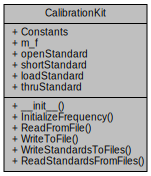
\includegraphics[width=223pt]{classSignalIntegrity_1_1Measurement_1_1CalKit_1_1CalibrationKit_1_1CalibrationKit__coll__graph}
\end{center}
\end{figure}
\subsection*{Public Member Functions}
\begin{DoxyCompactItemize}
\item 
def \hyperlink{classSignalIntegrity_1_1Measurement_1_1CalKit_1_1CalibrationKit_1_1CalibrationKit_a7c969c556643c62769436aaee9bee342}{\+\_\+\+\_\+init\+\_\+\+\_\+} (self, filename=None, f=None)
\begin{DoxyCompactList}\small\item\em Constructor. \end{DoxyCompactList}\item 
def \hyperlink{classSignalIntegrity_1_1Measurement_1_1CalKit_1_1CalibrationKit_1_1CalibrationKit_a068ffbf43377a9e28cccb8b6013772ea}{Initialize\+Frequency} (self, f)
\begin{DoxyCompactList}\small\item\em Initializes frequencies. \end{DoxyCompactList}\item 
def \hyperlink{classSignalIntegrity_1_1Measurement_1_1CalKit_1_1CalibrationKit_1_1CalibrationKit_a3dc78f8134b7196685f6b0b5ace5e33b}{Read\+From\+File} (self, filename)
\begin{DoxyCompactList}\small\item\em Reads the calibration constants from a file. \end{DoxyCompactList}\item 
def \hyperlink{classSignalIntegrity_1_1Measurement_1_1CalKit_1_1CalibrationKit_1_1CalibrationKit_ac68713cc133371d7a733dd318b5669d3}{Write\+To\+File} (self, filename, calkitname=None)
\begin{DoxyCompactList}\small\item\em Write calibration constants to a file. \end{DoxyCompactList}\item 
def \hyperlink{classSignalIntegrity_1_1Measurement_1_1CalKit_1_1CalibrationKit_1_1CalibrationKit_ab30dce63eb90ca31d9bea9036710996a}{Write\+Standards\+To\+Files} (self, filename\+Prefix)
\begin{DoxyCompactList}\small\item\em Writes the standards to s-\/parameter files. \end{DoxyCompactList}\item 
def \hyperlink{classSignalIntegrity_1_1Measurement_1_1CalKit_1_1CalibrationKit_1_1CalibrationKit_a749305349102d6e6bfd1babeb152046f}{Read\+Standards\+From\+Files} (self, filename\+Prefix)
\begin{DoxyCompactList}\small\item\em Reads the standards from s-\/parameter files. \end{DoxyCompactList}\end{DoxyCompactItemize}
\subsection*{Public Attributes}
\begin{DoxyCompactItemize}
\item 
\mbox{\Hypertarget{classSignalIntegrity_1_1Measurement_1_1CalKit_1_1CalibrationKit_1_1CalibrationKit_a198b8c2c77ea9f9815a181ddeda1c320}\label{classSignalIntegrity_1_1Measurement_1_1CalKit_1_1CalibrationKit_1_1CalibrationKit_a198b8c2c77ea9f9815a181ddeda1c320}} 
\hyperlink{classSignalIntegrity_1_1Measurement_1_1CalKit_1_1CalibrationKit_1_1CalibrationKit_a198b8c2c77ea9f9815a181ddeda1c320}{Constants}
\begin{DoxyCompactList}\small\item\em instance of class \hyperlink{classSignalIntegrity_1_1Measurement_1_1CalKit_1_1CalibrationKit_1_1CalibrationConstants}{Calibration\+Constants} containing the calibration constants. \end{DoxyCompactList}\item 
\mbox{\Hypertarget{classSignalIntegrity_1_1Measurement_1_1CalKit_1_1CalibrationKit_1_1CalibrationKit_a40a26fb5046a51e40dd1b61c78d72ace}\label{classSignalIntegrity_1_1Measurement_1_1CalKit_1_1CalibrationKit_1_1CalibrationKit_a40a26fb5046a51e40dd1b61c78d72ace}} 
\hyperlink{classSignalIntegrity_1_1Measurement_1_1CalKit_1_1CalibrationKit_1_1CalibrationKit_a40a26fb5046a51e40dd1b61c78d72ace}{m\+\_\+f}
\begin{DoxyCompactList}\small\item\em list of frequencies \end{DoxyCompactList}\item 
\hyperlink{classSignalIntegrity_1_1Measurement_1_1CalKit_1_1CalibrationKit_1_1CalibrationKit_adfa88578140d393e4fc3d5e6976c4586}{open\+Standard}
\begin{DoxyCompactList}\small\item\em instance of class \hyperlink{namespaceSignalIntegrity_1_1SParameters}{S\+Parameters} containing s-\/parameters of an open standard corresponding to frequencies provided and calibration constants. \end{DoxyCompactList}\item 
\hyperlink{classSignalIntegrity_1_1Measurement_1_1CalKit_1_1CalibrationKit_1_1CalibrationKit_a094c01f8f3b9b22b8759481b3d5bdb85}{short\+Standard}
\begin{DoxyCompactList}\small\item\em instance of class \hyperlink{namespaceSignalIntegrity_1_1SParameters}{S\+Parameters} containing s-\/parameters of a short standard corresponding to frequencies provided and calibration constants. \end{DoxyCompactList}\item 
\hyperlink{classSignalIntegrity_1_1Measurement_1_1CalKit_1_1CalibrationKit_1_1CalibrationKit_af4b585ef48fed700d70b2bee7e5ffdbe}{load\+Standard}
\begin{DoxyCompactList}\small\item\em instance of class \hyperlink{namespaceSignalIntegrity_1_1SParameters}{S\+Parameters} containing s-\/parameters of a load standard corresponding to frequencies provided and calibration constants. \end{DoxyCompactList}\item 
\hyperlink{classSignalIntegrity_1_1Measurement_1_1CalKit_1_1CalibrationKit_1_1CalibrationKit_a63691e31dc0a91dbcfe40635f9c87599}{thru\+Standard}
\begin{DoxyCompactList}\small\item\em instance of class \hyperlink{namespaceSignalIntegrity_1_1SParameters}{S\+Parameters} containing s-\/parameters of a thru standard corresponding to frequencies provided and calibration constants. \end{DoxyCompactList}\end{DoxyCompactItemize}


\subsection{Detailed Description}
Class for holding a calibration kit derived from calibration constants. 

Definition at line 303 of file Calibration\+Kit.\+py.



\subsection{Constructor \& Destructor Documentation}
\mbox{\Hypertarget{classSignalIntegrity_1_1Measurement_1_1CalKit_1_1CalibrationKit_1_1CalibrationKit_a7c969c556643c62769436aaee9bee342}\label{classSignalIntegrity_1_1Measurement_1_1CalKit_1_1CalibrationKit_1_1CalibrationKit_a7c969c556643c62769436aaee9bee342}} 
\index{Signal\+Integrity\+::\+Measurement\+::\+Cal\+Kit\+::\+Calibration\+Kit\+::\+Calibration\+Kit@{Signal\+Integrity\+::\+Measurement\+::\+Cal\+Kit\+::\+Calibration\+Kit\+::\+Calibration\+Kit}!\+\_\+\+\_\+init\+\_\+\+\_\+@{\+\_\+\+\_\+init\+\_\+\+\_\+}}
\index{\+\_\+\+\_\+init\+\_\+\+\_\+@{\+\_\+\+\_\+init\+\_\+\+\_\+}!Signal\+Integrity\+::\+Measurement\+::\+Cal\+Kit\+::\+Calibration\+Kit\+::\+Calibration\+Kit@{Signal\+Integrity\+::\+Measurement\+::\+Cal\+Kit\+::\+Calibration\+Kit\+::\+Calibration\+Kit}}
\subsubsection{\texorpdfstring{\+\_\+\+\_\+init\+\_\+\+\_\+()}{\_\_init\_\_()}}
{\footnotesize\ttfamily def \+\_\+\+\_\+init\+\_\+\+\_\+ (\begin{DoxyParamCaption}\item[{}]{self,  }\item[{}]{filename = {\ttfamily None},  }\item[{}]{f = {\ttfamily None} }\end{DoxyParamCaption})}



Constructor. 


\begin{DoxyParams}{Parameters}
{\em filename} & (optional) string filename of calibration constants file to read. \\
\hline
{\em f} & (optional) list of frequencies to define the calibration standards for. The calibration constants are initialized to their default as specified in \hyperlink{classSignalIntegrity_1_1Measurement_1_1CalKit_1_1CalibrationKit_1_1CalibrationConstants_ae64f0875afe3067b97ba370b354b9213}{Calibration\+Constants.\+\_\+\+\_\+init\+\_\+\+\_\+()}.\\
\hline
\end{DoxyParams}
If a filename is specified, the calibration constants are read from the disk.

If frequencies are provided, the frequencies are initialized and the calibration standards are initialized to have the s-\/parameters of the standards as defined by the frequencies and calibration constants.

No calibration standards are generated yet if no frequencies are provided. \begin{DoxySeeAlso}{See also}
Intialize\+Frequency 
\end{DoxySeeAlso}


Definition at line 318 of file Calibration\+Kit.\+py.



\subsection{Member Function Documentation}
\mbox{\Hypertarget{classSignalIntegrity_1_1Measurement_1_1CalKit_1_1CalibrationKit_1_1CalibrationKit_a068ffbf43377a9e28cccb8b6013772ea}\label{classSignalIntegrity_1_1Measurement_1_1CalKit_1_1CalibrationKit_1_1CalibrationKit_a068ffbf43377a9e28cccb8b6013772ea}} 
\index{Signal\+Integrity\+::\+Measurement\+::\+Cal\+Kit\+::\+Calibration\+Kit\+::\+Calibration\+Kit@{Signal\+Integrity\+::\+Measurement\+::\+Cal\+Kit\+::\+Calibration\+Kit\+::\+Calibration\+Kit}!Initialize\+Frequency@{Initialize\+Frequency}}
\index{Initialize\+Frequency@{Initialize\+Frequency}!Signal\+Integrity\+::\+Measurement\+::\+Cal\+Kit\+::\+Calibration\+Kit\+::\+Calibration\+Kit@{Signal\+Integrity\+::\+Measurement\+::\+Cal\+Kit\+::\+Calibration\+Kit\+::\+Calibration\+Kit}}
\subsubsection{\texorpdfstring{Initialize\+Frequency()}{InitializeFrequency()}}
{\footnotesize\ttfamily def Initialize\+Frequency (\begin{DoxyParamCaption}\item[{}]{self,  }\item[{}]{f }\end{DoxyParamCaption})}



Initializes frequencies. 


\begin{DoxyParams}{Parameters}
{\em f} & list of frequencies \hyperlink{namespaceSignalIntegrity_1_1Measurement_1_1Calibration}{Calibration} standards are initialized to have the s-\/parameters of the standards as defined by the frequencies and calibration constants.\\
\hline
\end{DoxyParams}
Once intialized, the s-\/parameters of the calibration standards can be accessed and used. \begin{DoxySeeAlso}{See also}
\hyperlink{classSignalIntegrity_1_1Measurement_1_1CalKit_1_1CalibrationKit_1_1CalibrationKit_adfa88578140d393e4fc3d5e6976c4586}{open\+Standard} 

\hyperlink{classSignalIntegrity_1_1Measurement_1_1CalKit_1_1CalibrationKit_1_1CalibrationKit_a094c01f8f3b9b22b8759481b3d5bdb85}{short\+Standard} 

\hyperlink{classSignalIntegrity_1_1Measurement_1_1CalKit_1_1CalibrationKit_1_1CalibrationKit_af4b585ef48fed700d70b2bee7e5ffdbe}{load\+Standard} 

\hyperlink{classSignalIntegrity_1_1Measurement_1_1CalKit_1_1CalibrationKit_1_1CalibrationKit_a63691e31dc0a91dbcfe40635f9c87599}{thru\+Standard} 
\end{DoxySeeAlso}


Definition at line 337 of file Calibration\+Kit.\+py.

\mbox{\Hypertarget{classSignalIntegrity_1_1Measurement_1_1CalKit_1_1CalibrationKit_1_1CalibrationKit_a3dc78f8134b7196685f6b0b5ace5e33b}\label{classSignalIntegrity_1_1Measurement_1_1CalKit_1_1CalibrationKit_1_1CalibrationKit_a3dc78f8134b7196685f6b0b5ace5e33b}} 
\index{Signal\+Integrity\+::\+Measurement\+::\+Cal\+Kit\+::\+Calibration\+Kit\+::\+Calibration\+Kit@{Signal\+Integrity\+::\+Measurement\+::\+Cal\+Kit\+::\+Calibration\+Kit\+::\+Calibration\+Kit}!Read\+From\+File@{Read\+From\+File}}
\index{Read\+From\+File@{Read\+From\+File}!Signal\+Integrity\+::\+Measurement\+::\+Cal\+Kit\+::\+Calibration\+Kit\+::\+Calibration\+Kit@{Signal\+Integrity\+::\+Measurement\+::\+Cal\+Kit\+::\+Calibration\+Kit\+::\+Calibration\+Kit}}
\subsubsection{\texorpdfstring{Read\+From\+File()}{ReadFromFile()}}
{\footnotesize\ttfamily def Read\+From\+File (\begin{DoxyParamCaption}\item[{}]{self,  }\item[{}]{filename }\end{DoxyParamCaption})}



Reads the calibration constants from a file. 


\begin{DoxyParams}{Parameters}
{\em filename} & string name of file to read calibration constants from \\
\hline
\end{DoxyParams}
\begin{DoxyReturn}{Returns}
self 
\end{DoxyReturn}
\begin{DoxySeeAlso}{See also}
\hyperlink{classSignalIntegrity_1_1Measurement_1_1CalKit_1_1CalibrationKit_1_1CalibrationConstants_a3dc78f8134b7196685f6b0b5ace5e33b}{Calibration\+Constants.\+Read\+From\+File()} 

\hyperlink{classSignalIntegrity_1_1Measurement_1_1CalKit_1_1CalibrationKit_1_1CalibrationConstants}{Calibration\+Constants} for file format 
\end{DoxySeeAlso}


Definition at line 360 of file Calibration\+Kit.\+py.

\mbox{\Hypertarget{classSignalIntegrity_1_1Measurement_1_1CalKit_1_1CalibrationKit_1_1CalibrationKit_a749305349102d6e6bfd1babeb152046f}\label{classSignalIntegrity_1_1Measurement_1_1CalKit_1_1CalibrationKit_1_1CalibrationKit_a749305349102d6e6bfd1babeb152046f}} 
\index{Signal\+Integrity\+::\+Measurement\+::\+Cal\+Kit\+::\+Calibration\+Kit\+::\+Calibration\+Kit@{Signal\+Integrity\+::\+Measurement\+::\+Cal\+Kit\+::\+Calibration\+Kit\+::\+Calibration\+Kit}!Read\+Standards\+From\+Files@{Read\+Standards\+From\+Files}}
\index{Read\+Standards\+From\+Files@{Read\+Standards\+From\+Files}!Signal\+Integrity\+::\+Measurement\+::\+Cal\+Kit\+::\+Calibration\+Kit\+::\+Calibration\+Kit@{Signal\+Integrity\+::\+Measurement\+::\+Cal\+Kit\+::\+Calibration\+Kit\+::\+Calibration\+Kit}}
\subsubsection{\texorpdfstring{Read\+Standards\+From\+Files()}{ReadStandardsFromFiles()}}
{\footnotesize\ttfamily def Read\+Standards\+From\+Files (\begin{DoxyParamCaption}\item[{}]{self,  }\item[{}]{filename\+Prefix }\end{DoxyParamCaption})}



Reads the standards from s-\/parameter files. 


\begin{DoxyParams}{Parameters}
{\em filename\+Prefix} & string name of prefix for standards file names \\
\hline
\end{DoxyParams}
\begin{DoxyReturn}{Returns}
self Each standard is prefixed with the filename\+Prefix provided concatenated with\+:
\begin{DoxyItemize}
\item \textquotesingle{}Short.\+s1p\textquotesingle{} -\/ for the short standard.
\item \textquotesingle{}Open.\+s1p\textquotesingle{} -\/ for the open standard.
\item \textquotesingle{}Load.\+s1p\textquotesingle{} -\/ for the load standard.
\item \textquotesingle{}Thru.\+s2p\textquotesingle{} -\/ for the thru standard 
\end{DoxyItemize}
\end{DoxyReturn}
\begin{DoxyAttention}{Attention}
This decouples the standards from the calibration constants and is not preferred. 
\end{DoxyAttention}
\begin{DoxySeeAlso}{See also}
\hyperlink{classSignalIntegrity_1_1Measurement_1_1CalKit_1_1CalibrationKit_1_1CalibrationKit_a094c01f8f3b9b22b8759481b3d5bdb85}{short\+Standard} 

\hyperlink{classSignalIntegrity_1_1Measurement_1_1CalKit_1_1CalibrationKit_1_1CalibrationKit_adfa88578140d393e4fc3d5e6976c4586}{open\+Standard} 

\hyperlink{classSignalIntegrity_1_1Measurement_1_1CalKit_1_1CalibrationKit_1_1CalibrationKit_af4b585ef48fed700d70b2bee7e5ffdbe}{load\+Standard} 

\hyperlink{classSignalIntegrity_1_1Measurement_1_1CalKit_1_1CalibrationKit_1_1CalibrationKit_a63691e31dc0a91dbcfe40635f9c87599}{thru\+Standard} 
\end{DoxySeeAlso}


Definition at line 410 of file Calibration\+Kit.\+py.

\mbox{\Hypertarget{classSignalIntegrity_1_1Measurement_1_1CalKit_1_1CalibrationKit_1_1CalibrationKit_ab30dce63eb90ca31d9bea9036710996a}\label{classSignalIntegrity_1_1Measurement_1_1CalKit_1_1CalibrationKit_1_1CalibrationKit_ab30dce63eb90ca31d9bea9036710996a}} 
\index{Signal\+Integrity\+::\+Measurement\+::\+Cal\+Kit\+::\+Calibration\+Kit\+::\+Calibration\+Kit@{Signal\+Integrity\+::\+Measurement\+::\+Cal\+Kit\+::\+Calibration\+Kit\+::\+Calibration\+Kit}!Write\+Standards\+To\+Files@{Write\+Standards\+To\+Files}}
\index{Write\+Standards\+To\+Files@{Write\+Standards\+To\+Files}!Signal\+Integrity\+::\+Measurement\+::\+Cal\+Kit\+::\+Calibration\+Kit\+::\+Calibration\+Kit@{Signal\+Integrity\+::\+Measurement\+::\+Cal\+Kit\+::\+Calibration\+Kit\+::\+Calibration\+Kit}}
\subsubsection{\texorpdfstring{Write\+Standards\+To\+Files()}{WriteStandardsToFiles()}}
{\footnotesize\ttfamily def Write\+Standards\+To\+Files (\begin{DoxyParamCaption}\item[{}]{self,  }\item[{}]{filename\+Prefix }\end{DoxyParamCaption})}



Writes the standards to s-\/parameter files. 


\begin{DoxyParams}{Parameters}
{\em filename\+Prefix} & string name of prefix for standards file names \\
\hline
\end{DoxyParams}
\begin{DoxyReturn}{Returns}
self Each standard is prefixed with the filename\+Prefix provided concatenated with\+:
\begin{DoxyItemize}
\item \textquotesingle{}Short.\+s1p\textquotesingle{} -\/ for the short standard.
\item \textquotesingle{}Open.\+s1p\textquotesingle{} -\/ for the open standard.
\item \textquotesingle{}Load.\+s1p\textquotesingle{} -\/ for the load standard.
\item \textquotesingle{}Thru.\+s2p\textquotesingle{} -\/ for the thru standard 
\end{DoxyItemize}
\end{DoxyReturn}
\begin{DoxyAttention}{Attention}
the member variables for the standards must exist. 
\end{DoxyAttention}
\begin{DoxySeeAlso}{See also}
\hyperlink{classSignalIntegrity_1_1Measurement_1_1CalKit_1_1CalibrationKit_1_1CalibrationKit_a094c01f8f3b9b22b8759481b3d5bdb85}{short\+Standard} 

\hyperlink{classSignalIntegrity_1_1Measurement_1_1CalKit_1_1CalibrationKit_1_1CalibrationKit_adfa88578140d393e4fc3d5e6976c4586}{open\+Standard} 

\hyperlink{classSignalIntegrity_1_1Measurement_1_1CalKit_1_1CalibrationKit_1_1CalibrationKit_af4b585ef48fed700d70b2bee7e5ffdbe}{load\+Standard} 

\hyperlink{classSignalIntegrity_1_1Measurement_1_1CalKit_1_1CalibrationKit_1_1CalibrationKit_a63691e31dc0a91dbcfe40635f9c87599}{thru\+Standard} 
\end{DoxySeeAlso}


Definition at line 389 of file Calibration\+Kit.\+py.

\mbox{\Hypertarget{classSignalIntegrity_1_1Measurement_1_1CalKit_1_1CalibrationKit_1_1CalibrationKit_ac68713cc133371d7a733dd318b5669d3}\label{classSignalIntegrity_1_1Measurement_1_1CalKit_1_1CalibrationKit_1_1CalibrationKit_ac68713cc133371d7a733dd318b5669d3}} 
\index{Signal\+Integrity\+::\+Measurement\+::\+Cal\+Kit\+::\+Calibration\+Kit\+::\+Calibration\+Kit@{Signal\+Integrity\+::\+Measurement\+::\+Cal\+Kit\+::\+Calibration\+Kit\+::\+Calibration\+Kit}!Write\+To\+File@{Write\+To\+File}}
\index{Write\+To\+File@{Write\+To\+File}!Signal\+Integrity\+::\+Measurement\+::\+Cal\+Kit\+::\+Calibration\+Kit\+::\+Calibration\+Kit@{Signal\+Integrity\+::\+Measurement\+::\+Cal\+Kit\+::\+Calibration\+Kit\+::\+Calibration\+Kit}}
\subsubsection{\texorpdfstring{Write\+To\+File()}{WriteToFile()}}
{\footnotesize\ttfamily def Write\+To\+File (\begin{DoxyParamCaption}\item[{}]{self,  }\item[{}]{filename,  }\item[{}]{calkitname = {\ttfamily None} }\end{DoxyParamCaption})}



Write calibration constants to a file. 


\begin{DoxyParams}{Parameters}
{\em filename} & string name of calibration constant file to write \\
\hline
{\em calkitname} & (optional) string containing header information to be placed after the D\+E\+S\+C\+R\+I\+P\+T\+I\+ON\+: in the header information. \\
\hline
\end{DoxyParams}
\begin{DoxyReturn}{Returns}
self 
\end{DoxyReturn}
\begin{DoxySeeAlso}{See also}
\hyperlink{classSignalIntegrity_1_1Measurement_1_1CalKit_1_1CalibrationKit_1_1CalibrationConstants_ac68713cc133371d7a733dd318b5669d3}{Calibration\+Constants.\+Write\+To\+File()} 
\end{DoxySeeAlso}


Definition at line 371 of file Calibration\+Kit.\+py.



\subsection{Member Data Documentation}
\mbox{\Hypertarget{classSignalIntegrity_1_1Measurement_1_1CalKit_1_1CalibrationKit_1_1CalibrationKit_af4b585ef48fed700d70b2bee7e5ffdbe}\label{classSignalIntegrity_1_1Measurement_1_1CalKit_1_1CalibrationKit_1_1CalibrationKit_af4b585ef48fed700d70b2bee7e5ffdbe}} 
\index{Signal\+Integrity\+::\+Measurement\+::\+Cal\+Kit\+::\+Calibration\+Kit\+::\+Calibration\+Kit@{Signal\+Integrity\+::\+Measurement\+::\+Cal\+Kit\+::\+Calibration\+Kit\+::\+Calibration\+Kit}!load\+Standard@{load\+Standard}}
\index{load\+Standard@{load\+Standard}!Signal\+Integrity\+::\+Measurement\+::\+Cal\+Kit\+::\+Calibration\+Kit\+::\+Calibration\+Kit@{Signal\+Integrity\+::\+Measurement\+::\+Cal\+Kit\+::\+Calibration\+Kit\+::\+Calibration\+Kit}}
\subsubsection{\texorpdfstring{load\+Standard}{loadStandard}}
{\footnotesize\ttfamily load\+Standard}



instance of class \hyperlink{namespaceSignalIntegrity_1_1SParameters}{S\+Parameters} containing s-\/parameters of a load standard corresponding to frequencies provided and calibration constants. 

\begin{DoxyAttention}{Attention}
this only defined if the class was initialized with a frequency list or a call was made to \hyperlink{classSignalIntegrity_1_1Measurement_1_1CalKit_1_1CalibrationKit_1_1CalibrationKit_a068ffbf43377a9e28cccb8b6013772ea}{Initialize\+Frequency()} 
\end{DoxyAttention}


Definition at line 347 of file Calibration\+Kit.\+py.

\mbox{\Hypertarget{classSignalIntegrity_1_1Measurement_1_1CalKit_1_1CalibrationKit_1_1CalibrationKit_adfa88578140d393e4fc3d5e6976c4586}\label{classSignalIntegrity_1_1Measurement_1_1CalKit_1_1CalibrationKit_1_1CalibrationKit_adfa88578140d393e4fc3d5e6976c4586}} 
\index{Signal\+Integrity\+::\+Measurement\+::\+Cal\+Kit\+::\+Calibration\+Kit\+::\+Calibration\+Kit@{Signal\+Integrity\+::\+Measurement\+::\+Cal\+Kit\+::\+Calibration\+Kit\+::\+Calibration\+Kit}!open\+Standard@{open\+Standard}}
\index{open\+Standard@{open\+Standard}!Signal\+Integrity\+::\+Measurement\+::\+Cal\+Kit\+::\+Calibration\+Kit\+::\+Calibration\+Kit@{Signal\+Integrity\+::\+Measurement\+::\+Cal\+Kit\+::\+Calibration\+Kit\+::\+Calibration\+Kit}}
\subsubsection{\texorpdfstring{open\+Standard}{openStandard}}
{\footnotesize\ttfamily open\+Standard}



instance of class \hyperlink{namespaceSignalIntegrity_1_1SParameters}{S\+Parameters} containing s-\/parameters of an open standard corresponding to frequencies provided and calibration constants. 

\begin{DoxyAttention}{Attention}
this only defined if the class was initialized with a frequency list or a call was made to \hyperlink{classSignalIntegrity_1_1Measurement_1_1CalKit_1_1CalibrationKit_1_1CalibrationKit_a068ffbf43377a9e28cccb8b6013772ea}{Initialize\+Frequency()} 
\end{DoxyAttention}


Definition at line 339 of file Calibration\+Kit.\+py.

\mbox{\Hypertarget{classSignalIntegrity_1_1Measurement_1_1CalKit_1_1CalibrationKit_1_1CalibrationKit_a094c01f8f3b9b22b8759481b3d5bdb85}\label{classSignalIntegrity_1_1Measurement_1_1CalKit_1_1CalibrationKit_1_1CalibrationKit_a094c01f8f3b9b22b8759481b3d5bdb85}} 
\index{Signal\+Integrity\+::\+Measurement\+::\+Cal\+Kit\+::\+Calibration\+Kit\+::\+Calibration\+Kit@{Signal\+Integrity\+::\+Measurement\+::\+Cal\+Kit\+::\+Calibration\+Kit\+::\+Calibration\+Kit}!short\+Standard@{short\+Standard}}
\index{short\+Standard@{short\+Standard}!Signal\+Integrity\+::\+Measurement\+::\+Cal\+Kit\+::\+Calibration\+Kit\+::\+Calibration\+Kit@{Signal\+Integrity\+::\+Measurement\+::\+Cal\+Kit\+::\+Calibration\+Kit\+::\+Calibration\+Kit}}
\subsubsection{\texorpdfstring{short\+Standard}{shortStandard}}
{\footnotesize\ttfamily short\+Standard}



instance of class \hyperlink{namespaceSignalIntegrity_1_1SParameters}{S\+Parameters} containing s-\/parameters of a short standard corresponding to frequencies provided and calibration constants. 

\begin{DoxyAttention}{Attention}
this only defined if the class was initialized with a frequency list or a call was made to \hyperlink{classSignalIntegrity_1_1Measurement_1_1CalKit_1_1CalibrationKit_1_1CalibrationKit_a068ffbf43377a9e28cccb8b6013772ea}{Initialize\+Frequency()} 
\end{DoxyAttention}


Definition at line 343 of file Calibration\+Kit.\+py.

\mbox{\Hypertarget{classSignalIntegrity_1_1Measurement_1_1CalKit_1_1CalibrationKit_1_1CalibrationKit_a63691e31dc0a91dbcfe40635f9c87599}\label{classSignalIntegrity_1_1Measurement_1_1CalKit_1_1CalibrationKit_1_1CalibrationKit_a63691e31dc0a91dbcfe40635f9c87599}} 
\index{Signal\+Integrity\+::\+Measurement\+::\+Cal\+Kit\+::\+Calibration\+Kit\+::\+Calibration\+Kit@{Signal\+Integrity\+::\+Measurement\+::\+Cal\+Kit\+::\+Calibration\+Kit\+::\+Calibration\+Kit}!thru\+Standard@{thru\+Standard}}
\index{thru\+Standard@{thru\+Standard}!Signal\+Integrity\+::\+Measurement\+::\+Cal\+Kit\+::\+Calibration\+Kit\+::\+Calibration\+Kit@{Signal\+Integrity\+::\+Measurement\+::\+Cal\+Kit\+::\+Calibration\+Kit\+::\+Calibration\+Kit}}
\subsubsection{\texorpdfstring{thru\+Standard}{thruStandard}}
{\footnotesize\ttfamily thru\+Standard}



instance of class \hyperlink{namespaceSignalIntegrity_1_1SParameters}{S\+Parameters} containing s-\/parameters of a thru standard corresponding to frequencies provided and calibration constants. 

\begin{DoxyAttention}{Attention}
this only defined if the class was initialized with a frequency list or a call was made to \hyperlink{classSignalIntegrity_1_1Measurement_1_1CalKit_1_1CalibrationKit_1_1CalibrationKit_a068ffbf43377a9e28cccb8b6013772ea}{Initialize\+Frequency()} 
\end{DoxyAttention}


Definition at line 350 of file Calibration\+Kit.\+py.



The documentation for this class was generated from the following file\+:\begin{DoxyCompactItemize}
\item 
Py\+S\+I/\+Signal\+Integrity/\+Measurement/\+Cal\+Kit/Calibration\+Kit.\+py\end{DoxyCompactItemize}

\hypertarget{classSignalIntegrity_1_1Measurement_1_1Calibration_1_1CalibrationMeasurements_1_1CalibrationMeasurement}{}\section{Calibration\+Measurement Class Reference}
\label{classSignalIntegrity_1_1Measurement_1_1Calibration_1_1CalibrationMeasurements_1_1CalibrationMeasurement}\index{Calibration\+Measurement@{Calibration\+Measurement}}


\hyperlink{namespaceSignalIntegrity_1_1Measurement_1_1Calibration_1_1Calibration}{Calibration} Measurements.  




Inheritance diagram for Calibration\+Measurement\+:
\nopagebreak
\begin{figure}[H]
\begin{center}
\leavevmode
\includegraphics[width=350pt]{classSignalIntegrity_1_1Measurement_1_1Calibration_1_1CalibrationMeasurements_1_1CalibrationMeasurement__inherit__graph}
\end{center}
\end{figure}


Collaboration diagram for Calibration\+Measurement\+:
\nopagebreak
\begin{figure}[H]
\begin{center}
\leavevmode
\includegraphics[width=202pt]{classSignalIntegrity_1_1Measurement_1_1Calibration_1_1CalibrationMeasurements_1_1CalibrationMeasurement__coll__graph}
\end{center}
\end{figure}
\subsection*{Public Member Functions}
\begin{DoxyCompactItemize}
\item 
def \hyperlink{classSignalIntegrity_1_1Measurement_1_1Calibration_1_1CalibrationMeasurements_1_1CalibrationMeasurement_a1ddf400813e458d6de6ee54246f050e7}{\+\_\+\+\_\+init\+\_\+\+\_\+} (self, type, name=None)
\begin{DoxyCompactList}\small\item\em Constructor. \end{DoxyCompactList}\end{DoxyCompactItemize}


\subsection{Detailed Description}
\hyperlink{namespaceSignalIntegrity_1_1Measurement_1_1Calibration_1_1Calibration}{Calibration} Measurements. 

Copyright (c) 2018 Teledyne Le\+Croy, all rights reserved worldwide.

This file is part of Py\+SI.

Py\+SI is free software\+: You can redistribute it and/or modify it under the terms of the G\+NU General Public License as published by the Free Software Foundation, either version 3 of the License, or any later version.

This program is distrbuted in the hope that it will be useful, but W\+I\+T\+H\+O\+UT A\+NY W\+A\+R\+R\+A\+N\+TY; without even the implied warranty of M\+E\+R\+C\+H\+A\+N\+T\+A\+B\+I\+L\+I\+TY or F\+I\+T\+N\+E\+SS F\+OR A P\+A\+R\+T\+I\+C\+U\+L\+AR P\+U\+R\+P\+O\+SE. See the G\+NU General Public License for more details.

You should have received a copy of the G\+NU General Public License along with this program. If not, see \href{https://www.gnu.org/licenses/}{\tt https\+://www.\+gnu.\+org/licenses/} Base class for calibration measurements 

Definition at line 23 of file Calibration\+Measurements.\+py.



\subsection{Constructor \& Destructor Documentation}
\mbox{\Hypertarget{classSignalIntegrity_1_1Measurement_1_1Calibration_1_1CalibrationMeasurements_1_1CalibrationMeasurement_a1ddf400813e458d6de6ee54246f050e7}\label{classSignalIntegrity_1_1Measurement_1_1Calibration_1_1CalibrationMeasurements_1_1CalibrationMeasurement_a1ddf400813e458d6de6ee54246f050e7}} 
\index{Signal\+Integrity\+::\+Measurement\+::\+Calibration\+::\+Calibration\+Measurements\+::\+Calibration\+Measurement@{Signal\+Integrity\+::\+Measurement\+::\+Calibration\+::\+Calibration\+Measurements\+::\+Calibration\+Measurement}!\+\_\+\+\_\+init\+\_\+\+\_\+@{\+\_\+\+\_\+init\+\_\+\+\_\+}}
\index{\+\_\+\+\_\+init\+\_\+\+\_\+@{\+\_\+\+\_\+init\+\_\+\+\_\+}!Signal\+Integrity\+::\+Measurement\+::\+Calibration\+::\+Calibration\+Measurements\+::\+Calibration\+Measurement@{Signal\+Integrity\+::\+Measurement\+::\+Calibration\+::\+Calibration\+Measurements\+::\+Calibration\+Measurement}}
\subsubsection{\texorpdfstring{\+\_\+\+\_\+init\+\_\+\+\_\+()}{\_\_init\_\_()}}
{\footnotesize\ttfamily def \+\_\+\+\_\+init\+\_\+\+\_\+ (\begin{DoxyParamCaption}\item[{}]{self,  }\item[{}]{type,  }\item[{}]{name = {\ttfamily None} }\end{DoxyParamCaption})}



Constructor. 


\begin{DoxyParams}{Parameters}
{\em type} & string representing the type of the measurement. \\
\hline
{\em name} & (optional) string representing the name of the measurement \\
\hline
\end{DoxyParams}
\begin{DoxyRemark}{Remarks}
The name of the measurement is not used for anything, but can be used to identify the name of a calibration measurement externally.
\end{DoxyRemark}
valid types of calibration measurements are\+:


\begin{DoxyItemize}
\item \textquotesingle{}reflect\textquotesingle{} -\/ a reflect measurement taken on a port with a reflect standard (like short, open, or load).
\item \textquotesingle{}thru\textquotesingle{} -\/ a thru calibration measurement taken between two ports.
\item \textquotesingle{}xtalk\textquotesingle{} -\/ a crosstalk calibration measurement typically taken between two ports that are completely unconnected. \begin{DoxySeeAlso}{See also}
\hyperlink{classSignalIntegrity_1_1Measurement_1_1Calibration_1_1CalibrationMeasurements_1_1ReflectCalibrationMeasurement}{Reflect\+Calibration\+Measurement} 

\hyperlink{classSignalIntegrity_1_1Measurement_1_1Calibration_1_1CalibrationMeasurements_1_1ThruCalibrationMeasurement}{Thru\+Calibration\+Measurement} 

\hyperlink{classSignalIntegrity_1_1Measurement_1_1Calibration_1_1CalibrationMeasurements_1_1XtalkCalibrationMeasurement}{Xtalk\+Calibration\+Measurement} 
\end{DoxySeeAlso}

\end{DoxyItemize}

Definition at line 43 of file Calibration\+Measurements.\+py.



The documentation for this class was generated from the following file\+:\begin{DoxyCompactItemize}
\item 
Py\+S\+I/\+Signal\+Integrity/\+Measurement/\+Calibration/Calibration\+Measurements.\+py\end{DoxyCompactItemize}

\hypertarget{classSignalIntegrity_1_1CallBacker_1_1CallBacker}{}\section{Call\+Backer Class Reference}
\label{classSignalIntegrity_1_1CallBacker_1_1CallBacker}\index{Call\+Backer@{Call\+Backer}}


Handles Callbacks that allow progress reporting during long calculations and capability to abort.  




Inheritance diagram for Call\+Backer\+:\nopagebreak
\begin{figure}[H]
\begin{center}
\leavevmode
\includegraphics[width=350pt]{classSignalIntegrity_1_1CallBacker_1_1CallBacker__inherit__graph}
\end{center}
\end{figure}


Collaboration diagram for Call\+Backer\+:\nopagebreak
\begin{figure}[H]
\begin{center}
\leavevmode
\includegraphics[width=187pt]{classSignalIntegrity_1_1CallBacker_1_1CallBacker__coll__graph}
\end{center}
\end{figure}
\subsection*{Public Member Functions}
\begin{DoxyCompactItemize}
\item 
def \hyperlink{classSignalIntegrity_1_1CallBacker_1_1CallBacker_a5580a7fcf0bfd317a8f8c7c80eefdd69}{\+\_\+\+\_\+init\+\_\+\+\_\+} (self, callback=None)
\begin{DoxyCompactList}\small\item\em Constructor. \end{DoxyCompactList}\item 
def \hyperlink{classSignalIntegrity_1_1CallBacker_1_1CallBacker_ad1aebee41f7b067b9fc11c28f87b27ba}{Call\+Back} (self, progress\+Percent)
\begin{DoxyCompactList}\small\item\em This function is called periodically, which in turn calls any installed callback function. \end{DoxyCompactList}\item 
def \hyperlink{classSignalIntegrity_1_1CallBacker_1_1CallBacker_a9307eb7d2258b5f1df8bfc5f43effcab}{Install\+Callback} (self, callback=None)
\begin{DoxyCompactList}\small\item\em This is an alternate way to supply the callback, if it cannot be installed during initialization of the derived class. \end{DoxyCompactList}\item 
def \hyperlink{classSignalIntegrity_1_1CallBacker_1_1CallBacker_ac93a2d2ea7a87653318147244b98b31c}{Remove\+Callback} (self)
\begin{DoxyCompactList}\small\item\em Removes any callback previously installed. \end{DoxyCompactList}\end{DoxyCompactItemize}


\subsection{Detailed Description}
Handles Callbacks that allow progress reporting during long calculations and capability to abort. 

Teledyne Le\+Croy Inc. (\char`\"{}\+C\+O\+M\+P\+A\+N\+Y\char`\"{}) C\+O\+N\+F\+I\+D\+E\+N\+T\+I\+AL Unpublished Copyright (c) 2015-\/2016 Peter J. Pupalaikis and Teledyne Le\+Croy, All Rights Reserved.

Explicit license in accompanying R\+E\+A\+D\+M\+E.\+txt file. If you don\textquotesingle{}t have that file or do not agree to the terms in that file, then you are not licensed to use this material whatsoever. \hyperlink{classSignalIntegrity_1_1CallBacker_1_1CallBacker}{Call\+Backer} \begin{DoxyVerb}To use callbacks, a class is derived from CallBacker.

Either the constructor of the derived class or some other mechanism should
provide means for supplying the callback function, which is installed in a
call to __init__.

The derived class, during some long operation, then calls the callback function
periodically.  The callback function then has the opportunity to report its
progress.  Returning False in the callback function should cause the operation
to abort.

Here's a mini example derived class using CallBacker:
\end{DoxyVerb}



\begin{DoxyCode}
\textcolor{keyword}{class }ProcessingClass(Callbacker):
    \textcolor{keyword}{def }\_\_init\_\_(self,callback=None):
        ...
        Callbacker.\_\_init\_\_(callback)
        ...
    \textcolor{keyword}{def }LongProcessingFunction(self):
        \textcolor{keywordflow}{for} m \textcolor{keywordflow}{in} range(100):
            ...
            do some calculating.
            ...
            \textcolor{keywordflow}{if} \textcolor{keywordflow}{not} self.CallBack(m):
                process was aborted
                \textcolor{keywordflow}{return}
\end{DoxyCode}
 

Definition at line 47 of file Call\+Backer.\+py.



\subsection{Constructor \& Destructor Documentation}
\mbox{\Hypertarget{classSignalIntegrity_1_1CallBacker_1_1CallBacker_a5580a7fcf0bfd317a8f8c7c80eefdd69}\label{classSignalIntegrity_1_1CallBacker_1_1CallBacker_a5580a7fcf0bfd317a8f8c7c80eefdd69}} 
\index{Signal\+Integrity\+::\+Call\+Backer\+::\+Call\+Backer@{Signal\+Integrity\+::\+Call\+Backer\+::\+Call\+Backer}!\+\_\+\+\_\+init\+\_\+\+\_\+@{\+\_\+\+\_\+init\+\_\+\+\_\+}}
\index{\+\_\+\+\_\+init\+\_\+\+\_\+@{\+\_\+\+\_\+init\+\_\+\+\_\+}!Signal\+Integrity\+::\+Call\+Backer\+::\+Call\+Backer@{Signal\+Integrity\+::\+Call\+Backer\+::\+Call\+Backer}}
\subsubsection{\texorpdfstring{\+\_\+\+\_\+init\+\_\+\+\_\+()}{\_\_init\_\_()}}
{\footnotesize\ttfamily def \+\_\+\+\_\+init\+\_\+\+\_\+ (\begin{DoxyParamCaption}\item[{}]{self,  }\item[{}]{callback = {\ttfamily None} }\end{DoxyParamCaption})}



Constructor. 


\begin{DoxyParams}{Parameters}
{\em callback} & (optional, defaults to None) a callback function to call The callback function should take a number as an argument, which represents the progress. \\
\hline
\end{DoxyParams}


Definition at line 53 of file Call\+Backer.\+py.



\subsection{Member Function Documentation}
\mbox{\Hypertarget{classSignalIntegrity_1_1CallBacker_1_1CallBacker_ad1aebee41f7b067b9fc11c28f87b27ba}\label{classSignalIntegrity_1_1CallBacker_1_1CallBacker_ad1aebee41f7b067b9fc11c28f87b27ba}} 
\index{Signal\+Integrity\+::\+Call\+Backer\+::\+Call\+Backer@{Signal\+Integrity\+::\+Call\+Backer\+::\+Call\+Backer}!Call\+Back@{Call\+Back}}
\index{Call\+Back@{Call\+Back}!Signal\+Integrity\+::\+Call\+Backer\+::\+Call\+Backer@{Signal\+Integrity\+::\+Call\+Backer\+::\+Call\+Backer}}
\subsubsection{\texorpdfstring{Call\+Back()}{CallBack()}}
{\footnotesize\ttfamily def Call\+Back (\begin{DoxyParamCaption}\item[{}]{self,  }\item[{}]{progress\+Percent }\end{DoxyParamCaption})}



This function is called periodically, which in turn calls any installed callback function. 


\begin{DoxyParams}{Parameters}
{\em progress\+Percent} & the progress in percent \\
\hline
\end{DoxyParams}


Definition at line 62 of file Call\+Backer.\+py.

\mbox{\Hypertarget{classSignalIntegrity_1_1CallBacker_1_1CallBacker_a9307eb7d2258b5f1df8bfc5f43effcab}\label{classSignalIntegrity_1_1CallBacker_1_1CallBacker_a9307eb7d2258b5f1df8bfc5f43effcab}} 
\index{Signal\+Integrity\+::\+Call\+Backer\+::\+Call\+Backer@{Signal\+Integrity\+::\+Call\+Backer\+::\+Call\+Backer}!Install\+Callback@{Install\+Callback}}
\index{Install\+Callback@{Install\+Callback}!Signal\+Integrity\+::\+Call\+Backer\+::\+Call\+Backer@{Signal\+Integrity\+::\+Call\+Backer\+::\+Call\+Backer}}
\subsubsection{\texorpdfstring{Install\+Callback()}{InstallCallback()}}
{\footnotesize\ttfamily def Install\+Callback (\begin{DoxyParamCaption}\item[{}]{self,  }\item[{}]{callback = {\ttfamily None} }\end{DoxyParamCaption})}



This is an alternate way to supply the callback, if it cannot be installed during initialization of the derived class. 


\begin{DoxyParams}{Parameters}
{\em callback} & (optional, defaults to None) a callback function to call The callback function should take a number as an argument, which represents the progress. \\
\hline
\end{DoxyParams}


Definition at line 74 of file Call\+Backer.\+py.

\mbox{\Hypertarget{classSignalIntegrity_1_1CallBacker_1_1CallBacker_ac93a2d2ea7a87653318147244b98b31c}\label{classSignalIntegrity_1_1CallBacker_1_1CallBacker_ac93a2d2ea7a87653318147244b98b31c}} 
\index{Signal\+Integrity\+::\+Call\+Backer\+::\+Call\+Backer@{Signal\+Integrity\+::\+Call\+Backer\+::\+Call\+Backer}!Remove\+Callback@{Remove\+Callback}}
\index{Remove\+Callback@{Remove\+Callback}!Signal\+Integrity\+::\+Call\+Backer\+::\+Call\+Backer@{Signal\+Integrity\+::\+Call\+Backer\+::\+Call\+Backer}}
\subsubsection{\texorpdfstring{Remove\+Callback()}{RemoveCallback()}}
{\footnotesize\ttfamily def Remove\+Callback (\begin{DoxyParamCaption}\item[{}]{self }\end{DoxyParamCaption})}



Removes any callback previously installed. 



Definition at line 78 of file Call\+Backer.\+py.



The documentation for this class was generated from the following file\+:\begin{DoxyCompactItemize}
\item 
Py\+S\+I/\+Signal\+Integrity/Call\+Backer.\+py\end{DoxyCompactItemize}

\hypertarget{classSignalIntegrity_1_1SystemDescriptions_1_1Deembedder_1_1Deembedder}{}\section{Deembedder Class Reference}
\label{classSignalIntegrity_1_1SystemDescriptions_1_1Deembedder_1_1Deembedder}\index{Deembedder@{Deembedder}}


housekeeping base class for deembedders  




Inheritance diagram for Deembedder\+:
\nopagebreak
\begin{figure}[H]
\begin{center}
\leavevmode
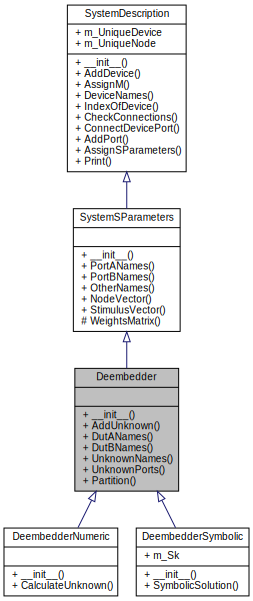
\includegraphics[height=550pt]{classSignalIntegrity_1_1SystemDescriptions_1_1Deembedder_1_1Deembedder__inherit__graph}
\end{center}
\end{figure}


Collaboration diagram for Deembedder\+:
\nopagebreak
\begin{figure}[H]
\begin{center}
\leavevmode
\includegraphics[height=550pt]{classSignalIntegrity_1_1SystemDescriptions_1_1Deembedder_1_1Deembedder__coll__graph}
\end{center}
\end{figure}
\subsection*{Public Member Functions}
\begin{DoxyCompactItemize}
\item 
def \hyperlink{classSignalIntegrity_1_1SystemDescriptions_1_1Deembedder_1_1Deembedder_a5ce06adeeb4dc8990aede7800d72a081}{Add\+Unknown} (self, Name, Ports)
\begin{DoxyCompactList}\small\item\em Adds a device to the system with the given name and number of ports The type is \textquotesingle{}unknown\textquotesingle{}. \end{DoxyCompactList}\end{DoxyCompactItemize}
\subsection*{Additional Inherited Members}


\subsection{Detailed Description}
housekeeping base class for deembedders 

Definition at line 25 of file Deembedder.\+py.



\subsection{Member Function Documentation}
\mbox{\Hypertarget{classSignalIntegrity_1_1SystemDescriptions_1_1Deembedder_1_1Deembedder_a5ce06adeeb4dc8990aede7800d72a081}\label{classSignalIntegrity_1_1SystemDescriptions_1_1Deembedder_1_1Deembedder_a5ce06adeeb4dc8990aede7800d72a081}} 
\index{Signal\+Integrity\+::\+System\+Descriptions\+::\+Deembedder\+::\+Deembedder@{Signal\+Integrity\+::\+System\+Descriptions\+::\+Deembedder\+::\+Deembedder}!Add\+Unknown@{Add\+Unknown}}
\index{Add\+Unknown@{Add\+Unknown}!Signal\+Integrity\+::\+System\+Descriptions\+::\+Deembedder\+::\+Deembedder@{Signal\+Integrity\+::\+System\+Descriptions\+::\+Deembedder\+::\+Deembedder}}
\subsubsection{\texorpdfstring{Add\+Unknown()}{AddUnknown()}}
{\footnotesize\ttfamily def Add\+Unknown (\begin{DoxyParamCaption}\item[{}]{self,  }\item[{}]{Name,  }\item[{}]{Ports }\end{DoxyParamCaption})}



Adds a device to the system with the given name and number of ports The type is \textquotesingle{}unknown\textquotesingle{}. 


\begin{DoxyParams}{Parameters}
{\em Name} & string name of device to add \\
\hline
{\em Ports} & integer number of ports in the device This is like a call on the \hyperlink{namespaceSignalIntegrity_1_1SystemDescriptions_1_1SystemDescription}{System\+Description} class to \hyperlink{classSignalIntegrity_1_1SystemDescriptions_1_1SystemDescription_1_1SystemDescription_a377579b9eda21744cf7c7b48df997367}{Add\+Device()} with the type set to \textquotesingle{}unknown\textquotesingle{}. \\
\hline
\end{DoxyParams}


Definition at line 35 of file Deembedder.\+py.



The documentation for this class was generated from the following file\+:\begin{DoxyCompactItemize}
\item 
Py\+S\+I/\+Signal\+Integrity/\+System\+Descriptions/Deembedder.\+py\end{DoxyCompactItemize}

\hypertarget{classSignalIntegrity_1_1SystemDescriptions_1_1DeembedderNumeric_1_1DeembedderNumeric}{}\section{Deembedder\+Numeric Class Reference}
\label{classSignalIntegrity_1_1SystemDescriptions_1_1DeembedderNumeric_1_1DeembedderNumeric}\index{Deembedder\+Numeric@{Deembedder\+Numeric}}


Performs numerical device deembedding.  




Inheritance diagram for Deembedder\+Numeric\+:\nopagebreak
\begin{figure}[H]
\begin{center}
\leavevmode
\includegraphics[height=550pt]{classSignalIntegrity_1_1SystemDescriptions_1_1DeembedderNumeric_1_1DeembedderNumeric__inherit__graph}
\end{center}
\end{figure}


Collaboration diagram for Deembedder\+Numeric\+:\nopagebreak
\begin{figure}[H]
\begin{center}
\leavevmode
\includegraphics[height=550pt]{classSignalIntegrity_1_1SystemDescriptions_1_1DeembedderNumeric_1_1DeembedderNumeric__coll__graph}
\end{center}
\end{figure}
\subsection*{Public Member Functions}
\begin{DoxyCompactItemize}
\item 
def \hyperlink{classSignalIntegrity_1_1SystemDescriptions_1_1DeembedderNumeric_1_1DeembedderNumeric_a2fa2ae61a4511a760e2d2047ec07eb05}{\+\_\+\+\_\+init\+\_\+\+\_\+} (self, sd=None)
\begin{DoxyCompactList}\small\item\em Constructor. \end{DoxyCompactList}\item 
def \hyperlink{classSignalIntegrity_1_1SystemDescriptions_1_1DeembedderNumeric_1_1DeembedderNumeric_a35720c536433da8712e515f3c4d6ecf6}{Calculate\+Unknown} (self, Sk)
\begin{DoxyCompactList}\small\item\em Calculates the unknown s-\/parameters. \end{DoxyCompactList}\end{DoxyCompactItemize}
\subsection*{Additional Inherited Members}


\subsection{Detailed Description}
Performs numerical device deembedding. 

Definition at line 22 of file Deembedder\+Numeric.\+py.



\subsection{Constructor \& Destructor Documentation}
\mbox{\Hypertarget{classSignalIntegrity_1_1SystemDescriptions_1_1DeembedderNumeric_1_1DeembedderNumeric_a2fa2ae61a4511a760e2d2047ec07eb05}\label{classSignalIntegrity_1_1SystemDescriptions_1_1DeembedderNumeric_1_1DeembedderNumeric_a2fa2ae61a4511a760e2d2047ec07eb05}} 
\index{Signal\+Integrity\+::\+System\+Descriptions\+::\+Deembedder\+Numeric\+::\+Deembedder\+Numeric@{Signal\+Integrity\+::\+System\+Descriptions\+::\+Deembedder\+Numeric\+::\+Deembedder\+Numeric}!\+\_\+\+\_\+init\+\_\+\+\_\+@{\+\_\+\+\_\+init\+\_\+\+\_\+}}
\index{\+\_\+\+\_\+init\+\_\+\+\_\+@{\+\_\+\+\_\+init\+\_\+\+\_\+}!Signal\+Integrity\+::\+System\+Descriptions\+::\+Deembedder\+Numeric\+::\+Deembedder\+Numeric@{Signal\+Integrity\+::\+System\+Descriptions\+::\+Deembedder\+Numeric\+::\+Deembedder\+Numeric}}
\subsubsection{\texorpdfstring{\+\_\+\+\_\+init\+\_\+\+\_\+()}{\_\_init\_\_()}}
{\footnotesize\ttfamily def \+\_\+\+\_\+init\+\_\+\+\_\+ (\begin{DoxyParamCaption}\item[{}]{self,  }\item[{}]{sd = {\ttfamily None} }\end{DoxyParamCaption})}



Constructor. 


\begin{DoxyParams}{Parameters}
{\em sd} & (optional) instance of class \hyperlink{namespaceSignalIntegrity_1_1SystemDescriptions_1_1SystemDescription}{System\+Description} \\
\hline
\end{DoxyParams}


Definition at line 27 of file Deembedder\+Numeric.\+py.



\subsection{Member Function Documentation}
\mbox{\Hypertarget{classSignalIntegrity_1_1SystemDescriptions_1_1DeembedderNumeric_1_1DeembedderNumeric_a35720c536433da8712e515f3c4d6ecf6}\label{classSignalIntegrity_1_1SystemDescriptions_1_1DeembedderNumeric_1_1DeembedderNumeric_a35720c536433da8712e515f3c4d6ecf6}} 
\index{Signal\+Integrity\+::\+System\+Descriptions\+::\+Deembedder\+Numeric\+::\+Deembedder\+Numeric@{Signal\+Integrity\+::\+System\+Descriptions\+::\+Deembedder\+Numeric\+::\+Deembedder\+Numeric}!Calculate\+Unknown@{Calculate\+Unknown}}
\index{Calculate\+Unknown@{Calculate\+Unknown}!Signal\+Integrity\+::\+System\+Descriptions\+::\+Deembedder\+Numeric\+::\+Deembedder\+Numeric@{Signal\+Integrity\+::\+System\+Descriptions\+::\+Deembedder\+Numeric\+::\+Deembedder\+Numeric}}
\subsubsection{\texorpdfstring{Calculate\+Unknown()}{CalculateUnknown()}}
{\footnotesize\ttfamily def Calculate\+Unknown (\begin{DoxyParamCaption}\item[{}]{self,  }\item[{}]{Sk }\end{DoxyParamCaption})}



Calculates the unknown s-\/parameters. 


\begin{DoxyParams}{Parameters}
{\em Sk} & instance of class \hyperlink{namespaceSignalIntegrity_1_1SParameters}{S\+Parameters} containing the s-\/parameters of the known device\\
\hline
\end{DoxyParams}
calculates unknown devices in the system, effectively deembedding the surrounding network 

Definition at line 38 of file Deembedder\+Numeric.\+py.



The documentation for this class was generated from the following file\+:\begin{DoxyCompactItemize}
\item 
Py\+S\+I/\+Signal\+Integrity/\+System\+Descriptions/Deembedder\+Numeric.\+py\end{DoxyCompactItemize}

\hypertarget{classSignalIntegrity_1_1Parsers_1_1DeembedderNumericParser_1_1DeembedderNumericParser}{}\section{Deembedder\+Numeric\+Parser Class Reference}
\label{classSignalIntegrity_1_1Parsers_1_1DeembedderNumericParser_1_1DeembedderNumericParser}\index{Deembedder\+Numeric\+Parser@{Deembedder\+Numeric\+Parser}}


generates deembedd s-\/parameters from a netlist  




Inheritance diagram for Deembedder\+Numeric\+Parser\+:\nopagebreak
\begin{figure}[H]
\begin{center}
\leavevmode
\includegraphics[width=350pt]{classSignalIntegrity_1_1Parsers_1_1DeembedderNumericParser_1_1DeembedderNumericParser__inherit__graph}
\end{center}
\end{figure}


Collaboration diagram for Deembedder\+Numeric\+Parser\+:\nopagebreak
\begin{figure}[H]
\begin{center}
\leavevmode
\includegraphics[width=350pt]{classSignalIntegrity_1_1Parsers_1_1DeembedderNumericParser_1_1DeembedderNumericParser__coll__graph}
\end{center}
\end{figure}
\subsection*{Public Member Functions}
\begin{DoxyCompactItemize}
\item 
def \hyperlink{classSignalIntegrity_1_1Parsers_1_1DeembedderNumericParser_1_1DeembedderNumericParser_a5ce77900c33ce9b681aebb5c527ab92a}{\+\_\+\+\_\+init\+\_\+\+\_\+} (self, f=None, args=None, callback=None, cache\+File\+Name=None)
\begin{DoxyCompactList}\small\item\em constructor \end{DoxyCompactList}\item 
def \hyperlink{classSignalIntegrity_1_1Parsers_1_1DeembedderNumericParser_1_1DeembedderNumericParser_aa04b7e5ad8ffcfb9ef4f6f1fd03594b3}{Deembed} (self, system\+S\+Parameters=None)
\begin{DoxyCompactList}\small\item\em computes deembedded s-\/parameters of a netlist. \end{DoxyCompactList}\end{DoxyCompactItemize}


\subsection{Detailed Description}
generates deembedd s-\/parameters from a netlist 

Definition at line 23 of file Deembedder\+Numeric\+Parser.\+py.



\subsection{Constructor \& Destructor Documentation}
\mbox{\Hypertarget{classSignalIntegrity_1_1Parsers_1_1DeembedderNumericParser_1_1DeembedderNumericParser_a5ce77900c33ce9b681aebb5c527ab92a}\label{classSignalIntegrity_1_1Parsers_1_1DeembedderNumericParser_1_1DeembedderNumericParser_a5ce77900c33ce9b681aebb5c527ab92a}} 
\index{Signal\+Integrity\+::\+Parsers\+::\+Deembedder\+Numeric\+Parser\+::\+Deembedder\+Numeric\+Parser@{Signal\+Integrity\+::\+Parsers\+::\+Deembedder\+Numeric\+Parser\+::\+Deembedder\+Numeric\+Parser}!\+\_\+\+\_\+init\+\_\+\+\_\+@{\+\_\+\+\_\+init\+\_\+\+\_\+}}
\index{\+\_\+\+\_\+init\+\_\+\+\_\+@{\+\_\+\+\_\+init\+\_\+\+\_\+}!Signal\+Integrity\+::\+Parsers\+::\+Deembedder\+Numeric\+Parser\+::\+Deembedder\+Numeric\+Parser@{Signal\+Integrity\+::\+Parsers\+::\+Deembedder\+Numeric\+Parser\+::\+Deembedder\+Numeric\+Parser}}
\subsubsection{\texorpdfstring{\+\_\+\+\_\+init\+\_\+\+\_\+()}{\_\_init\_\_()}}
{\footnotesize\ttfamily def \+\_\+\+\_\+init\+\_\+\+\_\+ (\begin{DoxyParamCaption}\item[{}]{self,  }\item[{}]{f = {\ttfamily None},  }\item[{}]{args = {\ttfamily None},  }\item[{}]{callback = {\ttfamily None},  }\item[{}]{cache\+File\+Name = {\ttfamily None} }\end{DoxyParamCaption})}



constructor 

frequencies may be provided at construction time (or not for symbolic solutions).


\begin{DoxyParams}{Parameters}
{\em f} & (optional) list of frequencies \\
\hline
{\em args} & (optional) string arguments for the circuit. \\
\hline
{\em callback} & (optional) function taking one argument as a callback \\
\hline
{\em cache\+File\+Name} & (optional) string name of file used to cache results\\
\hline
\end{DoxyParams}
Arguments are provided on a line as pairs of names and values separated by a space.

The optional callback is used as described in the class \hyperlink{namespaceSignalIntegrity_1_1CallBacker}{Call\+Backer}.

The use of the cache\+File\+Name is described in the class Line\+Cache 

Definition at line 40 of file Deembedder\+Numeric\+Parser.\+py.



\subsection{Member Function Documentation}
\mbox{\Hypertarget{classSignalIntegrity_1_1Parsers_1_1DeembedderNumericParser_1_1DeembedderNumericParser_aa04b7e5ad8ffcfb9ef4f6f1fd03594b3}\label{classSignalIntegrity_1_1Parsers_1_1DeembedderNumericParser_1_1DeembedderNumericParser_aa04b7e5ad8ffcfb9ef4f6f1fd03594b3}} 
\index{Signal\+Integrity\+::\+Parsers\+::\+Deembedder\+Numeric\+Parser\+::\+Deembedder\+Numeric\+Parser@{Signal\+Integrity\+::\+Parsers\+::\+Deembedder\+Numeric\+Parser\+::\+Deembedder\+Numeric\+Parser}!Deembed@{Deembed}}
\index{Deembed@{Deembed}!Signal\+Integrity\+::\+Parsers\+::\+Deembedder\+Numeric\+Parser\+::\+Deembedder\+Numeric\+Parser@{Signal\+Integrity\+::\+Parsers\+::\+Deembedder\+Numeric\+Parser\+::\+Deembedder\+Numeric\+Parser}}
\subsubsection{\texorpdfstring{Deembed()}{Deembed()}}
{\footnotesize\ttfamily def Deembed (\begin{DoxyParamCaption}\item[{}]{self,  }\item[{}]{system\+S\+Parameters = {\ttfamily None} }\end{DoxyParamCaption})}



computes deembedded s-\/parameters of a netlist. 


\begin{DoxyParams}{Parameters}
{\em system\+S\+Parameters} & (optional) instance of class \hyperlink{namespaceSignalIntegrity_1_1SParameters}{S\+Parameters} referring to the s-\/parameters of the system \\
\hline
\end{DoxyParams}
\begin{DoxyReturn}{Returns}
instance of class \hyperlink{namespaceSignalIntegrity_1_1SParameters}{S\+Parameters} of the unknown devices in the network. 
\end{DoxyReturn}


Definition at line 53 of file Deembedder\+Numeric\+Parser.\+py.



The documentation for this class was generated from the following file\+:\begin{DoxyCompactItemize}
\item 
Py\+S\+I/\+Signal\+Integrity/\+Parsers/Deembedder\+Numeric\+Parser.\+py\end{DoxyCompactItemize}

\hypertarget{classSignalIntegrity_1_1Parsers_1_1DeembedderParser_1_1DeembedderParser}{}\section{Deembedder\+Parser Class Reference}
\label{classSignalIntegrity_1_1Parsers_1_1DeembedderParser_1_1DeembedderParser}\index{Deembedder\+Parser@{Deembedder\+Parser}}


base class for netlist based deembedding solutions  




Inheritance diagram for Deembedder\+Parser\+:\nopagebreak
\begin{figure}[H]
\begin{center}
\leavevmode
\includegraphics[height=550pt]{classSignalIntegrity_1_1Parsers_1_1DeembedderParser_1_1DeembedderParser__inherit__graph}
\end{center}
\end{figure}


Collaboration diagram for Deembedder\+Parser\+:\nopagebreak
\begin{figure}[H]
\begin{center}
\leavevmode
\includegraphics[width=208pt]{classSignalIntegrity_1_1Parsers_1_1DeembedderParser_1_1DeembedderParser__coll__graph}
\end{center}
\end{figure}
\subsection*{Public Member Functions}
\begin{DoxyCompactItemize}
\item 
def \hyperlink{classSignalIntegrity_1_1Parsers_1_1DeembedderParser_1_1DeembedderParser_af9856388f7022892c3159ad55872a27e}{\+\_\+\+\_\+init\+\_\+\+\_\+} (self, f=None, args=None)
\begin{DoxyCompactList}\small\item\em Constructor. \end{DoxyCompactList}\end{DoxyCompactItemize}


\subsection{Detailed Description}
base class for netlist based deembedding solutions 

Definition at line 21 of file Deembedder\+Parser.\+py.



\subsection{Constructor \& Destructor Documentation}
\mbox{\Hypertarget{classSignalIntegrity_1_1Parsers_1_1DeembedderParser_1_1DeembedderParser_af9856388f7022892c3159ad55872a27e}\label{classSignalIntegrity_1_1Parsers_1_1DeembedderParser_1_1DeembedderParser_af9856388f7022892c3159ad55872a27e}} 
\index{Signal\+Integrity\+::\+Parsers\+::\+Deembedder\+Parser\+::\+Deembedder\+Parser@{Signal\+Integrity\+::\+Parsers\+::\+Deembedder\+Parser\+::\+Deembedder\+Parser}!\+\_\+\+\_\+init\+\_\+\+\_\+@{\+\_\+\+\_\+init\+\_\+\+\_\+}}
\index{\+\_\+\+\_\+init\+\_\+\+\_\+@{\+\_\+\+\_\+init\+\_\+\+\_\+}!Signal\+Integrity\+::\+Parsers\+::\+Deembedder\+Parser\+::\+Deembedder\+Parser@{Signal\+Integrity\+::\+Parsers\+::\+Deembedder\+Parser\+::\+Deembedder\+Parser}}
\subsubsection{\texorpdfstring{\+\_\+\+\_\+init\+\_\+\+\_\+()}{\_\_init\_\_()}}
{\footnotesize\ttfamily def \+\_\+\+\_\+init\+\_\+\+\_\+ (\begin{DoxyParamCaption}\item[{}]{self,  }\item[{}]{f = {\ttfamily None},  }\item[{}]{args = {\ttfamily None} }\end{DoxyParamCaption})}



Constructor. 

frequencies may be provided at construction time (or not for symbolic solutions).


\begin{DoxyParams}{Parameters}
{\em f} & (optional) list of frequencies \\
\hline
{\em args} & (optional) string arguments for the circuit.\\
\hline
\end{DoxyParams}
Arguments are provided on a line as pairs of names and values separated by a space. 

Definition at line 32 of file Deembedder\+Parser.\+py.



The documentation for this class was generated from the following file\+:\begin{DoxyCompactItemize}
\item 
Py\+S\+I/\+Signal\+Integrity/\+Parsers/Deembedder\+Parser.\+py\end{DoxyCompactItemize}

\hypertarget{classSignalIntegrity_1_1SystemDescriptions_1_1DeembedderSymbolic_1_1DeembedderSymbolic}{}\section{Deembedder\+Symbolic Class Reference}
\label{classSignalIntegrity_1_1SystemDescriptions_1_1DeembedderSymbolic_1_1DeembedderSymbolic}\index{Deembedder\+Symbolic@{Deembedder\+Symbolic}}


class for producing symbolic solutions to deembedding problems.  




Inheritance diagram for Deembedder\+Symbolic\+:
\nopagebreak
\begin{figure}[H]
\begin{center}
\leavevmode
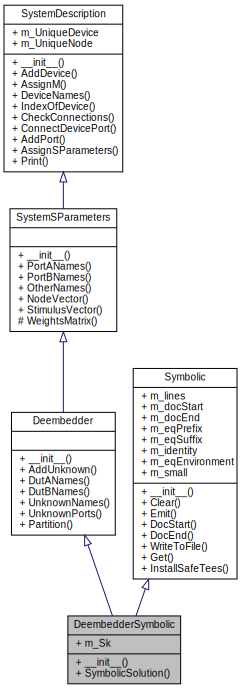
\includegraphics[height=550pt]{classSignalIntegrity_1_1SystemDescriptions_1_1DeembedderSymbolic_1_1DeembedderSymbolic__inherit__graph}
\end{center}
\end{figure}


Collaboration diagram for Deembedder\+Symbolic\+:
\nopagebreak
\begin{figure}[H]
\begin{center}
\leavevmode
\includegraphics[height=550pt]{classSignalIntegrity_1_1SystemDescriptions_1_1DeembedderSymbolic_1_1DeembedderSymbolic__coll__graph}
\end{center}
\end{figure}
\subsection*{Public Member Functions}
\begin{DoxyCompactItemize}
\item 
def \hyperlink{classSignalIntegrity_1_1SystemDescriptions_1_1DeembedderSymbolic_1_1DeembedderSymbolic_a72fa31992e716f60779f561f6cdbb4ce}{\+\_\+\+\_\+init\+\_\+\+\_\+} (self, sd=None, args)
\begin{DoxyCompactList}\small\item\em Constructor. \end{DoxyCompactList}\item 
def \hyperlink{classSignalIntegrity_1_1SystemDescriptions_1_1DeembedderSymbolic_1_1DeembedderSymbolic_a10ef812418fff67deff1540435a9698c}{Symbolic\+Solution} (self)
\begin{DoxyCompactList}\small\item\em Generates a symbolic solution to a deembedding problem described in a \hyperlink{namespaceSignalIntegrity_1_1SystemDescriptions_1_1Deembedder}{Deembedder} class. \end{DoxyCompactList}\end{DoxyCompactItemize}
\subsection*{Additional Inherited Members}


\subsection{Detailed Description}
class for producing symbolic solutions to deembedding problems. 

Definition at line 30 of file Deembedder\+Symbolic.\+py.



\subsection{Constructor \& Destructor Documentation}
\mbox{\Hypertarget{classSignalIntegrity_1_1SystemDescriptions_1_1DeembedderSymbolic_1_1DeembedderSymbolic_a72fa31992e716f60779f561f6cdbb4ce}\label{classSignalIntegrity_1_1SystemDescriptions_1_1DeembedderSymbolic_1_1DeembedderSymbolic_a72fa31992e716f60779f561f6cdbb4ce}} 
\index{Signal\+Integrity\+::\+System\+Descriptions\+::\+Deembedder\+Symbolic\+::\+Deembedder\+Symbolic@{Signal\+Integrity\+::\+System\+Descriptions\+::\+Deembedder\+Symbolic\+::\+Deembedder\+Symbolic}!\+\_\+\+\_\+init\+\_\+\+\_\+@{\+\_\+\+\_\+init\+\_\+\+\_\+}}
\index{\+\_\+\+\_\+init\+\_\+\+\_\+@{\+\_\+\+\_\+init\+\_\+\+\_\+}!Signal\+Integrity\+::\+System\+Descriptions\+::\+Deembedder\+Symbolic\+::\+Deembedder\+Symbolic@{Signal\+Integrity\+::\+System\+Descriptions\+::\+Deembedder\+Symbolic\+::\+Deembedder\+Symbolic}}
\subsubsection{\texorpdfstring{\+\_\+\+\_\+init\+\_\+\+\_\+()}{\_\_init\_\_()}}
{\footnotesize\ttfamily def \+\_\+\+\_\+init\+\_\+\+\_\+ (\begin{DoxyParamCaption}\item[{}]{self,  }\item[{}]{sd = {\ttfamily None},  }\item[{}]{args }\end{DoxyParamCaption})}



Constructor. 


\begin{DoxyParams}{Parameters}
{\em sd} & (optional) instance of class \hyperlink{namespaceSignalIntegrity_1_1SystemDescriptions_1_1SystemDescription}{System\+Description} \\
\hline
{\em args} & (optional) named arguments (name = value)\\
\hline
\end{DoxyParams}
Named arguments passed to the \hyperlink{namespaceSignalIntegrity_1_1SystemDescriptions_1_1Symbolic}{Symbolic} class

\begin{DoxySeeAlso}{See also}
\hyperlink{namespaceSignalIntegrity_1_1SystemDescriptions_1_1Symbolic}{Symbolic} 
\end{DoxySeeAlso}


Definition at line 41 of file Deembedder\+Symbolic.\+py.



\subsection{Member Function Documentation}
\mbox{\Hypertarget{classSignalIntegrity_1_1SystemDescriptions_1_1DeembedderSymbolic_1_1DeembedderSymbolic_a10ef812418fff67deff1540435a9698c}\label{classSignalIntegrity_1_1SystemDescriptions_1_1DeembedderSymbolic_1_1DeembedderSymbolic_a10ef812418fff67deff1540435a9698c}} 
\index{Signal\+Integrity\+::\+System\+Descriptions\+::\+Deembedder\+Symbolic\+::\+Deembedder\+Symbolic@{Signal\+Integrity\+::\+System\+Descriptions\+::\+Deembedder\+Symbolic\+::\+Deembedder\+Symbolic}!Symbolic\+Solution@{Symbolic\+Solution}}
\index{Symbolic\+Solution@{Symbolic\+Solution}!Signal\+Integrity\+::\+System\+Descriptions\+::\+Deembedder\+Symbolic\+::\+Deembedder\+Symbolic@{Signal\+Integrity\+::\+System\+Descriptions\+::\+Deembedder\+Symbolic\+::\+Deembedder\+Symbolic}}
\subsubsection{\texorpdfstring{Symbolic\+Solution()}{SymbolicSolution()}}
{\footnotesize\ttfamily def Symbolic\+Solution (\begin{DoxyParamCaption}\item[{}]{self }\end{DoxyParamCaption})}



Generates a symbolic solution to a deembedding problem described in a \hyperlink{namespaceSignalIntegrity_1_1SystemDescriptions_1_1Deembedder}{Deembedder} class. 

\begin{DoxyReturn}{Returns}
self
\end{DoxyReturn}
The solution is held in the \hyperlink{namespaceSignalIntegrity_1_1SystemDescriptions_1_1Symbolic}{Symbolic} class.

\begin{DoxySeeAlso}{See also}
\hyperlink{namespaceSignalIntegrity_1_1SystemDescriptions_1_1Symbolic}{Symbolic} 
\end{DoxySeeAlso}


Definition at line 55 of file Deembedder\+Symbolic.\+py.



The documentation for this class was generated from the following file\+:\begin{DoxyCompactItemize}
\item 
Py\+S\+I/\+Signal\+Integrity/\+System\+Descriptions/Deembedder\+Symbolic.\+py\end{DoxyCompactItemize}

\hypertarget{classSignalIntegrity_1_1SystemDescriptions_1_1Device_1_1Device}{}\section{Device Class Reference}
\label{classSignalIntegrity_1_1SystemDescriptions_1_1Device_1_1Device}\index{Device@{Device}}


device in system descriptions  




Inherits list.



Collaboration diagram for Device\+:\nopagebreak
\begin{figure}[H]
\begin{center}
\leavevmode
\includegraphics[width=199pt]{classSignalIntegrity_1_1SystemDescriptions_1_1Device_1_1Device__coll__graph}
\end{center}
\end{figure}
\subsection*{Public Member Functions}
\begin{DoxyCompactItemize}
\item 
def \hyperlink{classSignalIntegrity_1_1SystemDescriptions_1_1Device_1_1Device_aa13732b8be1d26511f983436259d282f}{\+\_\+\+\_\+init\+\_\+\+\_\+} (self, Name, Ports, Type=\textquotesingle{}device\textquotesingle{})
\begin{DoxyCompactList}\small\item\em Constructor. \end{DoxyCompactList}\item 
def \hyperlink{classSignalIntegrity_1_1SystemDescriptions_1_1Device_1_1Device_ac588a4be7e9067cb86aed0fc706f4902}{Assign\+S\+Parameters} (self, S\+Parameters)
\begin{DoxyCompactList}\small\item\em assign s-\/parameters to the device \end{DoxyCompactList}\item 
def \hyperlink{classSignalIntegrity_1_1SystemDescriptions_1_1Device_1_1Device_a891ce4dff358dfe4f73c3c0e269bcffd}{Print} (self, level=0)
\begin{DoxyCompactList}\small\item\em print an ascii description of the device \end{DoxyCompactList}\end{DoxyCompactItemize}
\subsection*{Static Public Member Functions}
\begin{DoxyCompactItemize}
\item 
def \hyperlink{classSignalIntegrity_1_1SystemDescriptions_1_1Device_1_1Device_a2c70eb13042897e97cc142e6a0f69300}{Symbolic\+Matrix} (Name, Rows, Columns=-\/1)
\begin{DoxyCompactList}\small\item\em creates a symbolic matrix \end{DoxyCompactList}\end{DoxyCompactItemize}


\subsection{Detailed Description}
device in system descriptions 

a device is fundamentally a list of ports 

Definition at line 18 of file Device.\+py.



\subsection{Constructor \& Destructor Documentation}
\mbox{\Hypertarget{classSignalIntegrity_1_1SystemDescriptions_1_1Device_1_1Device_aa13732b8be1d26511f983436259d282f}\label{classSignalIntegrity_1_1SystemDescriptions_1_1Device_1_1Device_aa13732b8be1d26511f983436259d282f}} 
\index{Signal\+Integrity\+::\+System\+Descriptions\+::\+Device\+::\+Device@{Signal\+Integrity\+::\+System\+Descriptions\+::\+Device\+::\+Device}!\+\_\+\+\_\+init\+\_\+\+\_\+@{\+\_\+\+\_\+init\+\_\+\+\_\+}}
\index{\+\_\+\+\_\+init\+\_\+\+\_\+@{\+\_\+\+\_\+init\+\_\+\+\_\+}!Signal\+Integrity\+::\+System\+Descriptions\+::\+Device\+::\+Device@{Signal\+Integrity\+::\+System\+Descriptions\+::\+Device\+::\+Device}}
\subsubsection{\texorpdfstring{\+\_\+\+\_\+init\+\_\+\+\_\+()}{\_\_init\_\_()}}
{\footnotesize\ttfamily def \+\_\+\+\_\+init\+\_\+\+\_\+ (\begin{DoxyParamCaption}\item[{}]{self,  }\item[{}]{Name,  }\item[{}]{Ports,  }\item[{}]{Type = {\ttfamily \textquotesingle{}device\textquotesingle{}} }\end{DoxyParamCaption})}



Constructor. 


\begin{DoxyParams}{Parameters}
{\em Name} & string unique name of device \\
\hline
{\em Ports} & integer number of ports in device \\
\hline
{\em Type} & (optional) string type of device \\
\hline
\end{DoxyParams}
\begin{DoxyNote}{Note}
valid types of devices are\+:
\begin{DoxyItemize}
\item \textquotesingle{}device\textquotesingle{} -\/ a normal device in a system description.
\item \textquotesingle{}unknown\textquotesingle{} -\/ a device whose s-\/parameters are unknown used in a deembedding solution. 
\end{DoxyItemize}
\end{DoxyNote}


Definition at line 29 of file Device.\+py.



\subsection{Member Function Documentation}
\mbox{\Hypertarget{classSignalIntegrity_1_1SystemDescriptions_1_1Device_1_1Device_ac588a4be7e9067cb86aed0fc706f4902}\label{classSignalIntegrity_1_1SystemDescriptions_1_1Device_1_1Device_ac588a4be7e9067cb86aed0fc706f4902}} 
\index{Signal\+Integrity\+::\+System\+Descriptions\+::\+Device\+::\+Device@{Signal\+Integrity\+::\+System\+Descriptions\+::\+Device\+::\+Device}!Assign\+S\+Parameters@{Assign\+S\+Parameters}}
\index{Assign\+S\+Parameters@{Assign\+S\+Parameters}!Signal\+Integrity\+::\+System\+Descriptions\+::\+Device\+::\+Device@{Signal\+Integrity\+::\+System\+Descriptions\+::\+Device\+::\+Device}}
\subsubsection{\texorpdfstring{Assign\+S\+Parameters()}{AssignSParameters()}}
{\footnotesize\ttfamily def Assign\+S\+Parameters (\begin{DoxyParamCaption}\item[{}]{self,  }\item[{}]{S\+Parameters }\end{DoxyParamCaption})}



assign s-\/parameters to the device 


\begin{DoxyParams}{Parameters}
{\em \hyperlink{namespaceSignalIntegrity_1_1SParameters}{S\+Parameters}} & list of list s-\/parameter matrix \\
\hline
\end{DoxyParams}
\begin{DoxyNote}{Note}
\hyperlink{namespaceSignalIntegrity_1_1SParameters}{S\+Parameters} can be either list of list of complex numbers for numeric solutions or list of list of strings for symbolic solutions. Strings can be La\+TeX strings. 
\end{DoxyNote}


Definition at line 41 of file Device.\+py.

\mbox{\Hypertarget{classSignalIntegrity_1_1SystemDescriptions_1_1Device_1_1Device_a891ce4dff358dfe4f73c3c0e269bcffd}\label{classSignalIntegrity_1_1SystemDescriptions_1_1Device_1_1Device_a891ce4dff358dfe4f73c3c0e269bcffd}} 
\index{Signal\+Integrity\+::\+System\+Descriptions\+::\+Device\+::\+Device@{Signal\+Integrity\+::\+System\+Descriptions\+::\+Device\+::\+Device}!Print@{Print}}
\index{Print@{Print}!Signal\+Integrity\+::\+System\+Descriptions\+::\+Device\+::\+Device@{Signal\+Integrity\+::\+System\+Descriptions\+::\+Device\+::\+Device}}
\subsubsection{\texorpdfstring{Print()}{Print()}}
{\footnotesize\ttfamily def Print (\begin{DoxyParamCaption}\item[{}]{self,  }\item[{}]{level = {\ttfamily 0} }\end{DoxyParamCaption})}



print an ascii description of the device 


\begin{DoxyParams}{Parameters}
{\em level} & (optional) level to print at. This affects the indentation. when called to just print a device, use the default argument, otherwise, when it\textquotesingle{}s printed by printing a system description, it will be indented for each device. \\
\hline
\end{DoxyParams}


Definition at line 76 of file Device.\+py.

\mbox{\Hypertarget{classSignalIntegrity_1_1SystemDescriptions_1_1Device_1_1Device_a2c70eb13042897e97cc142e6a0f69300}\label{classSignalIntegrity_1_1SystemDescriptions_1_1Device_1_1Device_a2c70eb13042897e97cc142e6a0f69300}} 
\index{Signal\+Integrity\+::\+System\+Descriptions\+::\+Device\+::\+Device@{Signal\+Integrity\+::\+System\+Descriptions\+::\+Device\+::\+Device}!Symbolic\+Matrix@{Symbolic\+Matrix}}
\index{Symbolic\+Matrix@{Symbolic\+Matrix}!Signal\+Integrity\+::\+System\+Descriptions\+::\+Device\+::\+Device@{Signal\+Integrity\+::\+System\+Descriptions\+::\+Device\+::\+Device}}
\subsubsection{\texorpdfstring{Symbolic\+Matrix()}{SymbolicMatrix()}}
{\footnotesize\ttfamily def Symbolic\+Matrix (\begin{DoxyParamCaption}\item[{}]{Name,  }\item[{}]{Rows,  }\item[{}]{Columns = {\ttfamily -\/1} }\end{DoxyParamCaption})\hspace{0.3cm}{\ttfamily [static]}}



creates a symbolic matrix 

The matrix is of a simple form. It is a list of list of strings where the string is either\+:
\begin{DoxyItemize}
\item rows=columns=1 -\/ \mbox{[}\mbox{[}name\mbox{]}\mbox{]}
\item rows $<$= 9 and columns $<$= 9 -\/ list of list of name+\textquotesingle{}\+\_\+\textquotesingle{}+str(r+1)+str(c+1) \begin{DoxyNote}{Note}
if a row or column goes above 9, a comma is inserted between the port numbers to remove ambiguity. 
\end{DoxyNote}

\begin{DoxyParams}{Parameters}
{\em Name} & string name of device \\
\hline
{\em Rows} & integer number of rows in the matrix \\
\hline
{\em Columns} & (optional) integer number of columns in the matrix (defaults to the number of rows). \\
\hline
\end{DoxyParams}

\end{DoxyItemize}

Definition at line 62 of file Device.\+py.



The documentation for this class was generated from the following file\+:\begin{DoxyCompactItemize}
\item 
Py\+S\+I/\+Signal\+Integrity/\+System\+Descriptions/Device.\+py\end{DoxyCompactItemize}

\hypertarget{classSignalIntegrity_1_1Parsers_1_1Devices_1_1DeviceParser_1_1DeviceFactory}{}\section{Device\+Factory Class Reference}
\label{classSignalIntegrity_1_1Parsers_1_1Devices_1_1DeviceParser_1_1DeviceFactory}\index{Device\+Factory@{Device\+Factory}}


device class factory that produces devices  




Inherits list.



Collaboration diagram for Device\+Factory\+:\nopagebreak
\begin{figure}[H]
\begin{center}
\leavevmode
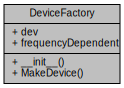
\includegraphics[width=196pt]{classSignalIntegrity_1_1Parsers_1_1Devices_1_1DeviceParser_1_1DeviceFactory__coll__graph}
\end{center}
\end{figure}
\subsection*{Public Member Functions}
\begin{DoxyCompactItemize}
\item 
def \hyperlink{classSignalIntegrity_1_1Parsers_1_1Devices_1_1DeviceParser_1_1DeviceFactory_ae64f0875afe3067b97ba370b354b9213}{\+\_\+\+\_\+init\+\_\+\+\_\+} (self)
\begin{DoxyCompactList}\small\item\em Constructor. \end{DoxyCompactList}\item 
def \hyperlink{classSignalIntegrity_1_1Parsers_1_1Devices_1_1DeviceParser_1_1DeviceFactory_a84bd6828768b3a1677c71d39f3cb91dd}{Make\+Device} (self, ports, args\+List, f)
\begin{DoxyCompactList}\small\item\em makes a device from a set of arguments \end{DoxyCompactList}\end{DoxyCompactItemize}
\subsection*{Public Attributes}
\begin{DoxyCompactItemize}
\item 
\mbox{\Hypertarget{classSignalIntegrity_1_1Parsers_1_1Devices_1_1DeviceParser_1_1DeviceFactory_ac43812121e594f158520698ba706118f}\label{classSignalIntegrity_1_1Parsers_1_1Devices_1_1DeviceParser_1_1DeviceFactory_ac43812121e594f158520698ba706118f}} 
\hyperlink{classSignalIntegrity_1_1Parsers_1_1Devices_1_1DeviceParser_1_1DeviceFactory_ac43812121e594f158520698ba706118f}{dev}
\begin{DoxyCompactList}\small\item\em instance of class \hyperlink{namespaceSignalIntegrity_1_1SParameters}{S\+Parameters} or list of list matrix when not frequency dependent. \end{DoxyCompactList}\item 
\hyperlink{classSignalIntegrity_1_1Parsers_1_1Devices_1_1DeviceParser_1_1DeviceFactory_a3909d31bcdbe6e7a3450d1fa216755a2}{frequency\+Dependent}
\begin{DoxyCompactList}\small\item\em boolean whether dev is frequency dependent. \end{DoxyCompactList}\end{DoxyCompactItemize}


\subsection{Detailed Description}
device class factory that produces devices 

Definition at line 43 of file Device\+Parser.\+py.



\subsection{Constructor \& Destructor Documentation}
\mbox{\Hypertarget{classSignalIntegrity_1_1Parsers_1_1Devices_1_1DeviceParser_1_1DeviceFactory_ae64f0875afe3067b97ba370b354b9213}\label{classSignalIntegrity_1_1Parsers_1_1Devices_1_1DeviceParser_1_1DeviceFactory_ae64f0875afe3067b97ba370b354b9213}} 
\index{Signal\+Integrity\+::\+Parsers\+::\+Devices\+::\+Device\+Parser\+::\+Device\+Factory@{Signal\+Integrity\+::\+Parsers\+::\+Devices\+::\+Device\+Parser\+::\+Device\+Factory}!\+\_\+\+\_\+init\+\_\+\+\_\+@{\+\_\+\+\_\+init\+\_\+\+\_\+}}
\index{\+\_\+\+\_\+init\+\_\+\+\_\+@{\+\_\+\+\_\+init\+\_\+\+\_\+}!Signal\+Integrity\+::\+Parsers\+::\+Devices\+::\+Device\+Parser\+::\+Device\+Factory@{Signal\+Integrity\+::\+Parsers\+::\+Devices\+::\+Device\+Parser\+::\+Device\+Factory}}
\subsubsection{\texorpdfstring{\+\_\+\+\_\+init\+\_\+\+\_\+()}{\_\_init\_\_()}}
{\footnotesize\ttfamily def \+\_\+\+\_\+init\+\_\+\+\_\+ (\begin{DoxyParamCaption}\item[{}]{self }\end{DoxyParamCaption})}



Constructor. 

list of devices

\tabulinesep=1mm
\begin{longtabu} spread 0pt [c]{*{6}{|X[-1]}|}
\hline
\rowcolor{\tableheadbgcolor}\PBS\centering \textbf{ name }&\PBS\centering \textbf{ ports}&\PBS\centering \textbf{ arginname}&\PBS\centering \textbf{ defaults }&\PBS\centering \textbf{ frequency~\newline
 dependent}&\textbf{ device  }\\\cline{1-6}
\endfirsthead
\hline
\endfoot
\hline
\rowcolor{\tableheadbgcolor}\PBS\centering \textbf{ name }&\PBS\centering \textbf{ ports}&\PBS\centering \textbf{ arginname}&\PBS\centering \textbf{ defaults }&\PBS\centering \textbf{ frequency~\newline
 dependent}&\textbf{ device  }\\\cline{1-6}
\endhead
\PBS\centering file &\PBS\centering any &\PBS\centering True &\PBS\centering filename=None &\PBS\centering True &sp.\+dev.\+S\+Parameter\+File(filename,50.) \\\cline{1-6}
\PBS\centering c &\PBS\centering 1 &\PBS\centering True &\PBS\centering c=None df=0 esr=0 z0=50 &\PBS\centering True &sp.\+dev.\+Termination\+C(f,c,z0,df,esr) \\\cline{1-6}
\PBS\centering c &\PBS\centering 2 &\PBS\centering True &\PBS\centering c=None df=0 esr=0 z0=50 &\PBS\centering True &sp.\+dev.\+Series\+C(f,c,z0,df,esr) \\\cline{1-6}
\PBS\centering l &\PBS\centering 1 &\PBS\centering True &\PBS\centering l=None &\PBS\centering True &sp.\+dev.\+Termination\+L(f,l,z0) \\\cline{1-6}
\PBS\centering l &\PBS\centering 2 &\PBS\centering True &\PBS\centering l=None &\PBS\centering True &sp.\+dev.\+Series\+L(f,l,z0) \\\cline{1-6}
\PBS\centering r &\PBS\centering 1 &\PBS\centering True &\PBS\centering r=None &\PBS\centering False &dev.\+Termination\+Z(r) \\\cline{1-6}
\PBS\centering r &\PBS\centering 2 &\PBS\centering True &\PBS\centering r=None &\PBS\centering False &dev.\+Series\+Z(r) \\\cline{1-6}
\PBS\centering rse &\PBS\centering 2 &\PBS\centering True &\PBS\centering r=None &\PBS\centering True &sp.\+dev.\+Series\+Rse(r) \\\cline{1-6}
\PBS\centering shunt &\PBS\centering 2-\/4 &\PBS\centering True &\PBS\centering r=None &\PBS\centering False &dev.\+Shunt\+Z(ports,r) \\\cline{1-6}
\PBS\centering m &\PBS\centering 4 &\PBS\centering True &\PBS\centering m=None &\PBS\centering True &sp.\+dev.\+Mutual(f,m) \\\cline{1-6}
\PBS\centering ground &\PBS\centering 1 &\PBS\centering False &\PBS\centering &\PBS\centering False &dev.\+Ground() \\\cline{1-6}
\PBS\centering open &\PBS\centering 1 &\PBS\centering False &\PBS\centering &\PBS\centering False &dev.\+Open() \\\cline{1-6}
\PBS\centering thru &\PBS\centering 2 &\PBS\centering False &\PBS\centering &\PBS\centering False &dev.\+Thru() \\\cline{1-6}
\PBS\centering directional~\newline
 coupler &\PBS\centering 3-\/4 &\PBS\centering False &\PBS\centering &\PBS\centering False &dev.\+Directional\+Coupler(ports) \\\cline{1-6}
\PBS\centering termination &\PBS\centering any &\PBS\centering False &\PBS\centering &\PBS\centering False &zeros(shape=(ports,ports)).tolist() \\\cline{1-6}
\PBS\centering tee &\PBS\centering any &\PBS\centering False &\PBS\centering &\PBS\centering False &dev.\+Tee(ports) \\\cline{1-6}
\PBS\centering mixedmode &\PBS\centering 4 &\PBS\centering True &\PBS\centering \textquotesingle{}power\textquotesingle{} &\PBS\centering False &dev.\+Mixed\+Mode\+Converter()~\newline
 or dev.\+Mixed\+Mode\+Converter\+Voltage() \\\cline{1-6}
\PBS\centering ideal~\newline
 transformer &\PBS\centering 4 &\PBS\centering True &\PBS\centering tr=1 &\PBS\centering False &dev.\+Ideal\+Transformer(tr) \\\cline{1-6}
\PBS\centering voltage~\newline
 controlled~\newline
 voltage~\newline
 source&\PBS\centering 4 &\PBS\centering True &\PBS\centering gain=None &\PBS\centering False &dev.\+Voltage\+Controlled\+Voltage\+Source(gain) \\\cline{1-6}
\PBS\centering current~\newline
 controlled~\newline
 current~\newline
 source&\PBS\centering 4 &\PBS\centering True &\PBS\centering gain=None &\PBS\centering False &dev.\+Current\+Controlled\+Current\+Source(gain) \\\cline{1-6}
\PBS\centering current~\newline
 controlled~\newline
 voltage~\newline
 source&\PBS\centering 4 &\PBS\centering True &\PBS\centering gain=None &\PBS\centering False &dev.\+Current\+Controlled\+Voltage\+Source(gain) \\\cline{1-6}
\PBS\centering voltage~\newline
 controlled~\newline
 current~\newline
 source&\PBS\centering 4 &\PBS\centering True &\PBS\centering gain=None &\PBS\centering False &dev.\+Voltage\+Controlled\+Current\+Source(gain) \\\cline{1-6}
\PBS\centering voltage~\newline
 amplifier &\PBS\centering 2-\/4 &\PBS\centering False &\PBS\centering gain=None zo=0 zi=1e8 z0=50 &\PBS\centering False &dev.\+Voltage\+Amplifier(ports,gain,zi,zo) \\\cline{1-6}
\PBS\centering current~\newline
 amplifier &\PBS\centering 2-\/4 &\PBS\centering False &\PBS\centering gain=None zo=1e8 zi=0 z0=50 &\PBS\centering False &dev.\+Current\+Amplifier(ports,gain,zi,zo) \\\cline{1-6}
\PBS\centering transresistance~\newline
 amplifier &\PBS\centering 2-\/4 &\PBS\centering False &\PBS\centering gain=None zo=0 zi=0 z0=50 &\PBS\centering False &dev.\+Transresistance\+Amplifier(ports,gain,zi,zo) \\\cline{1-6}
\PBS\centering transconductance~\newline
 amplifier &\PBS\centering 2-\/4 &\PBS\centering False &\PBS\centering gain=None zo=1e8 zi=1e8 z0=50 &\PBS\centering False &dev.\+Transconductance\+Amplifier(ports,gain,zi,zo) \\\cline{1-6}
\PBS\centering opamp &\PBS\centering 3 &\PBS\centering False &\PBS\centering zi=1e8 zd=1e8 zo=0 gain=1e8 z0=50 &\PBS\centering False &dev.\+Operational\+Amplifier(zi,zd,zo,gain,z0) \\\cline{1-6}
\PBS\centering tline &\PBS\centering 2,4 &\PBS\centering False &\PBS\centering zc=50 td=0 &\PBS\centering True &sp.\+dev.\+T\+Line\+Lossless(f,ports,zc,td) \\\cline{1-6}
\PBS\centering telegrapher &\PBS\centering 2 &\PBS\centering False &\PBS\centering r=0 rse=0 l=0 c=0 df=0 g=0 z0=50 sect=0 &\PBS\centering True &sp.\+dev.\+T\+Line\+Two\+Port\+R\+L\+GC(~\newline
 f,r,rse,l,g,c,df,z0,sect) \\\cline{1-6}
\PBS\centering telegrapher &\PBS\centering 4 &\PBS\centering False &\PBS\centering rp=0 rsep=0 lp=0 cp=0~\newline
 dfp=0 gp=0 rn=0 rsen=0~\newline
 ln=0 cn=0 dfn=0 gn=0~\newline
 lm 0 gm=0 z0=50 sect=0 &\PBS\centering True &sp.\+dev.\+T\+Line\+Differential\+R\+L\+GC(~\newline
 f,rp,rsep,lp,gp,cp,dfp,~\newline
 rn,rsen,ln,gn,cn,dfn,~\newline
 cm,dfm,gm,lm,z0,sect) \\\cline{1-6}
\PBS\centering shortstd &\PBS\centering 1 &\PBS\centering False &\PBS\centering od=0 oz0=50 ol=0 l0=0~\newline
 l1=0.\+0 l2=0 l3=0 &\PBS\centering True &m.\+calkit.\+std.\+Short\+Standard(f,od,oz0,ol,l0,l1,l2,l3) \\\cline{1-6}
\PBS\centering openstd &\PBS\centering 1 &\PBS\centering False &\PBS\centering od=0 oz0=50 ol=0 c0=0~\newline
 c1=0 c2=0 c3=0 &\PBS\centering True &m.\+calkit.\+std.\+Open\+Standard(f,od,oz0,ol,c0,c1,c2,c3) \\\cline{1-6}
\PBS\centering loadstd &\PBS\centering 1 &\PBS\centering False &\PBS\centering od=0 oz0=50 ol=0 tz0=50 &\PBS\centering True &m.\+calkit.\+std.\+Load\+Standard(f,od,oz0,ol,tz0) \\\cline{1-6}
\PBS\centering thrustd &\PBS\centering 2 &\PBS\centering False &\PBS\centering od=0 oz0=50 ol=0 &\PBS\centering True &m.\+calkit.\+std.\+Thru\+Standard(f,od,oz0,ol) \\\cline{1-6}
\end{longtabu}
\begin{DoxyNote}{Note}
ports any mean None supplied. comma or dash separated ports are supplied as a string. 

arginname means the argument is supplied without a keyword. The first default argument has the actual name of the argument. 

frequency dependent devices usually come from \textquotesingle{}sp.\+dev\textquotesingle{} meaning \hyperlink{namespaceSignalIntegrity_1_1SParameters_1_1Devices}{S\+Parameters.\+Devices} package. \hyperlink{namespaceSignalIntegrity_1_1Parsers_1_1Devices}{Devices} that are not frequency dependent come from \textquotesingle{}dev\textquotesingle{} meaning devices. \textquotesingle{}m.\+calkit.\+std\textquotesingle{} refers to \textquotesingle{}\hyperlink{namespaceSignalIntegrity_1_1Measurement_1_1CalKit_1_1Standards}{Measurement.\+Cal\+Kit.\+Standards}\textquotesingle{} package. 

Usually when an argument is defaulted to None, the device production will fail if the argument is not supplied -\/ meaning the default value cannot be used. 
\end{DoxyNote}


Definition at line 92 of file Device\+Parser.\+py.



\subsection{Member Function Documentation}
\mbox{\Hypertarget{classSignalIntegrity_1_1Parsers_1_1Devices_1_1DeviceParser_1_1DeviceFactory_a84bd6828768b3a1677c71d39f3cb91dd}\label{classSignalIntegrity_1_1Parsers_1_1Devices_1_1DeviceParser_1_1DeviceFactory_a84bd6828768b3a1677c71d39f3cb91dd}} 
\index{Signal\+Integrity\+::\+Parsers\+::\+Devices\+::\+Device\+Parser\+::\+Device\+Factory@{Signal\+Integrity\+::\+Parsers\+::\+Devices\+::\+Device\+Parser\+::\+Device\+Factory}!Make\+Device@{Make\+Device}}
\index{Make\+Device@{Make\+Device}!Signal\+Integrity\+::\+Parsers\+::\+Devices\+::\+Device\+Parser\+::\+Device\+Factory@{Signal\+Integrity\+::\+Parsers\+::\+Devices\+::\+Device\+Parser\+::\+Device\+Factory}}
\subsubsection{\texorpdfstring{Make\+Device()}{MakeDevice()}}
{\footnotesize\ttfamily def Make\+Device (\begin{DoxyParamCaption}\item[{}]{self,  }\item[{}]{ports,  }\item[{}]{args\+List,  }\item[{}]{f }\end{DoxyParamCaption})}



makes a device from a set of arguments 

The device is assigned to self.\+dev and self.\+frequency\+Dependent determines whether the device is frequency dependent. Frequency dependent devices are assumed to be instances of the class \hyperlink{namespaceSignalIntegrity_1_1SParameters}{S\+Parameters}. Otherwise, they are list of list matrices.


\begin{DoxyParams}{Parameters}
{\em ports} & integer number of ports \\
\hline
{\em args\+List} & list of arguments. The name of the device is the first argument. If the device has no keyword for the argument, then that argument is next. Otherwise, besides the name and the argument with no keyword, the remaining arguments come in keyword/value pairs where the keyword is a string and the value is the value of the keyword. \\
\hline
{\em f} & list of frequencies \\
\hline
\end{DoxyParams}
\begin{DoxyReturn}{Returns}
boolean whether the device was created. 
\end{DoxyReturn}

\begin{DoxyExceptions}{Exceptions}
{\em Py\+S\+I\+Exception\+Device\+Parser} & if the device cannot be created. \\
\hline
\end{DoxyExceptions}


Definition at line 195 of file Device\+Parser.\+py.



\subsection{Member Data Documentation}
\mbox{\Hypertarget{classSignalIntegrity_1_1Parsers_1_1Devices_1_1DeviceParser_1_1DeviceFactory_a3909d31bcdbe6e7a3450d1fa216755a2}\label{classSignalIntegrity_1_1Parsers_1_1Devices_1_1DeviceParser_1_1DeviceFactory_a3909d31bcdbe6e7a3450d1fa216755a2}} 
\index{Signal\+Integrity\+::\+Parsers\+::\+Devices\+::\+Device\+Parser\+::\+Device\+Factory@{Signal\+Integrity\+::\+Parsers\+::\+Devices\+::\+Device\+Parser\+::\+Device\+Factory}!frequency\+Dependent@{frequency\+Dependent}}
\index{frequency\+Dependent@{frequency\+Dependent}!Signal\+Integrity\+::\+Parsers\+::\+Devices\+::\+Device\+Parser\+::\+Device\+Factory@{Signal\+Integrity\+::\+Parsers\+::\+Devices\+::\+Device\+Parser\+::\+Device\+Factory}}
\subsubsection{\texorpdfstring{frequency\+Dependent}{frequencyDependent}}
{\footnotesize\ttfamily frequency\+Dependent}



boolean whether dev is frequency dependent. 

pragma\+: include 

Definition at line 290 of file Device\+Parser.\+py.



The documentation for this class was generated from the following file\+:\begin{DoxyCompactItemize}
\item 
Py\+S\+I/\+Signal\+Integrity/\+Parsers/\+Devices/Device\+Parser.\+py\end{DoxyCompactItemize}

\hypertarget{classSignalIntegrity_1_1Parsers_1_1Devices_1_1DeviceParser_1_1DeviceParser}{}\section{Device\+Parser Class Reference}
\label{classSignalIntegrity_1_1Parsers_1_1Devices_1_1DeviceParser_1_1DeviceParser}\index{Device\+Parser@{Device\+Parser}}


contains s-\/parameters of devices made from a netlist line  




Collaboration diagram for Device\+Parser\+:
\nopagebreak
\begin{figure}[H]
\begin{center}
\leavevmode
\includegraphics[width=167pt]{classSignalIntegrity_1_1Parsers_1_1Devices_1_1DeviceParser_1_1DeviceParser__coll__graph}
\end{center}
\end{figure}
\subsection*{Public Member Functions}
\begin{DoxyCompactItemize}
\item 
def \hyperlink{classSignalIntegrity_1_1Parsers_1_1Devices_1_1DeviceParser_1_1DeviceParser_a286a7f15e5aa7761d219f91accd234c1}{\+\_\+\+\_\+init\+\_\+\+\_\+} (self, f, ports, args\+List)
\begin{DoxyCompactList}\small\item\em Constructor. \end{DoxyCompactList}\end{DoxyCompactItemize}
\subsection*{Public Attributes}
\begin{DoxyCompactItemize}
\item 
\mbox{\Hypertarget{classSignalIntegrity_1_1Parsers_1_1Devices_1_1DeviceParser_1_1DeviceParser_a40a26fb5046a51e40dd1b61c78d72ace}\label{classSignalIntegrity_1_1Parsers_1_1Devices_1_1DeviceParser_1_1DeviceParser_a40a26fb5046a51e40dd1b61c78d72ace}} 
\hyperlink{classSignalIntegrity_1_1Parsers_1_1Devices_1_1DeviceParser_1_1DeviceParser_a40a26fb5046a51e40dd1b61c78d72ace}{m\+\_\+f}
\begin{DoxyCompactList}\small\item\em list of frequencies pragma\+: include \end{DoxyCompactList}\item 
\mbox{\Hypertarget{classSignalIntegrity_1_1Parsers_1_1Devices_1_1DeviceParser_1_1DeviceParser_aeca0e75de33f68cf0f94eb5c932037bd}\label{classSignalIntegrity_1_1Parsers_1_1Devices_1_1DeviceParser_1_1DeviceParser_aeca0e75de33f68cf0f94eb5c932037bd}} 
\hyperlink{classSignalIntegrity_1_1Parsers_1_1Devices_1_1DeviceParser_1_1DeviceParser_aeca0e75de33f68cf0f94eb5c932037bd}{m\+\_\+sp}
\begin{DoxyCompactList}\small\item\em None if device is frequency dependent otherwise an instance of class \hyperlink{namespaceSignalIntegrity_1_1SParameters}{S\+Parameters}. \end{DoxyCompactList}\item 
\mbox{\Hypertarget{classSignalIntegrity_1_1Parsers_1_1Devices_1_1DeviceParser_1_1DeviceParser_a5bad8e400189aa634b24535daee44ee0}\label{classSignalIntegrity_1_1Parsers_1_1Devices_1_1DeviceParser_1_1DeviceParser_a5bad8e400189aa634b24535daee44ee0}} 
\hyperlink{classSignalIntegrity_1_1Parsers_1_1Devices_1_1DeviceParser_1_1DeviceParser_a5bad8e400189aa634b24535daee44ee0}{m\+\_\+spf}
\begin{DoxyCompactList}\small\item\em None if device is not frequency dependent otherwise a list of list s-\/parameter matrix. \end{DoxyCompactList}\end{DoxyCompactItemize}


\subsection{Detailed Description}
contains s-\/parameters of devices made from a netlist line 

Definition at line 316 of file Device\+Parser.\+py.



\subsection{Constructor \& Destructor Documentation}
\mbox{\Hypertarget{classSignalIntegrity_1_1Parsers_1_1Devices_1_1DeviceParser_1_1DeviceParser_a286a7f15e5aa7761d219f91accd234c1}\label{classSignalIntegrity_1_1Parsers_1_1Devices_1_1DeviceParser_1_1DeviceParser_a286a7f15e5aa7761d219f91accd234c1}} 
\index{Signal\+Integrity\+::\+Parsers\+::\+Devices\+::\+Device\+Parser\+::\+Device\+Parser@{Signal\+Integrity\+::\+Parsers\+::\+Devices\+::\+Device\+Parser\+::\+Device\+Parser}!\+\_\+\+\_\+init\+\_\+\+\_\+@{\+\_\+\+\_\+init\+\_\+\+\_\+}}
\index{\+\_\+\+\_\+init\+\_\+\+\_\+@{\+\_\+\+\_\+init\+\_\+\+\_\+}!Signal\+Integrity\+::\+Parsers\+::\+Devices\+::\+Device\+Parser\+::\+Device\+Parser@{Signal\+Integrity\+::\+Parsers\+::\+Devices\+::\+Device\+Parser\+::\+Device\+Parser}}
\subsubsection{\texorpdfstring{\+\_\+\+\_\+init\+\_\+\+\_\+()}{\_\_init\_\_()}}
{\footnotesize\ttfamily def \+\_\+\+\_\+init\+\_\+\+\_\+ (\begin{DoxyParamCaption}\item[{}]{self,  }\item[{}]{f,  }\item[{}]{ports,  }\item[{}]{args\+List }\end{DoxyParamCaption})}



Constructor. 

makes a device from a set of arguments

The device is assigned to self.\+m\+\_\+spf if frequency\+Dependent and assumed to be an instance of class \hyperlink{namespaceSignalIntegrity_1_1SParameters}{S\+Parameters}. Otherwise, it is assigned to self.\+m\+\_\+sp and is assumed to be a list of list matrix.

The intent of this class is that \char`\"{}\+Parser\char`\"{} classes use this \hyperlink{classSignalIntegrity_1_1Parsers_1_1Devices_1_1DeviceParser_1_1DeviceParser}{Device\+Parser} to parse netlist lines that have \textquotesingle{}device\textquotesingle{} as the first token. It keeps these s-\/parameters and assigns them as it loops over the frequencies generating numeric solutions.


\begin{DoxyParams}{Parameters}
{\em f} & list of frequencies \\
\hline
{\em ports} & integer number of ports \\
\hline
{\em args\+List} & list of arguments. The name of the device is the first argument. If the device has no keyword for the argument, then that argument is next. Otherwise, besides the name and the argument with no keyword, the remaining arguments come in keyword/value pairs where the keyword is a string and the value is the value of the keyword. \\
\hline
\end{DoxyParams}
\begin{DoxyReturn}{Returns}
None 
\end{DoxyReturn}

\begin{DoxyExceptions}{Exceptions}
{\em Py\+S\+I\+Exception\+Device\+Parser} & if the device cannot be created. \\
\hline
\end{DoxyExceptions}
\begin{DoxySeeAlso}{See also}
\hyperlink{namespaceSignalIntegrity_1_1Parsers_1_1SystemDescriptionParser}{Signal\+Integrity.\+Parsers.\+System\+Description\+Parser} 
\end{DoxySeeAlso}


Definition at line 346 of file Device\+Parser.\+py.



The documentation for this class was generated from the following file\+:\begin{DoxyCompactItemize}
\item 
Py\+S\+I/\+Signal\+Integrity/\+Parsers/\+Devices/Device\+Parser.\+py\end{DoxyCompactItemize}

\hypertarget{classSignalIntegrity_1_1Measurement_1_1Calibration_1_1ErrorTerms_1_1ErrorTerms}{}\section{Error\+Terms Class Reference}
\label{classSignalIntegrity_1_1Measurement_1_1Calibration_1_1ErrorTerms_1_1ErrorTerms}\index{Error\+Terms@{Error\+Terms}}


Error terms for V\+NA and \hyperlink{namespaceSignalIntegrity_1_1Measurement_1_1TDR}{T\+DR} based s-\/parameter calculations.  




Inherits object.



Collaboration diagram for Error\+Terms\+:
\nopagebreak
\begin{figure}[H]
\begin{center}
\leavevmode
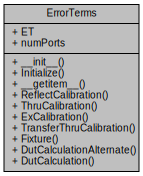
\includegraphics[width=215pt]{classSignalIntegrity_1_1Measurement_1_1Calibration_1_1ErrorTerms_1_1ErrorTerms__coll__graph}
\end{center}
\end{figure}
\subsection*{Public Member Functions}
\begin{DoxyCompactItemize}
\item 
def \hyperlink{classSignalIntegrity_1_1Measurement_1_1Calibration_1_1ErrorTerms_1_1ErrorTerms_ad8cdadc2d29a11c5f69d487c0bf1a7a3}{\+\_\+\+\_\+init\+\_\+\+\_\+} (self, ET=None)
\begin{DoxyCompactList}\small\item\em Constructor. \end{DoxyCompactList}\item 
def \hyperlink{classSignalIntegrity_1_1Measurement_1_1Calibration_1_1ErrorTerms_1_1ErrorTerms_a76b02819f5b0a67b717af159f71f4ca3}{Initialize} (self, num\+Ports)
\begin{DoxyCompactList}\small\item\em Initialize. \end{DoxyCompactList}\item 
def \hyperlink{classSignalIntegrity_1_1Measurement_1_1Calibration_1_1ErrorTerms_1_1ErrorTerms_aab91ae2e037c39b631a69273c277bfe9}{\+\_\+\+\_\+getitem\+\_\+\+\_\+} (self, item)
\begin{DoxyCompactList}\small\item\em overloads \mbox{[}item\mbox{]} \end{DoxyCompactList}\item 
def \hyperlink{classSignalIntegrity_1_1Measurement_1_1Calibration_1_1ErrorTerms_1_1ErrorTerms_afb72282df42e631477c1658bc52a6a91}{Reflect\+Calibration} (self, hat\+Gamma, Gamma, m)
\begin{DoxyCompactList}\small\item\em performs a reflect calibration \end{DoxyCompactList}\item 
def \hyperlink{classSignalIntegrity_1_1Measurement_1_1Calibration_1_1ErrorTerms_1_1ErrorTerms_a06196443ad991bcdaccb2db32f396f00}{Thru\+Calibration} (self, b1a1, b2a1, S, n, m)
\begin{DoxyCompactList}\small\item\em performs a thru calibration \end{DoxyCompactList}\item 
def \hyperlink{classSignalIntegrity_1_1Measurement_1_1Calibration_1_1ErrorTerms_1_1ErrorTerms_a7dd89d542be158c0b13f2c0b7f2a852c}{Ex\+Calibration} (self, b2a1, n, m)
\begin{DoxyCompactList}\small\item\em Computes the crosstalk term. \end{DoxyCompactList}\item 
def \hyperlink{classSignalIntegrity_1_1Measurement_1_1Calibration_1_1ErrorTerms_1_1ErrorTerms_ac22781b57de46a1993aaaf0104cb2331}{Transfer\+Thru\+Calibration} (self)
\begin{DoxyCompactList}\small\item\em Performs the transfer thru calibrations. \end{DoxyCompactList}\item 
def \hyperlink{classSignalIntegrity_1_1Measurement_1_1Calibration_1_1ErrorTerms_1_1ErrorTerms_a7df5e396b9b1e7d1a8ac4d549a729494}{Fixture} (self, m)
\begin{DoxyCompactList}\small\item\em Fixture. \end{DoxyCompactList}\item 
def \hyperlink{classSignalIntegrity_1_1Measurement_1_1Calibration_1_1ErrorTerms_1_1ErrorTerms_aaa197534b553fe80ed41db445147cbc3}{Dut\+Calculation\+Alternate} (self, s\+Raw)
\begin{DoxyCompactList}\small\item\em Alternate Dut Calculation. \end{DoxyCompactList}\item 
def \hyperlink{classSignalIntegrity_1_1Measurement_1_1Calibration_1_1ErrorTerms_1_1ErrorTerms_ac257ff0d436f9c02507349f82ece9e56}{Dut\+Calculation} (self, s\+Raw)
\begin{DoxyCompactList}\small\item\em Calculates a D\+UT. \end{DoxyCompactList}\end{DoxyCompactItemize}


\subsection{Detailed Description}
Error terms for V\+NA and \hyperlink{namespaceSignalIntegrity_1_1Measurement_1_1TDR}{T\+DR} based s-\/parameter calculations. 

Error terms are, for P ports, a P x P matrix of lists of three error terms. For the diagonal elements, the three error terms are ED, ER, and ES in that order for the off diagonal elements, the three error terms are EX, ET and EL in that order for r in 0...P-\/1, and c in 0...P-\/1, ET\mbox{[}r\mbox{]}\mbox{[}c\mbox{]} = \mbox{[}ED\mbox{[}r\mbox{]},ER\mbox{[}r\mbox{]},ES\mbox{[}r\mbox{]}\mbox{]}, when r==c ET\mbox{[}r\mbox{]}\mbox{[}c\mbox{]}=\mbox{[}EX\mbox{[}r\mbox{]}\mbox{[}c\mbox{]},ET\mbox{[}r\mbox{]}\mbox{[}c\mbox{]},EL\mbox{[}r\mbox{]}\mbox{[}c\mbox{]}\mbox{]} when r !=c

ET\mbox{[}r\mbox{]}\mbox{[}c\mbox{]} refers to the error terms at port r when driven at port c in other words, if r==c, then\+: ET\mbox{[}r\mbox{]}\mbox{[}r\mbox{]}\mbox{[}0\mbox{]} = E\+Dr ET\mbox{[}r\mbox{]}\mbox{[}r\mbox{]}\mbox{[}1\mbox{]} = E\+Rr ET\mbox{[}r\mbox{]}\mbox{[}r\mbox{]}\mbox{[}2\mbox{]} = E\+Sr and when r!=c, then\+: ET\mbox{[}r\mbox{]}\mbox{[}c\mbox{]}\mbox{[}0\mbox{]}=E\+Xrc ET\mbox{[}r\mbox{]}\mbox{[}c\mbox{]}\mbox{[}1\mbox{]}=E\+Trc ET\mbox{[}r\mbox{]}\mbox{[}c\mbox{]}\mbox{[}2\mbox{]}=E\+Lrc 

Definition at line 43 of file Error\+Terms.\+py.



\subsection{Constructor \& Destructor Documentation}
\mbox{\Hypertarget{classSignalIntegrity_1_1Measurement_1_1Calibration_1_1ErrorTerms_1_1ErrorTerms_ad8cdadc2d29a11c5f69d487c0bf1a7a3}\label{classSignalIntegrity_1_1Measurement_1_1Calibration_1_1ErrorTerms_1_1ErrorTerms_ad8cdadc2d29a11c5f69d487c0bf1a7a3}} 
\index{Signal\+Integrity\+::\+Measurement\+::\+Calibration\+::\+Error\+Terms\+::\+Error\+Terms@{Signal\+Integrity\+::\+Measurement\+::\+Calibration\+::\+Error\+Terms\+::\+Error\+Terms}!\+\_\+\+\_\+init\+\_\+\+\_\+@{\+\_\+\+\_\+init\+\_\+\+\_\+}}
\index{\+\_\+\+\_\+init\+\_\+\+\_\+@{\+\_\+\+\_\+init\+\_\+\+\_\+}!Signal\+Integrity\+::\+Measurement\+::\+Calibration\+::\+Error\+Terms\+::\+Error\+Terms@{Signal\+Integrity\+::\+Measurement\+::\+Calibration\+::\+Error\+Terms\+::\+Error\+Terms}}
\subsubsection{\texorpdfstring{\+\_\+\+\_\+init\+\_\+\+\_\+()}{\_\_init\_\_()}}
{\footnotesize\ttfamily def \+\_\+\+\_\+init\+\_\+\+\_\+ (\begin{DoxyParamCaption}\item[{}]{self,  }\item[{}]{ET = {\ttfamily None} }\end{DoxyParamCaption})}



Constructor. 


\begin{DoxyParams}{Parameters}
{\em ET} & (optional) instance of class \hyperlink{classSignalIntegrity_1_1Measurement_1_1Calibration_1_1ErrorTerms_1_1ErrorTerms}{Error\+Terms} \\
\hline
\end{DoxyParams}


Definition at line 48 of file Error\+Terms.\+py.



\subsection{Member Function Documentation}
\mbox{\Hypertarget{classSignalIntegrity_1_1Measurement_1_1Calibration_1_1ErrorTerms_1_1ErrorTerms_aab91ae2e037c39b631a69273c277bfe9}\label{classSignalIntegrity_1_1Measurement_1_1Calibration_1_1ErrorTerms_1_1ErrorTerms_aab91ae2e037c39b631a69273c277bfe9}} 
\index{Signal\+Integrity\+::\+Measurement\+::\+Calibration\+::\+Error\+Terms\+::\+Error\+Terms@{Signal\+Integrity\+::\+Measurement\+::\+Calibration\+::\+Error\+Terms\+::\+Error\+Terms}!\+\_\+\+\_\+getitem\+\_\+\+\_\+@{\+\_\+\+\_\+getitem\+\_\+\+\_\+}}
\index{\+\_\+\+\_\+getitem\+\_\+\+\_\+@{\+\_\+\+\_\+getitem\+\_\+\+\_\+}!Signal\+Integrity\+::\+Measurement\+::\+Calibration\+::\+Error\+Terms\+::\+Error\+Terms@{Signal\+Integrity\+::\+Measurement\+::\+Calibration\+::\+Error\+Terms\+::\+Error\+Terms}}
\subsubsection{\texorpdfstring{\+\_\+\+\_\+getitem\+\_\+\+\_\+()}{\_\_getitem\_\_()}}
{\footnotesize\ttfamily def \+\_\+\+\_\+getitem\+\_\+\+\_\+ (\begin{DoxyParamCaption}\item[{}]{self,  }\item[{}]{item }\end{DoxyParamCaption})}



overloads \mbox{[}item\mbox{]} 


\begin{DoxyParams}{Parameters}
{\em item} & integer row of the error term matrix to access \\
\hline
\end{DoxyParams}
\begin{DoxyRemark}{Remarks}
This is typically used to access an error term where self\mbox{[}o\mbox{]}\mbox{[}d\mbox{]}\mbox{[}i\mbox{]} would access the ith error term for port o with port d driven. 
\end{DoxyRemark}


Definition at line 74 of file Error\+Terms.\+py.

\mbox{\Hypertarget{classSignalIntegrity_1_1Measurement_1_1Calibration_1_1ErrorTerms_1_1ErrorTerms_ac257ff0d436f9c02507349f82ece9e56}\label{classSignalIntegrity_1_1Measurement_1_1Calibration_1_1ErrorTerms_1_1ErrorTerms_ac257ff0d436f9c02507349f82ece9e56}} 
\index{Signal\+Integrity\+::\+Measurement\+::\+Calibration\+::\+Error\+Terms\+::\+Error\+Terms@{Signal\+Integrity\+::\+Measurement\+::\+Calibration\+::\+Error\+Terms\+::\+Error\+Terms}!Dut\+Calculation@{Dut\+Calculation}}
\index{Dut\+Calculation@{Dut\+Calculation}!Signal\+Integrity\+::\+Measurement\+::\+Calibration\+::\+Error\+Terms\+::\+Error\+Terms@{Signal\+Integrity\+::\+Measurement\+::\+Calibration\+::\+Error\+Terms\+::\+Error\+Terms}}
\subsubsection{\texorpdfstring{Dut\+Calculation()}{DutCalculation()}}
{\footnotesize\ttfamily def Dut\+Calculation (\begin{DoxyParamCaption}\item[{}]{self,  }\item[{}]{s\+Raw }\end{DoxyParamCaption})}



Calculates a D\+UT. 


\begin{DoxyParams}{Parameters}
{\em s\+Raw} & list of list s-\/parameter matrix of raw measured D\+UT \\
\hline
\end{DoxyParams}
\begin{DoxyReturn}{Returns}
list of list s-\/parameter matrix of calibrated D\+UT measurement 
\end{DoxyReturn}
\begin{DoxyRemark}{Remarks}
This provides a newer, simpler D\+UT calculation 
\end{DoxyRemark}
\begin{DoxySeeAlso}{See also}
\hyperlink{classSignalIntegrity_1_1Measurement_1_1Calibration_1_1ErrorTerms_1_1ErrorTerms_aaa197534b553fe80ed41db445147cbc3}{Dut\+Calculation\+Alternate} 
\end{DoxySeeAlso}


Definition at line 247 of file Error\+Terms.\+py.

\mbox{\Hypertarget{classSignalIntegrity_1_1Measurement_1_1Calibration_1_1ErrorTerms_1_1ErrorTerms_aaa197534b553fe80ed41db445147cbc3}\label{classSignalIntegrity_1_1Measurement_1_1Calibration_1_1ErrorTerms_1_1ErrorTerms_aaa197534b553fe80ed41db445147cbc3}} 
\index{Signal\+Integrity\+::\+Measurement\+::\+Calibration\+::\+Error\+Terms\+::\+Error\+Terms@{Signal\+Integrity\+::\+Measurement\+::\+Calibration\+::\+Error\+Terms\+::\+Error\+Terms}!Dut\+Calculation\+Alternate@{Dut\+Calculation\+Alternate}}
\index{Dut\+Calculation\+Alternate@{Dut\+Calculation\+Alternate}!Signal\+Integrity\+::\+Measurement\+::\+Calibration\+::\+Error\+Terms\+::\+Error\+Terms@{Signal\+Integrity\+::\+Measurement\+::\+Calibration\+::\+Error\+Terms\+::\+Error\+Terms}}
\subsubsection{\texorpdfstring{Dut\+Calculation\+Alternate()}{DutCalculationAlternate()}}
{\footnotesize\ttfamily def Dut\+Calculation\+Alternate (\begin{DoxyParamCaption}\item[{}]{self,  }\item[{}]{s\+Raw }\end{DoxyParamCaption})}



Alternate Dut Calculation. 

\begin{DoxyRefDesc}{Deprecated}
\item[\hyperlink{deprecated__deprecated000001}{Deprecated}]This provides a D\+UT calculation according to the Wittwer method, but a better,simpler method has been found.\end{DoxyRefDesc}

\begin{DoxyParams}{Parameters}
{\em s\+Raw} & list of list s-\/parameter matrix of raw measured D\+UT \\
\hline
\end{DoxyParams}
\begin{DoxyReturn}{Returns}
list of list s-\/parameter matrix of calibrated D\+UT measurement 
\end{DoxyReturn}
\begin{DoxySeeAlso}{See also}
\hyperlink{classSignalIntegrity_1_1Measurement_1_1Calibration_1_1ErrorTerms_1_1ErrorTerms_ac257ff0d436f9c02507349f82ece9e56}{Dut\+Calculation} 
\end{DoxySeeAlso}


Definition at line 219 of file Error\+Terms.\+py.

\mbox{\Hypertarget{classSignalIntegrity_1_1Measurement_1_1Calibration_1_1ErrorTerms_1_1ErrorTerms_a7dd89d542be158c0b13f2c0b7f2a852c}\label{classSignalIntegrity_1_1Measurement_1_1Calibration_1_1ErrorTerms_1_1ErrorTerms_a7dd89d542be158c0b13f2c0b7f2a852c}} 
\index{Signal\+Integrity\+::\+Measurement\+::\+Calibration\+::\+Error\+Terms\+::\+Error\+Terms@{Signal\+Integrity\+::\+Measurement\+::\+Calibration\+::\+Error\+Terms\+::\+Error\+Terms}!Ex\+Calibration@{Ex\+Calibration}}
\index{Ex\+Calibration@{Ex\+Calibration}!Signal\+Integrity\+::\+Measurement\+::\+Calibration\+::\+Error\+Terms\+::\+Error\+Terms@{Signal\+Integrity\+::\+Measurement\+::\+Calibration\+::\+Error\+Terms\+::\+Error\+Terms}}
\subsubsection{\texorpdfstring{Ex\+Calibration()}{ExCalibration()}}
{\footnotesize\ttfamily def Ex\+Calibration (\begin{DoxyParamCaption}\item[{}]{self,  }\item[{}]{b2a1,  }\item[{}]{n,  }\item[{}]{m }\end{DoxyParamCaption})}



Computes the crosstalk term. 

For a given driven and undriven port and frequency from a list of measurements and actual standard values and updates itself.


\begin{DoxyParams}{Parameters}
{\em b2a1} & single complex value for ratio of reflect to incident at undriven port. \\
\hline
{\em n} & integer index of undriven port \\
\hline
{\em m} & integer index of driven port \\
\hline
\end{DoxyParams}
\begin{DoxyReturn}{Returns}
self 
\end{DoxyReturn}


Definition at line 147 of file Error\+Terms.\+py.

\mbox{\Hypertarget{classSignalIntegrity_1_1Measurement_1_1Calibration_1_1ErrorTerms_1_1ErrorTerms_a7df5e396b9b1e7d1a8ac4d549a729494}\label{classSignalIntegrity_1_1Measurement_1_1Calibration_1_1ErrorTerms_1_1ErrorTerms_a7df5e396b9b1e7d1a8ac4d549a729494}} 
\index{Signal\+Integrity\+::\+Measurement\+::\+Calibration\+::\+Error\+Terms\+::\+Error\+Terms@{Signal\+Integrity\+::\+Measurement\+::\+Calibration\+::\+Error\+Terms\+::\+Error\+Terms}!Fixture@{Fixture}}
\index{Fixture@{Fixture}!Signal\+Integrity\+::\+Measurement\+::\+Calibration\+::\+Error\+Terms\+::\+Error\+Terms@{Signal\+Integrity\+::\+Measurement\+::\+Calibration\+::\+Error\+Terms\+::\+Error\+Terms}}
\subsubsection{\texorpdfstring{Fixture()}{Fixture()}}
{\footnotesize\ttfamily def Fixture (\begin{DoxyParamCaption}\item[{}]{self,  }\item[{}]{m }\end{DoxyParamCaption})}



Fixture. 

For a P port measurement, the s-\/parameters are for a 2$\ast$P port fixture containing the error terms when port m driven going between the insrument ports and the D\+UT ports where the first P ports are the instrument port connections and the remaining ports connect to the D\+UT.


\begin{DoxyParams}{Parameters}
{\em m} & driven port \\
\hline
\end{DoxyParams}
\begin{DoxyReturn}{Returns}
a list of list s-\/parameter matrix 
\end{DoxyReturn}


Definition at line 199 of file Error\+Terms.\+py.

\mbox{\Hypertarget{classSignalIntegrity_1_1Measurement_1_1Calibration_1_1ErrorTerms_1_1ErrorTerms_a76b02819f5b0a67b717af159f71f4ca3}\label{classSignalIntegrity_1_1Measurement_1_1Calibration_1_1ErrorTerms_1_1ErrorTerms_a76b02819f5b0a67b717af159f71f4ca3}} 
\index{Signal\+Integrity\+::\+Measurement\+::\+Calibration\+::\+Error\+Terms\+::\+Error\+Terms@{Signal\+Integrity\+::\+Measurement\+::\+Calibration\+::\+Error\+Terms\+::\+Error\+Terms}!Initialize@{Initialize}}
\index{Initialize@{Initialize}!Signal\+Integrity\+::\+Measurement\+::\+Calibration\+::\+Error\+Terms\+::\+Error\+Terms@{Signal\+Integrity\+::\+Measurement\+::\+Calibration\+::\+Error\+Terms\+::\+Error\+Terms}}
\subsubsection{\texorpdfstring{Initialize()}{Initialize()}}
{\footnotesize\ttfamily def Initialize (\begin{DoxyParamCaption}\item[{}]{self,  }\item[{}]{num\+Ports }\end{DoxyParamCaption})}



Initialize. 

Initializes the number of ports and all of the three error terms for each row and column of the error terms to zero.


\begin{DoxyParams}{Parameters}
{\em num\+Ports} & integer number of ports for the error terms \\
\hline
\end{DoxyParams}


Definition at line 62 of file Error\+Terms.\+py.

\mbox{\Hypertarget{classSignalIntegrity_1_1Measurement_1_1Calibration_1_1ErrorTerms_1_1ErrorTerms_afb72282df42e631477c1658bc52a6a91}\label{classSignalIntegrity_1_1Measurement_1_1Calibration_1_1ErrorTerms_1_1ErrorTerms_afb72282df42e631477c1658bc52a6a91}} 
\index{Signal\+Integrity\+::\+Measurement\+::\+Calibration\+::\+Error\+Terms\+::\+Error\+Terms@{Signal\+Integrity\+::\+Measurement\+::\+Calibration\+::\+Error\+Terms\+::\+Error\+Terms}!Reflect\+Calibration@{Reflect\+Calibration}}
\index{Reflect\+Calibration@{Reflect\+Calibration}!Signal\+Integrity\+::\+Measurement\+::\+Calibration\+::\+Error\+Terms\+::\+Error\+Terms@{Signal\+Integrity\+::\+Measurement\+::\+Calibration\+::\+Error\+Terms\+::\+Error\+Terms}}
\subsubsection{\texorpdfstring{Reflect\+Calibration()}{ReflectCalibration()}}
{\footnotesize\ttfamily def Reflect\+Calibration (\begin{DoxyParamCaption}\item[{}]{self,  }\item[{}]{hat\+Gamma,  }\item[{}]{Gamma,  }\item[{}]{m }\end{DoxyParamCaption})}



performs a reflect calibration 

Computes the directivity, reverse transmission, and source match terms for a given port and frequency from a list of measurements and actual standard values and updates itself.


\begin{DoxyParams}{Parameters}
{\em hat\+Gamma} & list of complex measurements of reflect standards \\
\hline
{\em Gamma} & list of complex actual values of the reflect standards \\
\hline
{\em m} & integer index of port \\
\hline
\end{DoxyParams}
\begin{DoxyReturn}{Returns}
self 
\end{DoxyReturn}


Definition at line 88 of file Error\+Terms.\+py.

\mbox{\Hypertarget{classSignalIntegrity_1_1Measurement_1_1Calibration_1_1ErrorTerms_1_1ErrorTerms_a06196443ad991bcdaccb2db32f396f00}\label{classSignalIntegrity_1_1Measurement_1_1Calibration_1_1ErrorTerms_1_1ErrorTerms_a06196443ad991bcdaccb2db32f396f00}} 
\index{Signal\+Integrity\+::\+Measurement\+::\+Calibration\+::\+Error\+Terms\+::\+Error\+Terms@{Signal\+Integrity\+::\+Measurement\+::\+Calibration\+::\+Error\+Terms\+::\+Error\+Terms}!Thru\+Calibration@{Thru\+Calibration}}
\index{Thru\+Calibration@{Thru\+Calibration}!Signal\+Integrity\+::\+Measurement\+::\+Calibration\+::\+Error\+Terms\+::\+Error\+Terms@{Signal\+Integrity\+::\+Measurement\+::\+Calibration\+::\+Error\+Terms\+::\+Error\+Terms}}
\subsubsection{\texorpdfstring{Thru\+Calibration()}{ThruCalibration()}}
{\footnotesize\ttfamily def Thru\+Calibration (\begin{DoxyParamCaption}\item[{}]{self,  }\item[{}]{b1a1,  }\item[{}]{b2a1,  }\item[{}]{S,  }\item[{}]{n,  }\item[{}]{m }\end{DoxyParamCaption})}



performs a thru calibration 

Computes the forward transmission and load match terms for a given driven and undriven port and frequency from a list of measurements and actual standard values and updates itself.


\begin{DoxyParams}{Parameters}
{\em b1a1} & list or single complex value for ratio of reflect to incident at driven port. \\
\hline
{\em b2a1} & list or single complex value for ratio of reflect to incident at undriven port. \\
\hline
{\em S} & list or single list of list matrix representing s-\/parameters of thru standard \\
\hline
{\em n} & integer index of undriven port \\
\hline
{\em m} & integer index of driven port \\
\hline
\end{DoxyParams}
\begin{DoxyReturn}{Returns}
self 
\end{DoxyReturn}


Definition at line 112 of file Error\+Terms.\+py.

\mbox{\Hypertarget{classSignalIntegrity_1_1Measurement_1_1Calibration_1_1ErrorTerms_1_1ErrorTerms_ac22781b57de46a1993aaaf0104cb2331}\label{classSignalIntegrity_1_1Measurement_1_1Calibration_1_1ErrorTerms_1_1ErrorTerms_ac22781b57de46a1993aaaf0104cb2331}} 
\index{Signal\+Integrity\+::\+Measurement\+::\+Calibration\+::\+Error\+Terms\+::\+Error\+Terms@{Signal\+Integrity\+::\+Measurement\+::\+Calibration\+::\+Error\+Terms\+::\+Error\+Terms}!Transfer\+Thru\+Calibration@{Transfer\+Thru\+Calibration}}
\index{Transfer\+Thru\+Calibration@{Transfer\+Thru\+Calibration}!Signal\+Integrity\+::\+Measurement\+::\+Calibration\+::\+Error\+Terms\+::\+Error\+Terms@{Signal\+Integrity\+::\+Measurement\+::\+Calibration\+::\+Error\+Terms\+::\+Error\+Terms}}
\subsubsection{\texorpdfstring{Transfer\+Thru\+Calibration()}{TransferThruCalibration()}}
{\footnotesize\ttfamily def Transfer\+Thru\+Calibration (\begin{DoxyParamCaption}\item[{}]{self }\end{DoxyParamCaption})}



Performs the transfer thru calibrations. 

After all of the thru calibration calculations have been performed, it looks to see if there are any port combinations where a thru was not connected and attempts to perform the \textquotesingle{}transfer thru\textquotesingle{} calibration that uses other thru measurements to form the thru calibration for a given port combination. 

Definition at line 159 of file Error\+Terms.\+py.



The documentation for this class was generated from the following file\+:\begin{DoxyCompactItemize}
\item 
Py\+S\+I/\+Signal\+Integrity/\+Measurement/\+Calibration/Error\+Terms.\+py\end{DoxyCompactItemize}

\hypertarget{classSignalIntegrity_1_1FrequencyDomain_1_1FrequencyList_1_1EvenlySpacedFrequencyList}{}\section{Evenly\+Spaced\+Frequency\+List Class Reference}
\label{classSignalIntegrity_1_1FrequencyDomain_1_1FrequencyList_1_1EvenlySpacedFrequencyList}\index{Evenly\+Spaced\+Frequency\+List@{Evenly\+Spaced\+Frequency\+List}}


A evenly spaced list of frequencies.  




Inheritance diagram for Evenly\+Spaced\+Frequency\+List\+:\nopagebreak
\begin{figure}[H]
\begin{center}
\leavevmode
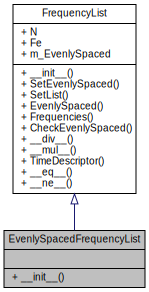
\includegraphics[width=221pt]{classSignalIntegrity_1_1FrequencyDomain_1_1FrequencyList_1_1EvenlySpacedFrequencyList__inherit__graph}
\end{center}
\end{figure}


Collaboration diagram for Evenly\+Spaced\+Frequency\+List\+:\nopagebreak
\begin{figure}[H]
\begin{center}
\leavevmode
\includegraphics[width=221pt]{classSignalIntegrity_1_1FrequencyDomain_1_1FrequencyList_1_1EvenlySpacedFrequencyList__coll__graph}
\end{center}
\end{figure}
\subsection*{Public Member Functions}
\begin{DoxyCompactItemize}
\item 
def \hyperlink{classSignalIntegrity_1_1FrequencyDomain_1_1FrequencyList_1_1EvenlySpacedFrequencyList_a14670857025f1633a7f1db215d83c385}{\+\_\+\+\_\+init\+\_\+\+\_\+} (self, \hyperlink{classSignalIntegrity_1_1FrequencyDomain_1_1FrequencyList_1_1FrequencyList_a7313483ea19e09cf50b8b58d531b871d}{Fe}, Np)
\begin{DoxyCompactList}\small\item\em Constructor. \end{DoxyCompactList}\end{DoxyCompactItemize}
\subsection*{Additional Inherited Members}


\subsection{Detailed Description}
A evenly spaced list of frequencies. 

Definition at line 196 of file Frequency\+List.\+py.



\subsection{Constructor \& Destructor Documentation}
\mbox{\Hypertarget{classSignalIntegrity_1_1FrequencyDomain_1_1FrequencyList_1_1EvenlySpacedFrequencyList_a14670857025f1633a7f1db215d83c385}\label{classSignalIntegrity_1_1FrequencyDomain_1_1FrequencyList_1_1EvenlySpacedFrequencyList_a14670857025f1633a7f1db215d83c385}} 
\index{Signal\+Integrity\+::\+Frequency\+Domain\+::\+Frequency\+List\+::\+Evenly\+Spaced\+Frequency\+List@{Signal\+Integrity\+::\+Frequency\+Domain\+::\+Frequency\+List\+::\+Evenly\+Spaced\+Frequency\+List}!\+\_\+\+\_\+init\+\_\+\+\_\+@{\+\_\+\+\_\+init\+\_\+\+\_\+}}
\index{\+\_\+\+\_\+init\+\_\+\+\_\+@{\+\_\+\+\_\+init\+\_\+\+\_\+}!Signal\+Integrity\+::\+Frequency\+Domain\+::\+Frequency\+List\+::\+Evenly\+Spaced\+Frequency\+List@{Signal\+Integrity\+::\+Frequency\+Domain\+::\+Frequency\+List\+::\+Evenly\+Spaced\+Frequency\+List}}
\subsubsection{\texorpdfstring{\+\_\+\+\_\+init\+\_\+\+\_\+()}{\_\_init\_\_()}}
{\footnotesize\ttfamily def \+\_\+\+\_\+init\+\_\+\+\_\+ (\begin{DoxyParamCaption}\item[{}]{self,  }\item[{}]{Fe,  }\item[{}]{Np }\end{DoxyParamCaption})}



Constructor. 


\begin{DoxyParams}{Parameters}
{\em Fe} & float end frequency for the frequency list. \\
\hline
{\em Np} & integer number of points (-\/1) or the frequency list (i.\+e. the number of points. in the new frequency list will be N+1. \\
\hline
\end{DoxyParams}
\begin{DoxyRemark}{Remarks}
Initializes the frequency list to be evenly spaced with Np+1 points from n=0..Np where each frequency is f\mbox{[}n\mbox{]}=n/\+Np$\ast$\+Fe. 
\end{DoxyRemark}


Definition at line 206 of file Frequency\+List.\+py.



The documentation for this class was generated from the following file\+:\begin{DoxyCompactItemize}
\item 
Py\+S\+I/\+Signal\+Integrity/\+Frequency\+Domain/Frequency\+List.\+py\end{DoxyCompactItemize}

\hypertarget{classSignalIntegrity_1_1TimeDomain_1_1Filters_1_1FilterDescriptor_1_1FilterDescriptor}{}\section{Filter\+Descriptor Class Reference}
\label{classSignalIntegrity_1_1TimeDomain_1_1Filters_1_1FilterDescriptor_1_1FilterDescriptor}\index{Filter\+Descriptor@{Filter\+Descriptor}}


handles time axis effects of filtering  




Inheritance diagram for Filter\+Descriptor\+:\nopagebreak
\begin{figure}[H]
\begin{center}
\leavevmode
\includegraphics[width=330pt]{classSignalIntegrity_1_1TimeDomain_1_1Filters_1_1FilterDescriptor_1_1FilterDescriptor__inherit__graph}
\end{center}
\end{figure}


Collaboration diagram for Filter\+Descriptor\+:\nopagebreak
\begin{figure}[H]
\begin{center}
\leavevmode
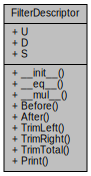
\includegraphics[width=163pt]{classSignalIntegrity_1_1TimeDomain_1_1Filters_1_1FilterDescriptor_1_1FilterDescriptor__coll__graph}
\end{center}
\end{figure}
\subsection*{Public Member Functions}
\begin{DoxyCompactItemize}
\item 
def \hyperlink{classSignalIntegrity_1_1TimeDomain_1_1Filters_1_1FilterDescriptor_1_1FilterDescriptor_a5661d52c9fb7ff469d450299f14df811}{\+\_\+\+\_\+init\+\_\+\+\_\+} (self, Upsample\+Factor, Delay\+Samples, Startup\+Samples)
\begin{DoxyCompactList}\small\item\em Constructor. \end{DoxyCompactList}\item 
def \hyperlink{classSignalIntegrity_1_1TimeDomain_1_1Filters_1_1FilterDescriptor_1_1FilterDescriptor_ad794ff077f2f05f228a7109f3670ac40}{\+\_\+\+\_\+eq\+\_\+\+\_\+} (self, other)
\begin{DoxyCompactList}\small\item\em overloads == \end{DoxyCompactList}\item 
def \hyperlink{classSignalIntegrity_1_1TimeDomain_1_1Filters_1_1FilterDescriptor_1_1FilterDescriptor_a96fd98a8997501189d60829abc0257cb}{\+\_\+\+\_\+mul\+\_\+\+\_\+} (self, other)
\begin{DoxyCompactList}\small\item\em overloads $\ast$~\newline
 multiplies two filter descriptors. \end{DoxyCompactList}\item 
def \hyperlink{classSignalIntegrity_1_1TimeDomain_1_1Filters_1_1FilterDescriptor_1_1FilterDescriptor_ae1c78203caa83b9eb7ecb92152f3488f}{Before} (self, other)
\begin{DoxyCompactList}\small\item\em calculates the effect of another filter before this one. \end{DoxyCompactList}\item 
def \hyperlink{classSignalIntegrity_1_1TimeDomain_1_1Filters_1_1FilterDescriptor_1_1FilterDescriptor_a29cf65c495a760f61e56af7b64342109}{After} (self, other)
\begin{DoxyCompactList}\small\item\em calculates the effect of another filter after this one. \end{DoxyCompactList}\item 
def \hyperlink{classSignalIntegrity_1_1TimeDomain_1_1Filters_1_1FilterDescriptor_1_1FilterDescriptor_aa755b1fade9a131f66c5a448181a158e}{Trim\+Left} (self)
\begin{DoxyCompactList}\small\item\em waveform points trimmed from the left \end{DoxyCompactList}\item 
def \hyperlink{classSignalIntegrity_1_1TimeDomain_1_1Filters_1_1FilterDescriptor_1_1FilterDescriptor_a284517d97da4a4e39890e41cbfa2a007}{Trim\+Right} (self)
\begin{DoxyCompactList}\small\item\em waveform points trimmed from the right \end{DoxyCompactList}\item 
def \hyperlink{classSignalIntegrity_1_1TimeDomain_1_1Filters_1_1FilterDescriptor_1_1FilterDescriptor_a8b3334081fe073524a4e0c068a61a3c6}{Trim\+Total} (self)
\begin{DoxyCompactList}\small\item\em waveform points trimmed in total \end{DoxyCompactList}\item 
\mbox{\Hypertarget{classSignalIntegrity_1_1TimeDomain_1_1Filters_1_1FilterDescriptor_1_1FilterDescriptor_a0203fc9c617eec80ba28741251ee3b86}\label{classSignalIntegrity_1_1TimeDomain_1_1Filters_1_1FilterDescriptor_1_1FilterDescriptor_a0203fc9c617eec80ba28741251ee3b86}} 
def \hyperlink{classSignalIntegrity_1_1TimeDomain_1_1Filters_1_1FilterDescriptor_1_1FilterDescriptor_a0203fc9c617eec80ba28741251ee3b86}{Print} (self)
\begin{DoxyCompactList}\small\item\em prints the filter descriptor in A\+S\+C\+II \end{DoxyCompactList}\end{DoxyCompactItemize}


\subsection{Detailed Description}
handles time axis effects of filtering 

Definition at line 12 of file Filter\+Descriptor.\+py.



\subsection{Constructor \& Destructor Documentation}
\mbox{\Hypertarget{classSignalIntegrity_1_1TimeDomain_1_1Filters_1_1FilterDescriptor_1_1FilterDescriptor_a5661d52c9fb7ff469d450299f14df811}\label{classSignalIntegrity_1_1TimeDomain_1_1Filters_1_1FilterDescriptor_1_1FilterDescriptor_a5661d52c9fb7ff469d450299f14df811}} 
\index{Signal\+Integrity\+::\+Time\+Domain\+::\+Filters\+::\+Filter\+Descriptor\+::\+Filter\+Descriptor@{Signal\+Integrity\+::\+Time\+Domain\+::\+Filters\+::\+Filter\+Descriptor\+::\+Filter\+Descriptor}!\+\_\+\+\_\+init\+\_\+\+\_\+@{\+\_\+\+\_\+init\+\_\+\+\_\+}}
\index{\+\_\+\+\_\+init\+\_\+\+\_\+@{\+\_\+\+\_\+init\+\_\+\+\_\+}!Signal\+Integrity\+::\+Time\+Domain\+::\+Filters\+::\+Filter\+Descriptor\+::\+Filter\+Descriptor@{Signal\+Integrity\+::\+Time\+Domain\+::\+Filters\+::\+Filter\+Descriptor\+::\+Filter\+Descriptor}}
\subsubsection{\texorpdfstring{\+\_\+\+\_\+init\+\_\+\+\_\+()}{\_\_init\_\_()}}
{\footnotesize\ttfamily def \+\_\+\+\_\+init\+\_\+\+\_\+ (\begin{DoxyParamCaption}\item[{}]{self,  }\item[{}]{Upsample\+Factor,  }\item[{}]{Delay\+Samples,  }\item[{}]{Startup\+Samples }\end{DoxyParamCaption})}



Constructor. 


\begin{DoxyParams}{Parameters}
{\em Upsample\+Factor} & integer or float upsample factor. This is the multiplicative factor that the filter will have on the sample rate of an applied waveform. \\
\hline
{\em Delay\+Samples} & integer or float samples that the filter applies to a waveform. \\
\hline
{\em Startup\+Samples} & integer or float the number of samples that must be removed from the filtered waveform due to filter startup effects. \\
\hline
\end{DoxyParams}


Definition at line 21 of file Filter\+Descriptor.\+py.



\subsection{Member Function Documentation}
\mbox{\Hypertarget{classSignalIntegrity_1_1TimeDomain_1_1Filters_1_1FilterDescriptor_1_1FilterDescriptor_ad794ff077f2f05f228a7109f3670ac40}\label{classSignalIntegrity_1_1TimeDomain_1_1Filters_1_1FilterDescriptor_1_1FilterDescriptor_ad794ff077f2f05f228a7109f3670ac40}} 
\index{Signal\+Integrity\+::\+Time\+Domain\+::\+Filters\+::\+Filter\+Descriptor\+::\+Filter\+Descriptor@{Signal\+Integrity\+::\+Time\+Domain\+::\+Filters\+::\+Filter\+Descriptor\+::\+Filter\+Descriptor}!\+\_\+\+\_\+eq\+\_\+\+\_\+@{\+\_\+\+\_\+eq\+\_\+\+\_\+}}
\index{\+\_\+\+\_\+eq\+\_\+\+\_\+@{\+\_\+\+\_\+eq\+\_\+\+\_\+}!Signal\+Integrity\+::\+Time\+Domain\+::\+Filters\+::\+Filter\+Descriptor\+::\+Filter\+Descriptor@{Signal\+Integrity\+::\+Time\+Domain\+::\+Filters\+::\+Filter\+Descriptor\+::\+Filter\+Descriptor}}
\subsubsection{\texorpdfstring{\+\_\+\+\_\+eq\+\_\+\+\_\+()}{\_\_eq\_\_()}}
{\footnotesize\ttfamily def \+\_\+\+\_\+eq\+\_\+\+\_\+ (\begin{DoxyParamCaption}\item[{}]{self,  }\item[{}]{other }\end{DoxyParamCaption})}



overloads == 

\begin{DoxyReturn}{Returns}
boolean whether to filter descriptors are the same 
\end{DoxyReturn}


Definition at line 29 of file Filter\+Descriptor.\+py.

\mbox{\Hypertarget{classSignalIntegrity_1_1TimeDomain_1_1Filters_1_1FilterDescriptor_1_1FilterDescriptor_a96fd98a8997501189d60829abc0257cb}\label{classSignalIntegrity_1_1TimeDomain_1_1Filters_1_1FilterDescriptor_1_1FilterDescriptor_a96fd98a8997501189d60829abc0257cb}} 
\index{Signal\+Integrity\+::\+Time\+Domain\+::\+Filters\+::\+Filter\+Descriptor\+::\+Filter\+Descriptor@{Signal\+Integrity\+::\+Time\+Domain\+::\+Filters\+::\+Filter\+Descriptor\+::\+Filter\+Descriptor}!\+\_\+\+\_\+mul\+\_\+\+\_\+@{\+\_\+\+\_\+mul\+\_\+\+\_\+}}
\index{\+\_\+\+\_\+mul\+\_\+\+\_\+@{\+\_\+\+\_\+mul\+\_\+\+\_\+}!Signal\+Integrity\+::\+Time\+Domain\+::\+Filters\+::\+Filter\+Descriptor\+::\+Filter\+Descriptor@{Signal\+Integrity\+::\+Time\+Domain\+::\+Filters\+::\+Filter\+Descriptor\+::\+Filter\+Descriptor}}
\subsubsection{\texorpdfstring{\+\_\+\+\_\+mul\+\_\+\+\_\+()}{\_\_mul\_\_()}}
{\footnotesize\ttfamily def \+\_\+\+\_\+mul\+\_\+\+\_\+ (\begin{DoxyParamCaption}\item[{}]{self,  }\item[{}]{other }\end{DoxyParamCaption})}



overloads $\ast$~\newline
 multiplies two filter descriptors. 

This is the same as calculating the effect of the two filters in cascade. 
\begin{DoxyParams}{Parameters}
{\em other} & an instance of class \hyperlink{classSignalIntegrity_1_1TimeDomain_1_1Filters_1_1FilterDescriptor_1_1FilterDescriptor}{Filter\+Descriptor} of another filter \\
\hline
\end{DoxyParams}
\begin{DoxyReturn}{Returns}
instance of class \hyperlink{classSignalIntegrity_1_1TimeDomain_1_1Filters_1_1FilterDescriptor_1_1FilterDescriptor}{Filter\+Descriptor} of the cascaded filters 
\end{DoxyReturn}


Definition at line 41 of file Filter\+Descriptor.\+py.

\mbox{\Hypertarget{classSignalIntegrity_1_1TimeDomain_1_1Filters_1_1FilterDescriptor_1_1FilterDescriptor_a29cf65c495a760f61e56af7b64342109}\label{classSignalIntegrity_1_1TimeDomain_1_1Filters_1_1FilterDescriptor_1_1FilterDescriptor_a29cf65c495a760f61e56af7b64342109}} 
\index{Signal\+Integrity\+::\+Time\+Domain\+::\+Filters\+::\+Filter\+Descriptor\+::\+Filter\+Descriptor@{Signal\+Integrity\+::\+Time\+Domain\+::\+Filters\+::\+Filter\+Descriptor\+::\+Filter\+Descriptor}!After@{After}}
\index{After@{After}!Signal\+Integrity\+::\+Time\+Domain\+::\+Filters\+::\+Filter\+Descriptor\+::\+Filter\+Descriptor@{Signal\+Integrity\+::\+Time\+Domain\+::\+Filters\+::\+Filter\+Descriptor\+::\+Filter\+Descriptor}}
\subsubsection{\texorpdfstring{After()}{After()}}
{\footnotesize\ttfamily def After (\begin{DoxyParamCaption}\item[{}]{self,  }\item[{}]{other }\end{DoxyParamCaption})}



calculates the effect of another filter after this one. 


\begin{DoxyParams}{Parameters}
{\em other} & an instance of class \hyperlink{classSignalIntegrity_1_1TimeDomain_1_1Filters_1_1FilterDescriptor_1_1FilterDescriptor}{Filter\+Descriptor} of another filter \\
\hline
\end{DoxyParams}
\begin{DoxyReturn}{Returns}
instance of class \hyperlink{classSignalIntegrity_1_1TimeDomain_1_1Filters_1_1FilterDescriptor_1_1FilterDescriptor}{Filter\+Descriptor} of the other filter moved after this one 
\end{DoxyReturn}


Definition at line 62 of file Filter\+Descriptor.\+py.

\mbox{\Hypertarget{classSignalIntegrity_1_1TimeDomain_1_1Filters_1_1FilterDescriptor_1_1FilterDescriptor_ae1c78203caa83b9eb7ecb92152f3488f}\label{classSignalIntegrity_1_1TimeDomain_1_1Filters_1_1FilterDescriptor_1_1FilterDescriptor_ae1c78203caa83b9eb7ecb92152f3488f}} 
\index{Signal\+Integrity\+::\+Time\+Domain\+::\+Filters\+::\+Filter\+Descriptor\+::\+Filter\+Descriptor@{Signal\+Integrity\+::\+Time\+Domain\+::\+Filters\+::\+Filter\+Descriptor\+::\+Filter\+Descriptor}!Before@{Before}}
\index{Before@{Before}!Signal\+Integrity\+::\+Time\+Domain\+::\+Filters\+::\+Filter\+Descriptor\+::\+Filter\+Descriptor@{Signal\+Integrity\+::\+Time\+Domain\+::\+Filters\+::\+Filter\+Descriptor\+::\+Filter\+Descriptor}}
\subsubsection{\texorpdfstring{Before()}{Before()}}
{\footnotesize\ttfamily def Before (\begin{DoxyParamCaption}\item[{}]{self,  }\item[{}]{other }\end{DoxyParamCaption})}



calculates the effect of another filter before this one. 


\begin{DoxyParams}{Parameters}
{\em other} & an instance of class \hyperlink{classSignalIntegrity_1_1TimeDomain_1_1Filters_1_1FilterDescriptor_1_1FilterDescriptor}{Filter\+Descriptor} of another filter \\
\hline
\end{DoxyParams}
\begin{DoxyReturn}{Returns}
instance of class \hyperlink{classSignalIntegrity_1_1TimeDomain_1_1Filters_1_1FilterDescriptor_1_1FilterDescriptor}{Filter\+Descriptor} of the other filter moved before this one 
\end{DoxyReturn}


Definition at line 52 of file Filter\+Descriptor.\+py.

\mbox{\Hypertarget{classSignalIntegrity_1_1TimeDomain_1_1Filters_1_1FilterDescriptor_1_1FilterDescriptor_aa755b1fade9a131f66c5a448181a158e}\label{classSignalIntegrity_1_1TimeDomain_1_1Filters_1_1FilterDescriptor_1_1FilterDescriptor_aa755b1fade9a131f66c5a448181a158e}} 
\index{Signal\+Integrity\+::\+Time\+Domain\+::\+Filters\+::\+Filter\+Descriptor\+::\+Filter\+Descriptor@{Signal\+Integrity\+::\+Time\+Domain\+::\+Filters\+::\+Filter\+Descriptor\+::\+Filter\+Descriptor}!Trim\+Left@{Trim\+Left}}
\index{Trim\+Left@{Trim\+Left}!Signal\+Integrity\+::\+Time\+Domain\+::\+Filters\+::\+Filter\+Descriptor\+::\+Filter\+Descriptor@{Signal\+Integrity\+::\+Time\+Domain\+::\+Filters\+::\+Filter\+Descriptor\+::\+Filter\+Descriptor}}
\subsubsection{\texorpdfstring{Trim\+Left()}{TrimLeft()}}
{\footnotesize\ttfamily def Trim\+Left (\begin{DoxyParamCaption}\item[{}]{self }\end{DoxyParamCaption})}



waveform points trimmed from the left 

\begin{DoxyReturn}{Returns}
the number of waveform points trimmed from the left by applying this filter 
\end{DoxyReturn}


Definition at line 71 of file Filter\+Descriptor.\+py.

\mbox{\Hypertarget{classSignalIntegrity_1_1TimeDomain_1_1Filters_1_1FilterDescriptor_1_1FilterDescriptor_a284517d97da4a4e39890e41cbfa2a007}\label{classSignalIntegrity_1_1TimeDomain_1_1Filters_1_1FilterDescriptor_1_1FilterDescriptor_a284517d97da4a4e39890e41cbfa2a007}} 
\index{Signal\+Integrity\+::\+Time\+Domain\+::\+Filters\+::\+Filter\+Descriptor\+::\+Filter\+Descriptor@{Signal\+Integrity\+::\+Time\+Domain\+::\+Filters\+::\+Filter\+Descriptor\+::\+Filter\+Descriptor}!Trim\+Right@{Trim\+Right}}
\index{Trim\+Right@{Trim\+Right}!Signal\+Integrity\+::\+Time\+Domain\+::\+Filters\+::\+Filter\+Descriptor\+::\+Filter\+Descriptor@{Signal\+Integrity\+::\+Time\+Domain\+::\+Filters\+::\+Filter\+Descriptor\+::\+Filter\+Descriptor}}
\subsubsection{\texorpdfstring{Trim\+Right()}{TrimRight()}}
{\footnotesize\ttfamily def Trim\+Right (\begin{DoxyParamCaption}\item[{}]{self }\end{DoxyParamCaption})}



waveform points trimmed from the right 

\begin{DoxyReturn}{Returns}
the number of waveform points trimmed from the right by applying this filter 
\end{DoxyReturn}


Definition at line 77 of file Filter\+Descriptor.\+py.

\mbox{\Hypertarget{classSignalIntegrity_1_1TimeDomain_1_1Filters_1_1FilterDescriptor_1_1FilterDescriptor_a8b3334081fe073524a4e0c068a61a3c6}\label{classSignalIntegrity_1_1TimeDomain_1_1Filters_1_1FilterDescriptor_1_1FilterDescriptor_a8b3334081fe073524a4e0c068a61a3c6}} 
\index{Signal\+Integrity\+::\+Time\+Domain\+::\+Filters\+::\+Filter\+Descriptor\+::\+Filter\+Descriptor@{Signal\+Integrity\+::\+Time\+Domain\+::\+Filters\+::\+Filter\+Descriptor\+::\+Filter\+Descriptor}!Trim\+Total@{Trim\+Total}}
\index{Trim\+Total@{Trim\+Total}!Signal\+Integrity\+::\+Time\+Domain\+::\+Filters\+::\+Filter\+Descriptor\+::\+Filter\+Descriptor@{Signal\+Integrity\+::\+Time\+Domain\+::\+Filters\+::\+Filter\+Descriptor\+::\+Filter\+Descriptor}}
\subsubsection{\texorpdfstring{Trim\+Total()}{TrimTotal()}}
{\footnotesize\ttfamily def Trim\+Total (\begin{DoxyParamCaption}\item[{}]{self }\end{DoxyParamCaption})}



waveform points trimmed in total 

\begin{DoxyReturn}{Returns}
the total number of waveform points trimmed by applying this filter 
\end{DoxyReturn}


Definition at line 83 of file Filter\+Descriptor.\+py.



The documentation for this class was generated from the following file\+:\begin{DoxyCompactItemize}
\item 
Py\+S\+I/\+Signal\+Integrity/\+Time\+Domain/\+Filters/Filter\+Descriptor.\+py\end{DoxyCompactItemize}

\hypertarget{classSignalIntegrity_1_1TimeDomain_1_1Filters_1_1FirFilter_1_1FirFilter}{}\section{Fir\+Filter Class Reference}
\label{classSignalIntegrity_1_1TimeDomain_1_1Filters_1_1FirFilter_1_1FirFilter}\index{Fir\+Filter@{Fir\+Filter}}


base filter class for all F\+IR filters  




Inheritance diagram for Fir\+Filter\+:
\nopagebreak
\begin{figure}[H]
\begin{center}
\leavevmode
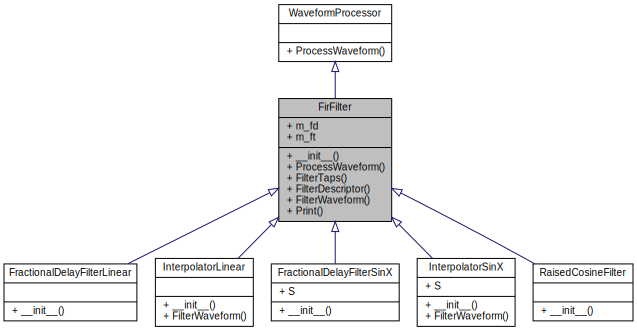
\includegraphics[width=350pt]{classSignalIntegrity_1_1TimeDomain_1_1Filters_1_1FirFilter_1_1FirFilter__inherit__graph}
\end{center}
\end{figure}


Collaboration diagram for Fir\+Filter\+:
\nopagebreak
\begin{figure}[H]
\begin{center}
\leavevmode
\includegraphics[width=193pt]{classSignalIntegrity_1_1TimeDomain_1_1Filters_1_1FirFilter_1_1FirFilter__coll__graph}
\end{center}
\end{figure}
\subsection*{Public Member Functions}
\begin{DoxyCompactItemize}
\item 
def \hyperlink{classSignalIntegrity_1_1TimeDomain_1_1Filters_1_1FirFilter_1_1FirFilter_aa769a401c278ca11fba676e33af50456}{\+\_\+\+\_\+init\+\_\+\+\_\+} (self, fd, ft)
\begin{DoxyCompactList}\small\item\em Constructor. \end{DoxyCompactList}\item 
def \hyperlink{classSignalIntegrity_1_1TimeDomain_1_1Filters_1_1FirFilter_1_1FirFilter_ae09bec195c9cb1d5819e73b7be169b11}{Process\+Waveform} (self, wf)
\begin{DoxyCompactList}\small\item\em process waveform \end{DoxyCompactList}\item 
def \hyperlink{classSignalIntegrity_1_1TimeDomain_1_1Filters_1_1FirFilter_1_1FirFilter_a215bb8b37eed7c3d66ece034a41dcb75}{Filter\+Taps} (self)
\begin{DoxyCompactList}\small\item\em return the filter taps \end{DoxyCompactList}\item 
def \hyperlink{classSignalIntegrity_1_1TimeDomain_1_1Filters_1_1FirFilter_1_1FirFilter_a68fed1ece509bfbd2f3ae97633d5579d}{Filter\+Descriptor} (self)
\begin{DoxyCompactList}\small\item\em returns the filter descriptor \end{DoxyCompactList}\item 
def \hyperlink{classSignalIntegrity_1_1TimeDomain_1_1Filters_1_1FirFilter_1_1FirFilter_a84e73c18250ca4a61482f94ad61e735b}{Filter\+Waveform} (self, wf)
\begin{DoxyCompactList}\small\item\em filters a waveform \end{DoxyCompactList}\item 
\mbox{\Hypertarget{classSignalIntegrity_1_1TimeDomain_1_1Filters_1_1FirFilter_1_1FirFilter_a0203fc9c617eec80ba28741251ee3b86}\label{classSignalIntegrity_1_1TimeDomain_1_1Filters_1_1FirFilter_1_1FirFilter_a0203fc9c617eec80ba28741251ee3b86}} 
def \hyperlink{classSignalIntegrity_1_1TimeDomain_1_1Filters_1_1FirFilter_1_1FirFilter_a0203fc9c617eec80ba28741251ee3b86}{Print} (self)
\begin{DoxyCompactList}\small\item\em prints an A\+S\+C\+II description of the filter \end{DoxyCompactList}\end{DoxyCompactItemize}


\subsection{Detailed Description}
base filter class for all F\+IR filters 

Definition at line 24 of file Fir\+Filter.\+py.



\subsection{Constructor \& Destructor Documentation}
\mbox{\Hypertarget{classSignalIntegrity_1_1TimeDomain_1_1Filters_1_1FirFilter_1_1FirFilter_aa769a401c278ca11fba676e33af50456}\label{classSignalIntegrity_1_1TimeDomain_1_1Filters_1_1FirFilter_1_1FirFilter_aa769a401c278ca11fba676e33af50456}} 
\index{Signal\+Integrity\+::\+Time\+Domain\+::\+Filters\+::\+Fir\+Filter\+::\+Fir\+Filter@{Signal\+Integrity\+::\+Time\+Domain\+::\+Filters\+::\+Fir\+Filter\+::\+Fir\+Filter}!\+\_\+\+\_\+init\+\_\+\+\_\+@{\+\_\+\+\_\+init\+\_\+\+\_\+}}
\index{\+\_\+\+\_\+init\+\_\+\+\_\+@{\+\_\+\+\_\+init\+\_\+\+\_\+}!Signal\+Integrity\+::\+Time\+Domain\+::\+Filters\+::\+Fir\+Filter\+::\+Fir\+Filter@{Signal\+Integrity\+::\+Time\+Domain\+::\+Filters\+::\+Fir\+Filter\+::\+Fir\+Filter}}
\subsubsection{\texorpdfstring{\+\_\+\+\_\+init\+\_\+\+\_\+()}{\_\_init\_\_()}}
{\footnotesize\ttfamily def \+\_\+\+\_\+init\+\_\+\+\_\+ (\begin{DoxyParamCaption}\item[{}]{self,  }\item[{}]{fd,  }\item[{}]{ft }\end{DoxyParamCaption})}



Constructor. 


\begin{DoxyParams}{Parameters}
{\em fd} & instance of class \hyperlink{namespaceSignalIntegrity_1_1TimeDomain_1_1Filters_1_1FilterDescriptor}{Filter\+Descriptor} describing the time axis effects of this filter. \\
\hline
{\em ft} & list of float filter taps \\
\hline
\end{DoxyParams}


Definition at line 31 of file Fir\+Filter.\+py.



\subsection{Member Function Documentation}
\mbox{\Hypertarget{classSignalIntegrity_1_1TimeDomain_1_1Filters_1_1FirFilter_1_1FirFilter_a68fed1ece509bfbd2f3ae97633d5579d}\label{classSignalIntegrity_1_1TimeDomain_1_1Filters_1_1FirFilter_1_1FirFilter_a68fed1ece509bfbd2f3ae97633d5579d}} 
\index{Signal\+Integrity\+::\+Time\+Domain\+::\+Filters\+::\+Fir\+Filter\+::\+Fir\+Filter@{Signal\+Integrity\+::\+Time\+Domain\+::\+Filters\+::\+Fir\+Filter\+::\+Fir\+Filter}!Filter\+Descriptor@{Filter\+Descriptor}}
\index{Filter\+Descriptor@{Filter\+Descriptor}!Signal\+Integrity\+::\+Time\+Domain\+::\+Filters\+::\+Fir\+Filter\+::\+Fir\+Filter@{Signal\+Integrity\+::\+Time\+Domain\+::\+Filters\+::\+Fir\+Filter\+::\+Fir\+Filter}}
\subsubsection{\texorpdfstring{Filter\+Descriptor()}{FilterDescriptor()}}
{\footnotesize\ttfamily def \hyperlink{classSignalIntegrity_1_1TimeDomain_1_1Filters_1_1FilterDescriptor_1_1FilterDescriptor}{Filter\+Descriptor} (\begin{DoxyParamCaption}\item[{}]{self }\end{DoxyParamCaption})}



returns the filter descriptor 

\begin{DoxyReturn}{Returns}
instance of class \hyperlink{namespaceSignalIntegrity_1_1TimeDomain_1_1Filters_1_1FilterDescriptor}{Filter\+Descriptor} 
\end{DoxyReturn}


Definition at line 55 of file Fir\+Filter.\+py.

\mbox{\Hypertarget{classSignalIntegrity_1_1TimeDomain_1_1Filters_1_1FirFilter_1_1FirFilter_a215bb8b37eed7c3d66ece034a41dcb75}\label{classSignalIntegrity_1_1TimeDomain_1_1Filters_1_1FirFilter_1_1FirFilter_a215bb8b37eed7c3d66ece034a41dcb75}} 
\index{Signal\+Integrity\+::\+Time\+Domain\+::\+Filters\+::\+Fir\+Filter\+::\+Fir\+Filter@{Signal\+Integrity\+::\+Time\+Domain\+::\+Filters\+::\+Fir\+Filter\+::\+Fir\+Filter}!Filter\+Taps@{Filter\+Taps}}
\index{Filter\+Taps@{Filter\+Taps}!Signal\+Integrity\+::\+Time\+Domain\+::\+Filters\+::\+Fir\+Filter\+::\+Fir\+Filter@{Signal\+Integrity\+::\+Time\+Domain\+::\+Filters\+::\+Fir\+Filter\+::\+Fir\+Filter}}
\subsubsection{\texorpdfstring{Filter\+Taps()}{FilterTaps()}}
{\footnotesize\ttfamily def Filter\+Taps (\begin{DoxyParamCaption}\item[{}]{self }\end{DoxyParamCaption})}



return the filter taps 

\begin{DoxyReturn}{Returns}
list of float filter taps 
\end{DoxyReturn}


Definition at line 49 of file Fir\+Filter.\+py.

\mbox{\Hypertarget{classSignalIntegrity_1_1TimeDomain_1_1Filters_1_1FirFilter_1_1FirFilter_a84e73c18250ca4a61482f94ad61e735b}\label{classSignalIntegrity_1_1TimeDomain_1_1Filters_1_1FirFilter_1_1FirFilter_a84e73c18250ca4a61482f94ad61e735b}} 
\index{Signal\+Integrity\+::\+Time\+Domain\+::\+Filters\+::\+Fir\+Filter\+::\+Fir\+Filter@{Signal\+Integrity\+::\+Time\+Domain\+::\+Filters\+::\+Fir\+Filter\+::\+Fir\+Filter}!Filter\+Waveform@{Filter\+Waveform}}
\index{Filter\+Waveform@{Filter\+Waveform}!Signal\+Integrity\+::\+Time\+Domain\+::\+Filters\+::\+Fir\+Filter\+::\+Fir\+Filter@{Signal\+Integrity\+::\+Time\+Domain\+::\+Filters\+::\+Fir\+Filter\+::\+Fir\+Filter}}
\subsubsection{\texorpdfstring{Filter\+Waveform()}{FilterWaveform()}}
{\footnotesize\ttfamily def Filter\+Waveform (\begin{DoxyParamCaption}\item[{}]{self,  }\item[{}]{wf }\end{DoxyParamCaption})}



filters a waveform 


\begin{DoxyParams}{Parameters}
{\em wf} & instance of class \hyperlink{namespaceSignalIntegrity_1_1TimeDomain_1_1Waveform}{Waveform} \\
\hline
\end{DoxyParams}
\begin{DoxyReturn}{Returns}
instance of class \hyperlink{namespaceSignalIntegrity_1_1TimeDomain_1_1Waveform}{Waveform} containing this filter applied to wf 
\end{DoxyReturn}


Definition at line 62 of file Fir\+Filter.\+py.

\mbox{\Hypertarget{classSignalIntegrity_1_1TimeDomain_1_1Filters_1_1FirFilter_1_1FirFilter_ae09bec195c9cb1d5819e73b7be169b11}\label{classSignalIntegrity_1_1TimeDomain_1_1Filters_1_1FirFilter_1_1FirFilter_ae09bec195c9cb1d5819e73b7be169b11}} 
\index{Signal\+Integrity\+::\+Time\+Domain\+::\+Filters\+::\+Fir\+Filter\+::\+Fir\+Filter@{Signal\+Integrity\+::\+Time\+Domain\+::\+Filters\+::\+Fir\+Filter\+::\+Fir\+Filter}!Process\+Waveform@{Process\+Waveform}}
\index{Process\+Waveform@{Process\+Waveform}!Signal\+Integrity\+::\+Time\+Domain\+::\+Filters\+::\+Fir\+Filter\+::\+Fir\+Filter@{Signal\+Integrity\+::\+Time\+Domain\+::\+Filters\+::\+Fir\+Filter\+::\+Fir\+Filter}}
\subsubsection{\texorpdfstring{Process\+Waveform()}{ProcessWaveform()}}
{\footnotesize\ttfamily def Process\+Waveform (\begin{DoxyParamCaption}\item[{}]{self,  }\item[{}]{wf }\end{DoxyParamCaption})}



process waveform 

F\+IR filters process waveforms by filtering them.


\begin{DoxyParams}{Parameters}
{\em wf} & instance of class \hyperlink{namespaceSignalIntegrity_1_1TimeDomain_1_1Waveform}{Waveform} to filter \\
\hline
\end{DoxyParams}
\begin{DoxyReturn}{Returns}
instance of class \hyperlink{namespaceSignalIntegrity_1_1TimeDomain_1_1Waveform}{Waveform} containing this filter applied to wf 
\end{DoxyReturn}
\begin{DoxySeeAlso}{See also}
\hyperlink{classSignalIntegrity_1_1TimeDomain_1_1Filters_1_1FirFilter_1_1FirFilter_a84e73c18250ca4a61482f94ad61e735b}{Filter\+Waveform} 
\end{DoxySeeAlso}


Definition at line 43 of file Fir\+Filter.\+py.



The documentation for this class was generated from the following file\+:\begin{DoxyCompactItemize}
\item 
Py\+S\+I/\+Signal\+Integrity/\+Time\+Domain/\+Filters/Fir\+Filter.\+py\end{DoxyCompactItemize}

\hypertarget{classSignalIntegrity_1_1TimeDomain_1_1Filters_1_1InterpolatorLinear_1_1FractionalDelayFilterLinear}{}\section{Fractional\+Delay\+Filter\+Linear Class Reference}
\label{classSignalIntegrity_1_1TimeDomain_1_1Filters_1_1InterpolatorLinear_1_1FractionalDelayFilterLinear}\index{Fractional\+Delay\+Filter\+Linear@{Fractional\+Delay\+Filter\+Linear}}


linear fractional delay filter  




Inheritance diagram for Fractional\+Delay\+Filter\+Linear\+:
\nopagebreak
\begin{figure}[H]
\begin{center}
\leavevmode
\includegraphics[width=213pt]{classSignalIntegrity_1_1TimeDomain_1_1Filters_1_1InterpolatorLinear_1_1FractionalDelayFilterLinear__inherit__graph}
\end{center}
\end{figure}


Collaboration diagram for Fractional\+Delay\+Filter\+Linear\+:
\nopagebreak
\begin{figure}[H]
\begin{center}
\leavevmode
\includegraphics[width=213pt]{classSignalIntegrity_1_1TimeDomain_1_1Filters_1_1InterpolatorLinear_1_1FractionalDelayFilterLinear__coll__graph}
\end{center}
\end{figure}
\subsection*{Public Member Functions}
\begin{DoxyCompactItemize}
\item 
def \hyperlink{classSignalIntegrity_1_1TimeDomain_1_1Filters_1_1InterpolatorLinear_1_1FractionalDelayFilterLinear_a71162faa904c7ea2018b89ebba16c33d}{\+\_\+\+\_\+init\+\_\+\+\_\+} (self, F, account\+For\+Delay=True)
\begin{DoxyCompactList}\small\item\em Constructor. \end{DoxyCompactList}\end{DoxyCompactItemize}


\subsection{Detailed Description}
linear fractional delay filter 

Definition at line 22 of file Interpolator\+Linear.\+py.



\subsection{Constructor \& Destructor Documentation}
\mbox{\Hypertarget{classSignalIntegrity_1_1TimeDomain_1_1Filters_1_1InterpolatorLinear_1_1FractionalDelayFilterLinear_a71162faa904c7ea2018b89ebba16c33d}\label{classSignalIntegrity_1_1TimeDomain_1_1Filters_1_1InterpolatorLinear_1_1FractionalDelayFilterLinear_a71162faa904c7ea2018b89ebba16c33d}} 
\index{Signal\+Integrity\+::\+Time\+Domain\+::\+Filters\+::\+Interpolator\+Linear\+::\+Fractional\+Delay\+Filter\+Linear@{Signal\+Integrity\+::\+Time\+Domain\+::\+Filters\+::\+Interpolator\+Linear\+::\+Fractional\+Delay\+Filter\+Linear}!\+\_\+\+\_\+init\+\_\+\+\_\+@{\+\_\+\+\_\+init\+\_\+\+\_\+}}
\index{\+\_\+\+\_\+init\+\_\+\+\_\+@{\+\_\+\+\_\+init\+\_\+\+\_\+}!Signal\+Integrity\+::\+Time\+Domain\+::\+Filters\+::\+Interpolator\+Linear\+::\+Fractional\+Delay\+Filter\+Linear@{Signal\+Integrity\+::\+Time\+Domain\+::\+Filters\+::\+Interpolator\+Linear\+::\+Fractional\+Delay\+Filter\+Linear}}
\subsubsection{\texorpdfstring{\+\_\+\+\_\+init\+\_\+\+\_\+()}{\_\_init\_\_()}}
{\footnotesize\ttfamily def \+\_\+\+\_\+init\+\_\+\+\_\+ (\begin{DoxyParamCaption}\item[{}]{self,  }\item[{}]{F,  }\item[{}]{account\+For\+Delay = {\ttfamily True} }\end{DoxyParamCaption})}



Constructor. 

applies a two-\/tap linear interpolating filter.


\begin{DoxyParams}{Parameters}
{\em F} & float amount of delay to apply. The delay is in samples of the input waveform. \\
\hline
{\em account\+For\+Delay} & (optional) boolean whether to account for the delay \\
\hline
\end{DoxyParams}
\begin{DoxyRemark}{Remarks}
if account\+For\+Delay, then the filter provides a sample phase adjustment, meaning that there is no actual delay applied to the waveform, but the time axis under the waveform is shifted. This is the usual way to apply this filter and is used to adapt waveforms on different time axes to each other.~\newline
 if not account\+For\+Delay, then the filter actually delays waveforms by the delay specified. 
\end{DoxyRemark}


Definition at line 38 of file Interpolator\+Linear.\+py.



The documentation for this class was generated from the following file\+:\begin{DoxyCompactItemize}
\item 
Py\+S\+I/\+Signal\+Integrity/\+Time\+Domain/\+Filters/Interpolator\+Linear.\+py\end{DoxyCompactItemize}

\hypertarget{classSignalIntegrity_1_1TimeDomain_1_1Filters_1_1InterpolatorSinX_1_1FractionalDelayFilterSinX}{}\section{Fractional\+Delay\+Filter\+SinX Class Reference}
\label{classSignalIntegrity_1_1TimeDomain_1_1Filters_1_1InterpolatorSinX_1_1FractionalDelayFilterSinX}\index{Fractional\+Delay\+Filter\+SinX@{Fractional\+Delay\+Filter\+SinX}}


sinx/x fractional delay filter  




Inheritance diagram for Fractional\+Delay\+Filter\+SinX\+:\nopagebreak
\begin{figure}[H]
\begin{center}
\leavevmode
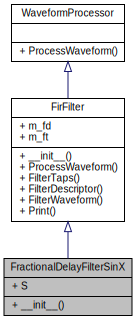
\includegraphics[width=208pt]{classSignalIntegrity_1_1TimeDomain_1_1Filters_1_1InterpolatorSinX_1_1FractionalDelayFilterSinX__inherit__graph}
\end{center}
\end{figure}


Collaboration diagram for Fractional\+Delay\+Filter\+SinX\+:\nopagebreak
\begin{figure}[H]
\begin{center}
\leavevmode
\includegraphics[width=208pt]{classSignalIntegrity_1_1TimeDomain_1_1Filters_1_1InterpolatorSinX_1_1FractionalDelayFilterSinX__coll__graph}
\end{center}
\end{figure}
\subsection*{Public Member Functions}
\begin{DoxyCompactItemize}
\item 
def \hyperlink{classSignalIntegrity_1_1TimeDomain_1_1Filters_1_1InterpolatorSinX_1_1FractionalDelayFilterSinX_a71162faa904c7ea2018b89ebba16c33d}{\+\_\+\+\_\+init\+\_\+\+\_\+} (self, F, account\+For\+Delay=True)
\begin{DoxyCompactList}\small\item\em Constructor. \end{DoxyCompactList}\end{DoxyCompactItemize}


\subsection{Detailed Description}
sinx/x fractional delay filter 

Definition at line 37 of file Interpolator\+Sin\+X.\+py.



\subsection{Constructor \& Destructor Documentation}
\mbox{\Hypertarget{classSignalIntegrity_1_1TimeDomain_1_1Filters_1_1InterpolatorSinX_1_1FractionalDelayFilterSinX_a71162faa904c7ea2018b89ebba16c33d}\label{classSignalIntegrity_1_1TimeDomain_1_1Filters_1_1InterpolatorSinX_1_1FractionalDelayFilterSinX_a71162faa904c7ea2018b89ebba16c33d}} 
\index{Signal\+Integrity\+::\+Time\+Domain\+::\+Filters\+::\+Interpolator\+Sin\+X\+::\+Fractional\+Delay\+Filter\+SinX@{Signal\+Integrity\+::\+Time\+Domain\+::\+Filters\+::\+Interpolator\+Sin\+X\+::\+Fractional\+Delay\+Filter\+SinX}!\+\_\+\+\_\+init\+\_\+\+\_\+@{\+\_\+\+\_\+init\+\_\+\+\_\+}}
\index{\+\_\+\+\_\+init\+\_\+\+\_\+@{\+\_\+\+\_\+init\+\_\+\+\_\+}!Signal\+Integrity\+::\+Time\+Domain\+::\+Filters\+::\+Interpolator\+Sin\+X\+::\+Fractional\+Delay\+Filter\+SinX@{Signal\+Integrity\+::\+Time\+Domain\+::\+Filters\+::\+Interpolator\+Sin\+X\+::\+Fractional\+Delay\+Filter\+SinX}}
\subsubsection{\texorpdfstring{\+\_\+\+\_\+init\+\_\+\+\_\+()}{\_\_init\_\_()}}
{\footnotesize\ttfamily def \+\_\+\+\_\+init\+\_\+\+\_\+ (\begin{DoxyParamCaption}\item[{}]{self,  }\item[{}]{F,  }\item[{}]{account\+For\+Delay = {\ttfamily True} }\end{DoxyParamCaption})}



Constructor. 

applies sinx/x interpolating filter.


\begin{DoxyParams}{Parameters}
{\em F} & float amount of delay to apply. The delay is in samples of the input waveform. \\
\hline
{\em account\+For\+Delay} & (optional) boolean whether to account for the delay \\
\hline
\end{DoxyParams}
\begin{DoxyRemark}{Remarks}
if account\+For\+Delay, then the filter provides a sample phase adjustment, meaning that there is no actual delay applied to the waveform, but the time axis under the waveform is shifted. This is the usual way to apply this filter and is used to adapt waveforms on different time axes to each other.~\newline
 if not account\+For\+Delay, then the filter actually delays waveforms by the delay specified. 

The filter is hard-\/coded in a static member to have 64 samples on each side of a center sample. In other words, it is 2$\ast$64+1=129 samples in length. 
\end{DoxyRemark}


Definition at line 57 of file Interpolator\+Sin\+X.\+py.



The documentation for this class was generated from the following file\+:\begin{DoxyCompactItemize}
\item 
Py\+S\+I/\+Signal\+Integrity/\+Time\+Domain/\+Filters/Interpolator\+Sin\+X.\+py\end{DoxyCompactItemize}

\hypertarget{classSignalIntegrity_1_1FrequencyDomain_1_1FrequencyContent_1_1FrequencyContent}{}\section{Frequency\+Content Class Reference}
\label{classSignalIntegrity_1_1FrequencyDomain_1_1FrequencyContent_1_1FrequencyContent}\index{Frequency\+Content@{Frequency\+Content}}


Handles frequency content of waveforms.  




Inheritance diagram for Frequency\+Content\+:
\nopagebreak
\begin{figure}[H]
\begin{center}
\leavevmode
\includegraphics[width=220pt]{classSignalIntegrity_1_1FrequencyDomain_1_1FrequencyContent_1_1FrequencyContent__inherit__graph}
\end{center}
\end{figure}


Collaboration diagram for Frequency\+Content\+:
\nopagebreak
\begin{figure}[H]
\begin{center}
\leavevmode
\includegraphics[width=220pt]{classSignalIntegrity_1_1FrequencyDomain_1_1FrequencyContent_1_1FrequencyContent__coll__graph}
\end{center}
\end{figure}
\subsection*{Public Member Functions}
\begin{DoxyCompactItemize}
\item 
def \hyperlink{classSignalIntegrity_1_1FrequencyDomain_1_1FrequencyContent_1_1FrequencyContent_a6206b0356859e0b87ba95eefb298c2bf}{\+\_\+\+\_\+init\+\_\+\+\_\+} (self, wf, fd=None)
\begin{DoxyCompactList}\small\item\em Constructor. \end{DoxyCompactList}\item 
def \hyperlink{classSignalIntegrity_1_1FrequencyDomain_1_1FrequencyContent_1_1FrequencyContent_a3dc7b1e5eba8fb649156094dfdf7a893}{Values} (self, unit=None)
\begin{DoxyCompactList}\small\item\em frequency content values \end{DoxyCompactList}\item 
def \hyperlink{classSignalIntegrity_1_1FrequencyDomain_1_1FrequencyContent_1_1FrequencyContent_af833a7687c414346de1e2ffab6b47d5c}{Waveform} (self, td=None)
\begin{DoxyCompactList}\small\item\em Computes the time-\/domain waveform using I\+D\+FT methods. \end{DoxyCompactList}\item 
def \hyperlink{classSignalIntegrity_1_1FrequencyDomain_1_1FrequencyContent_1_1FrequencyContent_a8dfcef6517e6699a8b78a2bf9c796230}{Waveform\+From\+Definition} (self, td=None)
\begin{DoxyCompactList}\small\item\em Computes the time-\/domain waveform using sums of cosines. \end{DoxyCompactList}\end{DoxyCompactItemize}
\subsection*{Additional Inherited Members}


\subsection{Detailed Description}
Handles frequency content of waveforms. 

This is the frequency content view of a waveform. In other words, it assumes that a waveform is an actual waveform and contains the complex values of sinusoids that, if added together, would make up the waveform. This is the opposite of the Frequency\+Response() view.

\begin{DoxySeeAlso}{See also}
\hyperlink{namespaceSignalIntegrity_1_1FrequencyDomain_1_1FrequencyResponse}{Frequency\+Response} 
\end{DoxySeeAlso}


Definition at line 43 of file Frequency\+Content.\+py.



\subsection{Constructor \& Destructor Documentation}
\mbox{\Hypertarget{classSignalIntegrity_1_1FrequencyDomain_1_1FrequencyContent_1_1FrequencyContent_a6206b0356859e0b87ba95eefb298c2bf}\label{classSignalIntegrity_1_1FrequencyDomain_1_1FrequencyContent_1_1FrequencyContent_a6206b0356859e0b87ba95eefb298c2bf}} 
\index{Signal\+Integrity\+::\+Frequency\+Domain\+::\+Frequency\+Content\+::\+Frequency\+Content@{Signal\+Integrity\+::\+Frequency\+Domain\+::\+Frequency\+Content\+::\+Frequency\+Content}!\+\_\+\+\_\+init\+\_\+\+\_\+@{\+\_\+\+\_\+init\+\_\+\+\_\+}}
\index{\+\_\+\+\_\+init\+\_\+\+\_\+@{\+\_\+\+\_\+init\+\_\+\+\_\+}!Signal\+Integrity\+::\+Frequency\+Domain\+::\+Frequency\+Content\+::\+Frequency\+Content@{Signal\+Integrity\+::\+Frequency\+Domain\+::\+Frequency\+Content\+::\+Frequency\+Content}}
\subsubsection{\texorpdfstring{\+\_\+\+\_\+init\+\_\+\+\_\+()}{\_\_init\_\_()}}
{\footnotesize\ttfamily def \+\_\+\+\_\+init\+\_\+\+\_\+ (\begin{DoxyParamCaption}\item[{}]{self,  }\item[{}]{wf,  }\item[{}]{fd = {\ttfamily None} }\end{DoxyParamCaption})}



Constructor. 


\begin{DoxyParams}{Parameters}
{\em wf} & in instance of class Waveform \\
\hline
{\em fd} & (optional) an instance of class Frequency\+Descriptor (defaults to None) \\
\hline
\end{DoxyParams}
\begin{DoxyRemark}{Remarks}
initializes itself internally by computing the frequency content of the waveform.
\end{DoxyRemark}
If fd is None then the frequency descriptor is simply the frequency descriptor corresponding to the time descriptor of the waveform and the frequency content is computed from the D\+FT.

Otherwise, the C\+ZT is used to compute the frequency content and the time descriptor corresponds to the frequency descriptor.

the time descriptor and frequency descriptor are retained so a waveform can be obtained from the frequency content.

\begin{DoxyNote}{Note}
the frequency content is scaled differently from the raw D\+FT or C\+ZT outputs in that the absolute value of each complex number in the frequency content represents the amplitude of a cosine wave. This is not true with the raw D\+FT output and scaling things this way helps in the proper interpretation of the frequency content without having to think about the vagaries of the D\+FT.
\end{DoxyNote}
\begin{DoxySeeAlso}{See also}
Time\+Descriptor 

Frequency\+Descriptor 

\hyperlink{namespaceSignalIntegrity_1_1ChirpZTransform}{Chirp\+Z\+Transform} 
\end{DoxySeeAlso}


Definition at line 73 of file Frequency\+Content.\+py.



\subsection{Member Function Documentation}
\mbox{\Hypertarget{classSignalIntegrity_1_1FrequencyDomain_1_1FrequencyContent_1_1FrequencyContent_a3dc7b1e5eba8fb649156094dfdf7a893}\label{classSignalIntegrity_1_1FrequencyDomain_1_1FrequencyContent_1_1FrequencyContent_a3dc7b1e5eba8fb649156094dfdf7a893}} 
\index{Signal\+Integrity\+::\+Frequency\+Domain\+::\+Frequency\+Content\+::\+Frequency\+Content@{Signal\+Integrity\+::\+Frequency\+Domain\+::\+Frequency\+Content\+::\+Frequency\+Content}!Values@{Values}}
\index{Values@{Values}!Signal\+Integrity\+::\+Frequency\+Domain\+::\+Frequency\+Content\+::\+Frequency\+Content@{Signal\+Integrity\+::\+Frequency\+Domain\+::\+Frequency\+Content\+::\+Frequency\+Content}}
\subsubsection{\texorpdfstring{Values()}{Values()}}
{\footnotesize\ttfamily def Values (\begin{DoxyParamCaption}\item[{}]{self,  }\item[{}]{unit = {\ttfamily None} }\end{DoxyParamCaption})}



frequency content values 


\begin{DoxyParams}{Parameters}
{\em unit} & (optional) string containing the unit for the values desired. \\
\hline
\end{DoxyParams}
\begin{DoxyReturn}{Returns}
a list of complex values representing the frequency content. 
\end{DoxyReturn}
\begin{DoxyRemark}{Remarks}
Valid frequency content units are\+:~\newline

\begin{DoxyItemize}
\item \textquotesingle{}rms\textquotesingle{} -\/ the root-\/mean-\/squared (rms) value.
\item \textquotesingle{}d\+Bm\textquotesingle{} -\/ the values in decibels were 0 d\+Bm corresponds to the voltage needed to deliver 1 mW to a 50 Ohm load. It\textquotesingle{}s computed as 20$\ast$\+Log(rms)+13.010.
\item \textquotesingle{}d\+Bm\+Per\+Hz\textquotesingle{} -\/ the spectral density in d\+Bm/\+Hz.
\end{DoxyItemize}
\end{DoxyRemark}
If no unit is specified, the complex frequency content is returned. If no valid frequency content units are found, then it defers to the \hyperlink{namespaceSignalIntegrity_1_1FrequencyDomain_1_1FrequencyDomain}{Frequency\+Domain} base class.

\begin{DoxySeeAlso}{See also}
\hyperlink{namespaceSignalIntegrity_1_1FrequencyDomain_1_1FrequencyDomain}{Frequency\+Domain}. 
\end{DoxySeeAlso}


Definition at line 109 of file Frequency\+Content.\+py.

\mbox{\Hypertarget{classSignalIntegrity_1_1FrequencyDomain_1_1FrequencyContent_1_1FrequencyContent_af833a7687c414346de1e2ffab6b47d5c}\label{classSignalIntegrity_1_1FrequencyDomain_1_1FrequencyContent_1_1FrequencyContent_af833a7687c414346de1e2ffab6b47d5c}} 
\index{Signal\+Integrity\+::\+Frequency\+Domain\+::\+Frequency\+Content\+::\+Frequency\+Content@{Signal\+Integrity\+::\+Frequency\+Domain\+::\+Frequency\+Content\+::\+Frequency\+Content}!Waveform@{Waveform}}
\index{Waveform@{Waveform}!Signal\+Integrity\+::\+Frequency\+Domain\+::\+Frequency\+Content\+::\+Frequency\+Content@{Signal\+Integrity\+::\+Frequency\+Domain\+::\+Frequency\+Content\+::\+Frequency\+Content}}
\subsubsection{\texorpdfstring{Waveform()}{Waveform()}}
{\footnotesize\ttfamily def \hyperlink{classSignalIntegrity_1_1TimeDomain_1_1Waveform_1_1Waveform_1_1Waveform}{Waveform} (\begin{DoxyParamCaption}\item[{}]{self,  }\item[{}]{td = {\ttfamily None} }\end{DoxyParamCaption})}



Computes the time-\/domain waveform using I\+D\+FT methods. 


\begin{DoxyParams}{Parameters}
{\em td} & (optional) instance of class Time\+Descriptor declaring the time descriptor of the waveform to produce. \\
\hline
\end{DoxyParams}
\begin{DoxyReturn}{Returns}
wf instance of class Waveform corresponding to the frequency content. 
\end{DoxyReturn}
\begin{DoxyNote}{Note}
If td is None then the time descriptor corresponding to the frequency descriptor is used.~\newline
 The waveform produced is essentially the inverse process of class initialization.~\newline
 
\end{DoxyNote}
\begin{DoxySeeAlso}{See also}
\hyperlink{classSignalIntegrity_1_1FrequencyDomain_1_1FrequencyContent_1_1FrequencyContent_a8dfcef6517e6699a8b78a2bf9c796230}{Waveform\+From\+Definition()} 
\end{DoxySeeAlso}


Definition at line 136 of file Frequency\+Content.\+py.

\mbox{\Hypertarget{classSignalIntegrity_1_1FrequencyDomain_1_1FrequencyContent_1_1FrequencyContent_a8dfcef6517e6699a8b78a2bf9c796230}\label{classSignalIntegrity_1_1FrequencyDomain_1_1FrequencyContent_1_1FrequencyContent_a8dfcef6517e6699a8b78a2bf9c796230}} 
\index{Signal\+Integrity\+::\+Frequency\+Domain\+::\+Frequency\+Content\+::\+Frequency\+Content@{Signal\+Integrity\+::\+Frequency\+Domain\+::\+Frequency\+Content\+::\+Frequency\+Content}!Waveform\+From\+Definition@{Waveform\+From\+Definition}}
\index{Waveform\+From\+Definition@{Waveform\+From\+Definition}!Signal\+Integrity\+::\+Frequency\+Domain\+::\+Frequency\+Content\+::\+Frequency\+Content@{Signal\+Integrity\+::\+Frequency\+Domain\+::\+Frequency\+Content\+::\+Frequency\+Content}}
\subsubsection{\texorpdfstring{Waveform\+From\+Definition()}{WaveformFromDefinition()}}
{\footnotesize\ttfamily def Waveform\+From\+Definition (\begin{DoxyParamCaption}\item[{}]{self,  }\item[{}]{td = {\ttfamily None} }\end{DoxyParamCaption})}



Computes the time-\/domain waveform using sums of cosines. 


\begin{DoxyParams}{Parameters}
{\em td} & instance of class Time\+Descriptor declaring the time descriptor of the waveform to produce. \\
\hline
\end{DoxyParams}
\begin{DoxyReturn}{Returns}
wf instance of class Waveform corresponding to the frequency content. 
\end{DoxyReturn}
\begin{DoxyNote}{Note}
If td is None then the time descriptor corresponding to the frequency descriptor is used.~\newline
 The waveform produced is essentially the inverse process of {\bfseries init}().~\newline
 This function should produce the exact same result as the \hyperlink{classSignalIntegrity_1_1FrequencyDomain_1_1FrequencyContent_1_1FrequencyContent_af833a7687c414346de1e2ffab6b47d5c}{Waveform()} method, and is slow, but clearly written out to see how the waveform is produced by summing sinusoids. It used to essentially document the class.~\newline
 
\end{DoxyNote}
\begin{DoxySeeAlso}{See also}
\hyperlink{classSignalIntegrity_1_1FrequencyDomain_1_1FrequencyContent_1_1FrequencyContent_af833a7687c414346de1e2ffab6b47d5c}{Waveform()}. 
\end{DoxySeeAlso}


Definition at line 165 of file Frequency\+Content.\+py.



The documentation for this class was generated from the following file\+:\begin{DoxyCompactItemize}
\item 
Py\+S\+I/\+Signal\+Integrity/\+Frequency\+Domain/Frequency\+Content.\+py\end{DoxyCompactItemize}

\hypertarget{classSignalIntegrity_1_1FrequencyDomain_1_1FrequencyDomain_1_1FrequencyDomain}{}\section{Frequency\+Domain Class Reference}
\label{classSignalIntegrity_1_1FrequencyDomain_1_1FrequencyDomain_1_1FrequencyDomain}\index{Frequency\+Domain@{Frequency\+Domain}}


base class for frequency domain elements.  




Inheritance diagram for Frequency\+Domain\+:
\nopagebreak
\begin{figure}[H]
\begin{center}
\leavevmode
\includegraphics[width=348pt]{classSignalIntegrity_1_1FrequencyDomain_1_1FrequencyDomain_1_1FrequencyDomain__inherit__graph}
\end{center}
\end{figure}


Collaboration diagram for Frequency\+Domain\+:
\nopagebreak
\begin{figure}[H]
\begin{center}
\leavevmode
\includegraphics[width=176pt]{classSignalIntegrity_1_1FrequencyDomain_1_1FrequencyDomain_1_1FrequencyDomain__coll__graph}
\end{center}
\end{figure}
\subsection*{Public Member Functions}
\begin{DoxyCompactItemize}
\item 
def \hyperlink{classSignalIntegrity_1_1FrequencyDomain_1_1FrequencyDomain_1_1FrequencyDomain_af89c1b84b55a8388acf19c91be67a97e}{\+\_\+\+\_\+init\+\_\+\+\_\+} (self, f=None, resp=None)
\begin{DoxyCompactList}\small\item\em Constructor. \end{DoxyCompactList}\item 
def \hyperlink{classSignalIntegrity_1_1FrequencyDomain_1_1FrequencyDomain_1_1FrequencyDomain_a37f739efb0923d2a962945ab13df78ac}{Frequency\+List} (self)
\begin{DoxyCompactList}\small\item\em \hyperlink{namespaceSignalIntegrity_1_1FrequencyDomain_1_1FrequencyList}{Frequency\+List}. \end{DoxyCompactList}\item 
def \hyperlink{classSignalIntegrity_1_1FrequencyDomain_1_1FrequencyDomain_1_1FrequencyDomain_a227f355ed05bff8c1061e26a8a53758a}{Frequencies} (self, unit=None)
\begin{DoxyCompactList}\small\item\em Frequencies. \end{DoxyCompactList}\item 
def \hyperlink{classSignalIntegrity_1_1FrequencyDomain_1_1FrequencyDomain_1_1FrequencyDomain_a3dc7b1e5eba8fb649156094dfdf7a893}{Values} (self, unit=None)
\begin{DoxyCompactList}\small\item\em Values. \end{DoxyCompactList}\item 
def \hyperlink{classSignalIntegrity_1_1FrequencyDomain_1_1FrequencyDomain_1_1FrequencyDomain_af1bc3f4d93eb8bdf97d312b495a7689d}{Read\+From\+File} (self, file\+Name)
\begin{DoxyCompactList}\small\item\em reads in frequency domain content from the file specified. \end{DoxyCompactList}\item 
def \hyperlink{classSignalIntegrity_1_1FrequencyDomain_1_1FrequencyDomain_1_1FrequencyDomain_a9bc60dff701312ba7ddf47ee941bbc8f}{Write\+To\+File} (self, file\+Name)
\begin{DoxyCompactList}\small\item\em write the frequency domain content to the file specified. \end{DoxyCompactList}\item 
def \hyperlink{classSignalIntegrity_1_1FrequencyDomain_1_1FrequencyDomain_1_1FrequencyDomain_ad794ff077f2f05f228a7109f3670ac40}{\+\_\+\+\_\+eq\+\_\+\+\_\+} (self, other)
\begin{DoxyCompactList}\small\item\em overloads == \end{DoxyCompactList}\item 
def \hyperlink{classSignalIntegrity_1_1FrequencyDomain_1_1FrequencyDomain_1_1FrequencyDomain_aa0b54a20b36fcc55e1147de88d083072}{\+\_\+\+\_\+ne\+\_\+\+\_\+} (self, other)
\begin{DoxyCompactList}\small\item\em overloads != \end{DoxyCompactList}\end{DoxyCompactItemize}
\subsection*{Public Attributes}
\begin{DoxyCompactItemize}
\item 
\mbox{\Hypertarget{classSignalIntegrity_1_1FrequencyDomain_1_1FrequencyDomain_1_1FrequencyDomain_a40a26fb5046a51e40dd1b61c78d72ace}\label{classSignalIntegrity_1_1FrequencyDomain_1_1FrequencyDomain_1_1FrequencyDomain_a40a26fb5046a51e40dd1b61c78d72ace}} 
\hyperlink{classSignalIntegrity_1_1FrequencyDomain_1_1FrequencyDomain_1_1FrequencyDomain_a40a26fb5046a51e40dd1b61c78d72ace}{m\+\_\+f}
\begin{DoxyCompactList}\small\item\em instance of class \hyperlink{namespaceSignalIntegrity_1_1FrequencyDomain_1_1FrequencyList}{Frequency\+List} \end{DoxyCompactList}\end{DoxyCompactItemize}


\subsection{Detailed Description}
base class for frequency domain elements. 

This class handles all kinds of utility things common to all frequency-\/domain classes. 

Definition at line 32 of file Frequency\+Domain.\+py.



\subsection{Constructor \& Destructor Documentation}
\mbox{\Hypertarget{classSignalIntegrity_1_1FrequencyDomain_1_1FrequencyDomain_1_1FrequencyDomain_af89c1b84b55a8388acf19c91be67a97e}\label{classSignalIntegrity_1_1FrequencyDomain_1_1FrequencyDomain_1_1FrequencyDomain_af89c1b84b55a8388acf19c91be67a97e}} 
\index{Signal\+Integrity\+::\+Frequency\+Domain\+::\+Frequency\+Domain\+::\+Frequency\+Domain@{Signal\+Integrity\+::\+Frequency\+Domain\+::\+Frequency\+Domain\+::\+Frequency\+Domain}!\+\_\+\+\_\+init\+\_\+\+\_\+@{\+\_\+\+\_\+init\+\_\+\+\_\+}}
\index{\+\_\+\+\_\+init\+\_\+\+\_\+@{\+\_\+\+\_\+init\+\_\+\+\_\+}!Signal\+Integrity\+::\+Frequency\+Domain\+::\+Frequency\+Domain\+::\+Frequency\+Domain@{Signal\+Integrity\+::\+Frequency\+Domain\+::\+Frequency\+Domain\+::\+Frequency\+Domain}}
\subsubsection{\texorpdfstring{\+\_\+\+\_\+init\+\_\+\+\_\+()}{\_\_init\_\_()}}
{\footnotesize\ttfamily def \+\_\+\+\_\+init\+\_\+\+\_\+ (\begin{DoxyParamCaption}\item[{}]{self,  }\item[{}]{f = {\ttfamily None},  }\item[{}]{resp = {\ttfamily None} }\end{DoxyParamCaption})}



Constructor. 


\begin{DoxyParams}{Parameters}
{\em f} & (optional) instance of class \hyperlink{namespaceSignalIntegrity_1_1FrequencyDomain_1_1FrequencyList}{Frequency\+List} \\
\hline
{\em resp} & (optional) list of complex frequency content or response \\
\hline
\end{DoxyParams}


Definition at line 38 of file Frequency\+Domain.\+py.



\subsection{Member Function Documentation}
\mbox{\Hypertarget{classSignalIntegrity_1_1FrequencyDomain_1_1FrequencyDomain_1_1FrequencyDomain_ad794ff077f2f05f228a7109f3670ac40}\label{classSignalIntegrity_1_1FrequencyDomain_1_1FrequencyDomain_1_1FrequencyDomain_ad794ff077f2f05f228a7109f3670ac40}} 
\index{Signal\+Integrity\+::\+Frequency\+Domain\+::\+Frequency\+Domain\+::\+Frequency\+Domain@{Signal\+Integrity\+::\+Frequency\+Domain\+::\+Frequency\+Domain\+::\+Frequency\+Domain}!\+\_\+\+\_\+eq\+\_\+\+\_\+@{\+\_\+\+\_\+eq\+\_\+\+\_\+}}
\index{\+\_\+\+\_\+eq\+\_\+\+\_\+@{\+\_\+\+\_\+eq\+\_\+\+\_\+}!Signal\+Integrity\+::\+Frequency\+Domain\+::\+Frequency\+Domain\+::\+Frequency\+Domain@{Signal\+Integrity\+::\+Frequency\+Domain\+::\+Frequency\+Domain\+::\+Frequency\+Domain}}
\subsubsection{\texorpdfstring{\+\_\+\+\_\+eq\+\_\+\+\_\+()}{\_\_eq\_\_()}}
{\footnotesize\ttfamily def \+\_\+\+\_\+eq\+\_\+\+\_\+ (\begin{DoxyParamCaption}\item[{}]{self,  }\item[{}]{other }\end{DoxyParamCaption})}



overloads == 


\begin{DoxyParams}{Parameters}
{\em other} & an instance of a class derived from \hyperlink{classSignalIntegrity_1_1FrequencyDomain_1_1FrequencyDomain_1_1FrequencyDomain}{Frequency\+Domain}. \\
\hline
\end{DoxyParams}
\begin{DoxyReturn}{Returns}
whether self == other 
\end{DoxyReturn}


Definition at line 137 of file Frequency\+Domain.\+py.

\mbox{\Hypertarget{classSignalIntegrity_1_1FrequencyDomain_1_1FrequencyDomain_1_1FrequencyDomain_aa0b54a20b36fcc55e1147de88d083072}\label{classSignalIntegrity_1_1FrequencyDomain_1_1FrequencyDomain_1_1FrequencyDomain_aa0b54a20b36fcc55e1147de88d083072}} 
\index{Signal\+Integrity\+::\+Frequency\+Domain\+::\+Frequency\+Domain\+::\+Frequency\+Domain@{Signal\+Integrity\+::\+Frequency\+Domain\+::\+Frequency\+Domain\+::\+Frequency\+Domain}!\+\_\+\+\_\+ne\+\_\+\+\_\+@{\+\_\+\+\_\+ne\+\_\+\+\_\+}}
\index{\+\_\+\+\_\+ne\+\_\+\+\_\+@{\+\_\+\+\_\+ne\+\_\+\+\_\+}!Signal\+Integrity\+::\+Frequency\+Domain\+::\+Frequency\+Domain\+::\+Frequency\+Domain@{Signal\+Integrity\+::\+Frequency\+Domain\+::\+Frequency\+Domain\+::\+Frequency\+Domain}}
\subsubsection{\texorpdfstring{\+\_\+\+\_\+ne\+\_\+\+\_\+()}{\_\_ne\_\_()}}
{\footnotesize\ttfamily def \+\_\+\+\_\+ne\+\_\+\+\_\+ (\begin{DoxyParamCaption}\item[{}]{self,  }\item[{}]{other }\end{DoxyParamCaption})}



overloads != 


\begin{DoxyParams}{Parameters}
{\em other} & an instance of a class derived from \hyperlink{classSignalIntegrity_1_1FrequencyDomain_1_1FrequencyDomain_1_1FrequencyDomain}{Frequency\+Domain}. \\
\hline
\end{DoxyParams}
\begin{DoxyReturn}{Returns}
whether self != other 
\end{DoxyReturn}


Definition at line 151 of file Frequency\+Domain.\+py.

\mbox{\Hypertarget{classSignalIntegrity_1_1FrequencyDomain_1_1FrequencyDomain_1_1FrequencyDomain_a227f355ed05bff8c1061e26a8a53758a}\label{classSignalIntegrity_1_1FrequencyDomain_1_1FrequencyDomain_1_1FrequencyDomain_a227f355ed05bff8c1061e26a8a53758a}} 
\index{Signal\+Integrity\+::\+Frequency\+Domain\+::\+Frequency\+Domain\+::\+Frequency\+Domain@{Signal\+Integrity\+::\+Frequency\+Domain\+::\+Frequency\+Domain\+::\+Frequency\+Domain}!Frequencies@{Frequencies}}
\index{Frequencies@{Frequencies}!Signal\+Integrity\+::\+Frequency\+Domain\+::\+Frequency\+Domain\+::\+Frequency\+Domain@{Signal\+Integrity\+::\+Frequency\+Domain\+::\+Frequency\+Domain\+::\+Frequency\+Domain}}
\subsubsection{\texorpdfstring{Frequencies()}{Frequencies()}}
{\footnotesize\ttfamily def Frequencies (\begin{DoxyParamCaption}\item[{}]{self,  }\item[{}]{unit = {\ttfamily None} }\end{DoxyParamCaption})}



Frequencies. 


\begin{DoxyParams}{Parameters}
{\em unit} & (optional) string containing the unit for the frequencies \\
\hline
\end{DoxyParams}
\begin{DoxySeeAlso}{See also}
\hyperlink{namespaceSignalIntegrity_1_1FrequencyDomain_1_1FrequencyList}{Frequency\+List} for information on valid unit strings. 
\end{DoxySeeAlso}


Definition at line 53 of file Frequency\+Domain.\+py.

\mbox{\Hypertarget{classSignalIntegrity_1_1FrequencyDomain_1_1FrequencyDomain_1_1FrequencyDomain_a37f739efb0923d2a962945ab13df78ac}\label{classSignalIntegrity_1_1FrequencyDomain_1_1FrequencyDomain_1_1FrequencyDomain_a37f739efb0923d2a962945ab13df78ac}} 
\index{Signal\+Integrity\+::\+Frequency\+Domain\+::\+Frequency\+Domain\+::\+Frequency\+Domain@{Signal\+Integrity\+::\+Frequency\+Domain\+::\+Frequency\+Domain\+::\+Frequency\+Domain}!Frequency\+List@{Frequency\+List}}
\index{Frequency\+List@{Frequency\+List}!Signal\+Integrity\+::\+Frequency\+Domain\+::\+Frequency\+Domain\+::\+Frequency\+Domain@{Signal\+Integrity\+::\+Frequency\+Domain\+::\+Frequency\+Domain\+::\+Frequency\+Domain}}
\subsubsection{\texorpdfstring{Frequency\+List()}{FrequencyList()}}
{\footnotesize\ttfamily def \hyperlink{classSignalIntegrity_1_1FrequencyDomain_1_1FrequencyList_1_1FrequencyList}{Frequency\+List} (\begin{DoxyParamCaption}\item[{}]{self }\end{DoxyParamCaption})}



\hyperlink{namespaceSignalIntegrity_1_1FrequencyDomain_1_1FrequencyList}{Frequency\+List}. 

\begin{DoxyReturn}{Returns}
the frequency list in m\+\_\+f 
\end{DoxyReturn}


Definition at line 46 of file Frequency\+Domain.\+py.

\mbox{\Hypertarget{classSignalIntegrity_1_1FrequencyDomain_1_1FrequencyDomain_1_1FrequencyDomain_af1bc3f4d93eb8bdf97d312b495a7689d}\label{classSignalIntegrity_1_1FrequencyDomain_1_1FrequencyDomain_1_1FrequencyDomain_af1bc3f4d93eb8bdf97d312b495a7689d}} 
\index{Signal\+Integrity\+::\+Frequency\+Domain\+::\+Frequency\+Domain\+::\+Frequency\+Domain@{Signal\+Integrity\+::\+Frequency\+Domain\+::\+Frequency\+Domain\+::\+Frequency\+Domain}!Read\+From\+File@{Read\+From\+File}}
\index{Read\+From\+File@{Read\+From\+File}!Signal\+Integrity\+::\+Frequency\+Domain\+::\+Frequency\+Domain\+::\+Frequency\+Domain@{Signal\+Integrity\+::\+Frequency\+Domain\+::\+Frequency\+Domain\+::\+Frequency\+Domain}}
\subsubsection{\texorpdfstring{Read\+From\+File()}{ReadFromFile()}}
{\footnotesize\ttfamily def Read\+From\+File (\begin{DoxyParamCaption}\item[{}]{self,  }\item[{}]{file\+Name }\end{DoxyParamCaption})}



reads in frequency domain content from the file specified. 


\begin{DoxyParams}{Parameters}
{\em file\+Name} & string file name to read \\
\hline
\end{DoxyParams}
\begin{DoxyReturn}{Returns}
self 
\end{DoxyReturn}


Definition at line 96 of file Frequency\+Domain.\+py.

\mbox{\Hypertarget{classSignalIntegrity_1_1FrequencyDomain_1_1FrequencyDomain_1_1FrequencyDomain_a3dc7b1e5eba8fb649156094dfdf7a893}\label{classSignalIntegrity_1_1FrequencyDomain_1_1FrequencyDomain_1_1FrequencyDomain_a3dc7b1e5eba8fb649156094dfdf7a893}} 
\index{Signal\+Integrity\+::\+Frequency\+Domain\+::\+Frequency\+Domain\+::\+Frequency\+Domain@{Signal\+Integrity\+::\+Frequency\+Domain\+::\+Frequency\+Domain\+::\+Frequency\+Domain}!Values@{Values}}
\index{Values@{Values}!Signal\+Integrity\+::\+Frequency\+Domain\+::\+Frequency\+Domain\+::\+Frequency\+Domain@{Signal\+Integrity\+::\+Frequency\+Domain\+::\+Frequency\+Domain\+::\+Frequency\+Domain}}
\subsubsection{\texorpdfstring{Values()}{Values()}}
{\footnotesize\ttfamily def Values (\begin{DoxyParamCaption}\item[{}]{self,  }\item[{}]{unit = {\ttfamily None} }\end{DoxyParamCaption})}



Values. 


\begin{DoxyParams}{Parameters}
{\em unit} & (optional) string containing the unit for the frequencies \\
\hline
\end{DoxyParams}
\begin{DoxyReturn}{Returns}
list of complex values corresponding to the frequency-\/domain elements in the units specified. 
\end{DoxyReturn}
\begin{DoxyRemark}{Remarks}
Valid unit strings are\+:
\begin{DoxyItemize}
\item \textquotesingle{}dB\textquotesingle{} -\/ values in decibels.
\item \textquotesingle{}mag\textquotesingle{} -\/ values in absolute magnitude.
\item \textquotesingle{}rad\textquotesingle{} -\/ the argument or phase in radians.
\item \textquotesingle{}deg\textquotesingle{} -\/ the argument or phase in degrees.
\item \textquotesingle{}real\textquotesingle{} -\/ the real part of the values.
\item \textquotesingle{}imag\textquotesingle{} -\/ the imaginary part of the values.
\end{DoxyItemize}
\end{DoxyRemark}
Returns the list of complex values if no unit specified.

Returns None if the unit is invalid. 

Definition at line 73 of file Frequency\+Domain.\+py.

\mbox{\Hypertarget{classSignalIntegrity_1_1FrequencyDomain_1_1FrequencyDomain_1_1FrequencyDomain_a9bc60dff701312ba7ddf47ee941bbc8f}\label{classSignalIntegrity_1_1FrequencyDomain_1_1FrequencyDomain_1_1FrequencyDomain_a9bc60dff701312ba7ddf47ee941bbc8f}} 
\index{Signal\+Integrity\+::\+Frequency\+Domain\+::\+Frequency\+Domain\+::\+Frequency\+Domain@{Signal\+Integrity\+::\+Frequency\+Domain\+::\+Frequency\+Domain\+::\+Frequency\+Domain}!Write\+To\+File@{Write\+To\+File}}
\index{Write\+To\+File@{Write\+To\+File}!Signal\+Integrity\+::\+Frequency\+Domain\+::\+Frequency\+Domain\+::\+Frequency\+Domain@{Signal\+Integrity\+::\+Frequency\+Domain\+::\+Frequency\+Domain\+::\+Frequency\+Domain}}
\subsubsection{\texorpdfstring{Write\+To\+File()}{WriteToFile()}}
{\footnotesize\ttfamily def Write\+To\+File (\begin{DoxyParamCaption}\item[{}]{self,  }\item[{}]{file\+Name }\end{DoxyParamCaption})}



write the frequency domain content to the file specified. 


\begin{DoxyParams}{Parameters}
{\em file\+Name} & string file name to write \\
\hline
\end{DoxyParams}
\begin{DoxyReturn}{Returns}
self 
\end{DoxyReturn}


Definition at line 118 of file Frequency\+Domain.\+py.



The documentation for this class was generated from the following file\+:\begin{DoxyCompactItemize}
\item 
Py\+S\+I/\+Signal\+Integrity/\+Frequency\+Domain/Frequency\+Domain.\+py\end{DoxyCompactItemize}

\hypertarget{classSignalIntegrity_1_1FrequencyDomain_1_1FrequencyList_1_1FrequencyList}{}\section{Frequency\+List Class Reference}
\label{classSignalIntegrity_1_1FrequencyDomain_1_1FrequencyList_1_1FrequencyList}\index{Frequency\+List@{Frequency\+List}}


Frequency lists.  




Inheritance diagram for Frequency\+List\+:\nopagebreak
\begin{figure}[H]
\begin{center}
\leavevmode
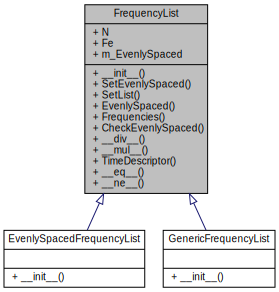
\includegraphics[width=350pt]{classSignalIntegrity_1_1FrequencyDomain_1_1FrequencyList_1_1FrequencyList__inherit__graph}
\end{center}
\end{figure}


Collaboration diagram for Frequency\+List\+:\nopagebreak
\begin{figure}[H]
\begin{center}
\leavevmode
\includegraphics[width=203pt]{classSignalIntegrity_1_1FrequencyDomain_1_1FrequencyList_1_1FrequencyList__coll__graph}
\end{center}
\end{figure}
\subsection*{Public Member Functions}
\begin{DoxyCompactItemize}
\item 
def \hyperlink{classSignalIntegrity_1_1FrequencyDomain_1_1FrequencyList_1_1FrequencyList_a8e9ec4f7f7796f2f07894cd60aeecdcd}{\+\_\+\+\_\+init\+\_\+\+\_\+} (self, f=None)
\begin{DoxyCompactList}\small\item\em Constructor. \end{DoxyCompactList}\item 
def \hyperlink{classSignalIntegrity_1_1FrequencyDomain_1_1FrequencyList_1_1FrequencyList_a910c951aef6578c9e467ddef68c94539}{Set\+Evenly\+Spaced} (self, \hyperlink{classSignalIntegrity_1_1FrequencyDomain_1_1FrequencyList_1_1FrequencyList_a7313483ea19e09cf50b8b58d531b871d}{Fe}, \hyperlink{classSignalIntegrity_1_1FrequencyDomain_1_1FrequencyList_1_1FrequencyList_a8cc2e7240164328fdc3f0e5e21032c56}{N})
\begin{DoxyCompactList}\small\item\em sets evenly spaced \end{DoxyCompactList}\item 
def \hyperlink{classSignalIntegrity_1_1FrequencyDomain_1_1FrequencyList_1_1FrequencyList_a23f5bda3ad522bcdc1af831f4178ddca}{Set\+List} (self, fl)
\begin{DoxyCompactList}\small\item\em Initializes the frequency list with a list of frequencies. \end{DoxyCompactList}\item 
def \hyperlink{classSignalIntegrity_1_1FrequencyDomain_1_1FrequencyList_1_1FrequencyList_a3f206c8bc15662bf50b9d889b9870c0d}{Evenly\+Spaced} (self)
\begin{DoxyCompactList}\small\item\em whether evenly spaced \end{DoxyCompactList}\item 
def \hyperlink{classSignalIntegrity_1_1FrequencyDomain_1_1FrequencyList_1_1FrequencyList_a227f355ed05bff8c1061e26a8a53758a}{Frequencies} (self, unit=None)
\begin{DoxyCompactList}\small\item\em Frequencies. \end{DoxyCompactList}\item 
def \hyperlink{classSignalIntegrity_1_1FrequencyDomain_1_1FrequencyList_1_1FrequencyList_a903469a93e04d2e4604e4350f2096a2d}{Check\+Evenly\+Spaced} (self, epsilon=0.\+01)
\begin{DoxyCompactList}\small\item\em checks and sets whether evenly spaced \end{DoxyCompactList}\item 
def \hyperlink{classSignalIntegrity_1_1FrequencyDomain_1_1FrequencyList_1_1FrequencyList_a5780a728adfb401a59d29d748b4abf91}{\+\_\+\+\_\+div\+\_\+\+\_\+} (self, d)
\begin{DoxyCompactList}\small\item\em overloads / \end{DoxyCompactList}\item 
def \hyperlink{classSignalIntegrity_1_1FrequencyDomain_1_1FrequencyList_1_1FrequencyList_a07c88d52e0963bb0c56e013184cd0d24}{\+\_\+\+\_\+mul\+\_\+\+\_\+} (self, d)
\begin{DoxyCompactList}\small\item\em overloads $\ast$ \end{DoxyCompactList}\item 
def \hyperlink{classSignalIntegrity_1_1FrequencyDomain_1_1FrequencyList_1_1FrequencyList_ae0cb8207edfbc631f1af2fc543e3d4d7}{Time\+Descriptor} (self, Keven=True)
\begin{DoxyCompactList}\small\item\em associated time descriptor \end{DoxyCompactList}\item 
def \hyperlink{classSignalIntegrity_1_1FrequencyDomain_1_1FrequencyList_1_1FrequencyList_ad794ff077f2f05f228a7109f3670ac40}{\+\_\+\+\_\+eq\+\_\+\+\_\+} (self, other)
\begin{DoxyCompactList}\small\item\em overloads == \end{DoxyCompactList}\item 
def \hyperlink{classSignalIntegrity_1_1FrequencyDomain_1_1FrequencyList_1_1FrequencyList_aa0b54a20b36fcc55e1147de88d083072}{\+\_\+\+\_\+ne\+\_\+\+\_\+} (self, other)
\begin{DoxyCompactList}\small\item\em overloads != \end{DoxyCompactList}\end{DoxyCompactItemize}
\subsection*{Public Attributes}
\begin{DoxyCompactItemize}
\item 
\hyperlink{classSignalIntegrity_1_1FrequencyDomain_1_1FrequencyList_1_1FrequencyList_a8cc2e7240164328fdc3f0e5e21032c56}{N}
\begin{DoxyCompactList}\small\item\em integer number (-\/1) of frequency list elements (i.\+e. \end{DoxyCompactList}\item 
\mbox{\Hypertarget{classSignalIntegrity_1_1FrequencyDomain_1_1FrequencyList_1_1FrequencyList_a7313483ea19e09cf50b8b58d531b871d}\label{classSignalIntegrity_1_1FrequencyDomain_1_1FrequencyList_1_1FrequencyList_a7313483ea19e09cf50b8b58d531b871d}} 
\hyperlink{classSignalIntegrity_1_1FrequencyDomain_1_1FrequencyList_1_1FrequencyList_a7313483ea19e09cf50b8b58d531b871d}{Fe}
\begin{DoxyCompactList}\small\item\em float end frequency for the frequency list \end{DoxyCompactList}\item 
\mbox{\Hypertarget{classSignalIntegrity_1_1FrequencyDomain_1_1FrequencyList_1_1FrequencyList_a2d85a36e030819ea57fb06cdb76e90c4}\label{classSignalIntegrity_1_1FrequencyDomain_1_1FrequencyList_1_1FrequencyList_a2d85a36e030819ea57fb06cdb76e90c4}} 
\hyperlink{classSignalIntegrity_1_1FrequencyDomain_1_1FrequencyList_1_1FrequencyList_a2d85a36e030819ea57fb06cdb76e90c4}{m\+\_\+\+Evenly\+Spaced}
\begin{DoxyCompactList}\small\item\em boolean whether the list of frequencies is evenly spaced \end{DoxyCompactList}\end{DoxyCompactItemize}


\subsection{Detailed Description}
Frequency lists. 

Deals efficiently with evenly spaced frequency lists that can be described by three simple numbers and unvenly spaced freqeuncy lists that must contain the list of frequencies themselves. Not only can evenly spaced frequency lists be compressed in data size, we often must know if the frequencies are evenly spaced and it\textquotesingle{}s easier to know that when it is that class type.

Teledyne Le\+Croy Inc. (\char`\"{}\+C\+O\+M\+P\+A\+N\+Y\char`\"{}) C\+O\+N\+F\+I\+D\+E\+N\+T\+I\+AL Unpublished Copyright (c) 2015-\/2016 Peter J. Pupalaikis and Teledyne Le\+Croy, All Rights Reserved.

Explicit license in accompanying R\+E\+A\+D\+M\+E.\+txt file. If you don\textquotesingle{}t have that file or do not agree to the terms in that file, then you are not licensed to use this material whatsoever. base class for lists of frequencies. 

Definition at line 22 of file Frequency\+List.\+py.



\subsection{Constructor \& Destructor Documentation}
\mbox{\Hypertarget{classSignalIntegrity_1_1FrequencyDomain_1_1FrequencyList_1_1FrequencyList_a8e9ec4f7f7796f2f07894cd60aeecdcd}\label{classSignalIntegrity_1_1FrequencyDomain_1_1FrequencyList_1_1FrequencyList_a8e9ec4f7f7796f2f07894cd60aeecdcd}} 
\index{Signal\+Integrity\+::\+Frequency\+Domain\+::\+Frequency\+List\+::\+Frequency\+List@{Signal\+Integrity\+::\+Frequency\+Domain\+::\+Frequency\+List\+::\+Frequency\+List}!\+\_\+\+\_\+init\+\_\+\+\_\+@{\+\_\+\+\_\+init\+\_\+\+\_\+}}
\index{\+\_\+\+\_\+init\+\_\+\+\_\+@{\+\_\+\+\_\+init\+\_\+\+\_\+}!Signal\+Integrity\+::\+Frequency\+Domain\+::\+Frequency\+List\+::\+Frequency\+List@{Signal\+Integrity\+::\+Frequency\+Domain\+::\+Frequency\+List\+::\+Frequency\+List}}
\subsubsection{\texorpdfstring{\+\_\+\+\_\+init\+\_\+\+\_\+()}{\_\_init\_\_()}}
{\footnotesize\ttfamily def \+\_\+\+\_\+init\+\_\+\+\_\+ (\begin{DoxyParamCaption}\item[{}]{self,  }\item[{}]{f = {\ttfamily None} }\end{DoxyParamCaption})}



Constructor. 

Initializes a frequency list either from another frequency list or from a list of frequencies provided. 
\begin{DoxyParams}{Parameters}
{\em f} & (optional) list of frequencies or instance of class \hyperlink{classSignalIntegrity_1_1FrequencyDomain_1_1FrequencyList_1_1FrequencyList}{Frequency\+List} \\
\hline
\end{DoxyParams}


Definition at line 30 of file Frequency\+List.\+py.



\subsection{Member Function Documentation}
\mbox{\Hypertarget{classSignalIntegrity_1_1FrequencyDomain_1_1FrequencyList_1_1FrequencyList_a5780a728adfb401a59d29d748b4abf91}\label{classSignalIntegrity_1_1FrequencyDomain_1_1FrequencyList_1_1FrequencyList_a5780a728adfb401a59d29d748b4abf91}} 
\index{Signal\+Integrity\+::\+Frequency\+Domain\+::\+Frequency\+List\+::\+Frequency\+List@{Signal\+Integrity\+::\+Frequency\+Domain\+::\+Frequency\+List\+::\+Frequency\+List}!\+\_\+\+\_\+div\+\_\+\+\_\+@{\+\_\+\+\_\+div\+\_\+\+\_\+}}
\index{\+\_\+\+\_\+div\+\_\+\+\_\+@{\+\_\+\+\_\+div\+\_\+\+\_\+}!Signal\+Integrity\+::\+Frequency\+Domain\+::\+Frequency\+List\+::\+Frequency\+List@{Signal\+Integrity\+::\+Frequency\+Domain\+::\+Frequency\+List\+::\+Frequency\+List}}
\subsubsection{\texorpdfstring{\+\_\+\+\_\+div\+\_\+\+\_\+()}{\_\_div\_\_()}}
{\footnotesize\ttfamily def \+\_\+\+\_\+div\+\_\+\+\_\+ (\begin{DoxyParamCaption}\item[{}]{self,  }\item[{}]{d }\end{DoxyParamCaption})}



overloads / 


\begin{DoxyParams}{Parameters}
{\em d} & float frequency to divide each frequency by. \\
\hline
\end{DoxyParams}
\begin{DoxyReturn}{Returns}
an instance of class \hyperlink{classSignalIntegrity_1_1FrequencyDomain_1_1FrequencyList_1_1FrequencyList}{Frequency\+List} containing self divided by the amount specified. 
\end{DoxyReturn}


Definition at line 126 of file Frequency\+List.\+py.

\mbox{\Hypertarget{classSignalIntegrity_1_1FrequencyDomain_1_1FrequencyList_1_1FrequencyList_ad794ff077f2f05f228a7109f3670ac40}\label{classSignalIntegrity_1_1FrequencyDomain_1_1FrequencyList_1_1FrequencyList_ad794ff077f2f05f228a7109f3670ac40}} 
\index{Signal\+Integrity\+::\+Frequency\+Domain\+::\+Frequency\+List\+::\+Frequency\+List@{Signal\+Integrity\+::\+Frequency\+Domain\+::\+Frequency\+List\+::\+Frequency\+List}!\+\_\+\+\_\+eq\+\_\+\+\_\+@{\+\_\+\+\_\+eq\+\_\+\+\_\+}}
\index{\+\_\+\+\_\+eq\+\_\+\+\_\+@{\+\_\+\+\_\+eq\+\_\+\+\_\+}!Signal\+Integrity\+::\+Frequency\+Domain\+::\+Frequency\+List\+::\+Frequency\+List@{Signal\+Integrity\+::\+Frequency\+Domain\+::\+Frequency\+List\+::\+Frequency\+List}}
\subsubsection{\texorpdfstring{\+\_\+\+\_\+eq\+\_\+\+\_\+()}{\_\_eq\_\_()}}
{\footnotesize\ttfamily def \+\_\+\+\_\+eq\+\_\+\+\_\+ (\begin{DoxyParamCaption}\item[{}]{self,  }\item[{}]{other }\end{DoxyParamCaption})}



overloads == 


\begin{DoxyParams}{Parameters}
{\em other} & an other instance of class \hyperlink{classSignalIntegrity_1_1FrequencyDomain_1_1FrequencyList_1_1FrequencyList}{Frequency\+List} \\
\hline
\end{DoxyParams}
\begin{DoxyReturn}{Returns}
boolean True if the other is the same as self. 
\end{DoxyReturn}
\begin{DoxyNote}{Note}
the elements in the list are checked within an epsilon value of 1e-\/6. 
\end{DoxyNote}


Definition at line 165 of file Frequency\+List.\+py.

\mbox{\Hypertarget{classSignalIntegrity_1_1FrequencyDomain_1_1FrequencyList_1_1FrequencyList_a07c88d52e0963bb0c56e013184cd0d24}\label{classSignalIntegrity_1_1FrequencyDomain_1_1FrequencyList_1_1FrequencyList_a07c88d52e0963bb0c56e013184cd0d24}} 
\index{Signal\+Integrity\+::\+Frequency\+Domain\+::\+Frequency\+List\+::\+Frequency\+List@{Signal\+Integrity\+::\+Frequency\+Domain\+::\+Frequency\+List\+::\+Frequency\+List}!\+\_\+\+\_\+mul\+\_\+\+\_\+@{\+\_\+\+\_\+mul\+\_\+\+\_\+}}
\index{\+\_\+\+\_\+mul\+\_\+\+\_\+@{\+\_\+\+\_\+mul\+\_\+\+\_\+}!Signal\+Integrity\+::\+Frequency\+Domain\+::\+Frequency\+List\+::\+Frequency\+List@{Signal\+Integrity\+::\+Frequency\+Domain\+::\+Frequency\+List\+::\+Frequency\+List}}
\subsubsection{\texorpdfstring{\+\_\+\+\_\+mul\+\_\+\+\_\+()}{\_\_mul\_\_()}}
{\footnotesize\ttfamily def \+\_\+\+\_\+mul\+\_\+\+\_\+ (\begin{DoxyParamCaption}\item[{}]{self,  }\item[{}]{d }\end{DoxyParamCaption})}



overloads $\ast$ 


\begin{DoxyParams}{Parameters}
{\em d} & float frequency to multiply each frequency by. \\
\hline
\end{DoxyParams}
\begin{DoxyReturn}{Returns}
an instance of class \hyperlink{classSignalIntegrity_1_1FrequencyDomain_1_1FrequencyList_1_1FrequencyList}{Frequency\+List} containing self multiplied by the amount specified. 
\end{DoxyReturn}


Definition at line 136 of file Frequency\+List.\+py.

\mbox{\Hypertarget{classSignalIntegrity_1_1FrequencyDomain_1_1FrequencyList_1_1FrequencyList_aa0b54a20b36fcc55e1147de88d083072}\label{classSignalIntegrity_1_1FrequencyDomain_1_1FrequencyList_1_1FrequencyList_aa0b54a20b36fcc55e1147de88d083072}} 
\index{Signal\+Integrity\+::\+Frequency\+Domain\+::\+Frequency\+List\+::\+Frequency\+List@{Signal\+Integrity\+::\+Frequency\+Domain\+::\+Frequency\+List\+::\+Frequency\+List}!\+\_\+\+\_\+ne\+\_\+\+\_\+@{\+\_\+\+\_\+ne\+\_\+\+\_\+}}
\index{\+\_\+\+\_\+ne\+\_\+\+\_\+@{\+\_\+\+\_\+ne\+\_\+\+\_\+}!Signal\+Integrity\+::\+Frequency\+Domain\+::\+Frequency\+List\+::\+Frequency\+List@{Signal\+Integrity\+::\+Frequency\+Domain\+::\+Frequency\+List\+::\+Frequency\+List}}
\subsubsection{\texorpdfstring{\+\_\+\+\_\+ne\+\_\+\+\_\+()}{\_\_ne\_\_()}}
{\footnotesize\ttfamily def \+\_\+\+\_\+ne\+\_\+\+\_\+ (\begin{DoxyParamCaption}\item[{}]{self,  }\item[{}]{other }\end{DoxyParamCaption})}



overloads != 


\begin{DoxyParams}{Parameters}
{\em other} & an other instance of class \hyperlink{classSignalIntegrity_1_1FrequencyDomain_1_1FrequencyList_1_1FrequencyList}{Frequency\+List} \\
\hline
\end{DoxyParams}
\begin{DoxyReturn}{Returns}
boolean True if the other is the same as self. 
\end{DoxyReturn}
\begin{DoxySeeAlso}{See also}
{\bfseries eq}() 
\end{DoxySeeAlso}


Definition at line 183 of file Frequency\+List.\+py.

\mbox{\Hypertarget{classSignalIntegrity_1_1FrequencyDomain_1_1FrequencyList_1_1FrequencyList_a903469a93e04d2e4604e4350f2096a2d}\label{classSignalIntegrity_1_1FrequencyDomain_1_1FrequencyList_1_1FrequencyList_a903469a93e04d2e4604e4350f2096a2d}} 
\index{Signal\+Integrity\+::\+Frequency\+Domain\+::\+Frequency\+List\+::\+Frequency\+List@{Signal\+Integrity\+::\+Frequency\+Domain\+::\+Frequency\+List\+::\+Frequency\+List}!Check\+Evenly\+Spaced@{Check\+Evenly\+Spaced}}
\index{Check\+Evenly\+Spaced@{Check\+Evenly\+Spaced}!Signal\+Integrity\+::\+Frequency\+Domain\+::\+Frequency\+List\+::\+Frequency\+List@{Signal\+Integrity\+::\+Frequency\+Domain\+::\+Frequency\+List\+::\+Frequency\+List}}
\subsubsection{\texorpdfstring{Check\+Evenly\+Spaced()}{CheckEvenlySpaced()}}
{\footnotesize\ttfamily def Check\+Evenly\+Spaced (\begin{DoxyParamCaption}\item[{}]{self,  }\item[{}]{epsilon = {\ttfamily 0.01} }\end{DoxyParamCaption})}



checks and sets whether evenly spaced 


\begin{DoxyParams}{Parameters}
{\em epsilon} & (optional) float difference tolerated in whether a frequency compared is the same. (Defaults to 0.\+01). \\
\hline
\end{DoxyParams}
\begin{DoxyReturn}{Returns}
boolean whether the frequency list is evenly spaced. 
\end{DoxyReturn}
\begin{DoxyNote}{Note}
if the m\+\_\+\+Evenly\+Spaced internal variable indicates it\textquotesingle{}s evenly spaced, it simply returns True.
\end{DoxyNote}
Checks the frequencies to see if they conform to N+1 frequencies with for n=0..N, each frequency in the list is f\mbox{[}n\mbox{]}=n/\+N$\ast$\+Fe within the epsilon. 

Definition at line 112 of file Frequency\+List.\+py.

\mbox{\Hypertarget{classSignalIntegrity_1_1FrequencyDomain_1_1FrequencyList_1_1FrequencyList_a3f206c8bc15662bf50b9d889b9870c0d}\label{classSignalIntegrity_1_1FrequencyDomain_1_1FrequencyList_1_1FrequencyList_a3f206c8bc15662bf50b9d889b9870c0d}} 
\index{Signal\+Integrity\+::\+Frequency\+Domain\+::\+Frequency\+List\+::\+Frequency\+List@{Signal\+Integrity\+::\+Frequency\+Domain\+::\+Frequency\+List\+::\+Frequency\+List}!Evenly\+Spaced@{Evenly\+Spaced}}
\index{Evenly\+Spaced@{Evenly\+Spaced}!Signal\+Integrity\+::\+Frequency\+Domain\+::\+Frequency\+List\+::\+Frequency\+List@{Signal\+Integrity\+::\+Frequency\+Domain\+::\+Frequency\+List\+::\+Frequency\+List}}
\subsubsection{\texorpdfstring{Evenly\+Spaced()}{EvenlySpaced()}}
{\footnotesize\ttfamily def Evenly\+Spaced (\begin{DoxyParamCaption}\item[{}]{self }\end{DoxyParamCaption})}



whether evenly spaced 

\begin{DoxyReturn}{Returns}
boolean whether the list is evenly spaced. 
\end{DoxyReturn}
\begin{DoxyNote}{Note}
It checks this by examining the internal flag m\+\_\+\+Evenly\+Spaced. It does no actual check of the list of frequencies. 
\end{DoxyNote}


Definition at line 76 of file Frequency\+List.\+py.

\mbox{\Hypertarget{classSignalIntegrity_1_1FrequencyDomain_1_1FrequencyList_1_1FrequencyList_a227f355ed05bff8c1061e26a8a53758a}\label{classSignalIntegrity_1_1FrequencyDomain_1_1FrequencyList_1_1FrequencyList_a227f355ed05bff8c1061e26a8a53758a}} 
\index{Signal\+Integrity\+::\+Frequency\+Domain\+::\+Frequency\+List\+::\+Frequency\+List@{Signal\+Integrity\+::\+Frequency\+Domain\+::\+Frequency\+List\+::\+Frequency\+List}!Frequencies@{Frequencies}}
\index{Frequencies@{Frequencies}!Signal\+Integrity\+::\+Frequency\+Domain\+::\+Frequency\+List\+::\+Frequency\+List@{Signal\+Integrity\+::\+Frequency\+Domain\+::\+Frequency\+List\+::\+Frequency\+List}}
\subsubsection{\texorpdfstring{Frequencies()}{Frequencies()}}
{\footnotesize\ttfamily def Frequencies (\begin{DoxyParamCaption}\item[{}]{self,  }\item[{}]{unit = {\ttfamily None} }\end{DoxyParamCaption})}



Frequencies. 


\begin{DoxyParams}{Parameters}
{\em unit} & optional string containing unit to use \\
\hline
\end{DoxyParams}
\begin{DoxyReturn}{Returns}
list of frequencies in the frequency list in the unit specified 
\end{DoxyReturn}
\begin{DoxyRemark}{Remarks}
Valid units are\+:
\begin{DoxyItemize}
\item G\+Hz -\/ each frequency element is divided by 1e9.
\item M\+Hz -\/ each frequency element is divided by 1e6.
\item k\+Hz -\/ each frequency element is divided by 1e3
\end{DoxyItemize}
\end{DoxyRemark}
If no unit is supplied or if it\textquotesingle{}s None, then the frequencies are provided as is.

if the unit supplied is otherwise invalid, None is returned. 

Definition at line 91 of file Frequency\+List.\+py.

\mbox{\Hypertarget{classSignalIntegrity_1_1FrequencyDomain_1_1FrequencyList_1_1FrequencyList_a910c951aef6578c9e467ddef68c94539}\label{classSignalIntegrity_1_1FrequencyDomain_1_1FrequencyList_1_1FrequencyList_a910c951aef6578c9e467ddef68c94539}} 
\index{Signal\+Integrity\+::\+Frequency\+Domain\+::\+Frequency\+List\+::\+Frequency\+List@{Signal\+Integrity\+::\+Frequency\+Domain\+::\+Frequency\+List\+::\+Frequency\+List}!Set\+Evenly\+Spaced@{Set\+Evenly\+Spaced}}
\index{Set\+Evenly\+Spaced@{Set\+Evenly\+Spaced}!Signal\+Integrity\+::\+Frequency\+Domain\+::\+Frequency\+List\+::\+Frequency\+List@{Signal\+Integrity\+::\+Frequency\+Domain\+::\+Frequency\+List\+::\+Frequency\+List}}
\subsubsection{\texorpdfstring{Set\+Evenly\+Spaced()}{SetEvenlySpaced()}}
{\footnotesize\ttfamily def Set\+Evenly\+Spaced (\begin{DoxyParamCaption}\item[{}]{self,  }\item[{}]{Fe,  }\item[{}]{N }\end{DoxyParamCaption})}



sets evenly spaced 


\begin{DoxyParams}{Parameters}
{\em Fe} & float end frequency for the frequency list \\
\hline
{\em N} & integer number of points (-\/1) or the frequency list (i.\+e. the number of points in the new frequency list will be N+1. \\
\hline
\end{DoxyParams}
\begin{DoxyReturn}{Returns}
self 
\end{DoxyReturn}
\begin{DoxyRemark}{Remarks}
Initializes the frequency list to be evenly spaced with N+1 points from n=0..N where each frequency is f\mbox{[}n\mbox{]}=n/\+N$\ast$\+Fe 
\end{DoxyRemark}


Definition at line 47 of file Frequency\+List.\+py.

\mbox{\Hypertarget{classSignalIntegrity_1_1FrequencyDomain_1_1FrequencyList_1_1FrequencyList_a23f5bda3ad522bcdc1af831f4178ddca}\label{classSignalIntegrity_1_1FrequencyDomain_1_1FrequencyList_1_1FrequencyList_a23f5bda3ad522bcdc1af831f4178ddca}} 
\index{Signal\+Integrity\+::\+Frequency\+Domain\+::\+Frequency\+List\+::\+Frequency\+List@{Signal\+Integrity\+::\+Frequency\+Domain\+::\+Frequency\+List\+::\+Frequency\+List}!Set\+List@{Set\+List}}
\index{Set\+List@{Set\+List}!Signal\+Integrity\+::\+Frequency\+Domain\+::\+Frequency\+List\+::\+Frequency\+List@{Signal\+Integrity\+::\+Frequency\+Domain\+::\+Frequency\+List\+::\+Frequency\+List}}
\subsubsection{\texorpdfstring{Set\+List()}{SetList()}}
{\footnotesize\ttfamily def Set\+List (\begin{DoxyParamCaption}\item[{}]{self,  }\item[{}]{fl }\end{DoxyParamCaption})}



Initializes the frequency list with a list of frequencies. 


\begin{DoxyParams}{Parameters}
{\em fl} & list of frequencies \\
\hline
\end{DoxyParams}
\begin{DoxyReturn}{Returns}
self 
\end{DoxyReturn}
\begin{DoxyRemark}{Remarks}
This will set the List to the list provided, N to the length -\/1, and Fe to the frequency of the last element in the list. It will set m\+\_\+\+Evenly\+Spaced False. 
\end{DoxyRemark}
\begin{DoxyNote}{Note}
although this initializer is meant to take a list of frequencies, it will also take an instance of class \hyperlink{classSignalIntegrity_1_1FrequencyDomain_1_1FrequencyList_1_1FrequencyList}{Frequency\+List}, as it mimics this list behavior. In this case, it will install it as if the \hyperlink{classSignalIntegrity_1_1FrequencyDomain_1_1FrequencyList_1_1FrequencyList}{Frequency\+List} instance was simply a list of frequencies. 
\end{DoxyNote}


Definition at line 64 of file Frequency\+List.\+py.

\mbox{\Hypertarget{classSignalIntegrity_1_1FrequencyDomain_1_1FrequencyList_1_1FrequencyList_ae0cb8207edfbc631f1af2fc543e3d4d7}\label{classSignalIntegrity_1_1FrequencyDomain_1_1FrequencyList_1_1FrequencyList_ae0cb8207edfbc631f1af2fc543e3d4d7}} 
\index{Signal\+Integrity\+::\+Frequency\+Domain\+::\+Frequency\+List\+::\+Frequency\+List@{Signal\+Integrity\+::\+Frequency\+Domain\+::\+Frequency\+List\+::\+Frequency\+List}!Time\+Descriptor@{Time\+Descriptor}}
\index{Time\+Descriptor@{Time\+Descriptor}!Signal\+Integrity\+::\+Frequency\+Domain\+::\+Frequency\+List\+::\+Frequency\+List@{Signal\+Integrity\+::\+Frequency\+Domain\+::\+Frequency\+List\+::\+Frequency\+List}}
\subsubsection{\texorpdfstring{Time\+Descriptor()}{TimeDescriptor()}}
{\footnotesize\ttfamily def \hyperlink{classSignalIntegrity_1_1TimeDomain_1_1Waveform_1_1TimeDescriptor_1_1TimeDescriptor}{Time\+Descriptor} (\begin{DoxyParamCaption}\item[{}]{self,  }\item[{}]{Keven = {\ttfamily True} }\end{DoxyParamCaption})}



associated time descriptor 


\begin{DoxyParams}{Parameters}
{\em Keven} & boolean (optional) Whether N is from an even K points in the time domain (i.\+e. K/2) or from an odd K points in the time-\/domain (i.\+e. (K+1)/2). Defaults to True. \\
\hline
\end{DoxyParams}
\begin{DoxyReturn}{Returns}
an instance of class Time\+Descriptor that corresponds to the time descriptor that would generate this frequency descriptor. 
\end{DoxyReturn}
\begin{DoxyNote}{Note}
this is assumed to be a time descriptor that would produce a frequency descriptor with self\textquotesingle{}s end frequency and number of points. It does not check whether the list is evenly spaced. 
\end{DoxyNote}


Definition at line 150 of file Frequency\+List.\+py.



\subsection{Member Data Documentation}
\mbox{\Hypertarget{classSignalIntegrity_1_1FrequencyDomain_1_1FrequencyList_1_1FrequencyList_a8cc2e7240164328fdc3f0e5e21032c56}\label{classSignalIntegrity_1_1FrequencyDomain_1_1FrequencyList_1_1FrequencyList_a8cc2e7240164328fdc3f0e5e21032c56}} 
\index{Signal\+Integrity\+::\+Frequency\+Domain\+::\+Frequency\+List\+::\+Frequency\+List@{Signal\+Integrity\+::\+Frequency\+Domain\+::\+Frequency\+List\+::\+Frequency\+List}!N@{N}}
\index{N@{N}!Signal\+Integrity\+::\+Frequency\+Domain\+::\+Frequency\+List\+::\+Frequency\+List@{Signal\+Integrity\+::\+Frequency\+Domain\+::\+Frequency\+List\+::\+Frequency\+List}}
\subsubsection{\texorpdfstring{N}{N}}
{\footnotesize\ttfamily N}



integer number (-\/1) of frequency list elements (i.\+e. 

the number of frequency elements is N+1. 

Definition at line 33 of file Frequency\+List.\+py.



The documentation for this class was generated from the following file\+:\begin{DoxyCompactItemize}
\item 
Py\+S\+I/\+Signal\+Integrity/\+Frequency\+Domain/Frequency\+List.\+py\end{DoxyCompactItemize}

\hypertarget{classSignalIntegrity_1_1FrequencyDomain_1_1FrequencyResponse_1_1FrequencyResponse}{}\section{Frequency\+Response Class Reference}
\label{classSignalIntegrity_1_1FrequencyDomain_1_1FrequencyResponse_1_1FrequencyResponse}\index{Frequency\+Response@{Frequency\+Response}}


\hyperlink{classSignalIntegrity_1_1FrequencyDomain_1_1FrequencyResponse_1_1FrequencyResponse}{Frequency\+Response}.  




Inheritance diagram for Frequency\+Response\+:
\nopagebreak
\begin{figure}[H]
\begin{center}
\leavevmode
\includegraphics[width=190pt]{classSignalIntegrity_1_1FrequencyDomain_1_1FrequencyResponse_1_1FrequencyResponse__inherit__graph}
\end{center}
\end{figure}


Collaboration diagram for Frequency\+Response\+:
\nopagebreak
\begin{figure}[H]
\begin{center}
\leavevmode
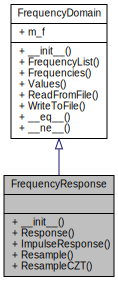
\includegraphics[width=190pt]{classSignalIntegrity_1_1FrequencyDomain_1_1FrequencyResponse_1_1FrequencyResponse__coll__graph}
\end{center}
\end{figure}
\subsection*{Public Member Functions}
\begin{DoxyCompactItemize}
\item 
def \hyperlink{classSignalIntegrity_1_1FrequencyDomain_1_1FrequencyResponse_1_1FrequencyResponse_af89c1b84b55a8388acf19c91be67a97e}{\+\_\+\+\_\+init\+\_\+\+\_\+} (self, f=None, resp=None)
\begin{DoxyCompactList}\small\item\em Constructor. \end{DoxyCompactList}\item 
def \hyperlink{classSignalIntegrity_1_1FrequencyDomain_1_1FrequencyResponse_1_1FrequencyResponse_ab4996cceccaa974296395d3039a9ca2a}{Response} (self, unit=None)
\begin{DoxyCompactList}\small\item\em Response. \end{DoxyCompactList}\item 
def \hyperlink{classSignalIntegrity_1_1FrequencyDomain_1_1FrequencyResponse_1_1FrequencyResponse_aa301152e06c3881589eb5c70d53734f6}{Impulse\+Response} (self, td=None, adjust\+Delay=True)
\begin{DoxyCompactList}\small\item\em the time-\/domain impulse response \end{DoxyCompactList}\item 
def \hyperlink{classSignalIntegrity_1_1FrequencyDomain_1_1FrequencyResponse_1_1FrequencyResponse_a6aa7e8bdecb4f17e41d783d00a27fdd8}{Resample} (self, fdp)
\begin{DoxyCompactList}\small\item\em Resamples to a different set of frequencies. \end{DoxyCompactList}\item 
def \hyperlink{classSignalIntegrity_1_1FrequencyDomain_1_1FrequencyResponse_1_1FrequencyResponse_af61ffacaaef319b5b0752778bfe522e6}{Resample\+C\+ZT} (self, fdp, speedy=True)
\begin{DoxyCompactList}\small\item\em Uses the chirp z transform is used to resample. \end{DoxyCompactList}\end{DoxyCompactItemize}
\subsection*{Additional Inherited Members}


\subsection{Detailed Description}
\hyperlink{classSignalIntegrity_1_1FrequencyDomain_1_1FrequencyResponse_1_1FrequencyResponse}{Frequency\+Response}. 

Frequency response view of a waveform assumed computed from the Frequency\+Response() method of a class Impulse\+Response, which is itself derived from the class Waveform. In other words, it would contain complex frequency-\/domain values that, if multiplied by the values in an instance of class \hyperlink{namespaceSignalIntegrity_1_1FrequencyDomain_1_1FrequencyContent}{Frequency\+Content}, would filter the waveform in the frequency-\/domain. \begin{DoxySeeAlso}{See also}
\hyperlink{classSignalIntegrity_1_1FrequencyDomain_1_1FrequencyResponse_1_1FrequencyResponse_aa301152e06c3881589eb5c70d53734f6}{Impulse\+Response} 
\end{DoxySeeAlso}


Definition at line 42 of file Frequency\+Response.\+py.



\subsection{Constructor \& Destructor Documentation}
\mbox{\Hypertarget{classSignalIntegrity_1_1FrequencyDomain_1_1FrequencyResponse_1_1FrequencyResponse_af89c1b84b55a8388acf19c91be67a97e}\label{classSignalIntegrity_1_1FrequencyDomain_1_1FrequencyResponse_1_1FrequencyResponse_af89c1b84b55a8388acf19c91be67a97e}} 
\index{Signal\+Integrity\+::\+Frequency\+Domain\+::\+Frequency\+Response\+::\+Frequency\+Response@{Signal\+Integrity\+::\+Frequency\+Domain\+::\+Frequency\+Response\+::\+Frequency\+Response}!\+\_\+\+\_\+init\+\_\+\+\_\+@{\+\_\+\+\_\+init\+\_\+\+\_\+}}
\index{\+\_\+\+\_\+init\+\_\+\+\_\+@{\+\_\+\+\_\+init\+\_\+\+\_\+}!Signal\+Integrity\+::\+Frequency\+Domain\+::\+Frequency\+Response\+::\+Frequency\+Response@{Signal\+Integrity\+::\+Frequency\+Domain\+::\+Frequency\+Response\+::\+Frequency\+Response}}
\subsubsection{\texorpdfstring{\+\_\+\+\_\+init\+\_\+\+\_\+()}{\_\_init\_\_()}}
{\footnotesize\ttfamily def \+\_\+\+\_\+init\+\_\+\+\_\+ (\begin{DoxyParamCaption}\item[{}]{self,  }\item[{}]{f = {\ttfamily None},  }\item[{}]{resp = {\ttfamily None} }\end{DoxyParamCaption})}



Constructor. 


\begin{DoxyParams}{Parameters}
{\em f} & instance of class \hyperlink{namespaceSignalIntegrity_1_1FrequencyDomain_1_1FrequencyList}{Frequency\+List} \\
\hline
{\em resp} & list of complex values \\
\hline
\end{DoxyParams}
\begin{DoxyRemark}{Remarks}
It is assumed that the frequencies and the response provided were generated from the Frequency\+Response() method of the class Impulse\+Response. 
\end{DoxyRemark}


Definition at line 50 of file Frequency\+Response.\+py.



\subsection{Member Function Documentation}
\mbox{\Hypertarget{classSignalIntegrity_1_1FrequencyDomain_1_1FrequencyResponse_1_1FrequencyResponse_aa301152e06c3881589eb5c70d53734f6}\label{classSignalIntegrity_1_1FrequencyDomain_1_1FrequencyResponse_1_1FrequencyResponse_aa301152e06c3881589eb5c70d53734f6}} 
\index{Signal\+Integrity\+::\+Frequency\+Domain\+::\+Frequency\+Response\+::\+Frequency\+Response@{Signal\+Integrity\+::\+Frequency\+Domain\+::\+Frequency\+Response\+::\+Frequency\+Response}!Impulse\+Response@{Impulse\+Response}}
\index{Impulse\+Response@{Impulse\+Response}!Signal\+Integrity\+::\+Frequency\+Domain\+::\+Frequency\+Response\+::\+Frequency\+Response@{Signal\+Integrity\+::\+Frequency\+Domain\+::\+Frequency\+Response\+::\+Frequency\+Response}}
\subsubsection{\texorpdfstring{Impulse\+Response()}{ImpulseResponse()}}
{\footnotesize\ttfamily def \hyperlink{classSignalIntegrity_1_1TimeDomain_1_1Waveform_1_1ImpulseResponse_1_1ImpulseResponse}{Impulse\+Response} (\begin{DoxyParamCaption}\item[{}]{self,  }\item[{}]{td = {\ttfamily None},  }\item[{}]{adjust\+Delay = {\ttfamily True} }\end{DoxyParamCaption})}



the time-\/domain impulse response 


\begin{DoxyParams}{Parameters}
{\em td} & (optional) instance of class Time\+Descriptor. \\
\hline
{\em adjust\+Delay} & (optional) bool whether to adjust the delay. \\
\hline
\end{DoxyParams}
\begin{DoxyReturn}{Returns}
instance of class Impulse\+Response corresponding to the frequency response. 
\end{DoxyReturn}
\begin{DoxyRemark}{Remarks}
If the optional time descriptor is supplied, the resulting impulse response is resampled onto that time descriptor. 
\end{DoxyRemark}
\begin{DoxyNote}{Note}
internally, the frequency response is either evenly spaced or not.
\end{DoxyNote}
whether evenly spaced, whether a time descriptor is specified and whether to adjust delay determines all possibilities.

\tabulinesep=1mm
\begin{longtabu} spread 0pt [c]{*{4}{|X[-1]}|}
\hline
\rowcolor{\tableheadbgcolor}\PBS\centering \textbf{ evenly spaced }&\PBS\centering \textbf{ time descriptor }&\PBS\centering \textbf{ adjust delay }&\textbf{ Situation  }\\\cline{1-4}
\endfirsthead
\hline
\endfoot
\hline
\rowcolor{\tableheadbgcolor}\PBS\centering \textbf{ evenly spaced }&\PBS\centering \textbf{ time descriptor }&\PBS\centering \textbf{ adjust delay }&\textbf{ Situation  }\\\cline{1-4}
\endhead
\PBS\centering False &\PBS\centering False &\PBS\centering X &Cannot be done \\\cline{1-4}
\PBS\centering False &\PBS\centering True &\PBS\centering X &Spline resamples to time descriptor \\\cline{1-4}
\PBS\centering True &\PBS\centering False &\PBS\centering False &generic impulse response \\\cline{1-4}
\PBS\centering True &\PBS\centering False &\PBS\centering True &impulse response with delay adjusted \\\cline{1-4}
\PBS\centering True &\PBS\centering True &\PBS\centering X &C\+ZT resamples to td -\/ ad forced to T \\\cline{1-4}
\end{longtabu}
Much of these options are meant for internal use. Mostly you should simply use \hyperlink{classSignalIntegrity_1_1FrequencyDomain_1_1FrequencyResponse_1_1FrequencyResponse_aa301152e06c3881589eb5c70d53734f6}{Impulse\+Response()} with the default arguments. 

Definition at line 90 of file Frequency\+Response.\+py.

\mbox{\Hypertarget{classSignalIntegrity_1_1FrequencyDomain_1_1FrequencyResponse_1_1FrequencyResponse_a6aa7e8bdecb4f17e41d783d00a27fdd8}\label{classSignalIntegrity_1_1FrequencyDomain_1_1FrequencyResponse_1_1FrequencyResponse_a6aa7e8bdecb4f17e41d783d00a27fdd8}} 
\index{Signal\+Integrity\+::\+Frequency\+Domain\+::\+Frequency\+Response\+::\+Frequency\+Response@{Signal\+Integrity\+::\+Frequency\+Domain\+::\+Frequency\+Response\+::\+Frequency\+Response}!Resample@{Resample}}
\index{Resample@{Resample}!Signal\+Integrity\+::\+Frequency\+Domain\+::\+Frequency\+Response\+::\+Frequency\+Response@{Signal\+Integrity\+::\+Frequency\+Domain\+::\+Frequency\+Response\+::\+Frequency\+Response}}
\subsubsection{\texorpdfstring{Resample()}{Resample()}}
{\footnotesize\ttfamily def Resample (\begin{DoxyParamCaption}\item[{}]{self,  }\item[{}]{fdp }\end{DoxyParamCaption})}



Resamples to a different set of frequencies. 


\begin{DoxyParams}{Parameters}
{\em fdp} & instance of class Frequency\+Descriptor to resample to \\
\hline
\end{DoxyParams}
\begin{DoxyReturn}{Returns}
instance of class \hyperlink{classSignalIntegrity_1_1FrequencyDomain_1_1FrequencyResponse_1_1FrequencyResponse}{Frequency\+Response} containing resampled self 
\end{DoxyReturn}
\begin{DoxyRemark}{Remarks}
Resampling first attempts to find a ratio of numbers of points to resample to. If a reasonable ratio is found, pure D\+FT and I\+D\+FT methods are utilized along with padding and decimation.
\end{DoxyRemark}
Otherwise, the chirp z transform is used to resample.

If the points are unevenly spaced, there is no choice but to resample with splines.

\begin{DoxySeeAlso}{See also}
\hyperlink{classSignalIntegrity_1_1FrequencyDomain_1_1FrequencyResponse_1_1FrequencyResponse_af61ffacaaef319b5b0752778bfe522e6}{Frequency\+Response.\+Resample\+C\+Z\+T()} 

Spline 
\end{DoxySeeAlso}


Definition at line 172 of file Frequency\+Response.\+py.

\mbox{\Hypertarget{classSignalIntegrity_1_1FrequencyDomain_1_1FrequencyResponse_1_1FrequencyResponse_af61ffacaaef319b5b0752778bfe522e6}\label{classSignalIntegrity_1_1FrequencyDomain_1_1FrequencyResponse_1_1FrequencyResponse_af61ffacaaef319b5b0752778bfe522e6}} 
\index{Signal\+Integrity\+::\+Frequency\+Domain\+::\+Frequency\+Response\+::\+Frequency\+Response@{Signal\+Integrity\+::\+Frequency\+Domain\+::\+Frequency\+Response\+::\+Frequency\+Response}!Resample\+C\+ZT@{Resample\+C\+ZT}}
\index{Resample\+C\+ZT@{Resample\+C\+ZT}!Signal\+Integrity\+::\+Frequency\+Domain\+::\+Frequency\+Response\+::\+Frequency\+Response@{Signal\+Integrity\+::\+Frequency\+Domain\+::\+Frequency\+Response\+::\+Frequency\+Response}}
\subsubsection{\texorpdfstring{Resample\+C\+Z\+T()}{ResampleCZT()}}
{\footnotesize\ttfamily def Resample\+C\+ZT (\begin{DoxyParamCaption}\item[{}]{self,  }\item[{}]{fdp,  }\item[{}]{speedy = {\ttfamily True} }\end{DoxyParamCaption})}



Uses the chirp z transform is used to resample. 


\begin{DoxyParams}{Parameters}
{\em fdp} & instance of class Frequency\+Descriptor to resample to \\
\hline
{\em speedy} & (optional) bool whether to use the fast version of the C\+Z\+T() \\
\hline
\end{DoxyParams}
\begin{DoxyReturn}{Returns}
instance of class \hyperlink{classSignalIntegrity_1_1FrequencyDomain_1_1FrequencyResponse_1_1FrequencyResponse}{Frequency\+Response} containing resampled self 
\end{DoxyReturn}
\begin{DoxySeeAlso}{See also}
\hyperlink{classSignalIntegrity_1_1FrequencyDomain_1_1FrequencyResponse_1_1FrequencyResponse_a6aa7e8bdecb4f17e41d783d00a27fdd8}{Frequency\+Response.\+Resample()} 

C\+Z\+T() 
\end{DoxySeeAlso}


Definition at line 208 of file Frequency\+Response.\+py.

\mbox{\Hypertarget{classSignalIntegrity_1_1FrequencyDomain_1_1FrequencyResponse_1_1FrequencyResponse_ab4996cceccaa974296395d3039a9ca2a}\label{classSignalIntegrity_1_1FrequencyDomain_1_1FrequencyResponse_1_1FrequencyResponse_ab4996cceccaa974296395d3039a9ca2a}} 
\index{Signal\+Integrity\+::\+Frequency\+Domain\+::\+Frequency\+Response\+::\+Frequency\+Response@{Signal\+Integrity\+::\+Frequency\+Domain\+::\+Frequency\+Response\+::\+Frequency\+Response}!Response@{Response}}
\index{Response@{Response}!Signal\+Integrity\+::\+Frequency\+Domain\+::\+Frequency\+Response\+::\+Frequency\+Response@{Signal\+Integrity\+::\+Frequency\+Domain\+::\+Frequency\+Response\+::\+Frequency\+Response}}
\subsubsection{\texorpdfstring{Response()}{Response()}}
{\footnotesize\ttfamily def Response (\begin{DoxyParamCaption}\item[{}]{self,  }\item[{}]{unit = {\ttfamily None} }\end{DoxyParamCaption})}



Response. 


\begin{DoxyParams}{Parameters}
{\em unit} & string defining the desired units for the response. \\
\hline
\end{DoxyParams}
\begin{DoxyReturn}{Returns}
list of frequency response values in the unit specified. 
\end{DoxyReturn}
\begin{DoxySeeAlso}{See also}
\hyperlink{classSignalIntegrity_1_1FrequencyDomain_1_1FrequencyDomain_1_1FrequencyDomain_a3dc7b1e5eba8fb649156094dfdf7a893}{Frequency\+Domain.\+Values()} for valid units. 
\end{DoxySeeAlso}


Definition at line 58 of file Frequency\+Response.\+py.



The documentation for this class was generated from the following file\+:\begin{DoxyCompactItemize}
\item 
Py\+S\+I/\+Signal\+Integrity/\+Frequency\+Domain/Frequency\+Response.\+py\end{DoxyCompactItemize}

\hypertarget{classSignalIntegrity_1_1FrequencyDomain_1_1FrequencyList_1_1GenericFrequencyList}{}\section{Generic\+Frequency\+List Class Reference}
\label{classSignalIntegrity_1_1FrequencyDomain_1_1FrequencyList_1_1GenericFrequencyList}\index{Generic\+Frequency\+List@{Generic\+Frequency\+List}}


A generic list of frequencies assumed to be not evenly spaced.  




Inheritance diagram for Generic\+Frequency\+List\+:
\nopagebreak
\begin{figure}[H]
\begin{center}
\leavevmode
\includegraphics[width=203pt]{classSignalIntegrity_1_1FrequencyDomain_1_1FrequencyList_1_1GenericFrequencyList__inherit__graph}
\end{center}
\end{figure}


Collaboration diagram for Generic\+Frequency\+List\+:
\nopagebreak
\begin{figure}[H]
\begin{center}
\leavevmode
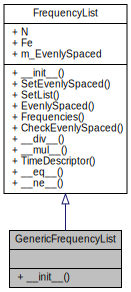
\includegraphics[width=203pt]{classSignalIntegrity_1_1FrequencyDomain_1_1FrequencyList_1_1GenericFrequencyList__coll__graph}
\end{center}
\end{figure}
\subsection*{Public Member Functions}
\begin{DoxyCompactItemize}
\item 
def \hyperlink{classSignalIntegrity_1_1FrequencyDomain_1_1FrequencyList_1_1GenericFrequencyList_a9a74e46546d1e8002152b5d0e79786c4}{\+\_\+\+\_\+init\+\_\+\+\_\+} (self, fl)
\begin{DoxyCompactList}\small\item\em Constructor. \end{DoxyCompactList}\end{DoxyCompactItemize}
\subsection*{Additional Inherited Members}


\subsection{Detailed Description}
A generic list of frequencies assumed to be not evenly spaced. 



Definition at line 219 of file Frequency\+List.\+py.



\subsection{Constructor \& Destructor Documentation}
\mbox{\Hypertarget{classSignalIntegrity_1_1FrequencyDomain_1_1FrequencyList_1_1GenericFrequencyList_a9a74e46546d1e8002152b5d0e79786c4}\label{classSignalIntegrity_1_1FrequencyDomain_1_1FrequencyList_1_1GenericFrequencyList_a9a74e46546d1e8002152b5d0e79786c4}} 
\index{Signal\+Integrity\+::\+Frequency\+Domain\+::\+Frequency\+List\+::\+Generic\+Frequency\+List@{Signal\+Integrity\+::\+Frequency\+Domain\+::\+Frequency\+List\+::\+Generic\+Frequency\+List}!\+\_\+\+\_\+init\+\_\+\+\_\+@{\+\_\+\+\_\+init\+\_\+\+\_\+}}
\index{\+\_\+\+\_\+init\+\_\+\+\_\+@{\+\_\+\+\_\+init\+\_\+\+\_\+}!Signal\+Integrity\+::\+Frequency\+Domain\+::\+Frequency\+List\+::\+Generic\+Frequency\+List@{Signal\+Integrity\+::\+Frequency\+Domain\+::\+Frequency\+List\+::\+Generic\+Frequency\+List}}
\subsubsection{\texorpdfstring{\+\_\+\+\_\+init\+\_\+\+\_\+()}{\_\_init\_\_()}}
{\footnotesize\ttfamily def \+\_\+\+\_\+init\+\_\+\+\_\+ (\begin{DoxyParamCaption}\item[{}]{self,  }\item[{}]{fl }\end{DoxyParamCaption})}



Constructor. 


\begin{DoxyParams}{Parameters}
{\em fl} & list of frequencies. \\
\hline
\end{DoxyParams}
\begin{DoxyReturn}{Returns}
self. 
\end{DoxyReturn}
\begin{DoxyRemark}{Remarks}
Initializes the frequency list with a list of frequencies.
\end{DoxyRemark}
This will set the List to the list provided, N to the length -\/1, and Fe to the frequency of the last element in the list. It will set m\+\_\+\+Evenly\+Spaced False.

\begin{DoxyNote}{Note}
although this initializer is meant to take a list of frequencies, it will also take an instance of class \hyperlink{classSignalIntegrity_1_1FrequencyDomain_1_1FrequencyList_1_1FrequencyList}{Frequency\+List}, as it mimics this list behavior. In this case, it will install it as if the \hyperlink{classSignalIntegrity_1_1FrequencyDomain_1_1FrequencyList_1_1FrequencyList}{Frequency\+List} instance was simply a list of frequencies. 
\end{DoxyNote}


Definition at line 234 of file Frequency\+List.\+py.



The documentation for this class was generated from the following file\+:\begin{DoxyCompactItemize}
\item 
Py\+S\+I/\+Signal\+Integrity/\+Frequency\+Domain/Frequency\+List.\+py\end{DoxyCompactItemize}

\hypertarget{classSignalIntegrity_1_1ImpedanceProfile_1_1ImpedanceProfileWaveform_1_1ImpedanceProfileWaveform}{}\section{Impedance\+Profile\+Waveform Class Reference}
\label{classSignalIntegrity_1_1ImpedanceProfile_1_1ImpedanceProfileWaveform_1_1ImpedanceProfileWaveform}\index{Impedance\+Profile\+Waveform@{Impedance\+Profile\+Waveform}}


Computes the impedance profile waveform from a set of s-\/parameters using the port specified.  




Inheritance diagram for Impedance\+Profile\+Waveform\+:
\nopagebreak
\begin{figure}[H]
\begin{center}
\leavevmode
\includegraphics[width=217pt]{classSignalIntegrity_1_1ImpedanceProfile_1_1ImpedanceProfileWaveform_1_1ImpedanceProfileWaveform__inherit__graph}
\end{center}
\end{figure}


Collaboration diagram for Impedance\+Profile\+Waveform\+:
\nopagebreak
\begin{figure}[H]
\begin{center}
\leavevmode
\includegraphics[width=217pt]{classSignalIntegrity_1_1ImpedanceProfile_1_1ImpedanceProfileWaveform_1_1ImpedanceProfileWaveform__coll__graph}
\end{center}
\end{figure}
\subsection*{Public Member Functions}
\begin{DoxyCompactItemize}
\item 
def \hyperlink{classSignalIntegrity_1_1ImpedanceProfile_1_1ImpedanceProfileWaveform_1_1ImpedanceProfileWaveform_a44c18ce4afb30f11f4cdb07bc0f0c6be}{\+\_\+\+\_\+init\+\_\+\+\_\+} (self, sp, port=1, method=\textquotesingle{}exact\textquotesingle{}, align=\textquotesingle{}middle\textquotesingle{}, include\+PortZ=True, adjust\+For\+Delay=True)
\begin{DoxyCompactList}\small\item\em Constructor. \end{DoxyCompactList}\end{DoxyCompactItemize}


\subsection{Detailed Description}
Computes the impedance profile waveform from a set of s-\/parameters using the port specified. 

method is \textquotesingle{}exact\textquotesingle{},\textquotesingle{}estimated\textquotesingle{} or \textquotesingle{}approximate\textquotesingle{} \textquotesingle{}exact\textquotesingle{} specifies to use the D\+FT method to deembed sections of impedance found at an interface. This method is exact in simulation. \textquotesingle{}estimated\textquotesingle{} and \textquotesingle{}approximate\textquotesingle{} both use the step response of the system computed from the s-\/parameters. \textquotesingle{}estimated\textquotesingle{} calculates the Z exactly, assuming the step response contains rho (the reflection coefficient), which is an estimate because rho is polluted by multiple reflections. \textquotesingle{}approximate\textquotesingle{} calculates Z using a simple offset and scaling like would be employed when viewing a T\+DR waveform. There is no reason to use \textquotesingle{}approximate\textquotesingle{} -\/ except for educational purposes. \textquotesingle{}exact\textquotesingle{} can be quite unstable. \textquotesingle{}Estimated\textquotesingle{} is actually usually the best method.

align is either \textquotesingle{}middle\textquotesingle{} or \textquotesingle{}interface\textquotesingle{} \textquotesingle{}middle\textquotesingle{} means that the impedance for each point produced is at the corresponding time representing the the middle of a transmission line section. \textquotesingle{}interface\textquotesingle{} means that the time of the impedance is the time of the left edge of a transmission line with the corresponding impedance.

include\+PortZ is set to True if you want the first point to be the impedance of the port used to take the measurement. 

Definition at line 48 of file Impedance\+Profile\+Waveform.\+py.



\subsection{Constructor \& Destructor Documentation}
\mbox{\Hypertarget{classSignalIntegrity_1_1ImpedanceProfile_1_1ImpedanceProfileWaveform_1_1ImpedanceProfileWaveform_a44c18ce4afb30f11f4cdb07bc0f0c6be}\label{classSignalIntegrity_1_1ImpedanceProfile_1_1ImpedanceProfileWaveform_1_1ImpedanceProfileWaveform_a44c18ce4afb30f11f4cdb07bc0f0c6be}} 
\index{Signal\+Integrity\+::\+Impedance\+Profile\+::\+Impedance\+Profile\+Waveform\+::\+Impedance\+Profile\+Waveform@{Signal\+Integrity\+::\+Impedance\+Profile\+::\+Impedance\+Profile\+Waveform\+::\+Impedance\+Profile\+Waveform}!\+\_\+\+\_\+init\+\_\+\+\_\+@{\+\_\+\+\_\+init\+\_\+\+\_\+}}
\index{\+\_\+\+\_\+init\+\_\+\+\_\+@{\+\_\+\+\_\+init\+\_\+\+\_\+}!Signal\+Integrity\+::\+Impedance\+Profile\+::\+Impedance\+Profile\+Waveform\+::\+Impedance\+Profile\+Waveform@{Signal\+Integrity\+::\+Impedance\+Profile\+::\+Impedance\+Profile\+Waveform\+::\+Impedance\+Profile\+Waveform}}
\subsubsection{\texorpdfstring{\+\_\+\+\_\+init\+\_\+\+\_\+()}{\_\_init\_\_()}}
{\footnotesize\ttfamily def \+\_\+\+\_\+init\+\_\+\+\_\+ (\begin{DoxyParamCaption}\item[{}]{self,  }\item[{}]{sp,  }\item[{}]{port = {\ttfamily 1},  }\item[{}]{method = {\ttfamily \textquotesingle{}exact\textquotesingle{}},  }\item[{}]{align = {\ttfamily \textquotesingle{}middle\textquotesingle{}},  }\item[{}]{include\+PortZ = {\ttfamily True},  }\item[{}]{adjust\+For\+Delay = {\ttfamily True} }\end{DoxyParamCaption})}



Constructor. 


\begin{DoxyParams}{Parameters}
{\em sp} & instance of class \hyperlink{namespaceSignalIntegrity_1_1SParameters}{S\+Parameters} of the device \\
\hline
{\em port} & (optional) integer 1 based port number (defaults to port 1) \\
\hline
{\em method} & (optional) string method for computation (defaults to \textquotesingle{}exact\textquotesingle{}) \\
\hline
{\em align} & (optional) string alignment of impedancance in waveform (defaults to \textquotesingle{}middle\textquotesingle{}) \\
\hline
{\em include\+PortZ} & (optional) boolean whether to put the port reference impedance as the first point. (defaults to True) \\
\hline
{\em adjust\+For\+Delay(optional)} & boolean whether to adjust for the delay in the impulse response (defaults to True) \\
\hline
\end{DoxyParams}
\begin{DoxyRemark}{Remarks}
computation methods include\+: \textquotesingle{}exact\textquotesingle{} (default) -\/ calculates using reflection coefficient of first point computed from D\+FT and deembedding. (this method takes longer and can diverge due to buildup of numerical inaccuracies.) \textquotesingle{}estimated\textquotesingle{} -\/ calculates the reflection coefficients directly from the step response. \textquotesingle{}approximate\textquotesingle{} -\/ calculates the reflection coefficients from the step response using an approximation. 

alignment methods include\+: \textquotesingle{}middle\textquotesingle{} (default) -\/ shows the impedance in the middle of the sample period distance along the line. \textquotesingle{}front\textquotesingle{} -\/ shows the impedance measured at the front of the line. 
\end{DoxyRemark}


Definition at line 69 of file Impedance\+Profile\+Waveform.\+py.



The documentation for this class was generated from the following file\+:\begin{DoxyCompactItemize}
\item 
Py\+S\+I/\+Signal\+Integrity/\+Impedance\+Profile/Impedance\+Profile\+Waveform.\+py\end{DoxyCompactItemize}

\hypertarget{classSignalIntegrity_1_1TimeDomain_1_1Waveform_1_1ImpulseResponse_1_1ImpulseResponse}{}\section{Impulse\+Response Class Reference}
\label{classSignalIntegrity_1_1TimeDomain_1_1Waveform_1_1ImpulseResponse_1_1ImpulseResponse}\index{Impulse\+Response@{Impulse\+Response}}


impulse response of a filter as a waveform  




Inheritance diagram for Impulse\+Response\+:
\nopagebreak
\begin{figure}[H]
\begin{center}
\leavevmode
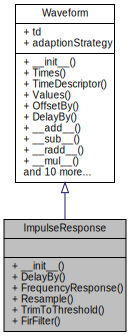
\includegraphics[width=202pt]{classSignalIntegrity_1_1TimeDomain_1_1Waveform_1_1ImpulseResponse_1_1ImpulseResponse__inherit__graph}
\end{center}
\end{figure}


Collaboration diagram for Impulse\+Response\+:
\nopagebreak
\begin{figure}[H]
\begin{center}
\leavevmode
\includegraphics[width=202pt]{classSignalIntegrity_1_1TimeDomain_1_1Waveform_1_1ImpulseResponse_1_1ImpulseResponse__coll__graph}
\end{center}
\end{figure}
\subsection*{Public Member Functions}
\begin{DoxyCompactItemize}
\item 
def \hyperlink{classSignalIntegrity_1_1TimeDomain_1_1Waveform_1_1ImpulseResponse_1_1ImpulseResponse_ade7e2b05916c8bb56f58333b3fca239d}{\+\_\+\+\_\+init\+\_\+\+\_\+} (self, t=None, td=None)
\begin{DoxyCompactList}\small\item\em constructor \end{DoxyCompactList}\item 
def \hyperlink{classSignalIntegrity_1_1TimeDomain_1_1Waveform_1_1ImpulseResponse_1_1ImpulseResponse_adc875e86caadbd6201fd6a3528526cad}{Delay\+By} (self, d)
\begin{DoxyCompactList}\small\item\em delays the impulse response \end{DoxyCompactList}\item 
def \hyperlink{classSignalIntegrity_1_1TimeDomain_1_1Waveform_1_1ImpulseResponse_1_1ImpulseResponse_a8a375a8188c5b58fa6f933db5737ddd1}{Frequency\+Response} (self, fd=None, adjust\+Length=True)
\begin{DoxyCompactList}\small\item\em produces the frequency response \end{DoxyCompactList}\item 
def \hyperlink{classSignalIntegrity_1_1TimeDomain_1_1Waveform_1_1ImpulseResponse_1_1ImpulseResponse_adc3851330110033606ca742a0025ae1a}{Resample} (self, td)
\begin{DoxyCompactList}\small\item\em resamples the impulse response to a specified time descriptor \end{DoxyCompactList}\item 
def \hyperlink{classSignalIntegrity_1_1TimeDomain_1_1Waveform_1_1ImpulseResponse_1_1ImpulseResponse_ac9668c22e21b9fcbfb1163ba5c2f9577}{Trim\+To\+Threshold} (self, threshold)
\begin{DoxyCompactList}\small\item\em truncates an impulse response, keeping only the values above or equal to specified threshold. \end{DoxyCompactList}\item 
def \hyperlink{classSignalIntegrity_1_1TimeDomain_1_1Waveform_1_1ImpulseResponse_1_1ImpulseResponse_a42a5eeb1a372a3e4c8beb7aed8cc2e13}{Fir\+Filter} (self)
\begin{DoxyCompactList}\small\item\em F\+IR filter equivalent of impulse response for processing. \end{DoxyCompactList}\end{DoxyCompactItemize}


\subsection{Detailed Description}
impulse response of a filter as a waveform 

Definition at line 27 of file Impulse\+Response.\+py.



\subsection{Constructor \& Destructor Documentation}
\mbox{\Hypertarget{classSignalIntegrity_1_1TimeDomain_1_1Waveform_1_1ImpulseResponse_1_1ImpulseResponse_ade7e2b05916c8bb56f58333b3fca239d}\label{classSignalIntegrity_1_1TimeDomain_1_1Waveform_1_1ImpulseResponse_1_1ImpulseResponse_ade7e2b05916c8bb56f58333b3fca239d}} 
\index{Signal\+Integrity\+::\+Time\+Domain\+::\+Waveform\+::\+Impulse\+Response\+::\+Impulse\+Response@{Signal\+Integrity\+::\+Time\+Domain\+::\+Waveform\+::\+Impulse\+Response\+::\+Impulse\+Response}!\+\_\+\+\_\+init\+\_\+\+\_\+@{\+\_\+\+\_\+init\+\_\+\+\_\+}}
\index{\+\_\+\+\_\+init\+\_\+\+\_\+@{\+\_\+\+\_\+init\+\_\+\+\_\+}!Signal\+Integrity\+::\+Time\+Domain\+::\+Waveform\+::\+Impulse\+Response\+::\+Impulse\+Response@{Signal\+Integrity\+::\+Time\+Domain\+::\+Waveform\+::\+Impulse\+Response\+::\+Impulse\+Response}}
\subsubsection{\texorpdfstring{\+\_\+\+\_\+init\+\_\+\+\_\+()}{\_\_init\_\_()}}
{\footnotesize\ttfamily def \+\_\+\+\_\+init\+\_\+\+\_\+ (\begin{DoxyParamCaption}\item[{}]{self,  }\item[{}]{t = {\ttfamily None},  }\item[{}]{td = {\ttfamily None} }\end{DoxyParamCaption})}



constructor 


\begin{DoxyParams}{Parameters}
{\em t} & instance of class \hyperlink{namespaceSignalIntegrity_1_1TimeDomain_1_1Waveform_1_1TimeDescriptor}{Time\+Descriptor} describing time-\/axis of impulse response \\
\hline
{\em td} & list of float representing time-\/domain values \\
\hline
\end{DoxyParams}
\begin{DoxyRemark}{Remarks}
note that t can be an instance of waveform and td None which causes the impulse response to be instantiated dircectly from a waveform. 
\end{DoxyRemark}


Definition at line 35 of file Impulse\+Response.\+py.



\subsection{Member Function Documentation}
\mbox{\Hypertarget{classSignalIntegrity_1_1TimeDomain_1_1Waveform_1_1ImpulseResponse_1_1ImpulseResponse_adc875e86caadbd6201fd6a3528526cad}\label{classSignalIntegrity_1_1TimeDomain_1_1Waveform_1_1ImpulseResponse_1_1ImpulseResponse_adc875e86caadbd6201fd6a3528526cad}} 
\index{Signal\+Integrity\+::\+Time\+Domain\+::\+Waveform\+::\+Impulse\+Response\+::\+Impulse\+Response@{Signal\+Integrity\+::\+Time\+Domain\+::\+Waveform\+::\+Impulse\+Response\+::\+Impulse\+Response}!Delay\+By@{Delay\+By}}
\index{Delay\+By@{Delay\+By}!Signal\+Integrity\+::\+Time\+Domain\+::\+Waveform\+::\+Impulse\+Response\+::\+Impulse\+Response@{Signal\+Integrity\+::\+Time\+Domain\+::\+Waveform\+::\+Impulse\+Response\+::\+Impulse\+Response}}
\subsubsection{\texorpdfstring{Delay\+By()}{DelayBy()}}
{\footnotesize\ttfamily def Delay\+By (\begin{DoxyParamCaption}\item[{}]{self,  }\item[{}]{d }\end{DoxyParamCaption})}



delays the impulse response 

delays the impulse response by modifying the time-\/axis under the response.


\begin{DoxyParams}{Parameters}
{\em d} & float time to delay the response by. \\
\hline
\end{DoxyParams}


Definition at line 47 of file Impulse\+Response.\+py.

\mbox{\Hypertarget{classSignalIntegrity_1_1TimeDomain_1_1Waveform_1_1ImpulseResponse_1_1ImpulseResponse_a42a5eeb1a372a3e4c8beb7aed8cc2e13}\label{classSignalIntegrity_1_1TimeDomain_1_1Waveform_1_1ImpulseResponse_1_1ImpulseResponse_a42a5eeb1a372a3e4c8beb7aed8cc2e13}} 
\index{Signal\+Integrity\+::\+Time\+Domain\+::\+Waveform\+::\+Impulse\+Response\+::\+Impulse\+Response@{Signal\+Integrity\+::\+Time\+Domain\+::\+Waveform\+::\+Impulse\+Response\+::\+Impulse\+Response}!Fir\+Filter@{Fir\+Filter}}
\index{Fir\+Filter@{Fir\+Filter}!Signal\+Integrity\+::\+Time\+Domain\+::\+Waveform\+::\+Impulse\+Response\+::\+Impulse\+Response@{Signal\+Integrity\+::\+Time\+Domain\+::\+Waveform\+::\+Impulse\+Response\+::\+Impulse\+Response}}
\subsubsection{\texorpdfstring{Fir\+Filter()}{FirFilter()}}
{\footnotesize\ttfamily def \hyperlink{classSignalIntegrity_1_1TimeDomain_1_1Filters_1_1FirFilter_1_1FirFilter}{Fir\+Filter} (\begin{DoxyParamCaption}\item[{}]{self }\end{DoxyParamCaption})}



F\+IR filter equivalent of impulse response for processing. 

\begin{DoxyReturn}{Returns}
an instance of class Fir\+Filter that can be convolved with a waveform 
\end{DoxyReturn}


Definition at line 219 of file Impulse\+Response.\+py.

\mbox{\Hypertarget{classSignalIntegrity_1_1TimeDomain_1_1Waveform_1_1ImpulseResponse_1_1ImpulseResponse_a8a375a8188c5b58fa6f933db5737ddd1}\label{classSignalIntegrity_1_1TimeDomain_1_1Waveform_1_1ImpulseResponse_1_1ImpulseResponse_a8a375a8188c5b58fa6f933db5737ddd1}} 
\index{Signal\+Integrity\+::\+Time\+Domain\+::\+Waveform\+::\+Impulse\+Response\+::\+Impulse\+Response@{Signal\+Integrity\+::\+Time\+Domain\+::\+Waveform\+::\+Impulse\+Response\+::\+Impulse\+Response}!Frequency\+Response@{Frequency\+Response}}
\index{Frequency\+Response@{Frequency\+Response}!Signal\+Integrity\+::\+Time\+Domain\+::\+Waveform\+::\+Impulse\+Response\+::\+Impulse\+Response@{Signal\+Integrity\+::\+Time\+Domain\+::\+Waveform\+::\+Impulse\+Response\+::\+Impulse\+Response}}
\subsubsection{\texorpdfstring{Frequency\+Response()}{FrequencyResponse()}}
{\footnotesize\ttfamily def Frequency\+Response (\begin{DoxyParamCaption}\item[{}]{self,  }\item[{}]{fd = {\ttfamily None},  }\item[{}]{adjust\+Length = {\ttfamily True} }\end{DoxyParamCaption})}



produces the frequency response 

impulse responses and frequency responses are equivalent and can be converted back and forth into each other. This method converts the impulse response to its corresponding frequency domain equivalent.

\begin{DoxyAttention}{Attention}
users of this function should only either supply the fd argument or not. Not supplying the argument provides the generic frequency response associated with this impulse response such that self.\+Frequency\+Response().Impulse\+Response() provides the same answer.
\end{DoxyAttention}
Supplying fd supplies the resulting frequency response resampled onto another frequency scale.


\begin{DoxyParams}{Parameters}
{\em fd} & (optional) instance of class Frequency\+Descriptor (defaults to None). \\
\hline
{\em adjust\+Length} & (optional) bool whether to adjust the length. (defaults to True).\\
\hline
\end{DoxyParams}
\begin{DoxyNote}{Note}
All impulse responses are evenly spaced

whether a frequency descriptor is specified and whether to adjust length determines all possibilities of what can happen\+:
\end{DoxyNote}
\tabulinesep=1mm
\begin{longtabu} spread 0pt [c]{*{3}{|X[-1]}|}
\hline
\rowcolor{\tableheadbgcolor}\PBS\centering \textbf{ fd }&\PBS\centering \textbf{ adjust\+Length }&\PBS\centering \textbf{ Generates\+:  }\\\cline{1-3}
\endfirsthead
\hline
\endfoot
\hline
\rowcolor{\tableheadbgcolor}\PBS\centering \textbf{ fd }&\PBS\centering \textbf{ adjust\+Length }&\PBS\centering \textbf{ Generates\+:  }\\\cline{1-3}
\endhead
\PBS\centering None &\PBS\centering False &\PBS\centering generic frequency response \\\cline{1-3}
\PBS\centering None &\PBS\centering True &\PBS\centering frequency response with length adjusted \\\cline{1-3}
\PBS\centering provided &\PBS\centering don\textquotesingle{}t care &\PBS\centering C\+ZT resamples to fd (adjusts length) \\\cline{1-3}
\end{longtabu}
The frequency descriptor, if provided, provides the frequency points to resample to, otherwise the frequency descriptor associated with the internal time descriptor inherent to the impulse response is used.

Length adjustment means that although the impulse response may start at time zero, or some other time, the assumption is that there are an equal number of points for negative and positve time and that time zero is in the center of these points.

This assumption for length adjustment is what allows an impulse response to be filled in with positive only times, but allow an equality to exist between all frequency responses and impulse responses.

Basically, the time adjustment can be seen as calculating the number of points before time zero and the number of points after time zero and calculating the total number of points in the waveform (for the purposes of frequency response calculation) as the max of these two numbers multiplied by two. 

Definition at line 92 of file Impulse\+Response.\+py.

\mbox{\Hypertarget{classSignalIntegrity_1_1TimeDomain_1_1Waveform_1_1ImpulseResponse_1_1ImpulseResponse_adc3851330110033606ca742a0025ae1a}\label{classSignalIntegrity_1_1TimeDomain_1_1Waveform_1_1ImpulseResponse_1_1ImpulseResponse_adc3851330110033606ca742a0025ae1a}} 
\index{Signal\+Integrity\+::\+Time\+Domain\+::\+Waveform\+::\+Impulse\+Response\+::\+Impulse\+Response@{Signal\+Integrity\+::\+Time\+Domain\+::\+Waveform\+::\+Impulse\+Response\+::\+Impulse\+Response}!Resample@{Resample}}
\index{Resample@{Resample}!Signal\+Integrity\+::\+Time\+Domain\+::\+Waveform\+::\+Impulse\+Response\+::\+Impulse\+Response@{Signal\+Integrity\+::\+Time\+Domain\+::\+Waveform\+::\+Impulse\+Response\+::\+Impulse\+Response}}
\subsubsection{\texorpdfstring{Resample()}{Resample()}}
{\footnotesize\ttfamily def Resample (\begin{DoxyParamCaption}\item[{}]{self,  }\item[{}]{td }\end{DoxyParamCaption})}



resamples the impulse response to a specified time descriptor 


\begin{DoxyParams}{Parameters}
{\em td} & instance of class \hyperlink{namespaceSignalIntegrity_1_1TimeDomain_1_1Waveform_1_1TimeDescriptor}{Time\+Descriptor} containing new time descriptor. \\
\hline
\end{DoxyParams}
\begin{DoxyReturn}{Returns}
an instance of class \hyperlink{classSignalIntegrity_1_1TimeDomain_1_1Waveform_1_1ImpulseResponse_1_1ImpulseResponse}{Impulse\+Response} containing impulse response with new time descriptor. 
\end{DoxyReturn}


Definition at line 168 of file Impulse\+Response.\+py.

\mbox{\Hypertarget{classSignalIntegrity_1_1TimeDomain_1_1Waveform_1_1ImpulseResponse_1_1ImpulseResponse_ac9668c22e21b9fcbfb1163ba5c2f9577}\label{classSignalIntegrity_1_1TimeDomain_1_1Waveform_1_1ImpulseResponse_1_1ImpulseResponse_ac9668c22e21b9fcbfb1163ba5c2f9577}} 
\index{Signal\+Integrity\+::\+Time\+Domain\+::\+Waveform\+::\+Impulse\+Response\+::\+Impulse\+Response@{Signal\+Integrity\+::\+Time\+Domain\+::\+Waveform\+::\+Impulse\+Response\+::\+Impulse\+Response}!Trim\+To\+Threshold@{Trim\+To\+Threshold}}
\index{Trim\+To\+Threshold@{Trim\+To\+Threshold}!Signal\+Integrity\+::\+Time\+Domain\+::\+Waveform\+::\+Impulse\+Response\+::\+Impulse\+Response@{Signal\+Integrity\+::\+Time\+Domain\+::\+Waveform\+::\+Impulse\+Response\+::\+Impulse\+Response}}
\subsubsection{\texorpdfstring{Trim\+To\+Threshold()}{TrimToThreshold()}}
{\footnotesize\ttfamily def Trim\+To\+Threshold (\begin{DoxyParamCaption}\item[{}]{self,  }\item[{}]{threshold }\end{DoxyParamCaption})}



truncates an impulse response, keeping only the values above or equal to specified threshold. 

This is useful for reducing computational complexity in processing.


\begin{DoxyParams}{Parameters}
{\em threshold} & float threshold to apply to the values in the waveform. \\
\hline
\end{DoxyParams}
\begin{DoxyAttention}{Attention}
the threshold specified is a fraction of the maximum absolute value of the values in the waveform. 
\end{DoxyAttention}
\begin{DoxyNote}{Note}
that absolute values are utilized in value/threshold comparison. 

the trimming is performed by finding the lowest and highest time value above or equal to the threshold -\/ all values between these times are retained. 
\end{DoxyNote}


Definition at line 183 of file Impulse\+Response.\+py.



The documentation for this class was generated from the following file\+:\begin{DoxyCompactItemize}
\item 
Py\+S\+I/\+Signal\+Integrity/\+Time\+Domain/\+Waveform/Impulse\+Response.\+py\end{DoxyCompactItemize}

\hypertarget{classSignalIntegrity_1_1TimeDomain_1_1Filters_1_1InterpolatorLinear_1_1InterpolatorFractionalDelayFilterLinear}{}\section{Interpolator\+Fractional\+Delay\+Filter\+Linear Class Reference}
\label{classSignalIntegrity_1_1TimeDomain_1_1Filters_1_1InterpolatorLinear_1_1InterpolatorFractionalDelayFilterLinear}\index{Interpolator\+Fractional\+Delay\+Filter\+Linear@{Interpolator\+Fractional\+Delay\+Filter\+Linear}}


combination linear fractional delay and interpolating filter  




Inheritance diagram for Interpolator\+Fractional\+Delay\+Filter\+Linear\+:
\nopagebreak
\begin{figure}[H]
\begin{center}
\leavevmode
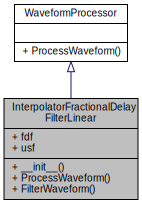
\includegraphics[width=214pt]{classSignalIntegrity_1_1TimeDomain_1_1Filters_1_1InterpolatorLinear_1_1InterpolatorFractionalDelayFilterLinear__inherit__graph}
\end{center}
\end{figure}


Collaboration diagram for Interpolator\+Fractional\+Delay\+Filter\+Linear\+:
\nopagebreak
\begin{figure}[H]
\begin{center}
\leavevmode
\includegraphics[width=214pt]{classSignalIntegrity_1_1TimeDomain_1_1Filters_1_1InterpolatorLinear_1_1InterpolatorFractionalDelayFilterLinear__coll__graph}
\end{center}
\end{figure}
\subsection*{Public Member Functions}
\begin{DoxyCompactItemize}
\item 
def \hyperlink{classSignalIntegrity_1_1TimeDomain_1_1Filters_1_1InterpolatorLinear_1_1InterpolatorFractionalDelayFilterLinear_a81150f52975e0ef244e215c5faf0291e}{\+\_\+\+\_\+init\+\_\+\+\_\+} (self, U, F, account\+For\+Delay=True)
\begin{DoxyCompactList}\small\item\em Constructor. \end{DoxyCompactList}\item 
def \hyperlink{classSignalIntegrity_1_1TimeDomain_1_1Filters_1_1InterpolatorLinear_1_1InterpolatorFractionalDelayFilterLinear_ae09bec195c9cb1d5819e73b7be169b11}{Process\+Waveform} (self, wf)
\begin{DoxyCompactList}\small\item\em process waveform \end{DoxyCompactList}\item 
def \hyperlink{classSignalIntegrity_1_1TimeDomain_1_1Filters_1_1InterpolatorLinear_1_1InterpolatorFractionalDelayFilterLinear_a84e73c18250ca4a61482f94ad61e735b}{Filter\+Waveform} (self, wf)
\begin{DoxyCompactList}\small\item\em overloads base class Filter\+Waveform \end{DoxyCompactList}\end{DoxyCompactItemize}


\subsection{Detailed Description}
combination linear fractional delay and interpolating filter 

Definition at line 85 of file Interpolator\+Linear.\+py.



\subsection{Constructor \& Destructor Documentation}
\mbox{\Hypertarget{classSignalIntegrity_1_1TimeDomain_1_1Filters_1_1InterpolatorLinear_1_1InterpolatorFractionalDelayFilterLinear_a81150f52975e0ef244e215c5faf0291e}\label{classSignalIntegrity_1_1TimeDomain_1_1Filters_1_1InterpolatorLinear_1_1InterpolatorFractionalDelayFilterLinear_a81150f52975e0ef244e215c5faf0291e}} 
\index{Signal\+Integrity\+::\+Time\+Domain\+::\+Filters\+::\+Interpolator\+Linear\+::\+Interpolator\+Fractional\+Delay\+Filter\+Linear@{Signal\+Integrity\+::\+Time\+Domain\+::\+Filters\+::\+Interpolator\+Linear\+::\+Interpolator\+Fractional\+Delay\+Filter\+Linear}!\+\_\+\+\_\+init\+\_\+\+\_\+@{\+\_\+\+\_\+init\+\_\+\+\_\+}}
\index{\+\_\+\+\_\+init\+\_\+\+\_\+@{\+\_\+\+\_\+init\+\_\+\+\_\+}!Signal\+Integrity\+::\+Time\+Domain\+::\+Filters\+::\+Interpolator\+Linear\+::\+Interpolator\+Fractional\+Delay\+Filter\+Linear@{Signal\+Integrity\+::\+Time\+Domain\+::\+Filters\+::\+Interpolator\+Linear\+::\+Interpolator\+Fractional\+Delay\+Filter\+Linear}}
\subsubsection{\texorpdfstring{\+\_\+\+\_\+init\+\_\+\+\_\+()}{\_\_init\_\_()}}
{\footnotesize\ttfamily def \+\_\+\+\_\+init\+\_\+\+\_\+ (\begin{DoxyParamCaption}\item[{}]{self,  }\item[{}]{U,  }\item[{}]{F,  }\item[{}]{account\+For\+Delay = {\ttfamily True} }\end{DoxyParamCaption})}



Constructor. 


\begin{DoxyParams}{Parameters}
{\em U} & integer upsample factor of the filter. \\
\hline
{\em F} & float amount of delay to apply. The delay is in samples of the input waveform. \\
\hline
{\em account\+For\+Delay} & (optional) boolean whether to account for the delay \\
\hline
\end{DoxyParams}
\begin{DoxyRemark}{Remarks}
if account\+For\+Delay, then the filter provides a sample phase adjustment, meaning that there is no actual delay applied to the waveform, but the time axis under the waveform is shifted. This is the usual way to apply this filter and is used to adapt waveforms on different time axes to each other.~\newline
 if not account\+For\+Delay, then the filter actually delays waveforms by the delay specified. 
\end{DoxyRemark}


Definition at line 99 of file Interpolator\+Linear.\+py.



\subsection{Member Function Documentation}
\mbox{\Hypertarget{classSignalIntegrity_1_1TimeDomain_1_1Filters_1_1InterpolatorLinear_1_1InterpolatorFractionalDelayFilterLinear_a84e73c18250ca4a61482f94ad61e735b}\label{classSignalIntegrity_1_1TimeDomain_1_1Filters_1_1InterpolatorLinear_1_1InterpolatorFractionalDelayFilterLinear_a84e73c18250ca4a61482f94ad61e735b}} 
\index{Signal\+Integrity\+::\+Time\+Domain\+::\+Filters\+::\+Interpolator\+Linear\+::\+Interpolator\+Fractional\+Delay\+Filter\+Linear@{Signal\+Integrity\+::\+Time\+Domain\+::\+Filters\+::\+Interpolator\+Linear\+::\+Interpolator\+Fractional\+Delay\+Filter\+Linear}!Filter\+Waveform@{Filter\+Waveform}}
\index{Filter\+Waveform@{Filter\+Waveform}!Signal\+Integrity\+::\+Time\+Domain\+::\+Filters\+::\+Interpolator\+Linear\+::\+Interpolator\+Fractional\+Delay\+Filter\+Linear@{Signal\+Integrity\+::\+Time\+Domain\+::\+Filters\+::\+Interpolator\+Linear\+::\+Interpolator\+Fractional\+Delay\+Filter\+Linear}}
\subsubsection{\texorpdfstring{Filter\+Waveform()}{FilterWaveform()}}
{\footnotesize\ttfamily def Filter\+Waveform (\begin{DoxyParamCaption}\item[{}]{self,  }\item[{}]{wf }\end{DoxyParamCaption})}



overloads base class Filter\+Waveform 


\begin{DoxyParams}{Parameters}
{\em wf} & instance of class \hyperlink{namespaceSignalIntegrity_1_1TimeDomain_1_1Waveform}{Waveform} of waveform to process \\
\hline
\end{DoxyParams}
\begin{DoxyReturn}{Returns}
instance of class \hyperlink{namespaceSignalIntegrity_1_1TimeDomain_1_1Waveform}{Waveform} of wf upsampled and fractionally delayed 
\end{DoxyReturn}


Definition at line 119 of file Interpolator\+Linear.\+py.

\mbox{\Hypertarget{classSignalIntegrity_1_1TimeDomain_1_1Filters_1_1InterpolatorLinear_1_1InterpolatorFractionalDelayFilterLinear_ae09bec195c9cb1d5819e73b7be169b11}\label{classSignalIntegrity_1_1TimeDomain_1_1Filters_1_1InterpolatorLinear_1_1InterpolatorFractionalDelayFilterLinear_ae09bec195c9cb1d5819e73b7be169b11}} 
\index{Signal\+Integrity\+::\+Time\+Domain\+::\+Filters\+::\+Interpolator\+Linear\+::\+Interpolator\+Fractional\+Delay\+Filter\+Linear@{Signal\+Integrity\+::\+Time\+Domain\+::\+Filters\+::\+Interpolator\+Linear\+::\+Interpolator\+Fractional\+Delay\+Filter\+Linear}!Process\+Waveform@{Process\+Waveform}}
\index{Process\+Waveform@{Process\+Waveform}!Signal\+Integrity\+::\+Time\+Domain\+::\+Filters\+::\+Interpolator\+Linear\+::\+Interpolator\+Fractional\+Delay\+Filter\+Linear@{Signal\+Integrity\+::\+Time\+Domain\+::\+Filters\+::\+Interpolator\+Linear\+::\+Interpolator\+Fractional\+Delay\+Filter\+Linear}}
\subsubsection{\texorpdfstring{Process\+Waveform()}{ProcessWaveform()}}
{\footnotesize\ttfamily def Process\+Waveform (\begin{DoxyParamCaption}\item[{}]{self,  }\item[{}]{wf }\end{DoxyParamCaption})}



process waveform 

waveforms are processed with both an interpolation and fractional delay filter.


\begin{DoxyParams}{Parameters}
{\em wf} & instance of class \hyperlink{namespaceSignalIntegrity_1_1TimeDomain_1_1Waveform}{Waveform} to filter \\
\hline
\end{DoxyParams}
\begin{DoxyReturn}{Returns}
instance of class \hyperlink{namespaceSignalIntegrity_1_1TimeDomain_1_1Waveform}{Waveform} of wf upsampled and fractionally delayed
\end{DoxyReturn}
\begin{DoxySeeAlso}{See also}
\hyperlink{classSignalIntegrity_1_1TimeDomain_1_1Filters_1_1InterpolatorLinear_1_1InterpolatorFractionalDelayFilterLinear_a84e73c18250ca4a61482f94ad61e735b}{Filter\+Waveform} 
\end{DoxySeeAlso}


Definition at line 112 of file Interpolator\+Linear.\+py.



The documentation for this class was generated from the following file\+:\begin{DoxyCompactItemize}
\item 
Py\+S\+I/\+Signal\+Integrity/\+Time\+Domain/\+Filters/Interpolator\+Linear.\+py\end{DoxyCompactItemize}

\input{classSignalIntegrity_1_1TimeDomain_1_1Filters_1_1InterpolatorSinX_1_1InterpolatorFractionalDelayFilterSinX}
\hypertarget{classSignalIntegrity_1_1TimeDomain_1_1Filters_1_1InterpolatorLinear_1_1InterpolatorLinear}{}\section{Interpolator\+Linear Class Reference}
\label{classSignalIntegrity_1_1TimeDomain_1_1Filters_1_1InterpolatorLinear_1_1InterpolatorLinear}\index{Interpolator\+Linear@{Interpolator\+Linear}}


linear interpolating filter  




Inheritance diagram for Interpolator\+Linear\+:\nopagebreak
\begin{figure}[H]
\begin{center}
\leavevmode
\includegraphics[width=193pt]{classSignalIntegrity_1_1TimeDomain_1_1Filters_1_1InterpolatorLinear_1_1InterpolatorLinear__inherit__graph}
\end{center}
\end{figure}


Collaboration diagram for Interpolator\+Linear\+:\nopagebreak
\begin{figure}[H]
\begin{center}
\leavevmode
\includegraphics[width=193pt]{classSignalIntegrity_1_1TimeDomain_1_1Filters_1_1InterpolatorLinear_1_1InterpolatorLinear__coll__graph}
\end{center}
\end{figure}
\subsection*{Public Member Functions}
\begin{DoxyCompactItemize}
\item 
def \hyperlink{classSignalIntegrity_1_1TimeDomain_1_1Filters_1_1InterpolatorLinear_1_1InterpolatorLinear_abff7619574bd23d3249b999fcc5bc87b}{\+\_\+\+\_\+init\+\_\+\+\_\+} (self, U)
\begin{DoxyCompactList}\small\item\em Constructor. \end{DoxyCompactList}\item 
def \hyperlink{classSignalIntegrity_1_1TimeDomain_1_1Filters_1_1InterpolatorLinear_1_1InterpolatorLinear_a84e73c18250ca4a61482f94ad61e735b}{Filter\+Waveform} (self, wf)
\begin{DoxyCompactList}\small\item\em overloads base class Filter\+Waveform \end{DoxyCompactList}\end{DoxyCompactItemize}


\subsection{Detailed Description}
linear interpolating filter 

Definition at line 41 of file Interpolator\+Linear.\+py.



\subsection{Constructor \& Destructor Documentation}
\mbox{\Hypertarget{classSignalIntegrity_1_1TimeDomain_1_1Filters_1_1InterpolatorLinear_1_1InterpolatorLinear_abff7619574bd23d3249b999fcc5bc87b}\label{classSignalIntegrity_1_1TimeDomain_1_1Filters_1_1InterpolatorLinear_1_1InterpolatorLinear_abff7619574bd23d3249b999fcc5bc87b}} 
\index{Signal\+Integrity\+::\+Time\+Domain\+::\+Filters\+::\+Interpolator\+Linear\+::\+Interpolator\+Linear@{Signal\+Integrity\+::\+Time\+Domain\+::\+Filters\+::\+Interpolator\+Linear\+::\+Interpolator\+Linear}!\+\_\+\+\_\+init\+\_\+\+\_\+@{\+\_\+\+\_\+init\+\_\+\+\_\+}}
\index{\+\_\+\+\_\+init\+\_\+\+\_\+@{\+\_\+\+\_\+init\+\_\+\+\_\+}!Signal\+Integrity\+::\+Time\+Domain\+::\+Filters\+::\+Interpolator\+Linear\+::\+Interpolator\+Linear@{Signal\+Integrity\+::\+Time\+Domain\+::\+Filters\+::\+Interpolator\+Linear\+::\+Interpolator\+Linear}}
\subsubsection{\texorpdfstring{\+\_\+\+\_\+init\+\_\+\+\_\+()}{\_\_init\_\_()}}
{\footnotesize\ttfamily def \+\_\+\+\_\+init\+\_\+\+\_\+ (\begin{DoxyParamCaption}\item[{}]{self,  }\item[{}]{U }\end{DoxyParamCaption})}



Constructor. 

applies a linear interpolating filter.


\begin{DoxyParams}{Parameters}
{\em U} & integer upsample factor of the filter. \\
\hline
\end{DoxyParams}


Definition at line 49 of file Interpolator\+Linear.\+py.



\subsection{Member Function Documentation}
\mbox{\Hypertarget{classSignalIntegrity_1_1TimeDomain_1_1Filters_1_1InterpolatorLinear_1_1InterpolatorLinear_a84e73c18250ca4a61482f94ad61e735b}\label{classSignalIntegrity_1_1TimeDomain_1_1Filters_1_1InterpolatorLinear_1_1InterpolatorLinear_a84e73c18250ca4a61482f94ad61e735b}} 
\index{Signal\+Integrity\+::\+Time\+Domain\+::\+Filters\+::\+Interpolator\+Linear\+::\+Interpolator\+Linear@{Signal\+Integrity\+::\+Time\+Domain\+::\+Filters\+::\+Interpolator\+Linear\+::\+Interpolator\+Linear}!Filter\+Waveform@{Filter\+Waveform}}
\index{Filter\+Waveform@{Filter\+Waveform}!Signal\+Integrity\+::\+Time\+Domain\+::\+Filters\+::\+Interpolator\+Linear\+::\+Interpolator\+Linear@{Signal\+Integrity\+::\+Time\+Domain\+::\+Filters\+::\+Interpolator\+Linear\+::\+Interpolator\+Linear}}
\subsubsection{\texorpdfstring{Filter\+Waveform()}{FilterWaveform()}}
{\footnotesize\ttfamily def Filter\+Waveform (\begin{DoxyParamCaption}\item[{}]{self,  }\item[{}]{wf }\end{DoxyParamCaption})}



overloads base class Filter\+Waveform 


\begin{DoxyParams}{Parameters}
{\em wf} & instance of class \hyperlink{namespaceSignalIntegrity_1_1TimeDomain_1_1Waveform}{Waveform} \\
\hline
\end{DoxyParams}
\begin{DoxyReturn}{Returns}
instance of class \hyperlink{namespaceSignalIntegrity_1_1TimeDomain_1_1Waveform}{Waveform} containing the upsampled, interpolated wf 
\end{DoxyReturn}
\begin{DoxyRemark}{Remarks}
This method first classically upsamples the waveform by inserting zeros between the samples and then passes the upsampled waveform through the linear interpolation filter. 
\end{DoxyRemark}


Definition at line 66 of file Interpolator\+Linear.\+py.



The documentation for this class was generated from the following file\+:\begin{DoxyCompactItemize}
\item 
Py\+S\+I/\+Signal\+Integrity/\+Time\+Domain/\+Filters/Interpolator\+Linear.\+py\end{DoxyCompactItemize}

\hypertarget{classSignalIntegrity_1_1TimeDomain_1_1Filters_1_1InterpolatorSinX_1_1InterpolatorSinX}{}\section{Interpolator\+SinX Class Reference}
\label{classSignalIntegrity_1_1TimeDomain_1_1Filters_1_1InterpolatorSinX_1_1InterpolatorSinX}\index{Interpolator\+SinX@{Interpolator\+SinX}}


sinx/x interpolating filter  




Inheritance diagram for Interpolator\+SinX\+:\nopagebreak
\begin{figure}[H]
\begin{center}
\leavevmode
\includegraphics[width=193pt]{classSignalIntegrity_1_1TimeDomain_1_1Filters_1_1InterpolatorSinX_1_1InterpolatorSinX__inherit__graph}
\end{center}
\end{figure}


Collaboration diagram for Interpolator\+SinX\+:\nopagebreak
\begin{figure}[H]
\begin{center}
\leavevmode
\includegraphics[width=193pt]{classSignalIntegrity_1_1TimeDomain_1_1Filters_1_1InterpolatorSinX_1_1InterpolatorSinX__coll__graph}
\end{center}
\end{figure}
\subsection*{Public Member Functions}
\begin{DoxyCompactItemize}
\item 
def \hyperlink{classSignalIntegrity_1_1TimeDomain_1_1Filters_1_1InterpolatorSinX_1_1InterpolatorSinX_abff7619574bd23d3249b999fcc5bc87b}{\+\_\+\+\_\+init\+\_\+\+\_\+} (self, U)
\begin{DoxyCompactList}\small\item\em Constructor. \end{DoxyCompactList}\item 
def \hyperlink{classSignalIntegrity_1_1TimeDomain_1_1Filters_1_1InterpolatorSinX_1_1InterpolatorSinX_a84e73c18250ca4a61482f94ad61e735b}{Filter\+Waveform} (self, wf)
\begin{DoxyCompactList}\small\item\em overloads base class Filter\+Waveform \end{DoxyCompactList}\end{DoxyCompactItemize}


\subsection{Detailed Description}
sinx/x interpolating filter 

Definition at line 68 of file Interpolator\+Sin\+X.\+py.



\subsection{Constructor \& Destructor Documentation}
\mbox{\Hypertarget{classSignalIntegrity_1_1TimeDomain_1_1Filters_1_1InterpolatorSinX_1_1InterpolatorSinX_abff7619574bd23d3249b999fcc5bc87b}\label{classSignalIntegrity_1_1TimeDomain_1_1Filters_1_1InterpolatorSinX_1_1InterpolatorSinX_abff7619574bd23d3249b999fcc5bc87b}} 
\index{Signal\+Integrity\+::\+Time\+Domain\+::\+Filters\+::\+Interpolator\+Sin\+X\+::\+Interpolator\+SinX@{Signal\+Integrity\+::\+Time\+Domain\+::\+Filters\+::\+Interpolator\+Sin\+X\+::\+Interpolator\+SinX}!\+\_\+\+\_\+init\+\_\+\+\_\+@{\+\_\+\+\_\+init\+\_\+\+\_\+}}
\index{\+\_\+\+\_\+init\+\_\+\+\_\+@{\+\_\+\+\_\+init\+\_\+\+\_\+}!Signal\+Integrity\+::\+Time\+Domain\+::\+Filters\+::\+Interpolator\+Sin\+X\+::\+Interpolator\+SinX@{Signal\+Integrity\+::\+Time\+Domain\+::\+Filters\+::\+Interpolator\+Sin\+X\+::\+Interpolator\+SinX}}
\subsubsection{\texorpdfstring{\+\_\+\+\_\+init\+\_\+\+\_\+()}{\_\_init\_\_()}}
{\footnotesize\ttfamily def \+\_\+\+\_\+init\+\_\+\+\_\+ (\begin{DoxyParamCaption}\item[{}]{self,  }\item[{}]{U }\end{DoxyParamCaption})}



Constructor. 

applies a sinx/x interpolating filter.


\begin{DoxyParams}{Parameters}
{\em U} & integer upsample factor of the filter. \\
\hline
\end{DoxyParams}


Definition at line 77 of file Interpolator\+Sin\+X.\+py.



\subsection{Member Function Documentation}
\mbox{\Hypertarget{classSignalIntegrity_1_1TimeDomain_1_1Filters_1_1InterpolatorSinX_1_1InterpolatorSinX_a84e73c18250ca4a61482f94ad61e735b}\label{classSignalIntegrity_1_1TimeDomain_1_1Filters_1_1InterpolatorSinX_1_1InterpolatorSinX_a84e73c18250ca4a61482f94ad61e735b}} 
\index{Signal\+Integrity\+::\+Time\+Domain\+::\+Filters\+::\+Interpolator\+Sin\+X\+::\+Interpolator\+SinX@{Signal\+Integrity\+::\+Time\+Domain\+::\+Filters\+::\+Interpolator\+Sin\+X\+::\+Interpolator\+SinX}!Filter\+Waveform@{Filter\+Waveform}}
\index{Filter\+Waveform@{Filter\+Waveform}!Signal\+Integrity\+::\+Time\+Domain\+::\+Filters\+::\+Interpolator\+Sin\+X\+::\+Interpolator\+SinX@{Signal\+Integrity\+::\+Time\+Domain\+::\+Filters\+::\+Interpolator\+Sin\+X\+::\+Interpolator\+SinX}}
\subsubsection{\texorpdfstring{Filter\+Waveform()}{FilterWaveform()}}
{\footnotesize\ttfamily def Filter\+Waveform (\begin{DoxyParamCaption}\item[{}]{self,  }\item[{}]{wf }\end{DoxyParamCaption})}



overloads base class Filter\+Waveform 


\begin{DoxyParams}{Parameters}
{\em wf} & instance of class \hyperlink{namespaceSignalIntegrity_1_1TimeDomain_1_1Waveform}{Waveform} \\
\hline
\end{DoxyParams}
\begin{DoxyReturn}{Returns}
instance of class \hyperlink{namespaceSignalIntegrity_1_1TimeDomain_1_1Waveform}{Waveform} containing the upsampled, interpolated wf 
\end{DoxyReturn}
\begin{DoxyRemark}{Remarks}
This method first classically upsamples the waveform by inserting zeros between the samples and then passes the upsampled waveform through the sinx/x interpolation filter. 
\end{DoxyRemark}


Definition at line 92 of file Interpolator\+Sin\+X.\+py.



The documentation for this class was generated from the following file\+:\begin{DoxyCompactItemize}
\item 
Py\+S\+I/\+Signal\+Integrity/\+Time\+Domain/\+Filters/Interpolator\+Sin\+X.\+py\end{DoxyCompactItemize}

\hypertarget{classSignalIntegrity_1_1Fit_1_1LevMar_1_1LevMar}{}\section{Lev\+Mar Class Reference}
\label{classSignalIntegrity_1_1Fit_1_1LevMar_1_1LevMar}\index{Lev\+Mar@{Lev\+Mar}}


Implements the Levenberg-\/\+Marquardt algorithm for non-\/linear fitting.  




Inheritance diagram for Lev\+Mar\+:
\nopagebreak
\begin{figure}[H]
\begin{center}
\leavevmode
\includegraphics[width=236pt]{classSignalIntegrity_1_1Fit_1_1LevMar_1_1LevMar__inherit__graph}
\end{center}
\end{figure}


Collaboration diagram for Lev\+Mar\+:
\nopagebreak
\begin{figure}[H]
\begin{center}
\leavevmode
\includegraphics[width=236pt]{classSignalIntegrity_1_1Fit_1_1LevMar_1_1LevMar__coll__graph}
\end{center}
\end{figure}
\subsection*{Public Member Functions}
\begin{DoxyCompactItemize}
\item 
def \hyperlink{classSignalIntegrity_1_1Fit_1_1LevMar_1_1LevMar_a5580a7fcf0bfd317a8f8c7c80eefdd69}{\+\_\+\+\_\+init\+\_\+\+\_\+} (self, callback=None)
\begin{DoxyCompactList}\small\item\em Constructor. \end{DoxyCompactList}\item 
def \hyperlink{classSignalIntegrity_1_1Fit_1_1LevMar_1_1LevMar_a4657ab652abd49c90e9541299fa5e9d8}{fF} (self, a)
\begin{DoxyCompactList}\small\item\em implements F(a) \end{DoxyCompactList}\item 
def \hyperlink{classSignalIntegrity_1_1Fit_1_1LevMar_1_1LevMar_a2cb2f2f3d90e9eff6180a5b6a5ffa5cc}{f\+Partial\+F\+Partiala} (self, a, m, Fa=None)
\begin{DoxyCompactList}\small\item\em partial derivative of F(a) with respect to a\mbox{[}m\mbox{]} \end{DoxyCompactList}\item 
def \hyperlink{classSignalIntegrity_1_1Fit_1_1LevMar_1_1LevMar_a5852efb9aab8530b863efac8008cd425}{fJ} (self, a, Fa=None)
\begin{DoxyCompactList}\small\item\em Calculates the Jacobian matrix. \end{DoxyCompactList}\item 
def \hyperlink{classSignalIntegrity_1_1Fit_1_1LevMar_1_1LevMar_a9959e9bb037bdf52fad0a1af157ec0ce}{Initialize} (self, a, y, w=None)
\begin{DoxyCompactList}\small\item\em Initializes the fitter for optimizing the values of F(a) such that they equal y in a weighted least-\/squares sense, with w providing the weights. \end{DoxyCompactList}\item 
def \hyperlink{classSignalIntegrity_1_1Fit_1_1LevMar_1_1LevMar_ac4e956c4e88489e4e3f11d7fde09d613}{Iterate} (self)
\begin{DoxyCompactList}\small\item\em Performs one iteration. \end{DoxyCompactList}\item 
def \hyperlink{classSignalIntegrity_1_1Fit_1_1LevMar_1_1LevMar_acfa2263d4f73bf98053a5a8ed10a4c41}{Solve} (self)
\begin{DoxyCompactList}\small\item\em Solves for a such that F(a) equals y in a weighted least-\/squares sense. \end{DoxyCompactList}\end{DoxyCompactItemize}
\subsection*{Static Public Member Functions}
\begin{DoxyCompactItemize}
\item 
def \hyperlink{classSignalIntegrity_1_1Fit_1_1LevMar_1_1LevMar_a4e9e41b9d341c6749d784fb67271ccdd}{Adjust\+Variables\+After\+Iteration} (a)
\begin{DoxyCompactList}\small\item\em Adjust\+Variables\+After\+Iteration. \end{DoxyCompactList}\end{DoxyCompactItemize}
\subsection*{Public Attributes}
\begin{DoxyCompactItemize}
\item 
\mbox{\Hypertarget{classSignalIntegrity_1_1Fit_1_1LevMar_1_1LevMar_a2a7e7b39bfc7a6094ba7f3173dc4e571}\label{classSignalIntegrity_1_1Fit_1_1LevMar_1_1LevMar_a2a7e7b39bfc7a6094ba7f3173dc4e571}} 
\hyperlink{classSignalIntegrity_1_1Fit_1_1LevMar_1_1LevMar_a2a7e7b39bfc7a6094ba7f3173dc4e571}{m\+\_\+lambda}
\begin{DoxyCompactList}\small\item\em starting value for lambda \end{DoxyCompactList}\item 
\mbox{\Hypertarget{classSignalIntegrity_1_1Fit_1_1LevMar_1_1LevMar_a71c5d282ccf15f6d7b85d3ee4d5191bb}\label{classSignalIntegrity_1_1Fit_1_1LevMar_1_1LevMar_a71c5d282ccf15f6d7b85d3ee4d5191bb}} 
\hyperlink{classSignalIntegrity_1_1Fit_1_1LevMar_1_1LevMar_a71c5d282ccf15f6d7b85d3ee4d5191bb}{m\+\_\+lambdamin}
\begin{DoxyCompactList}\small\item\em minimum value of lambda \end{DoxyCompactList}\item 
\mbox{\Hypertarget{classSignalIntegrity_1_1Fit_1_1LevMar_1_1LevMar_a255cd226c6b1ca682c451ff25d530990}\label{classSignalIntegrity_1_1Fit_1_1LevMar_1_1LevMar_a255cd226c6b1ca682c451ff25d530990}} 
\hyperlink{classSignalIntegrity_1_1Fit_1_1LevMar_1_1LevMar_a255cd226c6b1ca682c451ff25d530990}{m\+\_\+lambdamax}
\begin{DoxyCompactList}\small\item\em maximum value of lambda \end{DoxyCompactList}\item 
\mbox{\Hypertarget{classSignalIntegrity_1_1Fit_1_1LevMar_1_1LevMar_a6f9afbdcacf8ccb23b7bf8ff291d4abb}\label{classSignalIntegrity_1_1Fit_1_1LevMar_1_1LevMar_a6f9afbdcacf8ccb23b7bf8ff291d4abb}} 
\hyperlink{classSignalIntegrity_1_1Fit_1_1LevMar_1_1LevMar_a6f9afbdcacf8ccb23b7bf8ff291d4abb}{m\+\_\+lambda\+Multiplier}
\begin{DoxyCompactList}\small\item\em amount to multiply by lambda on successful iterations (and amount to divide lambda by on unsuccessful ones) \end{DoxyCompactList}\item 
\mbox{\Hypertarget{classSignalIntegrity_1_1Fit_1_1LevMar_1_1LevMar_a8b2c1114ff1557c8d2b3723a6c7b1c18}\label{classSignalIntegrity_1_1Fit_1_1LevMar_1_1LevMar_a8b2c1114ff1557c8d2b3723a6c7b1c18}} 
\hyperlink{classSignalIntegrity_1_1Fit_1_1LevMar_1_1LevMar_a8b2c1114ff1557c8d2b3723a6c7b1c18}{m\+\_\+epsilon}
\begin{DoxyCompactList}\small\item\em delta used for numerical derivative calculation \end{DoxyCompactList}\end{DoxyCompactItemize}


\subsection{Detailed Description}
Implements the Levenberg-\/\+Marquardt algorithm for non-\/linear fitting. 

To use this class, you derive your class for fitting some arbitrary function to some data from Le\+Vmar. The function must contain, at a minimum, an {\bfseries init} function for construction and a function f\+F(self,a), which implements the function y=f(a) where ideally a is a vector of numbers and y is a vector of numbers in matrix form. In other words, if you are fitting a 3 variable function f(a0,a1,a2)=y -\/ you are trying to find the best values of a0, a1, and a2 that cause f(a0,a1,a2) to be the closes to y in a least-\/squares sense, then your a would be something like \mbox{[}\mbox{[}a0\mbox{]},\mbox{[}a1\mbox{]},\mbox{[}a2\mbox{]}\mbox{]} and your y would look similar. In this way, a is a 3x1 element matrix.

During the fit, \hyperlink{classSignalIntegrity_1_1Fit_1_1LevMar_1_1LevMar}{Lev\+Mar} will call the function fJ, which in turn calls f\+Partial\+F\+Partiala with a and m being the index of the variable in a to take the derivative with respect to. If your derived class does not overload fJ and/or f\+Partial\+F\+Partiala, \hyperlink{classSignalIntegrity_1_1Fit_1_1LevMar_1_1LevMar}{Lev\+Mar} will compute a numerical derivative using the value self.\+m\+\_\+epsilon as the delta. If you have analytic derivatives and don\textquotesingle{}t want derivatives calculated numerically, you overload fJ and return a matrix that is R a M where R is the number of elements in y and M is the number of elements in a where each J\mbox{[}r\mbox{]}\mbox{[}m\mbox{]} is the partial derivative of F with respect a\mbox{[}m\mbox{]} at element r of the output. 

Definition at line 49 of file Lev\+Mar.\+py.



\subsection{Constructor \& Destructor Documentation}
\mbox{\Hypertarget{classSignalIntegrity_1_1Fit_1_1LevMar_1_1LevMar_a5580a7fcf0bfd317a8f8c7c80eefdd69}\label{classSignalIntegrity_1_1Fit_1_1LevMar_1_1LevMar_a5580a7fcf0bfd317a8f8c7c80eefdd69}} 
\index{Signal\+Integrity\+::\+Fit\+::\+Lev\+Mar\+::\+Lev\+Mar@{Signal\+Integrity\+::\+Fit\+::\+Lev\+Mar\+::\+Lev\+Mar}!\+\_\+\+\_\+init\+\_\+\+\_\+@{\+\_\+\+\_\+init\+\_\+\+\_\+}}
\index{\+\_\+\+\_\+init\+\_\+\+\_\+@{\+\_\+\+\_\+init\+\_\+\+\_\+}!Signal\+Integrity\+::\+Fit\+::\+Lev\+Mar\+::\+Lev\+Mar@{Signal\+Integrity\+::\+Fit\+::\+Lev\+Mar\+::\+Lev\+Mar}}
\subsubsection{\texorpdfstring{\+\_\+\+\_\+init\+\_\+\+\_\+()}{\_\_init\_\_()}}
{\footnotesize\ttfamily def \+\_\+\+\_\+init\+\_\+\+\_\+ (\begin{DoxyParamCaption}\item[{}]{self,  }\item[{}]{callback = {\ttfamily None} }\end{DoxyParamCaption})}



Constructor. 


\begin{DoxyParams}{Parameters}
{\em callback} & a callback function to call during calculation \\
\hline
\end{DoxyParams}


Definition at line 54 of file Lev\+Mar.\+py.



\subsection{Member Function Documentation}
\mbox{\Hypertarget{classSignalIntegrity_1_1Fit_1_1LevMar_1_1LevMar_a4e9e41b9d341c6749d784fb67271ccdd}\label{classSignalIntegrity_1_1Fit_1_1LevMar_1_1LevMar_a4e9e41b9d341c6749d784fb67271ccdd}} 
\index{Signal\+Integrity\+::\+Fit\+::\+Lev\+Mar\+::\+Lev\+Mar@{Signal\+Integrity\+::\+Fit\+::\+Lev\+Mar\+::\+Lev\+Mar}!Adjust\+Variables\+After\+Iteration@{Adjust\+Variables\+After\+Iteration}}
\index{Adjust\+Variables\+After\+Iteration@{Adjust\+Variables\+After\+Iteration}!Signal\+Integrity\+::\+Fit\+::\+Lev\+Mar\+::\+Lev\+Mar@{Signal\+Integrity\+::\+Fit\+::\+Lev\+Mar\+::\+Lev\+Mar}}
\subsubsection{\texorpdfstring{Adjust\+Variables\+After\+Iteration()}{AdjustVariablesAfterIteration()}}
{\footnotesize\ttfamily def Adjust\+Variables\+After\+Iteration (\begin{DoxyParamCaption}\item[{}]{a }\end{DoxyParamCaption})\hspace{0.3cm}{\ttfamily [static]}}



Adjust\+Variables\+After\+Iteration. 


\begin{DoxyParams}{Parameters}
{\em a} & list of lists matrix a a contains the new variables produced as a result of an iteration\\
\hline
\end{DoxyParams}
if not overridden, nothing happens, but if this function is overridden in the derived class, it provides an opportunity to make adjustments to the variables. Examples are things like making variables real when during iteration they could become complex or making variables positive. The good thing about this function is that these adjustments are made prior to making decisions on the success of the iteration meaning that sometime the a resulting from an iteration reduces mean-\/squared error between F(a) and y, but the a values are invalid and only valid after adjustment. If, after the adjustment, the mean-\/squared error is not reduced, the iteration fails. 

Definition at line 122 of file Lev\+Mar.\+py.

\mbox{\Hypertarget{classSignalIntegrity_1_1Fit_1_1LevMar_1_1LevMar_a4657ab652abd49c90e9541299fa5e9d8}\label{classSignalIntegrity_1_1Fit_1_1LevMar_1_1LevMar_a4657ab652abd49c90e9541299fa5e9d8}} 
\index{Signal\+Integrity\+::\+Fit\+::\+Lev\+Mar\+::\+Lev\+Mar@{Signal\+Integrity\+::\+Fit\+::\+Lev\+Mar\+::\+Lev\+Mar}!fF@{fF}}
\index{fF@{fF}!Signal\+Integrity\+::\+Fit\+::\+Lev\+Mar\+::\+Lev\+Mar@{Signal\+Integrity\+::\+Fit\+::\+Lev\+Mar\+::\+Lev\+Mar}}
\subsubsection{\texorpdfstring{f\+F()}{fF()}}
{\footnotesize\ttfamily def fF (\begin{DoxyParamCaption}\item[{}]{self,  }\item[{}]{a }\end{DoxyParamCaption})}



implements F(a) 


\begin{DoxyParams}{Parameters}
{\em a} & list of lists representing matrix a \\
\hline
\end{DoxyParams}
\begin{DoxyReturn}{Returns}
F(a) in the overloaded function if the function is not overloaded in the derived class, raises an exception 
\end{DoxyReturn}

\begin{DoxyExceptions}{Exceptions}
{\em raise} & if not overloaded. \\
\hline
\end{DoxyExceptions}


Definition at line 69 of file Lev\+Mar.\+py.

\mbox{\Hypertarget{classSignalIntegrity_1_1Fit_1_1LevMar_1_1LevMar_a5852efb9aab8530b863efac8008cd425}\label{classSignalIntegrity_1_1Fit_1_1LevMar_1_1LevMar_a5852efb9aab8530b863efac8008cd425}} 
\index{Signal\+Integrity\+::\+Fit\+::\+Lev\+Mar\+::\+Lev\+Mar@{Signal\+Integrity\+::\+Fit\+::\+Lev\+Mar\+::\+Lev\+Mar}!fJ@{fJ}}
\index{fJ@{fJ}!Signal\+Integrity\+::\+Fit\+::\+Lev\+Mar\+::\+Lev\+Mar@{Signal\+Integrity\+::\+Fit\+::\+Lev\+Mar\+::\+Lev\+Mar}}
\subsubsection{\texorpdfstring{f\+J()}{fJ()}}
{\footnotesize\ttfamily def fJ (\begin{DoxyParamCaption}\item[{}]{self,  }\item[{}]{a,  }\item[{}]{Fa = {\ttfamily None} }\end{DoxyParamCaption})}



Calculates the Jacobian matrix. 


\begin{DoxyParams}{Parameters}
{\em a} & list of lists matrix a \\
\hline
{\em Fa} & optional previously calculated F(a) to avoid double calculation \\
\hline
\end{DoxyParams}
\begin{DoxyReturn}{Returns}
the Jacobian matrix The Jacobian matrix is R x M where R is the number of elements in F(a) and M is the number of elements in a where each J\mbox{[}r\mbox{]}\mbox{[}m\mbox{]} is the partial derivative of F with respect a\mbox{[}m\mbox{]} at element r of the output.
\end{DoxyReturn}
This function can be overloaded in the derived class if analytic partial derivatives are known, otherwise numerical partial derivatives are calculated using \hyperlink{classSignalIntegrity_1_1Fit_1_1LevMar_1_1LevMar_a2cb2f2f3d90e9eff6180a5b6a5ffa5cc}{f\+Partial\+F\+Partiala()} 

Definition at line 97 of file Lev\+Mar.\+py.

\mbox{\Hypertarget{classSignalIntegrity_1_1Fit_1_1LevMar_1_1LevMar_a2cb2f2f3d90e9eff6180a5b6a5ffa5cc}\label{classSignalIntegrity_1_1Fit_1_1LevMar_1_1LevMar_a2cb2f2f3d90e9eff6180a5b6a5ffa5cc}} 
\index{Signal\+Integrity\+::\+Fit\+::\+Lev\+Mar\+::\+Lev\+Mar@{Signal\+Integrity\+::\+Fit\+::\+Lev\+Mar\+::\+Lev\+Mar}!f\+Partial\+F\+Partiala@{f\+Partial\+F\+Partiala}}
\index{f\+Partial\+F\+Partiala@{f\+Partial\+F\+Partiala}!Signal\+Integrity\+::\+Fit\+::\+Lev\+Mar\+::\+Lev\+Mar@{Signal\+Integrity\+::\+Fit\+::\+Lev\+Mar\+::\+Lev\+Mar}}
\subsubsection{\texorpdfstring{f\+Partial\+F\+Partiala()}{fPartialFPartiala()}}
{\footnotesize\ttfamily def f\+Partial\+F\+Partiala (\begin{DoxyParamCaption}\item[{}]{self,  }\item[{}]{a,  }\item[{}]{m,  }\item[{}]{Fa = {\ttfamily None} }\end{DoxyParamCaption})}



partial derivative of F(a) with respect to a\mbox{[}m\mbox{]} 


\begin{DoxyParams}{Parameters}
{\em a} & list of lists matrix a \\
\hline
{\em m} & index of element in a which to take partial derivative with respect to \\
\hline
{\em Fa} & optional previously calculated F(a) to avoid double calculation \\
\hline
\end{DoxyParams}
\begin{DoxyReturn}{Returns}
the partial derivative of F(a) with respect to element m in a 
\end{DoxyReturn}


Definition at line 78 of file Lev\+Mar.\+py.

\mbox{\Hypertarget{classSignalIntegrity_1_1Fit_1_1LevMar_1_1LevMar_a9959e9bb037bdf52fad0a1af157ec0ce}\label{classSignalIntegrity_1_1Fit_1_1LevMar_1_1LevMar_a9959e9bb037bdf52fad0a1af157ec0ce}} 
\index{Signal\+Integrity\+::\+Fit\+::\+Lev\+Mar\+::\+Lev\+Mar@{Signal\+Integrity\+::\+Fit\+::\+Lev\+Mar\+::\+Lev\+Mar}!Initialize@{Initialize}}
\index{Initialize@{Initialize}!Signal\+Integrity\+::\+Fit\+::\+Lev\+Mar\+::\+Lev\+Mar@{Signal\+Integrity\+::\+Fit\+::\+Lev\+Mar\+::\+Lev\+Mar}}
\subsubsection{\texorpdfstring{Initialize()}{Initialize()}}
{\footnotesize\ttfamily def Initialize (\begin{DoxyParamCaption}\item[{}]{self,  }\item[{}]{a,  }\item[{}]{y,  }\item[{}]{w = {\ttfamily None} }\end{DoxyParamCaption})}



Initializes the fitter for optimizing the values of F(a) such that they equal y in a weighted least-\/squares sense, with w providing the weights. 


\begin{DoxyParams}{Parameters}
{\em a} & list of lists matrix a \\
\hline
{\em y} & list of lists matrix y \\
\hline
{\em w} & (optional) list of lists weights matrix w \\
\hline
\end{DoxyParams}


Definition at line 131 of file Lev\+Mar.\+py.

\mbox{\Hypertarget{classSignalIntegrity_1_1Fit_1_1LevMar_1_1LevMar_ac4e956c4e88489e4e3f11d7fde09d613}\label{classSignalIntegrity_1_1Fit_1_1LevMar_1_1LevMar_ac4e956c4e88489e4e3f11d7fde09d613}} 
\index{Signal\+Integrity\+::\+Fit\+::\+Lev\+Mar\+::\+Lev\+Mar@{Signal\+Integrity\+::\+Fit\+::\+Lev\+Mar\+::\+Lev\+Mar}!Iterate@{Iterate}}
\index{Iterate@{Iterate}!Signal\+Integrity\+::\+Fit\+::\+Lev\+Mar\+::\+Lev\+Mar@{Signal\+Integrity\+::\+Fit\+::\+Lev\+Mar\+::\+Lev\+Mar}}
\subsubsection{\texorpdfstring{Iterate()}{Iterate()}}
{\footnotesize\ttfamily def Iterate (\begin{DoxyParamCaption}\item[{}]{self }\end{DoxyParamCaption})}



Performs one iteration. 

Usually, this function should not be used. It can be used to take each iteration manually.

Usually \hyperlink{classSignalIntegrity_1_1Fit_1_1LevMar_1_1LevMar_acfa2263d4f73bf98053a5a8ed10a4c41}{Solve()} is used, which takes these iterations, but tests convergence and decides when the iterating should end. 

Definition at line 161 of file Lev\+Mar.\+py.

\mbox{\Hypertarget{classSignalIntegrity_1_1Fit_1_1LevMar_1_1LevMar_acfa2263d4f73bf98053a5a8ed10a4c41}\label{classSignalIntegrity_1_1Fit_1_1LevMar_1_1LevMar_acfa2263d4f73bf98053a5a8ed10a4c41}} 
\index{Signal\+Integrity\+::\+Fit\+::\+Lev\+Mar\+::\+Lev\+Mar@{Signal\+Integrity\+::\+Fit\+::\+Lev\+Mar\+::\+Lev\+Mar}!Solve@{Solve}}
\index{Solve@{Solve}!Signal\+Integrity\+::\+Fit\+::\+Lev\+Mar\+::\+Lev\+Mar@{Signal\+Integrity\+::\+Fit\+::\+Lev\+Mar\+::\+Lev\+Mar}}
\subsubsection{\texorpdfstring{Solve()}{Solve()}}
{\footnotesize\ttfamily def Solve (\begin{DoxyParamCaption}\item[{}]{self }\end{DoxyParamCaption})}



Solves for a such that F(a) equals y in a weighted least-\/squares sense. 



Definition at line 205 of file Lev\+Mar.\+py.



The documentation for this class was generated from the following file\+:\begin{DoxyCompactItemize}
\item 
Py\+S\+I/\+Signal\+Integrity/\+Fit/Lev\+Mar.\+py\end{DoxyCompactItemize}

\hypertarget{classSignalIntegrity_1_1ResultsCache_1_1LinesCache}{}\section{Lines\+Cache Class Reference}
\label{classSignalIntegrity_1_1ResultsCache_1_1LinesCache}\index{Lines\+Cache@{Lines\+Cache}}


classdocs  




Inheritance diagram for Lines\+Cache\+:
\nopagebreak
\begin{figure}[H]
\begin{center}
\leavevmode
\includegraphics[width=350pt]{classSignalIntegrity_1_1ResultsCache_1_1LinesCache__inherit__graph}
\end{center}
\end{figure}


Collaboration diagram for Lines\+Cache\+:
\nopagebreak
\begin{figure}[H]
\begin{center}
\leavevmode
\includegraphics[width=169pt]{classSignalIntegrity_1_1ResultsCache_1_1LinesCache__coll__graph}
\end{center}
\end{figure}
\subsection*{Public Member Functions}
\begin{DoxyCompactItemize}
\item 
\mbox{\Hypertarget{classSignalIntegrity_1_1ResultsCache_1_1LinesCache_a19e3e370f701435403ddb078f27f1ecb}\label{classSignalIntegrity_1_1ResultsCache_1_1LinesCache_a19e3e370f701435403ddb078f27f1ecb}} 
def \hyperlink{classSignalIntegrity_1_1ResultsCache_1_1LinesCache_a19e3e370f701435403ddb078f27f1ecb}{\+\_\+\+\_\+init\+\_\+\+\_\+} (self, name, filename=None)
\begin{DoxyCompactList}\small\item\em Constructor. \end{DoxyCompactList}\end{DoxyCompactItemize}


\subsection{Detailed Description}
classdocs 

Definition at line 71 of file Results\+Cache.\+py.



The documentation for this class was generated from the following file\+:\begin{DoxyCompactItemize}
\item 
Py\+S\+I/\+Signal\+Integrity/Results\+Cache.\+py\end{DoxyCompactItemize}

\hypertarget{classSignalIntegrity_1_1Measurement_1_1CalKit_1_1Standards_1_1LoadStandard_1_1LoadStandard}{}\section{Load\+Standard Class Reference}
\label{classSignalIntegrity_1_1Measurement_1_1CalKit_1_1Standards_1_1LoadStandard_1_1LoadStandard}\index{Load\+Standard@{Load\+Standard}}


Class providing the s-\/parameters of a load standard as commonly defined for a calibration kit.  




Inheritance diagram for Load\+Standard\+:\nopagebreak
\begin{figure}[H]
\begin{center}
\leavevmode
\includegraphics[width=220pt]{classSignalIntegrity_1_1Measurement_1_1CalKit_1_1Standards_1_1LoadStandard_1_1LoadStandard__inherit__graph}
\end{center}
\end{figure}


Collaboration diagram for Load\+Standard\+:\nopagebreak
\begin{figure}[H]
\begin{center}
\leavevmode
\includegraphics[width=220pt]{classSignalIntegrity_1_1Measurement_1_1CalKit_1_1Standards_1_1LoadStandard_1_1LoadStandard__coll__graph}
\end{center}
\end{figure}
\subsection*{Public Member Functions}
\begin{DoxyCompactItemize}
\item 
def \hyperlink{classSignalIntegrity_1_1Measurement_1_1CalKit_1_1Standards_1_1LoadStandard_1_1LoadStandard_a4b50935dab0ed4c6d020795e45433a5c}{\+\_\+\+\_\+init\+\_\+\+\_\+} (self, \hyperlink{classSignalIntegrity_1_1SParameters_1_1SParameters_1_1SParameters_a32e7a34d6837fe949b413c852a0447f8}{f}, offset\+Delay=0.\+0, offset\+Z0=50.\+0, offset\+Loss=0.\+0, termination\+Z0=50.\+0)
\begin{DoxyCompactList}\small\item\em Constructor. \end{DoxyCompactList}\end{DoxyCompactItemize}


\subsection{Detailed Description}
Class providing the s-\/parameters of a load standard as commonly defined for a calibration kit. 



Definition at line 22 of file Load\+Standard.\+py.



\subsection{Constructor \& Destructor Documentation}
\mbox{\Hypertarget{classSignalIntegrity_1_1Measurement_1_1CalKit_1_1Standards_1_1LoadStandard_1_1LoadStandard_a4b50935dab0ed4c6d020795e45433a5c}\label{classSignalIntegrity_1_1Measurement_1_1CalKit_1_1Standards_1_1LoadStandard_1_1LoadStandard_a4b50935dab0ed4c6d020795e45433a5c}} 
\index{Signal\+Integrity\+::\+Measurement\+::\+Cal\+Kit\+::\+Standards\+::\+Load\+Standard\+::\+Load\+Standard@{Signal\+Integrity\+::\+Measurement\+::\+Cal\+Kit\+::\+Standards\+::\+Load\+Standard\+::\+Load\+Standard}!\+\_\+\+\_\+init\+\_\+\+\_\+@{\+\_\+\+\_\+init\+\_\+\+\_\+}}
\index{\+\_\+\+\_\+init\+\_\+\+\_\+@{\+\_\+\+\_\+init\+\_\+\+\_\+}!Signal\+Integrity\+::\+Measurement\+::\+Cal\+Kit\+::\+Standards\+::\+Load\+Standard\+::\+Load\+Standard@{Signal\+Integrity\+::\+Measurement\+::\+Cal\+Kit\+::\+Standards\+::\+Load\+Standard\+::\+Load\+Standard}}
\subsubsection{\texorpdfstring{\+\_\+\+\_\+init\+\_\+\+\_\+()}{\_\_init\_\_()}}
{\footnotesize\ttfamily def \+\_\+\+\_\+init\+\_\+\+\_\+ (\begin{DoxyParamCaption}\item[{}]{self,  }\item[{}]{f,  }\item[{}]{offset\+Delay = {\ttfamily 0.0},  }\item[{}]{offset\+Z0 = {\ttfamily 50.0},  }\item[{}]{offset\+Loss = {\ttfamily 0.0},  }\item[{}]{termination\+Z0 = {\ttfamily 50.0} }\end{DoxyParamCaption})}



Constructor. 


\begin{DoxyParams}{Parameters}
{\em f} & list of frequencies \\
\hline
{\em offset\+Delay} & (optional) float electrical length of offset in s (defaults to 0 s) \\
\hline
{\em offset\+Z0} & (optional) float real characteristic impedance of offset (defaults to 50 Ohms) \\
\hline
{\em offset\+Loss} & (optional) float loss due to skin-\/effect defined in G\+Ohms/s at 1 G\+Hz (defaults to 0). \\
\hline
{\em termination\+Z0} & (optional) float real impedance of termination. The result is that the class becomes the base-\/class \hyperlink{namespaceSignalIntegrity_1_1SParameters}{S\+Parameters} with the s-\/parameters of a load standard. \\
\hline
\end{DoxyParams}


Definition at line 34 of file Load\+Standard.\+py.



The documentation for this class was generated from the following file\+:\begin{DoxyCompactItemize}
\item 
Py\+S\+I/\+Signal\+Integrity/\+Measurement/\+Cal\+Kit/\+Standards/Load\+Standard.\+py\end{DoxyCompactItemize}

\hypertarget{classSignalIntegrity_1_1SParameters_1_1Devices_1_1MixedModeTline_1_1MixedModeTLine}{}\section{Mixed\+Mode\+T\+Line Class Reference}
\label{classSignalIntegrity_1_1SParameters_1_1Devices_1_1MixedModeTline_1_1MixedModeTLine}\index{Mixed\+Mode\+T\+Line@{Mixed\+Mode\+T\+Line}}


s-\/parameters of a mixed-\/mode, balanced transmission line  




Inheritance diagram for Mixed\+Mode\+T\+Line\+:
\nopagebreak
\begin{figure}[H]
\begin{center}
\leavevmode
\includegraphics[width=220pt]{classSignalIntegrity_1_1SParameters_1_1Devices_1_1MixedModeTline_1_1MixedModeTLine__inherit__graph}
\end{center}
\end{figure}


Collaboration diagram for Mixed\+Mode\+T\+Line\+:
\nopagebreak
\begin{figure}[H]
\begin{center}
\leavevmode
\includegraphics[width=220pt]{classSignalIntegrity_1_1SParameters_1_1Devices_1_1MixedModeTline_1_1MixedModeTLine__coll__graph}
\end{center}
\end{figure}
\subsection*{Public Member Functions}
\begin{DoxyCompactItemize}
\item 
def \hyperlink{classSignalIntegrity_1_1SParameters_1_1Devices_1_1MixedModeTline_1_1MixedModeTLine_a9c295f4e84010f80b42cbb02c9ed5b5a}{\+\_\+\+\_\+init\+\_\+\+\_\+} (self, \hyperlink{classSignalIntegrity_1_1SParameters_1_1SParameters_1_1SParameters_a32e7a34d6837fe949b413c852a0447f8}{f}, Zd, Td, Zc, Tc, Z0=50.)
\begin{DoxyCompactList}\small\item\em Constructor The port numbering is ports 1 and 2 are the plus and minus terminals on one side of the line and ports 3 and 4 are the plus and minus terminals on the other side of the line. \end{DoxyCompactList}\item 
def \hyperlink{classSignalIntegrity_1_1SParameters_1_1Devices_1_1MixedModeTline_1_1MixedModeTLine_ab7a6da5139e0878b590d68292aaa70f2}{\+\_\+\+\_\+getitem\+\_\+\+\_\+} (self, n)
\begin{DoxyCompactList}\small\item\em overloads \mbox{[}n\mbox{]} \end{DoxyCompactList}\end{DoxyCompactItemize}


\subsection{Detailed Description}
s-\/parameters of a mixed-\/mode, balanced transmission line 

Definition at line 23 of file Mixed\+Mode\+Tline.\+py.



\subsection{Constructor \& Destructor Documentation}
\mbox{\Hypertarget{classSignalIntegrity_1_1SParameters_1_1Devices_1_1MixedModeTline_1_1MixedModeTLine_a9c295f4e84010f80b42cbb02c9ed5b5a}\label{classSignalIntegrity_1_1SParameters_1_1Devices_1_1MixedModeTline_1_1MixedModeTLine_a9c295f4e84010f80b42cbb02c9ed5b5a}} 
\index{Signal\+Integrity\+::\+S\+Parameters\+::\+Devices\+::\+Mixed\+Mode\+Tline\+::\+Mixed\+Mode\+T\+Line@{Signal\+Integrity\+::\+S\+Parameters\+::\+Devices\+::\+Mixed\+Mode\+Tline\+::\+Mixed\+Mode\+T\+Line}!\+\_\+\+\_\+init\+\_\+\+\_\+@{\+\_\+\+\_\+init\+\_\+\+\_\+}}
\index{\+\_\+\+\_\+init\+\_\+\+\_\+@{\+\_\+\+\_\+init\+\_\+\+\_\+}!Signal\+Integrity\+::\+S\+Parameters\+::\+Devices\+::\+Mixed\+Mode\+Tline\+::\+Mixed\+Mode\+T\+Line@{Signal\+Integrity\+::\+S\+Parameters\+::\+Devices\+::\+Mixed\+Mode\+Tline\+::\+Mixed\+Mode\+T\+Line}}
\subsubsection{\texorpdfstring{\+\_\+\+\_\+init\+\_\+\+\_\+()}{\_\_init\_\_()}}
{\footnotesize\ttfamily def \+\_\+\+\_\+init\+\_\+\+\_\+ (\begin{DoxyParamCaption}\item[{}]{self,  }\item[{}]{f,  }\item[{}]{Zd,  }\item[{}]{Td,  }\item[{}]{Zc,  }\item[{}]{Tc,  }\item[{}]{Z0 = {\ttfamily 50.} }\end{DoxyParamCaption})}



Constructor The port numbering is ports 1 and 2 are the plus and minus terminals on one side of the line and ports 3 and 4 are the plus and minus terminals on the other side of the line. 


\begin{DoxyParams}{Parameters}
{\em f} & list of float frequencies \\
\hline
{\em Zd} & float or complex differential mode impedance \\
\hline
{\em Td} & float differential (or odd-\/mode) electrical length (the differential-\/mode propagation time. \\
\hline
{\em Zc} & float or complex common-\/mode impedance \\
\hline
{\em Tc} & float common (or even-\/mode) electrical length (the common-\/mode propagation time. \\
\hline
{\em Z0} & (optional) float or complex reference impedance (defaults to 50 Ohms). \\
\hline
\end{DoxyParams}
\begin{DoxyNote}{Note}
The differential mode impedance is twice the odd-\/mode impedance.~\newline
 The common-\/mode impedance is half the even-\/mode impedance.~\newline
 

The model is appropriate for a balanced transmission line.~\newline
 

The s-\/parameters provided are single-\/ended. 

This device builds a model internally and only solves the model on each access to {\bfseries getitem}(). 
\end{DoxyNote}


Definition at line 45 of file Mixed\+Mode\+Tline.\+py.



\subsection{Member Function Documentation}
\mbox{\Hypertarget{classSignalIntegrity_1_1SParameters_1_1Devices_1_1MixedModeTline_1_1MixedModeTLine_ab7a6da5139e0878b590d68292aaa70f2}\label{classSignalIntegrity_1_1SParameters_1_1Devices_1_1MixedModeTline_1_1MixedModeTLine_ab7a6da5139e0878b590d68292aaa70f2}} 
\index{Signal\+Integrity\+::\+S\+Parameters\+::\+Devices\+::\+Mixed\+Mode\+Tline\+::\+Mixed\+Mode\+T\+Line@{Signal\+Integrity\+::\+S\+Parameters\+::\+Devices\+::\+Mixed\+Mode\+Tline\+::\+Mixed\+Mode\+T\+Line}!\+\_\+\+\_\+getitem\+\_\+\+\_\+@{\+\_\+\+\_\+getitem\+\_\+\+\_\+}}
\index{\+\_\+\+\_\+getitem\+\_\+\+\_\+@{\+\_\+\+\_\+getitem\+\_\+\+\_\+}!Signal\+Integrity\+::\+S\+Parameters\+::\+Devices\+::\+Mixed\+Mode\+Tline\+::\+Mixed\+Mode\+T\+Line@{Signal\+Integrity\+::\+S\+Parameters\+::\+Devices\+::\+Mixed\+Mode\+Tline\+::\+Mixed\+Mode\+T\+Line}}
\subsubsection{\texorpdfstring{\+\_\+\+\_\+getitem\+\_\+\+\_\+()}{\_\_getitem\_\_()}}
{\footnotesize\ttfamily def \+\_\+\+\_\+getitem\+\_\+\+\_\+ (\begin{DoxyParamCaption}\item[{}]{self,  }\item[{}]{n }\end{DoxyParamCaption})}



overloads \mbox{[}n\mbox{]} 

\begin{DoxyReturn}{Returns}
list of list s-\/parameter matrix for the nth frequency element 
\end{DoxyReturn}


Definition at line 68 of file Mixed\+Mode\+Tline.\+py.



The documentation for this class was generated from the following file\+:\begin{DoxyCompactItemize}
\item 
Py\+S\+I/\+Signal\+Integrity/\+S\+Parameters/\+Devices/Mixed\+Mode\+Tline.\+py\end{DoxyCompactItemize}

\hypertarget{classSignalIntegrity_1_1SParameters_1_1Devices_1_1Mutual_1_1Mutual}{}\section{Mutual Class Reference}
\label{classSignalIntegrity_1_1SParameters_1_1Devices_1_1Mutual_1_1Mutual}\index{Mutual@{Mutual}}


s-\/parameters of a mutual inductance  




Inheritance diagram for Mutual\+:
\nopagebreak
\begin{figure}[H]
\begin{center}
\leavevmode
\includegraphics[width=220pt]{classSignalIntegrity_1_1SParameters_1_1Devices_1_1Mutual_1_1Mutual__inherit__graph}
\end{center}
\end{figure}


Collaboration diagram for Mutual\+:
\nopagebreak
\begin{figure}[H]
\begin{center}
\leavevmode
\includegraphics[width=220pt]{classSignalIntegrity_1_1SParameters_1_1Devices_1_1Mutual_1_1Mutual__coll__graph}
\end{center}
\end{figure}
\subsection*{Public Member Functions}
\begin{DoxyCompactItemize}
\item 
def \hyperlink{classSignalIntegrity_1_1SParameters_1_1Devices_1_1Mutual_1_1Mutual_a0b54ec80fdef206b3b2bf17d77b083ee}{\+\_\+\+\_\+init\+\_\+\+\_\+} (self, \hyperlink{classSignalIntegrity_1_1SParameters_1_1SParameters_1_1SParameters_a32e7a34d6837fe949b413c852a0447f8}{f}, M, Z0=50.)
\begin{DoxyCompactList}\small\item\em Constructor. \end{DoxyCompactList}\item 
def \hyperlink{classSignalIntegrity_1_1SParameters_1_1Devices_1_1Mutual_1_1Mutual_ab7a6da5139e0878b590d68292aaa70f2}{\+\_\+\+\_\+getitem\+\_\+\+\_\+} (self, n)
\begin{DoxyCompactList}\small\item\em overloads \mbox{[}n\mbox{]} \end{DoxyCompactList}\end{DoxyCompactItemize}


\subsection{Detailed Description}
s-\/parameters of a mutual inductance 

Definition at line 26 of file Mutual.\+py.



\subsection{Constructor \& Destructor Documentation}
\mbox{\Hypertarget{classSignalIntegrity_1_1SParameters_1_1Devices_1_1Mutual_1_1Mutual_a0b54ec80fdef206b3b2bf17d77b083ee}\label{classSignalIntegrity_1_1SParameters_1_1Devices_1_1Mutual_1_1Mutual_a0b54ec80fdef206b3b2bf17d77b083ee}} 
\index{Signal\+Integrity\+::\+S\+Parameters\+::\+Devices\+::\+Mutual\+::\+Mutual@{Signal\+Integrity\+::\+S\+Parameters\+::\+Devices\+::\+Mutual\+::\+Mutual}!\+\_\+\+\_\+init\+\_\+\+\_\+@{\+\_\+\+\_\+init\+\_\+\+\_\+}}
\index{\+\_\+\+\_\+init\+\_\+\+\_\+@{\+\_\+\+\_\+init\+\_\+\+\_\+}!Signal\+Integrity\+::\+S\+Parameters\+::\+Devices\+::\+Mutual\+::\+Mutual@{Signal\+Integrity\+::\+S\+Parameters\+::\+Devices\+::\+Mutual\+::\+Mutual}}
\subsubsection{\texorpdfstring{\+\_\+\+\_\+init\+\_\+\+\_\+()}{\_\_init\_\_()}}
{\footnotesize\ttfamily def \+\_\+\+\_\+init\+\_\+\+\_\+ (\begin{DoxyParamCaption}\item[{}]{self,  }\item[{}]{f,  }\item[{}]{M,  }\item[{}]{Z0 = {\ttfamily 50.} }\end{DoxyParamCaption})}



Constructor. 


\begin{DoxyParams}{Parameters}
{\em f} & list of frequencies. \\
\hline
{\em M} & float mutual inductance. \\
\hline
{\em Z0} & (optional) float or complex reference impdedance (defaults to 50 Ohms). \\
\hline
\end{DoxyParams}
\begin{DoxyRemark}{Remarks}
This is a four-\/port device with no self inductance.~\newline
 The left leg is from port 1 to 2.~\newline
 The right leg is from port 3 to 4.~\newline
 The arrow for the mutual points to ports 1 and 3.~\newline
 The s-\/parameters are evaluated using the single-\/frequency device \hyperlink{namespaceSignalIntegrity_1_1Devices_1_1Mutual}{Signal\+Integrity.\+Devices.\+Mutual} 
\end{DoxyRemark}


Definition at line 40 of file Mutual.\+py.



\subsection{Member Function Documentation}
\mbox{\Hypertarget{classSignalIntegrity_1_1SParameters_1_1Devices_1_1Mutual_1_1Mutual_ab7a6da5139e0878b590d68292aaa70f2}\label{classSignalIntegrity_1_1SParameters_1_1Devices_1_1Mutual_1_1Mutual_ab7a6da5139e0878b590d68292aaa70f2}} 
\index{Signal\+Integrity\+::\+S\+Parameters\+::\+Devices\+::\+Mutual\+::\+Mutual@{Signal\+Integrity\+::\+S\+Parameters\+::\+Devices\+::\+Mutual\+::\+Mutual}!\+\_\+\+\_\+getitem\+\_\+\+\_\+@{\+\_\+\+\_\+getitem\+\_\+\+\_\+}}
\index{\+\_\+\+\_\+getitem\+\_\+\+\_\+@{\+\_\+\+\_\+getitem\+\_\+\+\_\+}!Signal\+Integrity\+::\+S\+Parameters\+::\+Devices\+::\+Mutual\+::\+Mutual@{Signal\+Integrity\+::\+S\+Parameters\+::\+Devices\+::\+Mutual\+::\+Mutual}}
\subsubsection{\texorpdfstring{\+\_\+\+\_\+getitem\+\_\+\+\_\+()}{\_\_getitem\_\_()}}
{\footnotesize\ttfamily def \+\_\+\+\_\+getitem\+\_\+\+\_\+ (\begin{DoxyParamCaption}\item[{}]{self,  }\item[{}]{n }\end{DoxyParamCaption})}



overloads \mbox{[}n\mbox{]} 

\begin{DoxyReturn}{Returns}
list of list s-\/parameter matrix for the nth frequency element 
\end{DoxyReturn}


Definition at line 47 of file Mutual.\+py.



The documentation for this class was generated from the following file\+:\begin{DoxyCompactItemize}
\item 
Py\+S\+I/\+Signal\+Integrity/\+S\+Parameters/\+Devices/Mutual.\+py\end{DoxyCompactItemize}

\hypertarget{classSignalIntegrity_1_1TimeDomain_1_1Waveform_1_1NoiseWaveform_1_1NoiseWaveform}{}\section{Noise\+Waveform Class Reference}
\label{classSignalIntegrity_1_1TimeDomain_1_1Waveform_1_1NoiseWaveform_1_1NoiseWaveform}\index{Noise\+Waveform@{Noise\+Waveform}}


noise waveform  




Inheritance diagram for Noise\+Waveform\+:\nopagebreak
\begin{figure}[H]
\begin{center}
\leavevmode
\includegraphics[width=179pt]{classSignalIntegrity_1_1TimeDomain_1_1Waveform_1_1NoiseWaveform_1_1NoiseWaveform__inherit__graph}
\end{center}
\end{figure}


Collaboration diagram for Noise\+Waveform\+:\nopagebreak
\begin{figure}[H]
\begin{center}
\leavevmode
\includegraphics[width=179pt]{classSignalIntegrity_1_1TimeDomain_1_1Waveform_1_1NoiseWaveform_1_1NoiseWaveform__coll__graph}
\end{center}
\end{figure}
\subsection*{Public Member Functions}
\begin{DoxyCompactItemize}
\item 
def \hyperlink{classSignalIntegrity_1_1TimeDomain_1_1Waveform_1_1NoiseWaveform_1_1NoiseWaveform_ae21c6cd231683be0c411972c12609995}{\+\_\+\+\_\+init\+\_\+\+\_\+} (self, td, sigma, mean=0.\+0)
\begin{DoxyCompactList}\small\item\em Constructor. \end{DoxyCompactList}\end{DoxyCompactItemize}


\subsection{Detailed Description}
noise waveform 

Definition at line 15 of file Noise\+Waveform.\+py.



\subsection{Constructor \& Destructor Documentation}
\mbox{\Hypertarget{classSignalIntegrity_1_1TimeDomain_1_1Waveform_1_1NoiseWaveform_1_1NoiseWaveform_ae21c6cd231683be0c411972c12609995}\label{classSignalIntegrity_1_1TimeDomain_1_1Waveform_1_1NoiseWaveform_1_1NoiseWaveform_ae21c6cd231683be0c411972c12609995}} 
\index{Signal\+Integrity\+::\+Time\+Domain\+::\+Waveform\+::\+Noise\+Waveform\+::\+Noise\+Waveform@{Signal\+Integrity\+::\+Time\+Domain\+::\+Waveform\+::\+Noise\+Waveform\+::\+Noise\+Waveform}!\+\_\+\+\_\+init\+\_\+\+\_\+@{\+\_\+\+\_\+init\+\_\+\+\_\+}}
\index{\+\_\+\+\_\+init\+\_\+\+\_\+@{\+\_\+\+\_\+init\+\_\+\+\_\+}!Signal\+Integrity\+::\+Time\+Domain\+::\+Waveform\+::\+Noise\+Waveform\+::\+Noise\+Waveform@{Signal\+Integrity\+::\+Time\+Domain\+::\+Waveform\+::\+Noise\+Waveform\+::\+Noise\+Waveform}}
\subsubsection{\texorpdfstring{\+\_\+\+\_\+init\+\_\+\+\_\+()}{\_\_init\_\_()}}
{\footnotesize\ttfamily def \+\_\+\+\_\+init\+\_\+\+\_\+ (\begin{DoxyParamCaption}\item[{}]{self,  }\item[{}]{td,  }\item[{}]{sigma,  }\item[{}]{mean = {\ttfamily 0.0} }\end{DoxyParamCaption})}



Constructor. 

constructs a waveform with mean and normally distributed noise.


\begin{DoxyParams}{Parameters}
{\em td} & instance of class \hyperlink{namespaceSignalIntegrity_1_1TimeDomain_1_1Waveform_1_1TimeDescriptor}{Time\+Descriptor} containing time axis of waveform. \\
\hline
{\em sigma} & float non-\/zero value of the rms value of the noise \\
\hline
{\em mean} & (optional) float containing the mean value of the waveform \\
\hline
\end{DoxyParams}


Definition at line 25 of file Noise\+Waveform.\+py.



The documentation for this class was generated from the following file\+:\begin{DoxyCompactItemize}
\item 
Py\+S\+I/\+Signal\+Integrity/\+Time\+Domain/\+Waveform/Noise\+Waveform.\+py\end{DoxyCompactItemize}

\hypertarget{classSignalIntegrity_1_1Measurement_1_1CalKit_1_1Standards_1_1Offset_1_1Offset}{}\section{Offset Class Reference}
\label{classSignalIntegrity_1_1Measurement_1_1CalKit_1_1Standards_1_1Offset_1_1Offset}\index{Offset@{Offset}}


class providing the s-\/parameters of an offset portion of the various calibration standards for a calibration kit.  




Inheritance diagram for Offset\+:
\nopagebreak
\begin{figure}[H]
\begin{center}
\leavevmode
\includegraphics[height=550pt]{classSignalIntegrity_1_1Measurement_1_1CalKit_1_1Standards_1_1Offset_1_1Offset__inherit__graph}
\end{center}
\end{figure}


Collaboration diagram for Offset\+:
\nopagebreak
\begin{figure}[H]
\begin{center}
\leavevmode
\includegraphics[width=220pt]{classSignalIntegrity_1_1Measurement_1_1CalKit_1_1Standards_1_1Offset_1_1Offset__coll__graph}
\end{center}
\end{figure}
\subsection*{Public Member Functions}
\begin{DoxyCompactItemize}
\item 
def \hyperlink{classSignalIntegrity_1_1Measurement_1_1CalKit_1_1Standards_1_1Offset_1_1Offset_af11a9605224eedf1e907737dfa12fd37}{\+\_\+\+\_\+init\+\_\+\+\_\+} (self, f\+List, offset\+Delay, offset\+Z0, offset\+Loss, f0=1e9)
\begin{DoxyCompactList}\small\item\em Constructor. \end{DoxyCompactList}\end{DoxyCompactItemize}


\subsection{Detailed Description}
class providing the s-\/parameters of an offset portion of the various calibration standards for a calibration kit. 



Definition at line 28 of file Offset.\+py.



\subsection{Constructor \& Destructor Documentation}
\mbox{\Hypertarget{classSignalIntegrity_1_1Measurement_1_1CalKit_1_1Standards_1_1Offset_1_1Offset_af11a9605224eedf1e907737dfa12fd37}\label{classSignalIntegrity_1_1Measurement_1_1CalKit_1_1Standards_1_1Offset_1_1Offset_af11a9605224eedf1e907737dfa12fd37}} 
\index{Signal\+Integrity\+::\+Measurement\+::\+Cal\+Kit\+::\+Standards\+::\+Offset\+::\+Offset@{Signal\+Integrity\+::\+Measurement\+::\+Cal\+Kit\+::\+Standards\+::\+Offset\+::\+Offset}!\+\_\+\+\_\+init\+\_\+\+\_\+@{\+\_\+\+\_\+init\+\_\+\+\_\+}}
\index{\+\_\+\+\_\+init\+\_\+\+\_\+@{\+\_\+\+\_\+init\+\_\+\+\_\+}!Signal\+Integrity\+::\+Measurement\+::\+Cal\+Kit\+::\+Standards\+::\+Offset\+::\+Offset@{Signal\+Integrity\+::\+Measurement\+::\+Cal\+Kit\+::\+Standards\+::\+Offset\+::\+Offset}}
\subsubsection{\texorpdfstring{\+\_\+\+\_\+init\+\_\+\+\_\+()}{\_\_init\_\_()}}
{\footnotesize\ttfamily def \+\_\+\+\_\+init\+\_\+\+\_\+ (\begin{DoxyParamCaption}\item[{}]{self,  }\item[{}]{f\+List,  }\item[{}]{offset\+Delay,  }\item[{}]{offset\+Z0,  }\item[{}]{offset\+Loss,  }\item[{}]{f0 = {\ttfamily 1e9} }\end{DoxyParamCaption})}



Constructor. 


\begin{DoxyParams}{Parameters}
{\em f\+List} & list of frequencies \\
\hline
{\em offset\+Delay} & (optional) float electrical length of offset in s (defaults to 0 s) \\
\hline
{\em offset\+Z0} & (optional) float real characteristic impedance of offset (defaults to 50 Ohms) \\
\hline
{\em offset\+Loss} & (optional) float loss due to skin-\/effect defined in G\+Ohms/s at 1 G\+Hz (defaults to 0). \\
\hline
{\em f0} & (optional) float frequency where the offset loss is defined (defaults to 1e9). The result is that the class becomes the base-\/class \hyperlink{namespaceSignalIntegrity_1_1SParameters}{S\+Parameters} with the s-\/parameters of an offset, which is a common portion of a calibration standard. \\
\hline
\end{DoxyParams}


Definition at line 42 of file Offset.\+py.



The documentation for this class was generated from the following file\+:\begin{DoxyCompactItemize}
\item 
Py\+S\+I/\+Signal\+Integrity/\+Measurement/\+Cal\+Kit/\+Standards/Offset.\+py\end{DoxyCompactItemize}

\hypertarget{classSignalIntegrity_1_1Measurement_1_1CalKit_1_1Standards_1_1OpenStandard_1_1OpenStandard}{}\section{Open\+Standard Class Reference}
\label{classSignalIntegrity_1_1Measurement_1_1CalKit_1_1Standards_1_1OpenStandard_1_1OpenStandard}\index{Open\+Standard@{Open\+Standard}}


class providing the s-\/parameters of an open standard as commonly defined for a calibration kit.  




Inheritance diagram for Open\+Standard\+:\nopagebreak
\begin{figure}[H]
\begin{center}
\leavevmode
\includegraphics[width=220pt]{classSignalIntegrity_1_1Measurement_1_1CalKit_1_1Standards_1_1OpenStandard_1_1OpenStandard__inherit__graph}
\end{center}
\end{figure}


Collaboration diagram for Open\+Standard\+:\nopagebreak
\begin{figure}[H]
\begin{center}
\leavevmode
\includegraphics[width=220pt]{classSignalIntegrity_1_1Measurement_1_1CalKit_1_1Standards_1_1OpenStandard_1_1OpenStandard__coll__graph}
\end{center}
\end{figure}
\subsection*{Public Member Functions}
\begin{DoxyCompactItemize}
\item 
def \hyperlink{classSignalIntegrity_1_1Measurement_1_1CalKit_1_1Standards_1_1OpenStandard_1_1OpenStandard_aac7db212cff48729c2956c6d050e941c}{\+\_\+\+\_\+init\+\_\+\+\_\+} (self, \hyperlink{classSignalIntegrity_1_1SParameters_1_1SParameters_1_1SParameters_a32e7a34d6837fe949b413c852a0447f8}{f}, offset\+Delay=0.\+0, offset\+Z0=50.\+0, offset\+Loss=0.\+0, C0=0.\+0, C1=0.\+0, C2=0.\+0, C3=0.\+0)
\begin{DoxyCompactList}\small\item\em Constructor. \end{DoxyCompactList}\end{DoxyCompactItemize}


\subsection{Detailed Description}
class providing the s-\/parameters of an open standard as commonly defined for a calibration kit. 



Definition at line 22 of file Open\+Standard.\+py.



\subsection{Constructor \& Destructor Documentation}
\mbox{\Hypertarget{classSignalIntegrity_1_1Measurement_1_1CalKit_1_1Standards_1_1OpenStandard_1_1OpenStandard_aac7db212cff48729c2956c6d050e941c}\label{classSignalIntegrity_1_1Measurement_1_1CalKit_1_1Standards_1_1OpenStandard_1_1OpenStandard_aac7db212cff48729c2956c6d050e941c}} 
\index{Signal\+Integrity\+::\+Measurement\+::\+Cal\+Kit\+::\+Standards\+::\+Open\+Standard\+::\+Open\+Standard@{Signal\+Integrity\+::\+Measurement\+::\+Cal\+Kit\+::\+Standards\+::\+Open\+Standard\+::\+Open\+Standard}!\+\_\+\+\_\+init\+\_\+\+\_\+@{\+\_\+\+\_\+init\+\_\+\+\_\+}}
\index{\+\_\+\+\_\+init\+\_\+\+\_\+@{\+\_\+\+\_\+init\+\_\+\+\_\+}!Signal\+Integrity\+::\+Measurement\+::\+Cal\+Kit\+::\+Standards\+::\+Open\+Standard\+::\+Open\+Standard@{Signal\+Integrity\+::\+Measurement\+::\+Cal\+Kit\+::\+Standards\+::\+Open\+Standard\+::\+Open\+Standard}}
\subsubsection{\texorpdfstring{\+\_\+\+\_\+init\+\_\+\+\_\+()}{\_\_init\_\_()}}
{\footnotesize\ttfamily def \+\_\+\+\_\+init\+\_\+\+\_\+ (\begin{DoxyParamCaption}\item[{}]{self,  }\item[{}]{f,  }\item[{}]{offset\+Delay = {\ttfamily 0.0},  }\item[{}]{offset\+Z0 = {\ttfamily 50.0},  }\item[{}]{offset\+Loss = {\ttfamily 0.0},  }\item[{}]{C0 = {\ttfamily 0.0},  }\item[{}]{C1 = {\ttfamily 0.0},  }\item[{}]{C2 = {\ttfamily 0.0},  }\item[{}]{C3 = {\ttfamily 0.0} }\end{DoxyParamCaption})}



Constructor. 


\begin{DoxyParams}{Parameters}
{\em f} & list of frequencies \\
\hline
{\em offset\+Delay} & (optional) float electrical length of offset in s (defaults to 0 s) \\
\hline
{\em offset\+Z0} & (optional) float real characteristic impedance of offset (defaults to 50 Ohms) \\
\hline
{\em offset\+Loss} & (optional) float loss due to skin-\/effect defined in G\+Ohms/s at 1 G\+Hz (defaults to 0). \\
\hline
{\em C0} & (optional) float polynomial coefficient for capacitance of open termination \\
\hline
{\em C1} & (optional) float polynomial coefficient for capacitance of open termination \\
\hline
{\em C2} & (optional) float polynomial coefficient for capacitance of open termination \\
\hline
{\em C3} & (optional) float polynomial coefficient for capacitance of open termination The result is that the class becomes the base-\/class \hyperlink{namespaceSignalIntegrity_1_1SParameters}{S\+Parameters} with the s-\/parameters of a open standard.\\
\hline
\end{DoxyParams}
Termination capacitance polynomial is C0+f$\ast$(C1+f$\ast$(C2+f$\ast$\+C3)). 

Definition at line 39 of file Open\+Standard.\+py.



The documentation for this class was generated from the following file\+:\begin{DoxyCompactItemize}
\item 
Py\+S\+I/\+Signal\+Integrity/\+Measurement/\+Cal\+Kit/\+Standards/Open\+Standard.\+py\end{DoxyCompactItemize}

\hypertarget{classSignalIntegrity_1_1Parsers_1_1Devices_1_1DeviceParser_1_1ParserDevice}{}\section{Parser\+Device Class Reference}
\label{classSignalIntegrity_1_1Parsers_1_1Devices_1_1DeviceParser_1_1ParserDevice}\index{Parser\+Device@{Parser\+Device}}


class defining how to parse devices  




Inherits object.



Collaboration diagram for Parser\+Device\+:\nopagebreak
\begin{figure}[H]
\begin{center}
\leavevmode
\includegraphics[width=196pt]{classSignalIntegrity_1_1Parsers_1_1Devices_1_1DeviceParser_1_1ParserDevice__coll__graph}
\end{center}
\end{figure}
\subsection*{Public Member Functions}
\begin{DoxyCompactItemize}
\item 
def \hyperlink{classSignalIntegrity_1_1Parsers_1_1Devices_1_1DeviceParser_1_1ParserDevice_ac11c3f53e8e6927c672d9f9f0aa5b933}{\+\_\+\+\_\+init\+\_\+\+\_\+} (self, devicename, ports, arginname, defaults, frequency\+Dependent, func)
\begin{DoxyCompactList}\small\item\em Constructor. \end{DoxyCompactList}\end{DoxyCompactItemize}


\subsection{Detailed Description}
class defining how to parse devices 

Definition at line 17 of file Device\+Parser.\+py.



\subsection{Constructor \& Destructor Documentation}
\mbox{\Hypertarget{classSignalIntegrity_1_1Parsers_1_1Devices_1_1DeviceParser_1_1ParserDevice_ac11c3f53e8e6927c672d9f9f0aa5b933}\label{classSignalIntegrity_1_1Parsers_1_1Devices_1_1DeviceParser_1_1ParserDevice_ac11c3f53e8e6927c672d9f9f0aa5b933}} 
\index{Signal\+Integrity\+::\+Parsers\+::\+Devices\+::\+Device\+Parser\+::\+Parser\+Device@{Signal\+Integrity\+::\+Parsers\+::\+Devices\+::\+Device\+Parser\+::\+Parser\+Device}!\+\_\+\+\_\+init\+\_\+\+\_\+@{\+\_\+\+\_\+init\+\_\+\+\_\+}}
\index{\+\_\+\+\_\+init\+\_\+\+\_\+@{\+\_\+\+\_\+init\+\_\+\+\_\+}!Signal\+Integrity\+::\+Parsers\+::\+Devices\+::\+Device\+Parser\+::\+Parser\+Device@{Signal\+Integrity\+::\+Parsers\+::\+Devices\+::\+Device\+Parser\+::\+Parser\+Device}}
\subsubsection{\texorpdfstring{\+\_\+\+\_\+init\+\_\+\+\_\+()}{\_\_init\_\_()}}
{\footnotesize\ttfamily def \+\_\+\+\_\+init\+\_\+\+\_\+ (\begin{DoxyParamCaption}\item[{}]{self,  }\item[{}]{devicename,  }\item[{}]{ports,  }\item[{}]{arginname,  }\item[{}]{defaults,  }\item[{}]{frequency\+Dependent,  }\item[{}]{func }\end{DoxyParamCaption})}



Constructor. 


\begin{DoxyParams}{Parameters}
{\em devicename} & string name of device \\
\hline
{\em ports} & integer or string number of ports in device or None. If a string, then the string is either a comma separated list of possible numbers of ports or is two numbers separated by a -\/ indicating a range of numbers of ports. If None, then the device can have any number of ports. \\
\hline
{\em arginname} & boolean whether the first argument requires a keyword or not. Simple things like resistors and capacitors just have their value after the device and ports declaration. This is False if the device has no arguments. \\
\hline
{\em defaults} & dictionary containing keyword/default value pairs. if arginname is True then one arguments keyword will be the empty string \textquotesingle{}\textquotesingle{}. \\
\hline
{\em frequency\+Dependent} & boolean whether the device is frequency dependent. \\
\hline
{\em func} & string that when evaluated will be the device. \\
\hline
\end{DoxyParams}


Definition at line 33 of file Device\+Parser.\+py.



The documentation for this class was generated from the following file\+:\begin{DoxyCompactItemize}
\item 
Py\+S\+I/\+Signal\+Integrity/\+Parsers/\+Devices/Device\+Parser.\+py\end{DoxyCompactItemize}

\hypertarget{classSignalIntegrity_1_1Parsers_1_1ParserFile_1_1ParserFile}{}\section{Parser\+File Class Reference}
\label{classSignalIntegrity_1_1Parsers_1_1ParserFile_1_1ParserFile}\index{Parser\+File@{Parser\+File}}


file handling base class for parsers  




Inheritance diagram for Parser\+File\+:\nopagebreak
\begin{figure}[H]
\begin{center}
\leavevmode
\includegraphics[width=350pt]{classSignalIntegrity_1_1Parsers_1_1ParserFile_1_1ParserFile__inherit__graph}
\end{center}
\end{figure}


Collaboration diagram for Parser\+File\+:\nopagebreak
\begin{figure}[H]
\begin{center}
\leavevmode
\includegraphics[width=162pt]{classSignalIntegrity_1_1Parsers_1_1ParserFile_1_1ParserFile__coll__graph}
\end{center}
\end{figure}
\subsection*{Public Member Functions}
\begin{DoxyCompactItemize}
\item 
def \hyperlink{classSignalIntegrity_1_1Parsers_1_1ParserFile_1_1ParserFile_ab48ee0f71a0a2ded86c7adbc2a72034e}{File} (self, name)
\begin{DoxyCompactList}\small\item\em reads a netlist from a file \end{DoxyCompactList}\item 
def \hyperlink{classSignalIntegrity_1_1Parsers_1_1ParserFile_1_1ParserFile_a3ae128216b7f0540f8cd3793c4ed4903}{Write\+To\+File} (self, name, over\+Write=True)
\begin{DoxyCompactList}\small\item\em writes a netlist to a file \end{DoxyCompactList}\end{DoxyCompactItemize}


\subsection{Detailed Description}
file handling base class for parsers 

Definition at line 14 of file Parser\+File.\+py.



\subsection{Member Function Documentation}
\mbox{\Hypertarget{classSignalIntegrity_1_1Parsers_1_1ParserFile_1_1ParserFile_ab48ee0f71a0a2ded86c7adbc2a72034e}\label{classSignalIntegrity_1_1Parsers_1_1ParserFile_1_1ParserFile_ab48ee0f71a0a2ded86c7adbc2a72034e}} 
\index{Signal\+Integrity\+::\+Parsers\+::\+Parser\+File\+::\+Parser\+File@{Signal\+Integrity\+::\+Parsers\+::\+Parser\+File\+::\+Parser\+File}!File@{File}}
\index{File@{File}!Signal\+Integrity\+::\+Parsers\+::\+Parser\+File\+::\+Parser\+File@{Signal\+Integrity\+::\+Parsers\+::\+Parser\+File\+::\+Parser\+File}}
\subsubsection{\texorpdfstring{File()}{File()}}
{\footnotesize\ttfamily def File (\begin{DoxyParamCaption}\item[{}]{self,  }\item[{}]{name }\end{DoxyParamCaption})}



reads a netlist from a file 


\begin{DoxyParams}{Parameters}
{\em name} & string filename of file to read \\
\hline
\end{DoxyParams}


Definition at line 19 of file Parser\+File.\+py.

\mbox{\Hypertarget{classSignalIntegrity_1_1Parsers_1_1ParserFile_1_1ParserFile_a3ae128216b7f0540f8cd3793c4ed4903}\label{classSignalIntegrity_1_1Parsers_1_1ParserFile_1_1ParserFile_a3ae128216b7f0540f8cd3793c4ed4903}} 
\index{Signal\+Integrity\+::\+Parsers\+::\+Parser\+File\+::\+Parser\+File@{Signal\+Integrity\+::\+Parsers\+::\+Parser\+File\+::\+Parser\+File}!Write\+To\+File@{Write\+To\+File}}
\index{Write\+To\+File@{Write\+To\+File}!Signal\+Integrity\+::\+Parsers\+::\+Parser\+File\+::\+Parser\+File@{Signal\+Integrity\+::\+Parsers\+::\+Parser\+File\+::\+Parser\+File}}
\subsubsection{\texorpdfstring{Write\+To\+File()}{WriteToFile()}}
{\footnotesize\ttfamily def Write\+To\+File (\begin{DoxyParamCaption}\item[{}]{self,  }\item[{}]{name,  }\item[{}]{over\+Write = {\ttfamily True} }\end{DoxyParamCaption})}



writes a netlist to a file 


\begin{DoxyParams}{Parameters}
{\em name} & string name of file to write \\
\hline
{\em over\+Write} & (optional) boolean whether to overwrite the file \\
\hline
\end{DoxyParams}


Definition at line 29 of file Parser\+File.\+py.



The documentation for this class was generated from the following file\+:\begin{DoxyCompactItemize}
\item 
Py\+S\+I/\+Signal\+Integrity/\+Parsers/Parser\+File.\+py\end{DoxyCompactItemize}

\hypertarget{classSignalIntegrity_1_1ImpedanceProfile_1_1PeeledLaunches_1_1PeeledLaunches}{}\section{Peeled\+Launches Class Reference}
\label{classSignalIntegrity_1_1ImpedanceProfile_1_1PeeledLaunches_1_1PeeledLaunches}\index{Peeled\+Launches@{Peeled\+Launches}}


S-\/parameters with launches peeled from them.  




Inheritance diagram for Peeled\+Launches\+:
\nopagebreak
\begin{figure}[H]
\begin{center}
\leavevmode
\includegraphics[width=220pt]{classSignalIntegrity_1_1ImpedanceProfile_1_1PeeledLaunches_1_1PeeledLaunches__inherit__graph}
\end{center}
\end{figure}


Collaboration diagram for Peeled\+Launches\+:
\nopagebreak
\begin{figure}[H]
\begin{center}
\leavevmode
\includegraphics[width=220pt]{classSignalIntegrity_1_1ImpedanceProfile_1_1PeeledLaunches_1_1PeeledLaunches__coll__graph}
\end{center}
\end{figure}
\subsection*{Public Member Functions}
\begin{DoxyCompactItemize}
\item 
def \hyperlink{classSignalIntegrity_1_1ImpedanceProfile_1_1PeeledLaunches_1_1PeeledLaunches_a5ad5af04a370e25cc809b024b20dd7ba}{\+\_\+\+\_\+init\+\_\+\+\_\+} (self, sp, timelen, method=\textquotesingle{}estimated\textquotesingle{})
\begin{DoxyCompactList}\small\item\em Constructor. \end{DoxyCompactList}\end{DoxyCompactItemize}


\subsection{Detailed Description}
S-\/parameters with launches peeled from them. 

Calculates the impedance profile looking into each port for various time lengths, assembles these impedance profiles into s-\/parameters and deembeds them from the ports. 

Definition at line 31 of file Peeled\+Launches.\+py.



\subsection{Constructor \& Destructor Documentation}
\mbox{\Hypertarget{classSignalIntegrity_1_1ImpedanceProfile_1_1PeeledLaunches_1_1PeeledLaunches_a5ad5af04a370e25cc809b024b20dd7ba}\label{classSignalIntegrity_1_1ImpedanceProfile_1_1PeeledLaunches_1_1PeeledLaunches_a5ad5af04a370e25cc809b024b20dd7ba}} 
\index{Signal\+Integrity\+::\+Impedance\+Profile\+::\+Peeled\+Launches\+::\+Peeled\+Launches@{Signal\+Integrity\+::\+Impedance\+Profile\+::\+Peeled\+Launches\+::\+Peeled\+Launches}!\+\_\+\+\_\+init\+\_\+\+\_\+@{\+\_\+\+\_\+init\+\_\+\+\_\+}}
\index{\+\_\+\+\_\+init\+\_\+\+\_\+@{\+\_\+\+\_\+init\+\_\+\+\_\+}!Signal\+Integrity\+::\+Impedance\+Profile\+::\+Peeled\+Launches\+::\+Peeled\+Launches@{Signal\+Integrity\+::\+Impedance\+Profile\+::\+Peeled\+Launches\+::\+Peeled\+Launches}}
\subsubsection{\texorpdfstring{\+\_\+\+\_\+init\+\_\+\+\_\+()}{\_\_init\_\_()}}
{\footnotesize\ttfamily def \+\_\+\+\_\+init\+\_\+\+\_\+ (\begin{DoxyParamCaption}\item[{}]{self,  }\item[{}]{sp,  }\item[{}]{timelen,  }\item[{}]{method = {\ttfamily \textquotesingle{}estimated\textquotesingle{}} }\end{DoxyParamCaption})}



Constructor. 


\begin{DoxyParams}{Parameters}
{\em sp} & instance of class \hyperlink{namespaceSignalIntegrity_1_1SParameters}{S\+Parameters} of the device \\
\hline
{\em timelen} & list of float times to peel, one for each port \\
\hline
{\em method} & string determining method for computing impedance profile \\
\hline
\end{DoxyParams}
\begin{DoxyRemark}{Remarks}
methods include\+: \textquotesingle{}estimated\textquotesingle{} (default) estimate the impedance profile from simulated step response. \textquotesingle{}approximate\textquotesingle{} use the approximation based on the simulated step response. \textquotesingle{}exact\textquotesingle{} use the impedance peeling algorithm. 
\end{DoxyRemark}


Definition at line 42 of file Peeled\+Launches.\+py.



The documentation for this class was generated from the following file\+:\begin{DoxyCompactItemize}
\item 
Py\+S\+I/\+Signal\+Integrity/\+Impedance\+Profile/Peeled\+Launches.\+py\end{DoxyCompactItemize}

\hypertarget{classSignalIntegrity_1_1ImpedanceProfile_1_1PeeledPortSParameters_1_1PeeledPortSParameters}{}\section{Peeled\+Port\+S\+Parameters Class Reference}
\label{classSignalIntegrity_1_1ImpedanceProfile_1_1PeeledPortSParameters_1_1PeeledPortSParameters}\index{Peeled\+Port\+S\+Parameters@{Peeled\+Port\+S\+Parameters}}


s-\/parameters of peeled impedance profile from port calculates the impedance profile looking into a port of a device and then assembles a transmission line as a cascade of small transmission line sections  




Inheritance diagram for Peeled\+Port\+S\+Parameters\+:\nopagebreak
\begin{figure}[H]
\begin{center}
\leavevmode
\includegraphics[width=220pt]{classSignalIntegrity_1_1ImpedanceProfile_1_1PeeledPortSParameters_1_1PeeledPortSParameters__inherit__graph}
\end{center}
\end{figure}


Collaboration diagram for Peeled\+Port\+S\+Parameters\+:\nopagebreak
\begin{figure}[H]
\begin{center}
\leavevmode
\includegraphics[width=220pt]{classSignalIntegrity_1_1ImpedanceProfile_1_1PeeledPortSParameters_1_1PeeledPortSParameters__coll__graph}
\end{center}
\end{figure}
\subsection*{Public Member Functions}
\begin{DoxyCompactItemize}
\item 
def \hyperlink{classSignalIntegrity_1_1ImpedanceProfile_1_1PeeledPortSParameters_1_1PeeledPortSParameters_a2f07334b8ebb7d96d8bbfbe1f5425e3b}{\+\_\+\+\_\+init\+\_\+\+\_\+} (self, sp, port, timelen, method=\textquotesingle{}estimated\textquotesingle{})
\begin{DoxyCompactList}\small\item\em Constructor. \end{DoxyCompactList}\end{DoxyCompactItemize}


\subsection{Detailed Description}
s-\/parameters of peeled impedance profile from port calculates the impedance profile looking into a port of a device and then assembles a transmission line as a cascade of small transmission line sections 

Definition at line 26 of file Peeled\+Port\+S\+Parameters.\+py.



\subsection{Constructor \& Destructor Documentation}
\mbox{\Hypertarget{classSignalIntegrity_1_1ImpedanceProfile_1_1PeeledPortSParameters_1_1PeeledPortSParameters_a2f07334b8ebb7d96d8bbfbe1f5425e3b}\label{classSignalIntegrity_1_1ImpedanceProfile_1_1PeeledPortSParameters_1_1PeeledPortSParameters_a2f07334b8ebb7d96d8bbfbe1f5425e3b}} 
\index{Signal\+Integrity\+::\+Impedance\+Profile\+::\+Peeled\+Port\+S\+Parameters\+::\+Peeled\+Port\+S\+Parameters@{Signal\+Integrity\+::\+Impedance\+Profile\+::\+Peeled\+Port\+S\+Parameters\+::\+Peeled\+Port\+S\+Parameters}!\+\_\+\+\_\+init\+\_\+\+\_\+@{\+\_\+\+\_\+init\+\_\+\+\_\+}}
\index{\+\_\+\+\_\+init\+\_\+\+\_\+@{\+\_\+\+\_\+init\+\_\+\+\_\+}!Signal\+Integrity\+::\+Impedance\+Profile\+::\+Peeled\+Port\+S\+Parameters\+::\+Peeled\+Port\+S\+Parameters@{Signal\+Integrity\+::\+Impedance\+Profile\+::\+Peeled\+Port\+S\+Parameters\+::\+Peeled\+Port\+S\+Parameters}}
\subsubsection{\texorpdfstring{\+\_\+\+\_\+init\+\_\+\+\_\+()}{\_\_init\_\_()}}
{\footnotesize\ttfamily def \+\_\+\+\_\+init\+\_\+\+\_\+ (\begin{DoxyParamCaption}\item[{}]{self,  }\item[{}]{sp,  }\item[{}]{port,  }\item[{}]{timelen,  }\item[{}]{method = {\ttfamily \textquotesingle{}estimated\textquotesingle{}} }\end{DoxyParamCaption})}



Constructor. 


\begin{DoxyParams}{Parameters}
{\em sp} & instance of class \hyperlink{namespaceSignalIntegrity_1_1SParameters}{S\+Parameters} of the device \\
\hline
{\em port} & integer 1 based port to calculate \\
\hline
{\em timelen} & float time to peel \\
\hline
{\em method} & string determining method for computing impedance profile \\
\hline
\end{DoxyParams}
\begin{DoxyRemark}{Remarks}
methods include\+: \textquotesingle{}estimated\textquotesingle{} (default) estimate the impedance profile from simulated step response. \textquotesingle{}approximate\textquotesingle{} use the approximation based on the simulated step response. \textquotesingle{}exact\textquotesingle{} use the impedance peeling algorithm. 
\end{DoxyRemark}


Definition at line 38 of file Peeled\+Port\+S\+Parameters.\+py.



The documentation for this class was generated from the following file\+:\begin{DoxyCompactItemize}
\item 
Py\+S\+I/\+Signal\+Integrity/\+Impedance\+Profile/Peeled\+Port\+S\+Parameters.\+py\end{DoxyCompactItemize}

\hypertarget{classSignalIntegrity_1_1SystemDescriptions_1_1Port_1_1Port}{}\section{Port Class Reference}
\label{classSignalIntegrity_1_1SystemDescriptions_1_1Port_1_1Port}\index{Port@{Port}}


port connections of a device  




Inherits object.



Collaboration diagram for Port\+:\nopagebreak
\begin{figure}[H]
\begin{center}
\leavevmode
\includegraphics[width=167pt]{classSignalIntegrity_1_1SystemDescriptions_1_1Port_1_1Port__coll__graph}
\end{center}
\end{figure}
\subsection*{Public Member Functions}
\begin{DoxyCompactItemize}
\item 
\mbox{\Hypertarget{classSignalIntegrity_1_1SystemDescriptions_1_1Port_1_1Port_ae64f0875afe3067b97ba370b354b9213}\label{classSignalIntegrity_1_1SystemDescriptions_1_1Port_1_1Port_ae64f0875afe3067b97ba370b354b9213}} 
def \hyperlink{classSignalIntegrity_1_1SystemDescriptions_1_1Port_1_1Port_ae64f0875afe3067b97ba370b354b9213}{\+\_\+\+\_\+init\+\_\+\+\_\+} (self)
\begin{DoxyCompactList}\small\item\em Constructor. \end{DoxyCompactList}\item 
def \hyperlink{classSignalIntegrity_1_1SystemDescriptions_1_1Port_1_1Port_a38c0724582a690c5fcc37a259ae6f97e}{Is\+Connected} (self)
\begin{DoxyCompactList}\small\item\em whether a device port is connected \end{DoxyCompactList}\item 
def \hyperlink{classSignalIntegrity_1_1SystemDescriptions_1_1Port_1_1Port_a891ce4dff358dfe4f73c3c0e269bcffd}{Print} (self, level=0)
\begin{DoxyCompactList}\small\item\em print an ascii description of the port connections \end{DoxyCompactList}\end{DoxyCompactItemize}


\subsection{Detailed Description}
port connections of a device 

a port defines the node names of the incident, reflect and stimulus on a port of a device. 

Definition at line 15 of file Port.\+py.



\subsection{Member Function Documentation}
\mbox{\Hypertarget{classSignalIntegrity_1_1SystemDescriptions_1_1Port_1_1Port_a38c0724582a690c5fcc37a259ae6f97e}\label{classSignalIntegrity_1_1SystemDescriptions_1_1Port_1_1Port_a38c0724582a690c5fcc37a259ae6f97e}} 
\index{Signal\+Integrity\+::\+System\+Descriptions\+::\+Port\+::\+Port@{Signal\+Integrity\+::\+System\+Descriptions\+::\+Port\+::\+Port}!Is\+Connected@{Is\+Connected}}
\index{Is\+Connected@{Is\+Connected}!Signal\+Integrity\+::\+System\+Descriptions\+::\+Port\+::\+Port@{Signal\+Integrity\+::\+System\+Descriptions\+::\+Port\+::\+Port}}
\subsubsection{\texorpdfstring{Is\+Connected()}{IsConnected()}}
{\footnotesize\ttfamily def Is\+Connected (\begin{DoxyParamCaption}\item[{}]{self }\end{DoxyParamCaption})}



whether a device port is connected 

\begin{DoxyReturn}{Returns}
boolean whether port is connected to anything. 
\end{DoxyReturn}


Definition at line 26 of file Port.\+py.

\mbox{\Hypertarget{classSignalIntegrity_1_1SystemDescriptions_1_1Port_1_1Port_a891ce4dff358dfe4f73c3c0e269bcffd}\label{classSignalIntegrity_1_1SystemDescriptions_1_1Port_1_1Port_a891ce4dff358dfe4f73c3c0e269bcffd}} 
\index{Signal\+Integrity\+::\+System\+Descriptions\+::\+Port\+::\+Port@{Signal\+Integrity\+::\+System\+Descriptions\+::\+Port\+::\+Port}!Print@{Print}}
\index{Print@{Print}!Signal\+Integrity\+::\+System\+Descriptions\+::\+Port\+::\+Port@{Signal\+Integrity\+::\+System\+Descriptions\+::\+Port\+::\+Port}}
\subsubsection{\texorpdfstring{Print()}{Print()}}
{\footnotesize\ttfamily def Print (\begin{DoxyParamCaption}\item[{}]{self,  }\item[{}]{level = {\ttfamily 0} }\end{DoxyParamCaption})}



print an ascii description of the port connections 


\begin{DoxyParams}{Parameters}
{\em level} & (optional) level to print at. This affects the indentation. when called to just print a port, use the default argument, otherwise, when it\textquotesingle{}s printed by printing a system description, it will be indented for each port in each device. \\
\hline
\end{DoxyParams}


Definition at line 35 of file Port.\+py.



The documentation for this class was generated from the following file\+:\begin{DoxyCompactItemize}
\item 
Py\+S\+I/\+Signal\+Integrity/\+System\+Descriptions/Port.\+py\end{DoxyCompactItemize}

\hypertarget{classSignalIntegrity_1_1TimeDomain_1_1Waveform_1_1PulseWaveform_1_1PulseWaveform}{}\section{Pulse\+Waveform Class Reference}
\label{classSignalIntegrity_1_1TimeDomain_1_1Waveform_1_1PulseWaveform_1_1PulseWaveform}\index{Pulse\+Waveform@{Pulse\+Waveform}}


pulse waveform  




Inheritance diagram for Pulse\+Waveform\+:\nopagebreak
\begin{figure}[H]
\begin{center}
\leavevmode
\includegraphics[width=179pt]{classSignalIntegrity_1_1TimeDomain_1_1Waveform_1_1PulseWaveform_1_1PulseWaveform__inherit__graph}
\end{center}
\end{figure}


Collaboration diagram for Pulse\+Waveform\+:\nopagebreak
\begin{figure}[H]
\begin{center}
\leavevmode
\includegraphics[width=179pt]{classSignalIntegrity_1_1TimeDomain_1_1Waveform_1_1PulseWaveform_1_1PulseWaveform__coll__graph}
\end{center}
\end{figure}
\subsection*{Public Member Functions}
\begin{DoxyCompactItemize}
\item 
def \hyperlink{classSignalIntegrity_1_1TimeDomain_1_1Waveform_1_1PulseWaveform_1_1PulseWaveform_a51a1fd116318537dd687d7af9bc5b8e5}{\+\_\+\+\_\+init\+\_\+\+\_\+} (self, td, Amplitude=1., Start\+Time=0., Pulse\+Width=0)
\begin{DoxyCompactList}\small\item\em Constructor. \end{DoxyCompactList}\end{DoxyCompactItemize}


\subsection{Detailed Description}
pulse waveform 

Definition at line 15 of file Pulse\+Waveform.\+py.



\subsection{Constructor \& Destructor Documentation}
\mbox{\Hypertarget{classSignalIntegrity_1_1TimeDomain_1_1Waveform_1_1PulseWaveform_1_1PulseWaveform_a51a1fd116318537dd687d7af9bc5b8e5}\label{classSignalIntegrity_1_1TimeDomain_1_1Waveform_1_1PulseWaveform_1_1PulseWaveform_a51a1fd116318537dd687d7af9bc5b8e5}} 
\index{Signal\+Integrity\+::\+Time\+Domain\+::\+Waveform\+::\+Pulse\+Waveform\+::\+Pulse\+Waveform@{Signal\+Integrity\+::\+Time\+Domain\+::\+Waveform\+::\+Pulse\+Waveform\+::\+Pulse\+Waveform}!\+\_\+\+\_\+init\+\_\+\+\_\+@{\+\_\+\+\_\+init\+\_\+\+\_\+}}
\index{\+\_\+\+\_\+init\+\_\+\+\_\+@{\+\_\+\+\_\+init\+\_\+\+\_\+}!Signal\+Integrity\+::\+Time\+Domain\+::\+Waveform\+::\+Pulse\+Waveform\+::\+Pulse\+Waveform@{Signal\+Integrity\+::\+Time\+Domain\+::\+Waveform\+::\+Pulse\+Waveform\+::\+Pulse\+Waveform}}
\subsubsection{\texorpdfstring{\+\_\+\+\_\+init\+\_\+\+\_\+()}{\_\_init\_\_()}}
{\footnotesize\ttfamily def \+\_\+\+\_\+init\+\_\+\+\_\+ (\begin{DoxyParamCaption}\item[{}]{self,  }\item[{}]{td,  }\item[{}]{Amplitude = {\ttfamily 1.},  }\item[{}]{Start\+Time = {\ttfamily 0.},  }\item[{}]{Pulse\+Width = {\ttfamily 0} }\end{DoxyParamCaption})}



Constructor. 

constructs a waveform with mean and normally distributed noise.


\begin{DoxyParams}{Parameters}
{\em td} & instance of class \hyperlink{namespaceSignalIntegrity_1_1TimeDomain_1_1Waveform_1_1TimeDescriptor}{Time\+Descriptor} containing time axis of waveform. \\
\hline
{\em Amplitude} & (optional) float amplitude of pulse (defaults to unity). \\
\hline
{\em Start\+Time} & (optional) float starting time of the pulse (defaults to zero). \\
\hline
{\em Pulse\+Width} & (optional) float the width of the pulse (defaults to zero).\\
\hline
\end{DoxyParams}
\begin{DoxyNote}{Note}
The amplitude can be positive or negative, with negative providing a negative pulse. 

if the pulse appears entirely within the samples, then the waveform will be all zero. 
\end{DoxyNote}


Definition at line 30 of file Pulse\+Waveform.\+py.



The documentation for this class was generated from the following file\+:\begin{DoxyCompactItemize}
\item 
Py\+S\+I/\+Signal\+Integrity/\+Time\+Domain/\+Waveform/Pulse\+Waveform.\+py\end{DoxyCompactItemize}

\hypertarget{classSignalIntegrity_1_1TimeDomain_1_1Filters_1_1RaisedCosineFilter_1_1RaisedCosineFilter}{}\section{Raised\+Cosine\+Filter Class Reference}
\label{classSignalIntegrity_1_1TimeDomain_1_1Filters_1_1RaisedCosineFilter_1_1RaisedCosineFilter}\index{Raised\+Cosine\+Filter@{Raised\+Cosine\+Filter}}


raised cosine filter  




Inheritance diagram for Raised\+Cosine\+Filter\+:
\nopagebreak
\begin{figure}[H]
\begin{center}
\leavevmode
\includegraphics[width=193pt]{classSignalIntegrity_1_1TimeDomain_1_1Filters_1_1RaisedCosineFilter_1_1RaisedCosineFilter__inherit__graph}
\end{center}
\end{figure}


Collaboration diagram for Raised\+Cosine\+Filter\+:
\nopagebreak
\begin{figure}[H]
\begin{center}
\leavevmode
\includegraphics[width=193pt]{classSignalIntegrity_1_1TimeDomain_1_1Filters_1_1RaisedCosineFilter_1_1RaisedCosineFilter__coll__graph}
\end{center}
\end{figure}
\subsection*{Public Member Functions}
\begin{DoxyCompactItemize}
\item 
def \hyperlink{classSignalIntegrity_1_1TimeDomain_1_1Filters_1_1RaisedCosineFilter_1_1RaisedCosineFilter_a59c1eb244c4627d0d84564a3dffb5687}{\+\_\+\+\_\+init\+\_\+\+\_\+} (self, S=1)
\begin{DoxyCompactList}\small\item\em Constructor. \end{DoxyCompactList}\end{DoxyCompactItemize}


\subsection{Detailed Description}
raised cosine filter 

Definition at line 23 of file Raised\+Cosine\+Filter.\+py.



\subsection{Constructor \& Destructor Documentation}
\mbox{\Hypertarget{classSignalIntegrity_1_1TimeDomain_1_1Filters_1_1RaisedCosineFilter_1_1RaisedCosineFilter_a59c1eb244c4627d0d84564a3dffb5687}\label{classSignalIntegrity_1_1TimeDomain_1_1Filters_1_1RaisedCosineFilter_1_1RaisedCosineFilter_a59c1eb244c4627d0d84564a3dffb5687}} 
\index{Signal\+Integrity\+::\+Time\+Domain\+::\+Filters\+::\+Raised\+Cosine\+Filter\+::\+Raised\+Cosine\+Filter@{Signal\+Integrity\+::\+Time\+Domain\+::\+Filters\+::\+Raised\+Cosine\+Filter\+::\+Raised\+Cosine\+Filter}!\+\_\+\+\_\+init\+\_\+\+\_\+@{\+\_\+\+\_\+init\+\_\+\+\_\+}}
\index{\+\_\+\+\_\+init\+\_\+\+\_\+@{\+\_\+\+\_\+init\+\_\+\+\_\+}!Signal\+Integrity\+::\+Time\+Domain\+::\+Filters\+::\+Raised\+Cosine\+Filter\+::\+Raised\+Cosine\+Filter@{Signal\+Integrity\+::\+Time\+Domain\+::\+Filters\+::\+Raised\+Cosine\+Filter\+::\+Raised\+Cosine\+Filter}}
\subsubsection{\texorpdfstring{\+\_\+\+\_\+init\+\_\+\+\_\+()}{\_\_init\_\_()}}
{\footnotesize\ttfamily def \+\_\+\+\_\+init\+\_\+\+\_\+ (\begin{DoxyParamCaption}\item[{}]{self,  }\item[{}]{S = {\ttfamily 1} }\end{DoxyParamCaption})}



Constructor. 


\begin{DoxyParams}{Parameters}
{\em S} & integer side samples. The filter is 2$\ast$\+S+1 total samples. \\
\hline
\end{DoxyParams}


Definition at line 28 of file Raised\+Cosine\+Filter.\+py.



The documentation for this class was generated from the following file\+:\begin{DoxyCompactItemize}
\item 
Py\+S\+I/\+Signal\+Integrity/\+Time\+Domain/\+Filters/Raised\+Cosine\+Filter.\+py\end{DoxyCompactItemize}

\hypertarget{classSignalIntegrity_1_1Measurement_1_1Calibration_1_1CalibrationMeasurements_1_1ReflectCalibrationMeasurement}{}\section{Reflect\+Calibration\+Measurement Class Reference}
\label{classSignalIntegrity_1_1Measurement_1_1Calibration_1_1CalibrationMeasurements_1_1ReflectCalibrationMeasurement}\index{Reflect\+Calibration\+Measurement@{Reflect\+Calibration\+Measurement}}


A reflect measurement taken on a port with a reflect standard (like short, open, or load).  




Inheritance diagram for Reflect\+Calibration\+Measurement\+:\nopagebreak
\begin{figure}[H]
\begin{center}
\leavevmode
\includegraphics[width=234pt]{classSignalIntegrity_1_1Measurement_1_1Calibration_1_1CalibrationMeasurements_1_1ReflectCalibrationMeasurement__inherit__graph}
\end{center}
\end{figure}


Collaboration diagram for Reflect\+Calibration\+Measurement\+:\nopagebreak
\begin{figure}[H]
\begin{center}
\leavevmode
\includegraphics[width=234pt]{classSignalIntegrity_1_1Measurement_1_1Calibration_1_1CalibrationMeasurements_1_1ReflectCalibrationMeasurement__coll__graph}
\end{center}
\end{figure}
\subsection*{Public Member Functions}
\begin{DoxyCompactItemize}
\item 
def \hyperlink{classSignalIntegrity_1_1Measurement_1_1Calibration_1_1CalibrationMeasurements_1_1ReflectCalibrationMeasurement_ac27eb7fe360b81f719eaa4870978bde1}{\+\_\+\+\_\+init\+\_\+\+\_\+} (self, b1a1, Gamma\+Standard, port, name=None)
\begin{DoxyCompactList}\small\item\em Constructor. \end{DoxyCompactList}\end{DoxyCompactItemize}


\subsection{Detailed Description}
A reflect measurement taken on a port with a reflect standard (like short, open, or load). 



Definition at line 43 of file Calibration\+Measurements.\+py.



\subsection{Constructor \& Destructor Documentation}
\mbox{\Hypertarget{classSignalIntegrity_1_1Measurement_1_1Calibration_1_1CalibrationMeasurements_1_1ReflectCalibrationMeasurement_ac27eb7fe360b81f719eaa4870978bde1}\label{classSignalIntegrity_1_1Measurement_1_1Calibration_1_1CalibrationMeasurements_1_1ReflectCalibrationMeasurement_ac27eb7fe360b81f719eaa4870978bde1}} 
\index{Signal\+Integrity\+::\+Measurement\+::\+Calibration\+::\+Calibration\+Measurements\+::\+Reflect\+Calibration\+Measurement@{Signal\+Integrity\+::\+Measurement\+::\+Calibration\+::\+Calibration\+Measurements\+::\+Reflect\+Calibration\+Measurement}!\+\_\+\+\_\+init\+\_\+\+\_\+@{\+\_\+\+\_\+init\+\_\+\+\_\+}}
\index{\+\_\+\+\_\+init\+\_\+\+\_\+@{\+\_\+\+\_\+init\+\_\+\+\_\+}!Signal\+Integrity\+::\+Measurement\+::\+Calibration\+::\+Calibration\+Measurements\+::\+Reflect\+Calibration\+Measurement@{Signal\+Integrity\+::\+Measurement\+::\+Calibration\+::\+Calibration\+Measurements\+::\+Reflect\+Calibration\+Measurement}}
\subsubsection{\texorpdfstring{\+\_\+\+\_\+init\+\_\+\+\_\+()}{\_\_init\_\_()}}
{\footnotesize\ttfamily def \+\_\+\+\_\+init\+\_\+\+\_\+ (\begin{DoxyParamCaption}\item[{}]{self,  }\item[{}]{b1a1,  }\item[{}]{Gamma\+Standard,  }\item[{}]{port,  }\item[{}]{name = {\ttfamily None} }\end{DoxyParamCaption})}



Constructor. 


\begin{DoxyParams}{Parameters}
{\em b1a1} & list of complex raw measured ratios of the reflect to incident wave at the driven port. \\
\hline
{\em Gamma\+Standard} & instance of \hyperlink{namespaceSignalIntegrity_1_1SParameters}{S\+Parameters} for the one-\/port reflect calibration standard being measured. \\
\hline
{\em port} & integer port number where the calibration is being performed. \\
\hline
{\em name} & (optional) string representing the name of the measurement. \\
\hline
\end{DoxyParams}
\begin{DoxyNote}{Note}
the name is not actually used for anything. 
\end{DoxyNote}


Definition at line 52 of file Calibration\+Measurements.\+py.



The documentation for this class was generated from the following file\+:\begin{DoxyCompactItemize}
\item 
Py\+S\+I/\+Signal\+Integrity/\+Measurement/\+Calibration/Calibration\+Measurements.\+py\end{DoxyCompactItemize}

\hypertarget{classSignalIntegrity_1_1ResultsCache_1_1ResultsCache}{}\section{Results\+Cache Class Reference}
\label{classSignalIntegrity_1_1ResultsCache_1_1ResultsCache}\index{Results\+Cache@{Results\+Cache}}


classdocs  




Inheritance diagram for Results\+Cache\+:
\nopagebreak
\begin{figure}[H]
\begin{center}
\leavevmode
\includegraphics[width=350pt]{classSignalIntegrity_1_1ResultsCache_1_1ResultsCache__inherit__graph}
\end{center}
\end{figure}


Collaboration diagram for Results\+Cache\+:
\nopagebreak
\begin{figure}[H]
\begin{center}
\leavevmode
\includegraphics[width=169pt]{classSignalIntegrity_1_1ResultsCache_1_1ResultsCache__coll__graph}
\end{center}
\end{figure}
\subsection*{Public Member Functions}
\begin{DoxyCompactItemize}
\item 
\mbox{\Hypertarget{classSignalIntegrity_1_1ResultsCache_1_1ResultsCache_a19e3e370f701435403ddb078f27f1ecb}\label{classSignalIntegrity_1_1ResultsCache_1_1ResultsCache_a19e3e370f701435403ddb078f27f1ecb}} 
def \hyperlink{classSignalIntegrity_1_1ResultsCache_1_1ResultsCache_a19e3e370f701435403ddb078f27f1ecb}{\+\_\+\+\_\+init\+\_\+\+\_\+} (self, name, filename=None)
\begin{DoxyCompactList}\small\item\em Constructor. \end{DoxyCompactList}\end{DoxyCompactItemize}


\subsection{Detailed Description}
classdocs 

Definition at line 26 of file Results\+Cache.\+py.



The documentation for this class was generated from the following file\+:\begin{DoxyCompactItemize}
\item 
Py\+S\+I/\+Signal\+Integrity/Results\+Cache.\+py\end{DoxyCompactItemize}

\input{classSignalIntegrity_1_1SParameters_1_1Devices_1_1SeriesC_1_1SeriesC}
\hypertarget{classSignalIntegrity_1_1SParameters_1_1Devices_1_1SeriesL_1_1SeriesL}{}\section{SeriesL Class Reference}
\label{classSignalIntegrity_1_1SParameters_1_1Devices_1_1SeriesL_1_1SeriesL}\index{SeriesL@{SeriesL}}


s-\/parameters of a series inductance  




Inheritance diagram for SeriesL\+:\nopagebreak
\begin{figure}[H]
\begin{center}
\leavevmode
\includegraphics[width=220pt]{classSignalIntegrity_1_1SParameters_1_1Devices_1_1SeriesL_1_1SeriesL__inherit__graph}
\end{center}
\end{figure}


Collaboration diagram for SeriesL\+:\nopagebreak
\begin{figure}[H]
\begin{center}
\leavevmode
\includegraphics[width=220pt]{classSignalIntegrity_1_1SParameters_1_1Devices_1_1SeriesL_1_1SeriesL__coll__graph}
\end{center}
\end{figure}
\subsection*{Public Member Functions}
\begin{DoxyCompactItemize}
\item 
def \hyperlink{classSignalIntegrity_1_1SParameters_1_1Devices_1_1SeriesL_1_1SeriesL_ad506006bc5bc92f9e3fdb69c52d64eba}{\+\_\+\+\_\+init\+\_\+\+\_\+} (self, \hyperlink{classSignalIntegrity_1_1SParameters_1_1SParameters_1_1SParameters_a32e7a34d6837fe949b413c852a0447f8}{f}, L, Z0=50.)
\begin{DoxyCompactList}\small\item\em Constructor. \end{DoxyCompactList}\item 
def \hyperlink{classSignalIntegrity_1_1SParameters_1_1Devices_1_1SeriesL_1_1SeriesL_ab7a6da5139e0878b590d68292aaa70f2}{\+\_\+\+\_\+getitem\+\_\+\+\_\+} (self, n)
\begin{DoxyCompactList}\small\item\em overloads \mbox{[}n\mbox{]} \end{DoxyCompactList}\end{DoxyCompactItemize}


\subsection{Detailed Description}
s-\/parameters of a series inductance 

Definition at line 16 of file Series\+L.\+py.



\subsection{Constructor \& Destructor Documentation}
\mbox{\Hypertarget{classSignalIntegrity_1_1SParameters_1_1Devices_1_1SeriesL_1_1SeriesL_ad506006bc5bc92f9e3fdb69c52d64eba}\label{classSignalIntegrity_1_1SParameters_1_1Devices_1_1SeriesL_1_1SeriesL_ad506006bc5bc92f9e3fdb69c52d64eba}} 
\index{Signal\+Integrity\+::\+S\+Parameters\+::\+Devices\+::\+Series\+L\+::\+SeriesL@{Signal\+Integrity\+::\+S\+Parameters\+::\+Devices\+::\+Series\+L\+::\+SeriesL}!\+\_\+\+\_\+init\+\_\+\+\_\+@{\+\_\+\+\_\+init\+\_\+\+\_\+}}
\index{\+\_\+\+\_\+init\+\_\+\+\_\+@{\+\_\+\+\_\+init\+\_\+\+\_\+}!Signal\+Integrity\+::\+S\+Parameters\+::\+Devices\+::\+Series\+L\+::\+SeriesL@{Signal\+Integrity\+::\+S\+Parameters\+::\+Devices\+::\+Series\+L\+::\+SeriesL}}
\subsubsection{\texorpdfstring{\+\_\+\+\_\+init\+\_\+\+\_\+()}{\_\_init\_\_()}}
{\footnotesize\ttfamily def \+\_\+\+\_\+init\+\_\+\+\_\+ (\begin{DoxyParamCaption}\item[{}]{self,  }\item[{}]{f,  }\item[{}]{L,  }\item[{}]{Z0 = {\ttfamily 50.} }\end{DoxyParamCaption})}



Constructor. 


\begin{DoxyParams}{Parameters}
{\em f} & list of float frequencies \\
\hline
{\em L} & float inductance \\
\hline
{\em Z0} & (optional) float of complex reference impedance (defaults to 50 Ohms) \\
\hline
\end{DoxyParams}


Definition at line 23 of file Series\+L.\+py.



\subsection{Member Function Documentation}
\mbox{\Hypertarget{classSignalIntegrity_1_1SParameters_1_1Devices_1_1SeriesL_1_1SeriesL_ab7a6da5139e0878b590d68292aaa70f2}\label{classSignalIntegrity_1_1SParameters_1_1Devices_1_1SeriesL_1_1SeriesL_ab7a6da5139e0878b590d68292aaa70f2}} 
\index{Signal\+Integrity\+::\+S\+Parameters\+::\+Devices\+::\+Series\+L\+::\+SeriesL@{Signal\+Integrity\+::\+S\+Parameters\+::\+Devices\+::\+Series\+L\+::\+SeriesL}!\+\_\+\+\_\+getitem\+\_\+\+\_\+@{\+\_\+\+\_\+getitem\+\_\+\+\_\+}}
\index{\+\_\+\+\_\+getitem\+\_\+\+\_\+@{\+\_\+\+\_\+getitem\+\_\+\+\_\+}!Signal\+Integrity\+::\+S\+Parameters\+::\+Devices\+::\+Series\+L\+::\+SeriesL@{Signal\+Integrity\+::\+S\+Parameters\+::\+Devices\+::\+Series\+L\+::\+SeriesL}}
\subsubsection{\texorpdfstring{\+\_\+\+\_\+getitem\+\_\+\+\_\+()}{\_\_getitem\_\_()}}
{\footnotesize\ttfamily def \+\_\+\+\_\+getitem\+\_\+\+\_\+ (\begin{DoxyParamCaption}\item[{}]{self,  }\item[{}]{n }\end{DoxyParamCaption})}



overloads \mbox{[}n\mbox{]} 

\begin{DoxyReturn}{Returns}
list of list s-\/parameter matrix for the nth frequency element 
\end{DoxyReturn}


Definition at line 30 of file Series\+L.\+py.



The documentation for this class was generated from the following file\+:\begin{DoxyCompactItemize}
\item 
Py\+S\+I/\+Signal\+Integrity/\+S\+Parameters/\+Devices/Series\+L.\+py\end{DoxyCompactItemize}

\hypertarget{classSignalIntegrity_1_1SParameters_1_1Devices_1_1SeriesRse_1_1SeriesRse}{}\section{Series\+Rse Class Reference}
\label{classSignalIntegrity_1_1SParameters_1_1Devices_1_1SeriesRse_1_1SeriesRse}\index{Series\+Rse@{Series\+Rse}}


s-\/parameters of series skin-\/effect Resistance  




Inheritance diagram for Series\+Rse\+:\nopagebreak
\begin{figure}[H]
\begin{center}
\leavevmode
\includegraphics[width=220pt]{classSignalIntegrity_1_1SParameters_1_1Devices_1_1SeriesRse_1_1SeriesRse__inherit__graph}
\end{center}
\end{figure}


Collaboration diagram for Series\+Rse\+:\nopagebreak
\begin{figure}[H]
\begin{center}
\leavevmode
\includegraphics[width=220pt]{classSignalIntegrity_1_1SParameters_1_1Devices_1_1SeriesRse_1_1SeriesRse__coll__graph}
\end{center}
\end{figure}
\subsection*{Public Member Functions}
\begin{DoxyCompactItemize}
\item 
def \hyperlink{classSignalIntegrity_1_1SParameters_1_1Devices_1_1SeriesRse_1_1SeriesRse_a669a93314734d1e46d96dbe25a94b13c}{\+\_\+\+\_\+init\+\_\+\+\_\+} (self, \hyperlink{classSignalIntegrity_1_1SParameters_1_1SParameters_1_1SParameters_a32e7a34d6837fe949b413c852a0447f8}{f}, Rse, Z0=50.)
\begin{DoxyCompactList}\small\item\em Constructor. \end{DoxyCompactList}\item 
def \hyperlink{classSignalIntegrity_1_1SParameters_1_1Devices_1_1SeriesRse_1_1SeriesRse_ab7a6da5139e0878b590d68292aaa70f2}{\+\_\+\+\_\+getitem\+\_\+\+\_\+} (self, n)
\begin{DoxyCompactList}\small\item\em overloads \mbox{[}n\mbox{]} \end{DoxyCompactList}\end{DoxyCompactItemize}


\subsection{Detailed Description}
s-\/parameters of series skin-\/effect Resistance 

Definition at line 17 of file Series\+Rse.\+py.



\subsection{Constructor \& Destructor Documentation}
\mbox{\Hypertarget{classSignalIntegrity_1_1SParameters_1_1Devices_1_1SeriesRse_1_1SeriesRse_a669a93314734d1e46d96dbe25a94b13c}\label{classSignalIntegrity_1_1SParameters_1_1Devices_1_1SeriesRse_1_1SeriesRse_a669a93314734d1e46d96dbe25a94b13c}} 
\index{Signal\+Integrity\+::\+S\+Parameters\+::\+Devices\+::\+Series\+Rse\+::\+Series\+Rse@{Signal\+Integrity\+::\+S\+Parameters\+::\+Devices\+::\+Series\+Rse\+::\+Series\+Rse}!\+\_\+\+\_\+init\+\_\+\+\_\+@{\+\_\+\+\_\+init\+\_\+\+\_\+}}
\index{\+\_\+\+\_\+init\+\_\+\+\_\+@{\+\_\+\+\_\+init\+\_\+\+\_\+}!Signal\+Integrity\+::\+S\+Parameters\+::\+Devices\+::\+Series\+Rse\+::\+Series\+Rse@{Signal\+Integrity\+::\+S\+Parameters\+::\+Devices\+::\+Series\+Rse\+::\+Series\+Rse}}
\subsubsection{\texorpdfstring{\+\_\+\+\_\+init\+\_\+\+\_\+()}{\_\_init\_\_()}}
{\footnotesize\ttfamily def \+\_\+\+\_\+init\+\_\+\+\_\+ (\begin{DoxyParamCaption}\item[{}]{self,  }\item[{}]{f,  }\item[{}]{Rse,  }\item[{}]{Z0 = {\ttfamily 50.} }\end{DoxyParamCaption})}



Constructor. 


\begin{DoxyParams}{Parameters}
{\em f} & list of float frequencies \\
\hline
{\em Rse} & float resistance specified as Ohms/sqrt(Hz) \\
\hline
{\em Z0} & (optional) float of complex reference impedance (defaults to 50 Ohms) \\
\hline
\end{DoxyParams}
\begin{DoxyNote}{Note}
a skin-\/effect resistance is simply a resistance that is proportional to the square-\/root of the frequency. 
\end{DoxyNote}


Definition at line 25 of file Series\+Rse.\+py.



\subsection{Member Function Documentation}
\mbox{\Hypertarget{classSignalIntegrity_1_1SParameters_1_1Devices_1_1SeriesRse_1_1SeriesRse_ab7a6da5139e0878b590d68292aaa70f2}\label{classSignalIntegrity_1_1SParameters_1_1Devices_1_1SeriesRse_1_1SeriesRse_ab7a6da5139e0878b590d68292aaa70f2}} 
\index{Signal\+Integrity\+::\+S\+Parameters\+::\+Devices\+::\+Series\+Rse\+::\+Series\+Rse@{Signal\+Integrity\+::\+S\+Parameters\+::\+Devices\+::\+Series\+Rse\+::\+Series\+Rse}!\+\_\+\+\_\+getitem\+\_\+\+\_\+@{\+\_\+\+\_\+getitem\+\_\+\+\_\+}}
\index{\+\_\+\+\_\+getitem\+\_\+\+\_\+@{\+\_\+\+\_\+getitem\+\_\+\+\_\+}!Signal\+Integrity\+::\+S\+Parameters\+::\+Devices\+::\+Series\+Rse\+::\+Series\+Rse@{Signal\+Integrity\+::\+S\+Parameters\+::\+Devices\+::\+Series\+Rse\+::\+Series\+Rse}}
\subsubsection{\texorpdfstring{\+\_\+\+\_\+getitem\+\_\+\+\_\+()}{\_\_getitem\_\_()}}
{\footnotesize\ttfamily def \+\_\+\+\_\+getitem\+\_\+\+\_\+ (\begin{DoxyParamCaption}\item[{}]{self,  }\item[{}]{n }\end{DoxyParamCaption})}



overloads \mbox{[}n\mbox{]} 

\begin{DoxyReturn}{Returns}
list of list s-\/parameter matrix for the nth frequency element 
\end{DoxyReturn}


Definition at line 32 of file Series\+Rse.\+py.



The documentation for this class was generated from the following file\+:\begin{DoxyCompactItemize}
\item 
Py\+S\+I/\+Signal\+Integrity/\+S\+Parameters/\+Devices/Series\+Rse.\+py\end{DoxyCompactItemize}

\hypertarget{classSignalIntegrity_1_1Measurement_1_1CalKit_1_1Standards_1_1ShortStandard_1_1ShortStandard}{}\section{Short\+Standard Class Reference}
\label{classSignalIntegrity_1_1Measurement_1_1CalKit_1_1Standards_1_1ShortStandard_1_1ShortStandard}\index{Short\+Standard@{Short\+Standard}}


Class providing the s-\/parameters of a short standard as commonly defined for a calibration kit.  




Inheritance diagram for Short\+Standard\+:\nopagebreak
\begin{figure}[H]
\begin{center}
\leavevmode
\includegraphics[width=220pt]{classSignalIntegrity_1_1Measurement_1_1CalKit_1_1Standards_1_1ShortStandard_1_1ShortStandard__inherit__graph}
\end{center}
\end{figure}


Collaboration diagram for Short\+Standard\+:\nopagebreak
\begin{figure}[H]
\begin{center}
\leavevmode
\includegraphics[width=220pt]{classSignalIntegrity_1_1Measurement_1_1CalKit_1_1Standards_1_1ShortStandard_1_1ShortStandard__coll__graph}
\end{center}
\end{figure}
\subsection*{Public Member Functions}
\begin{DoxyCompactItemize}
\item 
def \hyperlink{classSignalIntegrity_1_1Measurement_1_1CalKit_1_1Standards_1_1ShortStandard_1_1ShortStandard_a18ad2ab7b5864b09d3eb97b6dcddd8dd}{\+\_\+\+\_\+init\+\_\+\+\_\+} (self, \hyperlink{classSignalIntegrity_1_1SParameters_1_1SParameters_1_1SParameters_a32e7a34d6837fe949b413c852a0447f8}{f}, offset\+Delay=0.\+0, offset\+Z0=50.\+0, offset\+Loss=0.\+0, L0=0.\+0, L1=0.\+0, L2=0.\+0, L3=0.\+0)
\begin{DoxyCompactList}\small\item\em Constructor. \end{DoxyCompactList}\end{DoxyCompactItemize}


\subsection{Detailed Description}
Class providing the s-\/parameters of a short standard as commonly defined for a calibration kit. 



Definition at line 22 of file Short\+Standard.\+py.



\subsection{Constructor \& Destructor Documentation}
\mbox{\Hypertarget{classSignalIntegrity_1_1Measurement_1_1CalKit_1_1Standards_1_1ShortStandard_1_1ShortStandard_a18ad2ab7b5864b09d3eb97b6dcddd8dd}\label{classSignalIntegrity_1_1Measurement_1_1CalKit_1_1Standards_1_1ShortStandard_1_1ShortStandard_a18ad2ab7b5864b09d3eb97b6dcddd8dd}} 
\index{Signal\+Integrity\+::\+Measurement\+::\+Cal\+Kit\+::\+Standards\+::\+Short\+Standard\+::\+Short\+Standard@{Signal\+Integrity\+::\+Measurement\+::\+Cal\+Kit\+::\+Standards\+::\+Short\+Standard\+::\+Short\+Standard}!\+\_\+\+\_\+init\+\_\+\+\_\+@{\+\_\+\+\_\+init\+\_\+\+\_\+}}
\index{\+\_\+\+\_\+init\+\_\+\+\_\+@{\+\_\+\+\_\+init\+\_\+\+\_\+}!Signal\+Integrity\+::\+Measurement\+::\+Cal\+Kit\+::\+Standards\+::\+Short\+Standard\+::\+Short\+Standard@{Signal\+Integrity\+::\+Measurement\+::\+Cal\+Kit\+::\+Standards\+::\+Short\+Standard\+::\+Short\+Standard}}
\subsubsection{\texorpdfstring{\+\_\+\+\_\+init\+\_\+\+\_\+()}{\_\_init\_\_()}}
{\footnotesize\ttfamily def \+\_\+\+\_\+init\+\_\+\+\_\+ (\begin{DoxyParamCaption}\item[{}]{self,  }\item[{}]{f,  }\item[{}]{offset\+Delay = {\ttfamily 0.0},  }\item[{}]{offset\+Z0 = {\ttfamily 50.0},  }\item[{}]{offset\+Loss = {\ttfamily 0.0},  }\item[{}]{L0 = {\ttfamily 0.0},  }\item[{}]{L1 = {\ttfamily 0.0},  }\item[{}]{L2 = {\ttfamily 0.0},  }\item[{}]{L3 = {\ttfamily 0.0} }\end{DoxyParamCaption})}



Constructor. 


\begin{DoxyParams}{Parameters}
{\em f} & list of frequencies \\
\hline
{\em offset\+Delay} & (optional) float electrical length of offset in s (defaults to 0 s) \\
\hline
{\em offset\+Z0} & (optional) float real characteristic impedance of offset (defaults to 50 Ohms) \\
\hline
{\em offset\+Loss} & (optional) float loss due to skin-\/effect defined in G\+Ohms/s at 1 G\+Hz (defaults to 0). \\
\hline
{\em L0} & (optional) float polynomial coefficient for inductance of short termination \\
\hline
{\em L1} & (optional) float polynomial coefficient for inductance of short termination \\
\hline
{\em L2} & (optional) float polynomial coefficient for inductance of short termination \\
\hline
{\em L3} & (optional) float polynomial coefficient for inductance of short termination The result is that the class becomes the base-\/class \hyperlink{namespaceSignalIntegrity_1_1SParameters}{S\+Parameters} with the s-\/parameters of a short standard.\\
\hline
\end{DoxyParams}
Termination inductance polynomial is L0+f$\ast$(L1+f$\ast$(L2+f$\ast$\+L3)). 

Definition at line 39 of file Short\+Standard.\+py.



The documentation for this class was generated from the following file\+:\begin{DoxyCompactItemize}
\item 
Py\+S\+I/\+Signal\+Integrity/\+Measurement/\+Cal\+Kit/\+Standards/Short\+Standard.\+py\end{DoxyCompactItemize}

\hypertarget{classSignalIntegrity_1_1SystemDescriptions_1_1Simulator_1_1Simulator}{}\section{Simulator Class Reference}
\label{classSignalIntegrity_1_1SystemDescriptions_1_1Simulator_1_1Simulator}\index{Simulator@{Simulator}}


Base class for dealing with housekeeping for simulations.  




Inheritance diagram for Simulator\+:\nopagebreak
\begin{figure}[H]
\begin{center}
\leavevmode
\includegraphics[height=550pt]{classSignalIntegrity_1_1SystemDescriptions_1_1Simulator_1_1Simulator__inherit__graph}
\end{center}
\end{figure}


Collaboration diagram for Simulator\+:\nopagebreak
\begin{figure}[H]
\begin{center}
\leavevmode
\includegraphics[height=550pt]{classSignalIntegrity_1_1SystemDescriptions_1_1Simulator_1_1Simulator__coll__graph}
\end{center}
\end{figure}
\subsection*{Public Member Functions}
\begin{DoxyCompactItemize}
\item 
def \hyperlink{classSignalIntegrity_1_1SystemDescriptions_1_1Simulator_1_1Simulator_a4e93b3fc1994f14f72cdcebbf9b68127}{p\+Output\+List} (self)
\begin{DoxyCompactList}\small\item\em property containing list of output waveforms \end{DoxyCompactList}\item 
def \hyperlink{classSignalIntegrity_1_1SystemDescriptions_1_1Simulator_1_1Simulator_ade4e57186554be52881092b572eac2ba}{Add\+Voltage\+Source} (self, Name, Ports)
\begin{DoxyCompactList}\small\item\em Adds a one or two port voltage source to the system. \end{DoxyCompactList}\item 
def \hyperlink{classSignalIntegrity_1_1SystemDescriptions_1_1Simulator_1_1Simulator_a85b87f904dc4ef7e38c80612f8da486a}{Add\+Current\+Source} (self, Name, Ports)
\begin{DoxyCompactList}\small\item\em Adds a one or two port current source to the system. \end{DoxyCompactList}\end{DoxyCompactItemize}
\subsection*{Additional Inherited Members}


\subsection{Detailed Description}
Base class for dealing with housekeeping for simulations. 



Definition at line 26 of file Simulator.\+py.



\subsection{Member Function Documentation}
\mbox{\Hypertarget{classSignalIntegrity_1_1SystemDescriptions_1_1Simulator_1_1Simulator_a85b87f904dc4ef7e38c80612f8da486a}\label{classSignalIntegrity_1_1SystemDescriptions_1_1Simulator_1_1Simulator_a85b87f904dc4ef7e38c80612f8da486a}} 
\index{Signal\+Integrity\+::\+System\+Descriptions\+::\+Simulator\+::\+Simulator@{Signal\+Integrity\+::\+System\+Descriptions\+::\+Simulator\+::\+Simulator}!Add\+Current\+Source@{Add\+Current\+Source}}
\index{Add\+Current\+Source@{Add\+Current\+Source}!Signal\+Integrity\+::\+System\+Descriptions\+::\+Simulator\+::\+Simulator@{Signal\+Integrity\+::\+System\+Descriptions\+::\+Simulator\+::\+Simulator}}
\subsubsection{\texorpdfstring{Add\+Current\+Source()}{AddCurrentSource()}}
{\footnotesize\ttfamily def Add\+Current\+Source (\begin{DoxyParamCaption}\item[{}]{self,  }\item[{}]{Name,  }\item[{}]{Ports }\end{DoxyParamCaption})}



Adds a one or two port current source to the system. 


\begin{DoxyParams}{Parameters}
{\em Name} & string name of current source device. \\
\hline
{\em Ports} & integer number of ports in the current source Ports can be 1 or 2. \\
\hline
\end{DoxyParams}


Definition at line 61 of file Simulator.\+py.

\mbox{\Hypertarget{classSignalIntegrity_1_1SystemDescriptions_1_1Simulator_1_1Simulator_ade4e57186554be52881092b572eac2ba}\label{classSignalIntegrity_1_1SystemDescriptions_1_1Simulator_1_1Simulator_ade4e57186554be52881092b572eac2ba}} 
\index{Signal\+Integrity\+::\+System\+Descriptions\+::\+Simulator\+::\+Simulator@{Signal\+Integrity\+::\+System\+Descriptions\+::\+Simulator\+::\+Simulator}!Add\+Voltage\+Source@{Add\+Voltage\+Source}}
\index{Add\+Voltage\+Source@{Add\+Voltage\+Source}!Signal\+Integrity\+::\+System\+Descriptions\+::\+Simulator\+::\+Simulator@{Signal\+Integrity\+::\+System\+Descriptions\+::\+Simulator\+::\+Simulator}}
\subsubsection{\texorpdfstring{Add\+Voltage\+Source()}{AddVoltageSource()}}
{\footnotesize\ttfamily def Add\+Voltage\+Source (\begin{DoxyParamCaption}\item[{}]{self,  }\item[{}]{Name,  }\item[{}]{Ports }\end{DoxyParamCaption})}



Adds a one or two port voltage source to the system. 


\begin{DoxyParams}{Parameters}
{\em Name} & string name of voltage source device. \\
\hline
{\em Ports} & integer number of ports in the voltage source Ports can be 1 or 2. \\
\hline
\end{DoxyParams}


Definition at line 51 of file Simulator.\+py.

\mbox{\Hypertarget{classSignalIntegrity_1_1SystemDescriptions_1_1Simulator_1_1Simulator_a4e93b3fc1994f14f72cdcebbf9b68127}\label{classSignalIntegrity_1_1SystemDescriptions_1_1Simulator_1_1Simulator_a4e93b3fc1994f14f72cdcebbf9b68127}} 
\index{Signal\+Integrity\+::\+System\+Descriptions\+::\+Simulator\+::\+Simulator@{Signal\+Integrity\+::\+System\+Descriptions\+::\+Simulator\+::\+Simulator}!p\+Output\+List@{p\+Output\+List}}
\index{p\+Output\+List@{p\+Output\+List}!Signal\+Integrity\+::\+System\+Descriptions\+::\+Simulator\+::\+Simulator@{Signal\+Integrity\+::\+System\+Descriptions\+::\+Simulator\+::\+Simulator}}
\subsubsection{\texorpdfstring{p\+Output\+List()}{pOutputList()}}
{\footnotesize\ttfamily def p\+Output\+List (\begin{DoxyParamCaption}\item[{}]{self }\end{DoxyParamCaption})}



property containing list of output waveforms 

\begin{DoxyReturn}{Returns}
the list of string names of the output waveforms 
\end{DoxyReturn}


Definition at line 40 of file Simulator.\+py.



The documentation for this class was generated from the following file\+:\begin{DoxyCompactItemize}
\item 
Py\+S\+I/\+Signal\+Integrity/\+System\+Descriptions/Simulator.\+py\end{DoxyCompactItemize}

\hypertarget{classSignalIntegrity_1_1SystemDescriptions_1_1SimulatorNumeric_1_1SimulatorNumeric}{}\section{Simulator\+Numeric Class Reference}
\label{classSignalIntegrity_1_1SystemDescriptions_1_1SimulatorNumeric_1_1SimulatorNumeric}\index{Simulator\+Numeric@{Simulator\+Numeric}}


class for performing numeric simulations  




Inheritance diagram for Simulator\+Numeric\+:\nopagebreak
\begin{figure}[H]
\begin{center}
\leavevmode
\includegraphics[height=550pt]{classSignalIntegrity_1_1SystemDescriptions_1_1SimulatorNumeric_1_1SimulatorNumeric__inherit__graph}
\end{center}
\end{figure}


Collaboration diagram for Simulator\+Numeric\+:\nopagebreak
\begin{figure}[H]
\begin{center}
\leavevmode
\includegraphics[height=550pt]{classSignalIntegrity_1_1SystemDescriptions_1_1SimulatorNumeric_1_1SimulatorNumeric__coll__graph}
\end{center}
\end{figure}
\subsection*{Public Member Functions}
\begin{DoxyCompactItemize}
\item 
def \hyperlink{classSignalIntegrity_1_1SystemDescriptions_1_1SimulatorNumeric_1_1SimulatorNumeric_a2fa2ae61a4511a760e2d2047ec07eb05}{\+\_\+\+\_\+init\+\_\+\+\_\+} (self, sd=None)
\begin{DoxyCompactList}\small\item\em Constructor. \end{DoxyCompactList}\item 
def \hyperlink{classSignalIntegrity_1_1SystemDescriptions_1_1SimulatorNumeric_1_1SimulatorNumeric_aecf838369a0d4e9037ba351539bd8eb1}{Transfer\+Matrix} (self)
\begin{DoxyCompactList}\small\item\em Transfer\+Matrix. \end{DoxyCompactList}\end{DoxyCompactItemize}
\subsection*{Additional Inherited Members}


\subsection{Detailed Description}
class for performing numeric simulations 

\begin{DoxyNote}{Note}
For the purposes of this class, the numerical simulation work has been performed by returning the transfer matrix. Transfer matrices built over many frequencies are then utilized in the actual waveform processing for the simulation. 
\end{DoxyNote}


Definition at line 25 of file Simulator\+Numeric.\+py.



\subsection{Constructor \& Destructor Documentation}
\mbox{\Hypertarget{classSignalIntegrity_1_1SystemDescriptions_1_1SimulatorNumeric_1_1SimulatorNumeric_a2fa2ae61a4511a760e2d2047ec07eb05}\label{classSignalIntegrity_1_1SystemDescriptions_1_1SimulatorNumeric_1_1SimulatorNumeric_a2fa2ae61a4511a760e2d2047ec07eb05}} 
\index{Signal\+Integrity\+::\+System\+Descriptions\+::\+Simulator\+Numeric\+::\+Simulator\+Numeric@{Signal\+Integrity\+::\+System\+Descriptions\+::\+Simulator\+Numeric\+::\+Simulator\+Numeric}!\+\_\+\+\_\+init\+\_\+\+\_\+@{\+\_\+\+\_\+init\+\_\+\+\_\+}}
\index{\+\_\+\+\_\+init\+\_\+\+\_\+@{\+\_\+\+\_\+init\+\_\+\+\_\+}!Signal\+Integrity\+::\+System\+Descriptions\+::\+Simulator\+Numeric\+::\+Simulator\+Numeric@{Signal\+Integrity\+::\+System\+Descriptions\+::\+Simulator\+Numeric\+::\+Simulator\+Numeric}}
\subsubsection{\texorpdfstring{\+\_\+\+\_\+init\+\_\+\+\_\+()}{\_\_init\_\_()}}
{\footnotesize\ttfamily def \+\_\+\+\_\+init\+\_\+\+\_\+ (\begin{DoxyParamCaption}\item[{}]{self,  }\item[{}]{sd = {\ttfamily None} }\end{DoxyParamCaption})}



Constructor. 


\begin{DoxyParams}{Parameters}
{\em sd} & (optional) instance of class \hyperlink{namespaceSignalIntegrity_1_1SystemDescriptions_1_1SystemDescription}{System\+Description} \\
\hline
\end{DoxyParams}


Definition at line 30 of file Simulator\+Numeric.\+py.



\subsection{Member Function Documentation}
\mbox{\Hypertarget{classSignalIntegrity_1_1SystemDescriptions_1_1SimulatorNumeric_1_1SimulatorNumeric_aecf838369a0d4e9037ba351539bd8eb1}\label{classSignalIntegrity_1_1SystemDescriptions_1_1SimulatorNumeric_1_1SimulatorNumeric_aecf838369a0d4e9037ba351539bd8eb1}} 
\index{Signal\+Integrity\+::\+System\+Descriptions\+::\+Simulator\+Numeric\+::\+Simulator\+Numeric@{Signal\+Integrity\+::\+System\+Descriptions\+::\+Simulator\+Numeric\+::\+Simulator\+Numeric}!Transfer\+Matrix@{Transfer\+Matrix}}
\index{Transfer\+Matrix@{Transfer\+Matrix}!Signal\+Integrity\+::\+System\+Descriptions\+::\+Simulator\+Numeric\+::\+Simulator\+Numeric@{Signal\+Integrity\+::\+System\+Descriptions\+::\+Simulator\+Numeric\+::\+Simulator\+Numeric}}
\subsubsection{\texorpdfstring{Transfer\+Matrix()}{TransferMatrix()}}
{\footnotesize\ttfamily def Transfer\+Matrix (\begin{DoxyParamCaption}\item[{}]{self }\end{DoxyParamCaption})}



Transfer\+Matrix. 

\begin{DoxyReturn}{Returns}
list of list transfer matrix that for O output waveforms and I input waveforms is OxI and be considered as multiplied by a vector of input waveforms to produce a vector of output waveforms.
\end{DoxyReturn}
The transfer matrix provided is for a single frequency. 

Definition at line 39 of file Simulator\+Numeric.\+py.



The documentation for this class was generated from the following file\+:\begin{DoxyCompactItemize}
\item 
Py\+S\+I/\+Signal\+Integrity/\+System\+Descriptions/Simulator\+Numeric.\+py\end{DoxyCompactItemize}

\hypertarget{classSignalIntegrity_1_1Parsers_1_1SimulatorNumericParser_1_1SimulatorNumericParser}{}\section{Simulator\+Numeric\+Parser Class Reference}
\label{classSignalIntegrity_1_1Parsers_1_1SimulatorNumericParser_1_1SimulatorNumericParser}\index{Simulator\+Numeric\+Parser@{Simulator\+Numeric\+Parser}}


performs numeric simulations from netlists  




Inheritance diagram for Simulator\+Numeric\+Parser\+:
\nopagebreak
\begin{figure}[H]
\begin{center}
\leavevmode
\includegraphics[width=350pt]{classSignalIntegrity_1_1Parsers_1_1SimulatorNumericParser_1_1SimulatorNumericParser__inherit__graph}
\end{center}
\end{figure}


Collaboration diagram for Simulator\+Numeric\+Parser\+:
\nopagebreak
\begin{figure}[H]
\begin{center}
\leavevmode
\includegraphics[width=350pt]{classSignalIntegrity_1_1Parsers_1_1SimulatorNumericParser_1_1SimulatorNumericParser__coll__graph}
\end{center}
\end{figure}
\subsection*{Public Member Functions}
\begin{DoxyCompactItemize}
\item 
def \hyperlink{classSignalIntegrity_1_1Parsers_1_1SimulatorNumericParser_1_1SimulatorNumericParser_a5ce77900c33ce9b681aebb5c527ab92a}{\+\_\+\+\_\+init\+\_\+\+\_\+} (self, f=None, args=None, callback=None, cache\+File\+Name=None)
\begin{DoxyCompactList}\small\item\em constructor \end{DoxyCompactList}\item 
def \hyperlink{classSignalIntegrity_1_1Parsers_1_1SimulatorNumericParser_1_1SimulatorNumericParser_a836e87421e9e21a6676da06625b644b1}{Transfer\+Matrices} (self)
\begin{DoxyCompactList}\small\item\em calculates transfer matrices for simulation \end{DoxyCompactList}\end{DoxyCompactItemize}


\subsection{Detailed Description}
performs numeric simulations from netlists 

Definition at line 30 of file Simulator\+Numeric\+Parser.\+py.



\subsection{Constructor \& Destructor Documentation}
\mbox{\Hypertarget{classSignalIntegrity_1_1Parsers_1_1SimulatorNumericParser_1_1SimulatorNumericParser_a5ce77900c33ce9b681aebb5c527ab92a}\label{classSignalIntegrity_1_1Parsers_1_1SimulatorNumericParser_1_1SimulatorNumericParser_a5ce77900c33ce9b681aebb5c527ab92a}} 
\index{Signal\+Integrity\+::\+Parsers\+::\+Simulator\+Numeric\+Parser\+::\+Simulator\+Numeric\+Parser@{Signal\+Integrity\+::\+Parsers\+::\+Simulator\+Numeric\+Parser\+::\+Simulator\+Numeric\+Parser}!\+\_\+\+\_\+init\+\_\+\+\_\+@{\+\_\+\+\_\+init\+\_\+\+\_\+}}
\index{\+\_\+\+\_\+init\+\_\+\+\_\+@{\+\_\+\+\_\+init\+\_\+\+\_\+}!Signal\+Integrity\+::\+Parsers\+::\+Simulator\+Numeric\+Parser\+::\+Simulator\+Numeric\+Parser@{Signal\+Integrity\+::\+Parsers\+::\+Simulator\+Numeric\+Parser\+::\+Simulator\+Numeric\+Parser}}
\subsubsection{\texorpdfstring{\+\_\+\+\_\+init\+\_\+\+\_\+()}{\_\_init\_\_()}}
{\footnotesize\ttfamily def \+\_\+\+\_\+init\+\_\+\+\_\+ (\begin{DoxyParamCaption}\item[{}]{self,  }\item[{}]{f = {\ttfamily None},  }\item[{}]{args = {\ttfamily None},  }\item[{}]{callback = {\ttfamily None},  }\item[{}]{cache\+File\+Name = {\ttfamily None} }\end{DoxyParamCaption})}



constructor 

frequencies may be provided at construction time (or not for symbolic solutions).


\begin{DoxyParams}{Parameters}
{\em f} & (optional) list of frequencies \\
\hline
{\em args} & (optional) string arguments for the circuit. \\
\hline
{\em callback} & (optional) function taking one argument as a callback \\
\hline
{\em cache\+File\+Name} & (optional) string name of file used to cache results\\
\hline
\end{DoxyParams}
Arguments are provided on a line as pairs of names and values separated by a space.

The optional callback is used as described in the class \hyperlink{namespaceSignalIntegrity_1_1CallBacker}{Call\+Backer}.

The use of the cache\+File\+Name is described in the class Line\+Cache 

Definition at line 48 of file Simulator\+Numeric\+Parser.\+py.



\subsection{Member Function Documentation}
\mbox{\Hypertarget{classSignalIntegrity_1_1Parsers_1_1SimulatorNumericParser_1_1SimulatorNumericParser_a836e87421e9e21a6676da06625b644b1}\label{classSignalIntegrity_1_1Parsers_1_1SimulatorNumericParser_1_1SimulatorNumericParser_a836e87421e9e21a6676da06625b644b1}} 
\index{Signal\+Integrity\+::\+Parsers\+::\+Simulator\+Numeric\+Parser\+::\+Simulator\+Numeric\+Parser@{Signal\+Integrity\+::\+Parsers\+::\+Simulator\+Numeric\+Parser\+::\+Simulator\+Numeric\+Parser}!Transfer\+Matrices@{Transfer\+Matrices}}
\index{Transfer\+Matrices@{Transfer\+Matrices}!Signal\+Integrity\+::\+Parsers\+::\+Simulator\+Numeric\+Parser\+::\+Simulator\+Numeric\+Parser@{Signal\+Integrity\+::\+Parsers\+::\+Simulator\+Numeric\+Parser\+::\+Simulator\+Numeric\+Parser}}
\subsubsection{\texorpdfstring{Transfer\+Matrices()}{TransferMatrices()}}
{\footnotesize\ttfamily def \hyperlink{classSignalIntegrity_1_1FrequencyDomain_1_1TransferMatrices_1_1TransferMatrices}{Transfer\+Matrices} (\begin{DoxyParamCaption}\item[{}]{self }\end{DoxyParamCaption})}



calculates transfer matrices for simulation 

Simulation, insofar as this class is concerned means generating transfer matrices for processing waveforms with.

\begin{DoxyReturn}{Returns}
instance of class Transfer\+Matrices
\end{DoxyReturn}
\begin{DoxyRemark}{Remarks}
Transfer\+Matrices are used with a Transfer\+Matrices\+Processor to process waveforms for simulation. 
\end{DoxyRemark}


Definition at line 67 of file Simulator\+Numeric\+Parser.\+py.



The documentation for this class was generated from the following file\+:\begin{DoxyCompactItemize}
\item 
Py\+S\+I/\+Signal\+Integrity/\+Parsers/Simulator\+Numeric\+Parser.\+py\end{DoxyCompactItemize}

\hypertarget{classSignalIntegrity_1_1Parsers_1_1SimulatorParser_1_1SimulatorParser}{}\section{Simulator\+Parser Class Reference}
\label{classSignalIntegrity_1_1Parsers_1_1SimulatorParser_1_1SimulatorParser}\index{Simulator\+Parser@{Simulator\+Parser}}


base class for netlist based simulation solutions  




Inheritance diagram for Simulator\+Parser\+:
\nopagebreak
\begin{figure}[H]
\begin{center}
\leavevmode
\includegraphics[height=550pt]{classSignalIntegrity_1_1Parsers_1_1SimulatorParser_1_1SimulatorParser__inherit__graph}
\end{center}
\end{figure}


Collaboration diagram for Simulator\+Parser\+:
\nopagebreak
\begin{figure}[H]
\begin{center}
\leavevmode
\includegraphics[width=208pt]{classSignalIntegrity_1_1Parsers_1_1SimulatorParser_1_1SimulatorParser__coll__graph}
\end{center}
\end{figure}
\subsection*{Public Member Functions}
\begin{DoxyCompactItemize}
\item 
def \hyperlink{classSignalIntegrity_1_1Parsers_1_1SimulatorParser_1_1SimulatorParser_af9856388f7022892c3159ad55872a27e}{\+\_\+\+\_\+init\+\_\+\+\_\+} (self, f=None, args=None)
\begin{DoxyCompactList}\small\item\em Constructor. \end{DoxyCompactList}\end{DoxyCompactItemize}


\subsection{Detailed Description}
base class for netlist based simulation solutions 

Definition at line 27 of file Simulator\+Parser.\+py.



\subsection{Constructor \& Destructor Documentation}
\mbox{\Hypertarget{classSignalIntegrity_1_1Parsers_1_1SimulatorParser_1_1SimulatorParser_af9856388f7022892c3159ad55872a27e}\label{classSignalIntegrity_1_1Parsers_1_1SimulatorParser_1_1SimulatorParser_af9856388f7022892c3159ad55872a27e}} 
\index{Signal\+Integrity\+::\+Parsers\+::\+Simulator\+Parser\+::\+Simulator\+Parser@{Signal\+Integrity\+::\+Parsers\+::\+Simulator\+Parser\+::\+Simulator\+Parser}!\+\_\+\+\_\+init\+\_\+\+\_\+@{\+\_\+\+\_\+init\+\_\+\+\_\+}}
\index{\+\_\+\+\_\+init\+\_\+\+\_\+@{\+\_\+\+\_\+init\+\_\+\+\_\+}!Signal\+Integrity\+::\+Parsers\+::\+Simulator\+Parser\+::\+Simulator\+Parser@{Signal\+Integrity\+::\+Parsers\+::\+Simulator\+Parser\+::\+Simulator\+Parser}}
\subsubsection{\texorpdfstring{\+\_\+\+\_\+init\+\_\+\+\_\+()}{\_\_init\_\_()}}
{\footnotesize\ttfamily def \+\_\+\+\_\+init\+\_\+\+\_\+ (\begin{DoxyParamCaption}\item[{}]{self,  }\item[{}]{f = {\ttfamily None},  }\item[{}]{args = {\ttfamily None} }\end{DoxyParamCaption})}



Constructor. 

frequencies may be provided at construction time (or not for symbolic solutions).


\begin{DoxyParams}{Parameters}
{\em f} & (optional) list of frequencies \\
\hline
{\em args} & (optional) string arguments for the circuit.\\
\hline
\end{DoxyParams}
Arguments are provided on a line as pairs of names and values separated by a space. 

Definition at line 38 of file Simulator\+Parser.\+py.



The documentation for this class was generated from the following file\+:\begin{DoxyCompactItemize}
\item 
Py\+S\+I/\+Signal\+Integrity/\+Parsers/Simulator\+Parser.\+py\end{DoxyCompactItemize}

\input{classSignalIntegrity_1_1SystemDescriptions_1_1SimulatorSymbolic_1_1SimulatorSymbolic}
\hypertarget{classSignalIntegrity_1_1TimeDomain_1_1Waveform_1_1SineWaveform_1_1SineWaveform}{}\section{Sine\+Waveform Class Reference}
\label{classSignalIntegrity_1_1TimeDomain_1_1Waveform_1_1SineWaveform_1_1SineWaveform}\index{Sine\+Waveform@{Sine\+Waveform}}


sinewave waveform  




Inheritance diagram for Sine\+Waveform\+:
\nopagebreak
\begin{figure}[H]
\begin{center}
\leavevmode
\includegraphics[width=179pt]{classSignalIntegrity_1_1TimeDomain_1_1Waveform_1_1SineWaveform_1_1SineWaveform__inherit__graph}
\end{center}
\end{figure}


Collaboration diagram for Sine\+Waveform\+:
\nopagebreak
\begin{figure}[H]
\begin{center}
\leavevmode
\includegraphics[width=179pt]{classSignalIntegrity_1_1TimeDomain_1_1Waveform_1_1SineWaveform_1_1SineWaveform__coll__graph}
\end{center}
\end{figure}
\subsection*{Public Member Functions}
\begin{DoxyCompactItemize}
\item 
def \hyperlink{classSignalIntegrity_1_1TimeDomain_1_1Waveform_1_1SineWaveform_1_1SineWaveform_a4998578e3228973c947cb920d4392c79}{\+\_\+\+\_\+init\+\_\+\+\_\+} (self, td, Amplitude=1., Frequency=1e6, Phase=0.)
\begin{DoxyCompactList}\small\item\em Constructor. \end{DoxyCompactList}\end{DoxyCompactItemize}


\subsection{Detailed Description}
sinewave waveform 

Definition at line 23 of file Sine\+Waveform.\+py.



\subsection{Constructor \& Destructor Documentation}
\mbox{\Hypertarget{classSignalIntegrity_1_1TimeDomain_1_1Waveform_1_1SineWaveform_1_1SineWaveform_a4998578e3228973c947cb920d4392c79}\label{classSignalIntegrity_1_1TimeDomain_1_1Waveform_1_1SineWaveform_1_1SineWaveform_a4998578e3228973c947cb920d4392c79}} 
\index{Signal\+Integrity\+::\+Time\+Domain\+::\+Waveform\+::\+Sine\+Waveform\+::\+Sine\+Waveform@{Signal\+Integrity\+::\+Time\+Domain\+::\+Waveform\+::\+Sine\+Waveform\+::\+Sine\+Waveform}!\+\_\+\+\_\+init\+\_\+\+\_\+@{\+\_\+\+\_\+init\+\_\+\+\_\+}}
\index{\+\_\+\+\_\+init\+\_\+\+\_\+@{\+\_\+\+\_\+init\+\_\+\+\_\+}!Signal\+Integrity\+::\+Time\+Domain\+::\+Waveform\+::\+Sine\+Waveform\+::\+Sine\+Waveform@{Signal\+Integrity\+::\+Time\+Domain\+::\+Waveform\+::\+Sine\+Waveform\+::\+Sine\+Waveform}}
\subsubsection{\texorpdfstring{\+\_\+\+\_\+init\+\_\+\+\_\+()}{\_\_init\_\_()}}
{\footnotesize\ttfamily def \+\_\+\+\_\+init\+\_\+\+\_\+ (\begin{DoxyParamCaption}\item[{}]{self,  }\item[{}]{td,  }\item[{}]{Amplitude = {\ttfamily 1.},  }\item[{}]{Frequency = {\ttfamily 1e6},  }\item[{}]{Phase = {\ttfamily 0.} }\end{DoxyParamCaption})}



Constructor. 

constructs a sinewave waveform.


\begin{DoxyParams}{Parameters}
{\em td} & instance of class \hyperlink{namespaceSignalIntegrity_1_1TimeDomain_1_1Waveform_1_1TimeDescriptor}{Time\+Descriptor} containing time axis of waveform. \\
\hline
{\em Amplitude} & (optional) float amplitude of sine wave (defaults to unity). \\
\hline
{\em Frequency} & (optional) float frequency of sine wave (defaults to 1 M\+Hz). \\
\hline
{\em Phase} & (optional) float phase of sine wave in degrees (defaults to zero). \\
\hline
\end{DoxyParams}


Definition at line 34 of file Sine\+Waveform.\+py.



The documentation for this class was generated from the following file\+:\begin{DoxyCompactItemize}
\item 
Py\+S\+I/\+Signal\+Integrity/\+Time\+Domain/\+Waveform/Sine\+Waveform.\+py\end{DoxyCompactItemize}

\hypertarget{classSignalIntegrity_1_1SParameters_1_1SParameterFile_1_1SParameterFile}{}\section{S\+Parameter\+File Class Reference}
\label{classSignalIntegrity_1_1SParameters_1_1SParameterFile_1_1SParameterFile}\index{S\+Parameter\+File@{S\+Parameter\+File}}


class for s-\/parameters read from a file  




Inheritance diagram for S\+Parameter\+File\+:
\nopagebreak
\begin{figure}[H]
\begin{center}
\leavevmode
\includegraphics[width=220pt]{classSignalIntegrity_1_1SParameters_1_1SParameterFile_1_1SParameterFile__inherit__graph}
\end{center}
\end{figure}


Collaboration diagram for S\+Parameter\+File\+:
\nopagebreak
\begin{figure}[H]
\begin{center}
\leavevmode
\includegraphics[width=220pt]{classSignalIntegrity_1_1SParameters_1_1SParameterFile_1_1SParameterFile__coll__graph}
\end{center}
\end{figure}
\subsection*{Public Member Functions}
\begin{DoxyCompactItemize}
\item 
def \hyperlink{classSignalIntegrity_1_1SParameters_1_1SParameterFile_1_1SParameterFile_ac64ec849ddf7924828e6292d81a6c5d0}{\+\_\+\+\_\+init\+\_\+\+\_\+} (self, name, Z0=None)
\begin{DoxyCompactList}\small\item\em Constructor. \end{DoxyCompactList}\end{DoxyCompactItemize}


\subsection{Detailed Description}
class for s-\/parameters read from a file 

Definition at line 33 of file S\+Parameter\+File.\+py.



\subsection{Constructor \& Destructor Documentation}
\mbox{\Hypertarget{classSignalIntegrity_1_1SParameters_1_1SParameterFile_1_1SParameterFile_ac64ec849ddf7924828e6292d81a6c5d0}\label{classSignalIntegrity_1_1SParameters_1_1SParameterFile_1_1SParameterFile_ac64ec849ddf7924828e6292d81a6c5d0}} 
\index{Signal\+Integrity\+::\+S\+Parameters\+::\+S\+Parameter\+File\+::\+S\+Parameter\+File@{Signal\+Integrity\+::\+S\+Parameters\+::\+S\+Parameter\+File\+::\+S\+Parameter\+File}!\+\_\+\+\_\+init\+\_\+\+\_\+@{\+\_\+\+\_\+init\+\_\+\+\_\+}}
\index{\+\_\+\+\_\+init\+\_\+\+\_\+@{\+\_\+\+\_\+init\+\_\+\+\_\+}!Signal\+Integrity\+::\+S\+Parameters\+::\+S\+Parameter\+File\+::\+S\+Parameter\+File@{Signal\+Integrity\+::\+S\+Parameters\+::\+S\+Parameter\+File\+::\+S\+Parameter\+File}}
\subsubsection{\texorpdfstring{\+\_\+\+\_\+init\+\_\+\+\_\+()}{\_\_init\_\_()}}
{\footnotesize\ttfamily def \+\_\+\+\_\+init\+\_\+\+\_\+ (\begin{DoxyParamCaption}\item[{}]{self,  }\item[{}]{name,  }\item[{}]{Z0 = {\ttfamily None} }\end{DoxyParamCaption})}



Constructor. 


\begin{DoxyParams}{Parameters}
{\em name} & string file name of s-\/parameter file to read. \\
\hline
{\em Z0} & (optional) real or complex reference impedance desired (defaults to 50 Ohms). Reads the s-\/parameter file and produces an instance of its base class \hyperlink{namespaceSignalIntegrity_1_1SParameters_1_1SParameters}{S\+Parameters}.\\
\hline
\end{DoxyParams}
If the reference impedance of the Touchstone 1.\+0 file read is not the reference impedance specified, then the reference impedance of the s-\/parameters are converted to the reference impedance specified. 

Definition at line 43 of file S\+Parameter\+File.\+py.



The documentation for this class was generated from the following file\+:\begin{DoxyCompactItemize}
\item 
Py\+S\+I/\+Signal\+Integrity/\+S\+Parameters/S\+Parameter\+File.\+py\end{DoxyCompactItemize}

\hypertarget{classSignalIntegrity_1_1SParameters_1_1SParameterManipulation_1_1SParameterManipulation}{}\section{S\+Parameter\+Manipulation Class Reference}
\label{classSignalIntegrity_1_1SParameters_1_1SParameterManipulation_1_1SParameterManipulation}\index{S\+Parameter\+Manipulation@{S\+Parameter\+Manipulation}}


Class for manipulations on s-\/parameters involving passivity, causality, etc.  




Inheritance diagram for S\+Parameter\+Manipulation\+:\nopagebreak
\begin{figure}[H]
\begin{center}
\leavevmode
\includegraphics[width=350pt]{classSignalIntegrity_1_1SParameters_1_1SParameterManipulation_1_1SParameterManipulation__inherit__graph}
\end{center}
\end{figure}


Collaboration diagram for S\+Parameter\+Manipulation\+:\nopagebreak
\begin{figure}[H]
\begin{center}
\leavevmode
\includegraphics[width=203pt]{classSignalIntegrity_1_1SParameters_1_1SParameterManipulation_1_1SParameterManipulation__coll__graph}
\end{center}
\end{figure}
\subsection*{Public Member Functions}
\begin{DoxyCompactItemize}
\item 
def \hyperlink{classSignalIntegrity_1_1SParameters_1_1SParameterManipulation_1_1SParameterManipulation_a39c856ddb77d77db3db1944a18fe6009}{Enforce\+Passivity} (self, max\+Singular\+Value=1.)
\begin{DoxyCompactList}\small\item\em Enforces passivity on the s-\/parameters. \end{DoxyCompactList}\item 
def \hyperlink{classSignalIntegrity_1_1SParameters_1_1SParameterManipulation_1_1SParameterManipulation_a4bb07518fdccfa71483dc4e98eb83083}{Is\+Causal} (self, threshold=0.)
\begin{DoxyCompactList}\small\item\em Checks whether the s-\/parameters are causal. \end{DoxyCompactList}\item 
def \hyperlink{classSignalIntegrity_1_1SParameters_1_1SParameterManipulation_1_1SParameterManipulation_ab0534e987c24d15ff3bcba7ef74ec1d1}{Enforce\+Causality} (self)
\begin{DoxyCompactList}\small\item\em Enforces causality by setting all of the values before time zero in the impulse responses of the s-\/parameters to zero. \end{DoxyCompactList}\item 
def \hyperlink{classSignalIntegrity_1_1SParameters_1_1SParameterManipulation_1_1SParameterManipulation_a537884def79fedd9611365a1de55471f}{Wavelet\+Denoise} (self, threshold=0.\+0001)
\begin{DoxyCompactList}\small\item\em Denoises the s-\/parameters. \end{DoxyCompactList}\item 
def \hyperlink{classSignalIntegrity_1_1SParameters_1_1SParameterManipulation_1_1SParameterManipulation_a979f42e9c8bf72ce90999a24da8a839d}{Port\+Reorder} (self, pr)
\begin{DoxyCompactList}\small\item\em Reorders the ports to port ordering of the port numbers supplied. \end{DoxyCompactList}\end{DoxyCompactItemize}


\subsection{Detailed Description}
Class for manipulations on s-\/parameters involving passivity, causality, etc. 



Definition at line 19 of file S\+Parameter\+Manipulation.\+py.



\subsection{Member Function Documentation}
\mbox{\Hypertarget{classSignalIntegrity_1_1SParameters_1_1SParameterManipulation_1_1SParameterManipulation_ab0534e987c24d15ff3bcba7ef74ec1d1}\label{classSignalIntegrity_1_1SParameters_1_1SParameterManipulation_1_1SParameterManipulation_ab0534e987c24d15ff3bcba7ef74ec1d1}} 
\index{Signal\+Integrity\+::\+S\+Parameters\+::\+S\+Parameter\+Manipulation\+::\+S\+Parameter\+Manipulation@{Signal\+Integrity\+::\+S\+Parameters\+::\+S\+Parameter\+Manipulation\+::\+S\+Parameter\+Manipulation}!Enforce\+Causality@{Enforce\+Causality}}
\index{Enforce\+Causality@{Enforce\+Causality}!Signal\+Integrity\+::\+S\+Parameters\+::\+S\+Parameter\+Manipulation\+::\+S\+Parameter\+Manipulation@{Signal\+Integrity\+::\+S\+Parameters\+::\+S\+Parameter\+Manipulation\+::\+S\+Parameter\+Manipulation}}
\subsubsection{\texorpdfstring{Enforce\+Causality()}{EnforceCausality()}}
{\footnotesize\ttfamily def Enforce\+Causality (\begin{DoxyParamCaption}\item[{}]{self }\end{DoxyParamCaption})}



Enforces causality by setting all of the values before time zero in the impulse responses of the s-\/parameters to zero. 



Definition at line 68 of file S\+Parameter\+Manipulation.\+py.

\mbox{\Hypertarget{classSignalIntegrity_1_1SParameters_1_1SParameterManipulation_1_1SParameterManipulation_a39c856ddb77d77db3db1944a18fe6009}\label{classSignalIntegrity_1_1SParameters_1_1SParameterManipulation_1_1SParameterManipulation_a39c856ddb77d77db3db1944a18fe6009}} 
\index{Signal\+Integrity\+::\+S\+Parameters\+::\+S\+Parameter\+Manipulation\+::\+S\+Parameter\+Manipulation@{Signal\+Integrity\+::\+S\+Parameters\+::\+S\+Parameter\+Manipulation\+::\+S\+Parameter\+Manipulation}!Enforce\+Passivity@{Enforce\+Passivity}}
\index{Enforce\+Passivity@{Enforce\+Passivity}!Signal\+Integrity\+::\+S\+Parameters\+::\+S\+Parameter\+Manipulation\+::\+S\+Parameter\+Manipulation@{Signal\+Integrity\+::\+S\+Parameters\+::\+S\+Parameter\+Manipulation\+::\+S\+Parameter\+Manipulation}}
\subsubsection{\texorpdfstring{Enforce\+Passivity()}{EnforcePassivity()}}
{\footnotesize\ttfamily def Enforce\+Passivity (\begin{DoxyParamCaption}\item[{}]{self,  }\item[{}]{max\+Singular\+Value = {\ttfamily 1.} }\end{DoxyParamCaption})}



Enforces passivity on the s-\/parameters. 


\begin{DoxyParams}{Parameters}
{\em max\+Singular\+Value} & (optional) float maximum singular value allowed Enforces passivity by clipping all singular values to a maximum value.\\
\hline
\end{DoxyParams}
the optional maximum value allows for adjusting devices with gain to a maximum value. For passive devices, the maximum singular value is the default value of 1. 

Definition at line 33 of file S\+Parameter\+Manipulation.\+py.

\mbox{\Hypertarget{classSignalIntegrity_1_1SParameters_1_1SParameterManipulation_1_1SParameterManipulation_a4bb07518fdccfa71483dc4e98eb83083}\label{classSignalIntegrity_1_1SParameters_1_1SParameterManipulation_1_1SParameterManipulation_a4bb07518fdccfa71483dc4e98eb83083}} 
\index{Signal\+Integrity\+::\+S\+Parameters\+::\+S\+Parameter\+Manipulation\+::\+S\+Parameter\+Manipulation@{Signal\+Integrity\+::\+S\+Parameters\+::\+S\+Parameter\+Manipulation\+::\+S\+Parameter\+Manipulation}!Is\+Causal@{Is\+Causal}}
\index{Is\+Causal@{Is\+Causal}!Signal\+Integrity\+::\+S\+Parameters\+::\+S\+Parameter\+Manipulation\+::\+S\+Parameter\+Manipulation@{Signal\+Integrity\+::\+S\+Parameters\+::\+S\+Parameter\+Manipulation\+::\+S\+Parameter\+Manipulation}}
\subsubsection{\texorpdfstring{Is\+Causal()}{IsCausal()}}
{\footnotesize\ttfamily def Is\+Causal (\begin{DoxyParamCaption}\item[{}]{self,  }\item[{}]{threshold = {\ttfamily 0.} }\end{DoxyParamCaption})}



Checks whether the s-\/parameters are causal. 


\begin{DoxyParams}{Parameters}
{\em threshold} & positive float threshold for causality detection \\
\hline
\end{DoxyParams}
\begin{DoxyReturn}{Returns}
boolean True if the absolute value of all values in the impulse response of each s-\/parameter before time zero are less than the threshold provided otherwise returns False.
\end{DoxyReturn}
This is checked by generating the impulse response corresponding to the frequency response of each s-\/parameter from and to port combination. 

Definition at line 50 of file S\+Parameter\+Manipulation.\+py.

\mbox{\Hypertarget{classSignalIntegrity_1_1SParameters_1_1SParameterManipulation_1_1SParameterManipulation_a979f42e9c8bf72ce90999a24da8a839d}\label{classSignalIntegrity_1_1SParameters_1_1SParameterManipulation_1_1SParameterManipulation_a979f42e9c8bf72ce90999a24da8a839d}} 
\index{Signal\+Integrity\+::\+S\+Parameters\+::\+S\+Parameter\+Manipulation\+::\+S\+Parameter\+Manipulation@{Signal\+Integrity\+::\+S\+Parameters\+::\+S\+Parameter\+Manipulation\+::\+S\+Parameter\+Manipulation}!Port\+Reorder@{Port\+Reorder}}
\index{Port\+Reorder@{Port\+Reorder}!Signal\+Integrity\+::\+S\+Parameters\+::\+S\+Parameter\+Manipulation\+::\+S\+Parameter\+Manipulation@{Signal\+Integrity\+::\+S\+Parameters\+::\+S\+Parameter\+Manipulation\+::\+S\+Parameter\+Manipulation}}
\subsubsection{\texorpdfstring{Port\+Reorder()}{PortReorder()}}
{\footnotesize\ttfamily def Port\+Reorder (\begin{DoxyParamCaption}\item[{}]{self,  }\item[{}]{pr }\end{DoxyParamCaption})}



Reorders the ports to port ordering of the port numbers supplied. 


\begin{DoxyParams}{Parameters}
{\em pr} & list of integer one-\/based port numbers \\
\hline
\end{DoxyParams}
\begin{DoxyReturn}{Returns}
new instance of reordered s-\/parameters 
\end{DoxyReturn}


Definition at line 119 of file S\+Parameter\+Manipulation.\+py.

\mbox{\Hypertarget{classSignalIntegrity_1_1SParameters_1_1SParameterManipulation_1_1SParameterManipulation_a537884def79fedd9611365a1de55471f}\label{classSignalIntegrity_1_1SParameters_1_1SParameterManipulation_1_1SParameterManipulation_a537884def79fedd9611365a1de55471f}} 
\index{Signal\+Integrity\+::\+S\+Parameters\+::\+S\+Parameter\+Manipulation\+::\+S\+Parameter\+Manipulation@{Signal\+Integrity\+::\+S\+Parameters\+::\+S\+Parameter\+Manipulation\+::\+S\+Parameter\+Manipulation}!Wavelet\+Denoise@{Wavelet\+Denoise}}
\index{Wavelet\+Denoise@{Wavelet\+Denoise}!Signal\+Integrity\+::\+S\+Parameters\+::\+S\+Parameter\+Manipulation\+::\+S\+Parameter\+Manipulation@{Signal\+Integrity\+::\+S\+Parameters\+::\+S\+Parameter\+Manipulation\+::\+S\+Parameter\+Manipulation}}
\subsubsection{\texorpdfstring{Wavelet\+Denoise()}{WaveletDenoise()}}
{\footnotesize\ttfamily def Wavelet\+Denoise (\begin{DoxyParamCaption}\item[{}]{self,  }\item[{}]{threshold = {\ttfamily 0.0001} }\end{DoxyParamCaption})}



Denoises the s-\/parameters. 


\begin{DoxyParams}{Parameters}
{\em threshold} & (optional) float threshold for the wavelets (defaults to 0.\+0001). Denoises the s-\/parameter by computing the wavelet transform of the impulse response for each s-\/parameter from and to port combination and keeping only the wavelets whoe absolute value is above the threshold. \\
\hline
\end{DoxyParams}


Definition at line 90 of file S\+Parameter\+Manipulation.\+py.



The documentation for this class was generated from the following file\+:\begin{DoxyCompactItemize}
\item 
Py\+S\+I/\+Signal\+Integrity/\+S\+Parameters/S\+Parameter\+Manipulation.\+py\end{DoxyCompactItemize}

\hypertarget{classSignalIntegrity_1_1SParameters_1_1SParameters_1_1SParameters}{}\section{S\+Parameters Class Reference}
\label{classSignalIntegrity_1_1SParameters_1_1SParameters_1_1SParameters}\index{S\+Parameters@{S\+Parameters}}


Class containing s-\/parameters.  




Inheritance diagram for S\+Parameters\+:\nopagebreak
\begin{figure}[H]
\begin{center}
\leavevmode
\includegraphics[width=350pt]{classSignalIntegrity_1_1SParameters_1_1SParameters_1_1SParameters__inherit__graph}
\end{center}
\end{figure}


Collaboration diagram for S\+Parameters\+:\nopagebreak
\begin{figure}[H]
\begin{center}
\leavevmode
\includegraphics[width=220pt]{classSignalIntegrity_1_1SParameters_1_1SParameters_1_1SParameters__coll__graph}
\end{center}
\end{figure}
\subsection*{Public Member Functions}
\begin{DoxyCompactItemize}
\item 
def \hyperlink{classSignalIntegrity_1_1SParameters_1_1SParameters_1_1SParameters_a2590c40d1c3d840ed297c8f1ddcc74a4}{\+\_\+\+\_\+init\+\_\+\+\_\+} (self, \hyperlink{classSignalIntegrity_1_1SParameters_1_1SParameters_1_1SParameters_a32e7a34d6837fe949b413c852a0447f8}{f}, data, Z0=50.\+0)
\begin{DoxyCompactList}\small\item\em Constructor. \end{DoxyCompactList}\item 
def \hyperlink{classSignalIntegrity_1_1SParameters_1_1SParameters_1_1SParameters_aab91ae2e037c39b631a69273c277bfe9}{\+\_\+\+\_\+getitem\+\_\+\+\_\+} (self, item)
\begin{DoxyCompactList}\small\item\em overloads \mbox{[}item\mbox{]} \end{DoxyCompactList}\item 
def \hyperlink{classSignalIntegrity_1_1SParameters_1_1SParameters_1_1SParameters_a810fdc262754b6d21f5acd0e280d4daf}{\+\_\+\+\_\+len\+\_\+\+\_\+} (self)
\begin{DoxyCompactList}\small\item\em overloads len() \end{DoxyCompactList}\item 
def \hyperlink{classSignalIntegrity_1_1SParameters_1_1SParameters_1_1SParameters_a32e7a34d6837fe949b413c852a0447f8}{f} (self)
\begin{DoxyCompactList}\small\item\em returns the frequencies of the s-\/parameters \end{DoxyCompactList}\item 
def \hyperlink{classSignalIntegrity_1_1SParameters_1_1SParameters_1_1SParameters_ab43ea05f175742449365ff9a3abab7d7}{Response} (self, ToP, FromP)
\begin{DoxyCompactList}\small\item\em Response. \end{DoxyCompactList}\item 
def \hyperlink{classSignalIntegrity_1_1SParameters_1_1SParameters_1_1SParameters_a55a7157cd888766a891ff22694e62613}{Frequency\+Response} (self, ToP, FromP)
\begin{DoxyCompactList}\small\item\em Frequency\+Response. \end{DoxyCompactList}\item 
def \hyperlink{classSignalIntegrity_1_1SParameters_1_1SParameters_1_1SParameters_add396ed0a719fa2c93037bc8486d2ff1}{Write\+To\+File} (self, name, format\+String=None)
\begin{DoxyCompactList}\small\item\em Writes the s-\/parameters to a file. \end{DoxyCompactList}\item 
def \hyperlink{classSignalIntegrity_1_1SParameters_1_1SParameters_1_1SParameters_a115ed63524d00ebadce833c2106fc7e9}{Resample} (self, fl)
\begin{DoxyCompactList}\small\item\em Resamples the s-\/parameters onto a new frequency scale. \end{DoxyCompactList}\item 
def \hyperlink{classSignalIntegrity_1_1SParameters_1_1SParameters_1_1SParameters_a98bb8cca60faa48d8aa1b2b667c36037}{Set\+Reference\+Impedance} (self, Z0)
\begin{DoxyCompactList}\small\item\em Sets the reference impedance as specified. \end{DoxyCompactList}\end{DoxyCompactItemize}


\subsection{Detailed Description}
Class containing s-\/parameters. 

Definition at line 30 of file S\+Parameters.\+py.



\subsection{Constructor \& Destructor Documentation}
\mbox{\Hypertarget{classSignalIntegrity_1_1SParameters_1_1SParameters_1_1SParameters_a2590c40d1c3d840ed297c8f1ddcc74a4}\label{classSignalIntegrity_1_1SParameters_1_1SParameters_1_1SParameters_a2590c40d1c3d840ed297c8f1ddcc74a4}} 
\index{Signal\+Integrity\+::\+S\+Parameters\+::\+S\+Parameters\+::\+S\+Parameters@{Signal\+Integrity\+::\+S\+Parameters\+::\+S\+Parameters\+::\+S\+Parameters}!\+\_\+\+\_\+init\+\_\+\+\_\+@{\+\_\+\+\_\+init\+\_\+\+\_\+}}
\index{\+\_\+\+\_\+init\+\_\+\+\_\+@{\+\_\+\+\_\+init\+\_\+\+\_\+}!Signal\+Integrity\+::\+S\+Parameters\+::\+S\+Parameters\+::\+S\+Parameters@{Signal\+Integrity\+::\+S\+Parameters\+::\+S\+Parameters\+::\+S\+Parameters}}
\subsubsection{\texorpdfstring{\+\_\+\+\_\+init\+\_\+\+\_\+()}{\_\_init\_\_()}}
{\footnotesize\ttfamily def \+\_\+\+\_\+init\+\_\+\+\_\+ (\begin{DoxyParamCaption}\item[{}]{self,  }\item[{}]{f,  }\item[{}]{data,  }\item[{}]{Z0 = {\ttfamily 50.0} }\end{DoxyParamCaption})}



Constructor. 


\begin{DoxyParams}{Parameters}
{\em f} & list of frequencies \\
\hline
{\em data} & list of list of list matrices were each element is a list of list s-\/parameter matrix. \\
\hline
{\em Z0} & (optional) real or complex reference impedance \\
\hline
\end{DoxyParams}


Definition at line 37 of file S\+Parameters.\+py.



\subsection{Member Function Documentation}
\mbox{\Hypertarget{classSignalIntegrity_1_1SParameters_1_1SParameters_1_1SParameters_aab91ae2e037c39b631a69273c277bfe9}\label{classSignalIntegrity_1_1SParameters_1_1SParameters_1_1SParameters_aab91ae2e037c39b631a69273c277bfe9}} 
\index{Signal\+Integrity\+::\+S\+Parameters\+::\+S\+Parameters\+::\+S\+Parameters@{Signal\+Integrity\+::\+S\+Parameters\+::\+S\+Parameters\+::\+S\+Parameters}!\+\_\+\+\_\+getitem\+\_\+\+\_\+@{\+\_\+\+\_\+getitem\+\_\+\+\_\+}}
\index{\+\_\+\+\_\+getitem\+\_\+\+\_\+@{\+\_\+\+\_\+getitem\+\_\+\+\_\+}!Signal\+Integrity\+::\+S\+Parameters\+::\+S\+Parameters\+::\+S\+Parameters@{Signal\+Integrity\+::\+S\+Parameters\+::\+S\+Parameters\+::\+S\+Parameters}}
\subsubsection{\texorpdfstring{\+\_\+\+\_\+getitem\+\_\+\+\_\+()}{\_\_getitem\_\_()}}
{\footnotesize\ttfamily def \+\_\+\+\_\+getitem\+\_\+\+\_\+ (\begin{DoxyParamCaption}\item[{}]{self,  }\item[{}]{item }\end{DoxyParamCaption})}



overloads \mbox{[}item\mbox{]} 


\begin{DoxyParams}{Parameters}
{\em item} & integer index of list of list s-\/parameter matrix \\
\hline
\end{DoxyParams}
\begin{DoxyReturn}{Returns}
list of list s-\/parameter matrix at index location 
\end{DoxyReturn}


Definition at line 50 of file S\+Parameters.\+py.

\mbox{\Hypertarget{classSignalIntegrity_1_1SParameters_1_1SParameters_1_1SParameters_a810fdc262754b6d21f5acd0e280d4daf}\label{classSignalIntegrity_1_1SParameters_1_1SParameters_1_1SParameters_a810fdc262754b6d21f5acd0e280d4daf}} 
\index{Signal\+Integrity\+::\+S\+Parameters\+::\+S\+Parameters\+::\+S\+Parameters@{Signal\+Integrity\+::\+S\+Parameters\+::\+S\+Parameters\+::\+S\+Parameters}!\+\_\+\+\_\+len\+\_\+\+\_\+@{\+\_\+\+\_\+len\+\_\+\+\_\+}}
\index{\+\_\+\+\_\+len\+\_\+\+\_\+@{\+\_\+\+\_\+len\+\_\+\+\_\+}!Signal\+Integrity\+::\+S\+Parameters\+::\+S\+Parameters\+::\+S\+Parameters@{Signal\+Integrity\+::\+S\+Parameters\+::\+S\+Parameters\+::\+S\+Parameters}}
\subsubsection{\texorpdfstring{\+\_\+\+\_\+len\+\_\+\+\_\+()}{\_\_len\_\_()}}
{\footnotesize\ttfamily def \+\_\+\+\_\+len\+\_\+\+\_\+ (\begin{DoxyParamCaption}\item[{}]{self }\end{DoxyParamCaption})}



overloads len() 

\begin{DoxyReturn}{Returns}
the number of frequencies in the s-\/parameters 
\end{DoxyReturn}


Definition at line 55 of file S\+Parameters.\+py.

\mbox{\Hypertarget{classSignalIntegrity_1_1SParameters_1_1SParameters_1_1SParameters_a32e7a34d6837fe949b413c852a0447f8}\label{classSignalIntegrity_1_1SParameters_1_1SParameters_1_1SParameters_a32e7a34d6837fe949b413c852a0447f8}} 
\index{Signal\+Integrity\+::\+S\+Parameters\+::\+S\+Parameters\+::\+S\+Parameters@{Signal\+Integrity\+::\+S\+Parameters\+::\+S\+Parameters\+::\+S\+Parameters}!f@{f}}
\index{f@{f}!Signal\+Integrity\+::\+S\+Parameters\+::\+S\+Parameters\+::\+S\+Parameters@{Signal\+Integrity\+::\+S\+Parameters\+::\+S\+Parameters\+::\+S\+Parameters}}
\subsubsection{\texorpdfstring{f()}{f()}}
{\footnotesize\ttfamily def f (\begin{DoxyParamCaption}\item[{}]{self }\end{DoxyParamCaption})}



returns the frequencies of the s-\/parameters 

\begin{DoxyReturn}{Returns}
list of frequencies 
\end{DoxyReturn}


Definition at line 59 of file S\+Parameters.\+py.

\mbox{\Hypertarget{classSignalIntegrity_1_1SParameters_1_1SParameters_1_1SParameters_a55a7157cd888766a891ff22694e62613}\label{classSignalIntegrity_1_1SParameters_1_1SParameters_1_1SParameters_a55a7157cd888766a891ff22694e62613}} 
\index{Signal\+Integrity\+::\+S\+Parameters\+::\+S\+Parameters\+::\+S\+Parameters@{Signal\+Integrity\+::\+S\+Parameters\+::\+S\+Parameters\+::\+S\+Parameters}!Frequency\+Response@{Frequency\+Response}}
\index{Frequency\+Response@{Frequency\+Response}!Signal\+Integrity\+::\+S\+Parameters\+::\+S\+Parameters\+::\+S\+Parameters@{Signal\+Integrity\+::\+S\+Parameters\+::\+S\+Parameters\+::\+S\+Parameters}}
\subsubsection{\texorpdfstring{Frequency\+Response()}{FrequencyResponse()}}
{\footnotesize\ttfamily def \hyperlink{classSignalIntegrity_1_1FrequencyDomain_1_1FrequencyResponse_1_1FrequencyResponse}{Frequency\+Response} (\begin{DoxyParamCaption}\item[{}]{self,  }\item[{}]{ToP,  }\item[{}]{FromP }\end{DoxyParamCaption})}



Frequency\+Response. 


\begin{DoxyParams}{Parameters}
{\em ToP} & integer receive port \\
\hline
{\em FromP} & integer driven port \\
\hline
\end{DoxyParams}
\begin{DoxyReturn}{Returns}
instance of class Frequency\+Response as the frequency response at port ToP due to waves driven at FromP. 
\end{DoxyReturn}


Definition at line 74 of file S\+Parameters.\+py.

\mbox{\Hypertarget{classSignalIntegrity_1_1SParameters_1_1SParameters_1_1SParameters_a115ed63524d00ebadce833c2106fc7e9}\label{classSignalIntegrity_1_1SParameters_1_1SParameters_1_1SParameters_a115ed63524d00ebadce833c2106fc7e9}} 
\index{Signal\+Integrity\+::\+S\+Parameters\+::\+S\+Parameters\+::\+S\+Parameters@{Signal\+Integrity\+::\+S\+Parameters\+::\+S\+Parameters\+::\+S\+Parameters}!Resample@{Resample}}
\index{Resample@{Resample}!Signal\+Integrity\+::\+S\+Parameters\+::\+S\+Parameters\+::\+S\+Parameters@{Signal\+Integrity\+::\+S\+Parameters\+::\+S\+Parameters\+::\+S\+Parameters}}
\subsubsection{\texorpdfstring{Resample()}{Resample()}}
{\footnotesize\ttfamily def Resample (\begin{DoxyParamCaption}\item[{}]{self,  }\item[{}]{fl }\end{DoxyParamCaption})}



Resamples the s-\/parameters onto a new frequency scale. 


\begin{DoxyParams}{Parameters}
{\em fl} & list of frequencies to resample to. \\
\hline
\end{DoxyParams}
\begin{DoxyReturn}{Returns}
instance of class \hyperlink{classSignalIntegrity_1_1SParameters_1_1SParameters_1_1SParameters}{S\+Parameters} containing resampled s-\/parameters 
\end{DoxyReturn}


Definition at line 146 of file S\+Parameters.\+py.

\mbox{\Hypertarget{classSignalIntegrity_1_1SParameters_1_1SParameters_1_1SParameters_ab43ea05f175742449365ff9a3abab7d7}\label{classSignalIntegrity_1_1SParameters_1_1SParameters_1_1SParameters_ab43ea05f175742449365ff9a3abab7d7}} 
\index{Signal\+Integrity\+::\+S\+Parameters\+::\+S\+Parameters\+::\+S\+Parameters@{Signal\+Integrity\+::\+S\+Parameters\+::\+S\+Parameters\+::\+S\+Parameters}!Response@{Response}}
\index{Response@{Response}!Signal\+Integrity\+::\+S\+Parameters\+::\+S\+Parameters\+::\+S\+Parameters@{Signal\+Integrity\+::\+S\+Parameters\+::\+S\+Parameters\+::\+S\+Parameters}}
\subsubsection{\texorpdfstring{Response()}{Response()}}
{\footnotesize\ttfamily def Response (\begin{DoxyParamCaption}\item[{}]{self,  }\item[{}]{ToP,  }\item[{}]{FromP }\end{DoxyParamCaption})}



Response. 


\begin{DoxyParams}{Parameters}
{\em ToP} & integer receive port \\
\hline
{\em FromP} & integer driven port \\
\hline
\end{DoxyParams}
\begin{DoxyReturn}{Returns}
list of complex as the frequency response at port ToP due to waves driven at FromP. 
\end{DoxyReturn}
\begin{DoxySeeAlso}{See also}
\hyperlink{classSignalIntegrity_1_1SParameters_1_1SParameters_1_1SParameters_a55a7157cd888766a891ff22694e62613}{Frequency\+Response()} 
\end{DoxySeeAlso}


Definition at line 67 of file S\+Parameters.\+py.

\mbox{\Hypertarget{classSignalIntegrity_1_1SParameters_1_1SParameters_1_1SParameters_a98bb8cca60faa48d8aa1b2b667c36037}\label{classSignalIntegrity_1_1SParameters_1_1SParameters_1_1SParameters_a98bb8cca60faa48d8aa1b2b667c36037}} 
\index{Signal\+Integrity\+::\+S\+Parameters\+::\+S\+Parameters\+::\+S\+Parameters@{Signal\+Integrity\+::\+S\+Parameters\+::\+S\+Parameters\+::\+S\+Parameters}!Set\+Reference\+Impedance@{Set\+Reference\+Impedance}}
\index{Set\+Reference\+Impedance@{Set\+Reference\+Impedance}!Signal\+Integrity\+::\+S\+Parameters\+::\+S\+Parameters\+::\+S\+Parameters@{Signal\+Integrity\+::\+S\+Parameters\+::\+S\+Parameters\+::\+S\+Parameters}}
\subsubsection{\texorpdfstring{Set\+Reference\+Impedance()}{SetReferenceImpedance()}}
{\footnotesize\ttfamily def Set\+Reference\+Impedance (\begin{DoxyParamCaption}\item[{}]{self,  }\item[{}]{Z0 }\end{DoxyParamCaption})}



Sets the reference impedance as specified. 


\begin{DoxyParams}{Parameters}
{\em Z0} & real or complex reference impedance \\
\hline
\end{DoxyParams}
\begin{DoxyReturn}{Returns}
self Transforms the reference impedance of self to the new reference impedance Z0. 
\end{DoxyReturn}


Definition at line 165 of file S\+Parameters.\+py.

\mbox{\Hypertarget{classSignalIntegrity_1_1SParameters_1_1SParameters_1_1SParameters_add396ed0a719fa2c93037bc8486d2ff1}\label{classSignalIntegrity_1_1SParameters_1_1SParameters_1_1SParameters_add396ed0a719fa2c93037bc8486d2ff1}} 
\index{Signal\+Integrity\+::\+S\+Parameters\+::\+S\+Parameters\+::\+S\+Parameters@{Signal\+Integrity\+::\+S\+Parameters\+::\+S\+Parameters\+::\+S\+Parameters}!Write\+To\+File@{Write\+To\+File}}
\index{Write\+To\+File@{Write\+To\+File}!Signal\+Integrity\+::\+S\+Parameters\+::\+S\+Parameters\+::\+S\+Parameters@{Signal\+Integrity\+::\+S\+Parameters\+::\+S\+Parameters\+::\+S\+Parameters}}
\subsubsection{\texorpdfstring{Write\+To\+File()}{WriteToFile()}}
{\footnotesize\ttfamily def Write\+To\+File (\begin{DoxyParamCaption}\item[{}]{self,  }\item[{}]{name,  }\item[{}]{format\+String = {\ttfamily None} }\end{DoxyParamCaption})}



Writes the s-\/parameters to a file. 


\begin{DoxyParams}{Parameters}
{\em name} & string filename to write to \\
\hline
{\em format\+String} & (optional) string containing the format Writes the file in the Touchstone 1.\+0 format using the format string provided.\\
\hline
\end{DoxyParams}
If no format string is provided, uses \textquotesingle{} M\+Hz MA S R 50.\+0\textquotesingle{} 

Definition at line 84 of file S\+Parameters.\+py.



The documentation for this class was generated from the following file\+:\begin{DoxyCompactItemize}
\item 
Py\+S\+I/\+Signal\+Integrity/\+S\+Parameters/S\+Parameters.\+py\end{DoxyCompactItemize}

\hypertarget{classSignalIntegrity_1_1TimeDomain_1_1Waveform_1_1StepWaveform_1_1StepWaveform}{}\section{Step\+Waveform Class Reference}
\label{classSignalIntegrity_1_1TimeDomain_1_1Waveform_1_1StepWaveform_1_1StepWaveform}\index{Step\+Waveform@{Step\+Waveform}}


step waveform  




Inheritance diagram for Step\+Waveform\+:\nopagebreak
\begin{figure}[H]
\begin{center}
\leavevmode
\includegraphics[width=179pt]{classSignalIntegrity_1_1TimeDomain_1_1Waveform_1_1StepWaveform_1_1StepWaveform__inherit__graph}
\end{center}
\end{figure}


Collaboration diagram for Step\+Waveform\+:\nopagebreak
\begin{figure}[H]
\begin{center}
\leavevmode
\includegraphics[width=179pt]{classSignalIntegrity_1_1TimeDomain_1_1Waveform_1_1StepWaveform_1_1StepWaveform__coll__graph}
\end{center}
\end{figure}
\subsection*{Public Member Functions}
\begin{DoxyCompactItemize}
\item 
def \hyperlink{classSignalIntegrity_1_1TimeDomain_1_1Waveform_1_1StepWaveform_1_1StepWaveform_abd2454a23c07e228bb0e4b5375d80320}{\+\_\+\+\_\+init\+\_\+\+\_\+} (self, td, Amplitude=1., Start\+Time=0.)
\begin{DoxyCompactList}\small\item\em Constructor. \end{DoxyCompactList}\end{DoxyCompactItemize}


\subsection{Detailed Description}
step waveform 

Definition at line 14 of file Step\+Waveform.\+py.



\subsection{Constructor \& Destructor Documentation}
\mbox{\Hypertarget{classSignalIntegrity_1_1TimeDomain_1_1Waveform_1_1StepWaveform_1_1StepWaveform_abd2454a23c07e228bb0e4b5375d80320}\label{classSignalIntegrity_1_1TimeDomain_1_1Waveform_1_1StepWaveform_1_1StepWaveform_abd2454a23c07e228bb0e4b5375d80320}} 
\index{Signal\+Integrity\+::\+Time\+Domain\+::\+Waveform\+::\+Step\+Waveform\+::\+Step\+Waveform@{Signal\+Integrity\+::\+Time\+Domain\+::\+Waveform\+::\+Step\+Waveform\+::\+Step\+Waveform}!\+\_\+\+\_\+init\+\_\+\+\_\+@{\+\_\+\+\_\+init\+\_\+\+\_\+}}
\index{\+\_\+\+\_\+init\+\_\+\+\_\+@{\+\_\+\+\_\+init\+\_\+\+\_\+}!Signal\+Integrity\+::\+Time\+Domain\+::\+Waveform\+::\+Step\+Waveform\+::\+Step\+Waveform@{Signal\+Integrity\+::\+Time\+Domain\+::\+Waveform\+::\+Step\+Waveform\+::\+Step\+Waveform}}
\subsubsection{\texorpdfstring{\+\_\+\+\_\+init\+\_\+\+\_\+()}{\_\_init\_\_()}}
{\footnotesize\ttfamily def \+\_\+\+\_\+init\+\_\+\+\_\+ (\begin{DoxyParamCaption}\item[{}]{self,  }\item[{}]{td,  }\item[{}]{Amplitude = {\ttfamily 1.},  }\item[{}]{Start\+Time = {\ttfamily 0.} }\end{DoxyParamCaption})}



Constructor. 

constructs a step waveform.


\begin{DoxyParams}{Parameters}
{\em td} & instance of class \hyperlink{namespaceSignalIntegrity_1_1TimeDomain_1_1Waveform_1_1TimeDescriptor}{Time\+Descriptor} containing time axis of waveform. \\
\hline
{\em Amplitude} & (optional) float amplitude of step (defaults to unity). \\
\hline
{\em Start\+Time} & (optional) float starting time of the pulse (defaults to zero).\\
\hline
\end{DoxyParams}
\begin{DoxyNote}{Note}
The amplitude can be positive or negative, with negative providing a negative pulse. 

The step starts at the first sample point after the start time specified. 
\end{DoxyNote}


Definition at line 28 of file Step\+Waveform.\+py.



The documentation for this class was generated from the following file\+:\begin{DoxyCompactItemize}
\item 
Py\+S\+I/\+Signal\+Integrity/\+Time\+Domain/\+Waveform/Step\+Waveform.\+py\end{DoxyCompactItemize}

\hypertarget{classSignalIntegrity_1_1SystemDescriptions_1_1Symbolic_1_1Symbolic}{}\section{Symbolic Class Reference}
\label{classSignalIntegrity_1_1SystemDescriptions_1_1Symbolic_1_1Symbolic}\index{Symbolic@{Symbolic}}


base class for all symbolic solutions.  




Inheritance diagram for Symbolic\+:\nopagebreak
\begin{figure}[H]
\begin{center}
\leavevmode
\includegraphics[width=350pt]{classSignalIntegrity_1_1SystemDescriptions_1_1Symbolic_1_1Symbolic__inherit__graph}
\end{center}
\end{figure}


Collaboration diagram for Symbolic\+:\nopagebreak
\begin{figure}[H]
\begin{center}
\leavevmode
\includegraphics[width=184pt]{classSignalIntegrity_1_1SystemDescriptions_1_1Symbolic_1_1Symbolic__coll__graph}
\end{center}
\end{figure}
\subsection*{Public Member Functions}
\begin{DoxyCompactItemize}
\item 
def \hyperlink{classSignalIntegrity_1_1SystemDescriptions_1_1Symbolic_1_1Symbolic_a08e86ba9407219234b1aac9e41d76c92}{\+\_\+\+\_\+init\+\_\+\+\_\+} (self, args)
\begin{DoxyCompactList}\small\item\em Constructor. \end{DoxyCompactList}\item 
def \hyperlink{classSignalIntegrity_1_1SystemDescriptions_1_1Symbolic_1_1Symbolic_a26d16e796dfe67359239b0e44e7f6536}{Clear} (self)
\begin{DoxyCompactList}\small\item\em Clears any stored symbolic result. \end{DoxyCompactList}\item 
def \hyperlink{classSignalIntegrity_1_1SystemDescriptions_1_1Symbolic_1_1Symbolic_a5c05a815bb2ae10666889565108aec35}{Emit} (self)
\begin{DoxyCompactList}\small\item\em Writes the result out to the standard output. \end{DoxyCompactList}\item 
def \hyperlink{classSignalIntegrity_1_1SystemDescriptions_1_1Symbolic_1_1Symbolic_ab88c31ece904e14dc6d42559745584ed}{Doc\+Start} (self)
\begin{DoxyCompactList}\small\item\em Appends the document start string to symbolic result. \end{DoxyCompactList}\item 
def \hyperlink{classSignalIntegrity_1_1SystemDescriptions_1_1Symbolic_1_1Symbolic_a91ac903754eabbc7f69d633a9304be70}{Doc\+End} (self)
\begin{DoxyCompactList}\small\item\em Appends the document end string to symbolic result. \end{DoxyCompactList}\item 
def \hyperlink{classSignalIntegrity_1_1SystemDescriptions_1_1Symbolic_1_1Symbolic_a58bef0ef4f1a5f810bd0014e5f66daf4}{Write\+To\+File} (self, name)
\begin{DoxyCompactList}\small\item\em Writes the result to a file. \end{DoxyCompactList}\item 
def \hyperlink{classSignalIntegrity_1_1SystemDescriptions_1_1Symbolic_1_1Symbolic_a4bf8a7b0df04ae9744c6946f02f1ec15}{Get} (self)
\end{DoxyCompactItemize}


\subsection{Detailed Description}
base class for all symbolic solutions. 



Definition at line 18 of file Symbolic.\+py.



\subsection{Constructor \& Destructor Documentation}
\mbox{\Hypertarget{classSignalIntegrity_1_1SystemDescriptions_1_1Symbolic_1_1Symbolic_a08e86ba9407219234b1aac9e41d76c92}\label{classSignalIntegrity_1_1SystemDescriptions_1_1Symbolic_1_1Symbolic_a08e86ba9407219234b1aac9e41d76c92}} 
\index{Signal\+Integrity\+::\+System\+Descriptions\+::\+Symbolic\+::\+Symbolic@{Signal\+Integrity\+::\+System\+Descriptions\+::\+Symbolic\+::\+Symbolic}!\+\_\+\+\_\+init\+\_\+\+\_\+@{\+\_\+\+\_\+init\+\_\+\+\_\+}}
\index{\+\_\+\+\_\+init\+\_\+\+\_\+@{\+\_\+\+\_\+init\+\_\+\+\_\+}!Signal\+Integrity\+::\+System\+Descriptions\+::\+Symbolic\+::\+Symbolic@{Signal\+Integrity\+::\+System\+Descriptions\+::\+Symbolic\+::\+Symbolic}}
\subsubsection{\texorpdfstring{\+\_\+\+\_\+init\+\_\+\+\_\+()}{\_\_init\_\_()}}
{\footnotesize\ttfamily def \+\_\+\+\_\+init\+\_\+\+\_\+ (\begin{DoxyParamCaption}\item[{}]{self,  }\item[{}]{args }\end{DoxyParamCaption})}



Constructor. 


\begin{DoxyParams}{Parameters}
{\em args} & (optional) named args (name=value) named arguments understood are\+:
\begin{DoxyItemize}
\item \textquotesingle{}size\textquotesingle{} -\/ \textquotesingle{}normal\textquotesingle{} or \textquotesingle{}small\textquotesingle{} (defaults to \textquotesingle{}normal\textquotesingle{})
\item \textquotesingle{}docstart\textquotesingle{} -\/ string for start of La\+TeX document (defaults to a barebones article class document start.
\item \textquotesingle{}docend\textquotesingle{} -\/ string for end of document (defaults to normal La\+TeX document end).
\item \textquotesingle{}eqprefix\textquotesingle{} -\/ prefix for equation start (defaults to \textbackslash{}\mbox{[}).
\item \textquotesingle{}eqsuffix\textquotesingle{} -\/ suffix for equation end (defaults to \textbackslash{}\mbox{]}).
\item \textquotesingle{}eqenv\textquotesingle{} -\/ boolean whether to enclose the equation in the equation environment Here, the size refers to the sizes of the output matrices. \textquotesingle{}normal\textquotesingle{} means the normal size matrices and \textquotesingle{}small\textquotesingle{} means the \textbackslash{}smallmatrix environment. 
\end{DoxyItemize}\\
\hline
\end{DoxyParams}


Definition at line 33 of file Symbolic.\+py.



\subsection{Member Function Documentation}
\mbox{\Hypertarget{classSignalIntegrity_1_1SystemDescriptions_1_1Symbolic_1_1Symbolic_a26d16e796dfe67359239b0e44e7f6536}\label{classSignalIntegrity_1_1SystemDescriptions_1_1Symbolic_1_1Symbolic_a26d16e796dfe67359239b0e44e7f6536}} 
\index{Signal\+Integrity\+::\+System\+Descriptions\+::\+Symbolic\+::\+Symbolic@{Signal\+Integrity\+::\+System\+Descriptions\+::\+Symbolic\+::\+Symbolic}!Clear@{Clear}}
\index{Clear@{Clear}!Signal\+Integrity\+::\+System\+Descriptions\+::\+Symbolic\+::\+Symbolic@{Signal\+Integrity\+::\+System\+Descriptions\+::\+Symbolic\+::\+Symbolic}}
\subsubsection{\texorpdfstring{Clear()}{Clear()}}
{\footnotesize\ttfamily def Clear (\begin{DoxyParamCaption}\item[{}]{self }\end{DoxyParamCaption})}



Clears any stored symbolic result. 

\begin{DoxyReturn}{Returns}
self 
\end{DoxyReturn}


Definition at line 49 of file Symbolic.\+py.

\mbox{\Hypertarget{classSignalIntegrity_1_1SystemDescriptions_1_1Symbolic_1_1Symbolic_a91ac903754eabbc7f69d633a9304be70}\label{classSignalIntegrity_1_1SystemDescriptions_1_1Symbolic_1_1Symbolic_a91ac903754eabbc7f69d633a9304be70}} 
\index{Signal\+Integrity\+::\+System\+Descriptions\+::\+Symbolic\+::\+Symbolic@{Signal\+Integrity\+::\+System\+Descriptions\+::\+Symbolic\+::\+Symbolic}!Doc\+End@{Doc\+End}}
\index{Doc\+End@{Doc\+End}!Signal\+Integrity\+::\+System\+Descriptions\+::\+Symbolic\+::\+Symbolic@{Signal\+Integrity\+::\+System\+Descriptions\+::\+Symbolic\+::\+Symbolic}}
\subsubsection{\texorpdfstring{Doc\+End()}{DocEnd()}}
{\footnotesize\ttfamily def Doc\+End (\begin{DoxyParamCaption}\item[{}]{self }\end{DoxyParamCaption})}



Appends the document end string to symbolic result. 

\begin{DoxyReturn}{Returns}
self 
\end{DoxyReturn}
\begin{DoxyNote}{Note}
For this to work properly, \hyperlink{classSignalIntegrity_1_1SystemDescriptions_1_1Symbolic_1_1Symbolic_a91ac903754eabbc7f69d633a9304be70}{Doc\+End()} should be called after calculating the symbolic result. 
\end{DoxyNote}


Definition at line 73 of file Symbolic.\+py.

\mbox{\Hypertarget{classSignalIntegrity_1_1SystemDescriptions_1_1Symbolic_1_1Symbolic_ab88c31ece904e14dc6d42559745584ed}\label{classSignalIntegrity_1_1SystemDescriptions_1_1Symbolic_1_1Symbolic_ab88c31ece904e14dc6d42559745584ed}} 
\index{Signal\+Integrity\+::\+System\+Descriptions\+::\+Symbolic\+::\+Symbolic@{Signal\+Integrity\+::\+System\+Descriptions\+::\+Symbolic\+::\+Symbolic}!Doc\+Start@{Doc\+Start}}
\index{Doc\+Start@{Doc\+Start}!Signal\+Integrity\+::\+System\+Descriptions\+::\+Symbolic\+::\+Symbolic@{Signal\+Integrity\+::\+System\+Descriptions\+::\+Symbolic\+::\+Symbolic}}
\subsubsection{\texorpdfstring{Doc\+Start()}{DocStart()}}
{\footnotesize\ttfamily def Doc\+Start (\begin{DoxyParamCaption}\item[{}]{self }\end{DoxyParamCaption})}



Appends the document start string to symbolic result. 

\begin{DoxyReturn}{Returns}
self 
\end{DoxyReturn}
\begin{DoxyNote}{Note}
For this to work properly, \hyperlink{classSignalIntegrity_1_1SystemDescriptions_1_1Symbolic_1_1Symbolic_ab88c31ece904e14dc6d42559745584ed}{Doc\+Start()} should be called prior to calculating the symbolic result. 
\end{DoxyNote}


Definition at line 65 of file Symbolic.\+py.

\mbox{\Hypertarget{classSignalIntegrity_1_1SystemDescriptions_1_1Symbolic_1_1Symbolic_a5c05a815bb2ae10666889565108aec35}\label{classSignalIntegrity_1_1SystemDescriptions_1_1Symbolic_1_1Symbolic_a5c05a815bb2ae10666889565108aec35}} 
\index{Signal\+Integrity\+::\+System\+Descriptions\+::\+Symbolic\+::\+Symbolic@{Signal\+Integrity\+::\+System\+Descriptions\+::\+Symbolic\+::\+Symbolic}!Emit@{Emit}}
\index{Emit@{Emit}!Signal\+Integrity\+::\+System\+Descriptions\+::\+Symbolic\+::\+Symbolic@{Signal\+Integrity\+::\+System\+Descriptions\+::\+Symbolic\+::\+Symbolic}}
\subsubsection{\texorpdfstring{Emit()}{Emit()}}
{\footnotesize\ttfamily def Emit (\begin{DoxyParamCaption}\item[{}]{self }\end{DoxyParamCaption})}



Writes the result out to the standard output. 

\begin{DoxyReturn}{Returns}
self 
\end{DoxyReturn}


Definition at line 56 of file Symbolic.\+py.

\mbox{\Hypertarget{classSignalIntegrity_1_1SystemDescriptions_1_1Symbolic_1_1Symbolic_a4bf8a7b0df04ae9744c6946f02f1ec15}\label{classSignalIntegrity_1_1SystemDescriptions_1_1Symbolic_1_1Symbolic_a4bf8a7b0df04ae9744c6946f02f1ec15}} 
\index{Signal\+Integrity\+::\+System\+Descriptions\+::\+Symbolic\+::\+Symbolic@{Signal\+Integrity\+::\+System\+Descriptions\+::\+Symbolic\+::\+Symbolic}!Get@{Get}}
\index{Get@{Get}!Signal\+Integrity\+::\+System\+Descriptions\+::\+Symbolic\+::\+Symbolic@{Signal\+Integrity\+::\+System\+Descriptions\+::\+Symbolic\+::\+Symbolic}}
\subsubsection{\texorpdfstring{Get()}{Get()}}
{\footnotesize\ttfamily def Get (\begin{DoxyParamCaption}\item[{}]{self }\end{DoxyParamCaption})}

\begin{DoxyReturn}{Returns}
list of \textbackslash{}n terminated lines containing the symbolic result. 
\end{DoxyReturn}


Definition at line 105 of file Symbolic.\+py.

\mbox{\Hypertarget{classSignalIntegrity_1_1SystemDescriptions_1_1Symbolic_1_1Symbolic_a58bef0ef4f1a5f810bd0014e5f66daf4}\label{classSignalIntegrity_1_1SystemDescriptions_1_1Symbolic_1_1Symbolic_a58bef0ef4f1a5f810bd0014e5f66daf4}} 
\index{Signal\+Integrity\+::\+System\+Descriptions\+::\+Symbolic\+::\+Symbolic@{Signal\+Integrity\+::\+System\+Descriptions\+::\+Symbolic\+::\+Symbolic}!Write\+To\+File@{Write\+To\+File}}
\index{Write\+To\+File@{Write\+To\+File}!Signal\+Integrity\+::\+System\+Descriptions\+::\+Symbolic\+::\+Symbolic@{Signal\+Integrity\+::\+System\+Descriptions\+::\+Symbolic\+::\+Symbolic}}
\subsubsection{\texorpdfstring{Write\+To\+File()}{WriteToFile()}}
{\footnotesize\ttfamily def Write\+To\+File (\begin{DoxyParamCaption}\item[{}]{self,  }\item[{}]{name }\end{DoxyParamCaption})}



Writes the result to a file. 


\begin{DoxyParams}{Parameters}
{\em name} & filename for file to write \\
\hline
\end{DoxyParams}


Definition at line 96 of file Symbolic.\+py.



The documentation for this class was generated from the following file\+:\begin{DoxyCompactItemize}
\item 
Py\+S\+I/\+Signal\+Integrity/\+System\+Descriptions/Symbolic.\+py\end{DoxyCompactItemize}

\hypertarget{classSignalIntegrity_1_1SystemDescriptions_1_1SystemDescription_1_1SystemDescription}{}\section{System\+Description Class Reference}
\label{classSignalIntegrity_1_1SystemDescriptions_1_1SystemDescription_1_1SystemDescription}\index{System\+Description@{System\+Description}}


Allows the construction of system descriptions for use with all of the classes that solve schematics and netlists.  




Inheritance diagram for System\+Description\+:
\nopagebreak
\begin{figure}[H]
\begin{center}
\leavevmode
\includegraphics[width=350pt]{classSignalIntegrity_1_1SystemDescriptions_1_1SystemDescription_1_1SystemDescription__inherit__graph}
\end{center}
\end{figure}


Collaboration diagram for System\+Description\+:
\nopagebreak
\begin{figure}[H]
\begin{center}
\leavevmode
\includegraphics[width=199pt]{classSignalIntegrity_1_1SystemDescriptions_1_1SystemDescription_1_1SystemDescription__coll__graph}
\end{center}
\end{figure}
\subsection*{Public Member Functions}
\begin{DoxyCompactItemize}
\item 
def \hyperlink{classSignalIntegrity_1_1SystemDescriptions_1_1SystemDescription_1_1SystemDescription_a2fa2ae61a4511a760e2d2047ec07eb05}{\+\_\+\+\_\+init\+\_\+\+\_\+} (self, sd=None)
\begin{DoxyCompactList}\small\item\em Constructor. \end{DoxyCompactList}\item 
def \hyperlink{classSignalIntegrity_1_1SystemDescriptions_1_1SystemDescription_1_1SystemDescription_a377579b9eda21744cf7c7b48df997367}{Add\+Device} (self, Name, Ports, S\+Params=None, Type=\textquotesingle{}device\textquotesingle{})
\begin{DoxyCompactList}\small\item\em Adds a device to the system. \end{DoxyCompactList}\item 
def \hyperlink{classSignalIntegrity_1_1SystemDescriptions_1_1SystemDescription_1_1SystemDescription_a9a01e1f7b412557a004a033def08ffbc}{AssignM} (self, DeviceN, DeviceP, M\+Name)
\begin{DoxyCompactList}\small\item\em Assigns a stimulus to a device port. \end{DoxyCompactList}\item 
def \hyperlink{classSignalIntegrity_1_1SystemDescriptions_1_1SystemDescription_1_1SystemDescription_a6e5e0722dbb334bdf62b794cc8bd1314}{Device\+Names} (self)
\begin{DoxyCompactList}\small\item\em Returns a list of device names in the system. \end{DoxyCompactList}\item 
def \hyperlink{classSignalIntegrity_1_1SystemDescriptions_1_1SystemDescription_1_1SystemDescription_a8f829e8e789d1684f55a6a6b40d0460e}{Index\+Of\+Device} (self, Device\+Name)
\begin{DoxyCompactList}\small\item\em Returns the index of a named device in the system. \end{DoxyCompactList}\item 
def \hyperlink{classSignalIntegrity_1_1SystemDescriptions_1_1SystemDescription_1_1SystemDescription_abc6647e2004523ee8d9b8c2bece038a3}{Check\+Connections} (self)
\begin{DoxyCompactList}\small\item\em Checks the validity of the connections in the system. \end{DoxyCompactList}\item 
def \hyperlink{classSignalIntegrity_1_1SystemDescriptions_1_1SystemDescription_1_1SystemDescription_ae236b6d7df408d3cd15ca3727c4daa81}{Connect\+Device\+Port} (self, FromN, FromP, ToN, ToP)
\begin{DoxyCompactList}\small\item\em Connects one device port to another. \end{DoxyCompactList}\item 
def \hyperlink{classSignalIntegrity_1_1SystemDescriptions_1_1SystemDescription_1_1SystemDescription_ab60d596fbc393fd58c3fafa9566c7ac7}{Add\+Port} (self, Device\+Name, Device\+Port, System\+Port, Add\+Thru=False)
\begin{DoxyCompactList}\small\item\em Adds a system port at a specified device port. \end{DoxyCompactList}\item 
def \hyperlink{classSignalIntegrity_1_1SystemDescriptions_1_1SystemDescription_1_1SystemDescription_a5b5faca00f07328bfc8e2fcf76347f06}{Assign\+S\+Parameters} (self, Device\+Name, S\+Parameters)
\begin{DoxyCompactList}\small\item\em Assigns s-\/parameters to a device. \end{DoxyCompactList}\item 
\mbox{\Hypertarget{classSignalIntegrity_1_1SystemDescriptions_1_1SystemDescription_1_1SystemDescription_a0203fc9c617eec80ba28741251ee3b86}\label{classSignalIntegrity_1_1SystemDescriptions_1_1SystemDescription_1_1SystemDescription_a0203fc9c617eec80ba28741251ee3b86}} 
def \hyperlink{classSignalIntegrity_1_1SystemDescriptions_1_1SystemDescription_1_1SystemDescription_a0203fc9c617eec80ba28741251ee3b86}{Print} (self)
\begin{DoxyCompactList}\small\item\em Prints out an A\+S\+C\+II description of the system. \end{DoxyCompactList}\end{DoxyCompactItemize}


\subsection{Detailed Description}
Allows the construction of system descriptions for use with all of the classes that solve schematics and netlists. 

Often, this class will be used to construct the system description and then passed to another class for problem solution

A system description is fundamentally a list of devices, which in turn are lists of ports and port connections. 

Definition at line 31 of file System\+Description.\+py.



\subsection{Constructor \& Destructor Documentation}
\mbox{\Hypertarget{classSignalIntegrity_1_1SystemDescriptions_1_1SystemDescription_1_1SystemDescription_a2fa2ae61a4511a760e2d2047ec07eb05}\label{classSignalIntegrity_1_1SystemDescriptions_1_1SystemDescription_1_1SystemDescription_a2fa2ae61a4511a760e2d2047ec07eb05}} 
\index{Signal\+Integrity\+::\+System\+Descriptions\+::\+System\+Description\+::\+System\+Description@{Signal\+Integrity\+::\+System\+Descriptions\+::\+System\+Description\+::\+System\+Description}!\+\_\+\+\_\+init\+\_\+\+\_\+@{\+\_\+\+\_\+init\+\_\+\+\_\+}}
\index{\+\_\+\+\_\+init\+\_\+\+\_\+@{\+\_\+\+\_\+init\+\_\+\+\_\+}!Signal\+Integrity\+::\+System\+Descriptions\+::\+System\+Description\+::\+System\+Description@{Signal\+Integrity\+::\+System\+Descriptions\+::\+System\+Description\+::\+System\+Description}}
\subsubsection{\texorpdfstring{\+\_\+\+\_\+init\+\_\+\+\_\+()}{\_\_init\_\_()}}
{\footnotesize\ttfamily def \+\_\+\+\_\+init\+\_\+\+\_\+ (\begin{DoxyParamCaption}\item[{}]{self,  }\item[{}]{sd = {\ttfamily None} }\end{DoxyParamCaption})}



Constructor. 


\begin{DoxyParams}{Parameters}
{\em sd} & (optional, defaults to None) instance of class \hyperlink{classSignalIntegrity_1_1SystemDescriptions_1_1SystemDescription_1_1SystemDescription}{System\+Description} Initializes a system description \\
\hline
\end{DoxyParams}


Definition at line 37 of file System\+Description.\+py.



\subsection{Member Function Documentation}
\mbox{\Hypertarget{classSignalIntegrity_1_1SystemDescriptions_1_1SystemDescription_1_1SystemDescription_a377579b9eda21744cf7c7b48df997367}\label{classSignalIntegrity_1_1SystemDescriptions_1_1SystemDescription_1_1SystemDescription_a377579b9eda21744cf7c7b48df997367}} 
\index{Signal\+Integrity\+::\+System\+Descriptions\+::\+System\+Description\+::\+System\+Description@{Signal\+Integrity\+::\+System\+Descriptions\+::\+System\+Description\+::\+System\+Description}!Add\+Device@{Add\+Device}}
\index{Add\+Device@{Add\+Device}!Signal\+Integrity\+::\+System\+Descriptions\+::\+System\+Description\+::\+System\+Description@{Signal\+Integrity\+::\+System\+Descriptions\+::\+System\+Description\+::\+System\+Description}}
\subsubsection{\texorpdfstring{Add\+Device()}{AddDevice()}}
{\footnotesize\ttfamily def Add\+Device (\begin{DoxyParamCaption}\item[{}]{self,  }\item[{}]{Name,  }\item[{}]{Ports,  }\item[{}]{S\+Params = {\ttfamily None},  }\item[{}]{Type = {\ttfamily \textquotesingle{}device\textquotesingle{}} }\end{DoxyParamCaption})}



Adds a device to the system. 


\begin{DoxyParams}{Parameters}
{\em Name} & string name of device to add \\
\hline
{\em Ports} & integer number of ports in the device \\
\hline
{\em S\+Params} & (optional) s-\/parameter matrix for device \\
\hline
{\em Type} & type of device defaults to \textquotesingle{}device\textquotesingle{} Adds a device to the system with the given name, s-\/parameters and number of ports The type is always \textquotesingle{}device\textquotesingle{} and should not be overridden except for one case where the device being added is an \textquotesingle{}unknown\textquotesingle{} to be solved for. \\
\hline
\end{DoxyParams}


Definition at line 55 of file System\+Description.\+py.

\mbox{\Hypertarget{classSignalIntegrity_1_1SystemDescriptions_1_1SystemDescription_1_1SystemDescription_ab60d596fbc393fd58c3fafa9566c7ac7}\label{classSignalIntegrity_1_1SystemDescriptions_1_1SystemDescription_1_1SystemDescription_ab60d596fbc393fd58c3fafa9566c7ac7}} 
\index{Signal\+Integrity\+::\+System\+Descriptions\+::\+System\+Description\+::\+System\+Description@{Signal\+Integrity\+::\+System\+Descriptions\+::\+System\+Description\+::\+System\+Description}!Add\+Port@{Add\+Port}}
\index{Add\+Port@{Add\+Port}!Signal\+Integrity\+::\+System\+Descriptions\+::\+System\+Description\+::\+System\+Description@{Signal\+Integrity\+::\+System\+Descriptions\+::\+System\+Description\+::\+System\+Description}}
\subsubsection{\texorpdfstring{Add\+Port()}{AddPort()}}
{\footnotesize\ttfamily def Add\+Port (\begin{DoxyParamCaption}\item[{}]{self,  }\item[{}]{Device\+Name,  }\item[{}]{Device\+Port,  }\item[{}]{System\+Port,  }\item[{}]{Add\+Thru = {\ttfamily False} }\end{DoxyParamCaption})}



Adds a system port at a specified device port. 


\begin{DoxyParams}{Parameters}
{\em Device\+Name} & string name of device \\
\hline
{\em Device\+Port} & integer port number of device \\
\hline
{\em System\+Port} & integer port number \\
\hline
{\em Add\+Thru} & boolean whether to force a thru between the system port and the device port. Adds a system port to a device port for the solutions of s-\/parameters or for deembedding.\\
\hline
\end{DoxyParams}
In the theory, sometimes it\textquotesingle{}s necessary to add a thru between a system port and a device port. But it turns out that this is only necessary when connecting a system port directly to a port of an unknown device in a deembedding problem. Although the ability to force the addition of a thru is retained, the code actually checks for this situation and adds a thru automatically so currently, there are no situations known where Add\+Thru needs to be set True.

\begin{DoxyRefDesc}{Todo}
\item[\hyperlink{todo__todo000016}{Todo}]Consider removing the Add\+Thru argument \end{DoxyRefDesc}


Definition at line 165 of file System\+Description.\+py.

\mbox{\Hypertarget{classSignalIntegrity_1_1SystemDescriptions_1_1SystemDescription_1_1SystemDescription_a9a01e1f7b412557a004a033def08ffbc}\label{classSignalIntegrity_1_1SystemDescriptions_1_1SystemDescription_1_1SystemDescription_a9a01e1f7b412557a004a033def08ffbc}} 
\index{Signal\+Integrity\+::\+System\+Descriptions\+::\+System\+Description\+::\+System\+Description@{Signal\+Integrity\+::\+System\+Descriptions\+::\+System\+Description\+::\+System\+Description}!AssignM@{AssignM}}
\index{AssignM@{AssignM}!Signal\+Integrity\+::\+System\+Descriptions\+::\+System\+Description\+::\+System\+Description@{Signal\+Integrity\+::\+System\+Descriptions\+::\+System\+Description\+::\+System\+Description}}
\subsubsection{\texorpdfstring{Assign\+M()}{AssignM()}}
{\footnotesize\ttfamily def AssignM (\begin{DoxyParamCaption}\item[{}]{self,  }\item[{}]{DeviceN,  }\item[{}]{DeviceP,  }\item[{}]{M\+Name }\end{DoxyParamCaption})}



Assigns a stimulus to a device port. 


\begin{DoxyParams}{Parameters}
{\em DeviceN} & string name of device \\
\hline
{\em DeviceP} & integer port number of device \\
\hline
{\em M\+Name} & string name of a stimulus Assigns a stimulus in name only as emanating from the device port specified \\
\hline
\end{DoxyParams}


Definition at line 71 of file System\+Description.\+py.

\mbox{\Hypertarget{classSignalIntegrity_1_1SystemDescriptions_1_1SystemDescription_1_1SystemDescription_a5b5faca00f07328bfc8e2fcf76347f06}\label{classSignalIntegrity_1_1SystemDescriptions_1_1SystemDescription_1_1SystemDescription_a5b5faca00f07328bfc8e2fcf76347f06}} 
\index{Signal\+Integrity\+::\+System\+Descriptions\+::\+System\+Description\+::\+System\+Description@{Signal\+Integrity\+::\+System\+Descriptions\+::\+System\+Description\+::\+System\+Description}!Assign\+S\+Parameters@{Assign\+S\+Parameters}}
\index{Assign\+S\+Parameters@{Assign\+S\+Parameters}!Signal\+Integrity\+::\+System\+Descriptions\+::\+System\+Description\+::\+System\+Description@{Signal\+Integrity\+::\+System\+Descriptions\+::\+System\+Description\+::\+System\+Description}}
\subsubsection{\texorpdfstring{Assign\+S\+Parameters()}{AssignSParameters()}}
{\footnotesize\ttfamily def Assign\+S\+Parameters (\begin{DoxyParamCaption}\item[{}]{self,  }\item[{}]{Device\+Name,  }\item[{}]{S\+Parameters }\end{DoxyParamCaption})}



Assigns s-\/parameters to a device. 


\begin{DoxyParams}{Parameters}
{\em Device\+Name} & string name of a device in the system \\
\hline
{\em \hyperlink{namespaceSignalIntegrity_1_1SParameters}{S\+Parameters}} & an s-\/parameter matrix \\
\hline
\end{DoxyParams}


Definition at line 183 of file System\+Description.\+py.

\mbox{\Hypertarget{classSignalIntegrity_1_1SystemDescriptions_1_1SystemDescription_1_1SystemDescription_abc6647e2004523ee8d9b8c2bece038a3}\label{classSignalIntegrity_1_1SystemDescriptions_1_1SystemDescription_1_1SystemDescription_abc6647e2004523ee8d9b8c2bece038a3}} 
\index{Signal\+Integrity\+::\+System\+Descriptions\+::\+System\+Description\+::\+System\+Description@{Signal\+Integrity\+::\+System\+Descriptions\+::\+System\+Description\+::\+System\+Description}!Check\+Connections@{Check\+Connections}}
\index{Check\+Connections@{Check\+Connections}!Signal\+Integrity\+::\+System\+Descriptions\+::\+System\+Description\+::\+System\+Description@{Signal\+Integrity\+::\+System\+Descriptions\+::\+System\+Description\+::\+System\+Description}}
\subsubsection{\texorpdfstring{Check\+Connections()}{CheckConnections()}}
{\footnotesize\ttfamily def Check\+Connections (\begin{DoxyParamCaption}\item[{}]{self }\end{DoxyParamCaption})}



Checks the validity of the connections in the system. 


\begin{DoxyExceptions}{Exceptions}
{\em Py\+S\+I\+Exception\+System\+Description} & if there are no devices \\
\hline
{\em Py\+S\+I\+Exception\+System\+Description} & if any of the devices have unconnected device ports \\
\hline
\end{DoxyExceptions}


Definition at line 105 of file System\+Description.\+py.

\mbox{\Hypertarget{classSignalIntegrity_1_1SystemDescriptions_1_1SystemDescription_1_1SystemDescription_ae236b6d7df408d3cd15ca3727c4daa81}\label{classSignalIntegrity_1_1SystemDescriptions_1_1SystemDescription_1_1SystemDescription_ae236b6d7df408d3cd15ca3727c4daa81}} 
\index{Signal\+Integrity\+::\+System\+Descriptions\+::\+System\+Description\+::\+System\+Description@{Signal\+Integrity\+::\+System\+Descriptions\+::\+System\+Description\+::\+System\+Description}!Connect\+Device\+Port@{Connect\+Device\+Port}}
\index{Connect\+Device\+Port@{Connect\+Device\+Port}!Signal\+Integrity\+::\+System\+Descriptions\+::\+System\+Description\+::\+System\+Description@{Signal\+Integrity\+::\+System\+Descriptions\+::\+System\+Description\+::\+System\+Description}}
\subsubsection{\texorpdfstring{Connect\+Device\+Port()}{ConnectDevicePort()}}
{\footnotesize\ttfamily def Connect\+Device\+Port (\begin{DoxyParamCaption}\item[{}]{self,  }\item[{}]{FromN,  }\item[{}]{FromP,  }\item[{}]{ToN,  }\item[{}]{ToP }\end{DoxyParamCaption})}



Connects one device port to another. 


\begin{DoxyParams}{Parameters}
{\em FromN} & string name of from device \\
\hline
{\em FromP} & integer port number of from device \\
\hline
{\em ToN} & string name of to device \\
\hline
{\em ToP} & integer port number of to device Makes a connection from one device port to another.\\
\hline
\end{DoxyParams}
It\textquotesingle{}s okay if devices are already connected and multiple connections are allowed and are handled properly. 

Definition at line 122 of file System\+Description.\+py.

\mbox{\Hypertarget{classSignalIntegrity_1_1SystemDescriptions_1_1SystemDescription_1_1SystemDescription_a6e5e0722dbb334bdf62b794cc8bd1314}\label{classSignalIntegrity_1_1SystemDescriptions_1_1SystemDescription_1_1SystemDescription_a6e5e0722dbb334bdf62b794cc8bd1314}} 
\index{Signal\+Integrity\+::\+System\+Descriptions\+::\+System\+Description\+::\+System\+Description@{Signal\+Integrity\+::\+System\+Descriptions\+::\+System\+Description\+::\+System\+Description}!Device\+Names@{Device\+Names}}
\index{Device\+Names@{Device\+Names}!Signal\+Integrity\+::\+System\+Descriptions\+::\+System\+Description\+::\+System\+Description@{Signal\+Integrity\+::\+System\+Descriptions\+::\+System\+Description\+::\+System\+Description}}
\subsubsection{\texorpdfstring{Device\+Names()}{DeviceNames()}}
{\footnotesize\ttfamily def Device\+Names (\begin{DoxyParamCaption}\item[{}]{self }\end{DoxyParamCaption})}



Returns a list of device names in the system. 

\begin{DoxyReturn}{Returns}
a list of the names of all of the devices in the system 
\end{DoxyReturn}


Definition at line 78 of file System\+Description.\+py.

\mbox{\Hypertarget{classSignalIntegrity_1_1SystemDescriptions_1_1SystemDescription_1_1SystemDescription_a8f829e8e789d1684f55a6a6b40d0460e}\label{classSignalIntegrity_1_1SystemDescriptions_1_1SystemDescription_1_1SystemDescription_a8f829e8e789d1684f55a6a6b40d0460e}} 
\index{Signal\+Integrity\+::\+System\+Descriptions\+::\+System\+Description\+::\+System\+Description@{Signal\+Integrity\+::\+System\+Descriptions\+::\+System\+Description\+::\+System\+Description}!Index\+Of\+Device@{Index\+Of\+Device}}
\index{Index\+Of\+Device@{Index\+Of\+Device}!Signal\+Integrity\+::\+System\+Descriptions\+::\+System\+Description\+::\+System\+Description@{Signal\+Integrity\+::\+System\+Descriptions\+::\+System\+Description\+::\+System\+Description}}
\subsubsection{\texorpdfstring{Index\+Of\+Device()}{IndexOfDevice()}}
{\footnotesize\ttfamily def Index\+Of\+Device (\begin{DoxyParamCaption}\item[{}]{self,  }\item[{}]{Device\+Name }\end{DoxyParamCaption})}



Returns the index of a named device in the system. 


\begin{DoxyParams}{Parameters}
{\em Device\+Name} & string name of a device \\
\hline
\end{DoxyParams}
\begin{DoxyReturn}{Returns}
integer index of the named device 
\end{DoxyReturn}

\begin{DoxyExceptions}{Exceptions}
{\em Py\+S\+I\+Exception\+System\+Description} & if device not found \\
\hline
\end{DoxyExceptions}


Definition at line 86 of file System\+Description.\+py.



The documentation for this class was generated from the following file\+:\begin{DoxyCompactItemize}
\item 
Py\+S\+I/\+Signal\+Integrity/\+System\+Descriptions/System\+Description.\+py\end{DoxyCompactItemize}

\hypertarget{classSignalIntegrity_1_1Parsers_1_1SystemDescriptionParser_1_1SystemDescriptionParser}{}\section{System\+Description\+Parser Class Reference}
\label{classSignalIntegrity_1_1Parsers_1_1SystemDescriptionParser_1_1SystemDescriptionParser}\index{System\+Description\+Parser@{System\+Description\+Parser}}


Parses netlists and produces system descriptions.  




Inheritance diagram for System\+Description\+Parser\+:
\nopagebreak
\begin{figure}[H]
\begin{center}
\leavevmode
\includegraphics[width=350pt]{classSignalIntegrity_1_1Parsers_1_1SystemDescriptionParser_1_1SystemDescriptionParser__inherit__graph}
\end{center}
\end{figure}


Collaboration diagram for System\+Description\+Parser\+:
\nopagebreak
\begin{figure}[H]
\begin{center}
\leavevmode
\includegraphics[width=208pt]{classSignalIntegrity_1_1Parsers_1_1SystemDescriptionParser_1_1SystemDescriptionParser__coll__graph}
\end{center}
\end{figure}
\subsection*{Public Member Functions}
\begin{DoxyCompactItemize}
\item 
def \hyperlink{classSignalIntegrity_1_1Parsers_1_1SystemDescriptionParser_1_1SystemDescriptionParser_af9856388f7022892c3159ad55872a27e}{\+\_\+\+\_\+init\+\_\+\+\_\+} (self, f=None, args=None)
\begin{DoxyCompactList}\small\item\em Constructor. \end{DoxyCompactList}\item 
def \hyperlink{classSignalIntegrity_1_1Parsers_1_1SystemDescriptionParser_1_1SystemDescriptionParser_acfebed448a60c7903add117ba0d3c162}{System\+Description} (self)
\begin{DoxyCompactList}\small\item\em calculates and gets the system description \end{DoxyCompactList}\item 
def \hyperlink{classSignalIntegrity_1_1Parsers_1_1SystemDescriptionParser_1_1SystemDescriptionParser_ad23780a23a82282021fe6da488be6282}{Add\+Line} (self, line)
\begin{DoxyCompactList}\small\item\em adds a single line of a netlist \end{DoxyCompactList}\item 
def \hyperlink{classSignalIntegrity_1_1Parsers_1_1SystemDescriptionParser_1_1SystemDescriptionParser_a202f2c3cb7399e050dc334c004957fc4}{Add\+Lines} (self, lines)
\begin{DoxyCompactList}\small\item\em adds a list of lines of a netlist \end{DoxyCompactList}\end{DoxyCompactItemize}


\subsection{Detailed Description}
Parses netlists and produces system descriptions. 

These are instances of class System\+Description.

This class provides a mechanism for producing system descriptions from netlists rather than by scripting the adding of devices, ports, device connections, etc. 

Definition at line 32 of file System\+Description\+Parser.\+py.



\subsection{Constructor \& Destructor Documentation}
\mbox{\Hypertarget{classSignalIntegrity_1_1Parsers_1_1SystemDescriptionParser_1_1SystemDescriptionParser_af9856388f7022892c3159ad55872a27e}\label{classSignalIntegrity_1_1Parsers_1_1SystemDescriptionParser_1_1SystemDescriptionParser_af9856388f7022892c3159ad55872a27e}} 
\index{Signal\+Integrity\+::\+Parsers\+::\+System\+Description\+Parser\+::\+System\+Description\+Parser@{Signal\+Integrity\+::\+Parsers\+::\+System\+Description\+Parser\+::\+System\+Description\+Parser}!\+\_\+\+\_\+init\+\_\+\+\_\+@{\+\_\+\+\_\+init\+\_\+\+\_\+}}
\index{\+\_\+\+\_\+init\+\_\+\+\_\+@{\+\_\+\+\_\+init\+\_\+\+\_\+}!Signal\+Integrity\+::\+Parsers\+::\+System\+Description\+Parser\+::\+System\+Description\+Parser@{Signal\+Integrity\+::\+Parsers\+::\+System\+Description\+Parser\+::\+System\+Description\+Parser}}
\subsubsection{\texorpdfstring{\+\_\+\+\_\+init\+\_\+\+\_\+()}{\_\_init\_\_()}}
{\footnotesize\ttfamily def \+\_\+\+\_\+init\+\_\+\+\_\+ (\begin{DoxyParamCaption}\item[{}]{self,  }\item[{}]{f = {\ttfamily None},  }\item[{}]{args = {\ttfamily None} }\end{DoxyParamCaption})}



Constructor. 

frequencies may be provided at construction time (or not for symbolic solutions).


\begin{DoxyParams}{Parameters}
{\em f} & (optional) list of frequencies \\
\hline
{\em args} & (optional) string arguments for the circuit.\\
\hline
\end{DoxyParams}
Arguments are provided on a line as pairs of names and values separated by a space. 

Definition at line 43 of file System\+Description\+Parser.\+py.



\subsection{Member Function Documentation}
\mbox{\Hypertarget{classSignalIntegrity_1_1Parsers_1_1SystemDescriptionParser_1_1SystemDescriptionParser_ad23780a23a82282021fe6da488be6282}\label{classSignalIntegrity_1_1Parsers_1_1SystemDescriptionParser_1_1SystemDescriptionParser_ad23780a23a82282021fe6da488be6282}} 
\index{Signal\+Integrity\+::\+Parsers\+::\+System\+Description\+Parser\+::\+System\+Description\+Parser@{Signal\+Integrity\+::\+Parsers\+::\+System\+Description\+Parser\+::\+System\+Description\+Parser}!Add\+Line@{Add\+Line}}
\index{Add\+Line@{Add\+Line}!Signal\+Integrity\+::\+Parsers\+::\+System\+Description\+Parser\+::\+System\+Description\+Parser@{Signal\+Integrity\+::\+Parsers\+::\+System\+Description\+Parser\+::\+System\+Description\+Parser}}
\subsubsection{\texorpdfstring{Add\+Line()}{AddLine()}}
{\footnotesize\ttfamily def Add\+Line (\begin{DoxyParamCaption}\item[{}]{self,  }\item[{}]{line }\end{DoxyParamCaption})}



adds a single line of a netlist 


\begin{DoxyParams}{Parameters}
{\em line} & string line of a netlist \\
\hline
\end{DoxyParams}


Definition at line 61 of file System\+Description\+Parser.\+py.

\mbox{\Hypertarget{classSignalIntegrity_1_1Parsers_1_1SystemDescriptionParser_1_1SystemDescriptionParser_a202f2c3cb7399e050dc334c004957fc4}\label{classSignalIntegrity_1_1Parsers_1_1SystemDescriptionParser_1_1SystemDescriptionParser_a202f2c3cb7399e050dc334c004957fc4}} 
\index{Signal\+Integrity\+::\+Parsers\+::\+System\+Description\+Parser\+::\+System\+Description\+Parser@{Signal\+Integrity\+::\+Parsers\+::\+System\+Description\+Parser\+::\+System\+Description\+Parser}!Add\+Lines@{Add\+Lines}}
\index{Add\+Lines@{Add\+Lines}!Signal\+Integrity\+::\+Parsers\+::\+System\+Description\+Parser\+::\+System\+Description\+Parser@{Signal\+Integrity\+::\+Parsers\+::\+System\+Description\+Parser\+::\+System\+Description\+Parser}}
\subsubsection{\texorpdfstring{Add\+Lines()}{AddLines()}}
{\footnotesize\ttfamily def Add\+Lines (\begin{DoxyParamCaption}\item[{}]{self,  }\item[{}]{lines }\end{DoxyParamCaption})}



adds a list of lines of a netlist 


\begin{DoxyParams}{Parameters}
{\em lines} & list of strings representing lines of a netlist \\
\hline
\end{DoxyParams}


Definition at line 70 of file System\+Description\+Parser.\+py.

\mbox{\Hypertarget{classSignalIntegrity_1_1Parsers_1_1SystemDescriptionParser_1_1SystemDescriptionParser_acfebed448a60c7903add117ba0d3c162}\label{classSignalIntegrity_1_1Parsers_1_1SystemDescriptionParser_1_1SystemDescriptionParser_acfebed448a60c7903add117ba0d3c162}} 
\index{Signal\+Integrity\+::\+Parsers\+::\+System\+Description\+Parser\+::\+System\+Description\+Parser@{Signal\+Integrity\+::\+Parsers\+::\+System\+Description\+Parser\+::\+System\+Description\+Parser}!System\+Description@{System\+Description}}
\index{System\+Description@{System\+Description}!Signal\+Integrity\+::\+Parsers\+::\+System\+Description\+Parser\+::\+System\+Description\+Parser@{Signal\+Integrity\+::\+Parsers\+::\+System\+Description\+Parser\+::\+System\+Description\+Parser}}
\subsubsection{\texorpdfstring{System\+Description()}{SystemDescription()}}
{\footnotesize\ttfamily def System\+Description (\begin{DoxyParamCaption}\item[{}]{self }\end{DoxyParamCaption})}



calculates and gets the system description 

\begin{DoxyReturn}{Returns}
instance of class System\+Description 
\end{DoxyReturn}
\begin{DoxyRemark}{Remarks}
It will calculate it, if needed. 
\end{DoxyRemark}


Definition at line 54 of file System\+Description\+Parser.\+py.



The documentation for this class was generated from the following file\+:\begin{DoxyCompactItemize}
\item 
Py\+S\+I/\+Signal\+Integrity/\+Parsers/System\+Description\+Parser.\+py\end{DoxyCompactItemize}

\hypertarget{classSignalIntegrity_1_1SystemDescriptions_1_1SystemDescriptionSymbolic_1_1SystemDescriptionSymbolic}{}\section{System\+Description\+Symbolic Class Reference}
\label{classSignalIntegrity_1_1SystemDescriptions_1_1SystemDescriptionSymbolic_1_1SystemDescriptionSymbolic}\index{System\+Description\+Symbolic@{System\+Description\+Symbolic}}


Solves system descriptions in the most basic manner common to all of the simulation, system s-\/parameters, deembedding and virtual probing applications.  




Inheritance diagram for System\+Description\+Symbolic\+:
\nopagebreak
\begin{figure}[H]
\begin{center}
\leavevmode
\includegraphics[height=550pt]{classSignalIntegrity_1_1SystemDescriptions_1_1SystemDescriptionSymbolic_1_1SystemDescriptionSymbolic__inherit__graph}
\end{center}
\end{figure}


Collaboration diagram for System\+Description\+Symbolic\+:
\nopagebreak
\begin{figure}[H]
\begin{center}
\leavevmode
\includegraphics[height=550pt]{classSignalIntegrity_1_1SystemDescriptions_1_1SystemDescriptionSymbolic_1_1SystemDescriptionSymbolic__coll__graph}
\end{center}
\end{figure}
\subsection*{Public Member Functions}
\begin{DoxyCompactItemize}
\item 
def \hyperlink{classSignalIntegrity_1_1SystemDescriptions_1_1SystemDescriptionSymbolic_1_1SystemDescriptionSymbolic_a72fa31992e716f60779f561f6cdbb4ce}{\+\_\+\+\_\+init\+\_\+\+\_\+} (self, sd=None, args)
\begin{DoxyCompactList}\small\item\em Constructor. \end{DoxyCompactList}\item 
def \hyperlink{classSignalIntegrity_1_1SystemDescriptions_1_1SystemDescriptionSymbolic_1_1SystemDescriptionSymbolic_ab91378c2a97ec0d38ee1c70988142eb5}{La\+Te\+X\+System\+Equation} (self)
\begin{DoxyCompactList}\small\item\em Calculates and stores internally a symbolic representation of the La\+TeX system equations for the network. \end{DoxyCompactList}\end{DoxyCompactItemize}
\subsection*{Additional Inherited Members}


\subsection{Detailed Description}
Solves system descriptions in the most basic manner common to all of the simulation, system s-\/parameters, deembedding and virtual probing applications. 



Definition at line 29 of file System\+Description\+Symbolic.\+py.



\subsection{Constructor \& Destructor Documentation}
\mbox{\Hypertarget{classSignalIntegrity_1_1SystemDescriptions_1_1SystemDescriptionSymbolic_1_1SystemDescriptionSymbolic_a72fa31992e716f60779f561f6cdbb4ce}\label{classSignalIntegrity_1_1SystemDescriptions_1_1SystemDescriptionSymbolic_1_1SystemDescriptionSymbolic_a72fa31992e716f60779f561f6cdbb4ce}} 
\index{Signal\+Integrity\+::\+System\+Descriptions\+::\+System\+Description\+Symbolic\+::\+System\+Description\+Symbolic@{Signal\+Integrity\+::\+System\+Descriptions\+::\+System\+Description\+Symbolic\+::\+System\+Description\+Symbolic}!\+\_\+\+\_\+init\+\_\+\+\_\+@{\+\_\+\+\_\+init\+\_\+\+\_\+}}
\index{\+\_\+\+\_\+init\+\_\+\+\_\+@{\+\_\+\+\_\+init\+\_\+\+\_\+}!Signal\+Integrity\+::\+System\+Descriptions\+::\+System\+Description\+Symbolic\+::\+System\+Description\+Symbolic@{Signal\+Integrity\+::\+System\+Descriptions\+::\+System\+Description\+Symbolic\+::\+System\+Description\+Symbolic}}
\subsubsection{\texorpdfstring{\+\_\+\+\_\+init\+\_\+\+\_\+()}{\_\_init\_\_()}}
{\footnotesize\ttfamily def \+\_\+\+\_\+init\+\_\+\+\_\+ (\begin{DoxyParamCaption}\item[{}]{self,  }\item[{}]{sd = {\ttfamily None},  }\item[{}]{args }\end{DoxyParamCaption})}



Constructor. 


\begin{DoxyParams}{Parameters}
{\em sd} & (optional) instance of class \hyperlink{namespaceSignalIntegrity_1_1SystemDescriptions_1_1SystemDescription}{System\+Description} \\
\hline
{\em args} & (optional) named arguments (name = value) Named arguments passed to the \hyperlink{namespaceSignalIntegrity_1_1SystemDescriptions_1_1Symbolic}{Symbolic} class \\
\hline
\end{DoxyParams}
\begin{DoxySeeAlso}{See also}
\hyperlink{namespaceSignalIntegrity_1_1SystemDescriptions_1_1Symbolic}{Symbolic} 
\end{DoxySeeAlso}


Definition at line 37 of file System\+Description\+Symbolic.\+py.



\subsection{Member Function Documentation}
\mbox{\Hypertarget{classSignalIntegrity_1_1SystemDescriptions_1_1SystemDescriptionSymbolic_1_1SystemDescriptionSymbolic_ab91378c2a97ec0d38ee1c70988142eb5}\label{classSignalIntegrity_1_1SystemDescriptions_1_1SystemDescriptionSymbolic_1_1SystemDescriptionSymbolic_ab91378c2a97ec0d38ee1c70988142eb5}} 
\index{Signal\+Integrity\+::\+System\+Descriptions\+::\+System\+Description\+Symbolic\+::\+System\+Description\+Symbolic@{Signal\+Integrity\+::\+System\+Descriptions\+::\+System\+Description\+Symbolic\+::\+System\+Description\+Symbolic}!La\+Te\+X\+System\+Equation@{La\+Te\+X\+System\+Equation}}
\index{La\+Te\+X\+System\+Equation@{La\+Te\+X\+System\+Equation}!Signal\+Integrity\+::\+System\+Descriptions\+::\+System\+Description\+Symbolic\+::\+System\+Description\+Symbolic@{Signal\+Integrity\+::\+System\+Descriptions\+::\+System\+Description\+Symbolic\+::\+System\+Description\+Symbolic}}
\subsubsection{\texorpdfstring{La\+Te\+X\+System\+Equation()}{LaTeXSystemEquation()}}
{\footnotesize\ttfamily def La\+Te\+X\+System\+Equation (\begin{DoxyParamCaption}\item[{}]{self }\end{DoxyParamCaption})}



Calculates and stores internally a symbolic representation of the La\+TeX system equations for the network. 

\begin{DoxyReturn}{Returns}
self 
\end{DoxyReturn}
\begin{DoxySeeAlso}{See also}
\hyperlink{namespaceSignalIntegrity_1_1SystemDescriptions_1_1Symbolic}{Symbolic} 
\end{DoxySeeAlso}


Definition at line 46 of file System\+Description\+Symbolic.\+py.



The documentation for this class was generated from the following file\+:\begin{DoxyCompactItemize}
\item 
Py\+S\+I/\+Signal\+Integrity/\+System\+Descriptions/System\+Description\+Symbolic.\+py\end{DoxyCompactItemize}

\hypertarget{classSignalIntegrity_1_1SystemDescriptions_1_1SystemSParameters_1_1SystemSParameters}{}\section{System\+S\+Parameters Class Reference}
\label{classSignalIntegrity_1_1SystemDescriptions_1_1SystemSParameters_1_1SystemSParameters}\index{System\+S\+Parameters@{System\+S\+Parameters}}


base class for housekeeping involving system s-\/parameters calculations  




Inheritance diagram for System\+S\+Parameters\+:\nopagebreak
\begin{figure}[H]
\begin{center}
\leavevmode
\includegraphics[width=350pt]{classSignalIntegrity_1_1SystemDescriptions_1_1SystemSParameters_1_1SystemSParameters__inherit__graph}
\end{center}
\end{figure}


Collaboration diagram for System\+S\+Parameters\+:\nopagebreak
\begin{figure}[H]
\begin{center}
\leavevmode
\includegraphics[width=199pt]{classSignalIntegrity_1_1SystemDescriptions_1_1SystemSParameters_1_1SystemSParameters__coll__graph}
\end{center}
\end{figure}
\subsection*{Protected Member Functions}
\begin{DoxyCompactItemize}
\item 
def \hyperlink{classSignalIntegrity_1_1SystemDescriptions_1_1SystemSParameters_1_1SystemSParameters_a60ce3b270f6f66dd0e2fb9f64629f8e6}{Weights\+Matrix} (self, ToN=None, FromN=None)
\begin{DoxyCompactList}\small\item\em returns a weights matrix \end{DoxyCompactList}\end{DoxyCompactItemize}
\subsection*{Additional Inherited Members}


\subsection{Detailed Description}
base class for housekeeping involving system s-\/parameters calculations 

Definition at line 18 of file System\+S\+Parameters.\+py.



\subsection{Member Function Documentation}
\mbox{\Hypertarget{classSignalIntegrity_1_1SystemDescriptions_1_1SystemSParameters_1_1SystemSParameters_a60ce3b270f6f66dd0e2fb9f64629f8e6}\label{classSignalIntegrity_1_1SystemDescriptions_1_1SystemSParameters_1_1SystemSParameters_a60ce3b270f6f66dd0e2fb9f64629f8e6}} 
\index{Signal\+Integrity\+::\+System\+Descriptions\+::\+System\+S\+Parameters\+::\+System\+S\+Parameters@{Signal\+Integrity\+::\+System\+Descriptions\+::\+System\+S\+Parameters\+::\+System\+S\+Parameters}!Weights\+Matrix@{Weights\+Matrix}}
\index{Weights\+Matrix@{Weights\+Matrix}!Signal\+Integrity\+::\+System\+Descriptions\+::\+System\+S\+Parameters\+::\+System\+S\+Parameters@{Signal\+Integrity\+::\+System\+Descriptions\+::\+System\+S\+Parameters\+::\+System\+S\+Parameters}}
\subsubsection{\texorpdfstring{Weights\+Matrix()}{WeightsMatrix()}}
{\footnotesize\ttfamily def Weights\+Matrix (\begin{DoxyParamCaption}\item[{}]{self,  }\item[{}]{ToN = {\ttfamily None},  }\item[{}]{FromN = {\ttfamily None} }\end{DoxyParamCaption})\hspace{0.3cm}{\ttfamily [protected]}}



returns a weights matrix 


\begin{DoxyParams}{Parameters}
{\em ToN} & (optional) list of names of nodes To \\
\hline
{\em FromN} & (optional) list of name of node From \\
\hline
\end{DoxyParams}
\begin{DoxyReturn}{Returns}
a list of list matrix of weights such that if multiplied by the vector of nodes listed in FromN produces the nodes listed in ToN. 
\end{DoxyReturn}


Definition at line 43 of file System\+S\+Parameters.\+py.



The documentation for this class was generated from the following file\+:\begin{DoxyCompactItemize}
\item 
Py\+S\+I/\+Signal\+Integrity/\+System\+Descriptions/System\+S\+Parameters.\+py\end{DoxyCompactItemize}

\hypertarget{classSignalIntegrity_1_1SystemDescriptions_1_1SystemSParametersNumeric_1_1SystemSParametersNumeric}{}\section{System\+S\+Parameters\+Numeric Class Reference}
\label{classSignalIntegrity_1_1SystemDescriptions_1_1SystemSParametersNumeric_1_1SystemSParametersNumeric}\index{System\+S\+Parameters\+Numeric@{System\+S\+Parameters\+Numeric}}


Class for computing s-\/parameters of interconnected systems.  




Inheritance diagram for System\+S\+Parameters\+Numeric\+:\nopagebreak
\begin{figure}[H]
\begin{center}
\leavevmode
\includegraphics[width=224pt]{classSignalIntegrity_1_1SystemDescriptions_1_1SystemSParametersNumeric_1_1SystemSParametersNumeric__inherit__graph}
\end{center}
\end{figure}


Collaboration diagram for System\+S\+Parameters\+Numeric\+:\nopagebreak
\begin{figure}[H]
\begin{center}
\leavevmode
\includegraphics[width=224pt]{classSignalIntegrity_1_1SystemDescriptions_1_1SystemSParametersNumeric_1_1SystemSParametersNumeric__coll__graph}
\end{center}
\end{figure}
\subsection*{Public Member Functions}
\begin{DoxyCompactItemize}
\item 
def \hyperlink{classSignalIntegrity_1_1SystemDescriptions_1_1SystemSParametersNumeric_1_1SystemSParametersNumeric_a2fa2ae61a4511a760e2d2047ec07eb05}{\+\_\+\+\_\+init\+\_\+\+\_\+} (self, sd=None)
\begin{DoxyCompactList}\small\item\em Constructor. \end{DoxyCompactList}\item 
def \hyperlink{classSignalIntegrity_1_1SystemDescriptions_1_1SystemSParametersNumeric_1_1SystemSParametersNumeric_a021c12a7e391dbcb5904bb9a1e3c6294}{S\+Parameters} (self, args)
\begin{DoxyCompactList}\small\item\em Calculates and returns the s-\/parameters. \end{DoxyCompactList}\end{DoxyCompactItemize}
\subsection*{Additional Inherited Members}


\subsection{Detailed Description}
Class for computing s-\/parameters of interconnected systems. 

Definition at line 25 of file System\+S\+Parameters\+Numeric.\+py.



\subsection{Constructor \& Destructor Documentation}
\mbox{\Hypertarget{classSignalIntegrity_1_1SystemDescriptions_1_1SystemSParametersNumeric_1_1SystemSParametersNumeric_a2fa2ae61a4511a760e2d2047ec07eb05}\label{classSignalIntegrity_1_1SystemDescriptions_1_1SystemSParametersNumeric_1_1SystemSParametersNumeric_a2fa2ae61a4511a760e2d2047ec07eb05}} 
\index{Signal\+Integrity\+::\+System\+Descriptions\+::\+System\+S\+Parameters\+Numeric\+::\+System\+S\+Parameters\+Numeric@{Signal\+Integrity\+::\+System\+Descriptions\+::\+System\+S\+Parameters\+Numeric\+::\+System\+S\+Parameters\+Numeric}!\+\_\+\+\_\+init\+\_\+\+\_\+@{\+\_\+\+\_\+init\+\_\+\+\_\+}}
\index{\+\_\+\+\_\+init\+\_\+\+\_\+@{\+\_\+\+\_\+init\+\_\+\+\_\+}!Signal\+Integrity\+::\+System\+Descriptions\+::\+System\+S\+Parameters\+Numeric\+::\+System\+S\+Parameters\+Numeric@{Signal\+Integrity\+::\+System\+Descriptions\+::\+System\+S\+Parameters\+Numeric\+::\+System\+S\+Parameters\+Numeric}}
\subsubsection{\texorpdfstring{\+\_\+\+\_\+init\+\_\+\+\_\+()}{\_\_init\_\_()}}
{\footnotesize\ttfamily def \+\_\+\+\_\+init\+\_\+\+\_\+ (\begin{DoxyParamCaption}\item[{}]{self,  }\item[{}]{sd = {\ttfamily None} }\end{DoxyParamCaption})}



Constructor. 


\begin{DoxyParams}{Parameters}
{\em sd} & (optional) instance of class \hyperlink{namespaceSignalIntegrity_1_1SystemDescriptions_1_1SystemDescription}{System\+Description} \\
\hline
\end{DoxyParams}


Definition at line 30 of file System\+S\+Parameters\+Numeric.\+py.



\subsection{Member Function Documentation}
\mbox{\Hypertarget{classSignalIntegrity_1_1SystemDescriptions_1_1SystemSParametersNumeric_1_1SystemSParametersNumeric_a021c12a7e391dbcb5904bb9a1e3c6294}\label{classSignalIntegrity_1_1SystemDescriptions_1_1SystemSParametersNumeric_1_1SystemSParametersNumeric_a021c12a7e391dbcb5904bb9a1e3c6294}} 
\index{Signal\+Integrity\+::\+System\+Descriptions\+::\+System\+S\+Parameters\+Numeric\+::\+System\+S\+Parameters\+Numeric@{Signal\+Integrity\+::\+System\+Descriptions\+::\+System\+S\+Parameters\+Numeric\+::\+System\+S\+Parameters\+Numeric}!S\+Parameters@{S\+Parameters}}
\index{S\+Parameters@{S\+Parameters}!Signal\+Integrity\+::\+System\+Descriptions\+::\+System\+S\+Parameters\+Numeric\+::\+System\+S\+Parameters\+Numeric@{Signal\+Integrity\+::\+System\+Descriptions\+::\+System\+S\+Parameters\+Numeric\+::\+System\+S\+Parameters\+Numeric}}
\subsubsection{\texorpdfstring{S\+Parameters()}{SParameters()}}
{\footnotesize\ttfamily def S\+Parameters (\begin{DoxyParamCaption}\item[{}]{self,  }\item[{}]{args }\end{DoxyParamCaption})}



Calculates and returns the s-\/parameters. 


\begin{DoxyParams}{Parameters}
{\em args} & named arguments (name=value). \\
\hline
\end{DoxyParams}
\begin{DoxyReturn}{Returns}
list of list s-\/parameter matrix containing the matrix for this frequency. the named arguments possible are\+:
\begin{DoxyItemize}
\item \textquotesingle{}solvetype\textquotesingle{} -\/ either \textquotesingle{}block\textquotesingle{} for the block solution or \textquotesingle{}direct\textquotesingle{} for the direct solution. 
\end{DoxyItemize}
\end{DoxyReturn}
\begin{DoxyRefDesc}{Todo}
\item[\hyperlink{todo__todo000017}{Todo}]document this better \end{DoxyRefDesc}


Definition at line 41 of file System\+S\+Parameters\+Numeric.\+py.



The documentation for this class was generated from the following file\+:\begin{DoxyCompactItemize}
\item 
Py\+S\+I/\+Signal\+Integrity/\+System\+Descriptions/System\+S\+Parameters\+Numeric.\+py\end{DoxyCompactItemize}

\hypertarget{classSignalIntegrity_1_1Parsers_1_1SystemSParametersParser_1_1SystemSParametersNumericParser}{}\section{System\+S\+Parameters\+Numeric\+Parser Class Reference}
\label{classSignalIntegrity_1_1Parsers_1_1SystemSParametersParser_1_1SystemSParametersNumericParser}\index{System\+S\+Parameters\+Numeric\+Parser@{System\+S\+Parameters\+Numeric\+Parser}}


generates system s-\/parameters from a netlist  




Inheritance diagram for System\+S\+Parameters\+Numeric\+Parser\+:\nopagebreak
\begin{figure}[H]
\begin{center}
\leavevmode
\includegraphics[width=350pt]{classSignalIntegrity_1_1Parsers_1_1SystemSParametersParser_1_1SystemSParametersNumericParser__inherit__graph}
\end{center}
\end{figure}


Collaboration diagram for System\+S\+Parameters\+Numeric\+Parser\+:\nopagebreak
\begin{figure}[H]
\begin{center}
\leavevmode
\includegraphics[width=350pt]{classSignalIntegrity_1_1Parsers_1_1SystemSParametersParser_1_1SystemSParametersNumericParser__coll__graph}
\end{center}
\end{figure}
\subsection*{Public Member Functions}
\begin{DoxyCompactItemize}
\item 
def \hyperlink{classSignalIntegrity_1_1Parsers_1_1SystemSParametersParser_1_1SystemSParametersNumericParser_a5ce77900c33ce9b681aebb5c527ab92a}{\+\_\+\+\_\+init\+\_\+\+\_\+} (self, f=None, args=None, callback=None, cache\+File\+Name=None)
\begin{DoxyCompactList}\small\item\em constructor \end{DoxyCompactList}\item 
def \hyperlink{classSignalIntegrity_1_1Parsers_1_1SystemSParametersParser_1_1SystemSParametersNumericParser_a8d7c0357cfcdfd41f8cca9627ff9a61f}{S\+Parameters} (self, solvetype=\textquotesingle{}block\textquotesingle{})
\begin{DoxyCompactList}\small\item\em compute the s-\/parameters of the netlist. \end{DoxyCompactList}\end{DoxyCompactItemize}


\subsection{Detailed Description}
generates system s-\/parameters from a netlist 

Definition at line 23 of file System\+S\+Parameters\+Parser.\+py.



\subsection{Constructor \& Destructor Documentation}
\mbox{\Hypertarget{classSignalIntegrity_1_1Parsers_1_1SystemSParametersParser_1_1SystemSParametersNumericParser_a5ce77900c33ce9b681aebb5c527ab92a}\label{classSignalIntegrity_1_1Parsers_1_1SystemSParametersParser_1_1SystemSParametersNumericParser_a5ce77900c33ce9b681aebb5c527ab92a}} 
\index{Signal\+Integrity\+::\+Parsers\+::\+System\+S\+Parameters\+Parser\+::\+System\+S\+Parameters\+Numeric\+Parser@{Signal\+Integrity\+::\+Parsers\+::\+System\+S\+Parameters\+Parser\+::\+System\+S\+Parameters\+Numeric\+Parser}!\+\_\+\+\_\+init\+\_\+\+\_\+@{\+\_\+\+\_\+init\+\_\+\+\_\+}}
\index{\+\_\+\+\_\+init\+\_\+\+\_\+@{\+\_\+\+\_\+init\+\_\+\+\_\+}!Signal\+Integrity\+::\+Parsers\+::\+System\+S\+Parameters\+Parser\+::\+System\+S\+Parameters\+Numeric\+Parser@{Signal\+Integrity\+::\+Parsers\+::\+System\+S\+Parameters\+Parser\+::\+System\+S\+Parameters\+Numeric\+Parser}}
\subsubsection{\texorpdfstring{\+\_\+\+\_\+init\+\_\+\+\_\+()}{\_\_init\_\_()}}
{\footnotesize\ttfamily def \+\_\+\+\_\+init\+\_\+\+\_\+ (\begin{DoxyParamCaption}\item[{}]{self,  }\item[{}]{f = {\ttfamily None},  }\item[{}]{args = {\ttfamily None},  }\item[{}]{callback = {\ttfamily None},  }\item[{}]{cache\+File\+Name = {\ttfamily None} }\end{DoxyParamCaption})}



constructor 

frequencies may be provided at construction time (or not for symbolic solutions).


\begin{DoxyParams}{Parameters}
{\em f} & (optional) list of frequencies \\
\hline
{\em args} & (optional) string arguments for the circuit. \\
\hline
{\em callback} & (optional) function taking one argument as a callback \\
\hline
{\em cache\+File\+Name} & (optional) string name of file used to cache results\\
\hline
\end{DoxyParams}
Arguments are provided on a line as pairs of names and values separated by a space.

The optional callback is used as described in the class \hyperlink{namespaceSignalIntegrity_1_1CallBacker}{Call\+Backer}. 

Definition at line 39 of file System\+S\+Parameters\+Parser.\+py.



\subsection{Member Function Documentation}
\mbox{\Hypertarget{classSignalIntegrity_1_1Parsers_1_1SystemSParametersParser_1_1SystemSParametersNumericParser_a8d7c0357cfcdfd41f8cca9627ff9a61f}\label{classSignalIntegrity_1_1Parsers_1_1SystemSParametersParser_1_1SystemSParametersNumericParser_a8d7c0357cfcdfd41f8cca9627ff9a61f}} 
\index{Signal\+Integrity\+::\+Parsers\+::\+System\+S\+Parameters\+Parser\+::\+System\+S\+Parameters\+Numeric\+Parser@{Signal\+Integrity\+::\+Parsers\+::\+System\+S\+Parameters\+Parser\+::\+System\+S\+Parameters\+Numeric\+Parser}!S\+Parameters@{S\+Parameters}}
\index{S\+Parameters@{S\+Parameters}!Signal\+Integrity\+::\+Parsers\+::\+System\+S\+Parameters\+Parser\+::\+System\+S\+Parameters\+Numeric\+Parser@{Signal\+Integrity\+::\+Parsers\+::\+System\+S\+Parameters\+Parser\+::\+System\+S\+Parameters\+Numeric\+Parser}}
\subsubsection{\texorpdfstring{S\+Parameters()}{SParameters()}}
{\footnotesize\ttfamily def S\+Parameters (\begin{DoxyParamCaption}\item[{}]{self,  }\item[{}]{solvetype = {\ttfamily \textquotesingle{}block\textquotesingle{}} }\end{DoxyParamCaption})}



compute the s-\/parameters of the netlist. 


\begin{DoxyParams}{Parameters}
{\em solvetype} & (optional) string how to solve it. (defaults to \textquotesingle{}block\textquotesingle{}). \\
\hline
\end{DoxyParams}
\begin{DoxyReturn}{Returns}
instance of class \hyperlink{namespaceSignalIntegrity_1_1SParameters}{S\+Parameters} as the solution of the network. valid solvetype strings are\+:
\begin{DoxyItemize}
\item \textquotesingle{}block\textquotesingle{} -\/ use the block matrix solution method.
\item \textquotesingle{}direct\textquotesingle{} -\/ use the direct method. \textquotesingle{}block\textquotesingle{} is faster and preferred, but direct is provided as an alternative and for testing. (Previously, instances were found where the block method failed, but the direct method did not -\/ but this possibility is thought to be impossible now. 
\end{DoxyItemize}
\end{DoxyReturn}


Definition at line 58 of file System\+S\+Parameters\+Parser.\+py.



The documentation for this class was generated from the following file\+:\begin{DoxyCompactItemize}
\item 
Py\+S\+I/\+Signal\+Integrity/\+Parsers/System\+S\+Parameters\+Parser.\+py\end{DoxyCompactItemize}

\hypertarget{classSignalIntegrity_1_1SystemDescriptions_1_1SystemSParametersSymbolic_1_1SystemSParametersSymbolic}{}\section{System\+S\+Parameters\+Symbolic Class Reference}
\label{classSignalIntegrity_1_1SystemDescriptions_1_1SystemSParametersSymbolic_1_1SystemSParametersSymbolic}\index{System\+S\+Parameters\+Symbolic@{System\+S\+Parameters\+Symbolic}}


Class for solving symbolically the s-\/parameters of interconnected systems.  




Inheritance diagram for System\+S\+Parameters\+Symbolic\+:
\nopagebreak
\begin{figure}[H]
\begin{center}
\leavevmode
\includegraphics[height=550pt]{classSignalIntegrity_1_1SystemDescriptions_1_1SystemSParametersSymbolic_1_1SystemSParametersSymbolic__inherit__graph}
\end{center}
\end{figure}


Collaboration diagram for System\+S\+Parameters\+Symbolic\+:
\nopagebreak
\begin{figure}[H]
\begin{center}
\leavevmode
\includegraphics[height=550pt]{classSignalIntegrity_1_1SystemDescriptions_1_1SystemSParametersSymbolic_1_1SystemSParametersSymbolic__coll__graph}
\end{center}
\end{figure}
\subsection*{Public Member Functions}
\begin{DoxyCompactItemize}
\item 
def \hyperlink{classSignalIntegrity_1_1SystemDescriptions_1_1SystemSParametersSymbolic_1_1SystemSParametersSymbolic_a72fa31992e716f60779f561f6cdbb4ce}{\+\_\+\+\_\+init\+\_\+\+\_\+} (self, sd=None, args)
\begin{DoxyCompactList}\small\item\em Constructor. \end{DoxyCompactList}\item 
def \hyperlink{classSignalIntegrity_1_1SystemDescriptions_1_1SystemSParametersSymbolic_1_1SystemSParametersSymbolic_af98307fa6ec51f1bd11fe6abebbb9595}{La\+Te\+X\+Solution} (self, args)
\begin{DoxyCompactList}\small\item\em Calculates and stores internally a symbolic representation of the La\+TeX s-\/parameter solution for the network. \end{DoxyCompactList}\end{DoxyCompactItemize}
\subsection*{Additional Inherited Members}


\subsection{Detailed Description}
Class for solving symbolically the s-\/parameters of interconnected systems. 



Definition at line 27 of file System\+S\+Parameters\+Symbolic.\+py.



\subsection{Constructor \& Destructor Documentation}
\mbox{\Hypertarget{classSignalIntegrity_1_1SystemDescriptions_1_1SystemSParametersSymbolic_1_1SystemSParametersSymbolic_a72fa31992e716f60779f561f6cdbb4ce}\label{classSignalIntegrity_1_1SystemDescriptions_1_1SystemSParametersSymbolic_1_1SystemSParametersSymbolic_a72fa31992e716f60779f561f6cdbb4ce}} 
\index{Signal\+Integrity\+::\+System\+Descriptions\+::\+System\+S\+Parameters\+Symbolic\+::\+System\+S\+Parameters\+Symbolic@{Signal\+Integrity\+::\+System\+Descriptions\+::\+System\+S\+Parameters\+Symbolic\+::\+System\+S\+Parameters\+Symbolic}!\+\_\+\+\_\+init\+\_\+\+\_\+@{\+\_\+\+\_\+init\+\_\+\+\_\+}}
\index{\+\_\+\+\_\+init\+\_\+\+\_\+@{\+\_\+\+\_\+init\+\_\+\+\_\+}!Signal\+Integrity\+::\+System\+Descriptions\+::\+System\+S\+Parameters\+Symbolic\+::\+System\+S\+Parameters\+Symbolic@{Signal\+Integrity\+::\+System\+Descriptions\+::\+System\+S\+Parameters\+Symbolic\+::\+System\+S\+Parameters\+Symbolic}}
\subsubsection{\texorpdfstring{\+\_\+\+\_\+init\+\_\+\+\_\+()}{\_\_init\_\_()}}
{\footnotesize\ttfamily def \+\_\+\+\_\+init\+\_\+\+\_\+ (\begin{DoxyParamCaption}\item[{}]{self,  }\item[{}]{sd = {\ttfamily None},  }\item[{}]{args }\end{DoxyParamCaption})}



Constructor. 


\begin{DoxyParams}{Parameters}
{\em sd} & (optional) instance of class \hyperlink{namespaceSignalIntegrity_1_1SystemDescriptions_1_1SystemDescription}{System\+Description} \\
\hline
{\em args} & (optional) named arguments (name = value) Named arguments passed to the \hyperlink{namespaceSignalIntegrity_1_1SystemDescriptions_1_1Symbolic}{Symbolic} class \\
\hline
\end{DoxyParams}
\begin{DoxySeeAlso}{See also}
\hyperlink{namespaceSignalIntegrity_1_1SystemDescriptions_1_1Symbolic}{Symbolic} 
\end{DoxySeeAlso}


Definition at line 35 of file System\+S\+Parameters\+Symbolic.\+py.



\subsection{Member Function Documentation}
\mbox{\Hypertarget{classSignalIntegrity_1_1SystemDescriptions_1_1SystemSParametersSymbolic_1_1SystemSParametersSymbolic_af98307fa6ec51f1bd11fe6abebbb9595}\label{classSignalIntegrity_1_1SystemDescriptions_1_1SystemSParametersSymbolic_1_1SystemSParametersSymbolic_af98307fa6ec51f1bd11fe6abebbb9595}} 
\index{Signal\+Integrity\+::\+System\+Descriptions\+::\+System\+S\+Parameters\+Symbolic\+::\+System\+S\+Parameters\+Symbolic@{Signal\+Integrity\+::\+System\+Descriptions\+::\+System\+S\+Parameters\+Symbolic\+::\+System\+S\+Parameters\+Symbolic}!La\+Te\+X\+Solution@{La\+Te\+X\+Solution}}
\index{La\+Te\+X\+Solution@{La\+Te\+X\+Solution}!Signal\+Integrity\+::\+System\+Descriptions\+::\+System\+S\+Parameters\+Symbolic\+::\+System\+S\+Parameters\+Symbolic@{Signal\+Integrity\+::\+System\+Descriptions\+::\+System\+S\+Parameters\+Symbolic\+::\+System\+S\+Parameters\+Symbolic}}
\subsubsection{\texorpdfstring{La\+Te\+X\+Solution()}{LaTeXSolution()}}
{\footnotesize\ttfamily def La\+Te\+X\+Solution (\begin{DoxyParamCaption}\item[{}]{self,  }\item[{}]{args }\end{DoxyParamCaption})}



Calculates and stores internally a symbolic representation of the La\+TeX s-\/parameter solution for the network. 


\begin{DoxyParams}{Parameters}
{\em args} & named arguments (name=value). \\
\hline
\end{DoxyParams}
\begin{DoxyReturn}{Returns}
self the named arguments possible are\+:
\begin{DoxyItemize}
\item \textquotesingle{}solvetype\textquotesingle{} -\/ (optional) either \textquotesingle{}block\textquotesingle{} for the block solution or \textquotesingle{}direct\textquotesingle{} for the direct solution (defaults to \textquotesingle{}block\textquotesingle{}).
\item \textquotesingle{}size\textquotesingle{} -\/ either \textquotesingle{}normal\textquotesingle{}, \textquotesingle{}big\textquotesingle{}, or \textquotesingle{}biggest\textquotesingle{} (defaults to \textquotesingle{}normal\textquotesingle{}). 
\end{DoxyItemize}
\end{DoxyReturn}
\begin{DoxySeeAlso}{See also}
\hyperlink{namespaceSignalIntegrity_1_1SystemDescriptions_1_1Symbolic}{Symbolic} Here, \textquotesingle{}size\textquotesingle{} is used depending on the size of the solution. If the size is normal, then the block solution is output in matrix form on one line. If the size is big, the inverse of (I-\/\+Wxx) is shown on one line and Wxx is used on the next single line solution, as this tends to become large sometimes. The biggest size is used when the solution is really large and it basically defines each matrix in the block solution on its own line and then writes the final result using the names of the matrices. 
\end{DoxySeeAlso}


Definition at line 59 of file System\+S\+Parameters\+Symbolic.\+py.



The documentation for this class was generated from the following file\+:\begin{DoxyCompactItemize}
\item 
Py\+S\+I/\+Signal\+Integrity/\+System\+Descriptions/System\+S\+Parameters\+Symbolic.\+py\end{DoxyCompactItemize}

\hypertarget{classSignalIntegrity_1_1Measurement_1_1TDR_1_1TDRWaveformToSParameterConverter_1_1TDRWaveformToSParameterConverter}{}\section{T\+D\+R\+Waveform\+To\+S\+Parameter\+Converter Class Reference}
\label{classSignalIntegrity_1_1Measurement_1_1TDR_1_1TDRWaveformToSParameterConverter_1_1TDRWaveformToSParameterConverter}\index{T\+D\+R\+Waveform\+To\+S\+Parameter\+Converter@{T\+D\+R\+Waveform\+To\+S\+Parameter\+Converter}}


Class for converting \hyperlink{namespaceSignalIntegrity_1_1Measurement_1_1TDR}{T\+DR} waveforms to raw measured s-\/parameters.  




Inherits object.



Collaboration diagram for T\+D\+R\+Waveform\+To\+S\+Parameter\+Converter\+:
\nopagebreak
\begin{figure}[H]
\begin{center}
\leavevmode
\includegraphics[width=268pt]{classSignalIntegrity_1_1Measurement_1_1TDR_1_1TDRWaveformToSParameterConverter_1_1TDRWaveformToSParameterConverter__coll__graph}
\end{center}
\end{figure}
\subsection*{Public Member Functions}
\begin{DoxyCompactItemize}
\item 
def \hyperlink{classSignalIntegrity_1_1Measurement_1_1TDR_1_1TDRWaveformToSParameterConverter_1_1TDRWaveformToSParameterConverter_a85d11b8192fdd839d48a2d7e1abf4a5d}{\+\_\+\+\_\+init\+\_\+\+\_\+} (self, Window\+Forward\+Half\+Width\+Time=0, Window\+Reverse\+Half\+Width\+Time=None, Window\+Raised\+Cosine\+Duration=0, Step=True, Length=0, Denoise=False, Denoise\+Percent=30., Inverted=False, fd=None)
\begin{DoxyCompactList}\small\item\em Constructor. \end{DoxyCompactList}\item 
def \hyperlink{classSignalIntegrity_1_1Measurement_1_1TDR_1_1TDRWaveformToSParameterConverter_1_1TDRWaveformToSParameterConverter_a6ff074fa355062d77a954060b9107410}{Raw\+Measured\+S\+Parameters} (self, wf\+List)
\begin{DoxyCompactList}\small\item\em Raw\+Measured\+S\+Parameters. \end{DoxyCompactList}\end{DoxyCompactItemize}


\subsection{Detailed Description}
Class for converting \hyperlink{namespaceSignalIntegrity_1_1Measurement_1_1TDR}{T\+DR} waveforms to raw measured s-\/parameters. 

Definition at line 31 of file T\+D\+R\+Waveform\+To\+S\+Parameter\+Converter.\+py.



\subsection{Constructor \& Destructor Documentation}
\mbox{\Hypertarget{classSignalIntegrity_1_1Measurement_1_1TDR_1_1TDRWaveformToSParameterConverter_1_1TDRWaveformToSParameterConverter_a85d11b8192fdd839d48a2d7e1abf4a5d}\label{classSignalIntegrity_1_1Measurement_1_1TDR_1_1TDRWaveformToSParameterConverter_1_1TDRWaveformToSParameterConverter_a85d11b8192fdd839d48a2d7e1abf4a5d}} 
\index{Signal\+Integrity\+::\+Measurement\+::\+T\+D\+R\+::\+T\+D\+R\+Waveform\+To\+S\+Parameter\+Converter\+::\+T\+D\+R\+Waveform\+To\+S\+Parameter\+Converter@{Signal\+Integrity\+::\+Measurement\+::\+T\+D\+R\+::\+T\+D\+R\+Waveform\+To\+S\+Parameter\+Converter\+::\+T\+D\+R\+Waveform\+To\+S\+Parameter\+Converter}!\+\_\+\+\_\+init\+\_\+\+\_\+@{\+\_\+\+\_\+init\+\_\+\+\_\+}}
\index{\+\_\+\+\_\+init\+\_\+\+\_\+@{\+\_\+\+\_\+init\+\_\+\+\_\+}!Signal\+Integrity\+::\+Measurement\+::\+T\+D\+R\+::\+T\+D\+R\+Waveform\+To\+S\+Parameter\+Converter\+::\+T\+D\+R\+Waveform\+To\+S\+Parameter\+Converter@{Signal\+Integrity\+::\+Measurement\+::\+T\+D\+R\+::\+T\+D\+R\+Waveform\+To\+S\+Parameter\+Converter\+::\+T\+D\+R\+Waveform\+To\+S\+Parameter\+Converter}}
\subsubsection{\texorpdfstring{\+\_\+\+\_\+init\+\_\+\+\_\+()}{\_\_init\_\_()}}
{\footnotesize\ttfamily def \+\_\+\+\_\+init\+\_\+\+\_\+ (\begin{DoxyParamCaption}\item[{}]{self,  }\item[{}]{Window\+Forward\+Half\+Width\+Time = {\ttfamily 0},  }\item[{}]{Window\+Reverse\+Half\+Width\+Time = {\ttfamily None},  }\item[{}]{Window\+Raised\+Cosine\+Duration = {\ttfamily 0},  }\item[{}]{Step = {\ttfamily True},  }\item[{}]{Length = {\ttfamily 0},  }\item[{}]{Denoise = {\ttfamily False},  }\item[{}]{Denoise\+Percent = {\ttfamily 30.},  }\item[{}]{Inverted = {\ttfamily False},  }\item[{}]{fd = {\ttfamily None} }\end{DoxyParamCaption})}



Constructor. 


\begin{DoxyParams}{Parameters}
{\em Window\+Forward\+Half\+Width\+Time} & (optional) float amount of time in extraction window on forward side of incident wave (defaults to 0). \\
\hline
{\em Window\+Reverse\+Half\+Width\+Time} & (optional) float amount of time in extraction window on reverse side of incident wave (defaults to None). \\
\hline
{\em Window\+Raised\+Cosine\+Duration} & (optional) float amount of time to tape extraction window with raised cosine (defaults to 0). \\
\hline
{\em Step} & (optional) boolean True if waveforms are steps, False if waveforms are impulses (defaults to True). \\
\hline
{\em Length} & (optional) float length of time to clip waveform to (defaults to 0). \\
\hline
{\em Denoise} & (optiona) boolean whether to perform wavelet denoising (defaults to False). \\
\hline
{\em Denoise\+Percent} & (optional) percent of end portion of the waveform used during denoising for noise statistics estimation (defaults to 30 percent). \\
\hline
{\em Inverted} & (optional) boolean whether the waveform is invertede (defaults to False). \\
\hline
{\em fd} & (optional) instance of class Frequency\+Descriptor used to define desired frequencies for the s-\/parameters (defaults to None). \\
\hline
\end{DoxyParams}
\begin{DoxyNote}{Note}
if fd is None or not provided, then the frequencies will correspond to the time descriptor of the trimmed waveform. 

if Window\+Reverse\+Half\+Width\+Time is None, then it defaults to the Window\+Forward\+Half\+Width\+Time 
\end{DoxyNote}


Definition at line 66 of file T\+D\+R\+Waveform\+To\+S\+Parameter\+Converter.\+py.



\subsection{Member Function Documentation}
\mbox{\Hypertarget{classSignalIntegrity_1_1Measurement_1_1TDR_1_1TDRWaveformToSParameterConverter_1_1TDRWaveformToSParameterConverter_a6ff074fa355062d77a954060b9107410}\label{classSignalIntegrity_1_1Measurement_1_1TDR_1_1TDRWaveformToSParameterConverter_1_1TDRWaveformToSParameterConverter_a6ff074fa355062d77a954060b9107410}} 
\index{Signal\+Integrity\+::\+Measurement\+::\+T\+D\+R\+::\+T\+D\+R\+Waveform\+To\+S\+Parameter\+Converter\+::\+T\+D\+R\+Waveform\+To\+S\+Parameter\+Converter@{Signal\+Integrity\+::\+Measurement\+::\+T\+D\+R\+::\+T\+D\+R\+Waveform\+To\+S\+Parameter\+Converter\+::\+T\+D\+R\+Waveform\+To\+S\+Parameter\+Converter}!Raw\+Measured\+S\+Parameters@{Raw\+Measured\+S\+Parameters}}
\index{Raw\+Measured\+S\+Parameters@{Raw\+Measured\+S\+Parameters}!Signal\+Integrity\+::\+Measurement\+::\+T\+D\+R\+::\+T\+D\+R\+Waveform\+To\+S\+Parameter\+Converter\+::\+T\+D\+R\+Waveform\+To\+S\+Parameter\+Converter@{Signal\+Integrity\+::\+Measurement\+::\+T\+D\+R\+::\+T\+D\+R\+Waveform\+To\+S\+Parameter\+Converter\+::\+T\+D\+R\+Waveform\+To\+S\+Parameter\+Converter}}
\subsubsection{\texorpdfstring{Raw\+Measured\+S\+Parameters()}{RawMeasuredSParameters()}}
{\footnotesize\ttfamily def Raw\+Measured\+S\+Parameters (\begin{DoxyParamCaption}\item[{}]{self,  }\item[{}]{wf\+List }\end{DoxyParamCaption})}



Raw\+Measured\+S\+Parameters. 


\begin{DoxyParams}{Parameters}
{\em wf\+List} & list of lists of waveforms of measurements. \\
\hline
\end{DoxyParams}
\begin{DoxyReturn}{Returns}
instance of class \hyperlink{namespaceSignalIntegrity_1_1SParameters}{S\+Parameters} containing the raw measured s-\/parameters of the D\+UT.
\end{DoxyReturn}
Each element at index d in wf\+List is a list of waveforms where the zero based dth waveform contains the incident and the others don\textquotesingle{}t. (i.\+e. they are the waveforms measured at the ports of the D\+UT when zero based port d is driven).

For a P port D\+UT, wf\+List must be PxP. \begin{DoxyNote}{Note}
for one port measurements, wf\+List can be a single measurement (as opposed to a 1x1 list of list of one element). 
\end{DoxyNote}


Definition at line 92 of file T\+D\+R\+Waveform\+To\+S\+Parameter\+Converter.\+py.



The documentation for this class was generated from the following file\+:\begin{DoxyCompactItemize}
\item 
Py\+S\+I/\+Signal\+Integrity/\+Measurement/\+T\+D\+R/T\+D\+R\+Waveform\+To\+S\+Parameter\+Converter.\+py\end{DoxyCompactItemize}

\hypertarget{classSignalIntegrity_1_1SParameters_1_1Devices_1_1TerminationC_1_1TerminationC}{}\section{TerminationC Class Reference}
\label{classSignalIntegrity_1_1SParameters_1_1Devices_1_1TerminationC_1_1TerminationC}\index{TerminationC@{TerminationC}}


s-\/parameters of a termination (one-\/port) capacitance  




Inheritance diagram for TerminationC\+:
\nopagebreak
\begin{figure}[H]
\begin{center}
\leavevmode
\includegraphics[width=220pt]{classSignalIntegrity_1_1SParameters_1_1Devices_1_1TerminationC_1_1TerminationC__inherit__graph}
\end{center}
\end{figure}


Collaboration diagram for TerminationC\+:
\nopagebreak
\begin{figure}[H]
\begin{center}
\leavevmode
\includegraphics[width=220pt]{classSignalIntegrity_1_1SParameters_1_1Devices_1_1TerminationC_1_1TerminationC__coll__graph}
\end{center}
\end{figure}
\subsection*{Public Member Functions}
\begin{DoxyCompactItemize}
\item 
def \hyperlink{classSignalIntegrity_1_1SParameters_1_1Devices_1_1TerminationC_1_1TerminationC_a441cc92ccb545fe35cb1959bbef689b0}{\+\_\+\+\_\+init\+\_\+\+\_\+} (self, \hyperlink{classSignalIntegrity_1_1SParameters_1_1SParameters_1_1SParameters_a32e7a34d6837fe949b413c852a0447f8}{f}, C, Z0=50., df=0., esr=0.)
\begin{DoxyCompactList}\small\item\em Constructor. \end{DoxyCompactList}\item 
def \hyperlink{classSignalIntegrity_1_1SParameters_1_1Devices_1_1TerminationC_1_1TerminationC_ab7a6da5139e0878b590d68292aaa70f2}{\+\_\+\+\_\+getitem\+\_\+\+\_\+} (self, n)
\begin{DoxyCompactList}\small\item\em overloads \mbox{[}n\mbox{]} \end{DoxyCompactList}\end{DoxyCompactItemize}


\subsection{Detailed Description}
s-\/parameters of a termination (one-\/port) capacitance 

Definition at line 24 of file Termination\+C.\+py.



\subsection{Constructor \& Destructor Documentation}
\mbox{\Hypertarget{classSignalIntegrity_1_1SParameters_1_1Devices_1_1TerminationC_1_1TerminationC_a441cc92ccb545fe35cb1959bbef689b0}\label{classSignalIntegrity_1_1SParameters_1_1Devices_1_1TerminationC_1_1TerminationC_a441cc92ccb545fe35cb1959bbef689b0}} 
\index{Signal\+Integrity\+::\+S\+Parameters\+::\+Devices\+::\+Termination\+C\+::\+TerminationC@{Signal\+Integrity\+::\+S\+Parameters\+::\+Devices\+::\+Termination\+C\+::\+TerminationC}!\+\_\+\+\_\+init\+\_\+\+\_\+@{\+\_\+\+\_\+init\+\_\+\+\_\+}}
\index{\+\_\+\+\_\+init\+\_\+\+\_\+@{\+\_\+\+\_\+init\+\_\+\+\_\+}!Signal\+Integrity\+::\+S\+Parameters\+::\+Devices\+::\+Termination\+C\+::\+TerminationC@{Signal\+Integrity\+::\+S\+Parameters\+::\+Devices\+::\+Termination\+C\+::\+TerminationC}}
\subsubsection{\texorpdfstring{\+\_\+\+\_\+init\+\_\+\+\_\+()}{\_\_init\_\_()}}
{\footnotesize\ttfamily def \+\_\+\+\_\+init\+\_\+\+\_\+ (\begin{DoxyParamCaption}\item[{}]{self,  }\item[{}]{f,  }\item[{}]{C,  }\item[{}]{Z0 = {\ttfamily 50.},  }\item[{}]{df = {\ttfamily 0.},  }\item[{}]{esr = {\ttfamily 0.} }\end{DoxyParamCaption})}



Constructor. 


\begin{DoxyParams}{Parameters}
{\em f} & list of float frequencies \\
\hline
{\em C} & float capacitance \\
\hline
{\em Z0} & (optional) float of complex reference impedance (defaults to 50 Ohms) \\
\hline
{\em df} & (optional) float dissipation factor (or loss-\/tangent) (defaults to 0) \\
\hline
{\em esr} & (optional) float effective-\/series-\/resistance (defaults to 0) \\
\hline
\end{DoxyParams}


Definition at line 33 of file Termination\+C.\+py.



\subsection{Member Function Documentation}
\mbox{\Hypertarget{classSignalIntegrity_1_1SParameters_1_1Devices_1_1TerminationC_1_1TerminationC_ab7a6da5139e0878b590d68292aaa70f2}\label{classSignalIntegrity_1_1SParameters_1_1Devices_1_1TerminationC_1_1TerminationC_ab7a6da5139e0878b590d68292aaa70f2}} 
\index{Signal\+Integrity\+::\+S\+Parameters\+::\+Devices\+::\+Termination\+C\+::\+TerminationC@{Signal\+Integrity\+::\+S\+Parameters\+::\+Devices\+::\+Termination\+C\+::\+TerminationC}!\+\_\+\+\_\+getitem\+\_\+\+\_\+@{\+\_\+\+\_\+getitem\+\_\+\+\_\+}}
\index{\+\_\+\+\_\+getitem\+\_\+\+\_\+@{\+\_\+\+\_\+getitem\+\_\+\+\_\+}!Signal\+Integrity\+::\+S\+Parameters\+::\+Devices\+::\+Termination\+C\+::\+TerminationC@{Signal\+Integrity\+::\+S\+Parameters\+::\+Devices\+::\+Termination\+C\+::\+TerminationC}}
\subsubsection{\texorpdfstring{\+\_\+\+\_\+getitem\+\_\+\+\_\+()}{\_\_getitem\_\_()}}
{\footnotesize\ttfamily def \+\_\+\+\_\+getitem\+\_\+\+\_\+ (\begin{DoxyParamCaption}\item[{}]{self,  }\item[{}]{n }\end{DoxyParamCaption})}



overloads \mbox{[}n\mbox{]} 

\begin{DoxyReturn}{Returns}
list of list s-\/parameter matrix for the nth frequency element 
\end{DoxyReturn}


Definition at line 42 of file Termination\+C.\+py.



The documentation for this class was generated from the following file\+:\begin{DoxyCompactItemize}
\item 
Py\+S\+I/\+Signal\+Integrity/\+S\+Parameters/\+Devices/Termination\+C.\+py\end{DoxyCompactItemize}

\hypertarget{classSignalIntegrity_1_1Measurement_1_1CalKit_1_1Standards_1_1TerminationPolynomial_1_1TerminationCPolynomial}{}\section{Termination\+C\+Polynomial Class Reference}
\label{classSignalIntegrity_1_1Measurement_1_1CalKit_1_1Standards_1_1TerminationPolynomial_1_1TerminationCPolynomial}\index{Termination\+C\+Polynomial@{Termination\+C\+Polynomial}}


Class for capacitive terminations for open calibration standards.  




Inheritance diagram for Termination\+C\+Polynomial\+:
\nopagebreak
\begin{figure}[H]
\begin{center}
\leavevmode
\includegraphics[width=350pt]{classSignalIntegrity_1_1Measurement_1_1CalKit_1_1Standards_1_1TerminationPolynomial_1_1TerminationCPolynomial__inherit__graph}
\end{center}
\end{figure}


Collaboration diagram for Termination\+C\+Polynomial\+:
\nopagebreak
\begin{figure}[H]
\begin{center}
\leavevmode
\includegraphics[width=350pt]{classSignalIntegrity_1_1Measurement_1_1CalKit_1_1Standards_1_1TerminationPolynomial_1_1TerminationCPolynomial__coll__graph}
\end{center}
\end{figure}
\subsection*{Public Member Functions}
\begin{DoxyCompactItemize}
\item 
def \hyperlink{classSignalIntegrity_1_1Measurement_1_1CalKit_1_1Standards_1_1TerminationPolynomial_1_1TerminationCPolynomial_aec9ef08a9bd3bdd31ca01580d655143d}{\+\_\+\+\_\+init\+\_\+\+\_\+} (self, \hyperlink{classSignalIntegrity_1_1SParameters_1_1SParameters_1_1SParameters_a32e7a34d6837fe949b413c852a0447f8}{f}, C0=0.\+0, C1=0.\+0, C2=0.\+0, C3=0.\+0, Z0=50.)
\begin{DoxyCompactList}\small\item\em Constructor. \end{DoxyCompactList}\item 
def \hyperlink{classSignalIntegrity_1_1Measurement_1_1CalKit_1_1Standards_1_1TerminationPolynomial_1_1TerminationCPolynomial_a03914e112a09cbcbc1c25192a1048d0a}{PolynomialC} (self, n)
\begin{DoxyCompactList}\small\item\em Evaluate capacitance polynomial. \end{DoxyCompactList}\item 
def \hyperlink{classSignalIntegrity_1_1Measurement_1_1CalKit_1_1Standards_1_1TerminationPolynomial_1_1TerminationCPolynomial_ab7a6da5139e0878b590d68292aaa70f2}{\+\_\+\+\_\+getitem\+\_\+\+\_\+} (self, n)
\begin{DoxyCompactList}\small\item\em Overrides \mbox{[}n\mbox{]}. \end{DoxyCompactList}\end{DoxyCompactItemize}


\subsection{Detailed Description}
Class for capacitive terminations for open calibration standards. 

Definition at line 50 of file Termination\+Polynomial.\+py.



\subsection{Constructor \& Destructor Documentation}
\mbox{\Hypertarget{classSignalIntegrity_1_1Measurement_1_1CalKit_1_1Standards_1_1TerminationPolynomial_1_1TerminationCPolynomial_aec9ef08a9bd3bdd31ca01580d655143d}\label{classSignalIntegrity_1_1Measurement_1_1CalKit_1_1Standards_1_1TerminationPolynomial_1_1TerminationCPolynomial_aec9ef08a9bd3bdd31ca01580d655143d}} 
\index{Signal\+Integrity\+::\+Measurement\+::\+Cal\+Kit\+::\+Standards\+::\+Termination\+Polynomial\+::\+Termination\+C\+Polynomial@{Signal\+Integrity\+::\+Measurement\+::\+Cal\+Kit\+::\+Standards\+::\+Termination\+Polynomial\+::\+Termination\+C\+Polynomial}!\+\_\+\+\_\+init\+\_\+\+\_\+@{\+\_\+\+\_\+init\+\_\+\+\_\+}}
\index{\+\_\+\+\_\+init\+\_\+\+\_\+@{\+\_\+\+\_\+init\+\_\+\+\_\+}!Signal\+Integrity\+::\+Measurement\+::\+Cal\+Kit\+::\+Standards\+::\+Termination\+Polynomial\+::\+Termination\+C\+Polynomial@{Signal\+Integrity\+::\+Measurement\+::\+Cal\+Kit\+::\+Standards\+::\+Termination\+Polynomial\+::\+Termination\+C\+Polynomial}}
\subsubsection{\texorpdfstring{\+\_\+\+\_\+init\+\_\+\+\_\+()}{\_\_init\_\_()}}
{\footnotesize\ttfamily def \+\_\+\+\_\+init\+\_\+\+\_\+ (\begin{DoxyParamCaption}\item[{}]{self,  }\item[{}]{f,  }\item[{}]{C0 = {\ttfamily 0.0},  }\item[{}]{C1 = {\ttfamily 0.0},  }\item[{}]{C2 = {\ttfamily 0.0},  }\item[{}]{C3 = {\ttfamily 0.0},  }\item[{}]{Z0 = {\ttfamily 50.} }\end{DoxyParamCaption})}



Constructor. 


\begin{DoxyParams}{Parameters}
{\em f} & list of frequencies for the s-\/parameters \\
\hline
{\em C0} & (optional) float polynomial term for f$^\wedge$0 (defaults to 0.\+0). \\
\hline
{\em C1} & (optional) float polynomial term for f$^\wedge$1 (defaults to 0.\+0). \\
\hline
{\em C2} & (optional) float polynomial term for f$^\wedge$2 (defaults to 0.\+0). \\
\hline
{\em C3} & (optional) float polynomial term for f$^\wedge$3 (defaults to 0.\+0). \\
\hline
{\em Z0} & (optional) real or complex reference impedance Z0 (defaults to 50 Ohms). \\
\hline
\end{DoxyParams}


Definition at line 60 of file Termination\+Polynomial.\+py.



\subsection{Member Function Documentation}
\mbox{\Hypertarget{classSignalIntegrity_1_1Measurement_1_1CalKit_1_1Standards_1_1TerminationPolynomial_1_1TerminationCPolynomial_ab7a6da5139e0878b590d68292aaa70f2}\label{classSignalIntegrity_1_1Measurement_1_1CalKit_1_1Standards_1_1TerminationPolynomial_1_1TerminationCPolynomial_ab7a6da5139e0878b590d68292aaa70f2}} 
\index{Signal\+Integrity\+::\+Measurement\+::\+Cal\+Kit\+::\+Standards\+::\+Termination\+Polynomial\+::\+Termination\+C\+Polynomial@{Signal\+Integrity\+::\+Measurement\+::\+Cal\+Kit\+::\+Standards\+::\+Termination\+Polynomial\+::\+Termination\+C\+Polynomial}!\+\_\+\+\_\+getitem\+\_\+\+\_\+@{\+\_\+\+\_\+getitem\+\_\+\+\_\+}}
\index{\+\_\+\+\_\+getitem\+\_\+\+\_\+@{\+\_\+\+\_\+getitem\+\_\+\+\_\+}!Signal\+Integrity\+::\+Measurement\+::\+Cal\+Kit\+::\+Standards\+::\+Termination\+Polynomial\+::\+Termination\+C\+Polynomial@{Signal\+Integrity\+::\+Measurement\+::\+Cal\+Kit\+::\+Standards\+::\+Termination\+Polynomial\+::\+Termination\+C\+Polynomial}}
\subsubsection{\texorpdfstring{\+\_\+\+\_\+getitem\+\_\+\+\_\+()}{\_\_getitem\_\_()}}
{\footnotesize\ttfamily def \+\_\+\+\_\+getitem\+\_\+\+\_\+ (\begin{DoxyParamCaption}\item[{}]{self,  }\item[{}]{n }\end{DoxyParamCaption})}



Overrides \mbox{[}n\mbox{]}. 


\begin{DoxyParams}{Parameters}
{\em n} & integer index of s-\/parameter frequency to evaluate \\
\hline
\end{DoxyParams}
\begin{DoxyReturn}{Returns}
list of list s-\/parameter matrix for frequency at index n 
\end{DoxyReturn}


Definition at line 76 of file Termination\+Polynomial.\+py.

\mbox{\Hypertarget{classSignalIntegrity_1_1Measurement_1_1CalKit_1_1Standards_1_1TerminationPolynomial_1_1TerminationCPolynomial_a03914e112a09cbcbc1c25192a1048d0a}\label{classSignalIntegrity_1_1Measurement_1_1CalKit_1_1Standards_1_1TerminationPolynomial_1_1TerminationCPolynomial_a03914e112a09cbcbc1c25192a1048d0a}} 
\index{Signal\+Integrity\+::\+Measurement\+::\+Cal\+Kit\+::\+Standards\+::\+Termination\+Polynomial\+::\+Termination\+C\+Polynomial@{Signal\+Integrity\+::\+Measurement\+::\+Cal\+Kit\+::\+Standards\+::\+Termination\+Polynomial\+::\+Termination\+C\+Polynomial}!PolynomialC@{PolynomialC}}
\index{PolynomialC@{PolynomialC}!Signal\+Integrity\+::\+Measurement\+::\+Cal\+Kit\+::\+Standards\+::\+Termination\+Polynomial\+::\+Termination\+C\+Polynomial@{Signal\+Integrity\+::\+Measurement\+::\+Cal\+Kit\+::\+Standards\+::\+Termination\+Polynomial\+::\+Termination\+C\+Polynomial}}
\subsubsection{\texorpdfstring{Polynomial\+C()}{PolynomialC()}}
{\footnotesize\ttfamily def PolynomialC (\begin{DoxyParamCaption}\item[{}]{self,  }\item[{}]{n }\end{DoxyParamCaption})}



Evaluate capacitance polynomial. 


\begin{DoxyParams}{Parameters}
{\em n} & integer index of frequency \\
\hline
\end{DoxyParams}
\begin{DoxyReturn}{Returns}
float polynomial evaluated at frequency f\mbox{[}n\mbox{]} 
\end{DoxyReturn}


Definition at line 68 of file Termination\+Polynomial.\+py.



The documentation for this class was generated from the following file\+:\begin{DoxyCompactItemize}
\item 
Py\+S\+I/\+Signal\+Integrity/\+Measurement/\+Cal\+Kit/\+Standards/Termination\+Polynomial.\+py\end{DoxyCompactItemize}

\hypertarget{classSignalIntegrity_1_1SParameters_1_1Devices_1_1TerminationL_1_1TerminationL}{}\section{TerminationL Class Reference}
\label{classSignalIntegrity_1_1SParameters_1_1Devices_1_1TerminationL_1_1TerminationL}\index{TerminationL@{TerminationL}}


s-\/parameters of a termination (one-\/port) inductance  




Inheritance diagram for TerminationL\+:\nopagebreak
\begin{figure}[H]
\begin{center}
\leavevmode
\includegraphics[width=220pt]{classSignalIntegrity_1_1SParameters_1_1Devices_1_1TerminationL_1_1TerminationL__inherit__graph}
\end{center}
\end{figure}


Collaboration diagram for TerminationL\+:\nopagebreak
\begin{figure}[H]
\begin{center}
\leavevmode
\includegraphics[width=220pt]{classSignalIntegrity_1_1SParameters_1_1Devices_1_1TerminationL_1_1TerminationL__coll__graph}
\end{center}
\end{figure}
\subsection*{Public Member Functions}
\begin{DoxyCompactItemize}
\item 
def \hyperlink{classSignalIntegrity_1_1SParameters_1_1Devices_1_1TerminationL_1_1TerminationL_ad506006bc5bc92f9e3fdb69c52d64eba}{\+\_\+\+\_\+init\+\_\+\+\_\+} (self, \hyperlink{classSignalIntegrity_1_1SParameters_1_1SParameters_1_1SParameters_a32e7a34d6837fe949b413c852a0447f8}{f}, L, Z0=50.)
\begin{DoxyCompactList}\small\item\em Constructor. \end{DoxyCompactList}\item 
def \hyperlink{classSignalIntegrity_1_1SParameters_1_1Devices_1_1TerminationL_1_1TerminationL_ab7a6da5139e0878b590d68292aaa70f2}{\+\_\+\+\_\+getitem\+\_\+\+\_\+} (self, n)
\begin{DoxyCompactList}\small\item\em overloads \mbox{[}n\mbox{]} \end{DoxyCompactList}\end{DoxyCompactItemize}


\subsection{Detailed Description}
s-\/parameters of a termination (one-\/port) inductance 

Definition at line 17 of file Termination\+L.\+py.



\subsection{Constructor \& Destructor Documentation}
\mbox{\Hypertarget{classSignalIntegrity_1_1SParameters_1_1Devices_1_1TerminationL_1_1TerminationL_ad506006bc5bc92f9e3fdb69c52d64eba}\label{classSignalIntegrity_1_1SParameters_1_1Devices_1_1TerminationL_1_1TerminationL_ad506006bc5bc92f9e3fdb69c52d64eba}} 
\index{Signal\+Integrity\+::\+S\+Parameters\+::\+Devices\+::\+Termination\+L\+::\+TerminationL@{Signal\+Integrity\+::\+S\+Parameters\+::\+Devices\+::\+Termination\+L\+::\+TerminationL}!\+\_\+\+\_\+init\+\_\+\+\_\+@{\+\_\+\+\_\+init\+\_\+\+\_\+}}
\index{\+\_\+\+\_\+init\+\_\+\+\_\+@{\+\_\+\+\_\+init\+\_\+\+\_\+}!Signal\+Integrity\+::\+S\+Parameters\+::\+Devices\+::\+Termination\+L\+::\+TerminationL@{Signal\+Integrity\+::\+S\+Parameters\+::\+Devices\+::\+Termination\+L\+::\+TerminationL}}
\subsubsection{\texorpdfstring{\+\_\+\+\_\+init\+\_\+\+\_\+()}{\_\_init\_\_()}}
{\footnotesize\ttfamily def \+\_\+\+\_\+init\+\_\+\+\_\+ (\begin{DoxyParamCaption}\item[{}]{self,  }\item[{}]{f,  }\item[{}]{L,  }\item[{}]{Z0 = {\ttfamily 50.} }\end{DoxyParamCaption})}



Constructor. 


\begin{DoxyParams}{Parameters}
{\em f} & list of float frequencies \\
\hline
{\em L} & float inductance \\
\hline
{\em Z0} & (optional) float of complex reference impedance (defaults to 50 Ohms) \\
\hline
\end{DoxyParams}
\begin{DoxyReturn}{Returns}
the list of list s-\/parameter matrix for a termination inductance 
\end{DoxyReturn}


Definition at line 25 of file Termination\+L.\+py.



\subsection{Member Function Documentation}
\mbox{\Hypertarget{classSignalIntegrity_1_1SParameters_1_1Devices_1_1TerminationL_1_1TerminationL_ab7a6da5139e0878b590d68292aaa70f2}\label{classSignalIntegrity_1_1SParameters_1_1Devices_1_1TerminationL_1_1TerminationL_ab7a6da5139e0878b590d68292aaa70f2}} 
\index{Signal\+Integrity\+::\+S\+Parameters\+::\+Devices\+::\+Termination\+L\+::\+TerminationL@{Signal\+Integrity\+::\+S\+Parameters\+::\+Devices\+::\+Termination\+L\+::\+TerminationL}!\+\_\+\+\_\+getitem\+\_\+\+\_\+@{\+\_\+\+\_\+getitem\+\_\+\+\_\+}}
\index{\+\_\+\+\_\+getitem\+\_\+\+\_\+@{\+\_\+\+\_\+getitem\+\_\+\+\_\+}!Signal\+Integrity\+::\+S\+Parameters\+::\+Devices\+::\+Termination\+L\+::\+TerminationL@{Signal\+Integrity\+::\+S\+Parameters\+::\+Devices\+::\+Termination\+L\+::\+TerminationL}}
\subsubsection{\texorpdfstring{\+\_\+\+\_\+getitem\+\_\+\+\_\+()}{\_\_getitem\_\_()}}
{\footnotesize\ttfamily def \+\_\+\+\_\+getitem\+\_\+\+\_\+ (\begin{DoxyParamCaption}\item[{}]{self,  }\item[{}]{n }\end{DoxyParamCaption})}



overloads \mbox{[}n\mbox{]} 

\begin{DoxyReturn}{Returns}
list of list s-\/parameter matrix for the nth frequency element 
\end{DoxyReturn}


Definition at line 32 of file Termination\+L.\+py.



The documentation for this class was generated from the following file\+:\begin{DoxyCompactItemize}
\item 
Py\+S\+I/\+Signal\+Integrity/\+S\+Parameters/\+Devices/Termination\+L.\+py\end{DoxyCompactItemize}

\hypertarget{classSignalIntegrity_1_1Measurement_1_1CalKit_1_1Standards_1_1TerminationPolynomial_1_1TerminationLPolynomial}{}\section{Termination\+L\+Polynomial Class Reference}
\label{classSignalIntegrity_1_1Measurement_1_1CalKit_1_1Standards_1_1TerminationPolynomial_1_1TerminationLPolynomial}\index{Termination\+L\+Polynomial@{Termination\+L\+Polynomial}}


Class for inductive terminations for short calibration standards.  




Inheritance diagram for Termination\+L\+Polynomial\+:\nopagebreak
\begin{figure}[H]
\begin{center}
\leavevmode
\includegraphics[width=350pt]{classSignalIntegrity_1_1Measurement_1_1CalKit_1_1Standards_1_1TerminationPolynomial_1_1TerminationLPolynomial__inherit__graph}
\end{center}
\end{figure}


Collaboration diagram for Termination\+L\+Polynomial\+:\nopagebreak
\begin{figure}[H]
\begin{center}
\leavevmode
\includegraphics[width=350pt]{classSignalIntegrity_1_1Measurement_1_1CalKit_1_1Standards_1_1TerminationPolynomial_1_1TerminationLPolynomial__coll__graph}
\end{center}
\end{figure}
\subsection*{Public Member Functions}
\begin{DoxyCompactItemize}
\item 
def \hyperlink{classSignalIntegrity_1_1Measurement_1_1CalKit_1_1Standards_1_1TerminationPolynomial_1_1TerminationLPolynomial_a303b1dbfa2c0490e6e89fbeb96b3b388}{\+\_\+\+\_\+init\+\_\+\+\_\+} (self, \hyperlink{classSignalIntegrity_1_1SParameters_1_1SParameters_1_1SParameters_a32e7a34d6837fe949b413c852a0447f8}{f}, L0=0.\+0, L1=0.\+0, L2=0.\+0, L3=0.\+0, Z0=50.)
\begin{DoxyCompactList}\small\item\em Constructor. \end{DoxyCompactList}\item 
def \hyperlink{classSignalIntegrity_1_1Measurement_1_1CalKit_1_1Standards_1_1TerminationPolynomial_1_1TerminationLPolynomial_a23845d1c2e68be54864a11c6127f5004}{PolynomialL} (self, n)
\begin{DoxyCompactList}\small\item\em Evaluate inductance polynomial. \end{DoxyCompactList}\item 
def \hyperlink{classSignalIntegrity_1_1Measurement_1_1CalKit_1_1Standards_1_1TerminationPolynomial_1_1TerminationLPolynomial_ab7a6da5139e0878b590d68292aaa70f2}{\+\_\+\+\_\+getitem\+\_\+\+\_\+} (self, n)
\begin{DoxyCompactList}\small\item\em Overrides \mbox{[}n\mbox{]}. \end{DoxyCompactList}\end{DoxyCompactItemize}


\subsection{Detailed Description}
Class for inductive terminations for short calibration standards. 

Definition at line 74 of file Termination\+Polynomial.\+py.



\subsection{Constructor \& Destructor Documentation}
\mbox{\Hypertarget{classSignalIntegrity_1_1Measurement_1_1CalKit_1_1Standards_1_1TerminationPolynomial_1_1TerminationLPolynomial_a303b1dbfa2c0490e6e89fbeb96b3b388}\label{classSignalIntegrity_1_1Measurement_1_1CalKit_1_1Standards_1_1TerminationPolynomial_1_1TerminationLPolynomial_a303b1dbfa2c0490e6e89fbeb96b3b388}} 
\index{Signal\+Integrity\+::\+Measurement\+::\+Cal\+Kit\+::\+Standards\+::\+Termination\+Polynomial\+::\+Termination\+L\+Polynomial@{Signal\+Integrity\+::\+Measurement\+::\+Cal\+Kit\+::\+Standards\+::\+Termination\+Polynomial\+::\+Termination\+L\+Polynomial}!\+\_\+\+\_\+init\+\_\+\+\_\+@{\+\_\+\+\_\+init\+\_\+\+\_\+}}
\index{\+\_\+\+\_\+init\+\_\+\+\_\+@{\+\_\+\+\_\+init\+\_\+\+\_\+}!Signal\+Integrity\+::\+Measurement\+::\+Cal\+Kit\+::\+Standards\+::\+Termination\+Polynomial\+::\+Termination\+L\+Polynomial@{Signal\+Integrity\+::\+Measurement\+::\+Cal\+Kit\+::\+Standards\+::\+Termination\+Polynomial\+::\+Termination\+L\+Polynomial}}
\subsubsection{\texorpdfstring{\+\_\+\+\_\+init\+\_\+\+\_\+()}{\_\_init\_\_()}}
{\footnotesize\ttfamily def \+\_\+\+\_\+init\+\_\+\+\_\+ (\begin{DoxyParamCaption}\item[{}]{self,  }\item[{}]{f,  }\item[{}]{L0 = {\ttfamily 0.0},  }\item[{}]{L1 = {\ttfamily 0.0},  }\item[{}]{L2 = {\ttfamily 0.0},  }\item[{}]{L3 = {\ttfamily 0.0},  }\item[{}]{Z0 = {\ttfamily 50.} }\end{DoxyParamCaption})}



Constructor. 


\begin{DoxyParams}{Parameters}
{\em f} & list of frequencies for the s-\/parameters \\
\hline
{\em L0} & (optional) float polynomial term for f$^\wedge$0 (defaults to 0.\+0). \\
\hline
{\em L1} & (optional) float polynomial term for f$^\wedge$1 (defaults to 0.\+0). \\
\hline
{\em L2} & (optional) float polynomial term for f$^\wedge$2 (defaults to 0.\+0). \\
\hline
{\em L3} & (optional) float polynomial term for f$^\wedge$3 (defaults to 0.\+0). \\
\hline
{\em Z0} & (optional) real or complex reference impedance Z0 (defaults to 50 Ohms). \\
\hline
\end{DoxyParams}


Definition at line 84 of file Termination\+Polynomial.\+py.



\subsection{Member Function Documentation}
\mbox{\Hypertarget{classSignalIntegrity_1_1Measurement_1_1CalKit_1_1Standards_1_1TerminationPolynomial_1_1TerminationLPolynomial_ab7a6da5139e0878b590d68292aaa70f2}\label{classSignalIntegrity_1_1Measurement_1_1CalKit_1_1Standards_1_1TerminationPolynomial_1_1TerminationLPolynomial_ab7a6da5139e0878b590d68292aaa70f2}} 
\index{Signal\+Integrity\+::\+Measurement\+::\+Cal\+Kit\+::\+Standards\+::\+Termination\+Polynomial\+::\+Termination\+L\+Polynomial@{Signal\+Integrity\+::\+Measurement\+::\+Cal\+Kit\+::\+Standards\+::\+Termination\+Polynomial\+::\+Termination\+L\+Polynomial}!\+\_\+\+\_\+getitem\+\_\+\+\_\+@{\+\_\+\+\_\+getitem\+\_\+\+\_\+}}
\index{\+\_\+\+\_\+getitem\+\_\+\+\_\+@{\+\_\+\+\_\+getitem\+\_\+\+\_\+}!Signal\+Integrity\+::\+Measurement\+::\+Cal\+Kit\+::\+Standards\+::\+Termination\+Polynomial\+::\+Termination\+L\+Polynomial@{Signal\+Integrity\+::\+Measurement\+::\+Cal\+Kit\+::\+Standards\+::\+Termination\+Polynomial\+::\+Termination\+L\+Polynomial}}
\subsubsection{\texorpdfstring{\+\_\+\+\_\+getitem\+\_\+\+\_\+()}{\_\_getitem\_\_()}}
{\footnotesize\ttfamily def \+\_\+\+\_\+getitem\+\_\+\+\_\+ (\begin{DoxyParamCaption}\item[{}]{self,  }\item[{}]{n }\end{DoxyParamCaption})}



Overrides \mbox{[}n\mbox{]}. 


\begin{DoxyParams}{Parameters}
{\em n} & integer index of s-\/parameter frequency to evaluate \\
\hline
\end{DoxyParams}
\begin{DoxyReturn}{Returns}
list of list s-\/parameter matrix for frequency at index n 
\end{DoxyReturn}


Definition at line 100 of file Termination\+Polynomial.\+py.

\mbox{\Hypertarget{classSignalIntegrity_1_1Measurement_1_1CalKit_1_1Standards_1_1TerminationPolynomial_1_1TerminationLPolynomial_a23845d1c2e68be54864a11c6127f5004}\label{classSignalIntegrity_1_1Measurement_1_1CalKit_1_1Standards_1_1TerminationPolynomial_1_1TerminationLPolynomial_a23845d1c2e68be54864a11c6127f5004}} 
\index{Signal\+Integrity\+::\+Measurement\+::\+Cal\+Kit\+::\+Standards\+::\+Termination\+Polynomial\+::\+Termination\+L\+Polynomial@{Signal\+Integrity\+::\+Measurement\+::\+Cal\+Kit\+::\+Standards\+::\+Termination\+Polynomial\+::\+Termination\+L\+Polynomial}!PolynomialL@{PolynomialL}}
\index{PolynomialL@{PolynomialL}!Signal\+Integrity\+::\+Measurement\+::\+Cal\+Kit\+::\+Standards\+::\+Termination\+Polynomial\+::\+Termination\+L\+Polynomial@{Signal\+Integrity\+::\+Measurement\+::\+Cal\+Kit\+::\+Standards\+::\+Termination\+Polynomial\+::\+Termination\+L\+Polynomial}}
\subsubsection{\texorpdfstring{Polynomial\+L()}{PolynomialL()}}
{\footnotesize\ttfamily def PolynomialL (\begin{DoxyParamCaption}\item[{}]{self,  }\item[{}]{n }\end{DoxyParamCaption})}



Evaluate inductance polynomial. 


\begin{DoxyParams}{Parameters}
{\em n} & integer index of frequency \\
\hline
\end{DoxyParams}
\begin{DoxyReturn}{Returns}
float polynomial evaluated at frequency f 
\end{DoxyReturn}


Definition at line 92 of file Termination\+Polynomial.\+py.



The documentation for this class was generated from the following file\+:\begin{DoxyCompactItemize}
\item 
Py\+S\+I/\+Signal\+Integrity/\+Measurement/\+Cal\+Kit/\+Standards/Termination\+Polynomial.\+py\end{DoxyCompactItemize}

\hypertarget{classSignalIntegrity_1_1Measurement_1_1CalKit_1_1Standards_1_1TerminationPolynomial_1_1TerminationPolynomial}{}\section{Termination\+Polynomial Class Reference}
\label{classSignalIntegrity_1_1Measurement_1_1CalKit_1_1Standards_1_1TerminationPolynomial_1_1TerminationPolynomial}\index{Termination\+Polynomial@{Termination\+Polynomial}}


Base class for terminations for calibration standards.  




Inheritance diagram for Termination\+Polynomial\+:
\nopagebreak
\begin{figure}[H]
\begin{center}
\leavevmode
\includegraphics[width=342pt]{classSignalIntegrity_1_1Measurement_1_1CalKit_1_1Standards_1_1TerminationPolynomial_1_1TerminationPolynomial__inherit__graph}
\end{center}
\end{figure}


Collaboration diagram for Termination\+Polynomial\+:
\nopagebreak
\begin{figure}[H]
\begin{center}
\leavevmode
\includegraphics[width=196pt]{classSignalIntegrity_1_1Measurement_1_1CalKit_1_1Standards_1_1TerminationPolynomial_1_1TerminationPolynomial__coll__graph}
\end{center}
\end{figure}
\subsection*{Public Member Functions}
\begin{DoxyCompactItemize}
\item 
def \hyperlink{classSignalIntegrity_1_1Measurement_1_1CalKit_1_1Standards_1_1TerminationPolynomial_1_1TerminationPolynomial_a04c35e5daa8bdd47fdfe72060fe394d2}{\+\_\+\+\_\+init\+\_\+\+\_\+} (self, a0=0.\+0, a1=0.\+0, a2=0.\+0, a3=0.\+0)
\begin{DoxyCompactList}\small\item\em Constructor. \end{DoxyCompactList}\item 
def \hyperlink{classSignalIntegrity_1_1Measurement_1_1CalKit_1_1Standards_1_1TerminationPolynomial_1_1TerminationPolynomial_ab268105477bd1955b7bfcb4450295fad}{Polynomial} (self, f)
\begin{DoxyCompactList}\small\item\em Evaluates polynomial. \end{DoxyCompactList}\end{DoxyCompactItemize}


\subsection{Detailed Description}
Base class for terminations for calibration standards. 

Definition at line 27 of file Termination\+Polynomial.\+py.



\subsection{Constructor \& Destructor Documentation}
\mbox{\Hypertarget{classSignalIntegrity_1_1Measurement_1_1CalKit_1_1Standards_1_1TerminationPolynomial_1_1TerminationPolynomial_a04c35e5daa8bdd47fdfe72060fe394d2}\label{classSignalIntegrity_1_1Measurement_1_1CalKit_1_1Standards_1_1TerminationPolynomial_1_1TerminationPolynomial_a04c35e5daa8bdd47fdfe72060fe394d2}} 
\index{Signal\+Integrity\+::\+Measurement\+::\+Cal\+Kit\+::\+Standards\+::\+Termination\+Polynomial\+::\+Termination\+Polynomial@{Signal\+Integrity\+::\+Measurement\+::\+Cal\+Kit\+::\+Standards\+::\+Termination\+Polynomial\+::\+Termination\+Polynomial}!\+\_\+\+\_\+init\+\_\+\+\_\+@{\+\_\+\+\_\+init\+\_\+\+\_\+}}
\index{\+\_\+\+\_\+init\+\_\+\+\_\+@{\+\_\+\+\_\+init\+\_\+\+\_\+}!Signal\+Integrity\+::\+Measurement\+::\+Cal\+Kit\+::\+Standards\+::\+Termination\+Polynomial\+::\+Termination\+Polynomial@{Signal\+Integrity\+::\+Measurement\+::\+Cal\+Kit\+::\+Standards\+::\+Termination\+Polynomial\+::\+Termination\+Polynomial}}
\subsubsection{\texorpdfstring{\+\_\+\+\_\+init\+\_\+\+\_\+()}{\_\_init\_\_()}}
{\footnotesize\ttfamily def \+\_\+\+\_\+init\+\_\+\+\_\+ (\begin{DoxyParamCaption}\item[{}]{self,  }\item[{}]{a0 = {\ttfamily 0.0},  }\item[{}]{a1 = {\ttfamily 0.0},  }\item[{}]{a2 = {\ttfamily 0.0},  }\item[{}]{a3 = {\ttfamily 0.0} }\end{DoxyParamCaption})}



Constructor. 


\begin{DoxyParams}{Parameters}
{\em a0} & (optional) float polynomial term for f$^\wedge$0 (defaults to 0.\+0). \\
\hline
{\em a1} & (optional) float polynomial term for f$^\wedge$1 (defaults to 0.\+0). \\
\hline
{\em a2} & (optional) float polynomial term for f$^\wedge$2 (defaults to 0.\+0). \\
\hline
{\em a3} & (optional) float polynomial term for f$^\wedge$3 (defaults to 0.\+0). \\
\hline
\end{DoxyParams}


Definition at line 35 of file Termination\+Polynomial.\+py.



\subsection{Member Function Documentation}
\mbox{\Hypertarget{classSignalIntegrity_1_1Measurement_1_1CalKit_1_1Standards_1_1TerminationPolynomial_1_1TerminationPolynomial_ab268105477bd1955b7bfcb4450295fad}\label{classSignalIntegrity_1_1Measurement_1_1CalKit_1_1Standards_1_1TerminationPolynomial_1_1TerminationPolynomial_ab268105477bd1955b7bfcb4450295fad}} 
\index{Signal\+Integrity\+::\+Measurement\+::\+Cal\+Kit\+::\+Standards\+::\+Termination\+Polynomial\+::\+Termination\+Polynomial@{Signal\+Integrity\+::\+Measurement\+::\+Cal\+Kit\+::\+Standards\+::\+Termination\+Polynomial\+::\+Termination\+Polynomial}!Polynomial@{Polynomial}}
\index{Polynomial@{Polynomial}!Signal\+Integrity\+::\+Measurement\+::\+Cal\+Kit\+::\+Standards\+::\+Termination\+Polynomial\+::\+Termination\+Polynomial@{Signal\+Integrity\+::\+Measurement\+::\+Cal\+Kit\+::\+Standards\+::\+Termination\+Polynomial\+::\+Termination\+Polynomial}}
\subsubsection{\texorpdfstring{Polynomial()}{Polynomial()}}
{\footnotesize\ttfamily def Polynomial (\begin{DoxyParamCaption}\item[{}]{self,  }\item[{}]{f }\end{DoxyParamCaption})}



Evaluates polynomial. 


\begin{DoxyParams}{Parameters}
{\em f} & float frequency \\
\hline
\end{DoxyParams}
\begin{DoxyReturn}{Returns}
float polynomial evaluated at frequency f 
\end{DoxyReturn}


Definition at line 45 of file Termination\+Polynomial.\+py.



The documentation for this class was generated from the following file\+:\begin{DoxyCompactItemize}
\item 
Py\+S\+I/\+Signal\+Integrity/\+Measurement/\+Cal\+Kit/\+Standards/Termination\+Polynomial.\+py\end{DoxyCompactItemize}

\hypertarget{classSignalIntegrity_1_1Measurement_1_1Calibration_1_1CalibrationMeasurements_1_1ThruCalibrationMeasurement}{}\section{Thru\+Calibration\+Measurement Class Reference}
\label{classSignalIntegrity_1_1Measurement_1_1Calibration_1_1CalibrationMeasurements_1_1ThruCalibrationMeasurement}\index{Thru\+Calibration\+Measurement@{Thru\+Calibration\+Measurement}}


A thru calibration measurement taken between two ports.  




Inheritance diagram for Thru\+Calibration\+Measurement\+:\nopagebreak
\begin{figure}[H]
\begin{center}
\leavevmode
\includegraphics[width=222pt]{classSignalIntegrity_1_1Measurement_1_1Calibration_1_1CalibrationMeasurements_1_1ThruCalibrationMeasurement__inherit__graph}
\end{center}
\end{figure}


Collaboration diagram for Thru\+Calibration\+Measurement\+:\nopagebreak
\begin{figure}[H]
\begin{center}
\leavevmode
\includegraphics[width=222pt]{classSignalIntegrity_1_1Measurement_1_1Calibration_1_1CalibrationMeasurements_1_1ThruCalibrationMeasurement__coll__graph}
\end{center}
\end{figure}
\subsection*{Public Member Functions}
\begin{DoxyCompactItemize}
\item 
def \hyperlink{classSignalIntegrity_1_1Measurement_1_1Calibration_1_1CalibrationMeasurements_1_1ThruCalibrationMeasurement_a8ec7025d943b2d2fe8d0b1761833aabd}{\+\_\+\+\_\+init\+\_\+\+\_\+} (self, b1a1, b2a1, S\+Standard, port\+Driven, other\+Port, name=None)
\begin{DoxyCompactList}\small\item\em Constructor. \end{DoxyCompactList}\end{DoxyCompactItemize}


\subsection{Detailed Description}
A thru calibration measurement taken between two ports. 



Definition at line 60 of file Calibration\+Measurements.\+py.



\subsection{Constructor \& Destructor Documentation}
\mbox{\Hypertarget{classSignalIntegrity_1_1Measurement_1_1Calibration_1_1CalibrationMeasurements_1_1ThruCalibrationMeasurement_a8ec7025d943b2d2fe8d0b1761833aabd}\label{classSignalIntegrity_1_1Measurement_1_1Calibration_1_1CalibrationMeasurements_1_1ThruCalibrationMeasurement_a8ec7025d943b2d2fe8d0b1761833aabd}} 
\index{Signal\+Integrity\+::\+Measurement\+::\+Calibration\+::\+Calibration\+Measurements\+::\+Thru\+Calibration\+Measurement@{Signal\+Integrity\+::\+Measurement\+::\+Calibration\+::\+Calibration\+Measurements\+::\+Thru\+Calibration\+Measurement}!\+\_\+\+\_\+init\+\_\+\+\_\+@{\+\_\+\+\_\+init\+\_\+\+\_\+}}
\index{\+\_\+\+\_\+init\+\_\+\+\_\+@{\+\_\+\+\_\+init\+\_\+\+\_\+}!Signal\+Integrity\+::\+Measurement\+::\+Calibration\+::\+Calibration\+Measurements\+::\+Thru\+Calibration\+Measurement@{Signal\+Integrity\+::\+Measurement\+::\+Calibration\+::\+Calibration\+Measurements\+::\+Thru\+Calibration\+Measurement}}
\subsubsection{\texorpdfstring{\+\_\+\+\_\+init\+\_\+\+\_\+()}{\_\_init\_\_()}}
{\footnotesize\ttfamily def \+\_\+\+\_\+init\+\_\+\+\_\+ (\begin{DoxyParamCaption}\item[{}]{self,  }\item[{}]{b1a1,  }\item[{}]{b2a1,  }\item[{}]{S\+Standard,  }\item[{}]{port\+Driven,  }\item[{}]{other\+Port,  }\item[{}]{name = {\ttfamily None} }\end{DoxyParamCaption})}



Constructor. 


\begin{DoxyParams}{Parameters}
{\em b1a1} & list of complex raw measured ratios of the reflect to incident wave at the driven port. \\
\hline
{\em b2a1} & list or complex raw measured ratios of the reflect wave at the undriven port to the incident wave at the driven port. \\
\hline
{\em S\+Standard} & instance of \hyperlink{namespaceSignalIntegrity_1_1SParameters}{S\+Parameters} for the two-\/port thru calibration standard being measured. \\
\hline
{\em port\+Driven} & integer port number of the driven port. \\
\hline
{\em other\+Port} & integer port number of the other undriven port \\
\hline
{\em name} & (optional) string representing the name of the measurement. \\
\hline
\end{DoxyParams}
\begin{DoxyNote}{Note}
the name is not actually used for anything. 

It is assumed that the standard is being driven from port 1 of the standard 
\end{DoxyNote}


Definition at line 73 of file Calibration\+Measurements.\+py.



The documentation for this class was generated from the following file\+:\begin{DoxyCompactItemize}
\item 
Py\+S\+I/\+Signal\+Integrity/\+Measurement/\+Calibration/Calibration\+Measurements.\+py\end{DoxyCompactItemize}

\hypertarget{classSignalIntegrity_1_1Measurement_1_1CalKit_1_1Standards_1_1ThruStandard_1_1ThruStandard}{}\section{Thru\+Standard Class Reference}
\label{classSignalIntegrity_1_1Measurement_1_1CalKit_1_1Standards_1_1ThruStandard_1_1ThruStandard}\index{Thru\+Standard@{Thru\+Standard}}


Class providing the s-\/parameters of a thru standard as commonly defined for a calibration kit.  




Inheritance diagram for Thru\+Standard\+:
\nopagebreak
\begin{figure}[H]
\begin{center}
\leavevmode
\includegraphics[height=550pt]{classSignalIntegrity_1_1Measurement_1_1CalKit_1_1Standards_1_1ThruStandard_1_1ThruStandard__inherit__graph}
\end{center}
\end{figure}


Collaboration diagram for Thru\+Standard\+:
\nopagebreak
\begin{figure}[H]
\begin{center}
\leavevmode
\includegraphics[height=550pt]{classSignalIntegrity_1_1Measurement_1_1CalKit_1_1Standards_1_1ThruStandard_1_1ThruStandard__coll__graph}
\end{center}
\end{figure}
\subsection*{Public Member Functions}
\begin{DoxyCompactItemize}
\item 
def \hyperlink{classSignalIntegrity_1_1Measurement_1_1CalKit_1_1Standards_1_1ThruStandard_1_1ThruStandard_ad0a85daa668eb31179a32ff9d6235020}{\+\_\+\+\_\+init\+\_\+\+\_\+} (self, \hyperlink{classSignalIntegrity_1_1SParameters_1_1SParameters_1_1SParameters_a32e7a34d6837fe949b413c852a0447f8}{f}, offset\+Delay=0.\+0, offset\+Z0=50.\+0, offset\+Loss=0.\+0, f0=1e9)
\begin{DoxyCompactList}\small\item\em Constructor. \end{DoxyCompactList}\end{DoxyCompactItemize}


\subsection{Detailed Description}
Class providing the s-\/parameters of a thru standard as commonly defined for a calibration kit. 



Definition at line 26 of file Thru\+Standard.\+py.



\subsection{Constructor \& Destructor Documentation}
\mbox{\Hypertarget{classSignalIntegrity_1_1Measurement_1_1CalKit_1_1Standards_1_1ThruStandard_1_1ThruStandard_ad0a85daa668eb31179a32ff9d6235020}\label{classSignalIntegrity_1_1Measurement_1_1CalKit_1_1Standards_1_1ThruStandard_1_1ThruStandard_ad0a85daa668eb31179a32ff9d6235020}} 
\index{Signal\+Integrity\+::\+Measurement\+::\+Cal\+Kit\+::\+Standards\+::\+Thru\+Standard\+::\+Thru\+Standard@{Signal\+Integrity\+::\+Measurement\+::\+Cal\+Kit\+::\+Standards\+::\+Thru\+Standard\+::\+Thru\+Standard}!\+\_\+\+\_\+init\+\_\+\+\_\+@{\+\_\+\+\_\+init\+\_\+\+\_\+}}
\index{\+\_\+\+\_\+init\+\_\+\+\_\+@{\+\_\+\+\_\+init\+\_\+\+\_\+}!Signal\+Integrity\+::\+Measurement\+::\+Cal\+Kit\+::\+Standards\+::\+Thru\+Standard\+::\+Thru\+Standard@{Signal\+Integrity\+::\+Measurement\+::\+Cal\+Kit\+::\+Standards\+::\+Thru\+Standard\+::\+Thru\+Standard}}
\subsubsection{\texorpdfstring{\+\_\+\+\_\+init\+\_\+\+\_\+()}{\_\_init\_\_()}}
{\footnotesize\ttfamily def \+\_\+\+\_\+init\+\_\+\+\_\+ (\begin{DoxyParamCaption}\item[{}]{self,  }\item[{}]{f,  }\item[{}]{offset\+Delay = {\ttfamily 0.0},  }\item[{}]{offset\+Z0 = {\ttfamily 50.0},  }\item[{}]{offset\+Loss = {\ttfamily 0.0},  }\item[{}]{f0 = {\ttfamily 1e9} }\end{DoxyParamCaption})}



Constructor. 


\begin{DoxyParams}{Parameters}
{\em f} & list of frequencies \\
\hline
{\em offset\+Delay} & (optional) float electrical length of offset in s (defaults to 0 s) \\
\hline
{\em offset\+Z0} & (optional) float real characteristic impedance of offset (defaults to 50 Ohms) \\
\hline
{\em offset\+Loss} & (optional) float loss due to skin-\/effect defined in G\+Ohms/s at 1 G\+Hz (defaults to 0). \\
\hline
{\em f0} & (optional) float frequency where the offset loss is defined (defaults to 1e9). The result is that the class becomes the base-\/class \hyperlink{namespaceSignalIntegrity_1_1SParameters}{S\+Parameters} with the s-\/parameters of a thru standard. \\
\hline
\end{DoxyParams}


Definition at line 36 of file Thru\+Standard.\+py.



The documentation for this class was generated from the following file\+:\begin{DoxyCompactItemize}
\item 
Py\+S\+I/\+Signal\+Integrity/\+Measurement/\+Cal\+Kit/\+Standards/Thru\+Standard.\+py\end{DoxyCompactItemize}

\hypertarget{classSignalIntegrity_1_1TimeDomain_1_1Waveform_1_1TimeDescriptor_1_1TimeDescriptor}{}\section{Time\+Descriptor Class Reference}
\label{classSignalIntegrity_1_1TimeDomain_1_1Waveform_1_1TimeDescriptor_1_1TimeDescriptor}\index{Time\+Descriptor@{Time\+Descriptor}}


time-\/axis for waveforms  




Inherits object.



Collaboration diagram for Time\+Descriptor\+:
\nopagebreak
\begin{figure}[H]
\begin{center}
\leavevmode
\includegraphics[width=173pt]{classSignalIntegrity_1_1TimeDomain_1_1Waveform_1_1TimeDescriptor_1_1TimeDescriptor__coll__graph}
\end{center}
\end{figure}
\subsection*{Public Member Functions}
\begin{DoxyCompactItemize}
\item 
def \hyperlink{classSignalIntegrity_1_1TimeDomain_1_1Waveform_1_1TimeDescriptor_1_1TimeDescriptor_a82ea8eeea7b21f9766fa212014721486}{\+\_\+\+\_\+init\+\_\+\+\_\+} (self, Hor\+Offset, Num\+Pts, Sample\+Rate)
\begin{DoxyCompactList}\small\item\em Constructor. \end{DoxyCompactList}\item 
def \hyperlink{classSignalIntegrity_1_1TimeDomain_1_1Waveform_1_1TimeDescriptor_1_1TimeDescriptor_a810fdc262754b6d21f5acd0e280d4daf}{\+\_\+\+\_\+len\+\_\+\+\_\+} (self)
\begin{DoxyCompactList}\small\item\em overloads len() \end{DoxyCompactList}\item 
def \hyperlink{classSignalIntegrity_1_1TimeDomain_1_1Waveform_1_1TimeDescriptor_1_1TimeDescriptor_aab91ae2e037c39b631a69273c277bfe9}{\+\_\+\+\_\+getitem\+\_\+\+\_\+} (self, item)
\begin{DoxyCompactList}\small\item\em overloads \mbox{[}item\mbox{]} \end{DoxyCompactList}\item 
def \hyperlink{classSignalIntegrity_1_1TimeDomain_1_1Waveform_1_1TimeDescriptor_1_1TimeDescriptor_ad794ff077f2f05f228a7109f3670ac40}{\+\_\+\+\_\+eq\+\_\+\+\_\+} (self, other)
\begin{DoxyCompactList}\small\item\em overloads == \end{DoxyCompactList}\item 
def \hyperlink{classSignalIntegrity_1_1TimeDomain_1_1Waveform_1_1TimeDescriptor_1_1TimeDescriptor_aa0b54a20b36fcc55e1147de88d083072}{\+\_\+\+\_\+ne\+\_\+\+\_\+} (self, other)
\begin{DoxyCompactList}\small\item\em overloads != \end{DoxyCompactList}\item 
def \hyperlink{classSignalIntegrity_1_1TimeDomain_1_1Waveform_1_1TimeDescriptor_1_1TimeDescriptor_a5ba53f81d111ea013ebb7f55ed99d959}{Times} (self, unit=None)
\begin{DoxyCompactList}\small\item\em returns list of times \end{DoxyCompactList}\item 
def \hyperlink{classSignalIntegrity_1_1TimeDomain_1_1Waveform_1_1TimeDescriptor_1_1TimeDescriptor_ad33074bdcb7626cce17d93fbd43ca1a9}{Apply\+Filter} (self, F)
\begin{DoxyCompactList}\small\item\em calculates effect of filter \end{DoxyCompactList}\item 
def \hyperlink{classSignalIntegrity_1_1TimeDomain_1_1Waveform_1_1TimeDescriptor_1_1TimeDescriptor_ab9fb4b3879026c2868a7f170a9aaa198}{\+\_\+\+\_\+mul\+\_\+\+\_\+} (self, F)
\begin{DoxyCompactList}\small\item\em overloads $\ast$ \end{DoxyCompactList}\item 
def \hyperlink{classSignalIntegrity_1_1TimeDomain_1_1Waveform_1_1TimeDescriptor_1_1TimeDescriptor_afeae6ad6a777e389fe51032a0fd81882}{\+\_\+\+\_\+div\+\_\+\+\_\+} (self, other)
\begin{DoxyCompactList}\small\item\em overloads / \end{DoxyCompactList}\item 
def \hyperlink{classSignalIntegrity_1_1TimeDomain_1_1Waveform_1_1TimeDescriptor_1_1TimeDescriptor_aac37fc953aef2ccecbf25e9551224273}{Delay\+By} (self, D)
\begin{DoxyCompactList}\small\item\em delays by time \end{DoxyCompactList}\item 
def \hyperlink{classSignalIntegrity_1_1TimeDomain_1_1Waveform_1_1TimeDescriptor_1_1TimeDescriptor_a37f739efb0923d2a962945ab13df78ac}{Frequency\+List} (self)
\begin{DoxyCompactList}\small\item\em corresponding frequency list \end{DoxyCompactList}\item 
def \hyperlink{classSignalIntegrity_1_1TimeDomain_1_1Waveform_1_1TimeDescriptor_1_1TimeDescriptor_a4035abdb0ca1b8258580a359f573e55a}{Intersection} (self, other)
\begin{DoxyCompactList}\small\item\em intersection of two waveforms \end{DoxyCompactList}\item 
def \hyperlink{classSignalIntegrity_1_1TimeDomain_1_1Waveform_1_1TimeDescriptor_1_1TimeDescriptor_a424294098a65aea372b401299964e433}{Time\+Of\+Point} (self, k)
\begin{DoxyCompactList}\small\item\em time corresponding to point index \end{DoxyCompactList}\item 
\mbox{\Hypertarget{classSignalIntegrity_1_1TimeDomain_1_1Waveform_1_1TimeDescriptor_1_1TimeDescriptor_a0203fc9c617eec80ba28741251ee3b86}\label{classSignalIntegrity_1_1TimeDomain_1_1Waveform_1_1TimeDescriptor_1_1TimeDescriptor_a0203fc9c617eec80ba28741251ee3b86}} 
def \hyperlink{classSignalIntegrity_1_1TimeDomain_1_1Waveform_1_1TimeDescriptor_1_1TimeDescriptor_a0203fc9c617eec80ba28741251ee3b86}{Print} (self)
\begin{DoxyCompactList}\small\item\em prints an ascii version of the time descriptor \end{DoxyCompactList}\end{DoxyCompactItemize}


\subsection{Detailed Description}
time-\/axis for waveforms 

Definition at line 22 of file Time\+Descriptor.\+py.



\subsection{Constructor \& Destructor Documentation}
\mbox{\Hypertarget{classSignalIntegrity_1_1TimeDomain_1_1Waveform_1_1TimeDescriptor_1_1TimeDescriptor_a82ea8eeea7b21f9766fa212014721486}\label{classSignalIntegrity_1_1TimeDomain_1_1Waveform_1_1TimeDescriptor_1_1TimeDescriptor_a82ea8eeea7b21f9766fa212014721486}} 
\index{Signal\+Integrity\+::\+Time\+Domain\+::\+Waveform\+::\+Time\+Descriptor\+::\+Time\+Descriptor@{Signal\+Integrity\+::\+Time\+Domain\+::\+Waveform\+::\+Time\+Descriptor\+::\+Time\+Descriptor}!\+\_\+\+\_\+init\+\_\+\+\_\+@{\+\_\+\+\_\+init\+\_\+\+\_\+}}
\index{\+\_\+\+\_\+init\+\_\+\+\_\+@{\+\_\+\+\_\+init\+\_\+\+\_\+}!Signal\+Integrity\+::\+Time\+Domain\+::\+Waveform\+::\+Time\+Descriptor\+::\+Time\+Descriptor@{Signal\+Integrity\+::\+Time\+Domain\+::\+Waveform\+::\+Time\+Descriptor\+::\+Time\+Descriptor}}
\subsubsection{\texorpdfstring{\+\_\+\+\_\+init\+\_\+\+\_\+()}{\_\_init\_\_()}}
{\footnotesize\ttfamily def \+\_\+\+\_\+init\+\_\+\+\_\+ (\begin{DoxyParamCaption}\item[{}]{self,  }\item[{}]{Hor\+Offset,  }\item[{}]{Num\+Pts,  }\item[{}]{Sample\+Rate }\end{DoxyParamCaption})}



Constructor. 


\begin{DoxyParams}{Parameters}
{\em Hor\+Offset} & float time of first point \\
\hline
{\em Num\+Pts} & integer number of points \\
\hline
{\em Sample\+Rate} & float sample rate (1/sample period) \\
\hline
\end{DoxyParams}


Definition at line 29 of file Time\+Descriptor.\+py.



\subsection{Member Function Documentation}
\mbox{\Hypertarget{classSignalIntegrity_1_1TimeDomain_1_1Waveform_1_1TimeDescriptor_1_1TimeDescriptor_afeae6ad6a777e389fe51032a0fd81882}\label{classSignalIntegrity_1_1TimeDomain_1_1Waveform_1_1TimeDescriptor_1_1TimeDescriptor_afeae6ad6a777e389fe51032a0fd81882}} 
\index{Signal\+Integrity\+::\+Time\+Domain\+::\+Waveform\+::\+Time\+Descriptor\+::\+Time\+Descriptor@{Signal\+Integrity\+::\+Time\+Domain\+::\+Waveform\+::\+Time\+Descriptor\+::\+Time\+Descriptor}!\+\_\+\+\_\+div\+\_\+\+\_\+@{\+\_\+\+\_\+div\+\_\+\+\_\+}}
\index{\+\_\+\+\_\+div\+\_\+\+\_\+@{\+\_\+\+\_\+div\+\_\+\+\_\+}!Signal\+Integrity\+::\+Time\+Domain\+::\+Waveform\+::\+Time\+Descriptor\+::\+Time\+Descriptor@{Signal\+Integrity\+::\+Time\+Domain\+::\+Waveform\+::\+Time\+Descriptor\+::\+Time\+Descriptor}}
\subsubsection{\texorpdfstring{\+\_\+\+\_\+div\+\_\+\+\_\+()}{\_\_div\_\_()}}
{\footnotesize\ttfamily def \+\_\+\+\_\+div\+\_\+\+\_\+ (\begin{DoxyParamCaption}\item[{}]{self,  }\item[{}]{other }\end{DoxyParamCaption})}



overloads / 

This is an abstraction and is polymorphic.

if other is a filter descriptor, it assumes self is an outputwf such that inputwf$\ast$other=outputwf and it calculates the inputwf as outputwf$\ast$other$^\wedge$-\/1. This is the same as finding the input waveform that if filtered by other would produce self.

if other is an input wf time descriptor, it assume that self is an output wf such that inputwf$\ast$filter=outputwf and it calculates the filter as inputwf$^\wedge$-\/1$\ast$outputwf. This is the same as finding the filter that, when applied to other, would produce self.


\begin{DoxyParams}{Parameters}
{\em other} & instance of class \hyperlink{classSignalIntegrity_1_1TimeDomain_1_1Waveform_1_1TimeDescriptor_1_1TimeDescriptor}{Time\+Descriptor} or Filter\+Descriptor. \\
\hline
\end{DoxyParams}
\begin{DoxyReturn}{Returns}
instance of class \hyperlink{classSignalIntegrity_1_1TimeDomain_1_1Waveform_1_1TimeDescriptor_1_1TimeDescriptor}{Time\+Descriptor} or Filter\+Descriptor depending on the situations explained. 
\end{DoxyReturn}


Definition at line 140 of file Time\+Descriptor.\+py.

\mbox{\Hypertarget{classSignalIntegrity_1_1TimeDomain_1_1Waveform_1_1TimeDescriptor_1_1TimeDescriptor_ad794ff077f2f05f228a7109f3670ac40}\label{classSignalIntegrity_1_1TimeDomain_1_1Waveform_1_1TimeDescriptor_1_1TimeDescriptor_ad794ff077f2f05f228a7109f3670ac40}} 
\index{Signal\+Integrity\+::\+Time\+Domain\+::\+Waveform\+::\+Time\+Descriptor\+::\+Time\+Descriptor@{Signal\+Integrity\+::\+Time\+Domain\+::\+Waveform\+::\+Time\+Descriptor\+::\+Time\+Descriptor}!\+\_\+\+\_\+eq\+\_\+\+\_\+@{\+\_\+\+\_\+eq\+\_\+\+\_\+}}
\index{\+\_\+\+\_\+eq\+\_\+\+\_\+@{\+\_\+\+\_\+eq\+\_\+\+\_\+}!Signal\+Integrity\+::\+Time\+Domain\+::\+Waveform\+::\+Time\+Descriptor\+::\+Time\+Descriptor@{Signal\+Integrity\+::\+Time\+Domain\+::\+Waveform\+::\+Time\+Descriptor\+::\+Time\+Descriptor}}
\subsubsection{\texorpdfstring{\+\_\+\+\_\+eq\+\_\+\+\_\+()}{\_\_eq\_\_()}}
{\footnotesize\ttfamily def \+\_\+\+\_\+eq\+\_\+\+\_\+ (\begin{DoxyParamCaption}\item[{}]{self,  }\item[{}]{other }\end{DoxyParamCaption})}



overloads == 


\begin{DoxyParams}{Parameters}
{\em other} & instance of class \hyperlink{classSignalIntegrity_1_1TimeDomain_1_1Waveform_1_1TimeDescriptor_1_1TimeDescriptor}{Time\+Descriptor} \\
\hline
\end{DoxyParams}
\begin{DoxyReturn}{Returns}
boolean whether the other descriptor is the same. 
\end{DoxyReturn}
\begin{DoxyNote}{Note}
the sample rate is compared with an epsilon of 1e-\/15. 

the horizontal offset is compared with an epsilong of 0.\+001\% of the sample period. 
\end{DoxyNote}


Definition at line 53 of file Time\+Descriptor.\+py.

\mbox{\Hypertarget{classSignalIntegrity_1_1TimeDomain_1_1Waveform_1_1TimeDescriptor_1_1TimeDescriptor_aab91ae2e037c39b631a69273c277bfe9}\label{classSignalIntegrity_1_1TimeDomain_1_1Waveform_1_1TimeDescriptor_1_1TimeDescriptor_aab91ae2e037c39b631a69273c277bfe9}} 
\index{Signal\+Integrity\+::\+Time\+Domain\+::\+Waveform\+::\+Time\+Descriptor\+::\+Time\+Descriptor@{Signal\+Integrity\+::\+Time\+Domain\+::\+Waveform\+::\+Time\+Descriptor\+::\+Time\+Descriptor}!\+\_\+\+\_\+getitem\+\_\+\+\_\+@{\+\_\+\+\_\+getitem\+\_\+\+\_\+}}
\index{\+\_\+\+\_\+getitem\+\_\+\+\_\+@{\+\_\+\+\_\+getitem\+\_\+\+\_\+}!Signal\+Integrity\+::\+Time\+Domain\+::\+Waveform\+::\+Time\+Descriptor\+::\+Time\+Descriptor@{Signal\+Integrity\+::\+Time\+Domain\+::\+Waveform\+::\+Time\+Descriptor\+::\+Time\+Descriptor}}
\subsubsection{\texorpdfstring{\+\_\+\+\_\+getitem\+\_\+\+\_\+()}{\_\_getitem\_\_()}}
{\footnotesize\ttfamily def \+\_\+\+\_\+getitem\+\_\+\+\_\+ (\begin{DoxyParamCaption}\item[{}]{self,  }\item[{}]{item }\end{DoxyParamCaption})}



overloads \mbox{[}item\mbox{]} 


\begin{DoxyParams}{Parameters}
{\em item} & integer or float index \\
\hline
\end{DoxyParams}
\begin{DoxyReturn}{Returns}
float time at the index item specified. 
\end{DoxyReturn}


Definition at line 44 of file Time\+Descriptor.\+py.

\mbox{\Hypertarget{classSignalIntegrity_1_1TimeDomain_1_1Waveform_1_1TimeDescriptor_1_1TimeDescriptor_a810fdc262754b6d21f5acd0e280d4daf}\label{classSignalIntegrity_1_1TimeDomain_1_1Waveform_1_1TimeDescriptor_1_1TimeDescriptor_a810fdc262754b6d21f5acd0e280d4daf}} 
\index{Signal\+Integrity\+::\+Time\+Domain\+::\+Waveform\+::\+Time\+Descriptor\+::\+Time\+Descriptor@{Signal\+Integrity\+::\+Time\+Domain\+::\+Waveform\+::\+Time\+Descriptor\+::\+Time\+Descriptor}!\+\_\+\+\_\+len\+\_\+\+\_\+@{\+\_\+\+\_\+len\+\_\+\+\_\+}}
\index{\+\_\+\+\_\+len\+\_\+\+\_\+@{\+\_\+\+\_\+len\+\_\+\+\_\+}!Signal\+Integrity\+::\+Time\+Domain\+::\+Waveform\+::\+Time\+Descriptor\+::\+Time\+Descriptor@{Signal\+Integrity\+::\+Time\+Domain\+::\+Waveform\+::\+Time\+Descriptor\+::\+Time\+Descriptor}}
\subsubsection{\texorpdfstring{\+\_\+\+\_\+len\+\_\+\+\_\+()}{\_\_len\_\_()}}
{\footnotesize\ttfamily def \+\_\+\+\_\+len\+\_\+\+\_\+ (\begin{DoxyParamCaption}\item[{}]{self }\end{DoxyParamCaption})}



overloads len() 

\begin{DoxyReturn}{Returns}
number of time points 
\end{DoxyReturn}


Definition at line 37 of file Time\+Descriptor.\+py.

\mbox{\Hypertarget{classSignalIntegrity_1_1TimeDomain_1_1Waveform_1_1TimeDescriptor_1_1TimeDescriptor_ab9fb4b3879026c2868a7f170a9aaa198}\label{classSignalIntegrity_1_1TimeDomain_1_1Waveform_1_1TimeDescriptor_1_1TimeDescriptor_ab9fb4b3879026c2868a7f170a9aaa198}} 
\index{Signal\+Integrity\+::\+Time\+Domain\+::\+Waveform\+::\+Time\+Descriptor\+::\+Time\+Descriptor@{Signal\+Integrity\+::\+Time\+Domain\+::\+Waveform\+::\+Time\+Descriptor\+::\+Time\+Descriptor}!\+\_\+\+\_\+mul\+\_\+\+\_\+@{\+\_\+\+\_\+mul\+\_\+\+\_\+}}
\index{\+\_\+\+\_\+mul\+\_\+\+\_\+@{\+\_\+\+\_\+mul\+\_\+\+\_\+}!Signal\+Integrity\+::\+Time\+Domain\+::\+Waveform\+::\+Time\+Descriptor\+::\+Time\+Descriptor@{Signal\+Integrity\+::\+Time\+Domain\+::\+Waveform\+::\+Time\+Descriptor\+::\+Time\+Descriptor}}
\subsubsection{\texorpdfstring{\+\_\+\+\_\+mul\+\_\+\+\_\+()}{\_\_mul\_\_()}}
{\footnotesize\ttfamily def \+\_\+\+\_\+mul\+\_\+\+\_\+ (\begin{DoxyParamCaption}\item[{}]{self,  }\item[{}]{F }\end{DoxyParamCaption})}



overloads $\ast$ 

This is an abstraction

calculates the new time descriptor of a waveform filtered by a filter with the filter descriptor provided.


\begin{DoxyParams}{Parameters}
{\em F} & instance of class Filter\+Descriptor \\
\hline
\end{DoxyParams}
\begin{DoxyReturn}{Returns}
instance of class \hyperlink{classSignalIntegrity_1_1TimeDomain_1_1Waveform_1_1TimeDescriptor_1_1TimeDescriptor}{Time\+Descriptor} containing the time descriptor affected by the filter. 
\end{DoxyReturn}
\begin{DoxyNote}{Note}
does not affect self. 
\end{DoxyNote}
\begin{DoxySeeAlso}{See also}
\hyperlink{classSignalIntegrity_1_1TimeDomain_1_1Waveform_1_1TimeDescriptor_1_1TimeDescriptor_ad33074bdcb7626cce17d93fbd43ca1a9}{Apply\+Filter()} 
\end{DoxySeeAlso}


Definition at line 120 of file Time\+Descriptor.\+py.

\mbox{\Hypertarget{classSignalIntegrity_1_1TimeDomain_1_1Waveform_1_1TimeDescriptor_1_1TimeDescriptor_aa0b54a20b36fcc55e1147de88d083072}\label{classSignalIntegrity_1_1TimeDomain_1_1Waveform_1_1TimeDescriptor_1_1TimeDescriptor_aa0b54a20b36fcc55e1147de88d083072}} 
\index{Signal\+Integrity\+::\+Time\+Domain\+::\+Waveform\+::\+Time\+Descriptor\+::\+Time\+Descriptor@{Signal\+Integrity\+::\+Time\+Domain\+::\+Waveform\+::\+Time\+Descriptor\+::\+Time\+Descriptor}!\+\_\+\+\_\+ne\+\_\+\+\_\+@{\+\_\+\+\_\+ne\+\_\+\+\_\+}}
\index{\+\_\+\+\_\+ne\+\_\+\+\_\+@{\+\_\+\+\_\+ne\+\_\+\+\_\+}!Signal\+Integrity\+::\+Time\+Domain\+::\+Waveform\+::\+Time\+Descriptor\+::\+Time\+Descriptor@{Signal\+Integrity\+::\+Time\+Domain\+::\+Waveform\+::\+Time\+Descriptor\+::\+Time\+Descriptor}}
\subsubsection{\texorpdfstring{\+\_\+\+\_\+ne\+\_\+\+\_\+()}{\_\_ne\_\_()}}
{\footnotesize\ttfamily def \+\_\+\+\_\+ne\+\_\+\+\_\+ (\begin{DoxyParamCaption}\item[{}]{self,  }\item[{}]{other }\end{DoxyParamCaption})}



overloads != 


\begin{DoxyParams}{Parameters}
{\em other} & instance of class \hyperlink{classSignalIntegrity_1_1TimeDomain_1_1Waveform_1_1TimeDescriptor_1_1TimeDescriptor}{Time\+Descriptor} \\
\hline
\end{DoxyParams}
\begin{DoxyReturn}{Returns}
boolean whether other descriptor is not the same. 
\end{DoxyReturn}
\begin{DoxySeeAlso}{See also}
\hyperlink{classSignalIntegrity_1_1TimeDomain_1_1Waveform_1_1TimeDescriptor_1_1TimeDescriptor_ad794ff077f2f05f228a7109f3670ac40}{Time\+Descriptor.\+\_\+\+\_\+eq\+\_\+\+\_\+} 
\end{DoxySeeAlso}


Definition at line 64 of file Time\+Descriptor.\+py.

\mbox{\Hypertarget{classSignalIntegrity_1_1TimeDomain_1_1Waveform_1_1TimeDescriptor_1_1TimeDescriptor_ad33074bdcb7626cce17d93fbd43ca1a9}\label{classSignalIntegrity_1_1TimeDomain_1_1Waveform_1_1TimeDescriptor_1_1TimeDescriptor_ad33074bdcb7626cce17d93fbd43ca1a9}} 
\index{Signal\+Integrity\+::\+Time\+Domain\+::\+Waveform\+::\+Time\+Descriptor\+::\+Time\+Descriptor@{Signal\+Integrity\+::\+Time\+Domain\+::\+Waveform\+::\+Time\+Descriptor\+::\+Time\+Descriptor}!Apply\+Filter@{Apply\+Filter}}
\index{Apply\+Filter@{Apply\+Filter}!Signal\+Integrity\+::\+Time\+Domain\+::\+Waveform\+::\+Time\+Descriptor\+::\+Time\+Descriptor@{Signal\+Integrity\+::\+Time\+Domain\+::\+Waveform\+::\+Time\+Descriptor\+::\+Time\+Descriptor}}
\subsubsection{\texorpdfstring{Apply\+Filter()}{ApplyFilter()}}
{\footnotesize\ttfamily def Apply\+Filter (\begin{DoxyParamCaption}\item[{}]{self,  }\item[{}]{F }\end{DoxyParamCaption})}



calculates effect of filter 

calculates the new time descriptor of a waveform filtered by a filter with the filter descriptor provided.


\begin{DoxyParams}{Parameters}
{\em F} & instance of class Filter\+Descriptor \\
\hline
\end{DoxyParams}
\begin{DoxyReturn}{Returns}
instance of class \hyperlink{classSignalIntegrity_1_1TimeDomain_1_1Waveform_1_1TimeDescriptor_1_1TimeDescriptor}{Time\+Descriptor} containing the time descriptor affected by the filter. 
\end{DoxyReturn}
\begin{DoxyNote}{Note}
does not affect self. 
\end{DoxyNote}


Definition at line 101 of file Time\+Descriptor.\+py.

\mbox{\Hypertarget{classSignalIntegrity_1_1TimeDomain_1_1Waveform_1_1TimeDescriptor_1_1TimeDescriptor_aac37fc953aef2ccecbf25e9551224273}\label{classSignalIntegrity_1_1TimeDomain_1_1Waveform_1_1TimeDescriptor_1_1TimeDescriptor_aac37fc953aef2ccecbf25e9551224273}} 
\index{Signal\+Integrity\+::\+Time\+Domain\+::\+Waveform\+::\+Time\+Descriptor\+::\+Time\+Descriptor@{Signal\+Integrity\+::\+Time\+Domain\+::\+Waveform\+::\+Time\+Descriptor\+::\+Time\+Descriptor}!Delay\+By@{Delay\+By}}
\index{Delay\+By@{Delay\+By}!Signal\+Integrity\+::\+Time\+Domain\+::\+Waveform\+::\+Time\+Descriptor\+::\+Time\+Descriptor@{Signal\+Integrity\+::\+Time\+Domain\+::\+Waveform\+::\+Time\+Descriptor\+::\+Time\+Descriptor}}
\subsubsection{\texorpdfstring{Delay\+By()}{DelayBy()}}
{\footnotesize\ttfamily def Delay\+By (\begin{DoxyParamCaption}\item[{}]{self,  }\item[{}]{D }\end{DoxyParamCaption})}



delays by time 


\begin{DoxyParams}{Parameters}
{\em D} & float delay time \\
\hline
\end{DoxyParams}
\begin{DoxyReturn}{Returns}
instance of class \hyperlink{classSignalIntegrity_1_1TimeDomain_1_1Waveform_1_1TimeDescriptor_1_1TimeDescriptor}{Time\+Descriptor} containing self delayed by the time. 
\end{DoxyReturn}
\begin{DoxyNote}{Note}
does not affect self. 
\end{DoxyNote}


Definition at line 159 of file Time\+Descriptor.\+py.

\mbox{\Hypertarget{classSignalIntegrity_1_1TimeDomain_1_1Waveform_1_1TimeDescriptor_1_1TimeDescriptor_a37f739efb0923d2a962945ab13df78ac}\label{classSignalIntegrity_1_1TimeDomain_1_1Waveform_1_1TimeDescriptor_1_1TimeDescriptor_a37f739efb0923d2a962945ab13df78ac}} 
\index{Signal\+Integrity\+::\+Time\+Domain\+::\+Waveform\+::\+Time\+Descriptor\+::\+Time\+Descriptor@{Signal\+Integrity\+::\+Time\+Domain\+::\+Waveform\+::\+Time\+Descriptor\+::\+Time\+Descriptor}!Frequency\+List@{Frequency\+List}}
\index{Frequency\+List@{Frequency\+List}!Signal\+Integrity\+::\+Time\+Domain\+::\+Waveform\+::\+Time\+Descriptor\+::\+Time\+Descriptor@{Signal\+Integrity\+::\+Time\+Domain\+::\+Waveform\+::\+Time\+Descriptor\+::\+Time\+Descriptor}}
\subsubsection{\texorpdfstring{Frequency\+List()}{FrequencyList()}}
{\footnotesize\ttfamily def Frequency\+List (\begin{DoxyParamCaption}\item[{}]{self }\end{DoxyParamCaption})}



corresponding frequency list 

calculates a list of frequencies for a frequency domain waveform that would correspond to the time descriptor self.

\begin{DoxyReturn}{Returns}
instance of Evenly\+Spaced\+Frequency\+List containing list of frequencies that correspond to this time descriptor. 
\end{DoxyReturn}


Definition at line 170 of file Time\+Descriptor.\+py.

\mbox{\Hypertarget{classSignalIntegrity_1_1TimeDomain_1_1Waveform_1_1TimeDescriptor_1_1TimeDescriptor_a4035abdb0ca1b8258580a359f573e55a}\label{classSignalIntegrity_1_1TimeDomain_1_1Waveform_1_1TimeDescriptor_1_1TimeDescriptor_a4035abdb0ca1b8258580a359f573e55a}} 
\index{Signal\+Integrity\+::\+Time\+Domain\+::\+Waveform\+::\+Time\+Descriptor\+::\+Time\+Descriptor@{Signal\+Integrity\+::\+Time\+Domain\+::\+Waveform\+::\+Time\+Descriptor\+::\+Time\+Descriptor}!Intersection@{Intersection}}
\index{Intersection@{Intersection}!Signal\+Integrity\+::\+Time\+Domain\+::\+Waveform\+::\+Time\+Descriptor\+::\+Time\+Descriptor@{Signal\+Integrity\+::\+Time\+Domain\+::\+Waveform\+::\+Time\+Descriptor\+::\+Time\+Descriptor}}
\subsubsection{\texorpdfstring{Intersection()}{Intersection()}}
{\footnotesize\ttfamily def Intersection (\begin{DoxyParamCaption}\item[{}]{self,  }\item[{}]{other }\end{DoxyParamCaption})}



intersection of two waveforms 

The intersection is the portion of two time-\/axes that overlap


\begin{DoxyParams}{Parameters}
{\em other} & instance of class \hyperlink{classSignalIntegrity_1_1TimeDomain_1_1Waveform_1_1TimeDescriptor_1_1TimeDescriptor}{Time\+Descriptor} \\
\hline
\end{DoxyParams}
\begin{DoxyReturn}{Returns}
the intersection of the two waveform descriptors 
\end{DoxyReturn}


Definition at line 183 of file Time\+Descriptor.\+py.

\mbox{\Hypertarget{classSignalIntegrity_1_1TimeDomain_1_1Waveform_1_1TimeDescriptor_1_1TimeDescriptor_a424294098a65aea372b401299964e433}\label{classSignalIntegrity_1_1TimeDomain_1_1Waveform_1_1TimeDescriptor_1_1TimeDescriptor_a424294098a65aea372b401299964e433}} 
\index{Signal\+Integrity\+::\+Time\+Domain\+::\+Waveform\+::\+Time\+Descriptor\+::\+Time\+Descriptor@{Signal\+Integrity\+::\+Time\+Domain\+::\+Waveform\+::\+Time\+Descriptor\+::\+Time\+Descriptor}!Time\+Of\+Point@{Time\+Of\+Point}}
\index{Time\+Of\+Point@{Time\+Of\+Point}!Signal\+Integrity\+::\+Time\+Domain\+::\+Waveform\+::\+Time\+Descriptor\+::\+Time\+Descriptor@{Signal\+Integrity\+::\+Time\+Domain\+::\+Waveform\+::\+Time\+Descriptor\+::\+Time\+Descriptor}}
\subsubsection{\texorpdfstring{Time\+Of\+Point()}{TimeOfPoint()}}
{\footnotesize\ttfamily def Time\+Of\+Point (\begin{DoxyParamCaption}\item[{}]{self,  }\item[{}]{k }\end{DoxyParamCaption})}



time corresponding to point index 


\begin{DoxyParams}{Parameters}
{\em k} & integer (or float) index of time point \\
\hline
\end{DoxyParams}
\begin{DoxyReturn}{Returns}
float time of that point 
\end{DoxyReturn}
\begin{DoxyNote}{Note}
the index can be fractional 

the index does not have to correspond to a point inside the list of times. 
\end{DoxyNote}


Definition at line 196 of file Time\+Descriptor.\+py.

\mbox{\Hypertarget{classSignalIntegrity_1_1TimeDomain_1_1Waveform_1_1TimeDescriptor_1_1TimeDescriptor_a5ba53f81d111ea013ebb7f55ed99d959}\label{classSignalIntegrity_1_1TimeDomain_1_1Waveform_1_1TimeDescriptor_1_1TimeDescriptor_a5ba53f81d111ea013ebb7f55ed99d959}} 
\index{Signal\+Integrity\+::\+Time\+Domain\+::\+Waveform\+::\+Time\+Descriptor\+::\+Time\+Descriptor@{Signal\+Integrity\+::\+Time\+Domain\+::\+Waveform\+::\+Time\+Descriptor\+::\+Time\+Descriptor}!Times@{Times}}
\index{Times@{Times}!Signal\+Integrity\+::\+Time\+Domain\+::\+Waveform\+::\+Time\+Descriptor\+::\+Time\+Descriptor@{Signal\+Integrity\+::\+Time\+Domain\+::\+Waveform\+::\+Time\+Descriptor\+::\+Time\+Descriptor}}
\subsubsection{\texorpdfstring{Times()}{Times()}}
{\footnotesize\ttfamily def Times (\begin{DoxyParamCaption}\item[{}]{self,  }\item[{}]{unit = {\ttfamily None} }\end{DoxyParamCaption})}



returns list of times 


\begin{DoxyParams}{Parameters}
{\em unit} & (optional) string of units for time values. \\
\hline
\end{DoxyParams}
\begin{DoxyReturn}{Returns}
list of times corresponding to self. 
\end{DoxyReturn}
\begin{DoxyNote}{Note}
valid time units are\+:
\begin{DoxyItemize}
\item None -\/ return simply the list of time values.
\item \textquotesingle{}ps\textquotesingle{} -\/ return the time values divided by 1e-\/12.
\item \textquotesingle{}ns\textquotesingle{} -\/ return the time values divided by 1e-\/9.
\item \textquotesingle{}us\textquotesingle{} -\/ return the time values divided by 1e-\/6.
\item \textquotesingle{}ms\textquotesingle{} -\/ return the time values divided by 1e-\/3. 
\end{DoxyItemize}
\end{DoxyNote}


Definition at line 77 of file Time\+Descriptor.\+py.



The documentation for this class was generated from the following file\+:\begin{DoxyCompactItemize}
\item 
Py\+S\+I/\+Signal\+Integrity/\+Time\+Domain/\+Waveform/Time\+Descriptor.\+py\end{DoxyCompactItemize}

\hypertarget{classSignalIntegrity_1_1SParameters_1_1Devices_1_1TLineDifferentialRLGC_1_1TLineDifferentialRLGC}{}\section{T\+Line\+Differential\+R\+L\+GC Class Reference}
\label{classSignalIntegrity_1_1SParameters_1_1Devices_1_1TLineDifferentialRLGC_1_1TLineDifferentialRLGC}\index{T\+Line\+Differential\+R\+L\+GC@{T\+Line\+Differential\+R\+L\+GC}}


s-\/parameters of differential \hyperlink{namespaceSignalIntegrity_1_1SParameters_1_1RLGC}{R\+L\+GC} (telegrapher\textquotesingle{}s) transmission line  




Inheritance diagram for T\+Line\+Differential\+R\+L\+GC\+:\nopagebreak
\begin{figure}[H]
\begin{center}
\leavevmode
\includegraphics[width=220pt]{classSignalIntegrity_1_1SParameters_1_1Devices_1_1TLineDifferentialRLGC_1_1TLineDifferentialRLGC__inherit__graph}
\end{center}
\end{figure}


Collaboration diagram for T\+Line\+Differential\+R\+L\+GC\+:\nopagebreak
\begin{figure}[H]
\begin{center}
\leavevmode
\includegraphics[width=220pt]{classSignalIntegrity_1_1SParameters_1_1Devices_1_1TLineDifferentialRLGC_1_1TLineDifferentialRLGC__coll__graph}
\end{center}
\end{figure}
\subsection*{Public Member Functions}
\begin{DoxyCompactItemize}
\item 
def \hyperlink{classSignalIntegrity_1_1SParameters_1_1Devices_1_1TLineDifferentialRLGC_1_1TLineDifferentialRLGC_a6e2221dcb3e23f6ba4ffa1c0ecb1a5bd}{\+\_\+\+\_\+init\+\_\+\+\_\+} (self, \hyperlink{classSignalIntegrity_1_1SParameters_1_1SParameters_1_1SParameters_a32e7a34d6837fe949b413c852a0447f8}{f}, Rp, Rsep, Lp, Gp, Cp, dfp, Rn, Rsen, Ln, Gn, Cn, dfn, Cm, dfm, Gm, Lm, Z0, K=0)
\begin{DoxyCompactList}\small\item\em Constructor. \end{DoxyCompactList}\item 
def \hyperlink{classSignalIntegrity_1_1SParameters_1_1Devices_1_1TLineDifferentialRLGC_1_1TLineDifferentialRLGC_ab7a6da5139e0878b590d68292aaa70f2}{\+\_\+\+\_\+getitem\+\_\+\+\_\+} (self, n)
\begin{DoxyCompactList}\small\item\em overloads \mbox{[}n\mbox{]} \end{DoxyCompactList}\end{DoxyCompactItemize}


\subsection{Detailed Description}
s-\/parameters of differential \hyperlink{namespaceSignalIntegrity_1_1SParameters_1_1RLGC}{R\+L\+GC} (telegrapher\textquotesingle{}s) transmission line 

Definition at line 18 of file T\+Line\+Differential\+R\+L\+G\+C.\+py.



\subsection{Constructor \& Destructor Documentation}
\mbox{\Hypertarget{classSignalIntegrity_1_1SParameters_1_1Devices_1_1TLineDifferentialRLGC_1_1TLineDifferentialRLGC_a6e2221dcb3e23f6ba4ffa1c0ecb1a5bd}\label{classSignalIntegrity_1_1SParameters_1_1Devices_1_1TLineDifferentialRLGC_1_1TLineDifferentialRLGC_a6e2221dcb3e23f6ba4ffa1c0ecb1a5bd}} 
\index{Signal\+Integrity\+::\+S\+Parameters\+::\+Devices\+::\+T\+Line\+Differential\+R\+L\+G\+C\+::\+T\+Line\+Differential\+R\+L\+GC@{Signal\+Integrity\+::\+S\+Parameters\+::\+Devices\+::\+T\+Line\+Differential\+R\+L\+G\+C\+::\+T\+Line\+Differential\+R\+L\+GC}!\+\_\+\+\_\+init\+\_\+\+\_\+@{\+\_\+\+\_\+init\+\_\+\+\_\+}}
\index{\+\_\+\+\_\+init\+\_\+\+\_\+@{\+\_\+\+\_\+init\+\_\+\+\_\+}!Signal\+Integrity\+::\+S\+Parameters\+::\+Devices\+::\+T\+Line\+Differential\+R\+L\+G\+C\+::\+T\+Line\+Differential\+R\+L\+GC@{Signal\+Integrity\+::\+S\+Parameters\+::\+Devices\+::\+T\+Line\+Differential\+R\+L\+G\+C\+::\+T\+Line\+Differential\+R\+L\+GC}}
\subsubsection{\texorpdfstring{\+\_\+\+\_\+init\+\_\+\+\_\+()}{\_\_init\_\_()}}
{\footnotesize\ttfamily def \+\_\+\+\_\+init\+\_\+\+\_\+ (\begin{DoxyParamCaption}\item[{}]{self,  }\item[{}]{f,  }\item[{}]{Rp,  }\item[{}]{Rsep,  }\item[{}]{Lp,  }\item[{}]{Gp,  }\item[{}]{Cp,  }\item[{}]{dfp,  }\item[{}]{Rn,  }\item[{}]{Rsen,  }\item[{}]{Ln,  }\item[{}]{Gn,  }\item[{}]{Cn,  }\item[{}]{dfn,  }\item[{}]{Cm,  }\item[{}]{dfm,  }\item[{}]{Gm,  }\item[{}]{Lm,  }\item[{}]{Z0,  }\item[{}]{K = {\ttfamily 0} }\end{DoxyParamCaption})}



Constructor. 

ports are 1,2,3,4 is +1,-\/1, +2, -\/2


\begin{DoxyParams}{Parameters}
{\em f} & list of float frequencies \\
\hline
{\em Rp} & float DC resistance of positive leg (Ohms) \\
\hline
{\em Rsep} & float skin-\/effect resistance of positive leg (Ohms/sqrt(Hz)) \\
\hline
{\em Lp} & float inductance of positive leg (H) \\
\hline
{\em Gp} & float DC conductance of positive leg to ground (S) \\
\hline
{\em Cp} & float capacitance of positive leg to ground (F) \\
\hline
{\em dfp} & float dissipation factor (loss-\/tangent) of capacitance of positive leg to ground \\
\hline
{\em Rn} & float DC resistance of negative leg (Ohms) \\
\hline
{\em Rsen} & float skin-\/effect resistance of negative leg (Ohms/sqrt(Hz)) \\
\hline
{\em Ln} & float inductance of negative leg (H) \\
\hline
{\em Gn} & float DC conductance of negative leg to ground (S) \\
\hline
{\em Cn} & float capacitance of negative leg to ground (F) \\
\hline
{\em dfn} & float dissipation factor (loss-\/tangent) of capacitance of negative leg to ground \\
\hline
{\em Cm} & float mutual capacitance (F) \\
\hline
{\em dfm} & float dissipation factor (loss-\/tangent) of mutual capacitance (F) \\
\hline
{\em Gm} & float mutual conductance (S) \\
\hline
{\em Lm} & float mutual inductance (H) \\
\hline
{\em Z0} & float reference impedance \\
\hline
{\em K} & (optional) integer number of sections (defaults to zero) \\
\hline
\end{DoxyParams}
\begin{DoxyNote}{Note}
Regarding number of sections, an approximate solution will be computed as a distributed line with the number of sections specified using the class \hyperlink{namespaceSignalIntegrity_1_1SParameters_1_1Devices_1_1TLineDifferentialRLGCApproximate}{T\+Line\+Differential\+R\+L\+G\+C\+Approximate}, unless the number provided is zero (the default).~\newline
 If zero is specified, then tests will be made for the appropriate analytic model to use according to the following table\+:
\end{DoxyNote}
\tabulinesep=1mm
\begin{longtabu} spread 0pt [c]{*{3}{|X[-1]}|}
\hline
\rowcolor{\tableheadbgcolor}\PBS\centering \textbf{ uncoupled }&\PBS\centering \textbf{ balanced }&\textbf{ Model  }\\\cline{1-3}
\endfirsthead
\hline
\endfoot
\hline
\rowcolor{\tableheadbgcolor}\PBS\centering \textbf{ uncoupled }&\PBS\centering \textbf{ balanced }&\textbf{ Model  }\\\cline{1-3}
\endhead
\PBS\centering True &\PBS\centering X &\hyperlink{namespaceSignalIntegrity_1_1SParameters_1_1Devices_1_1TLineDifferentialRLGCUncoupled}{T\+Line\+Differential\+R\+L\+G\+C\+Uncoupled} \\\cline{1-3}
\PBS\centering False &\PBS\centering True &\hyperlink{namespaceSignalIntegrity_1_1SParameters_1_1Devices_1_1TLineDifferentialRLGCBalanced}{T\+Line\+Differential\+R\+L\+G\+C\+Balanced} \\\cline{1-3}
\PBS\centering False &\PBS\centering False &\hyperlink{namespaceSignalIntegrity_1_1SParameters_1_1Devices_1_1TLineDifferentialRLGCApproximate}{T\+Line\+Differential\+R\+L\+G\+C\+Approximate} \\\cline{1-3}
\end{longtabu}
If, because of imbalance and coupling, the approximate model must be used, the number of sections changed from K=0 specified to a value that will provided a very good numerical approximation.

The calculation is such that round-\/trip propagation time (twice the electrical length) of any one small section is no more than one percent of the fastest possible risetime. 

Definition at line 66 of file T\+Line\+Differential\+R\+L\+G\+C.\+py.



\subsection{Member Function Documentation}
\mbox{\Hypertarget{classSignalIntegrity_1_1SParameters_1_1Devices_1_1TLineDifferentialRLGC_1_1TLineDifferentialRLGC_ab7a6da5139e0878b590d68292aaa70f2}\label{classSignalIntegrity_1_1SParameters_1_1Devices_1_1TLineDifferentialRLGC_1_1TLineDifferentialRLGC_ab7a6da5139e0878b590d68292aaa70f2}} 
\index{Signal\+Integrity\+::\+S\+Parameters\+::\+Devices\+::\+T\+Line\+Differential\+R\+L\+G\+C\+::\+T\+Line\+Differential\+R\+L\+GC@{Signal\+Integrity\+::\+S\+Parameters\+::\+Devices\+::\+T\+Line\+Differential\+R\+L\+G\+C\+::\+T\+Line\+Differential\+R\+L\+GC}!\+\_\+\+\_\+getitem\+\_\+\+\_\+@{\+\_\+\+\_\+getitem\+\_\+\+\_\+}}
\index{\+\_\+\+\_\+getitem\+\_\+\+\_\+@{\+\_\+\+\_\+getitem\+\_\+\+\_\+}!Signal\+Integrity\+::\+S\+Parameters\+::\+Devices\+::\+T\+Line\+Differential\+R\+L\+G\+C\+::\+T\+Line\+Differential\+R\+L\+GC@{Signal\+Integrity\+::\+S\+Parameters\+::\+Devices\+::\+T\+Line\+Differential\+R\+L\+G\+C\+::\+T\+Line\+Differential\+R\+L\+GC}}
\subsubsection{\texorpdfstring{\+\_\+\+\_\+getitem\+\_\+\+\_\+()}{\_\_getitem\_\_()}}
{\footnotesize\ttfamily def \+\_\+\+\_\+getitem\+\_\+\+\_\+ (\begin{DoxyParamCaption}\item[{}]{self,  }\item[{}]{n }\end{DoxyParamCaption})}



overloads \mbox{[}n\mbox{]} 

\begin{DoxyReturn}{Returns}
list of list s-\/parameter matrix for the nth frequency element 
\end{DoxyReturn}


Definition at line 104 of file T\+Line\+Differential\+R\+L\+G\+C.\+py.



The documentation for this class was generated from the following file\+:\begin{DoxyCompactItemize}
\item 
Py\+S\+I/\+Signal\+Integrity/\+S\+Parameters/\+Devices/T\+Line\+Differential\+R\+L\+G\+C.\+py\end{DoxyCompactItemize}

\hypertarget{classSignalIntegrity_1_1SParameters_1_1Devices_1_1TLineDifferentialRLGCApproximate_1_1TLineDifferentialRLGCApproximate}{}\section{T\+Line\+Differential\+R\+L\+G\+C\+Approximate Class Reference}
\label{classSignalIntegrity_1_1SParameters_1_1Devices_1_1TLineDifferentialRLGCApproximate_1_1TLineDifferentialRLGCApproximate}\index{T\+Line\+Differential\+R\+L\+G\+C\+Approximate@{T\+Line\+Differential\+R\+L\+G\+C\+Approximate}}


s-\/parameters of differential \hyperlink{namespaceSignalIntegrity_1_1SParameters_1_1RLGC}{R\+L\+GC} (telegrapher\textquotesingle{}s) transmission line calculated by approximating distributed parameters with a finite number of sections specified.  




Inheritance diagram for T\+Line\+Differential\+R\+L\+G\+C\+Approximate\+:\nopagebreak
\begin{figure}[H]
\begin{center}
\leavevmode
\includegraphics[width=250pt]{classSignalIntegrity_1_1SParameters_1_1Devices_1_1TLineDifferentialRLGCApproximate_1_1TLineDiffebb8034df57e391d821dbb5c30e6ad43d}
\end{center}
\end{figure}


Collaboration diagram for T\+Line\+Differential\+R\+L\+G\+C\+Approximate\+:\nopagebreak
\begin{figure}[H]
\begin{center}
\leavevmode
\includegraphics[width=250pt]{classSignalIntegrity_1_1SParameters_1_1Devices_1_1TLineDifferentialRLGCApproximate_1_1TLineDiffe3751d0890de559d29b829445e1292a00}
\end{center}
\end{figure}
\subsection*{Public Member Functions}
\begin{DoxyCompactItemize}
\item 
def \hyperlink{classSignalIntegrity_1_1SParameters_1_1Devices_1_1TLineDifferentialRLGCApproximate_1_1TLineDifferentialRLGCApproximate_a58e1768a4b29f316e37bd98032fbf748}{\+\_\+\+\_\+init\+\_\+\+\_\+} (self, \hyperlink{classSignalIntegrity_1_1SParameters_1_1SParameters_1_1SParameters_a32e7a34d6837fe949b413c852a0447f8}{f}, Rp, Rsep, Lp, Gp, Cp, dfp, Rn, Rsen, Ln, Gn, Cn, dfn, Cm, dfm, Gm, Lm, Z0, K)
\begin{DoxyCompactList}\small\item\em Constructor. \end{DoxyCompactList}\item 
def \hyperlink{classSignalIntegrity_1_1SParameters_1_1Devices_1_1TLineDifferentialRLGCApproximate_1_1TLineDifferentialRLGCApproximate_ab7a6da5139e0878b590d68292aaa70f2}{\+\_\+\+\_\+getitem\+\_\+\+\_\+} (self, n)
\begin{DoxyCompactList}\small\item\em overloads \mbox{[}n\mbox{]} \end{DoxyCompactList}\end{DoxyCompactItemize}


\subsection{Detailed Description}
s-\/parameters of differential \hyperlink{namespaceSignalIntegrity_1_1SParameters_1_1RLGC}{R\+L\+GC} (telegrapher\textquotesingle{}s) transmission line calculated by approximating distributed parameters with a finite number of sections specified. 



Definition at line 22 of file T\+Line\+Differential\+R\+L\+G\+C\+Approximate.\+py.



\subsection{Constructor \& Destructor Documentation}
\mbox{\Hypertarget{classSignalIntegrity_1_1SParameters_1_1Devices_1_1TLineDifferentialRLGCApproximate_1_1TLineDifferentialRLGCApproximate_a58e1768a4b29f316e37bd98032fbf748}\label{classSignalIntegrity_1_1SParameters_1_1Devices_1_1TLineDifferentialRLGCApproximate_1_1TLineDifferentialRLGCApproximate_a58e1768a4b29f316e37bd98032fbf748}} 
\index{Signal\+Integrity\+::\+S\+Parameters\+::\+Devices\+::\+T\+Line\+Differential\+R\+L\+G\+C\+Approximate\+::\+T\+Line\+Differential\+R\+L\+G\+C\+Approximate@{Signal\+Integrity\+::\+S\+Parameters\+::\+Devices\+::\+T\+Line\+Differential\+R\+L\+G\+C\+Approximate\+::\+T\+Line\+Differential\+R\+L\+G\+C\+Approximate}!\+\_\+\+\_\+init\+\_\+\+\_\+@{\+\_\+\+\_\+init\+\_\+\+\_\+}}
\index{\+\_\+\+\_\+init\+\_\+\+\_\+@{\+\_\+\+\_\+init\+\_\+\+\_\+}!Signal\+Integrity\+::\+S\+Parameters\+::\+Devices\+::\+T\+Line\+Differential\+R\+L\+G\+C\+Approximate\+::\+T\+Line\+Differential\+R\+L\+G\+C\+Approximate@{Signal\+Integrity\+::\+S\+Parameters\+::\+Devices\+::\+T\+Line\+Differential\+R\+L\+G\+C\+Approximate\+::\+T\+Line\+Differential\+R\+L\+G\+C\+Approximate}}
\subsubsection{\texorpdfstring{\+\_\+\+\_\+init\+\_\+\+\_\+()}{\_\_init\_\_()}}
{\footnotesize\ttfamily def \+\_\+\+\_\+init\+\_\+\+\_\+ (\begin{DoxyParamCaption}\item[{}]{self,  }\item[{}]{f,  }\item[{}]{Rp,  }\item[{}]{Rsep,  }\item[{}]{Lp,  }\item[{}]{Gp,  }\item[{}]{Cp,  }\item[{}]{dfp,  }\item[{}]{Rn,  }\item[{}]{Rsen,  }\item[{}]{Ln,  }\item[{}]{Gn,  }\item[{}]{Cn,  }\item[{}]{dfn,  }\item[{}]{Cm,  }\item[{}]{dfm,  }\item[{}]{Gm,  }\item[{}]{Lm,  }\item[{}]{Z0,  }\item[{}]{K }\end{DoxyParamCaption})}



Constructor. 

ports are 1,2,3,4 is +1,-\/1, +2, -\/2


\begin{DoxyParams}{Parameters}
{\em f} & list of float frequencies \\
\hline
{\em Rp} & float DC resistance of positive leg (Ohms) \\
\hline
{\em Rsep} & float skin-\/effect resistance of positive leg (Ohms/sqrt(Hz)) \\
\hline
{\em Lp} & float inductance of positive leg (H) \\
\hline
{\em Gp} & float DC conductance of positive leg to ground (S) \\
\hline
{\em Cp} & float capacitance of positive leg to ground (F) \\
\hline
{\em dfp} & float dissipation factor (loss-\/tangent) of capacitance of positive leg to ground \\
\hline
{\em Rn} & float DC resistance of negative leg (Ohms) \\
\hline
{\em Rsen} & float skin-\/effect resistance of negative leg (Ohms/sqrt(Hz)) \\
\hline
{\em Ln} & float inductance of negative leg (H) \\
\hline
{\em Gn} & float DC conductance of negative leg to ground (S) \\
\hline
{\em Cn} & float capacitance of negative leg to ground (F) \\
\hline
{\em dfn} & float dissipation factor (loss-\/tangent) of capacitance of negative leg to ground \\
\hline
{\em Cm} & float mutual capacitance (F) \\
\hline
{\em dfm} & float dissipation factor (loss-\/tangent) of mutual capacitance (F) \\
\hline
{\em Gm} & float mutual conductance (S) \\
\hline
{\em Lm} & float mutual inductance (H) \\
\hline
{\em Z0} & float reference impedance \\
\hline
{\em K} & integer number of sections \\
\hline
\end{DoxyParams}
\begin{DoxyRefDesc}{Todo}
\item[\hyperlink{todo__todo000010}{Todo}]move the calculation for zero zections in to this class. \end{DoxyRefDesc}


Definition at line 51 of file T\+Line\+Differential\+R\+L\+G\+C\+Approximate.\+py.



\subsection{Member Function Documentation}
\mbox{\Hypertarget{classSignalIntegrity_1_1SParameters_1_1Devices_1_1TLineDifferentialRLGCApproximate_1_1TLineDifferentialRLGCApproximate_ab7a6da5139e0878b590d68292aaa70f2}\label{classSignalIntegrity_1_1SParameters_1_1Devices_1_1TLineDifferentialRLGCApproximate_1_1TLineDifferentialRLGCApproximate_ab7a6da5139e0878b590d68292aaa70f2}} 
\index{Signal\+Integrity\+::\+S\+Parameters\+::\+Devices\+::\+T\+Line\+Differential\+R\+L\+G\+C\+Approximate\+::\+T\+Line\+Differential\+R\+L\+G\+C\+Approximate@{Signal\+Integrity\+::\+S\+Parameters\+::\+Devices\+::\+T\+Line\+Differential\+R\+L\+G\+C\+Approximate\+::\+T\+Line\+Differential\+R\+L\+G\+C\+Approximate}!\+\_\+\+\_\+getitem\+\_\+\+\_\+@{\+\_\+\+\_\+getitem\+\_\+\+\_\+}}
\index{\+\_\+\+\_\+getitem\+\_\+\+\_\+@{\+\_\+\+\_\+getitem\+\_\+\+\_\+}!Signal\+Integrity\+::\+S\+Parameters\+::\+Devices\+::\+T\+Line\+Differential\+R\+L\+G\+C\+Approximate\+::\+T\+Line\+Differential\+R\+L\+G\+C\+Approximate@{Signal\+Integrity\+::\+S\+Parameters\+::\+Devices\+::\+T\+Line\+Differential\+R\+L\+G\+C\+Approximate\+::\+T\+Line\+Differential\+R\+L\+G\+C\+Approximate}}
\subsubsection{\texorpdfstring{\+\_\+\+\_\+getitem\+\_\+\+\_\+()}{\_\_getitem\_\_()}}
{\footnotesize\ttfamily def \+\_\+\+\_\+getitem\+\_\+\+\_\+ (\begin{DoxyParamCaption}\item[{}]{self,  }\item[{}]{n }\end{DoxyParamCaption})}



overloads \mbox{[}n\mbox{]} 

\begin{DoxyReturn}{Returns}
list of list s-\/parameter matrix for the nth frequency element 
\end{DoxyReturn}


Definition at line 86 of file T\+Line\+Differential\+R\+L\+G\+C\+Approximate.\+py.



The documentation for this class was generated from the following file\+:\begin{DoxyCompactItemize}
\item 
Py\+S\+I/\+Signal\+Integrity/\+S\+Parameters/\+Devices/T\+Line\+Differential\+R\+L\+G\+C\+Approximate.\+py\end{DoxyCompactItemize}

\hypertarget{classSignalIntegrity_1_1SParameters_1_1Devices_1_1TLineDifferentialRLGCBalanced_1_1TLineDifferentialRLGCBalanced}{}\section{T\+Line\+Differential\+R\+L\+G\+C\+Balanced Class Reference}
\label{classSignalIntegrity_1_1SParameters_1_1Devices_1_1TLineDifferentialRLGCBalanced_1_1TLineDifferentialRLGCBalanced}\index{T\+Line\+Differential\+R\+L\+G\+C\+Balanced@{T\+Line\+Differential\+R\+L\+G\+C\+Balanced}}


s-\/parameters of analytic balanced differential \hyperlink{namespaceSignalIntegrity_1_1SParameters_1_1RLGC}{R\+L\+GC} (telegrapher\textquotesingle{}s) transmission line.  




Inheritance diagram for T\+Line\+Differential\+R\+L\+G\+C\+Balanced\+:
\nopagebreak
\begin{figure}[H]
\begin{center}
\leavevmode
\includegraphics[width=236pt]{classSignalIntegrity_1_1SParameters_1_1Devices_1_1TLineDifferentialRLGCBalanced_1_1TLineDifferen0e32869498bf168ac50b2d0fc632c651}
\end{center}
\end{figure}


Collaboration diagram for T\+Line\+Differential\+R\+L\+G\+C\+Balanced\+:
\nopagebreak
\begin{figure}[H]
\begin{center}
\leavevmode
\includegraphics[width=236pt]{classSignalIntegrity_1_1SParameters_1_1Devices_1_1TLineDifferentialRLGCBalanced_1_1TLineDifferentialRLGCBalanced__coll__graph}
\end{center}
\end{figure}
\subsection*{Public Member Functions}
\begin{DoxyCompactItemize}
\item 
def \hyperlink{classSignalIntegrity_1_1SParameters_1_1Devices_1_1TLineDifferentialRLGCBalanced_1_1TLineDifferentialRLGCBalanced_a487b1dcd331b164ab28d7a15e7da47d0}{\+\_\+\+\_\+init\+\_\+\+\_\+} (self, \hyperlink{classSignalIntegrity_1_1SParameters_1_1SParameters_1_1SParameters_a32e7a34d6837fe949b413c852a0447f8}{f}, R, Rse, L, G, C, df, Cm, dfm, Gm, Lm, Z0, K=0)
\begin{DoxyCompactList}\small\item\em Constructor. \end{DoxyCompactList}\item 
def \hyperlink{classSignalIntegrity_1_1SParameters_1_1Devices_1_1TLineDifferentialRLGCBalanced_1_1TLineDifferentialRLGCBalanced_ab7a6da5139e0878b590d68292aaa70f2}{\+\_\+\+\_\+getitem\+\_\+\+\_\+} (self, n)
\begin{DoxyCompactList}\small\item\em overloads \mbox{[}n\mbox{]} \end{DoxyCompactList}\end{DoxyCompactItemize}


\subsection{Detailed Description}
s-\/parameters of analytic balanced differential \hyperlink{namespaceSignalIntegrity_1_1SParameters_1_1RLGC}{R\+L\+GC} (telegrapher\textquotesingle{}s) transmission line. 



Definition at line 24 of file T\+Line\+Differential\+R\+L\+G\+C\+Balanced.\+py.



\subsection{Constructor \& Destructor Documentation}
\mbox{\Hypertarget{classSignalIntegrity_1_1SParameters_1_1Devices_1_1TLineDifferentialRLGCBalanced_1_1TLineDifferentialRLGCBalanced_a487b1dcd331b164ab28d7a15e7da47d0}\label{classSignalIntegrity_1_1SParameters_1_1Devices_1_1TLineDifferentialRLGCBalanced_1_1TLineDifferentialRLGCBalanced_a487b1dcd331b164ab28d7a15e7da47d0}} 
\index{Signal\+Integrity\+::\+S\+Parameters\+::\+Devices\+::\+T\+Line\+Differential\+R\+L\+G\+C\+Balanced\+::\+T\+Line\+Differential\+R\+L\+G\+C\+Balanced@{Signal\+Integrity\+::\+S\+Parameters\+::\+Devices\+::\+T\+Line\+Differential\+R\+L\+G\+C\+Balanced\+::\+T\+Line\+Differential\+R\+L\+G\+C\+Balanced}!\+\_\+\+\_\+init\+\_\+\+\_\+@{\+\_\+\+\_\+init\+\_\+\+\_\+}}
\index{\+\_\+\+\_\+init\+\_\+\+\_\+@{\+\_\+\+\_\+init\+\_\+\+\_\+}!Signal\+Integrity\+::\+S\+Parameters\+::\+Devices\+::\+T\+Line\+Differential\+R\+L\+G\+C\+Balanced\+::\+T\+Line\+Differential\+R\+L\+G\+C\+Balanced@{Signal\+Integrity\+::\+S\+Parameters\+::\+Devices\+::\+T\+Line\+Differential\+R\+L\+G\+C\+Balanced\+::\+T\+Line\+Differential\+R\+L\+G\+C\+Balanced}}
\subsubsection{\texorpdfstring{\+\_\+\+\_\+init\+\_\+\+\_\+()}{\_\_init\_\_()}}
{\footnotesize\ttfamily def \+\_\+\+\_\+init\+\_\+\+\_\+ (\begin{DoxyParamCaption}\item[{}]{self,  }\item[{}]{f,  }\item[{}]{R,  }\item[{}]{Rse,  }\item[{}]{L,  }\item[{}]{G,  }\item[{}]{C,  }\item[{}]{df,  }\item[{}]{Cm,  }\item[{}]{dfm,  }\item[{}]{Gm,  }\item[{}]{Lm,  }\item[{}]{Z0,  }\item[{}]{K = {\ttfamily 0} }\end{DoxyParamCaption})}



Constructor. 

ports are 1,2,3,4 is +1,-\/1, +2, -\/2


\begin{DoxyParams}{Parameters}
{\em f} & list of float frequencies \\
\hline
{\em R} & float DC resistance of both legs (Ohms) \\
\hline
{\em Rse} & float skin-\/effect resistance of both legs (Ohms/sqrt(Hz)) \\
\hline
{\em L} & float inductance of both legs (H) \\
\hline
{\em G} & float DC conductance of both legs to ground (S) \\
\hline
{\em C} & float capacitance of both legs to ground (F) \\
\hline
{\em df} & float dissipation factor (loss-\/tangent) of capacitance of both legs to ground \\
\hline
{\em Cm} & float mutual capacitance (F) \\
\hline
{\em dfm} & float dissipation factor (loss-\/tangent) of mutual capacitance (F) \\
\hline
{\em Gm} & float mutual conductance (S) \\
\hline
{\em Lm} & float mutual inductance (H) \\
\hline
{\em Z0} & float reference impedance \\
\hline
{\em K} & integer number of sections \\
\hline
\end{DoxyParams}
\begin{DoxyRefDesc}{Todo}
\item[\hyperlink{todo__todo000011}{Todo}]remove K which is not needed. \end{DoxyRefDesc}


Definition at line 45 of file T\+Line\+Differential\+R\+L\+G\+C\+Balanced.\+py.



\subsection{Member Function Documentation}
\mbox{\Hypertarget{classSignalIntegrity_1_1SParameters_1_1Devices_1_1TLineDifferentialRLGCBalanced_1_1TLineDifferentialRLGCBalanced_ab7a6da5139e0878b590d68292aaa70f2}\label{classSignalIntegrity_1_1SParameters_1_1Devices_1_1TLineDifferentialRLGCBalanced_1_1TLineDifferentialRLGCBalanced_ab7a6da5139e0878b590d68292aaa70f2}} 
\index{Signal\+Integrity\+::\+S\+Parameters\+::\+Devices\+::\+T\+Line\+Differential\+R\+L\+G\+C\+Balanced\+::\+T\+Line\+Differential\+R\+L\+G\+C\+Balanced@{Signal\+Integrity\+::\+S\+Parameters\+::\+Devices\+::\+T\+Line\+Differential\+R\+L\+G\+C\+Balanced\+::\+T\+Line\+Differential\+R\+L\+G\+C\+Balanced}!\+\_\+\+\_\+getitem\+\_\+\+\_\+@{\+\_\+\+\_\+getitem\+\_\+\+\_\+}}
\index{\+\_\+\+\_\+getitem\+\_\+\+\_\+@{\+\_\+\+\_\+getitem\+\_\+\+\_\+}!Signal\+Integrity\+::\+S\+Parameters\+::\+Devices\+::\+T\+Line\+Differential\+R\+L\+G\+C\+Balanced\+::\+T\+Line\+Differential\+R\+L\+G\+C\+Balanced@{Signal\+Integrity\+::\+S\+Parameters\+::\+Devices\+::\+T\+Line\+Differential\+R\+L\+G\+C\+Balanced\+::\+T\+Line\+Differential\+R\+L\+G\+C\+Balanced}}
\subsubsection{\texorpdfstring{\+\_\+\+\_\+getitem\+\_\+\+\_\+()}{\_\_getitem\_\_()}}
{\footnotesize\ttfamily def \+\_\+\+\_\+getitem\+\_\+\+\_\+ (\begin{DoxyParamCaption}\item[{}]{self,  }\item[{}]{n }\end{DoxyParamCaption})}



overloads \mbox{[}n\mbox{]} 

\begin{DoxyReturn}{Returns}
list of list s-\/parameter matrix for the nth frequency element 
\end{DoxyReturn}


Definition at line 64 of file T\+Line\+Differential\+R\+L\+G\+C\+Balanced.\+py.



The documentation for this class was generated from the following file\+:\begin{DoxyCompactItemize}
\item 
Py\+S\+I/\+Signal\+Integrity/\+S\+Parameters/\+Devices/T\+Line\+Differential\+R\+L\+G\+C\+Balanced.\+py\end{DoxyCompactItemize}

\hypertarget{classSignalIntegrity_1_1SParameters_1_1Devices_1_1TLineDifferentialRLGCUncoupled_1_1TLineDifferentialRLGCUncoupled}{}\section{T\+Line\+Differential\+R\+L\+G\+C\+Uncoupled Class Reference}
\label{classSignalIntegrity_1_1SParameters_1_1Devices_1_1TLineDifferentialRLGCUncoupled_1_1TLineDifferentialRLGCUncoupled}\index{T\+Line\+Differential\+R\+L\+G\+C\+Uncoupled@{T\+Line\+Differential\+R\+L\+G\+C\+Uncoupled}}


s-\/parameters of analytic uncoupled differential \hyperlink{namespaceSignalIntegrity_1_1SParameters_1_1RLGC}{R\+L\+GC} (telegrapher\textquotesingle{}s) transmission line.  




Inheritance diagram for T\+Line\+Differential\+R\+L\+G\+C\+Uncoupled\+:
\nopagebreak
\begin{figure}[H]
\begin{center}
\leavevmode
\includegraphics[width=242pt]{classSignalIntegrity_1_1SParameters_1_1Devices_1_1TLineDifferentialRLGCUncoupled_1_1TLineDifferef680045c0ad202895eb5567e581563dd}
\end{center}
\end{figure}


Collaboration diagram for T\+Line\+Differential\+R\+L\+G\+C\+Uncoupled\+:
\nopagebreak
\begin{figure}[H]
\begin{center}
\leavevmode
\includegraphics[width=242pt]{classSignalIntegrity_1_1SParameters_1_1Devices_1_1TLineDifferentialRLGCUncoupled_1_1TLineDifferentialRLGCUncoupled__coll__graph}
\end{center}
\end{figure}
\subsection*{Public Member Functions}
\begin{DoxyCompactItemize}
\item 
def \hyperlink{classSignalIntegrity_1_1SParameters_1_1Devices_1_1TLineDifferentialRLGCUncoupled_1_1TLineDifferentialRLGCUncoupled_aa6650052dc2b466ac52639326346b20a}{\+\_\+\+\_\+init\+\_\+\+\_\+} (self, \hyperlink{classSignalIntegrity_1_1SParameters_1_1SParameters_1_1SParameters_a32e7a34d6837fe949b413c852a0447f8}{f}, Rp, Rsep, Lp, Gp, Cp, dfp, Rn, Rsen, Ln, Gn, Cn, dfn, Z0, K=0)
\begin{DoxyCompactList}\small\item\em Constructor. \end{DoxyCompactList}\item 
def \hyperlink{classSignalIntegrity_1_1SParameters_1_1Devices_1_1TLineDifferentialRLGCUncoupled_1_1TLineDifferentialRLGCUncoupled_ab7a6da5139e0878b590d68292aaa70f2}{\+\_\+\+\_\+getitem\+\_\+\+\_\+} (self, n)
\begin{DoxyCompactList}\small\item\em overloads \mbox{[}n\mbox{]} \end{DoxyCompactList}\end{DoxyCompactItemize}


\subsection{Detailed Description}
s-\/parameters of analytic uncoupled differential \hyperlink{namespaceSignalIntegrity_1_1SParameters_1_1RLGC}{R\+L\+GC} (telegrapher\textquotesingle{}s) transmission line. 



Definition at line 24 of file T\+Line\+Differential\+R\+L\+G\+C\+Uncoupled.\+py.



\subsection{Constructor \& Destructor Documentation}
\mbox{\Hypertarget{classSignalIntegrity_1_1SParameters_1_1Devices_1_1TLineDifferentialRLGCUncoupled_1_1TLineDifferentialRLGCUncoupled_aa6650052dc2b466ac52639326346b20a}\label{classSignalIntegrity_1_1SParameters_1_1Devices_1_1TLineDifferentialRLGCUncoupled_1_1TLineDifferentialRLGCUncoupled_aa6650052dc2b466ac52639326346b20a}} 
\index{Signal\+Integrity\+::\+S\+Parameters\+::\+Devices\+::\+T\+Line\+Differential\+R\+L\+G\+C\+Uncoupled\+::\+T\+Line\+Differential\+R\+L\+G\+C\+Uncoupled@{Signal\+Integrity\+::\+S\+Parameters\+::\+Devices\+::\+T\+Line\+Differential\+R\+L\+G\+C\+Uncoupled\+::\+T\+Line\+Differential\+R\+L\+G\+C\+Uncoupled}!\+\_\+\+\_\+init\+\_\+\+\_\+@{\+\_\+\+\_\+init\+\_\+\+\_\+}}
\index{\+\_\+\+\_\+init\+\_\+\+\_\+@{\+\_\+\+\_\+init\+\_\+\+\_\+}!Signal\+Integrity\+::\+S\+Parameters\+::\+Devices\+::\+T\+Line\+Differential\+R\+L\+G\+C\+Uncoupled\+::\+T\+Line\+Differential\+R\+L\+G\+C\+Uncoupled@{Signal\+Integrity\+::\+S\+Parameters\+::\+Devices\+::\+T\+Line\+Differential\+R\+L\+G\+C\+Uncoupled\+::\+T\+Line\+Differential\+R\+L\+G\+C\+Uncoupled}}
\subsubsection{\texorpdfstring{\+\_\+\+\_\+init\+\_\+\+\_\+()}{\_\_init\_\_()}}
{\footnotesize\ttfamily def \+\_\+\+\_\+init\+\_\+\+\_\+ (\begin{DoxyParamCaption}\item[{}]{self,  }\item[{}]{f,  }\item[{}]{Rp,  }\item[{}]{Rsep,  }\item[{}]{Lp,  }\item[{}]{Gp,  }\item[{}]{Cp,  }\item[{}]{dfp,  }\item[{}]{Rn,  }\item[{}]{Rsen,  }\item[{}]{Ln,  }\item[{}]{Gn,  }\item[{}]{Cn,  }\item[{}]{dfn,  }\item[{}]{Z0,  }\item[{}]{K = {\ttfamily 0} }\end{DoxyParamCaption})}



Constructor. 

ports are 1,2,3,4 is +1,-\/1, +2, -\/2


\begin{DoxyParams}{Parameters}
{\em f} & list of float frequencies \\
\hline
{\em Rp} & float DC resistance of positive leg (Ohms) \\
\hline
{\em Rsep} & float skin-\/effect resistance of positive leg (Ohms/sqrt(Hz)) \\
\hline
{\em Lp} & float inductance of positive leg (H) \\
\hline
{\em Gp} & float DC conductance of positive leg to ground (S) \\
\hline
{\em Cp} & float capacitance of positive leg to ground (F) \\
\hline
{\em dfp} & float dissipation factor (loss-\/tangent) of capacitance of positive leg to ground \\
\hline
{\em Rn} & float DC resistance of negative leg (Ohms) \\
\hline
{\em Rsen} & float skin-\/effect resistance of negative leg (Ohms/sqrt(Hz)) \\
\hline
{\em Ln} & float inductance of negative leg (H) \\
\hline
{\em Gn} & float DC conductance of negative leg to ground (S) \\
\hline
{\em Cn} & float capacitance of negative leg to ground (F) \\
\hline
{\em dfn} & float dissipation factor (loss-\/tangent) of capacitance of negative leg to ground \\
\hline
{\em Z0} & float reference impedance \\
\hline
{\em K} & integer number of sections \\
\hline
\end{DoxyParams}
\begin{DoxyRefDesc}{Todo}
\item[\hyperlink{todo__todo000012}{Todo}]remove K which is not needed. \end{DoxyRefDesc}


Definition at line 47 of file T\+Line\+Differential\+R\+L\+G\+C\+Uncoupled.\+py.



\subsection{Member Function Documentation}
\mbox{\Hypertarget{classSignalIntegrity_1_1SParameters_1_1Devices_1_1TLineDifferentialRLGCUncoupled_1_1TLineDifferentialRLGCUncoupled_ab7a6da5139e0878b590d68292aaa70f2}\label{classSignalIntegrity_1_1SParameters_1_1Devices_1_1TLineDifferentialRLGCUncoupled_1_1TLineDifferentialRLGCUncoupled_ab7a6da5139e0878b590d68292aaa70f2}} 
\index{Signal\+Integrity\+::\+S\+Parameters\+::\+Devices\+::\+T\+Line\+Differential\+R\+L\+G\+C\+Uncoupled\+::\+T\+Line\+Differential\+R\+L\+G\+C\+Uncoupled@{Signal\+Integrity\+::\+S\+Parameters\+::\+Devices\+::\+T\+Line\+Differential\+R\+L\+G\+C\+Uncoupled\+::\+T\+Line\+Differential\+R\+L\+G\+C\+Uncoupled}!\+\_\+\+\_\+getitem\+\_\+\+\_\+@{\+\_\+\+\_\+getitem\+\_\+\+\_\+}}
\index{\+\_\+\+\_\+getitem\+\_\+\+\_\+@{\+\_\+\+\_\+getitem\+\_\+\+\_\+}!Signal\+Integrity\+::\+S\+Parameters\+::\+Devices\+::\+T\+Line\+Differential\+R\+L\+G\+C\+Uncoupled\+::\+T\+Line\+Differential\+R\+L\+G\+C\+Uncoupled@{Signal\+Integrity\+::\+S\+Parameters\+::\+Devices\+::\+T\+Line\+Differential\+R\+L\+G\+C\+Uncoupled\+::\+T\+Line\+Differential\+R\+L\+G\+C\+Uncoupled}}
\subsubsection{\texorpdfstring{\+\_\+\+\_\+getitem\+\_\+\+\_\+()}{\_\_getitem\_\_()}}
{\footnotesize\ttfamily def \+\_\+\+\_\+getitem\+\_\+\+\_\+ (\begin{DoxyParamCaption}\item[{}]{self,  }\item[{}]{n }\end{DoxyParamCaption})}



overloads \mbox{[}n\mbox{]} 

\begin{DoxyReturn}{Returns}
list of list s-\/parameter matrix for the nth frequency element 
\end{DoxyReturn}


Definition at line 64 of file T\+Line\+Differential\+R\+L\+G\+C\+Uncoupled.\+py.



The documentation for this class was generated from the following file\+:\begin{DoxyCompactItemize}
\item 
Py\+S\+I/\+Signal\+Integrity/\+S\+Parameters/\+Devices/T\+Line\+Differential\+R\+L\+G\+C\+Uncoupled.\+py\end{DoxyCompactItemize}

\hypertarget{classSignalIntegrity_1_1SParameters_1_1Devices_1_1TLineLossless_1_1TLineLossless}{}\section{T\+Line\+Lossless Class Reference}
\label{classSignalIntegrity_1_1SParameters_1_1Devices_1_1TLineLossless_1_1TLineLossless}\index{T\+Line\+Lossless@{T\+Line\+Lossless}}


s-\/parameters of ideal lossless single-\/ended transmission line  




Inheritance diagram for T\+Line\+Lossless\+:
\nopagebreak
\begin{figure}[H]
\begin{center}
\leavevmode
\includegraphics[width=220pt]{classSignalIntegrity_1_1SParameters_1_1Devices_1_1TLineLossless_1_1TLineLossless__inherit__graph}
\end{center}
\end{figure}


Collaboration diagram for T\+Line\+Lossless\+:
\nopagebreak
\begin{figure}[H]
\begin{center}
\leavevmode
\includegraphics[width=220pt]{classSignalIntegrity_1_1SParameters_1_1Devices_1_1TLineLossless_1_1TLineLossless__coll__graph}
\end{center}
\end{figure}
\subsection*{Public Member Functions}
\begin{DoxyCompactItemize}
\item 
def \hyperlink{classSignalIntegrity_1_1SParameters_1_1Devices_1_1TLineLossless_1_1TLineLossless_a392b53d98394dd9067924804c683ea5c}{\+\_\+\+\_\+init\+\_\+\+\_\+} (self, \hyperlink{classSignalIntegrity_1_1SParameters_1_1SParameters_1_1SParameters_a32e7a34d6837fe949b413c852a0447f8}{f}, P, Zc, Td, Z0=50.)
\begin{DoxyCompactList}\small\item\em Constructor. \end{DoxyCompactList}\item 
def \hyperlink{classSignalIntegrity_1_1SParameters_1_1Devices_1_1TLineLossless_1_1TLineLossless_ab7a6da5139e0878b590d68292aaa70f2}{\+\_\+\+\_\+getitem\+\_\+\+\_\+} (self, n)
\begin{DoxyCompactList}\small\item\em overloads \mbox{[}n\mbox{]} \end{DoxyCompactList}\end{DoxyCompactItemize}


\subsection{Detailed Description}
s-\/parameters of ideal lossless single-\/ended transmission line 

Definition at line 24 of file T\+Line\+Lossless.\+py.



\subsection{Constructor \& Destructor Documentation}
\mbox{\Hypertarget{classSignalIntegrity_1_1SParameters_1_1Devices_1_1TLineLossless_1_1TLineLossless_a392b53d98394dd9067924804c683ea5c}\label{classSignalIntegrity_1_1SParameters_1_1Devices_1_1TLineLossless_1_1TLineLossless_a392b53d98394dd9067924804c683ea5c}} 
\index{Signal\+Integrity\+::\+S\+Parameters\+::\+Devices\+::\+T\+Line\+Lossless\+::\+T\+Line\+Lossless@{Signal\+Integrity\+::\+S\+Parameters\+::\+Devices\+::\+T\+Line\+Lossless\+::\+T\+Line\+Lossless}!\+\_\+\+\_\+init\+\_\+\+\_\+@{\+\_\+\+\_\+init\+\_\+\+\_\+}}
\index{\+\_\+\+\_\+init\+\_\+\+\_\+@{\+\_\+\+\_\+init\+\_\+\+\_\+}!Signal\+Integrity\+::\+S\+Parameters\+::\+Devices\+::\+T\+Line\+Lossless\+::\+T\+Line\+Lossless@{Signal\+Integrity\+::\+S\+Parameters\+::\+Devices\+::\+T\+Line\+Lossless\+::\+T\+Line\+Lossless}}
\subsubsection{\texorpdfstring{\+\_\+\+\_\+init\+\_\+\+\_\+()}{\_\_init\_\_()}}
{\footnotesize\ttfamily def \+\_\+\+\_\+init\+\_\+\+\_\+ (\begin{DoxyParamCaption}\item[{}]{self,  }\item[{}]{f,  }\item[{}]{P,  }\item[{}]{Zc,  }\item[{}]{Td,  }\item[{}]{Z0 = {\ttfamily 50.} }\end{DoxyParamCaption})}



Constructor. 


\begin{DoxyParams}{Parameters}
{\em f} & list of float frequencies \\
\hline
{\em P} & integer number of ports (either 2 or 4) \\
\hline
{\em Zc} & float or complex characteristic impedance \\
\hline
{\em Td} & float electrical length (propagation time) \\
\hline
{\em Z0} & (optional) float or complex reference impedance (defaults to 50 Ohms) \\
\hline
\end{DoxyParams}
\begin{DoxyNote}{Note}
if two ports are specified, \hyperlink{namespaceSignalIntegrity_1_1Devices_1_1TLineTwoPortLossless}{Signal\+Integrity.\+Devices.\+T\+Line\+Two\+Port\+Lossless} is used.~\newline
 Otherwise, if four ports are specified, \hyperlink{namespaceSignalIntegrity_1_1Devices_1_1TLineFourPortLossless}{Signal\+Integrity.\+Devices.\+T\+Line\+Four\+Port\+Lossless} is used~\newline

\end{DoxyNote}


Definition at line 38 of file T\+Line\+Lossless.\+py.



\subsection{Member Function Documentation}
\mbox{\Hypertarget{classSignalIntegrity_1_1SParameters_1_1Devices_1_1TLineLossless_1_1TLineLossless_ab7a6da5139e0878b590d68292aaa70f2}\label{classSignalIntegrity_1_1SParameters_1_1Devices_1_1TLineLossless_1_1TLineLossless_ab7a6da5139e0878b590d68292aaa70f2}} 
\index{Signal\+Integrity\+::\+S\+Parameters\+::\+Devices\+::\+T\+Line\+Lossless\+::\+T\+Line\+Lossless@{Signal\+Integrity\+::\+S\+Parameters\+::\+Devices\+::\+T\+Line\+Lossless\+::\+T\+Line\+Lossless}!\+\_\+\+\_\+getitem\+\_\+\+\_\+@{\+\_\+\+\_\+getitem\+\_\+\+\_\+}}
\index{\+\_\+\+\_\+getitem\+\_\+\+\_\+@{\+\_\+\+\_\+getitem\+\_\+\+\_\+}!Signal\+Integrity\+::\+S\+Parameters\+::\+Devices\+::\+T\+Line\+Lossless\+::\+T\+Line\+Lossless@{Signal\+Integrity\+::\+S\+Parameters\+::\+Devices\+::\+T\+Line\+Lossless\+::\+T\+Line\+Lossless}}
\subsubsection{\texorpdfstring{\+\_\+\+\_\+getitem\+\_\+\+\_\+()}{\_\_getitem\_\_()}}
{\footnotesize\ttfamily def \+\_\+\+\_\+getitem\+\_\+\+\_\+ (\begin{DoxyParamCaption}\item[{}]{self,  }\item[{}]{n }\end{DoxyParamCaption})}



overloads \mbox{[}n\mbox{]} 

\begin{DoxyReturn}{Returns}
list of list s-\/parameter matrix for the nth frequency element 
\end{DoxyReturn}


Definition at line 45 of file T\+Line\+Lossless.\+py.



The documentation for this class was generated from the following file\+:\begin{DoxyCompactItemize}
\item 
Py\+S\+I/\+Signal\+Integrity/\+S\+Parameters/\+Devices/T\+Line\+Lossless.\+py\end{DoxyCompactItemize}

\hypertarget{classSignalIntegrity_1_1SParameters_1_1Devices_1_1TLineTwoPortRLGC_1_1TLineTwoPortRLGC}{}\section{T\+Line\+Two\+Port\+R\+L\+GC Class Reference}
\label{classSignalIntegrity_1_1SParameters_1_1Devices_1_1TLineTwoPortRLGC_1_1TLineTwoPortRLGC}\index{T\+Line\+Two\+Port\+R\+L\+GC@{T\+Line\+Two\+Port\+R\+L\+GC}}


s-\/parameters of single-\/ended \hyperlink{namespaceSignalIntegrity_1_1SParameters_1_1RLGC}{R\+L\+GC} (telegraphers) transmission line  




Inheritance diagram for T\+Line\+Two\+Port\+R\+L\+GC\+:
\nopagebreak
\begin{figure}[H]
\begin{center}
\leavevmode
\includegraphics[width=220pt]{classSignalIntegrity_1_1SParameters_1_1Devices_1_1TLineTwoPortRLGC_1_1TLineTwoPortRLGC__inherit__graph}
\end{center}
\end{figure}


Collaboration diagram for T\+Line\+Two\+Port\+R\+L\+GC\+:
\nopagebreak
\begin{figure}[H]
\begin{center}
\leavevmode
\includegraphics[width=220pt]{classSignalIntegrity_1_1SParameters_1_1Devices_1_1TLineTwoPortRLGC_1_1TLineTwoPortRLGC__coll__graph}
\end{center}
\end{figure}
\subsection*{Public Member Functions}
\begin{DoxyCompactItemize}
\item 
def \hyperlink{classSignalIntegrity_1_1SParameters_1_1Devices_1_1TLineTwoPortRLGC_1_1TLineTwoPortRLGC_a44ea5b94b16c4f9a8ae2b0266c7434d8}{\+\_\+\+\_\+init\+\_\+\+\_\+} (self, \hyperlink{classSignalIntegrity_1_1SParameters_1_1SParameters_1_1SParameters_a32e7a34d6837fe949b413c852a0447f8}{f}, R, Rse, L, G, C, df, Z0, K=0)
\begin{DoxyCompactList}\small\item\em Constructor. \end{DoxyCompactList}\item 
def \hyperlink{classSignalIntegrity_1_1SParameters_1_1Devices_1_1TLineTwoPortRLGC_1_1TLineTwoPortRLGC_ab7a6da5139e0878b590d68292aaa70f2}{\+\_\+\+\_\+getitem\+\_\+\+\_\+} (self, n)
\begin{DoxyCompactList}\small\item\em overloads \mbox{[}n\mbox{]} \end{DoxyCompactList}\end{DoxyCompactItemize}


\subsection{Detailed Description}
s-\/parameters of single-\/ended \hyperlink{namespaceSignalIntegrity_1_1SParameters_1_1RLGC}{R\+L\+GC} (telegraphers) transmission line 

Definition at line 26 of file T\+Line\+Two\+Port\+R\+L\+G\+C.\+py.



\subsection{Constructor \& Destructor Documentation}
\mbox{\Hypertarget{classSignalIntegrity_1_1SParameters_1_1Devices_1_1TLineTwoPortRLGC_1_1TLineTwoPortRLGC_a44ea5b94b16c4f9a8ae2b0266c7434d8}\label{classSignalIntegrity_1_1SParameters_1_1Devices_1_1TLineTwoPortRLGC_1_1TLineTwoPortRLGC_a44ea5b94b16c4f9a8ae2b0266c7434d8}} 
\index{Signal\+Integrity\+::\+S\+Parameters\+::\+Devices\+::\+T\+Line\+Two\+Port\+R\+L\+G\+C\+::\+T\+Line\+Two\+Port\+R\+L\+GC@{Signal\+Integrity\+::\+S\+Parameters\+::\+Devices\+::\+T\+Line\+Two\+Port\+R\+L\+G\+C\+::\+T\+Line\+Two\+Port\+R\+L\+GC}!\+\_\+\+\_\+init\+\_\+\+\_\+@{\+\_\+\+\_\+init\+\_\+\+\_\+}}
\index{\+\_\+\+\_\+init\+\_\+\+\_\+@{\+\_\+\+\_\+init\+\_\+\+\_\+}!Signal\+Integrity\+::\+S\+Parameters\+::\+Devices\+::\+T\+Line\+Two\+Port\+R\+L\+G\+C\+::\+T\+Line\+Two\+Port\+R\+L\+GC@{Signal\+Integrity\+::\+S\+Parameters\+::\+Devices\+::\+T\+Line\+Two\+Port\+R\+L\+G\+C\+::\+T\+Line\+Two\+Port\+R\+L\+GC}}
\subsubsection{\texorpdfstring{\+\_\+\+\_\+init\+\_\+\+\_\+()}{\_\_init\_\_()}}
{\footnotesize\ttfamily def \+\_\+\+\_\+init\+\_\+\+\_\+ (\begin{DoxyParamCaption}\item[{}]{self,  }\item[{}]{f,  }\item[{}]{R,  }\item[{}]{Rse,  }\item[{}]{L,  }\item[{}]{G,  }\item[{}]{C,  }\item[{}]{df,  }\item[{}]{Z0,  }\item[{}]{K = {\ttfamily 0} }\end{DoxyParamCaption})}



Constructor. 


\begin{DoxyParams}{Parameters}
{\em f} & list of float frequencies \\
\hline
{\em R} & float DC series resistance (Ohms) \\
\hline
{\em Rse} & float series skin-\/effect resistance (Ohms/sqrt(Hz)) \\
\hline
{\em L} & float series inductance (H) \\
\hline
{\em G} & float DC conductance to ground (S) \\
\hline
{\em C} & float capacitance to ground (F) \\
\hline
{\em df} & float dissipation factor (loss-\/tangent) of capacitance to ground \\
\hline
{\em Z0} & float reference impedance \\
\hline
{\em K} & (optional) integer number of sections (defaults to zero) \\
\hline
\end{DoxyParams}
\begin{DoxyNote}{Note}
K=0 specifies the analytic transmission line calculation \hyperlink{namespaceSignalIntegrity_1_1SParameters_1_1Devices_1_1TLineTwoPortRLGCAnalytic}{T\+Line\+Two\+Port\+R\+L\+G\+C\+Analytic}.~\newline
 Otherwise, non-\/zero K specifies the numerical approximation \hyperlink{namespaceSignalIntegrity_1_1SParameters_1_1Devices_1_1TLineTwoPortRLGCApproximate}{T\+Line\+Two\+Port\+R\+L\+G\+C\+Approximate}.~\newline

\end{DoxyNote}


Definition at line 41 of file T\+Line\+Two\+Port\+R\+L\+G\+C.\+py.



\subsection{Member Function Documentation}
\mbox{\Hypertarget{classSignalIntegrity_1_1SParameters_1_1Devices_1_1TLineTwoPortRLGC_1_1TLineTwoPortRLGC_ab7a6da5139e0878b590d68292aaa70f2}\label{classSignalIntegrity_1_1SParameters_1_1Devices_1_1TLineTwoPortRLGC_1_1TLineTwoPortRLGC_ab7a6da5139e0878b590d68292aaa70f2}} 
\index{Signal\+Integrity\+::\+S\+Parameters\+::\+Devices\+::\+T\+Line\+Two\+Port\+R\+L\+G\+C\+::\+T\+Line\+Two\+Port\+R\+L\+GC@{Signal\+Integrity\+::\+S\+Parameters\+::\+Devices\+::\+T\+Line\+Two\+Port\+R\+L\+G\+C\+::\+T\+Line\+Two\+Port\+R\+L\+GC}!\+\_\+\+\_\+getitem\+\_\+\+\_\+@{\+\_\+\+\_\+getitem\+\_\+\+\_\+}}
\index{\+\_\+\+\_\+getitem\+\_\+\+\_\+@{\+\_\+\+\_\+getitem\+\_\+\+\_\+}!Signal\+Integrity\+::\+S\+Parameters\+::\+Devices\+::\+T\+Line\+Two\+Port\+R\+L\+G\+C\+::\+T\+Line\+Two\+Port\+R\+L\+GC@{Signal\+Integrity\+::\+S\+Parameters\+::\+Devices\+::\+T\+Line\+Two\+Port\+R\+L\+G\+C\+::\+T\+Line\+Two\+Port\+R\+L\+GC}}
\subsubsection{\texorpdfstring{\+\_\+\+\_\+getitem\+\_\+\+\_\+()}{\_\_getitem\_\_()}}
{\footnotesize\ttfamily def \+\_\+\+\_\+getitem\+\_\+\+\_\+ (\begin{DoxyParamCaption}\item[{}]{self,  }\item[{}]{n }\end{DoxyParamCaption})}



overloads \mbox{[}n\mbox{]} 

\begin{DoxyReturn}{Returns}
list of list s-\/parameter matrix for the nth frequency element 
\end{DoxyReturn}


Definition at line 53 of file T\+Line\+Two\+Port\+R\+L\+G\+C.\+py.



The documentation for this class was generated from the following file\+:\begin{DoxyCompactItemize}
\item 
Py\+S\+I/\+Signal\+Integrity/\+S\+Parameters/\+Devices/T\+Line\+Two\+Port\+R\+L\+G\+C.\+py\end{DoxyCompactItemize}

\hypertarget{classSignalIntegrity_1_1SParameters_1_1Devices_1_1TLineTwoPortRLGCAnalytic_1_1TLineTwoPortRLGCAnalytic}{}\section{T\+Line\+Two\+Port\+R\+L\+G\+C\+Analytic Class Reference}
\label{classSignalIntegrity_1_1SParameters_1_1Devices_1_1TLineTwoPortRLGCAnalytic_1_1TLineTwoPortRLGCAnalytic}\index{T\+Line\+Two\+Port\+R\+L\+G\+C\+Analytic@{T\+Line\+Two\+Port\+R\+L\+G\+C\+Analytic}}


s-\/parameters of analytic single-\/ended telegraphers transmission line  




Inheritance diagram for T\+Line\+Two\+Port\+R\+L\+G\+C\+Analytic\+:
\nopagebreak
\begin{figure}[H]
\begin{center}
\leavevmode
\includegraphics[height=550pt]{classSignalIntegrity_1_1SParameters_1_1Devices_1_1TLineTwoPortRLGCAnalytic_1_1TLineTwoPortRLGCAnalytic__inherit__graph}
\end{center}
\end{figure}


Collaboration diagram for T\+Line\+Two\+Port\+R\+L\+G\+C\+Analytic\+:
\nopagebreak
\begin{figure}[H]
\begin{center}
\leavevmode
\includegraphics[height=550pt]{classSignalIntegrity_1_1SParameters_1_1Devices_1_1TLineTwoPortRLGCAnalytic_1_1TLineTwoPortRLGCAnalytic__coll__graph}
\end{center}
\end{figure}
\subsection*{Public Member Functions}
\begin{DoxyCompactItemize}
\item 
def \hyperlink{classSignalIntegrity_1_1SParameters_1_1Devices_1_1TLineTwoPortRLGCAnalytic_1_1TLineTwoPortRLGCAnalytic_a7bb4433ce4f16bca3d1fba761e3a1f9c}{\+\_\+\+\_\+init\+\_\+\+\_\+} (self, \hyperlink{classSignalIntegrity_1_1SParameters_1_1SParameters_1_1SParameters_a32e7a34d6837fe949b413c852a0447f8}{f}, R, Rse, L, G, C, df, Z0)
\begin{DoxyCompactList}\small\item\em Constructor. \end{DoxyCompactList}\item 
def \hyperlink{classSignalIntegrity_1_1SParameters_1_1Devices_1_1TLineTwoPortRLGCAnalytic_1_1TLineTwoPortRLGCAnalytic_ab7a6da5139e0878b590d68292aaa70f2}{\+\_\+\+\_\+getitem\+\_\+\+\_\+} (self, n)
\begin{DoxyCompactList}\small\item\em overloads \mbox{[}n\mbox{]} \end{DoxyCompactList}\end{DoxyCompactItemize}


\subsection{Detailed Description}
s-\/parameters of analytic single-\/ended telegraphers transmission line 

Definition at line 25 of file T\+Line\+Two\+Port\+R\+L\+G\+C\+Analytic.\+py.



\subsection{Constructor \& Destructor Documentation}
\mbox{\Hypertarget{classSignalIntegrity_1_1SParameters_1_1Devices_1_1TLineTwoPortRLGCAnalytic_1_1TLineTwoPortRLGCAnalytic_a7bb4433ce4f16bca3d1fba761e3a1f9c}\label{classSignalIntegrity_1_1SParameters_1_1Devices_1_1TLineTwoPortRLGCAnalytic_1_1TLineTwoPortRLGCAnalytic_a7bb4433ce4f16bca3d1fba761e3a1f9c}} 
\index{Signal\+Integrity\+::\+S\+Parameters\+::\+Devices\+::\+T\+Line\+Two\+Port\+R\+L\+G\+C\+Analytic\+::\+T\+Line\+Two\+Port\+R\+L\+G\+C\+Analytic@{Signal\+Integrity\+::\+S\+Parameters\+::\+Devices\+::\+T\+Line\+Two\+Port\+R\+L\+G\+C\+Analytic\+::\+T\+Line\+Two\+Port\+R\+L\+G\+C\+Analytic}!\+\_\+\+\_\+init\+\_\+\+\_\+@{\+\_\+\+\_\+init\+\_\+\+\_\+}}
\index{\+\_\+\+\_\+init\+\_\+\+\_\+@{\+\_\+\+\_\+init\+\_\+\+\_\+}!Signal\+Integrity\+::\+S\+Parameters\+::\+Devices\+::\+T\+Line\+Two\+Port\+R\+L\+G\+C\+Analytic\+::\+T\+Line\+Two\+Port\+R\+L\+G\+C\+Analytic@{Signal\+Integrity\+::\+S\+Parameters\+::\+Devices\+::\+T\+Line\+Two\+Port\+R\+L\+G\+C\+Analytic\+::\+T\+Line\+Two\+Port\+R\+L\+G\+C\+Analytic}}
\subsubsection{\texorpdfstring{\+\_\+\+\_\+init\+\_\+\+\_\+()}{\_\_init\_\_()}}
{\footnotesize\ttfamily def \+\_\+\+\_\+init\+\_\+\+\_\+ (\begin{DoxyParamCaption}\item[{}]{self,  }\item[{}]{f,  }\item[{}]{R,  }\item[{}]{Rse,  }\item[{}]{L,  }\item[{}]{G,  }\item[{}]{C,  }\item[{}]{df,  }\item[{}]{Z0 }\end{DoxyParamCaption})}



Constructor. 


\begin{DoxyParams}{Parameters}
{\em f} & list of float frequencies \\
\hline
{\em R} & float DC series resistance (Ohms) \\
\hline
{\em Rse} & float series skin-\/effect resistance (Ohms/sqrt(Hz)) \\
\hline
{\em L} & float series inductance (H) \\
\hline
{\em G} & float DC conductance to ground (S) \\
\hline
{\em C} & float capacitance to ground (F) \\
\hline
{\em df} & float dissipation factor (loss-\/tangent) of capacitance to ground \\
\hline
{\em Z0} & float reference impedance \\
\hline
\end{DoxyParams}


Definition at line 37 of file T\+Line\+Two\+Port\+R\+L\+G\+C\+Analytic.\+py.



\subsection{Member Function Documentation}
\mbox{\Hypertarget{classSignalIntegrity_1_1SParameters_1_1Devices_1_1TLineTwoPortRLGCAnalytic_1_1TLineTwoPortRLGCAnalytic_ab7a6da5139e0878b590d68292aaa70f2}\label{classSignalIntegrity_1_1SParameters_1_1Devices_1_1TLineTwoPortRLGCAnalytic_1_1TLineTwoPortRLGCAnalytic_ab7a6da5139e0878b590d68292aaa70f2}} 
\index{Signal\+Integrity\+::\+S\+Parameters\+::\+Devices\+::\+T\+Line\+Two\+Port\+R\+L\+G\+C\+Analytic\+::\+T\+Line\+Two\+Port\+R\+L\+G\+C\+Analytic@{Signal\+Integrity\+::\+S\+Parameters\+::\+Devices\+::\+T\+Line\+Two\+Port\+R\+L\+G\+C\+Analytic\+::\+T\+Line\+Two\+Port\+R\+L\+G\+C\+Analytic}!\+\_\+\+\_\+getitem\+\_\+\+\_\+@{\+\_\+\+\_\+getitem\+\_\+\+\_\+}}
\index{\+\_\+\+\_\+getitem\+\_\+\+\_\+@{\+\_\+\+\_\+getitem\+\_\+\+\_\+}!Signal\+Integrity\+::\+S\+Parameters\+::\+Devices\+::\+T\+Line\+Two\+Port\+R\+L\+G\+C\+Analytic\+::\+T\+Line\+Two\+Port\+R\+L\+G\+C\+Analytic@{Signal\+Integrity\+::\+S\+Parameters\+::\+Devices\+::\+T\+Line\+Two\+Port\+R\+L\+G\+C\+Analytic\+::\+T\+Line\+Two\+Port\+R\+L\+G\+C\+Analytic}}
\subsubsection{\texorpdfstring{\+\_\+\+\_\+getitem\+\_\+\+\_\+()}{\_\_getitem\_\_()}}
{\footnotesize\ttfamily def \+\_\+\+\_\+getitem\+\_\+\+\_\+ (\begin{DoxyParamCaption}\item[{}]{self,  }\item[{}]{n }\end{DoxyParamCaption})}



overloads \mbox{[}n\mbox{]} 

\begin{DoxyReturn}{Returns}
list of list s-\/parameter matrix for the nth frequency element 
\end{DoxyReturn}


Definition at line 45 of file T\+Line\+Two\+Port\+R\+L\+G\+C\+Analytic.\+py.



The documentation for this class was generated from the following file\+:\begin{DoxyCompactItemize}
\item 
Py\+S\+I/\+Signal\+Integrity/\+S\+Parameters/\+Devices/T\+Line\+Two\+Port\+R\+L\+G\+C\+Analytic.\+py\end{DoxyCompactItemize}

\hypertarget{classSignalIntegrity_1_1FrequencyDomain_1_1TransferMatrices_1_1TransferMatrices}{}\section{Transfer\+Matrices Class Reference}
\label{classSignalIntegrity_1_1FrequencyDomain_1_1TransferMatrices_1_1TransferMatrices}\index{Transfer\+Matrices@{Transfer\+Matrices}}


Class that is used for processing waveforms in simulation.  




Inherits list.



Collaboration diagram for Transfer\+Matrices\+:\nopagebreak
\begin{figure}[H]
\begin{center}
\leavevmode
\includegraphics[width=207pt]{classSignalIntegrity_1_1FrequencyDomain_1_1TransferMatrices_1_1TransferMatrices__coll__graph}
\end{center}
\end{figure}
\subsection*{Public Member Functions}
\begin{DoxyCompactItemize}
\item 
def \hyperlink{classSignalIntegrity_1_1FrequencyDomain_1_1TransferMatrices_1_1TransferMatrices_a7ecbd1152e5e88f11aacf19d825fb16c}{\+\_\+\+\_\+init\+\_\+\+\_\+} (self, f, d)
\begin{DoxyCompactList}\small\item\em Constructor. \end{DoxyCompactList}\item 
def \hyperlink{classSignalIntegrity_1_1FrequencyDomain_1_1TransferMatrices_1_1TransferMatrices_a5624dc56319957b00db2c962426e225e}{S\+Parameters} (self)
\begin{DoxyCompactList}\small\item\em \hyperlink{namespaceSignalIntegrity_1_1SParameters}{S\+Parameters}. \end{DoxyCompactList}\item 
def \hyperlink{classSignalIntegrity_1_1FrequencyDomain_1_1TransferMatrices_1_1TransferMatrices_ae45a1bf3658b88340881c2be54c27dbe}{Frequency\+Response} (self, o, i)
\begin{DoxyCompactList}\small\item\em frequency response of one filter \end{DoxyCompactList}\item 
def \hyperlink{classSignalIntegrity_1_1FrequencyDomain_1_1TransferMatrices_1_1TransferMatrices_a10d1edc43435adc55c7de3f612526ce1}{Frequency\+Responses} (self)
\begin{DoxyCompactList}\small\item\em frequency responses of filters \end{DoxyCompactList}\item 
def \hyperlink{classSignalIntegrity_1_1FrequencyDomain_1_1TransferMatrices_1_1TransferMatrices_a5dbd43adb2b1b1c8de01e58f0f40b190}{Impulse\+Responses} (self, td=None)
\begin{DoxyCompactList}\small\item\em impulse responses of filters \end{DoxyCompactList}\end{DoxyCompactItemize}


\subsection{Detailed Description}
Class that is used for processing waveforms in simulation. 



Definition at line 19 of file Transfer\+Matrices.\+py.



\subsection{Constructor \& Destructor Documentation}
\mbox{\Hypertarget{classSignalIntegrity_1_1FrequencyDomain_1_1TransferMatrices_1_1TransferMatrices_a7ecbd1152e5e88f11aacf19d825fb16c}\label{classSignalIntegrity_1_1FrequencyDomain_1_1TransferMatrices_1_1TransferMatrices_a7ecbd1152e5e88f11aacf19d825fb16c}} 
\index{Signal\+Integrity\+::\+Frequency\+Domain\+::\+Transfer\+Matrices\+::\+Transfer\+Matrices@{Signal\+Integrity\+::\+Frequency\+Domain\+::\+Transfer\+Matrices\+::\+Transfer\+Matrices}!\+\_\+\+\_\+init\+\_\+\+\_\+@{\+\_\+\+\_\+init\+\_\+\+\_\+}}
\index{\+\_\+\+\_\+init\+\_\+\+\_\+@{\+\_\+\+\_\+init\+\_\+\+\_\+}!Signal\+Integrity\+::\+Frequency\+Domain\+::\+Transfer\+Matrices\+::\+Transfer\+Matrices@{Signal\+Integrity\+::\+Frequency\+Domain\+::\+Transfer\+Matrices\+::\+Transfer\+Matrices}}
\subsubsection{\texorpdfstring{\+\_\+\+\_\+init\+\_\+\+\_\+()}{\_\_init\_\_()}}
{\footnotesize\ttfamily def \+\_\+\+\_\+init\+\_\+\+\_\+ (\begin{DoxyParamCaption}\item[{}]{self,  }\item[{}]{f,  }\item[{}]{d }\end{DoxyParamCaption})}



Constructor. 


\begin{DoxyParams}{Parameters}
{\em f} & instance of class \hyperlink{namespaceSignalIntegrity_1_1FrequencyDomain_1_1FrequencyList}{Frequency\+List} \\
\hline
{\em d} & list of list of list matrices \\
\hline
\end{DoxyParams}
\begin{DoxyRemark}{Remarks}
The list of list of list matrices in d are such that each element in the list represents a list of list matrix for a given frequency. The list of list matrix for a frequency is the frequency response that converts inputs (columns) to outputs (rows). If d is an N+1 element list of RxC matrices, then for n in 0..N, d\mbox{[}n\mbox{]}\mbox{[}r\mbox{]}\mbox{[}c\mbox{]} represents the frequency response for a filter used to convert input C into output r.
\end{DoxyRemark}
Generally, you don\textquotesingle{}t deal with the structure of d as it is produced completely by the two classes Simulator\+Numeric\+Parser and Virtual\+Probe\+Numeric\+Parser, and an element of d for a frequency is produced by the two classes Simulator\+Numeric and Virtual\+Probe\+Numeric. 

Definition at line 36 of file Transfer\+Matrices.\+py.



\subsection{Member Function Documentation}
\mbox{\Hypertarget{classSignalIntegrity_1_1FrequencyDomain_1_1TransferMatrices_1_1TransferMatrices_ae45a1bf3658b88340881c2be54c27dbe}\label{classSignalIntegrity_1_1FrequencyDomain_1_1TransferMatrices_1_1TransferMatrices_ae45a1bf3658b88340881c2be54c27dbe}} 
\index{Signal\+Integrity\+::\+Frequency\+Domain\+::\+Transfer\+Matrices\+::\+Transfer\+Matrices@{Signal\+Integrity\+::\+Frequency\+Domain\+::\+Transfer\+Matrices\+::\+Transfer\+Matrices}!Frequency\+Response@{Frequency\+Response}}
\index{Frequency\+Response@{Frequency\+Response}!Signal\+Integrity\+::\+Frequency\+Domain\+::\+Transfer\+Matrices\+::\+Transfer\+Matrices@{Signal\+Integrity\+::\+Frequency\+Domain\+::\+Transfer\+Matrices\+::\+Transfer\+Matrices}}
\subsubsection{\texorpdfstring{Frequency\+Response()}{FrequencyResponse()}}
{\footnotesize\ttfamily def \hyperlink{classSignalIntegrity_1_1FrequencyDomain_1_1FrequencyResponse_1_1FrequencyResponse}{Frequency\+Response} (\begin{DoxyParamCaption}\item[{}]{self,  }\item[{}]{o,  }\item[{}]{i }\end{DoxyParamCaption})}



frequency response of one filter 


\begin{DoxyParams}{Parameters}
{\em o} & integer index of output \\
\hline
{\em i} & integer index of input \\
\hline
\end{DoxyParams}
\begin{DoxyReturn}{Returns}
instance of class \hyperlink{namespaceSignalIntegrity_1_1FrequencyDomain_1_1FrequencyResponse}{Frequency\+Response} corresponding to the frequency response of a filter used to convert input i to output o. 
\end{DoxyReturn}


Definition at line 77 of file Transfer\+Matrices.\+py.

\mbox{\Hypertarget{classSignalIntegrity_1_1FrequencyDomain_1_1TransferMatrices_1_1TransferMatrices_a10d1edc43435adc55c7de3f612526ce1}\label{classSignalIntegrity_1_1FrequencyDomain_1_1TransferMatrices_1_1TransferMatrices_a10d1edc43435adc55c7de3f612526ce1}} 
\index{Signal\+Integrity\+::\+Frequency\+Domain\+::\+Transfer\+Matrices\+::\+Transfer\+Matrices@{Signal\+Integrity\+::\+Frequency\+Domain\+::\+Transfer\+Matrices\+::\+Transfer\+Matrices}!Frequency\+Responses@{Frequency\+Responses}}
\index{Frequency\+Responses@{Frequency\+Responses}!Signal\+Integrity\+::\+Frequency\+Domain\+::\+Transfer\+Matrices\+::\+Transfer\+Matrices@{Signal\+Integrity\+::\+Frequency\+Domain\+::\+Transfer\+Matrices\+::\+Transfer\+Matrices}}
\subsubsection{\texorpdfstring{Frequency\+Responses()}{FrequencyResponses()}}
{\footnotesize\ttfamily def Frequency\+Responses (\begin{DoxyParamCaption}\item[{}]{self }\end{DoxyParamCaption})}



frequency responses of filters 

\begin{DoxyReturn}{Returns}
list of list of instances of class \hyperlink{namespaceSignalIntegrity_1_1FrequencyDomain_1_1FrequencyResponse}{Frequency\+Response} 
\end{DoxyReturn}
\begin{DoxyRemark}{Remarks}
The return is a list of list like a matrix where each element in the matrix M is such that M\mbox{[}o\mbox{]}\mbox{[}i\mbox{]} is the frequency response of a filter that would convert the input i to an output o. 
\end{DoxyRemark}
\begin{DoxySeeAlso}{See also}
\hyperlink{classSignalIntegrity_1_1FrequencyDomain_1_1TransferMatrices_1_1TransferMatrices_ae45a1bf3658b88340881c2be54c27dbe}{Frequency\+Response()} 
\end{DoxySeeAlso}


Definition at line 92 of file Transfer\+Matrices.\+py.

\mbox{\Hypertarget{classSignalIntegrity_1_1FrequencyDomain_1_1TransferMatrices_1_1TransferMatrices_a5dbd43adb2b1b1c8de01e58f0f40b190}\label{classSignalIntegrity_1_1FrequencyDomain_1_1TransferMatrices_1_1TransferMatrices_a5dbd43adb2b1b1c8de01e58f0f40b190}} 
\index{Signal\+Integrity\+::\+Frequency\+Domain\+::\+Transfer\+Matrices\+::\+Transfer\+Matrices@{Signal\+Integrity\+::\+Frequency\+Domain\+::\+Transfer\+Matrices\+::\+Transfer\+Matrices}!Impulse\+Responses@{Impulse\+Responses}}
\index{Impulse\+Responses@{Impulse\+Responses}!Signal\+Integrity\+::\+Frequency\+Domain\+::\+Transfer\+Matrices\+::\+Transfer\+Matrices@{Signal\+Integrity\+::\+Frequency\+Domain\+::\+Transfer\+Matrices\+::\+Transfer\+Matrices}}
\subsubsection{\texorpdfstring{Impulse\+Responses()}{ImpulseResponses()}}
{\footnotesize\ttfamily def Impulse\+Responses (\begin{DoxyParamCaption}\item[{}]{self,  }\item[{}]{td = {\ttfamily None} }\end{DoxyParamCaption})}



impulse responses of filters 

\begin{DoxyReturn}{Returns}
list of list of instances of class Impulse\+Response 
\end{DoxyReturn}
\begin{DoxyRemark}{Remarks}
The return is a list of list like a matrix where each element in the matrix M is such that M\mbox{[}o\mbox{]}\mbox{[}i\mbox{]} is the impulse response of a filter that would convert the input i to an output o. 
\end{DoxyRemark}


Definition at line 103 of file Transfer\+Matrices.\+py.

\mbox{\Hypertarget{classSignalIntegrity_1_1FrequencyDomain_1_1TransferMatrices_1_1TransferMatrices_a5624dc56319957b00db2c962426e225e}\label{classSignalIntegrity_1_1FrequencyDomain_1_1TransferMatrices_1_1TransferMatrices_a5624dc56319957b00db2c962426e225e}} 
\index{Signal\+Integrity\+::\+Frequency\+Domain\+::\+Transfer\+Matrices\+::\+Transfer\+Matrices@{Signal\+Integrity\+::\+Frequency\+Domain\+::\+Transfer\+Matrices\+::\+Transfer\+Matrices}!S\+Parameters@{S\+Parameters}}
\index{S\+Parameters@{S\+Parameters}!Signal\+Integrity\+::\+Frequency\+Domain\+::\+Transfer\+Matrices\+::\+Transfer\+Matrices@{Signal\+Integrity\+::\+Frequency\+Domain\+::\+Transfer\+Matrices\+::\+Transfer\+Matrices}}
\subsubsection{\texorpdfstring{S\+Parameters()}{SParameters()}}
{\footnotesize\ttfamily def S\+Parameters (\begin{DoxyParamCaption}\item[{}]{self }\end{DoxyParamCaption})}



\hyperlink{namespaceSignalIntegrity_1_1SParameters}{S\+Parameters}. 

\begin{DoxyReturn}{Returns}
list of list of lists representing the transfer matrices as s-\/parameters. 
\end{DoxyReturn}
\begin{DoxyNote}{Note}
that transfer matrices are actually very much like s-\/parameters because they provide the complex frequency-\/domain relationship between an input and output at the given frequencies. The only actual difference is that an s-\/parameter matrix must be square while transfer parameter matrices can be rectangular.
\end{DoxyNote}
s-\/parameters make it convenient for writing and viewing transfer matrices, so this format is provided. The transfer matrices converted to s-\/parameters will have a square matrix whose row and column length is the maximum of the row and column length of a transfer matrix. 

Definition at line 54 of file Transfer\+Matrices.\+py.



The documentation for this class was generated from the following file\+:\begin{DoxyCompactItemize}
\item 
Py\+S\+I/\+Signal\+Integrity/\+Frequency\+Domain/Transfer\+Matrices.\+py\end{DoxyCompactItemize}

\hypertarget{classSignalIntegrity_1_1TimeDomain_1_1Filters_1_1TransferMatricesProcessor_1_1TransferMatricesProcessor}{}\section{Transfer\+Matrices\+Processor Class Reference}
\label{classSignalIntegrity_1_1TimeDomain_1_1Filters_1_1TransferMatricesProcessor_1_1TransferMatricesProcessor}\index{Transfer\+Matrices\+Processor@{Transfer\+Matrices\+Processor}}


process transfer matrices  




Inheritance diagram for Transfer\+Matrices\+Processor\+:
\nopagebreak
\begin{figure}[H]
\begin{center}
\leavevmode
\includegraphics[width=214pt]{classSignalIntegrity_1_1TimeDomain_1_1Filters_1_1TransferMatricesProcessor_1_1TransferMatricesProcessor__inherit__graph}
\end{center}
\end{figure}


Collaboration diagram for Transfer\+Matrices\+Processor\+:
\nopagebreak
\begin{figure}[H]
\begin{center}
\leavevmode
\includegraphics[width=214pt]{classSignalIntegrity_1_1TimeDomain_1_1Filters_1_1TransferMatricesProcessor_1_1TransferMatricesProcessor__coll__graph}
\end{center}
\end{figure}
\subsection*{Public Member Functions}
\begin{DoxyCompactItemize}
\item 
def \hyperlink{classSignalIntegrity_1_1TimeDomain_1_1Filters_1_1TransferMatricesProcessor_1_1TransferMatricesProcessor_a5ebf8388e92aaa7273f885b0ee6d418e}{\+\_\+\+\_\+init\+\_\+\+\_\+} (self, transfer\+Matrices, callback=None)
\begin{DoxyCompactList}\small\item\em Constructor. \end{DoxyCompactList}\item 
def \hyperlink{classSignalIntegrity_1_1TimeDomain_1_1Filters_1_1TransferMatricesProcessor_1_1TransferMatricesProcessor_a407999013bef4f9b70aae3375dc839c9}{Process\+Waveforms} (self, wfl, td=None)
\begin{DoxyCompactList}\small\item\em processes input waveforms and produces output waveforms \end{DoxyCompactList}\end{DoxyCompactItemize}


\subsection{Detailed Description}
process transfer matrices 

Usually transfer matrices are produced in simulation and virtual probing solutions. The resultant waveform processing for the final results are produced using this class.

\begin{DoxySeeAlso}{See also}
Transfer\+Matrices 
\end{DoxySeeAlso}


Definition at line 28 of file Transfer\+Matrices\+Processor.\+py.



\subsection{Constructor \& Destructor Documentation}
\mbox{\Hypertarget{classSignalIntegrity_1_1TimeDomain_1_1Filters_1_1TransferMatricesProcessor_1_1TransferMatricesProcessor_a5ebf8388e92aaa7273f885b0ee6d418e}\label{classSignalIntegrity_1_1TimeDomain_1_1Filters_1_1TransferMatricesProcessor_1_1TransferMatricesProcessor_a5ebf8388e92aaa7273f885b0ee6d418e}} 
\index{Signal\+Integrity\+::\+Time\+Domain\+::\+Filters\+::\+Transfer\+Matrices\+Processor\+::\+Transfer\+Matrices\+Processor@{Signal\+Integrity\+::\+Time\+Domain\+::\+Filters\+::\+Transfer\+Matrices\+Processor\+::\+Transfer\+Matrices\+Processor}!\+\_\+\+\_\+init\+\_\+\+\_\+@{\+\_\+\+\_\+init\+\_\+\+\_\+}}
\index{\+\_\+\+\_\+init\+\_\+\+\_\+@{\+\_\+\+\_\+init\+\_\+\+\_\+}!Signal\+Integrity\+::\+Time\+Domain\+::\+Filters\+::\+Transfer\+Matrices\+Processor\+::\+Transfer\+Matrices\+Processor@{Signal\+Integrity\+::\+Time\+Domain\+::\+Filters\+::\+Transfer\+Matrices\+Processor\+::\+Transfer\+Matrices\+Processor}}
\subsubsection{\texorpdfstring{\+\_\+\+\_\+init\+\_\+\+\_\+()}{\_\_init\_\_()}}
{\footnotesize\ttfamily def \+\_\+\+\_\+init\+\_\+\+\_\+ (\begin{DoxyParamCaption}\item[{}]{self,  }\item[{}]{transfer\+Matrices,  }\item[{}]{callback = {\ttfamily None} }\end{DoxyParamCaption})}



Constructor. 


\begin{DoxyParams}{Parameters}
{\em transfer\+Matrices} & instance of class Transfer\+Matrices. \\
\hline
{\em callback} & (optional) reference to function that takes float percentage used for periodically calling to show progress and allow aborting. \\
\hline
\end{DoxyParams}
\begin{DoxySeeAlso}{See also}
\hyperlink{namespaceSignalIntegrity_1_1CallBacker}{Call\+Backer} 
\end{DoxySeeAlso}


Definition at line 36 of file Transfer\+Matrices\+Processor.\+py.



\subsection{Member Function Documentation}
\mbox{\Hypertarget{classSignalIntegrity_1_1TimeDomain_1_1Filters_1_1TransferMatricesProcessor_1_1TransferMatricesProcessor_a407999013bef4f9b70aae3375dc839c9}\label{classSignalIntegrity_1_1TimeDomain_1_1Filters_1_1TransferMatricesProcessor_1_1TransferMatricesProcessor_a407999013bef4f9b70aae3375dc839c9}} 
\index{Signal\+Integrity\+::\+Time\+Domain\+::\+Filters\+::\+Transfer\+Matrices\+Processor\+::\+Transfer\+Matrices\+Processor@{Signal\+Integrity\+::\+Time\+Domain\+::\+Filters\+::\+Transfer\+Matrices\+Processor\+::\+Transfer\+Matrices\+Processor}!Process\+Waveforms@{Process\+Waveforms}}
\index{Process\+Waveforms@{Process\+Waveforms}!Signal\+Integrity\+::\+Time\+Domain\+::\+Filters\+::\+Transfer\+Matrices\+Processor\+::\+Transfer\+Matrices\+Processor@{Signal\+Integrity\+::\+Time\+Domain\+::\+Filters\+::\+Transfer\+Matrices\+Processor\+::\+Transfer\+Matrices\+Processor}}
\subsubsection{\texorpdfstring{Process\+Waveforms()}{ProcessWaveforms()}}
{\footnotesize\ttfamily def Process\+Waveforms (\begin{DoxyParamCaption}\item[{}]{self,  }\item[{}]{wfl,  }\item[{}]{td = {\ttfamily None} }\end{DoxyParamCaption})}



processes input waveforms and produces output waveforms 


\begin{DoxyParams}{Parameters}
{\em wfl} & list of \hyperlink{namespaceSignalIntegrity_1_1TimeDomain_1_1Waveform}{Waveform} input waveforms to process. \\
\hline
{\em td} & (optional) instance of class Time\+Descriptor. If this is included, all final waveforms are adapted to this descriptor. \\
\hline
\end{DoxyParams}
\begin{DoxyRemark}{Remarks}
Externally, the order of the input and output waveforms are known. The input waveforms must be provided in that order and the output waveforms are produced in that order. 
\end{DoxyRemark}


Definition at line 51 of file Transfer\+Matrices\+Processor.\+py.



The documentation for this class was generated from the following file\+:\begin{DoxyCompactItemize}
\item 
Py\+S\+I/\+Signal\+Integrity/\+Time\+Domain/\+Filters/Transfer\+Matrices\+Processor.\+py\end{DoxyCompactItemize}

\hypertarget{classSignalIntegrity_1_1SystemDescriptions_1_1VirtualProbe_1_1VirtualProbe}{}\section{Virtual\+Probe Class Reference}
\label{classSignalIntegrity_1_1SystemDescriptions_1_1VirtualProbe_1_1VirtualProbe}\index{Virtual\+Probe@{Virtual\+Probe}}


Base class for virtual probing.  




Inheritance diagram for Virtual\+Probe\+:\nopagebreak
\begin{figure}[H]
\begin{center}
\leavevmode
\includegraphics[height=550pt]{classSignalIntegrity_1_1SystemDescriptions_1_1VirtualProbe_1_1VirtualProbe__inherit__graph}
\end{center}
\end{figure}


Collaboration diagram for Virtual\+Probe\+:\nopagebreak
\begin{figure}[H]
\begin{center}
\leavevmode
\includegraphics[height=550pt]{classSignalIntegrity_1_1SystemDescriptions_1_1VirtualProbe_1_1VirtualProbe__coll__graph}
\end{center}
\end{figure}
\subsection*{Public Member Functions}
\begin{DoxyCompactItemize}
\item 
def \hyperlink{classSignalIntegrity_1_1SystemDescriptions_1_1VirtualProbe_1_1VirtualProbe_af72b7ac7a9d1aa3b37f74ab894c2050d}{p\+Measurement\+List} (self)
\begin{DoxyCompactList}\small\item\em property containing the list of measurements \end{DoxyCompactList}\item 
def \hyperlink{classSignalIntegrity_1_1SystemDescriptions_1_1VirtualProbe_1_1VirtualProbe_afc6d6947dc3cd6caa0265d9ee7c4c242}{p\+Stim\+Def} (self, D=None)
\begin{DoxyCompactList}\small\item\em property containing the stimdef \end{DoxyCompactList}\end{DoxyCompactItemize}
\subsection*{Additional Inherited Members}


\subsection{Detailed Description}
Base class for virtual probing. 

Definition at line 20 of file Virtual\+Probe.\+py.



\subsection{Member Function Documentation}
\mbox{\Hypertarget{classSignalIntegrity_1_1SystemDescriptions_1_1VirtualProbe_1_1VirtualProbe_af72b7ac7a9d1aa3b37f74ab894c2050d}\label{classSignalIntegrity_1_1SystemDescriptions_1_1VirtualProbe_1_1VirtualProbe_af72b7ac7a9d1aa3b37f74ab894c2050d}} 
\index{Signal\+Integrity\+::\+System\+Descriptions\+::\+Virtual\+Probe\+::\+Virtual\+Probe@{Signal\+Integrity\+::\+System\+Descriptions\+::\+Virtual\+Probe\+::\+Virtual\+Probe}!p\+Measurement\+List@{p\+Measurement\+List}}
\index{p\+Measurement\+List@{p\+Measurement\+List}!Signal\+Integrity\+::\+System\+Descriptions\+::\+Virtual\+Probe\+::\+Virtual\+Probe@{Signal\+Integrity\+::\+System\+Descriptions\+::\+Virtual\+Probe\+::\+Virtual\+Probe}}
\subsubsection{\texorpdfstring{p\+Measurement\+List()}{pMeasurementList()}}
{\footnotesize\ttfamily def p\+Measurement\+List (\begin{DoxyParamCaption}\item[{}]{self }\end{DoxyParamCaption})}



property containing the list of measurements 

\begin{DoxyReturn}{Returns}
list of measurement (input waveforms) 
\end{DoxyReturn}


Definition at line 37 of file Virtual\+Probe.\+py.

\mbox{\Hypertarget{classSignalIntegrity_1_1SystemDescriptions_1_1VirtualProbe_1_1VirtualProbe_afc6d6947dc3cd6caa0265d9ee7c4c242}\label{classSignalIntegrity_1_1SystemDescriptions_1_1VirtualProbe_1_1VirtualProbe_afc6d6947dc3cd6caa0265d9ee7c4c242}} 
\index{Signal\+Integrity\+::\+System\+Descriptions\+::\+Virtual\+Probe\+::\+Virtual\+Probe@{Signal\+Integrity\+::\+System\+Descriptions\+::\+Virtual\+Probe\+::\+Virtual\+Probe}!p\+Stim\+Def@{p\+Stim\+Def}}
\index{p\+Stim\+Def@{p\+Stim\+Def}!Signal\+Integrity\+::\+System\+Descriptions\+::\+Virtual\+Probe\+::\+Virtual\+Probe@{Signal\+Integrity\+::\+System\+Descriptions\+::\+Virtual\+Probe\+::\+Virtual\+Probe}}
\subsubsection{\texorpdfstring{p\+Stim\+Def()}{pStimDef()}}
{\footnotesize\ttfamily def p\+Stim\+Def (\begin{DoxyParamCaption}\item[{}]{self,  }\item[{}]{D = {\ttfamily None} }\end{DoxyParamCaption})}



property containing the stimdef 


\begin{DoxyParams}{Parameters}
{\em D} & (optional) list of list matrix defining a stimdef \\
\hline
\end{DoxyParams}
\begin{DoxyReturn}{Returns}
self Sets a stimdef to the matrix provided. 
\end{DoxyReturn}


Definition at line 53 of file Virtual\+Probe.\+py.



The documentation for this class was generated from the following file\+:\begin{DoxyCompactItemize}
\item 
Py\+S\+I/\+Signal\+Integrity/\+System\+Descriptions/Virtual\+Probe.\+py\end{DoxyCompactItemize}

\hypertarget{classSignalIntegrity_1_1SystemDescriptions_1_1VirtualProbeNumeric_1_1VirtualProbeNumeric}{}\section{Virtual\+Probe\+Numeric Class Reference}
\label{classSignalIntegrity_1_1SystemDescriptions_1_1VirtualProbeNumeric_1_1VirtualProbeNumeric}\index{Virtual\+Probe\+Numeric@{Virtual\+Probe\+Numeric}}


class for performing virtual probing numerically.  




Inheritance diagram for Virtual\+Probe\+Numeric\+:\nopagebreak
\begin{figure}[H]
\begin{center}
\leavevmode
\includegraphics[height=550pt]{classSignalIntegrity_1_1SystemDescriptions_1_1VirtualProbeNumeric_1_1VirtualProbeNumeric__inherit__graph}
\end{center}
\end{figure}


Collaboration diagram for Virtual\+Probe\+Numeric\+:\nopagebreak
\begin{figure}[H]
\begin{center}
\leavevmode
\includegraphics[height=550pt]{classSignalIntegrity_1_1SystemDescriptions_1_1VirtualProbeNumeric_1_1VirtualProbeNumeric__coll__graph}
\end{center}
\end{figure}
\subsection*{Public Member Functions}
\begin{DoxyCompactItemize}
\item 
def \hyperlink{classSignalIntegrity_1_1SystemDescriptions_1_1VirtualProbeNumeric_1_1VirtualProbeNumeric_a2fa2ae61a4511a760e2d2047ec07eb05}{\+\_\+\+\_\+init\+\_\+\+\_\+} (self, sd=None)
\begin{DoxyCompactList}\small\item\em Constructor. \end{DoxyCompactList}\item 
def \hyperlink{classSignalIntegrity_1_1SystemDescriptions_1_1VirtualProbeNumeric_1_1VirtualProbeNumeric_aecf838369a0d4e9037ba351539bd8eb1}{Transfer\+Matrix} (self)
\begin{DoxyCompactList}\small\item\em returns a transfer matrix. \end{DoxyCompactList}\end{DoxyCompactItemize}
\subsection*{Additional Inherited Members}


\subsection{Detailed Description}
class for performing virtual probing numerically. 

\begin{DoxyNote}{Note}
For the purposes of this class, the numerical virtual probe work has been performed by returning the transfer matrix. Transfer matrices built over many frequencies are then utilized in the actual waveform processing for the virtual probe processing. 
\end{DoxyNote}


Definition at line 27 of file Virtual\+Probe\+Numeric.\+py.



\subsection{Constructor \& Destructor Documentation}
\mbox{\Hypertarget{classSignalIntegrity_1_1SystemDescriptions_1_1VirtualProbeNumeric_1_1VirtualProbeNumeric_a2fa2ae61a4511a760e2d2047ec07eb05}\label{classSignalIntegrity_1_1SystemDescriptions_1_1VirtualProbeNumeric_1_1VirtualProbeNumeric_a2fa2ae61a4511a760e2d2047ec07eb05}} 
\index{Signal\+Integrity\+::\+System\+Descriptions\+::\+Virtual\+Probe\+Numeric\+::\+Virtual\+Probe\+Numeric@{Signal\+Integrity\+::\+System\+Descriptions\+::\+Virtual\+Probe\+Numeric\+::\+Virtual\+Probe\+Numeric}!\+\_\+\+\_\+init\+\_\+\+\_\+@{\+\_\+\+\_\+init\+\_\+\+\_\+}}
\index{\+\_\+\+\_\+init\+\_\+\+\_\+@{\+\_\+\+\_\+init\+\_\+\+\_\+}!Signal\+Integrity\+::\+System\+Descriptions\+::\+Virtual\+Probe\+Numeric\+::\+Virtual\+Probe\+Numeric@{Signal\+Integrity\+::\+System\+Descriptions\+::\+Virtual\+Probe\+Numeric\+::\+Virtual\+Probe\+Numeric}}
\subsubsection{\texorpdfstring{\+\_\+\+\_\+init\+\_\+\+\_\+()}{\_\_init\_\_()}}
{\footnotesize\ttfamily def \+\_\+\+\_\+init\+\_\+\+\_\+ (\begin{DoxyParamCaption}\item[{}]{self,  }\item[{}]{sd = {\ttfamily None} }\end{DoxyParamCaption})}



Constructor. 


\begin{DoxyParams}{Parameters}
{\em sd} & (optional) instance of class \hyperlink{namespaceSignalIntegrity_1_1SystemDescriptions_1_1SystemDescription}{System\+Description} \\
\hline
\end{DoxyParams}


Definition at line 32 of file Virtual\+Probe\+Numeric.\+py.



\subsection{Member Function Documentation}
\mbox{\Hypertarget{classSignalIntegrity_1_1SystemDescriptions_1_1VirtualProbeNumeric_1_1VirtualProbeNumeric_aecf838369a0d4e9037ba351539bd8eb1}\label{classSignalIntegrity_1_1SystemDescriptions_1_1VirtualProbeNumeric_1_1VirtualProbeNumeric_aecf838369a0d4e9037ba351539bd8eb1}} 
\index{Signal\+Integrity\+::\+System\+Descriptions\+::\+Virtual\+Probe\+Numeric\+::\+Virtual\+Probe\+Numeric@{Signal\+Integrity\+::\+System\+Descriptions\+::\+Virtual\+Probe\+Numeric\+::\+Virtual\+Probe\+Numeric}!Transfer\+Matrix@{Transfer\+Matrix}}
\index{Transfer\+Matrix@{Transfer\+Matrix}!Signal\+Integrity\+::\+System\+Descriptions\+::\+Virtual\+Probe\+Numeric\+::\+Virtual\+Probe\+Numeric@{Signal\+Integrity\+::\+System\+Descriptions\+::\+Virtual\+Probe\+Numeric\+::\+Virtual\+Probe\+Numeric}}
\subsubsection{\texorpdfstring{Transfer\+Matrix()}{TransferMatrix()}}
{\footnotesize\ttfamily def Transfer\+Matrix (\begin{DoxyParamCaption}\item[{}]{self }\end{DoxyParamCaption})}



returns a transfer matrix. 

\begin{DoxyReturn}{Returns}
list of list transfer matrix that for O output waveforms and I input waveforms is OxI and be considered as multiplied by a vector of input waveforms to produce a vector of output waveforms.
\end{DoxyReturn}
The transfer matrix provided is for a single frequency. 

Definition at line 42 of file Virtual\+Probe\+Numeric.\+py.



The documentation for this class was generated from the following file\+:\begin{DoxyCompactItemize}
\item 
Py\+S\+I/\+Signal\+Integrity/\+System\+Descriptions/Virtual\+Probe\+Numeric.\+py\end{DoxyCompactItemize}

\hypertarget{classSignalIntegrity_1_1Parsers_1_1VirtualProbeNumericParser_1_1VirtualProbeNumericParser}{}\section{Virtual\+Probe\+Numeric\+Parser Class Reference}
\label{classSignalIntegrity_1_1Parsers_1_1VirtualProbeNumericParser_1_1VirtualProbeNumericParser}\index{Virtual\+Probe\+Numeric\+Parser@{Virtual\+Probe\+Numeric\+Parser}}


performs numeric virtual probing from netlists  




Inheritance diagram for Virtual\+Probe\+Numeric\+Parser\+:\nopagebreak
\begin{figure}[H]
\begin{center}
\leavevmode
\includegraphics[width=350pt]{classSignalIntegrity_1_1Parsers_1_1VirtualProbeNumericParser_1_1VirtualProbeNumericParser__inherit__graph}
\end{center}
\end{figure}


Collaboration diagram for Virtual\+Probe\+Numeric\+Parser\+:\nopagebreak
\begin{figure}[H]
\begin{center}
\leavevmode
\includegraphics[width=350pt]{classSignalIntegrity_1_1Parsers_1_1VirtualProbeNumericParser_1_1VirtualProbeNumericParser__coll__graph}
\end{center}
\end{figure}
\subsection*{Public Member Functions}
\begin{DoxyCompactItemize}
\item 
def \hyperlink{classSignalIntegrity_1_1Parsers_1_1VirtualProbeNumericParser_1_1VirtualProbeNumericParser_a5ce77900c33ce9b681aebb5c527ab92a}{\+\_\+\+\_\+init\+\_\+\+\_\+} (self, f=None, args=None, callback=None, cache\+File\+Name=None)
\begin{DoxyCompactList}\small\item\em constructor \end{DoxyCompactList}\item 
def \hyperlink{classSignalIntegrity_1_1Parsers_1_1VirtualProbeNumericParser_1_1VirtualProbeNumericParser_a836e87421e9e21a6676da06625b644b1}{Transfer\+Matrices} (self)
\begin{DoxyCompactList}\small\item\em calculates transfer matrices for virtual probing \end{DoxyCompactList}\end{DoxyCompactItemize}


\subsection{Detailed Description}
performs numeric virtual probing from netlists 

Definition at line 22 of file Virtual\+Probe\+Numeric\+Parser.\+py.



\subsection{Constructor \& Destructor Documentation}
\mbox{\Hypertarget{classSignalIntegrity_1_1Parsers_1_1VirtualProbeNumericParser_1_1VirtualProbeNumericParser_a5ce77900c33ce9b681aebb5c527ab92a}\label{classSignalIntegrity_1_1Parsers_1_1VirtualProbeNumericParser_1_1VirtualProbeNumericParser_a5ce77900c33ce9b681aebb5c527ab92a}} 
\index{Signal\+Integrity\+::\+Parsers\+::\+Virtual\+Probe\+Numeric\+Parser\+::\+Virtual\+Probe\+Numeric\+Parser@{Signal\+Integrity\+::\+Parsers\+::\+Virtual\+Probe\+Numeric\+Parser\+::\+Virtual\+Probe\+Numeric\+Parser}!\+\_\+\+\_\+init\+\_\+\+\_\+@{\+\_\+\+\_\+init\+\_\+\+\_\+}}
\index{\+\_\+\+\_\+init\+\_\+\+\_\+@{\+\_\+\+\_\+init\+\_\+\+\_\+}!Signal\+Integrity\+::\+Parsers\+::\+Virtual\+Probe\+Numeric\+Parser\+::\+Virtual\+Probe\+Numeric\+Parser@{Signal\+Integrity\+::\+Parsers\+::\+Virtual\+Probe\+Numeric\+Parser\+::\+Virtual\+Probe\+Numeric\+Parser}}
\subsubsection{\texorpdfstring{\+\_\+\+\_\+init\+\_\+\+\_\+()}{\_\_init\_\_()}}
{\footnotesize\ttfamily def \+\_\+\+\_\+init\+\_\+\+\_\+ (\begin{DoxyParamCaption}\item[{}]{self,  }\item[{}]{f = {\ttfamily None},  }\item[{}]{args = {\ttfamily None},  }\item[{}]{callback = {\ttfamily None},  }\item[{}]{cache\+File\+Name = {\ttfamily None} }\end{DoxyParamCaption})}



constructor 

frequencies may be provided at construction time (or not for symbolic solutions).


\begin{DoxyParams}{Parameters}
{\em f} & (optional) list of frequencies \\
\hline
{\em args} & (optional) string arguments for the circuit. \\
\hline
{\em cache\+File\+Name} & (optional) string name of file used to cache results\\
\hline
\end{DoxyParams}
Arguments are provided on a line as pairs of names and values separated by a space.

The optional callback is used as described in the class \hyperlink{namespaceSignalIntegrity_1_1CallBacker}{Call\+Backer}.

The use of the cache\+File\+Name is described in the class Line\+Cache 

Definition at line 39 of file Virtual\+Probe\+Numeric\+Parser.\+py.



\subsection{Member Function Documentation}
\mbox{\Hypertarget{classSignalIntegrity_1_1Parsers_1_1VirtualProbeNumericParser_1_1VirtualProbeNumericParser_a836e87421e9e21a6676da06625b644b1}\label{classSignalIntegrity_1_1Parsers_1_1VirtualProbeNumericParser_1_1VirtualProbeNumericParser_a836e87421e9e21a6676da06625b644b1}} 
\index{Signal\+Integrity\+::\+Parsers\+::\+Virtual\+Probe\+Numeric\+Parser\+::\+Virtual\+Probe\+Numeric\+Parser@{Signal\+Integrity\+::\+Parsers\+::\+Virtual\+Probe\+Numeric\+Parser\+::\+Virtual\+Probe\+Numeric\+Parser}!Transfer\+Matrices@{Transfer\+Matrices}}
\index{Transfer\+Matrices@{Transfer\+Matrices}!Signal\+Integrity\+::\+Parsers\+::\+Virtual\+Probe\+Numeric\+Parser\+::\+Virtual\+Probe\+Numeric\+Parser@{Signal\+Integrity\+::\+Parsers\+::\+Virtual\+Probe\+Numeric\+Parser\+::\+Virtual\+Probe\+Numeric\+Parser}}
\subsubsection{\texorpdfstring{Transfer\+Matrices()}{TransferMatrices()}}
{\footnotesize\ttfamily def \hyperlink{classSignalIntegrity_1_1FrequencyDomain_1_1TransferMatrices_1_1TransferMatrices}{Transfer\+Matrices} (\begin{DoxyParamCaption}\item[{}]{self }\end{DoxyParamCaption})}



calculates transfer matrices for virtual probing 

Virtual probing, insofar as this class is concerned means generating transfer matrices for processing waveforms with.

\begin{DoxyReturn}{Returns}
instance of class Transfer\+Matrices
\end{DoxyReturn}
\begin{DoxyRemark}{Remarks}
Transfer\+Matrices are used with a Transfer\+Matrices\+Processor to process waveforms for virtual probing. 
\end{DoxyRemark}


Definition at line 59 of file Virtual\+Probe\+Numeric\+Parser.\+py.



The documentation for this class was generated from the following file\+:\begin{DoxyCompactItemize}
\item 
Py\+S\+I/\+Signal\+Integrity/\+Parsers/Virtual\+Probe\+Numeric\+Parser.\+py\end{DoxyCompactItemize}

\hypertarget{classSignalIntegrity_1_1Parsers_1_1VirtualProbeParser_1_1VirtualProbeParser}{}\section{Virtual\+Probe\+Parser Class Reference}
\label{classSignalIntegrity_1_1Parsers_1_1VirtualProbeParser_1_1VirtualProbeParser}\index{Virtual\+Probe\+Parser@{Virtual\+Probe\+Parser}}


base class for netlist based virtual probing solutions  




Inheritance diagram for Virtual\+Probe\+Parser\+:\nopagebreak
\begin{figure}[H]
\begin{center}
\leavevmode
\includegraphics[height=550pt]{classSignalIntegrity_1_1Parsers_1_1VirtualProbeParser_1_1VirtualProbeParser__inherit__graph}
\end{center}
\end{figure}


Collaboration diagram for Virtual\+Probe\+Parser\+:\nopagebreak
\begin{figure}[H]
\begin{center}
\leavevmode
\includegraphics[width=208pt]{classSignalIntegrity_1_1Parsers_1_1VirtualProbeParser_1_1VirtualProbeParser__coll__graph}
\end{center}
\end{figure}
\subsection*{Public Member Functions}
\begin{DoxyCompactItemize}
\item 
def \hyperlink{classSignalIntegrity_1_1Parsers_1_1VirtualProbeParser_1_1VirtualProbeParser_af9856388f7022892c3159ad55872a27e}{\+\_\+\+\_\+init\+\_\+\+\_\+} (self, f=None, args=None)
\begin{DoxyCompactList}\small\item\em Constructor. \end{DoxyCompactList}\end{DoxyCompactItemize}


\subsection{Detailed Description}
base class for netlist based virtual probing solutions 

Definition at line 20 of file Virtual\+Probe\+Parser.\+py.



\subsection{Constructor \& Destructor Documentation}
\mbox{\Hypertarget{classSignalIntegrity_1_1Parsers_1_1VirtualProbeParser_1_1VirtualProbeParser_af9856388f7022892c3159ad55872a27e}\label{classSignalIntegrity_1_1Parsers_1_1VirtualProbeParser_1_1VirtualProbeParser_af9856388f7022892c3159ad55872a27e}} 
\index{Signal\+Integrity\+::\+Parsers\+::\+Virtual\+Probe\+Parser\+::\+Virtual\+Probe\+Parser@{Signal\+Integrity\+::\+Parsers\+::\+Virtual\+Probe\+Parser\+::\+Virtual\+Probe\+Parser}!\+\_\+\+\_\+init\+\_\+\+\_\+@{\+\_\+\+\_\+init\+\_\+\+\_\+}}
\index{\+\_\+\+\_\+init\+\_\+\+\_\+@{\+\_\+\+\_\+init\+\_\+\+\_\+}!Signal\+Integrity\+::\+Parsers\+::\+Virtual\+Probe\+Parser\+::\+Virtual\+Probe\+Parser@{Signal\+Integrity\+::\+Parsers\+::\+Virtual\+Probe\+Parser\+::\+Virtual\+Probe\+Parser}}
\subsubsection{\texorpdfstring{\+\_\+\+\_\+init\+\_\+\+\_\+()}{\_\_init\_\_()}}
{\footnotesize\ttfamily def \+\_\+\+\_\+init\+\_\+\+\_\+ (\begin{DoxyParamCaption}\item[{}]{self,  }\item[{}]{f = {\ttfamily None},  }\item[{}]{args = {\ttfamily None} }\end{DoxyParamCaption})}



Constructor. 

frequencies may be provided at construction time (or not for symbolic solutions).


\begin{DoxyParams}{Parameters}
{\em f} & (optional) list of frequencies \\
\hline
{\em args} & (optional) string arguments for the circuit.\\
\hline
\end{DoxyParams}
Arguments are provided on a line as pairs of names and values separated by a space. 

Definition at line 31 of file Virtual\+Probe\+Parser.\+py.



The documentation for this class was generated from the following file\+:\begin{DoxyCompactItemize}
\item 
Py\+S\+I/\+Signal\+Integrity/\+Parsers/Virtual\+Probe\+Parser.\+py\end{DoxyCompactItemize}

\hypertarget{classSignalIntegrity_1_1SystemDescriptions_1_1VirtualProbeSymbolic_1_1VirtualProbeSymbolic}{}\section{Virtual\+Probe\+Symbolic Class Reference}
\label{classSignalIntegrity_1_1SystemDescriptions_1_1VirtualProbeSymbolic_1_1VirtualProbeSymbolic}\index{Virtual\+Probe\+Symbolic@{Virtual\+Probe\+Symbolic}}


Class that provides symbolic solutions to virtual probe problems.  




Inheritance diagram for Virtual\+Probe\+Symbolic\+:
\nopagebreak
\begin{figure}[H]
\begin{center}
\leavevmode
\includegraphics[height=550pt]{classSignalIntegrity_1_1SystemDescriptions_1_1VirtualProbeSymbolic_1_1VirtualProbeSymbolic__inherit__graph}
\end{center}
\end{figure}


Collaboration diagram for Virtual\+Probe\+Symbolic\+:
\nopagebreak
\begin{figure}[H]
\begin{center}
\leavevmode
\includegraphics[height=550pt]{classSignalIntegrity_1_1SystemDescriptions_1_1VirtualProbeSymbolic_1_1VirtualProbeSymbolic__coll__graph}
\end{center}
\end{figure}
\subsection*{Public Member Functions}
\begin{DoxyCompactItemize}
\item 
def \hyperlink{classSignalIntegrity_1_1SystemDescriptions_1_1VirtualProbeSymbolic_1_1VirtualProbeSymbolic_a72fa31992e716f60779f561f6cdbb4ce}{\+\_\+\+\_\+init\+\_\+\+\_\+} (self, sd=None, args)
\begin{DoxyCompactList}\small\item\em Constructor. \end{DoxyCompactList}\item 
def \hyperlink{classSignalIntegrity_1_1SystemDescriptions_1_1VirtualProbeSymbolic_1_1VirtualProbeSymbolic_adc83c150e43916083e3379cd4b9bb80e}{La\+Te\+X\+Transfer\+Matrix} (self)
\begin{DoxyCompactList}\small\item\em Calculates and stores internally a symbolic representation of the transfer matrix in La\+TeX. \end{DoxyCompactList}\item 
def \hyperlink{classSignalIntegrity_1_1SystemDescriptions_1_1VirtualProbeSymbolic_1_1VirtualProbeSymbolic_a3f6cd3290ceb07e8985e1eb832be3934}{La\+Te\+X\+Equations} (self)
\begin{DoxyCompactList}\small\item\em Calculates and stores internally a symbolic representation of the system equation and transfer matrix in La\+TeX. \end{DoxyCompactList}\end{DoxyCompactItemize}
\subsection*{Additional Inherited Members}


\subsection{Detailed Description}
Class that provides symbolic solutions to virtual probe problems. 



Definition at line 28 of file Virtual\+Probe\+Symbolic.\+py.



\subsection{Constructor \& Destructor Documentation}
\mbox{\Hypertarget{classSignalIntegrity_1_1SystemDescriptions_1_1VirtualProbeSymbolic_1_1VirtualProbeSymbolic_a72fa31992e716f60779f561f6cdbb4ce}\label{classSignalIntegrity_1_1SystemDescriptions_1_1VirtualProbeSymbolic_1_1VirtualProbeSymbolic_a72fa31992e716f60779f561f6cdbb4ce}} 
\index{Signal\+Integrity\+::\+System\+Descriptions\+::\+Virtual\+Probe\+Symbolic\+::\+Virtual\+Probe\+Symbolic@{Signal\+Integrity\+::\+System\+Descriptions\+::\+Virtual\+Probe\+Symbolic\+::\+Virtual\+Probe\+Symbolic}!\+\_\+\+\_\+init\+\_\+\+\_\+@{\+\_\+\+\_\+init\+\_\+\+\_\+}}
\index{\+\_\+\+\_\+init\+\_\+\+\_\+@{\+\_\+\+\_\+init\+\_\+\+\_\+}!Signal\+Integrity\+::\+System\+Descriptions\+::\+Virtual\+Probe\+Symbolic\+::\+Virtual\+Probe\+Symbolic@{Signal\+Integrity\+::\+System\+Descriptions\+::\+Virtual\+Probe\+Symbolic\+::\+Virtual\+Probe\+Symbolic}}
\subsubsection{\texorpdfstring{\+\_\+\+\_\+init\+\_\+\+\_\+()}{\_\_init\_\_()}}
{\footnotesize\ttfamily def \+\_\+\+\_\+init\+\_\+\+\_\+ (\begin{DoxyParamCaption}\item[{}]{self,  }\item[{}]{sd = {\ttfamily None},  }\item[{}]{args }\end{DoxyParamCaption})}



Constructor. 


\begin{DoxyParams}{Parameters}
{\em sd} & (optional) instance of class \hyperlink{namespaceSignalIntegrity_1_1SystemDescriptions_1_1SystemDescription}{System\+Description} \\
\hline
{\em args} & (optional) named arguments (name = value) Named arguments passed to the \hyperlink{namespaceSignalIntegrity_1_1SystemDescriptions_1_1Symbolic}{Symbolic} class \\
\hline
\end{DoxyParams}
\begin{DoxySeeAlso}{See also}
SymboliC 
\end{DoxySeeAlso}


Definition at line 36 of file Virtual\+Probe\+Symbolic.\+py.



\subsection{Member Function Documentation}
\mbox{\Hypertarget{classSignalIntegrity_1_1SystemDescriptions_1_1VirtualProbeSymbolic_1_1VirtualProbeSymbolic_a3f6cd3290ceb07e8985e1eb832be3934}\label{classSignalIntegrity_1_1SystemDescriptions_1_1VirtualProbeSymbolic_1_1VirtualProbeSymbolic_a3f6cd3290ceb07e8985e1eb832be3934}} 
\index{Signal\+Integrity\+::\+System\+Descriptions\+::\+Virtual\+Probe\+Symbolic\+::\+Virtual\+Probe\+Symbolic@{Signal\+Integrity\+::\+System\+Descriptions\+::\+Virtual\+Probe\+Symbolic\+::\+Virtual\+Probe\+Symbolic}!La\+Te\+X\+Equations@{La\+Te\+X\+Equations}}
\index{La\+Te\+X\+Equations@{La\+Te\+X\+Equations}!Signal\+Integrity\+::\+System\+Descriptions\+::\+Virtual\+Probe\+Symbolic\+::\+Virtual\+Probe\+Symbolic@{Signal\+Integrity\+::\+System\+Descriptions\+::\+Virtual\+Probe\+Symbolic\+::\+Virtual\+Probe\+Symbolic}}
\subsubsection{\texorpdfstring{La\+Te\+X\+Equations()}{LaTeXEquations()}}
{\footnotesize\ttfamily def La\+Te\+X\+Equations (\begin{DoxyParamCaption}\item[{}]{self }\end{DoxyParamCaption})}



Calculates and stores internally a symbolic representation of the system equation and transfer matrix in La\+TeX. 

\begin{DoxyReturn}{Returns}
self 
\end{DoxyReturn}
\begin{DoxySeeAlso}{See also}
\hyperlink{namespaceSignalIntegrity_1_1SystemDescriptions_1_1Symbolic}{Symbolic} for how to extract the stored result 

\hyperlink{classSignalIntegrity_1_1SystemDescriptions_1_1VirtualProbeSymbolic_1_1VirtualProbeSymbolic_adc83c150e43916083e3379cd4b9bb80e}{La\+Te\+X\+Transfer\+Matrix()} 

\hyperlink{classSignalIntegrity_1_1SystemDescriptions_1_1SystemDescriptionSymbolic_1_1SystemDescriptionSymbolic_ab91378c2a97ec0d38ee1c70988142eb5}{La\+Te\+X\+System\+Equation()} 
\end{DoxySeeAlso}


Definition at line 91 of file Virtual\+Probe\+Symbolic.\+py.

\mbox{\Hypertarget{classSignalIntegrity_1_1SystemDescriptions_1_1VirtualProbeSymbolic_1_1VirtualProbeSymbolic_adc83c150e43916083e3379cd4b9bb80e}\label{classSignalIntegrity_1_1SystemDescriptions_1_1VirtualProbeSymbolic_1_1VirtualProbeSymbolic_adc83c150e43916083e3379cd4b9bb80e}} 
\index{Signal\+Integrity\+::\+System\+Descriptions\+::\+Virtual\+Probe\+Symbolic\+::\+Virtual\+Probe\+Symbolic@{Signal\+Integrity\+::\+System\+Descriptions\+::\+Virtual\+Probe\+Symbolic\+::\+Virtual\+Probe\+Symbolic}!La\+Te\+X\+Transfer\+Matrix@{La\+Te\+X\+Transfer\+Matrix}}
\index{La\+Te\+X\+Transfer\+Matrix@{La\+Te\+X\+Transfer\+Matrix}!Signal\+Integrity\+::\+System\+Descriptions\+::\+Virtual\+Probe\+Symbolic\+::\+Virtual\+Probe\+Symbolic@{Signal\+Integrity\+::\+System\+Descriptions\+::\+Virtual\+Probe\+Symbolic\+::\+Virtual\+Probe\+Symbolic}}
\subsubsection{\texorpdfstring{La\+Te\+X\+Transfer\+Matrix()}{LaTeXTransferMatrix()}}
{\footnotesize\ttfamily def La\+Te\+X\+Transfer\+Matrix (\begin{DoxyParamCaption}\item[{}]{self }\end{DoxyParamCaption})}



Calculates and stores internally a symbolic representation of the transfer matrix in La\+TeX. 

\begin{DoxyReturn}{Returns}
self 
\end{DoxyReturn}
\begin{DoxySeeAlso}{See also}
\hyperlink{namespaceSignalIntegrity_1_1SystemDescriptions_1_1Symbolic}{Symbolic} 
\end{DoxySeeAlso}


Definition at line 45 of file Virtual\+Probe\+Symbolic.\+py.



The documentation for this class was generated from the following file\+:\begin{DoxyCompactItemize}
\item 
Py\+S\+I/\+Signal\+Integrity/\+System\+Descriptions/Virtual\+Probe\+Symbolic.\+py\end{DoxyCompactItemize}

\hypertarget{classSignalIntegrity_1_1TimeDomain_1_1Waveform_1_1Waveform_1_1Waveform}{}\section{Waveform Class Reference}
\label{classSignalIntegrity_1_1TimeDomain_1_1Waveform_1_1Waveform_1_1Waveform}\index{Waveform@{Waveform}}


base class for all waveforms  




Inheritance diagram for Waveform\+:\nopagebreak
\begin{figure}[H]
\begin{center}
\leavevmode
\includegraphics[width=350pt]{classSignalIntegrity_1_1TimeDomain_1_1Waveform_1_1Waveform_1_1Waveform__inherit__graph}
\end{center}
\end{figure}


Collaboration diagram for Waveform\+:\nopagebreak
\begin{figure}[H]
\begin{center}
\leavevmode
\includegraphics[width=179pt]{classSignalIntegrity_1_1TimeDomain_1_1Waveform_1_1Waveform_1_1Waveform__coll__graph}
\end{center}
\end{figure}
\subsection*{Public Member Functions}
\begin{DoxyCompactItemize}
\item 
def \hyperlink{classSignalIntegrity_1_1TimeDomain_1_1Waveform_1_1Waveform_1_1Waveform_acde8672c68901fd28a5cb310b12689ae}{\+\_\+\+\_\+init\+\_\+\+\_\+} (self, x=None, y=None)
\begin{DoxyCompactList}\small\item\em constructor \end{DoxyCompactList}\item 
def \hyperlink{classSignalIntegrity_1_1TimeDomain_1_1Waveform_1_1Waveform_1_1Waveform_a5ba53f81d111ea013ebb7f55ed99d959}{Times} (self, unit=None)
\begin{DoxyCompactList}\small\item\em time values \end{DoxyCompactList}\item 
def \hyperlink{classSignalIntegrity_1_1TimeDomain_1_1Waveform_1_1Waveform_1_1Waveform_ab3bfca96556298bcd23762dfefbc7d6e}{Time\+Descriptor} (self)
\begin{DoxyCompactList}\small\item\em time descriptor \end{DoxyCompactList}\item 
def \hyperlink{classSignalIntegrity_1_1TimeDomain_1_1Waveform_1_1Waveform_1_1Waveform_a3dc7b1e5eba8fb649156094dfdf7a893}{Values} (self, unit=None)
\begin{DoxyCompactList}\small\item\em values returns the list of waveform values \end{DoxyCompactList}\item 
def \hyperlink{classSignalIntegrity_1_1TimeDomain_1_1Waveform_1_1Waveform_1_1Waveform_a2410e463585763a64dcd8dfe62528134}{Offset\+By} (self, v)
\begin{DoxyCompactList}\small\item\em offset by a dc value \end{DoxyCompactList}\item 
def \hyperlink{classSignalIntegrity_1_1TimeDomain_1_1Waveform_1_1Waveform_1_1Waveform_adc875e86caadbd6201fd6a3528526cad}{Delay\+By} (self, d)
\begin{DoxyCompactList}\small\item\em delay waveform \end{DoxyCompactList}\item 
def \hyperlink{classSignalIntegrity_1_1TimeDomain_1_1Waveform_1_1Waveform_1_1Waveform_a547cf97e438ebc6734fd6d1ea2b21b6d}{\+\_\+\+\_\+add\+\_\+\+\_\+} (self, other)
\begin{DoxyCompactList}\small\item\em overloads + \end{DoxyCompactList}\item 
def \hyperlink{classSignalIntegrity_1_1TimeDomain_1_1Waveform_1_1Waveform_1_1Waveform_ae03b88268c88fb1edfdb3f5353478d7b}{\+\_\+\+\_\+sub\+\_\+\+\_\+} (self, other)
\begin{DoxyCompactList}\small\item\em overloads -\/ \end{DoxyCompactList}\item 
def \hyperlink{classSignalIntegrity_1_1TimeDomain_1_1Waveform_1_1Waveform_1_1Waveform_a2e098fa2cfaf8d1874cf417836a3329e}{\+\_\+\+\_\+radd\+\_\+\+\_\+} (self, other)
\begin{DoxyCompactList}\small\item\em radd version this is used for summing waveforms in a list and is required. \end{DoxyCompactList}\item 
def \hyperlink{classSignalIntegrity_1_1TimeDomain_1_1Waveform_1_1Waveform_1_1Waveform_a96fd98a8997501189d60829abc0257cb}{\+\_\+\+\_\+mul\+\_\+\+\_\+} (self, other)
\begin{DoxyCompactList}\small\item\em overloads $\ast$ \end{DoxyCompactList}\item 
def \hyperlink{classSignalIntegrity_1_1TimeDomain_1_1Waveform_1_1Waveform_1_1Waveform_afeae6ad6a777e389fe51032a0fd81882}{\+\_\+\+\_\+div\+\_\+\+\_\+} (self, other)
\begin{DoxyCompactList}\small\item\em overloads / \end{DoxyCompactList}\item 
def \hyperlink{classSignalIntegrity_1_1TimeDomain_1_1Waveform_1_1Waveform_1_1Waveform_af1bc3f4d93eb8bdf97d312b495a7689d}{Read\+From\+File} (self, file\+Name)
\begin{DoxyCompactList}\small\item\em reads a waveform from a file \end{DoxyCompactList}\item 
def \hyperlink{classSignalIntegrity_1_1TimeDomain_1_1Waveform_1_1Waveform_1_1Waveform_a9bc60dff701312ba7ddf47ee941bbc8f}{Write\+To\+File} (self, file\+Name)
\begin{DoxyCompactList}\small\item\em writes a waveform to a file \end{DoxyCompactList}\item 
def \hyperlink{classSignalIntegrity_1_1TimeDomain_1_1Waveform_1_1Waveform_1_1Waveform_ad794ff077f2f05f228a7109f3670ac40}{\+\_\+\+\_\+eq\+\_\+\+\_\+} (self, other)
\begin{DoxyCompactList}\small\item\em overloads == \end{DoxyCompactList}\item 
def \hyperlink{classSignalIntegrity_1_1TimeDomain_1_1Waveform_1_1Waveform_1_1Waveform_aa0b54a20b36fcc55e1147de88d083072}{\+\_\+\+\_\+ne\+\_\+\+\_\+} (self, other)
\begin{DoxyCompactList}\small\item\em overloads != \end{DoxyCompactList}\item 
def \hyperlink{classSignalIntegrity_1_1TimeDomain_1_1Waveform_1_1Waveform_1_1Waveform_af3655348c2535f82d246df872f0969e6}{Adapt} (self, td)
\begin{DoxyCompactList}\small\item\em adapts waveform to time descriptor \end{DoxyCompactList}\item 
def \hyperlink{classSignalIntegrity_1_1TimeDomain_1_1Waveform_1_1Waveform_1_1Waveform_a3ebba9b24670eb206a63950249f9b964}{Measure} (self, time)
\begin{DoxyCompactList}\small\item\em measures a value at a given time \end{DoxyCompactList}\item 
def \hyperlink{classSignalIntegrity_1_1TimeDomain_1_1Waveform_1_1Waveform_1_1Waveform_a3e2c4d7f2bc47844b2a80d3ddd1a04d0}{Frequency\+Content} (self, fd=None)
\begin{DoxyCompactList}\small\item\em frequency content provides the frequency content equivalent of the waveform. \end{DoxyCompactList}\item 
def \hyperlink{classSignalIntegrity_1_1TimeDomain_1_1Waveform_1_1Waveform_1_1Waveform_a47667b6657a67800a3a94d6cc492bdaa}{Integral} (self, c=0., add\+Point=True, scale=True)
\begin{DoxyCompactList}\small\item\em integral of waveform \end{DoxyCompactList}\item 
def \hyperlink{classSignalIntegrity_1_1TimeDomain_1_1Waveform_1_1Waveform_1_1Waveform_a146047cad8b2b4a9acc03e536eecf656}{Derivative} (self, c=0., remove\+Point=True, scale=True)
\begin{DoxyCompactList}\small\item\em derivative of waveform \end{DoxyCompactList}\end{DoxyCompactItemize}


\subsection{Detailed Description}
base class for all waveforms 

Definition at line 19 of file Waveform.\+py.



\subsection{Constructor \& Destructor Documentation}
\mbox{\Hypertarget{classSignalIntegrity_1_1TimeDomain_1_1Waveform_1_1Waveform_1_1Waveform_acde8672c68901fd28a5cb310b12689ae}\label{classSignalIntegrity_1_1TimeDomain_1_1Waveform_1_1Waveform_1_1Waveform_acde8672c68901fd28a5cb310b12689ae}} 
\index{Signal\+Integrity\+::\+Time\+Domain\+::\+Waveform\+::\+Waveform\+::\+Waveform@{Signal\+Integrity\+::\+Time\+Domain\+::\+Waveform\+::\+Waveform\+::\+Waveform}!\+\_\+\+\_\+init\+\_\+\+\_\+@{\+\_\+\+\_\+init\+\_\+\+\_\+}}
\index{\+\_\+\+\_\+init\+\_\+\+\_\+@{\+\_\+\+\_\+init\+\_\+\+\_\+}!Signal\+Integrity\+::\+Time\+Domain\+::\+Waveform\+::\+Waveform\+::\+Waveform@{Signal\+Integrity\+::\+Time\+Domain\+::\+Waveform\+::\+Waveform\+::\+Waveform}}
\subsubsection{\texorpdfstring{\+\_\+\+\_\+init\+\_\+\+\_\+()}{\_\_init\_\_()}}
{\footnotesize\ttfamily def \+\_\+\+\_\+init\+\_\+\+\_\+ (\begin{DoxyParamCaption}\item[{}]{self,  }\item[{}]{x = {\ttfamily None},  }\item[{}]{y = {\ttfamily None} }\end{DoxyParamCaption})}



constructor 


\begin{DoxyParams}{Parameters}
{\em x} & instance of class \hyperlink{classSignalIntegrity_1_1TimeDomain_1_1Waveform_1_1Waveform_1_1Waveform}{Waveform} or \hyperlink{namespaceSignalIntegrity_1_1TimeDomain_1_1Waveform_1_1TimeDescriptor}{Time\+Descriptor} \\
\hline
{\em y} & instance of float, int, or complex or list of such\\
\hline
\end{DoxyParams}
\begin{DoxyNote}{Note}
here are the outcomes for this constructor\+:
\end{DoxyNote}
\tabulinesep=1mm
\begin{longtabu} spread 0pt [c]{*{3}{|X[-1]}|}
\hline
\rowcolor{\tableheadbgcolor}\PBS\centering \textbf{ x type }&\PBS\centering \textbf{ y type }&\textbf{ outcome  }\\\cline{1-3}
\endfirsthead
\hline
\endfoot
\hline
\rowcolor{\tableheadbgcolor}\PBS\centering \textbf{ x type }&\PBS\centering \textbf{ y type }&\textbf{ outcome  }\\\cline{1-3}
\endhead
\PBS\centering \hyperlink{classSignalIntegrity_1_1TimeDomain_1_1Waveform_1_1Waveform_1_1Waveform}{Waveform} &\PBS\centering don\textquotesingle{}t care &waveform is x provided (copy constructor) \\\cline{1-3}
\PBS\centering \hyperlink{namespaceSignalIntegrity_1_1TimeDomain_1_1Waveform_1_1TimeDescriptor}{Time\+Descriptor} &\PBS\centering list &waveform with td=x and values in list provided \\\cline{1-3}
\PBS\centering \hyperlink{namespaceSignalIntegrity_1_1TimeDomain_1_1Waveform_1_1TimeDescriptor}{Time\+Descriptor} &\PBS\centering int,float,complex &waveform with td=x and list of constants provided \\\cline{1-3}
\PBS\centering \hyperlink{namespaceSignalIntegrity_1_1TimeDomain_1_1Waveform_1_1TimeDescriptor}{Time\+Descriptor} &\PBS\centering None &waveform with td=x and list of zeros \\\cline{1-3}
\PBS\centering other (None) &\PBS\centering don\textquotesingle{}t care (None) &empty, uninitialized waveform \\\cline{1-3}
\end{longtabu}


Definition at line 36 of file Waveform.\+py.



\subsection{Member Function Documentation}
\mbox{\Hypertarget{classSignalIntegrity_1_1TimeDomain_1_1Waveform_1_1Waveform_1_1Waveform_a547cf97e438ebc6734fd6d1ea2b21b6d}\label{classSignalIntegrity_1_1TimeDomain_1_1Waveform_1_1Waveform_1_1Waveform_a547cf97e438ebc6734fd6d1ea2b21b6d}} 
\index{Signal\+Integrity\+::\+Time\+Domain\+::\+Waveform\+::\+Waveform\+::\+Waveform@{Signal\+Integrity\+::\+Time\+Domain\+::\+Waveform\+::\+Waveform\+::\+Waveform}!\+\_\+\+\_\+add\+\_\+\+\_\+@{\+\_\+\+\_\+add\+\_\+\+\_\+}}
\index{\+\_\+\+\_\+add\+\_\+\+\_\+@{\+\_\+\+\_\+add\+\_\+\+\_\+}!Signal\+Integrity\+::\+Time\+Domain\+::\+Waveform\+::\+Waveform\+::\+Waveform@{Signal\+Integrity\+::\+Time\+Domain\+::\+Waveform\+::\+Waveform\+::\+Waveform}}
\subsubsection{\texorpdfstring{\+\_\+\+\_\+add\+\_\+\+\_\+()}{\_\_add\_\_()}}
{\footnotesize\ttfamily def \+\_\+\+\_\+add\+\_\+\+\_\+ (\begin{DoxyParamCaption}\item[{}]{self,  }\item[{}]{other }\end{DoxyParamCaption})}



overloads + 


\begin{DoxyParams}{Parameters}
{\em other} & instance of class \hyperlink{classSignalIntegrity_1_1TimeDomain_1_1Waveform_1_1Waveform_1_1Waveform}{Waveform} or float, int, complex to add. \\
\hline
\end{DoxyParams}
\begin{DoxyReturn}{Returns}
instance of class \hyperlink{classSignalIntegrity_1_1TimeDomain_1_1Waveform_1_1Waveform_1_1Waveform}{Waveform} with other added to self 
\end{DoxyReturn}
\begin{DoxyNote}{Note}
does not affect self 

valid types of other to add are\+:
\end{DoxyNote}

\begin{DoxyItemize}
\item \hyperlink{classSignalIntegrity_1_1TimeDomain_1_1Waveform_1_1Waveform_1_1Waveform}{Waveform} -\/ if the other waveform has the same time descriptor, returns the waveform with self and others values added together, otherwise adapts other to self and then adds them.
\item float,int,complex -\/ adds the constant value to all values in self. 
\begin{DoxyExceptions}{Exceptions}
{\em Py\+S\+I\+Exception\+Waveform} & if other cannot be added. \\
\hline
\end{DoxyExceptions}
\begin{DoxySeeAlso}{See also}
\hyperlink{namespaceSignalIntegrity_1_1TimeDomain_1_1Waveform_1_1AdaptedWaveforms}{Adapted\+Waveforms} 
\end{DoxySeeAlso}

\end{DoxyItemize}

Definition at line 109 of file Waveform.\+py.

\mbox{\Hypertarget{classSignalIntegrity_1_1TimeDomain_1_1Waveform_1_1Waveform_1_1Waveform_afeae6ad6a777e389fe51032a0fd81882}\label{classSignalIntegrity_1_1TimeDomain_1_1Waveform_1_1Waveform_1_1Waveform_afeae6ad6a777e389fe51032a0fd81882}} 
\index{Signal\+Integrity\+::\+Time\+Domain\+::\+Waveform\+::\+Waveform\+::\+Waveform@{Signal\+Integrity\+::\+Time\+Domain\+::\+Waveform\+::\+Waveform\+::\+Waveform}!\+\_\+\+\_\+div\+\_\+\+\_\+@{\+\_\+\+\_\+div\+\_\+\+\_\+}}
\index{\+\_\+\+\_\+div\+\_\+\+\_\+@{\+\_\+\+\_\+div\+\_\+\+\_\+}!Signal\+Integrity\+::\+Time\+Domain\+::\+Waveform\+::\+Waveform\+::\+Waveform@{Signal\+Integrity\+::\+Time\+Domain\+::\+Waveform\+::\+Waveform\+::\+Waveform}}
\subsubsection{\texorpdfstring{\+\_\+\+\_\+div\+\_\+\+\_\+()}{\_\_div\_\_()}}
{\footnotesize\ttfamily def \+\_\+\+\_\+div\+\_\+\+\_\+ (\begin{DoxyParamCaption}\item[{}]{self,  }\item[{}]{other }\end{DoxyParamCaption})}



overloads / 


\begin{DoxyParams}{Parameters}
{\em other} & instance of float, int, complex to divide by. \\
\hline
\end{DoxyParams}
\begin{DoxyReturn}{Returns}
instance of class \hyperlink{classSignalIntegrity_1_1TimeDomain_1_1Waveform_1_1Waveform_1_1Waveform}{Waveform} with other divided into it. 
\end{DoxyReturn}
\begin{DoxyNote}{Note}
only handles float, int, complex where the constant values are divided into the values in self. 

should consider allowing a two waveforms to be divided, but frankly never came upon the need for that. 
\end{DoxyNote}

\begin{DoxyExceptions}{Exceptions}
{\em Py\+S\+I\+Exception\+Waveform} & if other cannot be multiplied. \\
\hline
\end{DoxyExceptions}


Definition at line 199 of file Waveform.\+py.

\mbox{\Hypertarget{classSignalIntegrity_1_1TimeDomain_1_1Waveform_1_1Waveform_1_1Waveform_ad794ff077f2f05f228a7109f3670ac40}\label{classSignalIntegrity_1_1TimeDomain_1_1Waveform_1_1Waveform_1_1Waveform_ad794ff077f2f05f228a7109f3670ac40}} 
\index{Signal\+Integrity\+::\+Time\+Domain\+::\+Waveform\+::\+Waveform\+::\+Waveform@{Signal\+Integrity\+::\+Time\+Domain\+::\+Waveform\+::\+Waveform\+::\+Waveform}!\+\_\+\+\_\+eq\+\_\+\+\_\+@{\+\_\+\+\_\+eq\+\_\+\+\_\+}}
\index{\+\_\+\+\_\+eq\+\_\+\+\_\+@{\+\_\+\+\_\+eq\+\_\+\+\_\+}!Signal\+Integrity\+::\+Time\+Domain\+::\+Waveform\+::\+Waveform\+::\+Waveform@{Signal\+Integrity\+::\+Time\+Domain\+::\+Waveform\+::\+Waveform\+::\+Waveform}}
\subsubsection{\texorpdfstring{\+\_\+\+\_\+eq\+\_\+\+\_\+()}{\_\_eq\_\_()}}
{\footnotesize\ttfamily def \+\_\+\+\_\+eq\+\_\+\+\_\+ (\begin{DoxyParamCaption}\item[{}]{self,  }\item[{}]{other }\end{DoxyParamCaption})}



overloads == 


\begin{DoxyParams}{Parameters}
{\em other} & instance of other waveform. \\
\hline
\end{DoxyParams}
\begin{DoxyReturn}{Returns}
boolean whether the waveforms are equal to each other. 
\end{DoxyReturn}
\begin{DoxyNote}{Note}
an epsilon of 1e-\/6 is used for the compare. 
\end{DoxyNote}


Definition at line 259 of file Waveform.\+py.

\mbox{\Hypertarget{classSignalIntegrity_1_1TimeDomain_1_1Waveform_1_1Waveform_1_1Waveform_a96fd98a8997501189d60829abc0257cb}\label{classSignalIntegrity_1_1TimeDomain_1_1Waveform_1_1Waveform_1_1Waveform_a96fd98a8997501189d60829abc0257cb}} 
\index{Signal\+Integrity\+::\+Time\+Domain\+::\+Waveform\+::\+Waveform\+::\+Waveform@{Signal\+Integrity\+::\+Time\+Domain\+::\+Waveform\+::\+Waveform\+::\+Waveform}!\+\_\+\+\_\+mul\+\_\+\+\_\+@{\+\_\+\+\_\+mul\+\_\+\+\_\+}}
\index{\+\_\+\+\_\+mul\+\_\+\+\_\+@{\+\_\+\+\_\+mul\+\_\+\+\_\+}!Signal\+Integrity\+::\+Time\+Domain\+::\+Waveform\+::\+Waveform\+::\+Waveform@{Signal\+Integrity\+::\+Time\+Domain\+::\+Waveform\+::\+Waveform\+::\+Waveform}}
\subsubsection{\texorpdfstring{\+\_\+\+\_\+mul\+\_\+\+\_\+()}{\_\_mul\_\_()}}
{\footnotesize\ttfamily def \+\_\+\+\_\+mul\+\_\+\+\_\+ (\begin{DoxyParamCaption}\item[{}]{self,  }\item[{}]{other }\end{DoxyParamCaption})}



overloads $\ast$ 


\begin{DoxyParams}{Parameters}
{\em other} & instance of class Waveform\+Processor or float, int, complex to multiply by. \\
\hline
\end{DoxyParams}
\begin{DoxyReturn}{Returns}
instance of class \hyperlink{classSignalIntegrity_1_1TimeDomain_1_1Waveform_1_1Waveform_1_1Waveform}{Waveform} with other multiplied by self 
\end{DoxyReturn}
\begin{DoxyNote}{Note}
does not affect self 

\hyperlink{classSignalIntegrity_1_1TimeDomain_1_1Waveform_1_1Waveform_1_1Waveform}{Waveform} multiplication is an abstraction in some cases. The result for types of other is\+:
\begin{DoxyItemize}
\item Waveform\+Processor -\/ returns self processed by the instance of Waveform\+Processor.
\item float,int,complex -\/ returns the \hyperlink{classSignalIntegrity_1_1TimeDomain_1_1Waveform_1_1Waveform_1_1Waveform}{Waveform} produced by multiplying all of the values in self multiplied by the constant value supplied. 
\end{DoxyItemize}

The most obvious type of Waveform\+Processor is a Fir\+Filter, but there are others like Waveform\+Trimmer and Waveform\+Decimator. 
\end{DoxyNote}

\begin{DoxyExceptions}{Exceptions}
{\em Py\+S\+I\+Exception\+Waveform} & if other cannot be multiplied. \\
\hline
\end{DoxyExceptions}


Definition at line 177 of file Waveform.\+py.

\mbox{\Hypertarget{classSignalIntegrity_1_1TimeDomain_1_1Waveform_1_1Waveform_1_1Waveform_aa0b54a20b36fcc55e1147de88d083072}\label{classSignalIntegrity_1_1TimeDomain_1_1Waveform_1_1Waveform_1_1Waveform_aa0b54a20b36fcc55e1147de88d083072}} 
\index{Signal\+Integrity\+::\+Time\+Domain\+::\+Waveform\+::\+Waveform\+::\+Waveform@{Signal\+Integrity\+::\+Time\+Domain\+::\+Waveform\+::\+Waveform\+::\+Waveform}!\+\_\+\+\_\+ne\+\_\+\+\_\+@{\+\_\+\+\_\+ne\+\_\+\+\_\+}}
\index{\+\_\+\+\_\+ne\+\_\+\+\_\+@{\+\_\+\+\_\+ne\+\_\+\+\_\+}!Signal\+Integrity\+::\+Time\+Domain\+::\+Waveform\+::\+Waveform\+::\+Waveform@{Signal\+Integrity\+::\+Time\+Domain\+::\+Waveform\+::\+Waveform\+::\+Waveform}}
\subsubsection{\texorpdfstring{\+\_\+\+\_\+ne\+\_\+\+\_\+()}{\_\_ne\_\_()}}
{\footnotesize\ttfamily def \+\_\+\+\_\+ne\+\_\+\+\_\+ (\begin{DoxyParamCaption}\item[{}]{self,  }\item[{}]{other }\end{DoxyParamCaption})}



overloads != 


\begin{DoxyParams}{Parameters}
{\em other} & instance of other waveform. \\
\hline
\end{DoxyParams}
\begin{DoxyReturn}{Returns}
boolean whether the waveforms are not equal to each other. 
\end{DoxyReturn}


Definition at line 273 of file Waveform.\+py.

\mbox{\Hypertarget{classSignalIntegrity_1_1TimeDomain_1_1Waveform_1_1Waveform_1_1Waveform_a2e098fa2cfaf8d1874cf417836a3329e}\label{classSignalIntegrity_1_1TimeDomain_1_1Waveform_1_1Waveform_1_1Waveform_a2e098fa2cfaf8d1874cf417836a3329e}} 
\index{Signal\+Integrity\+::\+Time\+Domain\+::\+Waveform\+::\+Waveform\+::\+Waveform@{Signal\+Integrity\+::\+Time\+Domain\+::\+Waveform\+::\+Waveform\+::\+Waveform}!\+\_\+\+\_\+radd\+\_\+\+\_\+@{\+\_\+\+\_\+radd\+\_\+\+\_\+}}
\index{\+\_\+\+\_\+radd\+\_\+\+\_\+@{\+\_\+\+\_\+radd\+\_\+\+\_\+}!Signal\+Integrity\+::\+Time\+Domain\+::\+Waveform\+::\+Waveform\+::\+Waveform@{Signal\+Integrity\+::\+Time\+Domain\+::\+Waveform\+::\+Waveform\+::\+Waveform}}
\subsubsection{\texorpdfstring{\+\_\+\+\_\+radd\+\_\+\+\_\+()}{\_\_radd\_\_()}}
{\footnotesize\ttfamily def \+\_\+\+\_\+radd\+\_\+\+\_\+ (\begin{DoxyParamCaption}\item[{}]{self,  }\item[{}]{other }\end{DoxyParamCaption})}



radd version this is used for summing waveforms in a list and is required. 


\begin{DoxyParams}{Parameters}
{\em other} & instance of class \hyperlink{classSignalIntegrity_1_1TimeDomain_1_1Waveform_1_1Waveform_1_1Waveform}{Waveform} or float, int, complex to add. \\
\hline
\end{DoxyParams}
\begin{DoxyReturn}{Returns}
self+other 
\end{DoxyReturn}
\begin{DoxySeeAlso}{See also}
\hyperlink{classSignalIntegrity_1_1TimeDomain_1_1Waveform_1_1Waveform_1_1Waveform_a547cf97e438ebc6734fd6d1ea2b21b6d}{Waveform.\+\_\+\+\_\+add\+\_\+\+\_\+()} 
\end{DoxySeeAlso}


Definition at line 158 of file Waveform.\+py.

\mbox{\Hypertarget{classSignalIntegrity_1_1TimeDomain_1_1Waveform_1_1Waveform_1_1Waveform_ae03b88268c88fb1edfdb3f5353478d7b}\label{classSignalIntegrity_1_1TimeDomain_1_1Waveform_1_1Waveform_1_1Waveform_ae03b88268c88fb1edfdb3f5353478d7b}} 
\index{Signal\+Integrity\+::\+Time\+Domain\+::\+Waveform\+::\+Waveform\+::\+Waveform@{Signal\+Integrity\+::\+Time\+Domain\+::\+Waveform\+::\+Waveform\+::\+Waveform}!\+\_\+\+\_\+sub\+\_\+\+\_\+@{\+\_\+\+\_\+sub\+\_\+\+\_\+}}
\index{\+\_\+\+\_\+sub\+\_\+\+\_\+@{\+\_\+\+\_\+sub\+\_\+\+\_\+}!Signal\+Integrity\+::\+Time\+Domain\+::\+Waveform\+::\+Waveform\+::\+Waveform@{Signal\+Integrity\+::\+Time\+Domain\+::\+Waveform\+::\+Waveform\+::\+Waveform}}
\subsubsection{\texorpdfstring{\+\_\+\+\_\+sub\+\_\+\+\_\+()}{\_\_sub\_\_()}}
{\footnotesize\ttfamily def \+\_\+\+\_\+sub\+\_\+\+\_\+ (\begin{DoxyParamCaption}\item[{}]{self,  }\item[{}]{other }\end{DoxyParamCaption})}



overloads -\/ 


\begin{DoxyParams}{Parameters}
{\em other} & instance of class \hyperlink{classSignalIntegrity_1_1TimeDomain_1_1Waveform_1_1Waveform_1_1Waveform}{Waveform} or float, int, complex to subtract. \\
\hline
\end{DoxyParams}
\begin{DoxyReturn}{Returns}
instance of class \hyperlink{classSignalIntegrity_1_1TimeDomain_1_1Waveform_1_1Waveform_1_1Waveform}{Waveform} with other subtracted from self 
\end{DoxyReturn}
\begin{DoxyNote}{Note}
does not affect self 

valid types of other to subtract are\+:
\end{DoxyNote}

\begin{DoxyItemize}
\item \hyperlink{classSignalIntegrity_1_1TimeDomain_1_1Waveform_1_1Waveform_1_1Waveform}{Waveform} -\/ if the other waveform has the same time descriptor, returns the waveform with self and others values subtracted, otherwise adapts other to self and then subtracts them.
\item float,int,complex -\/ subtracts the constant value from all values in self. 
\begin{DoxyExceptions}{Exceptions}
{\em Py\+S\+I\+Exception\+Waveform} & if other cannot be subtracted. \\
\hline
\end{DoxyExceptions}
\begin{DoxySeeAlso}{See also}
\hyperlink{namespaceSignalIntegrity_1_1TimeDomain_1_1Waveform_1_1AdaptedWaveforms}{Adapted\+Waveforms} 
\end{DoxySeeAlso}

\end{DoxyItemize}

Definition at line 138 of file Waveform.\+py.

\mbox{\Hypertarget{classSignalIntegrity_1_1TimeDomain_1_1Waveform_1_1Waveform_1_1Waveform_af3655348c2535f82d246df872f0969e6}\label{classSignalIntegrity_1_1TimeDomain_1_1Waveform_1_1Waveform_1_1Waveform_af3655348c2535f82d246df872f0969e6}} 
\index{Signal\+Integrity\+::\+Time\+Domain\+::\+Waveform\+::\+Waveform\+::\+Waveform@{Signal\+Integrity\+::\+Time\+Domain\+::\+Waveform\+::\+Waveform\+::\+Waveform}!Adapt@{Adapt}}
\index{Adapt@{Adapt}!Signal\+Integrity\+::\+Time\+Domain\+::\+Waveform\+::\+Waveform\+::\+Waveform@{Signal\+Integrity\+::\+Time\+Domain\+::\+Waveform\+::\+Waveform\+::\+Waveform}}
\subsubsection{\texorpdfstring{Adapt()}{Adapt()}}
{\footnotesize\ttfamily def Adapt (\begin{DoxyParamCaption}\item[{}]{self,  }\item[{}]{td }\end{DoxyParamCaption})}



adapts waveform to time descriptor 

\hyperlink{classSignalIntegrity_1_1TimeDomain_1_1Waveform_1_1Waveform_1_1Waveform}{Waveform} adaption is performed using upsampling, decimation, fractional delay, and waveform point trimming.


\begin{DoxyParams}{Parameters}
{\em td} & instance of class \hyperlink{namespaceSignalIntegrity_1_1TimeDomain_1_1Waveform_1_1TimeDescriptor}{Time\+Descriptor} to adapt waveform to \\
\hline
\end{DoxyParams}
\begin{DoxyReturn}{Returns}
instance of class \hyperlink{classSignalIntegrity_1_1TimeDomain_1_1Waveform_1_1Waveform_1_1Waveform}{Waveform} containing self adapted to the time descriptor 
\end{DoxyReturn}
\begin{DoxyNote}{Note}
does not affect self. 

the static member variable adaption\+Strategy determines how to interpolate. \textquotesingle{}SinX\textquotesingle{} means to use sinx/x interpolation, \textquotesingle{}Linear\textquotesingle{} means to use linear interpolation. 
\end{DoxyNote}
\begin{DoxySeeAlso}{See also}
Interpolator\+SinX 

\hyperlink{classSignalIntegrity_1_1TimeDomain_1_1Filters_1_1InterpolatorSinX_1_1FractionalDelayFilterSinX}{Signal\+Integrity.\+Time\+Domain.\+Filters.\+Interpolator\+Sin\+X.\+Fractional\+Delay\+Filter\+SinX} 

\hyperlink{classSignalIntegrity_1_1TimeDomain_1_1Filters_1_1InterpolatorSinX_1_1FractionalDelayFilterSinX}{Signal\+Integrity.\+Time\+Domain.\+Filters.\+Interpolator\+Sin\+X.\+Fractional\+Delay\+Filter\+SinX} 

\hyperlink{classSignalIntegrity_1_1TimeDomain_1_1Filters_1_1InterpolatorLinear_1_1InterpolatorLinear}{Signal\+Integrity.\+Time\+Domain.\+Filters.\+Interpolator\+Linear.\+Interpolator\+Linear} 

\hyperlink{classSignalIntegrity_1_1TimeDomain_1_1Filters_1_1InterpolatorLinear_1_1FractionalDelayFilterLinear}{Signal\+Integrity.\+Time\+Domain.\+Filters.\+Interpolator\+Linear.\+Fractional\+Delay\+Filter\+Linear} 

\hyperlink{classSignalIntegrity_1_1TimeDomain_1_1Filters_1_1WaveformTrimmer_1_1WaveformTrimmer}{Signal\+Integrity.\+Time\+Domain.\+Filters.\+Waveform\+Trimmer.\+Waveform\+Trimmer} 

\hyperlink{classSignalIntegrity_1_1TimeDomain_1_1Filters_1_1WaveformDecimator_1_1WaveformDecimator}{Signal\+Integrity.\+Time\+Domain.\+Filters.\+Waveform\+Decimator.\+Waveform\+Decimator} 

\hyperlink{namespaceSignalIntegrity_1_1Rat_1_1Rat}{Signal\+Integrity.\+Rat.\+Rat} 
\end{DoxySeeAlso}


Definition at line 296 of file Waveform.\+py.

\mbox{\Hypertarget{classSignalIntegrity_1_1TimeDomain_1_1Waveform_1_1Waveform_1_1Waveform_adc875e86caadbd6201fd6a3528526cad}\label{classSignalIntegrity_1_1TimeDomain_1_1Waveform_1_1Waveform_1_1Waveform_adc875e86caadbd6201fd6a3528526cad}} 
\index{Signal\+Integrity\+::\+Time\+Domain\+::\+Waveform\+::\+Waveform\+::\+Waveform@{Signal\+Integrity\+::\+Time\+Domain\+::\+Waveform\+::\+Waveform\+::\+Waveform}!Delay\+By@{Delay\+By}}
\index{Delay\+By@{Delay\+By}!Signal\+Integrity\+::\+Time\+Domain\+::\+Waveform\+::\+Waveform\+::\+Waveform@{Signal\+Integrity\+::\+Time\+Domain\+::\+Waveform\+::\+Waveform\+::\+Waveform}}
\subsubsection{\texorpdfstring{Delay\+By()}{DelayBy()}}
{\footnotesize\ttfamily def Delay\+By (\begin{DoxyParamCaption}\item[{}]{self,  }\item[{}]{d }\end{DoxyParamCaption})}



delay waveform 


\begin{DoxyParams}{Parameters}
{\em d} & float amount to delay by \\
\hline
\end{DoxyParams}
\begin{DoxyReturn}{Returns}
instance of class waveform containing self delay by d 
\end{DoxyReturn}
\begin{DoxyNote}{Note}
does not affect self 
\end{DoxyNote}


Definition at line 92 of file Waveform.\+py.

\mbox{\Hypertarget{classSignalIntegrity_1_1TimeDomain_1_1Waveform_1_1Waveform_1_1Waveform_a146047cad8b2b4a9acc03e536eecf656}\label{classSignalIntegrity_1_1TimeDomain_1_1Waveform_1_1Waveform_1_1Waveform_a146047cad8b2b4a9acc03e536eecf656}} 
\index{Signal\+Integrity\+::\+Time\+Domain\+::\+Waveform\+::\+Waveform\+::\+Waveform@{Signal\+Integrity\+::\+Time\+Domain\+::\+Waveform\+::\+Waveform\+::\+Waveform}!Derivative@{Derivative}}
\index{Derivative@{Derivative}!Signal\+Integrity\+::\+Time\+Domain\+::\+Waveform\+::\+Waveform\+::\+Waveform@{Signal\+Integrity\+::\+Time\+Domain\+::\+Waveform\+::\+Waveform\+::\+Waveform}}
\subsubsection{\texorpdfstring{Derivative()}{Derivative()}}
{\footnotesize\ttfamily def Derivative (\begin{DoxyParamCaption}\item[{}]{self,  }\item[{}]{c = {\ttfamily 0.},  }\item[{}]{remove\+Point = {\ttfamily True},  }\item[{}]{scale = {\ttfamily True} }\end{DoxyParamCaption})}



derivative of waveform 

the derivative is calculated using the difference divided by the sample period.


\begin{DoxyParams}{Parameters}
{\em c} & (optional) this value is superfluous and not used. \\
\hline
{\em remove\+Point} & (optional) boolean whether to remove the first point. If the first point is not removed, it is zero. \\
\hline
{\em scale} & (optional) boolean whether to divide each difference by the sample period providing a true derivative. Otherwise, the values are simply subtracted. \\
\hline
\end{DoxyParams}
\begin{DoxyRefDesc}{Todo}
\item[\hyperlink{todo__todo000019}{Todo}]remove argument c. \end{DoxyRefDesc}


Definition at line 396 of file Waveform.\+py.

\mbox{\Hypertarget{classSignalIntegrity_1_1TimeDomain_1_1Waveform_1_1Waveform_1_1Waveform_a3e2c4d7f2bc47844b2a80d3ddd1a04d0}\label{classSignalIntegrity_1_1TimeDomain_1_1Waveform_1_1Waveform_1_1Waveform_a3e2c4d7f2bc47844b2a80d3ddd1a04d0}} 
\index{Signal\+Integrity\+::\+Time\+Domain\+::\+Waveform\+::\+Waveform\+::\+Waveform@{Signal\+Integrity\+::\+Time\+Domain\+::\+Waveform\+::\+Waveform\+::\+Waveform}!Frequency\+Content@{Frequency\+Content}}
\index{Frequency\+Content@{Frequency\+Content}!Signal\+Integrity\+::\+Time\+Domain\+::\+Waveform\+::\+Waveform\+::\+Waveform@{Signal\+Integrity\+::\+Time\+Domain\+::\+Waveform\+::\+Waveform\+::\+Waveform}}
\subsubsection{\texorpdfstring{Frequency\+Content()}{FrequencyContent()}}
{\footnotesize\ttfamily def Frequency\+Content (\begin{DoxyParamCaption}\item[{}]{self,  }\item[{}]{fd = {\ttfamily None} }\end{DoxyParamCaption})}



frequency content provides the frequency content equivalent of the waveform. 


\begin{DoxyParams}{Parameters}
{\em fd} & (optional) instance of class Frequency\+List providing frequencies to provide the content for (defaults to None) \\
\hline
\end{DoxyParams}
\begin{DoxyReturn}{Returns}
instance of class Frequency\+Content containing the frequency content of the waveform. 
\end{DoxyReturn}
\begin{DoxyNote}{Note}
if None is supplied for fd, the frequency content is provided using the frequency list corresponding to the time descriptor inherent to the waveform. In this way, self.\+Frequency\+Content().Waveform() equals self. 
\end{DoxyNote}
\begin{DoxySeeAlso}{See also}
\hyperlink{namespaceSignalIntegrity_1_1FrequencyDomain_1_1FrequencyContent}{Signal\+Integrity.\+Frequency\+Domain.\+Frequency\+Content} 

\hyperlink{namespaceSignalIntegrity_1_1FrequencyDomain_1_1FrequencyList}{Signal\+Integrity.\+Frequency\+Domain.\+Frequency\+List} 
\end{DoxySeeAlso}


Definition at line 352 of file Waveform.\+py.

\mbox{\Hypertarget{classSignalIntegrity_1_1TimeDomain_1_1Waveform_1_1Waveform_1_1Waveform_a47667b6657a67800a3a94d6cc492bdaa}\label{classSignalIntegrity_1_1TimeDomain_1_1Waveform_1_1Waveform_1_1Waveform_a47667b6657a67800a3a94d6cc492bdaa}} 
\index{Signal\+Integrity\+::\+Time\+Domain\+::\+Waveform\+::\+Waveform\+::\+Waveform@{Signal\+Integrity\+::\+Time\+Domain\+::\+Waveform\+::\+Waveform\+::\+Waveform}!Integral@{Integral}}
\index{Integral@{Integral}!Signal\+Integrity\+::\+Time\+Domain\+::\+Waveform\+::\+Waveform\+::\+Waveform@{Signal\+Integrity\+::\+Time\+Domain\+::\+Waveform\+::\+Waveform\+::\+Waveform}}
\subsubsection{\texorpdfstring{Integral()}{Integral()}}
{\footnotesize\ttfamily def Integral (\begin{DoxyParamCaption}\item[{}]{self,  }\item[{}]{c = {\ttfamily 0.},  }\item[{}]{add\+Point = {\ttfamily True},  }\item[{}]{scale = {\ttfamily True} }\end{DoxyParamCaption})}



integral of waveform 

the integral is calculated using Riemann sums (as opposed to trapezoidal integration.


\begin{DoxyParams}{Parameters}
{\em c} & (optional) float value to add to the integral waveform \\
\hline
{\em add\+Point} & (optional) boolean whether to add a point to the waveform before the first point. the value added is c. \\
\hline
{\em scale} & (optional) boolean whether to multiply each sum by the sample period providing a true integral. Otherwise, the values are simply summed. \\
\hline
\end{DoxyParams}


Definition at line 369 of file Waveform.\+py.

\mbox{\Hypertarget{classSignalIntegrity_1_1TimeDomain_1_1Waveform_1_1Waveform_1_1Waveform_a3ebba9b24670eb206a63950249f9b964}\label{classSignalIntegrity_1_1TimeDomain_1_1Waveform_1_1Waveform_1_1Waveform_a3ebba9b24670eb206a63950249f9b964}} 
\index{Signal\+Integrity\+::\+Time\+Domain\+::\+Waveform\+::\+Waveform\+::\+Waveform@{Signal\+Integrity\+::\+Time\+Domain\+::\+Waveform\+::\+Waveform\+::\+Waveform}!Measure@{Measure}}
\index{Measure@{Measure}!Signal\+Integrity\+::\+Time\+Domain\+::\+Waveform\+::\+Waveform\+::\+Waveform@{Signal\+Integrity\+::\+Time\+Domain\+::\+Waveform\+::\+Waveform\+::\+Waveform}}
\subsubsection{\texorpdfstring{Measure()}{Measure()}}
{\footnotesize\ttfamily def Measure (\begin{DoxyParamCaption}\item[{}]{self,  }\item[{}]{time }\end{DoxyParamCaption})}



measures a value at a given time 


\begin{DoxyParams}{Parameters}
{\em time} & float time to measure the value at. \\
\hline
\end{DoxyParams}
\begin{DoxyReturn}{Returns}
value at time specified 
\end{DoxyReturn}
\begin{DoxyNote}{Note}
will return None if time is not within the waveform 

linearly interpolates nearest point 
\end{DoxyNote}


Definition at line 332 of file Waveform.\+py.

\mbox{\Hypertarget{classSignalIntegrity_1_1TimeDomain_1_1Waveform_1_1Waveform_1_1Waveform_a2410e463585763a64dcd8dfe62528134}\label{classSignalIntegrity_1_1TimeDomain_1_1Waveform_1_1Waveform_1_1Waveform_a2410e463585763a64dcd8dfe62528134}} 
\index{Signal\+Integrity\+::\+Time\+Domain\+::\+Waveform\+::\+Waveform\+::\+Waveform@{Signal\+Integrity\+::\+Time\+Domain\+::\+Waveform\+::\+Waveform\+::\+Waveform}!Offset\+By@{Offset\+By}}
\index{Offset\+By@{Offset\+By}!Signal\+Integrity\+::\+Time\+Domain\+::\+Waveform\+::\+Waveform\+::\+Waveform@{Signal\+Integrity\+::\+Time\+Domain\+::\+Waveform\+::\+Waveform\+::\+Waveform}}
\subsubsection{\texorpdfstring{Offset\+By()}{OffsetBy()}}
{\footnotesize\ttfamily def Offset\+By (\begin{DoxyParamCaption}\item[{}]{self,  }\item[{}]{v }\end{DoxyParamCaption})}



offset by a dc value 


\begin{DoxyParams}{Parameters}
{\em v} & float amount to offset the waveform by \\
\hline
\end{DoxyParams}
\begin{DoxyReturn}{Returns}
self 
\end{DoxyReturn}
\begin{DoxyRefDesc}{Todo}
\item[\hyperlink{todo__todo000018}{Todo}]this is inconsistent and should be removed \end{DoxyRefDesc}


Definition at line 83 of file Waveform.\+py.

\mbox{\Hypertarget{classSignalIntegrity_1_1TimeDomain_1_1Waveform_1_1Waveform_1_1Waveform_af1bc3f4d93eb8bdf97d312b495a7689d}\label{classSignalIntegrity_1_1TimeDomain_1_1Waveform_1_1Waveform_1_1Waveform_af1bc3f4d93eb8bdf97d312b495a7689d}} 
\index{Signal\+Integrity\+::\+Time\+Domain\+::\+Waveform\+::\+Waveform\+::\+Waveform@{Signal\+Integrity\+::\+Time\+Domain\+::\+Waveform\+::\+Waveform\+::\+Waveform}!Read\+From\+File@{Read\+From\+File}}
\index{Read\+From\+File@{Read\+From\+File}!Signal\+Integrity\+::\+Time\+Domain\+::\+Waveform\+::\+Waveform\+::\+Waveform@{Signal\+Integrity\+::\+Time\+Domain\+::\+Waveform\+::\+Waveform\+::\+Waveform}}
\subsubsection{\texorpdfstring{Read\+From\+File()}{ReadFromFile()}}
{\footnotesize\ttfamily def Read\+From\+File (\begin{DoxyParamCaption}\item[{}]{self,  }\item[{}]{file\+Name }\end{DoxyParamCaption})}



reads a waveform from a file 


\begin{DoxyParams}{Parameters}
{\em file\+Name} & string name of file to read \\
\hline
\end{DoxyParams}
\begin{DoxyReturn}{Returns}
self 
\end{DoxyReturn}
\begin{DoxyNote}{Note}
this D\+O\+ES affect self 
\end{DoxyNote}


Definition at line 212 of file Waveform.\+py.

\mbox{\Hypertarget{classSignalIntegrity_1_1TimeDomain_1_1Waveform_1_1Waveform_1_1Waveform_ab3bfca96556298bcd23762dfefbc7d6e}\label{classSignalIntegrity_1_1TimeDomain_1_1Waveform_1_1Waveform_1_1Waveform_ab3bfca96556298bcd23762dfefbc7d6e}} 
\index{Signal\+Integrity\+::\+Time\+Domain\+::\+Waveform\+::\+Waveform\+::\+Waveform@{Signal\+Integrity\+::\+Time\+Domain\+::\+Waveform\+::\+Waveform\+::\+Waveform}!Time\+Descriptor@{Time\+Descriptor}}
\index{Time\+Descriptor@{Time\+Descriptor}!Signal\+Integrity\+::\+Time\+Domain\+::\+Waveform\+::\+Waveform\+::\+Waveform@{Signal\+Integrity\+::\+Time\+Domain\+::\+Waveform\+::\+Waveform\+::\+Waveform}}
\subsubsection{\texorpdfstring{Time\+Descriptor()}{TimeDescriptor()}}
{\footnotesize\ttfamily def \hyperlink{classSignalIntegrity_1_1TimeDomain_1_1Waveform_1_1TimeDescriptor_1_1TimeDescriptor}{Time\+Descriptor} (\begin{DoxyParamCaption}\item[{}]{self }\end{DoxyParamCaption})}



time descriptor 

\begin{DoxyReturn}{Returns}
instance of class \hyperlink{namespaceSignalIntegrity_1_1TimeDomain_1_1Waveform_1_1TimeDescriptor}{Time\+Descriptor} inherent to the waveform 
\end{DoxyReturn}


Definition at line 62 of file Waveform.\+py.

\mbox{\Hypertarget{classSignalIntegrity_1_1TimeDomain_1_1Waveform_1_1Waveform_1_1Waveform_a5ba53f81d111ea013ebb7f55ed99d959}\label{classSignalIntegrity_1_1TimeDomain_1_1Waveform_1_1Waveform_1_1Waveform_a5ba53f81d111ea013ebb7f55ed99d959}} 
\index{Signal\+Integrity\+::\+Time\+Domain\+::\+Waveform\+::\+Waveform\+::\+Waveform@{Signal\+Integrity\+::\+Time\+Domain\+::\+Waveform\+::\+Waveform\+::\+Waveform}!Times@{Times}}
\index{Times@{Times}!Signal\+Integrity\+::\+Time\+Domain\+::\+Waveform\+::\+Waveform\+::\+Waveform@{Signal\+Integrity\+::\+Time\+Domain\+::\+Waveform\+::\+Waveform\+::\+Waveform}}
\subsubsection{\texorpdfstring{Times()}{Times()}}
{\footnotesize\ttfamily def Times (\begin{DoxyParamCaption}\item[{}]{self,  }\item[{}]{unit = {\ttfamily None} }\end{DoxyParamCaption})}



time values 


\begin{DoxyParams}{Parameters}
{\em unit} & (optional) string containing unit for time values. \\
\hline
\end{DoxyParams}
\begin{DoxyReturn}{Returns}
list of time values 
\end{DoxyReturn}
\begin{DoxySeeAlso}{See also}
\hyperlink{namespaceSignalIntegrity_1_1TimeDomain_1_1Waveform_1_1TimeDescriptor}{Time\+Descriptor} for valid time units and return type. 
\end{DoxySeeAlso}


Definition at line 57 of file Waveform.\+py.

\mbox{\Hypertarget{classSignalIntegrity_1_1TimeDomain_1_1Waveform_1_1Waveform_1_1Waveform_a3dc7b1e5eba8fb649156094dfdf7a893}\label{classSignalIntegrity_1_1TimeDomain_1_1Waveform_1_1Waveform_1_1Waveform_a3dc7b1e5eba8fb649156094dfdf7a893}} 
\index{Signal\+Integrity\+::\+Time\+Domain\+::\+Waveform\+::\+Waveform\+::\+Waveform@{Signal\+Integrity\+::\+Time\+Domain\+::\+Waveform\+::\+Waveform\+::\+Waveform}!Values@{Values}}
\index{Values@{Values}!Signal\+Integrity\+::\+Time\+Domain\+::\+Waveform\+::\+Waveform\+::\+Waveform@{Signal\+Integrity\+::\+Time\+Domain\+::\+Waveform\+::\+Waveform\+::\+Waveform}}
\subsubsection{\texorpdfstring{Values()}{Values()}}
{\footnotesize\ttfamily def Values (\begin{DoxyParamCaption}\item[{}]{self,  }\item[{}]{unit = {\ttfamily None} }\end{DoxyParamCaption})}



values returns the list of waveform values 


\begin{DoxyParams}{Parameters}
{\em unit} & (optional) string containing unit for values in list \\
\hline
\end{DoxyParams}
\begin{DoxyNote}{Note}
valid waveform units are\+:
\begin{DoxyItemize}
\item None -\/ simple list of values returned -\/\textquotesingle{}abs\textquotesingle{} -\/ list of absolute values returned 
\end{DoxyItemize}
\end{DoxyNote}


Definition at line 72 of file Waveform.\+py.

\mbox{\Hypertarget{classSignalIntegrity_1_1TimeDomain_1_1Waveform_1_1Waveform_1_1Waveform_a9bc60dff701312ba7ddf47ee941bbc8f}\label{classSignalIntegrity_1_1TimeDomain_1_1Waveform_1_1Waveform_1_1Waveform_a9bc60dff701312ba7ddf47ee941bbc8f}} 
\index{Signal\+Integrity\+::\+Time\+Domain\+::\+Waveform\+::\+Waveform\+::\+Waveform@{Signal\+Integrity\+::\+Time\+Domain\+::\+Waveform\+::\+Waveform\+::\+Waveform}!Write\+To\+File@{Write\+To\+File}}
\index{Write\+To\+File@{Write\+To\+File}!Signal\+Integrity\+::\+Time\+Domain\+::\+Waveform\+::\+Waveform\+::\+Waveform@{Signal\+Integrity\+::\+Time\+Domain\+::\+Waveform\+::\+Waveform\+::\+Waveform}}
\subsubsection{\texorpdfstring{Write\+To\+File()}{WriteToFile()}}
{\footnotesize\ttfamily def Write\+To\+File (\begin{DoxyParamCaption}\item[{}]{self,  }\item[{}]{file\+Name }\end{DoxyParamCaption})}



writes a waveform to a file 


\begin{DoxyParams}{Parameters}
{\em file\+Name} & string name of file to write \\
\hline
\end{DoxyParams}
\begin{DoxyReturn}{Returns}
self 
\end{DoxyReturn}


Definition at line 244 of file Waveform.\+py.



The documentation for this class was generated from the following file\+:\begin{DoxyCompactItemize}
\item 
Py\+S\+I/\+Signal\+Integrity/\+Time\+Domain/\+Waveform/Waveform.\+py\end{DoxyCompactItemize}

\hypertarget{classSignalIntegrity_1_1TimeDomain_1_1Filters_1_1WaveformDecimator_1_1WaveformDecimator}{}\section{Waveform\+Decimator Class Reference}
\label{classSignalIntegrity_1_1TimeDomain_1_1Filters_1_1WaveformDecimator_1_1WaveformDecimator}\index{Waveform\+Decimator@{Waveform\+Decimator}}


decimates waveforms  




Inheritance diagram for Waveform\+Decimator\+:
\nopagebreak
\begin{figure}[H]
\begin{center}
\leavevmode
\includegraphics[width=294pt]{classSignalIntegrity_1_1TimeDomain_1_1Filters_1_1WaveformDecimator_1_1WaveformDecimator__inherit__graph}
\end{center}
\end{figure}


Collaboration diagram for Waveform\+Decimator\+:
\nopagebreak
\begin{figure}[H]
\begin{center}
\leavevmode
\includegraphics[width=294pt]{classSignalIntegrity_1_1TimeDomain_1_1Filters_1_1WaveformDecimator_1_1WaveformDecimator__coll__graph}
\end{center}
\end{figure}
\subsection*{Public Member Functions}
\begin{DoxyCompactItemize}
\item 
def \hyperlink{classSignalIntegrity_1_1TimeDomain_1_1Filters_1_1WaveformDecimator_1_1WaveformDecimator_a82d726dbf6a2595a4939e36f886dc24b}{\+\_\+\+\_\+init\+\_\+\+\_\+} (self, decimation\+Factor, decimation\+Phase=0)
\begin{DoxyCompactList}\small\item\em Constructor. \end{DoxyCompactList}\item 
def \hyperlink{classSignalIntegrity_1_1TimeDomain_1_1Filters_1_1WaveformDecimator_1_1WaveformDecimator_ae09bec195c9cb1d5819e73b7be169b11}{Process\+Waveform} (self, wf)
\begin{DoxyCompactList}\small\item\em process waveform \end{DoxyCompactList}\item 
def \hyperlink{classSignalIntegrity_1_1TimeDomain_1_1Filters_1_1WaveformDecimator_1_1WaveformDecimator_af90fbe6c62fc6e0c9c21732e9c094a9a}{Decimate\+Waveform} (self, wf)
\begin{DoxyCompactList}\small\item\em decimates a waveform \end{DoxyCompactList}\end{DoxyCompactItemize}


\subsection{Detailed Description}
decimates waveforms 

Definition at line 22 of file Waveform\+Decimator.\+py.



\subsection{Constructor \& Destructor Documentation}
\mbox{\Hypertarget{classSignalIntegrity_1_1TimeDomain_1_1Filters_1_1WaveformDecimator_1_1WaveformDecimator_a82d726dbf6a2595a4939e36f886dc24b}\label{classSignalIntegrity_1_1TimeDomain_1_1Filters_1_1WaveformDecimator_1_1WaveformDecimator_a82d726dbf6a2595a4939e36f886dc24b}} 
\index{Signal\+Integrity\+::\+Time\+Domain\+::\+Filters\+::\+Waveform\+Decimator\+::\+Waveform\+Decimator@{Signal\+Integrity\+::\+Time\+Domain\+::\+Filters\+::\+Waveform\+Decimator\+::\+Waveform\+Decimator}!\+\_\+\+\_\+init\+\_\+\+\_\+@{\+\_\+\+\_\+init\+\_\+\+\_\+}}
\index{\+\_\+\+\_\+init\+\_\+\+\_\+@{\+\_\+\+\_\+init\+\_\+\+\_\+}!Signal\+Integrity\+::\+Time\+Domain\+::\+Filters\+::\+Waveform\+Decimator\+::\+Waveform\+Decimator@{Signal\+Integrity\+::\+Time\+Domain\+::\+Filters\+::\+Waveform\+Decimator\+::\+Waveform\+Decimator}}
\subsubsection{\texorpdfstring{\+\_\+\+\_\+init\+\_\+\+\_\+()}{\_\_init\_\_()}}
{\footnotesize\ttfamily def \+\_\+\+\_\+init\+\_\+\+\_\+ (\begin{DoxyParamCaption}\item[{}]{self,  }\item[{}]{decimation\+Factor,  }\item[{}]{decimation\+Phase = {\ttfamily 0} }\end{DoxyParamCaption})}



Constructor. 


\begin{DoxyParams}{Parameters}
{\em decimation\+Factor} & integer decimation factor \\
\hline
{\em decimation\+Phase} & integer decimation phase. This is the index of the first sample retained from the waveform to be decimated. \\
\hline
\end{DoxyParams}


Definition at line 29 of file Waveform\+Decimator.\+py.



\subsection{Member Function Documentation}
\mbox{\Hypertarget{classSignalIntegrity_1_1TimeDomain_1_1Filters_1_1WaveformDecimator_1_1WaveformDecimator_af90fbe6c62fc6e0c9c21732e9c094a9a}\label{classSignalIntegrity_1_1TimeDomain_1_1Filters_1_1WaveformDecimator_1_1WaveformDecimator_af90fbe6c62fc6e0c9c21732e9c094a9a}} 
\index{Signal\+Integrity\+::\+Time\+Domain\+::\+Filters\+::\+Waveform\+Decimator\+::\+Waveform\+Decimator@{Signal\+Integrity\+::\+Time\+Domain\+::\+Filters\+::\+Waveform\+Decimator\+::\+Waveform\+Decimator}!Decimate\+Waveform@{Decimate\+Waveform}}
\index{Decimate\+Waveform@{Decimate\+Waveform}!Signal\+Integrity\+::\+Time\+Domain\+::\+Filters\+::\+Waveform\+Decimator\+::\+Waveform\+Decimator@{Signal\+Integrity\+::\+Time\+Domain\+::\+Filters\+::\+Waveform\+Decimator\+::\+Waveform\+Decimator}}
\subsubsection{\texorpdfstring{Decimate\+Waveform()}{DecimateWaveform()}}
{\footnotesize\ttfamily def Decimate\+Waveform (\begin{DoxyParamCaption}\item[{}]{self,  }\item[{}]{wf }\end{DoxyParamCaption})}



decimates a waveform 


\begin{DoxyParams}{Parameters}
{\em wf} & instance of class \hyperlink{namespaceSignalIntegrity_1_1TimeDomain_1_1Waveform}{Waveform} of waveform to be decimated \\
\hline
\end{DoxyParams}
\begin{DoxyReturn}{Returns}
intance of class \hyperlink{namespaceSignalIntegrity_1_1TimeDomain_1_1Waveform}{Waveform} the decimated waveform 
\end{DoxyReturn}


Definition at line 49 of file Waveform\+Decimator.\+py.

\mbox{\Hypertarget{classSignalIntegrity_1_1TimeDomain_1_1Filters_1_1WaveformDecimator_1_1WaveformDecimator_ae09bec195c9cb1d5819e73b7be169b11}\label{classSignalIntegrity_1_1TimeDomain_1_1Filters_1_1WaveformDecimator_1_1WaveformDecimator_ae09bec195c9cb1d5819e73b7be169b11}} 
\index{Signal\+Integrity\+::\+Time\+Domain\+::\+Filters\+::\+Waveform\+Decimator\+::\+Waveform\+Decimator@{Signal\+Integrity\+::\+Time\+Domain\+::\+Filters\+::\+Waveform\+Decimator\+::\+Waveform\+Decimator}!Process\+Waveform@{Process\+Waveform}}
\index{Process\+Waveform@{Process\+Waveform}!Signal\+Integrity\+::\+Time\+Domain\+::\+Filters\+::\+Waveform\+Decimator\+::\+Waveform\+Decimator@{Signal\+Integrity\+::\+Time\+Domain\+::\+Filters\+::\+Waveform\+Decimator\+::\+Waveform\+Decimator}}
\subsubsection{\texorpdfstring{Process\+Waveform()}{ProcessWaveform()}}
{\footnotesize\ttfamily def Process\+Waveform (\begin{DoxyParamCaption}\item[{}]{self,  }\item[{}]{wf }\end{DoxyParamCaption})}



process waveform 

\hyperlink{namespaceSignalIntegrity_1_1TimeDomain_1_1Waveform}{Waveform} decimators process waveforms by decimating them.


\begin{DoxyParams}{Parameters}
{\em wf} & instance of class \hyperlink{namespaceSignalIntegrity_1_1TimeDomain_1_1Waveform}{Waveform} to filter \\
\hline
\end{DoxyParams}
\begin{DoxyReturn}{Returns}
intance of class \hyperlink{namespaceSignalIntegrity_1_1TimeDomain_1_1Waveform}{Waveform} the decimated waveform 
\end{DoxyReturn}
\begin{DoxySeeAlso}{See also}
\hyperlink{classSignalIntegrity_1_1TimeDomain_1_1Filters_1_1WaveformDecimator_1_1WaveformDecimator_af90fbe6c62fc6e0c9c21732e9c094a9a}{Decimate\+Waveform} 
\end{DoxySeeAlso}


Definition at line 42 of file Waveform\+Decimator.\+py.



The documentation for this class was generated from the following file\+:\begin{DoxyCompactItemize}
\item 
Py\+S\+I/\+Signal\+Integrity/\+Time\+Domain/\+Filters/Waveform\+Decimator.\+py\end{DoxyCompactItemize}

\hypertarget{classSignalIntegrity_1_1TimeDomain_1_1Filters_1_1WaveformProcessor_1_1WaveformProcessor}{}\section{Waveform\+Processor Class Reference}
\label{classSignalIntegrity_1_1TimeDomain_1_1Filters_1_1WaveformProcessor_1_1WaveformProcessor}\index{Waveform\+Processor@{Waveform\+Processor}}


base class for things that process waveforms  




Inheritance diagram for Waveform\+Processor\+:\nopagebreak
\begin{figure}[H]
\begin{center}
\leavevmode
\includegraphics[width=350pt]{classSignalIntegrity_1_1TimeDomain_1_1Filters_1_1WaveformProcessor_1_1WaveformProcessor__inherit__graph}
\end{center}
\end{figure}


Collaboration diagram for Waveform\+Processor\+:\nopagebreak
\begin{figure}[H]
\begin{center}
\leavevmode
\includegraphics[width=193pt]{classSignalIntegrity_1_1TimeDomain_1_1Filters_1_1WaveformProcessor_1_1WaveformProcessor__coll__graph}
\end{center}
\end{figure}
\subsection*{Public Member Functions}
\begin{DoxyCompactItemize}
\item 
def \hyperlink{classSignalIntegrity_1_1TimeDomain_1_1Filters_1_1WaveformProcessor_1_1WaveformProcessor_ae09bec195c9cb1d5819e73b7be169b11}{Process\+Waveform} (self, wf)
\begin{DoxyCompactList}\small\item\em function to be overloaded in a waveform processor \end{DoxyCompactList}\end{DoxyCompactItemize}


\subsection{Detailed Description}
base class for things that process waveforms 

Definition at line 12 of file Waveform\+Processor.\+py.



\subsection{Member Function Documentation}
\mbox{\Hypertarget{classSignalIntegrity_1_1TimeDomain_1_1Filters_1_1WaveformProcessor_1_1WaveformProcessor_ae09bec195c9cb1d5819e73b7be169b11}\label{classSignalIntegrity_1_1TimeDomain_1_1Filters_1_1WaveformProcessor_1_1WaveformProcessor_ae09bec195c9cb1d5819e73b7be169b11}} 
\index{Signal\+Integrity\+::\+Time\+Domain\+::\+Filters\+::\+Waveform\+Processor\+::\+Waveform\+Processor@{Signal\+Integrity\+::\+Time\+Domain\+::\+Filters\+::\+Waveform\+Processor\+::\+Waveform\+Processor}!Process\+Waveform@{Process\+Waveform}}
\index{Process\+Waveform@{Process\+Waveform}!Signal\+Integrity\+::\+Time\+Domain\+::\+Filters\+::\+Waveform\+Processor\+::\+Waveform\+Processor@{Signal\+Integrity\+::\+Time\+Domain\+::\+Filters\+::\+Waveform\+Processor\+::\+Waveform\+Processor}}
\subsubsection{\texorpdfstring{Process\+Waveform()}{ProcessWaveform()}}
{\footnotesize\ttfamily def Process\+Waveform (\begin{DoxyParamCaption}\item[{}]{self,  }\item[{}]{wf }\end{DoxyParamCaption})}



function to be overloaded in a waveform processor 

if not overloaded, will simply return the waveform, unprocessed 

Definition at line 18 of file Waveform\+Processor.\+py.



The documentation for this class was generated from the following file\+:\begin{DoxyCompactItemize}
\item 
Py\+S\+I/\+Signal\+Integrity/\+Time\+Domain/\+Filters/Waveform\+Processor.\+py\end{DoxyCompactItemize}

\hypertarget{classSignalIntegrity_1_1TimeDomain_1_1Filters_1_1WaveformTrimmer_1_1WaveformTrimmer}{}\section{Waveform\+Trimmer Class Reference}
\label{classSignalIntegrity_1_1TimeDomain_1_1Filters_1_1WaveformTrimmer_1_1WaveformTrimmer}\index{Waveform\+Trimmer@{Waveform\+Trimmer}}


trims waveforms  




Inheritance diagram for Waveform\+Trimmer\+:
\nopagebreak
\begin{figure}[H]
\begin{center}
\leavevmode
\includegraphics[width=294pt]{classSignalIntegrity_1_1TimeDomain_1_1Filters_1_1WaveformTrimmer_1_1WaveformTrimmer__inherit__graph}
\end{center}
\end{figure}


Collaboration diagram for Waveform\+Trimmer\+:
\nopagebreak
\begin{figure}[H]
\begin{center}
\leavevmode
\includegraphics[width=294pt]{classSignalIntegrity_1_1TimeDomain_1_1Filters_1_1WaveformTrimmer_1_1WaveformTrimmer__coll__graph}
\end{center}
\end{figure}
\subsection*{Public Member Functions}
\begin{DoxyCompactItemize}
\item 
def \hyperlink{classSignalIntegrity_1_1TimeDomain_1_1Filters_1_1WaveformTrimmer_1_1WaveformTrimmer_a4bd17ae845afc3d863e564ff483b9d64}{\+\_\+\+\_\+init\+\_\+\+\_\+} (self, \hyperlink{classSignalIntegrity_1_1TimeDomain_1_1Filters_1_1FilterDescriptor_1_1FilterDescriptor_aa755b1fade9a131f66c5a448181a158e}{Trim\+Left}, \hyperlink{classSignalIntegrity_1_1TimeDomain_1_1Filters_1_1FilterDescriptor_1_1FilterDescriptor_a284517d97da4a4e39890e41cbfa2a007}{Trim\+Right})
\begin{DoxyCompactList}\small\item\em Constructor. \end{DoxyCompactList}\item 
def \hyperlink{classSignalIntegrity_1_1TimeDomain_1_1Filters_1_1WaveformTrimmer_1_1WaveformTrimmer_ae09bec195c9cb1d5819e73b7be169b11}{Process\+Waveform} (self, wf)
\begin{DoxyCompactList}\small\item\em process waveform \end{DoxyCompactList}\item 
def \hyperlink{classSignalIntegrity_1_1TimeDomain_1_1Filters_1_1WaveformTrimmer_1_1WaveformTrimmer_aba4602fa45a1eaabd2eb64f1866def53}{Trim\+Waveform} (self, wf)
\begin{DoxyCompactList}\small\item\em trim a waveform \end{DoxyCompactList}\end{DoxyCompactItemize}


\subsection{Detailed Description}
trims waveforms 

Definition at line 22 of file Waveform\+Trimmer.\+py.



\subsection{Constructor \& Destructor Documentation}
\mbox{\Hypertarget{classSignalIntegrity_1_1TimeDomain_1_1Filters_1_1WaveformTrimmer_1_1WaveformTrimmer_a4bd17ae845afc3d863e564ff483b9d64}\label{classSignalIntegrity_1_1TimeDomain_1_1Filters_1_1WaveformTrimmer_1_1WaveformTrimmer_a4bd17ae845afc3d863e564ff483b9d64}} 
\index{Signal\+Integrity\+::\+Time\+Domain\+::\+Filters\+::\+Waveform\+Trimmer\+::\+Waveform\+Trimmer@{Signal\+Integrity\+::\+Time\+Domain\+::\+Filters\+::\+Waveform\+Trimmer\+::\+Waveform\+Trimmer}!\+\_\+\+\_\+init\+\_\+\+\_\+@{\+\_\+\+\_\+init\+\_\+\+\_\+}}
\index{\+\_\+\+\_\+init\+\_\+\+\_\+@{\+\_\+\+\_\+init\+\_\+\+\_\+}!Signal\+Integrity\+::\+Time\+Domain\+::\+Filters\+::\+Waveform\+Trimmer\+::\+Waveform\+Trimmer@{Signal\+Integrity\+::\+Time\+Domain\+::\+Filters\+::\+Waveform\+Trimmer\+::\+Waveform\+Trimmer}}
\subsubsection{\texorpdfstring{\+\_\+\+\_\+init\+\_\+\+\_\+()}{\_\_init\_\_()}}
{\footnotesize\ttfamily def \+\_\+\+\_\+init\+\_\+\+\_\+ (\begin{DoxyParamCaption}\item[{}]{self,  }\item[{}]{Trim\+Left,  }\item[{}]{Trim\+Right }\end{DoxyParamCaption})}



Constructor. 


\begin{DoxyParams}{Parameters}
{\em Trim\+Left} & integer number of points to trim from left of waveform \\
\hline
{\em Trim\+Right} & integer number of points to trim from the right of waveform \\
\hline
\end{DoxyParams}


Definition at line 28 of file Waveform\+Trimmer.\+py.



\subsection{Member Function Documentation}
\mbox{\Hypertarget{classSignalIntegrity_1_1TimeDomain_1_1Filters_1_1WaveformTrimmer_1_1WaveformTrimmer_ae09bec195c9cb1d5819e73b7be169b11}\label{classSignalIntegrity_1_1TimeDomain_1_1Filters_1_1WaveformTrimmer_1_1WaveformTrimmer_ae09bec195c9cb1d5819e73b7be169b11}} 
\index{Signal\+Integrity\+::\+Time\+Domain\+::\+Filters\+::\+Waveform\+Trimmer\+::\+Waveform\+Trimmer@{Signal\+Integrity\+::\+Time\+Domain\+::\+Filters\+::\+Waveform\+Trimmer\+::\+Waveform\+Trimmer}!Process\+Waveform@{Process\+Waveform}}
\index{Process\+Waveform@{Process\+Waveform}!Signal\+Integrity\+::\+Time\+Domain\+::\+Filters\+::\+Waveform\+Trimmer\+::\+Waveform\+Trimmer@{Signal\+Integrity\+::\+Time\+Domain\+::\+Filters\+::\+Waveform\+Trimmer\+::\+Waveform\+Trimmer}}
\subsubsection{\texorpdfstring{Process\+Waveform()}{ProcessWaveform()}}
{\footnotesize\ttfamily def Process\+Waveform (\begin{DoxyParamCaption}\item[{}]{self,  }\item[{}]{wf }\end{DoxyParamCaption})}



process waveform 

\hyperlink{namespaceSignalIntegrity_1_1TimeDomain_1_1Waveform}{Waveform} trimmers process waveforms by trimming or padding them.


\begin{DoxyParams}{Parameters}
{\em wf} & instance of class \hyperlink{namespaceSignalIntegrity_1_1TimeDomain_1_1Waveform}{Waveform} to filter \\
\hline
\end{DoxyParams}
\begin{DoxyReturn}{Returns}
instance of class \hyperlink{namespaceSignalIntegrity_1_1TimeDomain_1_1Waveform}{Waveform} containing trimmed waveform 
\end{DoxyReturn}
\begin{DoxySeeAlso}{See also}
\hyperlink{classSignalIntegrity_1_1TimeDomain_1_1Filters_1_1WaveformTrimmer_1_1WaveformTrimmer_aba4602fa45a1eaabd2eb64f1866def53}{Trim\+Waveform} 
\end{DoxySeeAlso}


Definition at line 39 of file Waveform\+Trimmer.\+py.

\mbox{\Hypertarget{classSignalIntegrity_1_1TimeDomain_1_1Filters_1_1WaveformTrimmer_1_1WaveformTrimmer_aba4602fa45a1eaabd2eb64f1866def53}\label{classSignalIntegrity_1_1TimeDomain_1_1Filters_1_1WaveformTrimmer_1_1WaveformTrimmer_aba4602fa45a1eaabd2eb64f1866def53}} 
\index{Signal\+Integrity\+::\+Time\+Domain\+::\+Filters\+::\+Waveform\+Trimmer\+::\+Waveform\+Trimmer@{Signal\+Integrity\+::\+Time\+Domain\+::\+Filters\+::\+Waveform\+Trimmer\+::\+Waveform\+Trimmer}!Trim\+Waveform@{Trim\+Waveform}}
\index{Trim\+Waveform@{Trim\+Waveform}!Signal\+Integrity\+::\+Time\+Domain\+::\+Filters\+::\+Waveform\+Trimmer\+::\+Waveform\+Trimmer@{Signal\+Integrity\+::\+Time\+Domain\+::\+Filters\+::\+Waveform\+Trimmer\+::\+Waveform\+Trimmer}}
\subsubsection{\texorpdfstring{Trim\+Waveform()}{TrimWaveform()}}
{\footnotesize\ttfamily def Trim\+Waveform (\begin{DoxyParamCaption}\item[{}]{self,  }\item[{}]{wf }\end{DoxyParamCaption})}



trim a waveform 


\begin{DoxyParams}{Parameters}
{\em wf} & instance of class \hyperlink{namespaceSignalIntegrity_1_1TimeDomain_1_1Waveform}{Waveform} of waveform to trim \\
\hline
\end{DoxyParams}
\begin{DoxyReturn}{Returns}
instance of class \hyperlink{namespaceSignalIntegrity_1_1TimeDomain_1_1Waveform}{Waveform} containing trimmed waveform 
\end{DoxyReturn}


Definition at line 46 of file Waveform\+Trimmer.\+py.



The documentation for this class was generated from the following file\+:\begin{DoxyCompactItemize}
\item 
Py\+S\+I/\+Signal\+Integrity/\+Time\+Domain/\+Filters/Waveform\+Trimmer.\+py\end{DoxyCompactItemize}

\hypertarget{classSignalIntegrity_1_1Measurement_1_1Calibration_1_1CalibrationMeasurements_1_1XtalkCalibrationMeasurement}{}\section{Xtalk\+Calibration\+Measurement Class Reference}
\label{classSignalIntegrity_1_1Measurement_1_1Calibration_1_1CalibrationMeasurements_1_1XtalkCalibrationMeasurement}\index{Xtalk\+Calibration\+Measurement@{Xtalk\+Calibration\+Measurement}}


A crosstalk calibration measurement typically taken between two ports that are completely unconnected.  




Inheritance diagram for Xtalk\+Calibration\+Measurement\+:
\nopagebreak
\begin{figure}[H]
\begin{center}
\leavevmode
\includegraphics[width=225pt]{classSignalIntegrity_1_1Measurement_1_1Calibration_1_1CalibrationMeasurements_1_1XtalkCalibrationMeasurement__inherit__graph}
\end{center}
\end{figure}


Collaboration diagram for Xtalk\+Calibration\+Measurement\+:
\nopagebreak
\begin{figure}[H]
\begin{center}
\leavevmode
\includegraphics[width=225pt]{classSignalIntegrity_1_1Measurement_1_1Calibration_1_1CalibrationMeasurements_1_1XtalkCalibrationMeasurement__coll__graph}
\end{center}
\end{figure}
\subsection*{Public Member Functions}
\begin{DoxyCompactItemize}
\item 
def \hyperlink{classSignalIntegrity_1_1Measurement_1_1Calibration_1_1CalibrationMeasurements_1_1XtalkCalibrationMeasurement_aaea55d844f39221cb8663d6ef54a507d}{\+\_\+\+\_\+init\+\_\+\+\_\+} (self, b2a1, port\+Driven, other\+Port, name=None)
\begin{DoxyCompactList}\small\item\em Constructor. \end{DoxyCompactList}\end{DoxyCompactItemize}


\subsection{Detailed Description}
A crosstalk calibration measurement typically taken between two ports that are completely unconnected. 



Definition at line 91 of file Calibration\+Measurements.\+py.



\subsection{Constructor \& Destructor Documentation}
\mbox{\Hypertarget{classSignalIntegrity_1_1Measurement_1_1Calibration_1_1CalibrationMeasurements_1_1XtalkCalibrationMeasurement_aaea55d844f39221cb8663d6ef54a507d}\label{classSignalIntegrity_1_1Measurement_1_1Calibration_1_1CalibrationMeasurements_1_1XtalkCalibrationMeasurement_aaea55d844f39221cb8663d6ef54a507d}} 
\index{Signal\+Integrity\+::\+Measurement\+::\+Calibration\+::\+Calibration\+Measurements\+::\+Xtalk\+Calibration\+Measurement@{Signal\+Integrity\+::\+Measurement\+::\+Calibration\+::\+Calibration\+Measurements\+::\+Xtalk\+Calibration\+Measurement}!\+\_\+\+\_\+init\+\_\+\+\_\+@{\+\_\+\+\_\+init\+\_\+\+\_\+}}
\index{\+\_\+\+\_\+init\+\_\+\+\_\+@{\+\_\+\+\_\+init\+\_\+\+\_\+}!Signal\+Integrity\+::\+Measurement\+::\+Calibration\+::\+Calibration\+Measurements\+::\+Xtalk\+Calibration\+Measurement@{Signal\+Integrity\+::\+Measurement\+::\+Calibration\+::\+Calibration\+Measurements\+::\+Xtalk\+Calibration\+Measurement}}
\subsubsection{\texorpdfstring{\+\_\+\+\_\+init\+\_\+\+\_\+()}{\_\_init\_\_()}}
{\footnotesize\ttfamily def \+\_\+\+\_\+init\+\_\+\+\_\+ (\begin{DoxyParamCaption}\item[{}]{self,  }\item[{}]{b2a1,  }\item[{}]{port\+Driven,  }\item[{}]{other\+Port,  }\item[{}]{name = {\ttfamily None} }\end{DoxyParamCaption})}



Constructor. 


\begin{DoxyParams}{Parameters}
{\em b2a1} & list or complex raw measured ratios of the reflect wave at the undriven port to the incident wave at the driven port. \\
\hline
{\em port\+Driven} & integer port number of the driven port. \\
\hline
{\em other\+Port} & integer port number of the other undriven port \\
\hline
{\em name} & (optional) string representing the name of the measurement. \\
\hline
\end{DoxyParams}
\begin{DoxyNote}{Note}
the name is not actually used for anything. 
\end{DoxyNote}


Definition at line 101 of file Calibration\+Measurements.\+py.



The documentation for this class was generated from the following file\+:\begin{DoxyCompactItemize}
\item 
Py\+S\+I/\+Signal\+Integrity/\+Measurement/\+Calibration/Calibration\+Measurements.\+py\end{DoxyCompactItemize}

%--- End generated contents ---

% Index
\backmatter
\newpage
\phantomsection
\clearemptydoublepage
\addcontentsline{toc}{chapter}{Index}
\printindex

\end{document}
